% Options for packages loaded elsewhere
\PassOptionsToPackage{unicode}{hyperref}
\PassOptionsToPackage{hyphens}{url}
\PassOptionsToPackage{dvipsnames,svgnames,x11names}{xcolor}
%
\documentclass[
  letterpaper,
  DIV=11,
  numbers=noendperiod]{scrartcl}

\usepackage{amsmath,amssymb}
\usepackage{iftex}
\ifPDFTeX
  \usepackage[T1]{fontenc}
  \usepackage[utf8]{inputenc}
  \usepackage{textcomp} % provide euro and other symbols
\else % if luatex or xetex
  \usepackage{unicode-math}
  \defaultfontfeatures{Scale=MatchLowercase}
  \defaultfontfeatures[\rmfamily]{Ligatures=TeX,Scale=1}
\fi
\usepackage{lmodern}
\ifPDFTeX\else  
    % xetex/luatex font selection
\fi
% Use upquote if available, for straight quotes in verbatim environments
\IfFileExists{upquote.sty}{\usepackage{upquote}}{}
\IfFileExists{microtype.sty}{% use microtype if available
  \usepackage[]{microtype}
  \UseMicrotypeSet[protrusion]{basicmath} % disable protrusion for tt fonts
}{}
\makeatletter
\@ifundefined{KOMAClassName}{% if non-KOMA class
  \IfFileExists{parskip.sty}{%
    \usepackage{parskip}
  }{% else
    \setlength{\parindent}{0pt}
    \setlength{\parskip}{6pt plus 2pt minus 1pt}}
}{% if KOMA class
  \KOMAoptions{parskip=half}}
\makeatother
\usepackage{xcolor}
\setlength{\emergencystretch}{3em} % prevent overfull lines
\setcounter{secnumdepth}{-\maxdimen} % remove section numbering
% Make \paragraph and \subparagraph free-standing
\makeatletter
\ifx\paragraph\undefined\else
  \let\oldparagraph\paragraph
  \renewcommand{\paragraph}{
    \@ifstar
      \xxxParagraphStar
      \xxxParagraphNoStar
  }
  \newcommand{\xxxParagraphStar}[1]{\oldparagraph*{#1}\mbox{}}
  \newcommand{\xxxParagraphNoStar}[1]{\oldparagraph{#1}\mbox{}}
\fi
\ifx\subparagraph\undefined\else
  \let\oldsubparagraph\subparagraph
  \renewcommand{\subparagraph}{
    \@ifstar
      \xxxSubParagraphStar
      \xxxSubParagraphNoStar
  }
  \newcommand{\xxxSubParagraphStar}[1]{\oldsubparagraph*{#1}\mbox{}}
  \newcommand{\xxxSubParagraphNoStar}[1]{\oldsubparagraph{#1}\mbox{}}
\fi
\makeatother

\usepackage{color}
\usepackage{fancyvrb}
\newcommand{\VerbBar}{|}
\newcommand{\VERB}{\Verb[commandchars=\\\{\}]}
\DefineVerbatimEnvironment{Highlighting}{Verbatim}{commandchars=\\\{\}}
% Add ',fontsize=\small' for more characters per line
\usepackage{framed}
\definecolor{shadecolor}{RGB}{241,243,245}
\newenvironment{Shaded}{\begin{snugshade}}{\end{snugshade}}
\newcommand{\AlertTok}[1]{\textcolor[rgb]{0.68,0.00,0.00}{#1}}
\newcommand{\AnnotationTok}[1]{\textcolor[rgb]{0.37,0.37,0.37}{#1}}
\newcommand{\AttributeTok}[1]{\textcolor[rgb]{0.40,0.45,0.13}{#1}}
\newcommand{\BaseNTok}[1]{\textcolor[rgb]{0.68,0.00,0.00}{#1}}
\newcommand{\BuiltInTok}[1]{\textcolor[rgb]{0.00,0.23,0.31}{#1}}
\newcommand{\CharTok}[1]{\textcolor[rgb]{0.13,0.47,0.30}{#1}}
\newcommand{\CommentTok}[1]{\textcolor[rgb]{0.37,0.37,0.37}{#1}}
\newcommand{\CommentVarTok}[1]{\textcolor[rgb]{0.37,0.37,0.37}{\textit{#1}}}
\newcommand{\ConstantTok}[1]{\textcolor[rgb]{0.56,0.35,0.01}{#1}}
\newcommand{\ControlFlowTok}[1]{\textcolor[rgb]{0.00,0.23,0.31}{\textbf{#1}}}
\newcommand{\DataTypeTok}[1]{\textcolor[rgb]{0.68,0.00,0.00}{#1}}
\newcommand{\DecValTok}[1]{\textcolor[rgb]{0.68,0.00,0.00}{#1}}
\newcommand{\DocumentationTok}[1]{\textcolor[rgb]{0.37,0.37,0.37}{\textit{#1}}}
\newcommand{\ErrorTok}[1]{\textcolor[rgb]{0.68,0.00,0.00}{#1}}
\newcommand{\ExtensionTok}[1]{\textcolor[rgb]{0.00,0.23,0.31}{#1}}
\newcommand{\FloatTok}[1]{\textcolor[rgb]{0.68,0.00,0.00}{#1}}
\newcommand{\FunctionTok}[1]{\textcolor[rgb]{0.28,0.35,0.67}{#1}}
\newcommand{\ImportTok}[1]{\textcolor[rgb]{0.00,0.46,0.62}{#1}}
\newcommand{\InformationTok}[1]{\textcolor[rgb]{0.37,0.37,0.37}{#1}}
\newcommand{\KeywordTok}[1]{\textcolor[rgb]{0.00,0.23,0.31}{\textbf{#1}}}
\newcommand{\NormalTok}[1]{\textcolor[rgb]{0.00,0.23,0.31}{#1}}
\newcommand{\OperatorTok}[1]{\textcolor[rgb]{0.37,0.37,0.37}{#1}}
\newcommand{\OtherTok}[1]{\textcolor[rgb]{0.00,0.23,0.31}{#1}}
\newcommand{\PreprocessorTok}[1]{\textcolor[rgb]{0.68,0.00,0.00}{#1}}
\newcommand{\RegionMarkerTok}[1]{\textcolor[rgb]{0.00,0.23,0.31}{#1}}
\newcommand{\SpecialCharTok}[1]{\textcolor[rgb]{0.37,0.37,0.37}{#1}}
\newcommand{\SpecialStringTok}[1]{\textcolor[rgb]{0.13,0.47,0.30}{#1}}
\newcommand{\StringTok}[1]{\textcolor[rgb]{0.13,0.47,0.30}{#1}}
\newcommand{\VariableTok}[1]{\textcolor[rgb]{0.07,0.07,0.07}{#1}}
\newcommand{\VerbatimStringTok}[1]{\textcolor[rgb]{0.13,0.47,0.30}{#1}}
\newcommand{\WarningTok}[1]{\textcolor[rgb]{0.37,0.37,0.37}{\textit{#1}}}

\providecommand{\tightlist}{%
  \setlength{\itemsep}{0pt}\setlength{\parskip}{0pt}}\usepackage{longtable,booktabs,array}
\usepackage{calc} % for calculating minipage widths
% Correct order of tables after \paragraph or \subparagraph
\usepackage{etoolbox}
\makeatletter
\patchcmd\longtable{\par}{\if@noskipsec\mbox{}\fi\par}{}{}
\makeatother
% Allow footnotes in longtable head/foot
\IfFileExists{footnotehyper.sty}{\usepackage{footnotehyper}}{\usepackage{footnote}}
\makesavenoteenv{longtable}
\usepackage{graphicx}
\makeatletter
\def\maxwidth{\ifdim\Gin@nat@width>\linewidth\linewidth\else\Gin@nat@width\fi}
\def\maxheight{\ifdim\Gin@nat@height>\textheight\textheight\else\Gin@nat@height\fi}
\makeatother
% Scale images if necessary, so that they will not overflow the page
% margins by default, and it is still possible to overwrite the defaults
% using explicit options in \includegraphics[width, height, ...]{}
\setkeys{Gin}{width=\maxwidth,height=\maxheight,keepaspectratio}
% Set default figure placement to htbp
\makeatletter
\def\fps@figure{htbp}
\makeatother

\KOMAoption{captions}{tableheading}
\makeatletter
\@ifpackageloaded{caption}{}{\usepackage{caption}}
\AtBeginDocument{%
\ifdefined\contentsname
  \renewcommand*\contentsname{Índice}
\else
  \newcommand\contentsname{Índice}
\fi
\ifdefined\listfigurename
  \renewcommand*\listfigurename{Lista de Figuras}
\else
  \newcommand\listfigurename{Lista de Figuras}
\fi
\ifdefined\listtablename
  \renewcommand*\listtablename{Lista de Tabelas}
\else
  \newcommand\listtablename{Lista de Tabelas}
\fi
\ifdefined\figurename
  \renewcommand*\figurename{Figura}
\else
  \newcommand\figurename{Figura}
\fi
\ifdefined\tablename
  \renewcommand*\tablename{Tabela}
\else
  \newcommand\tablename{Tabela}
\fi
}
\@ifpackageloaded{float}{}{\usepackage{float}}
\floatstyle{ruled}
\@ifundefined{c@chapter}{\newfloat{codelisting}{h}{lop}}{\newfloat{codelisting}{h}{lop}[chapter]}
\floatname{codelisting}{Listagem}
\newcommand*\listoflistings{\listof{codelisting}{Lista de Listagens}}
\captionsetup{labelsep=colon}
\makeatother
\makeatletter
\makeatother
\makeatletter
\@ifpackageloaded{caption}{}{\usepackage{caption}}
\@ifpackageloaded{subcaption}{}{\usepackage{subcaption}}
\makeatother

\ifLuaTeX
\usepackage[bidi=basic]{babel}
\else
\usepackage[bidi=default]{babel}
\fi
\babelprovide[main,import]{portuguese}
% get rid of language-specific shorthands (see #6817):
\let\LanguageShortHands\languageshorthands
\def\languageshorthands#1{}
\ifLuaTeX
  \usepackage{selnolig}  % disable illegal ligatures
\fi
\usepackage{bookmark}

\IfFileExists{xurl.sty}{\usepackage{xurl}}{} % add URL line breaks if available
\urlstyle{same} % disable monospaced font for URLs
\hypersetup{
  pdftitle={Ensaio clínico randomizado: efeito da droga vegetal de Eclipta prostrata (L.) L. (Asteraceae) no ângulo de fase em adultos com obesidade grau I},
  pdfauthor={Gustavo Santos Paiva Laender Moura},
  pdflang={pt},
  colorlinks=true,
  linkcolor={blue},
  filecolor={Maroon},
  citecolor={Blue},
  urlcolor={Blue},
  pdfcreator={LaTeX via pandoc}}


\title{Ensaio clínico randomizado: efeito da droga vegetal de
\emph{Eclipta prostrata} (L.) L. (Asteraceae) no ângulo de fase em
adultos com obesidade grau I}
\usepackage{etoolbox}
\makeatletter
\providecommand{\subtitle}[1]{% add subtitle to \maketitle
  \apptocmd{\@title}{\par {\large #1 \par}}{}{}
}
\makeatother
\subtitle{Análise de dados}
\author{Gustavo Santos Paiva Laender Moura}
\date{2025-06-02}

\begin{document}
\maketitle

\renewcommand*\contentsname{Índice}
{
\hypersetup{linkcolor=}
\setcounter{tocdepth}{4}
\tableofcontents
}

\section{Bibliotecas e Dados}\label{bibliotecas-e-dados}

\newpage{}

\section{Estratégia Analítica
Geral}\label{estratuxe9gia-analuxedtica-geral}

Todas as análises foram conduzidas utilizando modelos lineares mistos
(LMM), com intercepto aleatório por participante para considerar a
estrutura longitudinal dos dados. A variável dependente em cada modelo
foi analisada de forma individual, tendo como variáveis explicativas
fixas o grupo de alocação, o tempo (visita) e a interação entre ambos.
As covariáveis incluídas foram as mesmas em todos os modelos.

Variáveis com distribuição assimétrica à direita foram transformadas por
logaritmo natural com deslocamento (+1), conforme apropriado, a fim de
aproximar a normalidade dos resíduos. As demais variáveis foram mantidas
em sua forma original. Para cada desfecho, os modelos foram ajustados
aos dados completos e, adicionalmente, foi realizada uma análise de
sensibilidade com exclusão de observações influentes, identificadas com
base em medidas diagnósticas específicas.

As médias marginais estimadas (Estimated Marginal Means -- EMMs) foram
calculadas a partir dos modelos ajustados, com o objetivo de estimar os
valores médios ajustados para cada grupo em cada ponto temporal. As
comparações pareadas entre grupos em cada visita e entre visitas dentro
de cada grupo foram realizadas com correção para múltiplas comparações
pelo método de Bonferroni.

Esse procedimento foi replicado de forma consistente para todas as
variáveis contínuas incluídas na análise.

\section{Variáveis coletadas nas três visitas
clínicas}\label{variuxe1veis-coletadas-nas-truxeas-visitas-cluxednicas}

Variáveis:

\begin{itemize}
\tightlist
\item
  labs\_ast
\item
  labs\_alt
\item
  labs\_ggt
\item
  labs\_alkp
\item
  labs\_cholesterol
\item
  labs\_ldl
\item
  labs\_hdl
\item
  labs\_triglycerides
\item
  labs\_glucose
\item
  labs\_hba1c
\item
  labs\_insulin
\item
  labs\_homa\_ir
\item
  labs\_quick\_index
\item
  abdomen
\item
  bmi
\item
  mean\_bp\_mean
\item
  evs\_score
\end{itemize}

\subsubsection{Aspartato
Aminotransferase}\label{aspartato-aminotransferase}

Variável: \texttt{labs\_ast}

\begin{Shaded}
\begin{Highlighting}[]
\CommentTok{\# Plot 1: Raw data}
\NormalTok{labs\_ast\_hist\_1 }\OtherTok{\textless{}{-}}\NormalTok{ data\_model }\SpecialCharTok{\%\textgreater{}\%} 
    \FunctionTok{filter}\NormalTok{(}
\NormalTok{        labs\_ast }\SpecialCharTok{\textless{}} \DecValTok{300}
\NormalTok{    ) }\SpecialCharTok{\%\textgreater{}\%} 
    \FunctionTok{ggplot}\NormalTok{(}\FunctionTok{aes}\NormalTok{(}\AttributeTok{x =}\NormalTok{ labs\_ast)) }\SpecialCharTok{+} 
    \FunctionTok{geom\_histogram}\NormalTok{(}\AttributeTok{bins =} \DecValTok{50}\NormalTok{, }\AttributeTok{fill =} \StringTok{"skyblue"}\NormalTok{, }\AttributeTok{color =} \StringTok{"black"}\NormalTok{)}

\CommentTok{\# Plot 2: Log{-}transformed data}
\NormalTok{labs\_ast\_hist\_2 }\OtherTok{\textless{}{-}}\NormalTok{ data\_model }\SpecialCharTok{\%\textgreater{}\%} 
    \FunctionTok{filter}\NormalTok{(}
\NormalTok{        labs\_ast }\SpecialCharTok{\textless{}} \DecValTok{300}
\NormalTok{    ) }\SpecialCharTok{\%\textgreater{}\%}
    \FunctionTok{ggplot}\NormalTok{(}\FunctionTok{aes}\NormalTok{(}\AttributeTok{x =} \FunctionTok{log1p}\NormalTok{(labs\_ast))) }\SpecialCharTok{+} 
    \FunctionTok{geom\_histogram}\NormalTok{(}\AttributeTok{bins =} \DecValTok{50}\NormalTok{, }\AttributeTok{fill =} \StringTok{"lightgreen"}\NormalTok{, }\AttributeTok{color =} \StringTok{"black"}\NormalTok{)}

\CommentTok{\# Combine side by side}
\NormalTok{labs\_ast\_hist\_1 }\SpecialCharTok{+}\NormalTok{ labs\_ast\_hist\_2 }\CommentTok{\# library(patchwork)}
\end{Highlighting}
\end{Shaded}

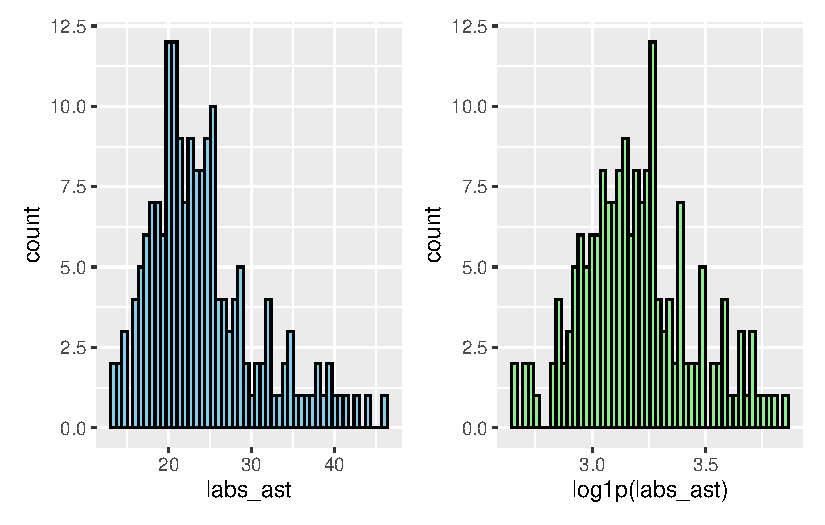
\includegraphics{Outcomes_V1V2V3_files/figure-pdf/labs_ast_1-1.pdf}

\begin{Shaded}
\begin{Highlighting}[]
\CommentTok{\# LMM}
\NormalTok{labs\_ast\_model }\OtherTok{\textless{}{-}} \FunctionTok{lmer}\NormalTok{(}\FunctionTok{log1p}\NormalTok{(labs\_ast) }\SpecialCharTok{\textasciitilde{}}\NormalTok{ allocation\_group }\SpecialCharTok{*}\NormalTok{ visit }\SpecialCharTok{+}\NormalTok{ (}\DecValTok{1} \SpecialCharTok{|}\NormalTok{ record\_id), }\AttributeTok{data =}\NormalTok{ data\_model)}
\FunctionTok{check\_collinearity}\NormalTok{(labs\_ast\_model)}
\end{Highlighting}
\end{Shaded}

\begin{verbatim}
# Check for Multicollinearity

Low Correlation

                   Term  VIF   VIF 95% CI Increased SE Tolerance
       allocation_group 1.39 [1.21, 1.74]         1.18      0.72
                  visit 3.53 [2.81, 4.54]         1.88      0.28
 allocation_group:visit 4.18 [3.30, 5.39]         2.04      0.24
 Tolerance 95% CI
     [0.57, 0.83]
     [0.22, 0.36]
     [0.19, 0.30]
\end{verbatim}

\begin{Shaded}
\begin{Highlighting}[]
\CommentTok{\# Sensitivity analysis}
\NormalTok{labs\_ast\_model\_check }\OtherTok{\textless{}{-}} \FunctionTok{sensitivity\_check\_lmer}\NormalTok{(}
    \AttributeTok{model =}\NormalTok{ labs\_ast\_model,}
    \AttributeTok{id\_var =} \StringTok{"record\_id"}\NormalTok{,}
    \AttributeTok{top\_n =} \DecValTok{5}\NormalTok{)}

\CommentTok{\# LMM Sensitivity}
\NormalTok{labs\_ast\_model\_sens }\OtherTok{\textless{}{-}} \FunctionTok{update}\NormalTok{(}\AttributeTok{object =}\NormalTok{ labs\_ast\_model,}
                              \AttributeTok{subset =} \SpecialCharTok{!}\NormalTok{(record\_id }\SpecialCharTok{\%in\%}\NormalTok{ labs\_ast\_model\_check}\SpecialCharTok{$}\NormalTok{influential\_ids))}
\CommentTok{\# Influential IDS}
\NormalTok{labs\_ast\_model\_check}\SpecialCharTok{$}\NormalTok{influential\_ids}
\end{Highlighting}
\end{Shaded}

\begin{verbatim}
[1] "4"  "14" "33" "61" "16"
\end{verbatim}

\paragraph{Resumo dos modelos}\label{resumo-dos-modelos}

\begin{Shaded}
\begin{Highlighting}[]
\CommentTok{\# Model comparison}
\FunctionTok{summary}\NormalTok{(labs\_ast\_model)}
\end{Highlighting}
\end{Shaded}

\begin{verbatim}
Linear mixed model fit by REML. t-tests use Satterthwaite's method [
lmerModLmerTest]
Formula: log1p(labs_ast) ~ allocation_group * visit + (1 | record_id)
   Data: data_model

REML criterion at convergence: 5.8

Scaled residuals: 
     Min       1Q   Median       3Q      Max 
-2.72864 -0.55023 -0.04259  0.56429  2.70480 

Random effects:
 Groups    Name        Variance Std.Dev.
 record_id (Intercept) 0.03007  0.1734  
 Residual              0.03385  0.1840  
Number of obs: 179, groups:  record_id, 75

Fixed effects:
                                 Estimate Std. Error         df t value
(Intercept)                      3.211717   0.041563 126.794430  77.273
allocation_groupGrupo B         -0.020671   0.058392 126.794430  -0.354
visit2                          -0.008428   0.045718 106.361849  -0.184
visit3                          -0.009289   0.049356 109.412475  -0.188
allocation_groupGrupo B:visit2  -0.015833   0.066802 109.278386  -0.237
allocation_groupGrupo B:visit3   0.025422   0.071565 111.735957   0.355
                               Pr(>|t|)    
(Intercept)                      <2e-16 ***
allocation_groupGrupo B           0.724    
visit2                            0.854    
visit3                            0.851    
allocation_groupGrupo B:visit2    0.813    
allocation_groupGrupo B:visit3    0.723    
---
Signif. codes:  0 '***' 0.001 '**' 0.01 '*' 0.05 '.' 0.1 ' ' 1

Correlation of Fixed Effects:
            (Intr) all_GB visit2 visit3 a_GB:2
allctn_grGB -0.712                            
visit2      -0.481  0.343                     
visit3      -0.446  0.317  0.442              
allctn_GB:2  0.330 -0.463 -0.684 -0.303       
allctn_GB:3  0.308 -0.432 -0.305 -0.690  0.424
\end{verbatim}

\begin{Shaded}
\begin{Highlighting}[]
\FunctionTok{summary}\NormalTok{(labs\_ast\_model\_sens)}
\end{Highlighting}
\end{Shaded}

\begin{verbatim}
Linear mixed model fit by REML. t-tests use Satterthwaite's method [
lmerModLmerTest]
Formula: log1p(labs_ast) ~ allocation_group * visit + (1 | record_id)
   Data: data_model
 Subset: !(record_id %in% labs_ast_model_check$influential_ids)

REML criterion at convergence: -33.2

Scaled residuals: 
     Min       1Q   Median       3Q      Max 
-1.91122 -0.53274 -0.03816  0.58631  1.89195 

Random effects:
 Groups    Name        Variance Std.Dev.
 record_id (Intercept) 0.03382  0.1839  
 Residual              0.02259  0.1503  
Number of obs: 166, groups:  record_id, 70

Fixed effects:
                                Estimate Std. Error        df t value Pr(>|t|)
(Intercept)                      3.22105    0.04015 100.92953  80.229   <2e-16
allocation_groupGrupo B         -0.04417    0.05678 100.92953  -0.778    0.438
visit2                          -0.01756    0.03879  95.56884  -0.453    0.652
visit3                          -0.03571    0.04157  97.13735  -0.859    0.392
allocation_groupGrupo B:visit2  -0.02157    0.05710  97.80899  -0.378    0.706
allocation_groupGrupo B:visit3   0.06882    0.06184  99.31712   1.113    0.268
                                  
(Intercept)                    ***
allocation_groupGrupo B           
visit2                            
visit3                            
allocation_groupGrupo B:visit2    
allocation_groupGrupo B:visit3    
---
Signif. codes:  0 '***' 0.001 '**' 0.01 '*' 0.05 '.' 0.1 ' ' 1

Correlation of Fixed Effects:
            (Intr) all_GB visit2 visit3 a_GB:2
allctn_grGB -0.707                            
visit2      -0.414  0.293                     
visit3      -0.387  0.274  0.450              
allctn_GB:2  0.282 -0.398 -0.679 -0.306       
allctn_GB:3  0.260 -0.368 -0.302 -0.672  0.430
\end{verbatim}

\begin{Shaded}
\begin{Highlighting}[]
\NormalTok{labs\_ast\_model\_check}\SpecialCharTok{$}\NormalTok{comparison\_table}
\end{Highlighting}
\end{Shaded}

\begin{verbatim}
# A tibble: 16 x 6
   Model       term                      estimate std.error statistic    p.value
   <chr>       <chr>                        <dbl>     <dbl>     <dbl>      <dbl>
 1 Original    (Intercept)                3.21       0.0416    77.3    1.64e-108
 2 Sensitivity (Intercept)                3.22       0.0401    80.2    3.09e- 93
 3 Original    allocation_groupGrupo B   -0.0207     0.0584    -0.354  7.24e-  1
 4 Sensitivity allocation_groupGrupo B   -0.0442     0.0568    -0.778  4.38e-  1
 5 Original    allocation_groupGrupo B:~ -0.0158     0.0668    -0.237  8.13e-  1
 6 Sensitivity allocation_groupGrupo B:~ -0.0216     0.0571    -0.378  7.06e-  1
 7 Original    allocation_groupGrupo B:~  0.0254     0.0716     0.355  7.23e-  1
 8 Sensitivity allocation_groupGrupo B:~  0.0688     0.0618     1.11   2.68e-  1
 9 Original    sd__(Intercept)            0.173     NA         NA     NA        
10 Sensitivity sd__(Intercept)            0.184     NA         NA     NA        
11 Original    sd__Observation            0.184     NA         NA     NA        
12 Sensitivity sd__Observation            0.150     NA         NA     NA        
13 Original    visit2                    -0.00843    0.0457    -0.184  8.54e-  1
14 Sensitivity visit2                    -0.0176     0.0388    -0.453  6.52e-  1
15 Original    visit3                    -0.00929    0.0494    -0.188  8.51e-  1
16 Sensitivity visit3                    -0.0357     0.0416    -0.859  3.92e-  1
\end{verbatim}

\begin{Shaded}
\begin{Highlighting}[]
\NormalTok{performance}\SpecialCharTok{::}\FunctionTok{compare\_performance}\NormalTok{(labs\_ast\_model, labs\_ast\_model\_sens)}
\end{Highlighting}
\end{Shaded}

\begin{verbatim}
When comparing models, please note that probably not all models were fit
  from same data.
\end{verbatim}

\begin{verbatim}
# Comparison of Model Performance Indices

Name                |           Model |  AIC (weights) | AICc (weights)
-----------------------------------------------------------------------
labs_ast_model      | lmerModLmerTest | 1139.5 (<.001) | 1140.3 (<.001)
labs_ast_model_sens | lmerModLmerTest | 1014.1 (>.999) | 1015.0 (>.999)

Name                |  BIC (weights) | R2 (cond.) | R2 (marg.) |   ICC |  RMSE | Sigma
--------------------------------------------------------------------------------------
labs_ast_model      | 1165.0 (<.001) |      0.472 |      0.003 | 0.470 | 0.154 | 0.184
labs_ast_model_sens | 1039.0 (>.999) |      0.605 |      0.013 | 0.600 | 0.122 | 0.150
\end{verbatim}

\begin{Shaded}
\begin{Highlighting}[]
\NormalTok{performance}\SpecialCharTok{::}\FunctionTok{check\_model}\NormalTok{(labs\_ast\_model)}
\end{Highlighting}
\end{Shaded}

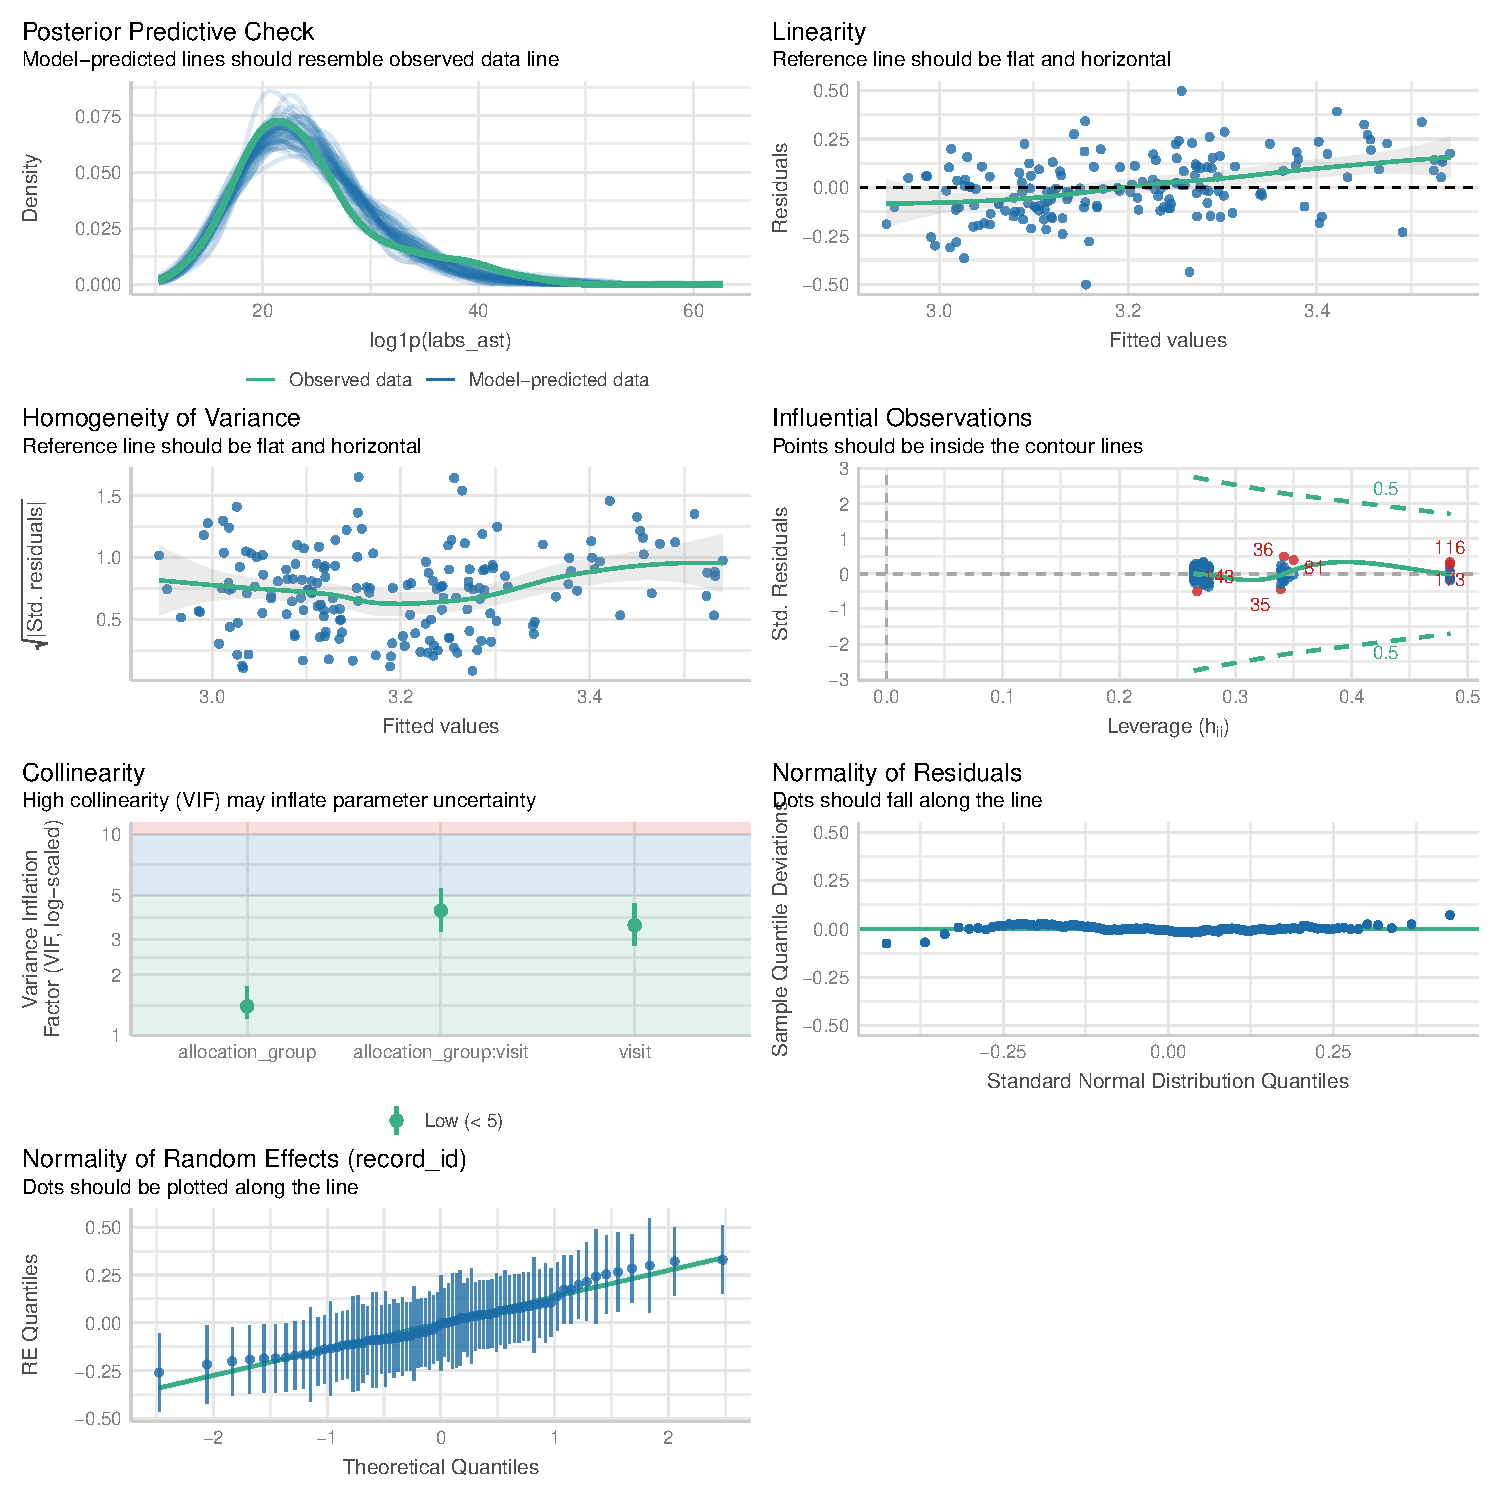
\includegraphics{Outcomes_V1V2V3_files/figure-pdf/labs_ast_4-1.pdf}

\begin{Shaded}
\begin{Highlighting}[]
\NormalTok{performance}\SpecialCharTok{::}\FunctionTok{check\_model}\NormalTok{(labs\_ast\_model\_sens)}
\end{Highlighting}
\end{Shaded}

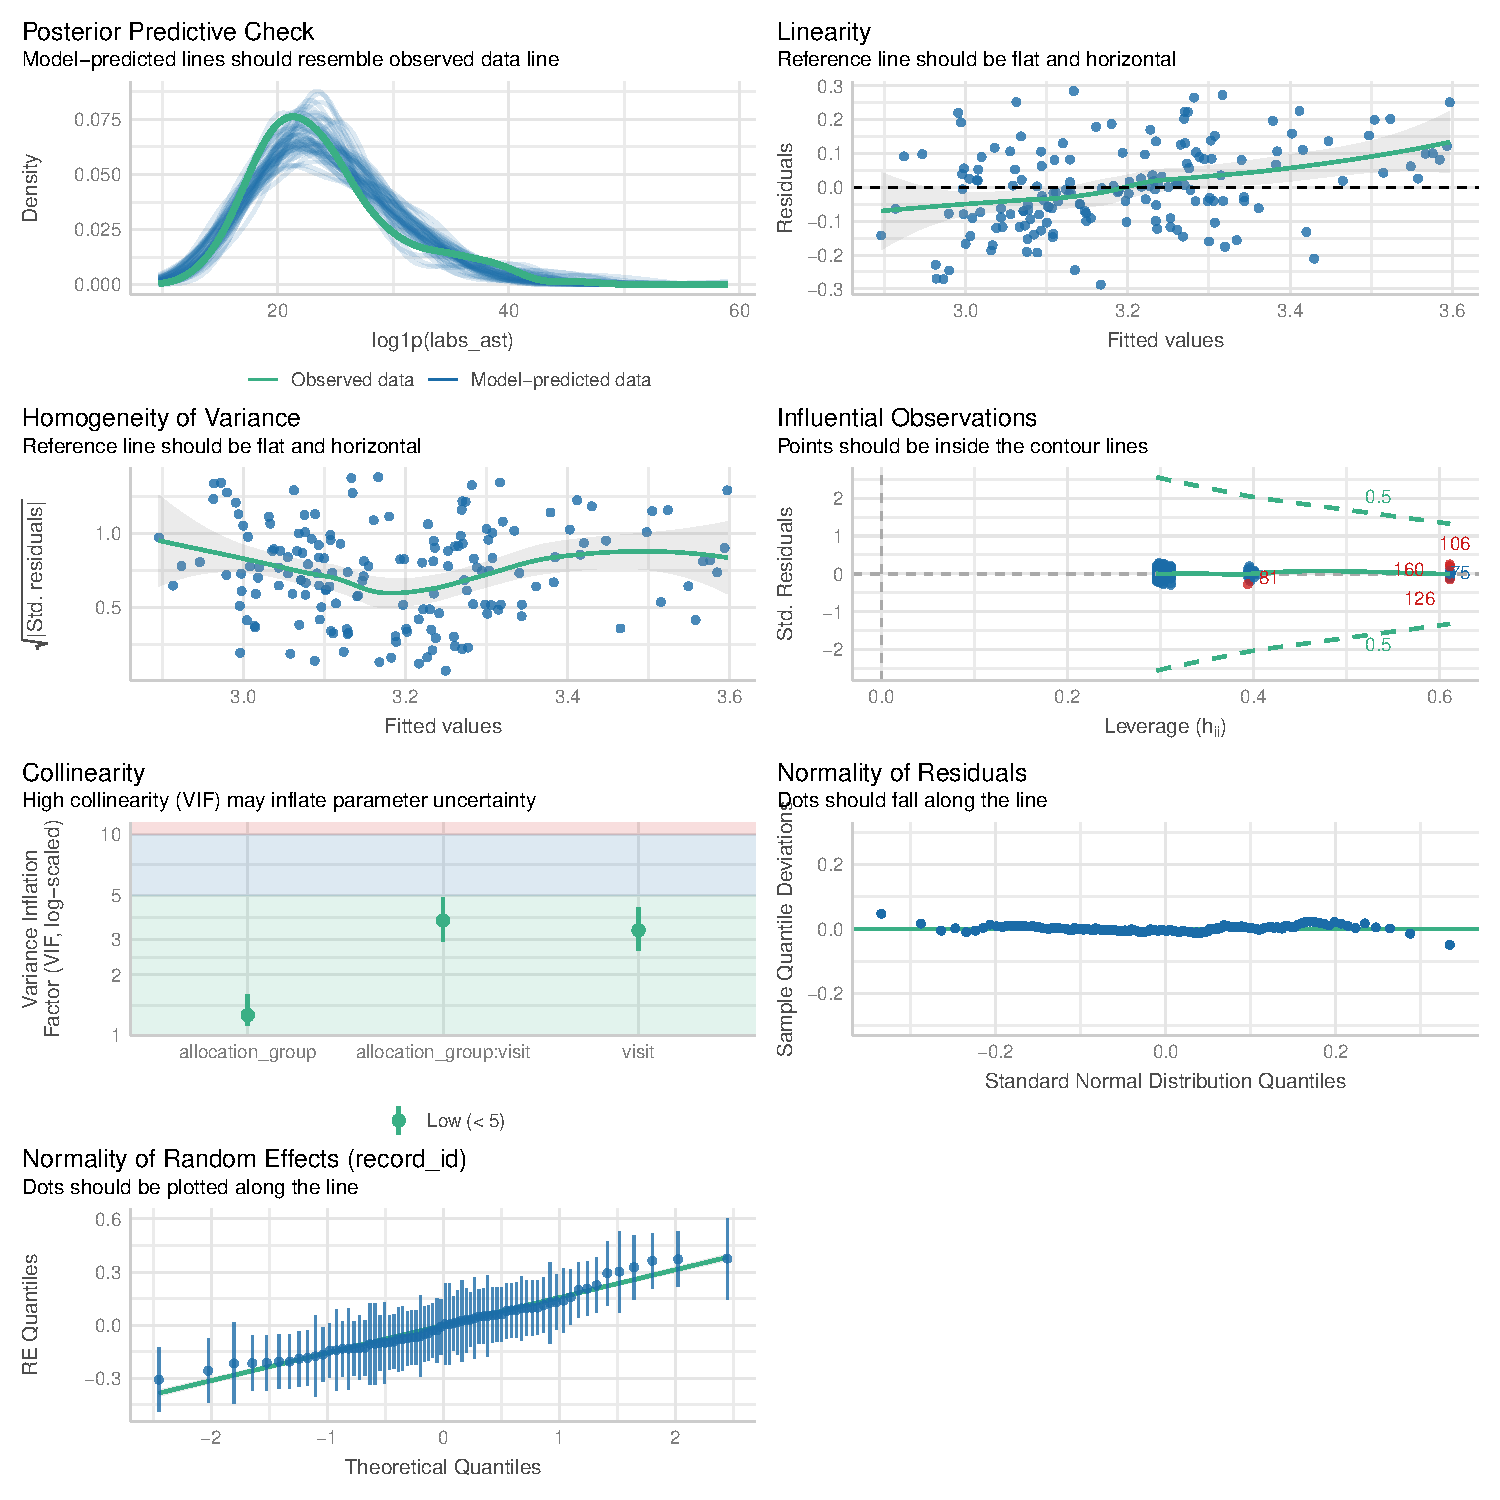
\includegraphics{Outcomes_V1V2V3_files/figure-pdf/labs_ast_4-2.pdf}

\paragraph{Médias Marginais
Estimadas}\label{muxe9dias-marginais-estimadas}

\begin{Shaded}
\begin{Highlighting}[]
\CommentTok{\# Get EMMs for each group at each visit}
\NormalTok{labs\_ast\_raw\_emm }\OtherTok{\textless{}{-}}\NormalTok{ emmeans}\SpecialCharTok{::}\FunctionTok{emmeans}\NormalTok{(}
\NormalTok{    labs\_ast\_model, }
    \SpecialCharTok{\textasciitilde{}}\NormalTok{ allocation\_group }\SpecialCharTok{*}\NormalTok{ visit}
\NormalTok{)}

\NormalTok{labs\_ast\_raw\_emm }\OtherTok{\textless{}{-}} \FunctionTok{regrid}\NormalTok{(labs\_ast\_raw\_emm)}

\CommentTok{\# Table of marginal means}
\NormalTok{labs\_ast\_raw\_emm}
\end{Highlighting}
\end{Shaded}

\begin{verbatim}
 allocation_group visit response    SE  df lower.CL upper.CL
 Grupo A          1         23.8 1.030 128     21.8     25.9
 Grupo B          1         23.3 0.997 128     21.3     25.3
 Grupo A          2         23.6 1.100 142     21.4     25.8
 Grupo B          2         22.7 1.130 155     20.5     25.0
 Grupo A          3         23.6 1.190 157     21.2     25.9
 Grupo B          3         23.7 1.260 164     21.2     26.2

Degrees-of-freedom method: inherited from kenward-roger when re-gridding 
Confidence level used: 0.95 
\end{verbatim}

\begin{Shaded}
\begin{Highlighting}[]
\CommentTok{\# Pairwise comparisons: Between groups at each visit}
\NormalTok{emmeans}\SpecialCharTok{::}\FunctionTok{contrast}\NormalTok{(labs\_ast\_raw\_emm, }\AttributeTok{method =} \StringTok{"pairwise"}\NormalTok{, }\AttributeTok{by =} \StringTok{"visit"}\NormalTok{, }\AttributeTok{adjust =} \StringTok{"bonferroni"}\NormalTok{) }\SpecialCharTok{\%\textgreater{}\%} \FunctionTok{summary}\NormalTok{(}\AttributeTok{infer =} \FunctionTok{c}\NormalTok{(}\ConstantTok{TRUE}\NormalTok{, }\ConstantTok{TRUE}\NormalTok{))}
\end{Highlighting}
\end{Shaded}

\begin{verbatim}
visit = 1:
 contrast          estimate   SE  df lower.CL upper.CL t.ratio p.value
 Grupo A - Grupo B    0.508 1.43 128    -2.33     3.35   0.354  0.7240

visit = 2:
 contrast          estimate   SE  df lower.CL upper.CL t.ratio p.value
 Grupo A - Grupo B    0.882 1.58 142    -2.24     4.00   0.559  0.5771

visit = 3:
 contrast          estimate   SE  df lower.CL upper.CL t.ratio p.value
 Grupo A - Grupo B   -0.117 1.73 157    -3.54     3.31  -0.068  0.9462

Degrees-of-freedom method: inherited from kenward-roger when re-gridding 
Confidence level used: 0.95 
\end{verbatim}

\begin{Shaded}
\begin{Highlighting}[]
\CommentTok{\# Pairwise comparisons: Changes over time within each group}
\NormalTok{emmeans}\SpecialCharTok{::}\FunctionTok{contrast}\NormalTok{(labs\_ast\_raw\_emm, }\AttributeTok{method =} \StringTok{"pairwise"}\NormalTok{, }\AttributeTok{by =} \StringTok{"allocation\_group"}\NormalTok{, }\AttributeTok{adjust =} \StringTok{"bonferroni"}\NormalTok{) }\SpecialCharTok{\%\textgreater{}\%} \FunctionTok{summary}\NormalTok{(}\AttributeTok{infer =} \FunctionTok{c}\NormalTok{(}\ConstantTok{TRUE}\NormalTok{, }\ConstantTok{TRUE}\NormalTok{))}
\end{Highlighting}
\end{Shaded}

\begin{verbatim}
allocation_group = Grupo A:
 contrast        estimate   SE  df lower.CL upper.CL t.ratio p.value
 visit1 - visit2   0.2083 1.13 128    -2.53     2.95   0.184  1.0000
 visit1 - visit3   0.2295 1.22 128    -2.73     3.19   0.188  1.0000
 visit2 - visit3   0.0212 1.24 142    -2.98     3.02   0.017  1.0000

allocation_group = Grupo B:
 contrast        estimate   SE  df lower.CL upper.CL t.ratio p.value
 visit1 - visit2   0.5828 1.17 128    -2.25     3.42   0.499  1.0000
 visit1 - visit3  -0.3954 1.28 128    -3.49     2.70  -0.310  1.0000
 visit2 - visit3  -0.9782 1.33 155    -4.20     2.24  -0.735  1.0000

Degrees-of-freedom method: inherited from kenward-roger when re-gridding 
Confidence level used: 0.95 
Conf-level adjustment: bonferroni method for 3 estimates 
P value adjustment: bonferroni method for 3 tests 
\end{verbatim}

\begin{Shaded}
\begin{Highlighting}[]
\CommentTok{\# Plot of marginal means}
\FunctionTok{plot}\NormalTok{(labs\_ast\_raw\_emm, }\AttributeTok{comparisons =} \ConstantTok{TRUE}\NormalTok{)}
\end{Highlighting}
\end{Shaded}

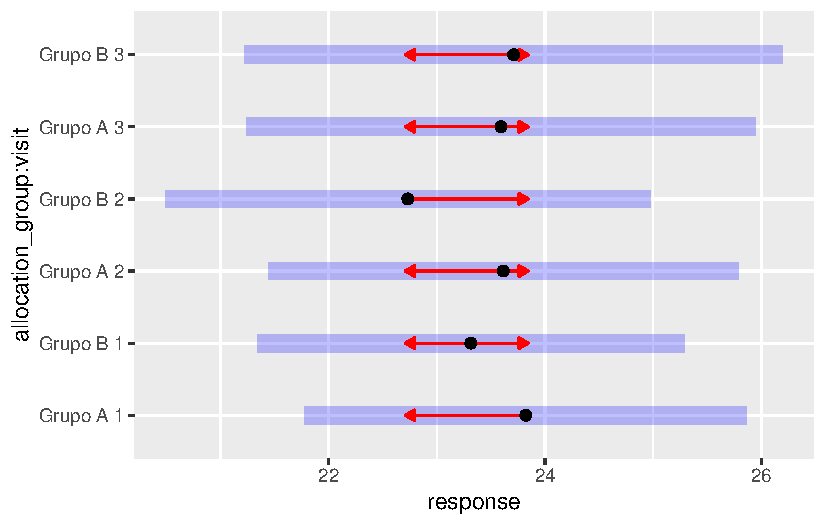
\includegraphics{Outcomes_V1V2V3_files/figure-pdf/labs_ast_raw_emm-1.pdf}

\begin{Shaded}
\begin{Highlighting}[]
\CommentTok{\# Get EMMs for each group at each visit}
\NormalTok{labs\_ast\_emm }\OtherTok{\textless{}{-}}\NormalTok{ emmeans}\SpecialCharTok{::}\FunctionTok{emmeans}\NormalTok{(}
\NormalTok{    labs\_ast\_model\_sens, }
    \SpecialCharTok{\textasciitilde{}}\NormalTok{ allocation\_group }\SpecialCharTok{*}\NormalTok{ visit}
\NormalTok{)}

\NormalTok{labs\_ast\_emm }\OtherTok{\textless{}{-}} \FunctionTok{regrid}\NormalTok{(labs\_ast\_emm)}

\CommentTok{\# Table of marginal means}
\NormalTok{labs\_ast\_emm}
\end{Highlighting}
\end{Shaded}

\begin{verbatim}
 allocation_group visit response    SE  df lower.CL upper.CL
 Grupo A          1         24.1 1.010 104     22.1     26.0
 Grupo B          1         23.0 0.962 104     21.1     24.9
 Grupo A          2         23.6 1.050 118     21.5     25.7
 Grupo B          2         22.1 1.050 131     20.0     24.1
 Grupo A          3         23.2 1.100 132     21.0     25.3
 Grupo B          3         23.8 1.220 146     21.4     26.2

Degrees-of-freedom method: inherited from kenward-roger when re-gridding 
Confidence level used: 0.95 
\end{verbatim}

\begin{Shaded}
\begin{Highlighting}[]
\CommentTok{\# Pairwise comparisons: Between groups at each visit}
\NormalTok{emmeans}\SpecialCharTok{::}\FunctionTok{contrast}\NormalTok{(labs\_ast\_emm, }\AttributeTok{method =} \StringTok{"pairwise"}\NormalTok{, }\AttributeTok{by =} \StringTok{"visit"}\NormalTok{, }\AttributeTok{adjust =} \StringTok{"bonferroni"}\NormalTok{) }\SpecialCharTok{\%\textgreater{}\%} \FunctionTok{summary}\NormalTok{(}\AttributeTok{infer =} \FunctionTok{c}\NormalTok{(}\ConstantTok{TRUE}\NormalTok{, }\ConstantTok{TRUE}\NormalTok{))}
\end{Highlighting}
\end{Shaded}

\begin{verbatim}
visit = 1:
 contrast          estimate   SE  df lower.CL upper.CL t.ratio p.value
 Grupo A - Grupo B    1.083 1.39 104    -1.68     3.84   0.778  0.4386

visit = 2:
 contrast          estimate   SE  df lower.CL upper.CL t.ratio p.value
 Grupo A - Grupo B    1.566 1.49 118    -1.38     4.51   1.052  0.2948

visit = 3:
 contrast          estimate   SE  df lower.CL upper.CL t.ratio p.value
 Grupo A - Grupo B   -0.603 1.64 132    -3.85     2.64  -0.368  0.7136

Degrees-of-freedom method: inherited from kenward-roger when re-gridding 
Confidence level used: 0.95 
\end{verbatim}

\begin{Shaded}
\begin{Highlighting}[]
\CommentTok{\# Pairwise comparisons: Changes over time within each group}
\NormalTok{emmeans}\SpecialCharTok{::}\FunctionTok{contrast}\NormalTok{(labs\_ast\_emm, }\AttributeTok{method =} \StringTok{"pairwise"}\NormalTok{, }\AttributeTok{by =} \StringTok{"allocation\_group"}\NormalTok{, }\AttributeTok{adjust =} \StringTok{"bonferroni"}\NormalTok{) }\SpecialCharTok{\%\textgreater{}\%} \FunctionTok{summary}\NormalTok{(}\AttributeTok{infer =} \FunctionTok{c}\NormalTok{(}\ConstantTok{TRUE}\NormalTok{, }\ConstantTok{TRUE}\NormalTok{))}
\end{Highlighting}
\end{Shaded}

\begin{verbatim}
allocation_group = Grupo A:
 contrast        estimate    SE  df lower.CL upper.CL t.ratio p.value
 visit1 - visit2    0.436 0.963 104    -1.91     2.78   0.453  1.0000
 visit1 - visit3    0.879 1.020 104    -1.60     3.36   0.861  1.0000
 visit2 - visit3    0.443 1.030 118    -2.06     2.94   0.430  1.0000

allocation_group = Grupo B:
 contrast        estimate    SE  df lower.CL upper.CL t.ratio p.value
 visit1 - visit2    0.920 0.983 104    -1.47     3.31   0.936  1.0000
 visit1 - visit3   -0.807 1.130 104    -3.55     1.93  -0.716  1.0000
 visit2 - visit3   -1.727 1.150 131    -4.51     1.06  -1.505  0.4043

Degrees-of-freedom method: inherited from kenward-roger when re-gridding 
Confidence level used: 0.95 
Conf-level adjustment: bonferroni method for 3 estimates 
P value adjustment: bonferroni method for 3 tests 
\end{verbatim}

\begin{Shaded}
\begin{Highlighting}[]
\CommentTok{\# Plot of marginal means}
\FunctionTok{plot}\NormalTok{(labs\_ast\_emm, }\AttributeTok{comparisons =} \ConstantTok{TRUE}\NormalTok{)}
\end{Highlighting}
\end{Shaded}

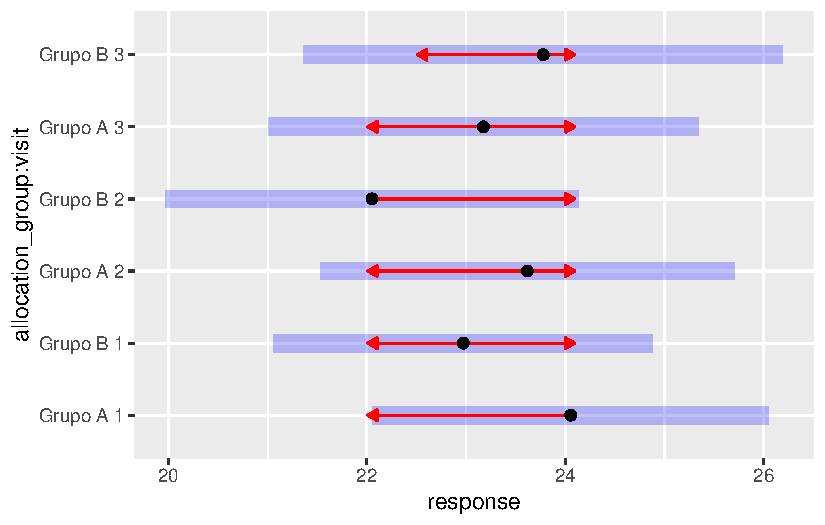
\includegraphics{Outcomes_V1V2V3_files/figure-pdf/labs_ast_sens_emm-1.pdf}

\begin{Shaded}
\begin{Highlighting}[]
\FunctionTok{ggplot}\NormalTok{(}
    \AttributeTok{data =}\NormalTok{ data\_model, }
    \FunctionTok{aes}\NormalTok{(}
        \AttributeTok{x =} \FunctionTok{as.factor}\NormalTok{(visit),}
        \AttributeTok{y =}\NormalTok{ labs\_ast,}
        \AttributeTok{group =}\NormalTok{ record\_id,}
\NormalTok{    )}
\NormalTok{) }\SpecialCharTok{+}
    \FunctionTok{geom\_line}\NormalTok{(}\AttributeTok{alpha =} \FloatTok{0.5}\NormalTok{) }\SpecialCharTok{+}
    \FunctionTok{geom\_point}\NormalTok{(}\AttributeTok{alpha =} \FloatTok{0.7}\NormalTok{) }\SpecialCharTok{+}
    \FunctionTok{geom\_smooth}\NormalTok{(}
        \FunctionTok{aes}\NormalTok{(}\AttributeTok{group =}\NormalTok{ allocation\_group),}
        \AttributeTok{method =} \StringTok{"lm"}\NormalTok{,}
        \AttributeTok{se =} \ConstantTok{TRUE}\NormalTok{,}
        \AttributeTok{linewidth =} \DecValTok{1}
\NormalTok{    ) }\SpecialCharTok{+}
    \FunctionTok{labs}\NormalTok{(}\AttributeTok{title =} \StringTok{"All data"}\NormalTok{) }\SpecialCharTok{+}
    \FunctionTok{facet\_wrap}\NormalTok{(}\SpecialCharTok{\textasciitilde{}}\NormalTok{ allocation\_group)}
\end{Highlighting}
\end{Shaded}

\begin{verbatim}
`geom_smooth()` using formula = 'y ~ x'
\end{verbatim}

\begin{verbatim}
Warning: Removed 10 rows containing non-finite outside the scale range
(`stat_smooth()`).
\end{verbatim}

\begin{verbatim}
Warning: Removed 8 rows containing missing values or values outside the scale range
(`geom_line()`).
\end{verbatim}

\begin{verbatim}
Warning: Removed 10 rows containing missing values or values outside the scale range
(`geom_point()`).
\end{verbatim}

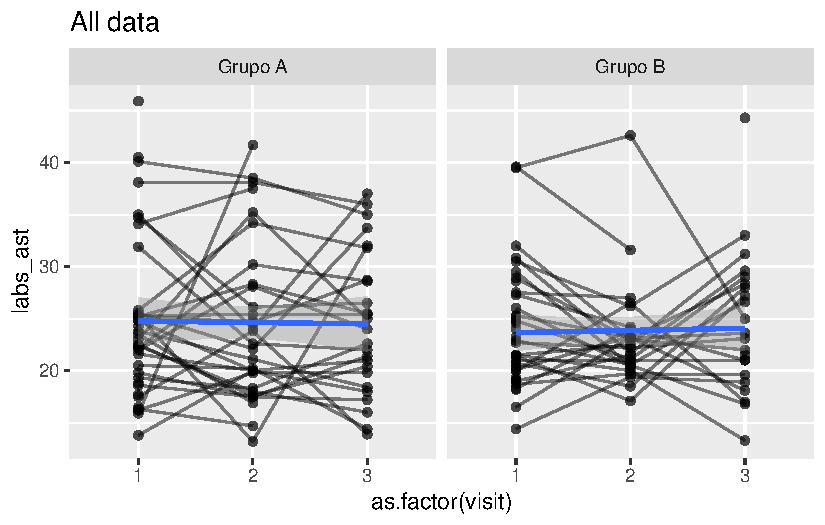
\includegraphics{Outcomes_V1V2V3_files/figure-pdf/labs_ast_6-1.pdf}

\begin{Shaded}
\begin{Highlighting}[]
\NormalTok{data\_model }\SpecialCharTok{\%\textgreater{}\%} 
    \FunctionTok{filter}\NormalTok{(}
        \SpecialCharTok{!}\NormalTok{(record\_id }\SpecialCharTok{\%in\%}\NormalTok{ labs\_ast\_model\_check}\SpecialCharTok{$}\NormalTok{influential\_ids)}
\NormalTok{    ) }\SpecialCharTok{\%\textgreater{}\%} 
    \FunctionTok{ggplot}\NormalTok{(}
        \FunctionTok{aes}\NormalTok{(}
            \AttributeTok{x =} \FunctionTok{as.factor}\NormalTok{(visit),}
            \AttributeTok{y =}\NormalTok{ labs\_ast,}
            \AttributeTok{group =}\NormalTok{ record\_id,}
\NormalTok{        )}
\NormalTok{    ) }\SpecialCharTok{+}
    \FunctionTok{geom\_line}\NormalTok{(}\AttributeTok{alpha =} \FloatTok{0.5}\NormalTok{) }\SpecialCharTok{+}
    \FunctionTok{geom\_point}\NormalTok{(}\AttributeTok{alpha =} \FloatTok{0.7}\NormalTok{) }\SpecialCharTok{+}
    \FunctionTok{geom\_smooth}\NormalTok{(}
        \FunctionTok{aes}\NormalTok{(}\AttributeTok{group =}\NormalTok{ allocation\_group),}
        \AttributeTok{method =} \StringTok{"lm"}\NormalTok{,}
        \AttributeTok{se =} \ConstantTok{TRUE}\NormalTok{,}
        \AttributeTok{linewidth =} \DecValTok{1}
\NormalTok{    ) }\SpecialCharTok{+}
    \FunctionTok{labs}\NormalTok{(}\AttributeTok{title =} \StringTok{"Sensitivity analysis"}\NormalTok{) }\SpecialCharTok{+}
    \FunctionTok{facet\_wrap}\NormalTok{(}\SpecialCharTok{\textasciitilde{}}\NormalTok{ allocation\_group)}
\end{Highlighting}
\end{Shaded}

\begin{verbatim}
`geom_smooth()` using formula = 'y ~ x'
\end{verbatim}

\begin{verbatim}
Warning: Removed 9 rows containing non-finite outside the scale range
(`stat_smooth()`).
\end{verbatim}

\begin{verbatim}
Warning: Removed 8 rows containing missing values or values outside the scale range
(`geom_line()`).
\end{verbatim}

\begin{verbatim}
Warning: Removed 9 rows containing missing values or values outside the scale range
(`geom_point()`).
\end{verbatim}

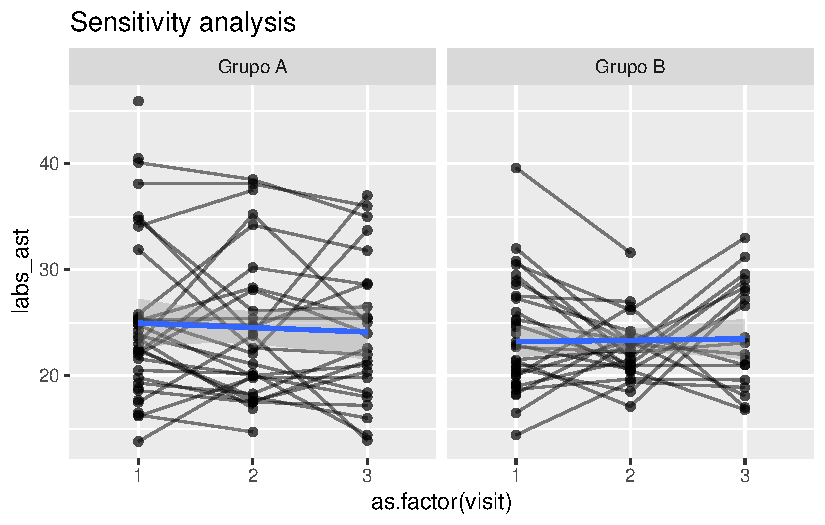
\includegraphics{Outcomes_V1V2V3_files/figure-pdf/labs_ast_6-2.pdf}

\paragraph{Resultado}\label{resultado}

No modelo ajustado para os níveis de AST, não foram observadas
diferenças estatisticamente significativas entre os grupos em nenhum dos
três momentos avaliados. Da mesma forma, não houve mudanças
significativas ao longo do tempo dentro de cada grupo. As estimativas,
intervalos de confiança de 95\% e valores de p estão apresentados na
Tabela @tbl:ast.

\begin{longtable}[]{@{}
  >{\raggedright\arraybackslash}p{(\columnwidth - 8\tabcolsep) * \real{0.2500}}
  >{\raggedright\arraybackslash}p{(\columnwidth - 8\tabcolsep) * \real{0.2826}}
  >{\raggedright\arraybackslash}p{(\columnwidth - 8\tabcolsep) * \real{0.1304}}
  >{\raggedright\arraybackslash}p{(\columnwidth - 8\tabcolsep) * \real{0.2391}}
  >{\raggedright\arraybackslash}p{(\columnwidth - 8\tabcolsep) * \real{0.0978}}@{}}
\caption{Diferenças estimadas dos níveis de Aspartato Aminotransferase
(AST) entre os grupos de alocação (placebo vs Eclipta) e entre visitas
dentro de cada grupo \{\#tbl:ast\}}\tabularnewline
\toprule\noalign{}
\begin{minipage}[b]{\linewidth}\raggedright
Grupo de comparação
\end{minipage} & \begin{minipage}[b]{\linewidth}\raggedright
Comparação
\end{minipage} & \begin{minipage}[b]{\linewidth}\raggedright
Estimativa
\end{minipage} & \begin{minipage}[b]{\linewidth}\raggedright
IC 95\%
\end{minipage} & \begin{minipage}[b]{\linewidth}\raggedright
p-valor
\end{minipage} \\
\midrule\noalign{}
\endfirsthead
\toprule\noalign{}
\begin{minipage}[b]{\linewidth}\raggedright
Grupo de comparação
\end{minipage} & \begin{minipage}[b]{\linewidth}\raggedright
Comparação
\end{minipage} & \begin{minipage}[b]{\linewidth}\raggedright
Estimativa
\end{minipage} & \begin{minipage}[b]{\linewidth}\raggedright
IC 95\%
\end{minipage} & \begin{minipage}[b]{\linewidth}\raggedright
p-valor
\end{minipage} \\
\midrule\noalign{}
\endhead
\bottomrule\noalign{}
\endlastfoot
Entre grupos & Visita 1 & 0,51 & {[}-2,33 ; 3,35{]} & 0,724 \\
Entre grupos & Visita 2 & 0,88 & {[}-2,24 ; 4,00{]} & 0,577 \\
Entre grupos & Visita 3 & -0,12 & {[}-3,54 ; 3,31{]} & 0,946 \\
Grupo Placebo & Visita 1 - Visita 2 & 0,21 & {[}-2,53 ; 2,95{]} &
1,000 \\
Grupo Placebo & Visita 1 - Visita 3 & 0,23 & {[}-2,73 ; 3,19{]} &
1,000 \\
Grupo Placebo & Visita 2 - Visita 3 & 0,02 & {[}-2,98 ; 3,02{]} &
1,000 \\
Grupo Eclipta & Visita 1 - Visita 2 & 0,58 & {[}-2,25 ; 3,42{]} &
1,000 \\
Grupo Eclipta & Visita 1 - Visita 3 & -0,40 & {[}-3,49 ; 2,70{]} &
1,000 \\
Grupo Eclipta & Visita 2 - Visita 3 & -0,98 & {[}-4,20 ; 2,24{]} &
1,000 \\
\end{longtable}

As médias marginais estimadas (EMMs) dos níveis de AST permaneceram
estáveis ao longo do tempo e semelhantes entre os grupos. Esses achados
sugerem que não houve efeito diferencial entre as intervenções, nem
alterações clínicas relevantes nos níveis de AST durante o período de
acompanhamento.

\subsubsection{Alanina Aminotransferase}\label{alanina-aminotransferase}

\begin{Shaded}
\begin{Highlighting}[]
\CommentTok{\# Plot 1: Raw data}
\NormalTok{labs\_alt\_hist\_1 }\OtherTok{\textless{}{-}}\NormalTok{ data\_model }\SpecialCharTok{\%\textgreater{}\%} 
    \CommentTok{\#filter(}
    \CommentTok{\#    labs\_alt \textless{} 300}
    \CommentTok{\#) \%\textgreater{}\% }
    \FunctionTok{ggplot}\NormalTok{(}\FunctionTok{aes}\NormalTok{(}\AttributeTok{x =}\NormalTok{ labs\_alt)) }\SpecialCharTok{+} 
    \FunctionTok{geom\_histogram}\NormalTok{(}\AttributeTok{bins =} \DecValTok{50}\NormalTok{, }\AttributeTok{fill =} \StringTok{"skyblue"}\NormalTok{, }\AttributeTok{color =} \StringTok{"black"}\NormalTok{)}

\CommentTok{\# Plot 2: Log{-}transformed data}
\NormalTok{labs\_alt\_hist\_2 }\OtherTok{\textless{}{-}}\NormalTok{ data\_model }\SpecialCharTok{\%\textgreater{}\%} 
    \CommentTok{\#filter(}
    \CommentTok{\#    labs\_alt \textless{} 300}
    \CommentTok{\#) \%\textgreater{}\%}
    \FunctionTok{ggplot}\NormalTok{(}\FunctionTok{aes}\NormalTok{(}\AttributeTok{x =} \FunctionTok{log1p}\NormalTok{(labs\_alt))) }\SpecialCharTok{+} 
    \FunctionTok{geom\_histogram}\NormalTok{(}\AttributeTok{bins =} \DecValTok{50}\NormalTok{, }\AttributeTok{fill =} \StringTok{"lightgreen"}\NormalTok{, }\AttributeTok{color =} \StringTok{"black"}\NormalTok{)}

\CommentTok{\# Combine side by side}
\NormalTok{labs\_alt\_hist\_1 }\SpecialCharTok{+}\NormalTok{ labs\_alt\_hist\_2 }\CommentTok{\# library(patchwork)}
\end{Highlighting}
\end{Shaded}

\begin{verbatim}
Warning: Removed 10 rows containing non-finite outside the scale range (`stat_bin()`).
Removed 10 rows containing non-finite outside the scale range (`stat_bin()`).
\end{verbatim}

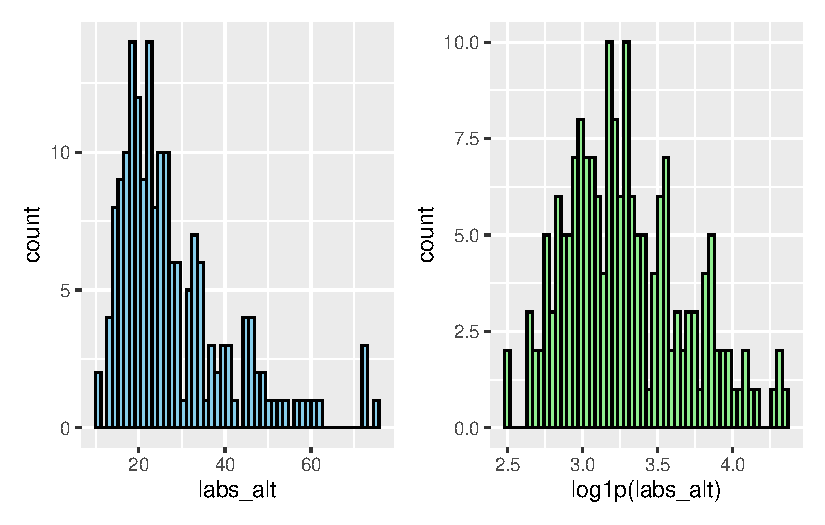
\includegraphics{Outcomes_V1V2V3_files/figure-pdf/labs_alt_1-1.pdf}

\begin{Shaded}
\begin{Highlighting}[]
\CommentTok{\# LMM}
\NormalTok{labs\_alt\_model }\OtherTok{\textless{}{-}} \FunctionTok{lmer}\NormalTok{(}\FunctionTok{log1p}\NormalTok{(labs\_alt) }\SpecialCharTok{\textasciitilde{}}\NormalTok{ allocation\_group }\SpecialCharTok{*}\NormalTok{ visit }\SpecialCharTok{+}\NormalTok{ (}\DecValTok{1} \SpecialCharTok{|}\NormalTok{ record\_id), }\AttributeTok{data =}\NormalTok{ data\_model)}
\FunctionTok{check\_collinearity}\NormalTok{(labs\_alt\_model)}
\end{Highlighting}
\end{Shaded}

\begin{verbatim}
# Check for Multicollinearity

Low Correlation

                   Term  VIF   VIF 95% CI Increased SE Tolerance
       allocation_group 1.21 [1.08, 1.54]         1.10      0.83
                  visit 3.50 [2.79, 4.49]         1.87      0.29
 allocation_group:visit 3.84 [3.04, 4.94]         1.96      0.26
 Tolerance 95% CI
     [0.65, 0.92]
     [0.22, 0.36]
     [0.20, 0.33]
\end{verbatim}

\begin{Shaded}
\begin{Highlighting}[]
\CommentTok{\# Sensitivity analysis}
\NormalTok{labs\_alt\_model\_check }\OtherTok{\textless{}{-}} \FunctionTok{sensitivity\_check\_lmer}\NormalTok{(}
    \AttributeTok{model =}\NormalTok{ labs\_alt\_model,}
    \AttributeTok{id\_var =} \StringTok{"record\_id"}\NormalTok{,}
    \AttributeTok{top\_n =} \DecValTok{5}\NormalTok{)}

\CommentTok{\# LMM Sensitivity}
\NormalTok{labs\_alt\_model\_sens }\OtherTok{\textless{}{-}} \FunctionTok{update}\NormalTok{(}\AttributeTok{object =}\NormalTok{ labs\_alt\_model,}
                              \AttributeTok{subset =} \SpecialCharTok{!}\NormalTok{(record\_id }\SpecialCharTok{\%in\%}\NormalTok{ labs\_alt\_model\_check}\SpecialCharTok{$}\NormalTok{influential\_ids))}
\CommentTok{\# Influential IDS}
\NormalTok{labs\_alt\_model\_check}\SpecialCharTok{$}\NormalTok{influential\_ids}
\end{Highlighting}
\end{Shaded}

\begin{verbatim}
[1] "33" "75" "5"  "58" "63"
\end{verbatim}

\paragraph{Resumo dos modelos}\label{resumo-dos-modelos-1}

\begin{Shaded}
\begin{Highlighting}[]
\CommentTok{\# Model comparison}
\FunctionTok{summary}\NormalTok{(labs\_alt\_model)}
\end{Highlighting}
\end{Shaded}

\begin{verbatim}
Linear mixed model fit by REML. t-tests use Satterthwaite's method [
lmerModLmerTest]
Formula: log1p(labs_alt) ~ allocation_group * visit + (1 | record_id)
   Data: data_model

REML criterion at convergence: 132.2

Scaled residuals: 
     Min       1Q   Median       3Q      Max 
-2.28166 -0.55027 -0.05275  0.54015  2.15582 

Random effects:
 Groups    Name        Variance Std.Dev.
 record_id (Intercept) 0.10863  0.3296  
 Residual              0.05485  0.2342  
Number of obs: 179, groups:  record_id, 75

Fixed effects:
                                Estimate Std. Error        df t value Pr(>|t|)
(Intercept)                      3.34045    0.06647 102.44387  50.254   <2e-16
allocation_groupGrupo B         -0.10187    0.09338 102.44387  -1.091    0.278
visit2                          -0.07956    0.05867 103.85033  -1.356    0.178
visit3                          -0.03364    0.06353 105.34376  -0.529    0.598
allocation_groupGrupo B:visit2   0.06143    0.08602 105.75034   0.714    0.477
allocation_groupGrupo B:visit3   0.07920    0.09237 106.88087   0.857    0.393
                                  
(Intercept)                    ***
allocation_groupGrupo B           
visit2                            
visit3                            
allocation_groupGrupo B:visit2    
allocation_groupGrupo B:visit3    
---
Signif. codes:  0 '***' 0.001 '**' 0.01 '*' 0.05 '.' 0.1 ' ' 1

Correlation of Fixed Effects:
            (Intr) all_GB visit2 visit3 a_GB:2
allctn_grGB -0.712                            
visit2      -0.380  0.271                     
visit3      -0.351  0.250  0.449              
allctn_GB:2  0.259 -0.364 -0.682 -0.306       
allctn_GB:3  0.241 -0.339 -0.309 -0.688  0.432
\end{verbatim}

\begin{Shaded}
\begin{Highlighting}[]
\FunctionTok{summary}\NormalTok{(labs\_alt\_model\_sens)}
\end{Highlighting}
\end{Shaded}

\begin{verbatim}
Linear mixed model fit by REML. t-tests use Satterthwaite's method [
lmerModLmerTest]
Formula: log1p(labs_alt) ~ allocation_group * visit + (1 | record_id)
   Data: data_model
 Subset: !(record_id %in% labs_alt_model_check$influential_ids)

REML criterion at convergence: 88.4

Scaled residuals: 
     Min       1Q   Median       3Q      Max 
-1.98911 -0.51655 -0.03328  0.57521  2.21076 

Random effects:
 Groups    Name        Variance Std.Dev.
 record_id (Intercept) 0.09385  0.3063  
 Residual              0.04238  0.2059  
Number of obs: 165, groups:  record_id, 70

Fixed effects:
                                Estimate Std. Error        df t value Pr(>|t|)
(Intercept)                     3.249918   0.064250 90.966334  50.582   <2e-16
allocation_groupGrupo B        -0.013075   0.088373 90.966334  -0.148    0.883
visit2                         -0.021536   0.055231 93.405160  -0.390    0.697
visit3                         -0.035422   0.060679 94.750397  -0.584    0.561
allocation_groupGrupo B:visit2 -0.009275   0.078377 94.689442  -0.118    0.906
allocation_groupGrupo B:visit3  0.043535   0.085567 95.767451   0.509    0.612
                                  
(Intercept)                    ***
allocation_groupGrupo B           
visit2                            
visit3                            
allocation_groupGrupo B:visit2    
allocation_groupGrupo B:visit3    
---
Signif. codes:  0 '***' 0.001 '**' 0.01 '*' 0.05 '.' 0.1 ' ' 1

Correlation of Fixed Effects:
            (Intr) all_GB visit2 visit3 a_GB:2
allctn_grGB -0.727                            
visit2      -0.362  0.263                     
visit3      -0.329  0.239  0.442              
allctn_GB:2  0.255 -0.351 -0.705 -0.311       
allctn_GB:3  0.234 -0.321 -0.313 -0.709  0.434
\end{verbatim}

\begin{Shaded}
\begin{Highlighting}[]
\NormalTok{labs\_alt\_model\_check}\SpecialCharTok{$}\NormalTok{comparison\_table}
\end{Highlighting}
\end{Shaded}

\begin{verbatim}
# A tibble: 16 x 6
   Model       term                       estimate std.error statistic   p.value
   <chr>       <chr>                         <dbl>     <dbl>     <dbl>     <dbl>
 1 Original    (Intercept)                 3.34       0.0665    50.3    5.32e-74
 2 Sensitivity (Intercept)                 3.25       0.0642    50.6    2.13e-68
 3 Original    allocation_groupGrupo B    -0.102      0.0934    -1.09   2.78e- 1
 4 Sensitivity allocation_groupGrupo B    -0.0131     0.0884    -0.148  8.83e- 1
 5 Original    allocation_groupGrupo B:v~  0.0614     0.0860     0.714  4.77e- 1
 6 Sensitivity allocation_groupGrupo B:v~ -0.00928    0.0784    -0.118  9.06e- 1
 7 Original    allocation_groupGrupo B:v~  0.0792     0.0924     0.857  3.93e- 1
 8 Sensitivity allocation_groupGrupo B:v~  0.0435     0.0856     0.509  6.12e- 1
 9 Original    sd__(Intercept)             0.330     NA         NA     NA       
10 Sensitivity sd__(Intercept)             0.306     NA         NA     NA       
11 Original    sd__Observation             0.234     NA         NA     NA       
12 Sensitivity sd__Observation             0.206     NA         NA     NA       
13 Original    visit2                     -0.0796     0.0587    -1.36   1.78e- 1
14 Sensitivity visit2                     -0.0215     0.0552    -0.390  6.97e- 1
15 Original    visit3                     -0.0336     0.0635    -0.529  5.98e- 1
16 Sensitivity visit3                     -0.0354     0.0607    -0.584  5.61e- 1
\end{verbatim}

\begin{Shaded}
\begin{Highlighting}[]
\NormalTok{performance}\SpecialCharTok{::}\FunctionTok{compare\_performance}\NormalTok{(labs\_alt\_model, labs\_alt\_model\_sens)}
\end{Highlighting}
\end{Shaded}

\begin{verbatim}
When comparing models, please note that probably not all models were fit
  from same data.
\end{verbatim}

\begin{verbatim}
# Comparison of Model Performance Indices

Name                |           Model |  AIC (weights) | AICc (weights)
-----------------------------------------------------------------------
labs_alt_model      | lmerModLmerTest | 1302.9 (<.001) | 1303.8 (<.001)
labs_alt_model_sens | lmerModLmerTest | 1150.5 (>.999) | 1151.4 (>.999)

Name                |  BIC (weights) | R2 (cond.) | R2 (marg.) |   ICC |  RMSE | Sigma
--------------------------------------------------------------------------------------
labs_alt_model      | 1328.4 (<.001) |      0.668 |      0.011 | 0.664 | 0.187 | 0.234
labs_alt_model_sens | 1175.3 (>.999) |      0.689 |      0.002 | 0.689 | 0.163 | 0.206
\end{verbatim}

\begin{Shaded}
\begin{Highlighting}[]
\NormalTok{performance}\SpecialCharTok{::}\FunctionTok{check\_model}\NormalTok{(labs\_alt\_model)}
\end{Highlighting}
\end{Shaded}

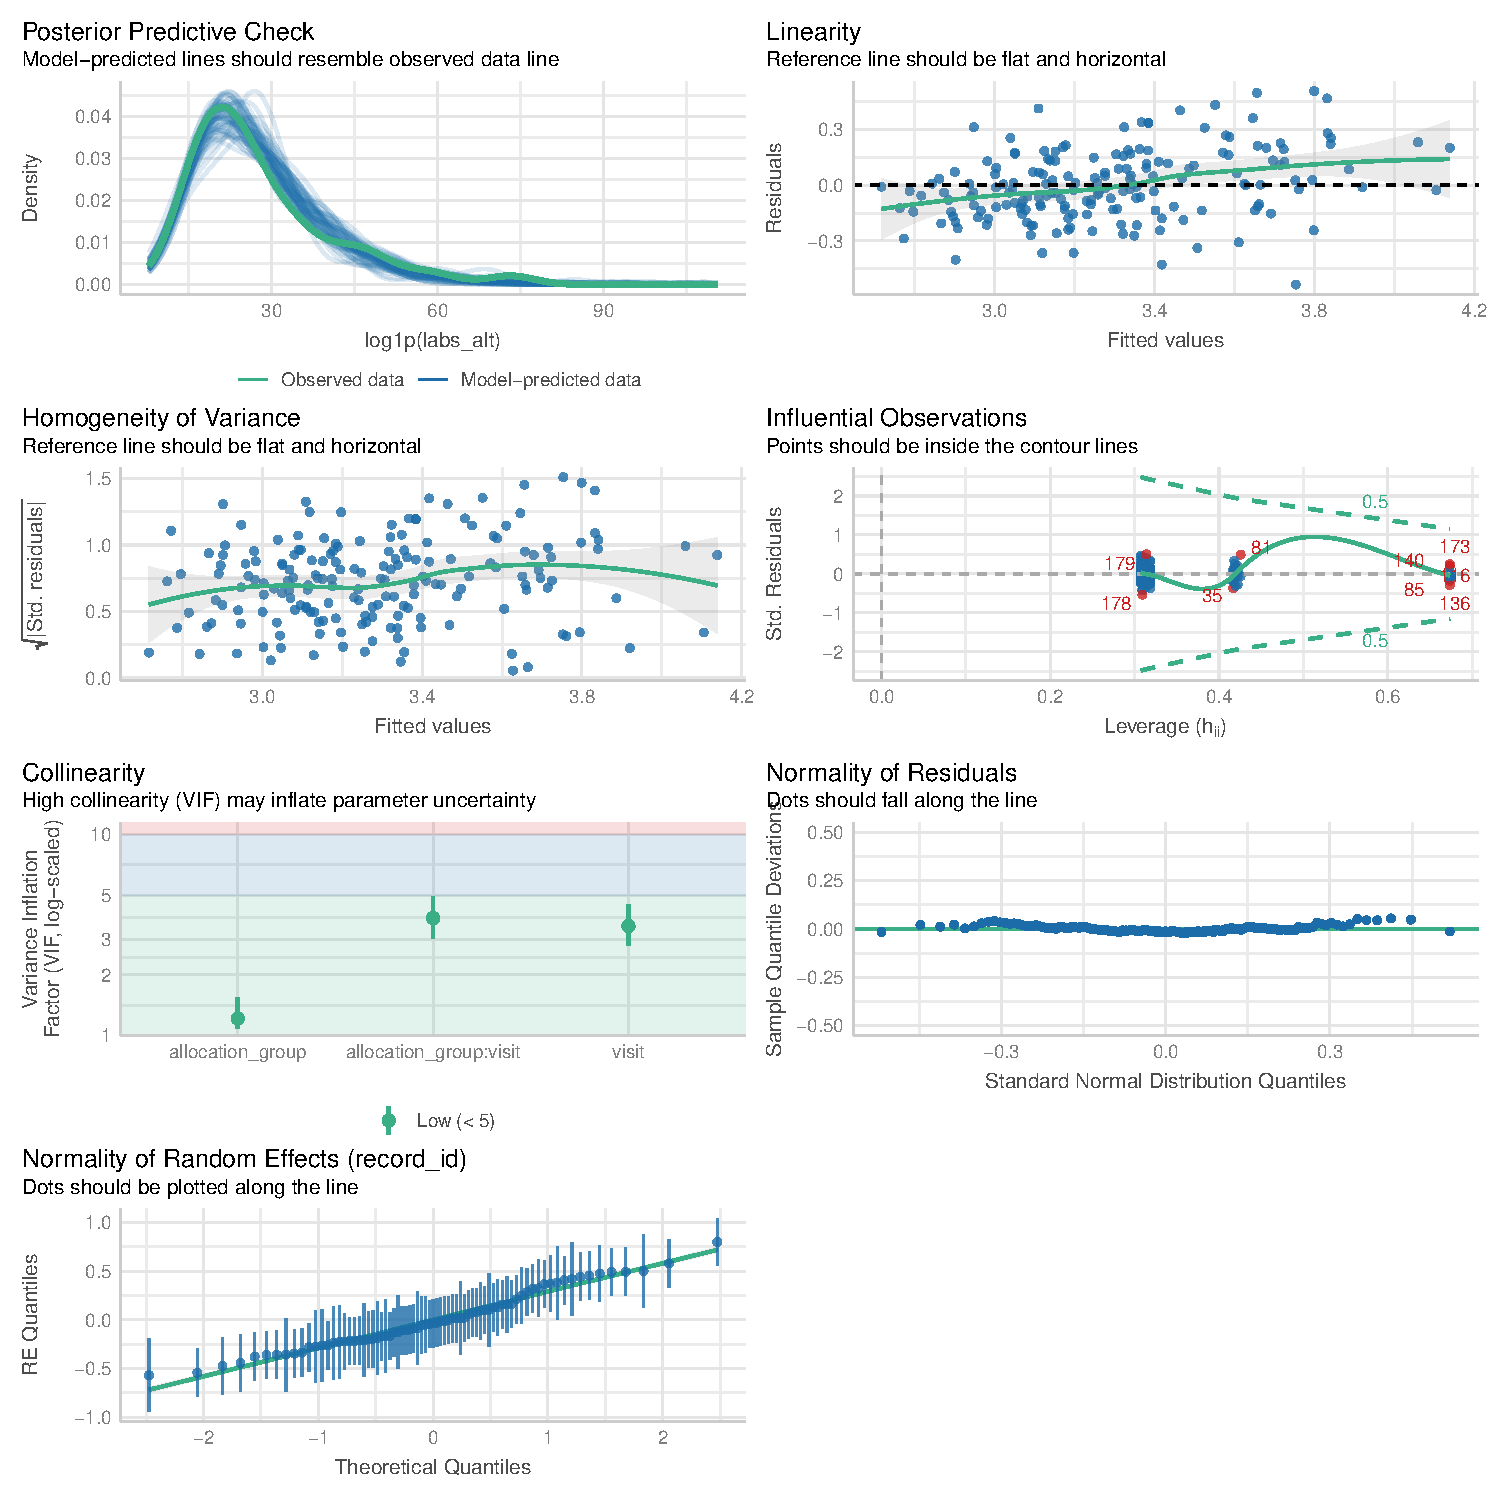
\includegraphics{Outcomes_V1V2V3_files/figure-pdf/labs_alt_4-1.pdf}

\begin{Shaded}
\begin{Highlighting}[]
\NormalTok{performance}\SpecialCharTok{::}\FunctionTok{check\_model}\NormalTok{(labs\_alt\_model\_sens)}
\end{Highlighting}
\end{Shaded}

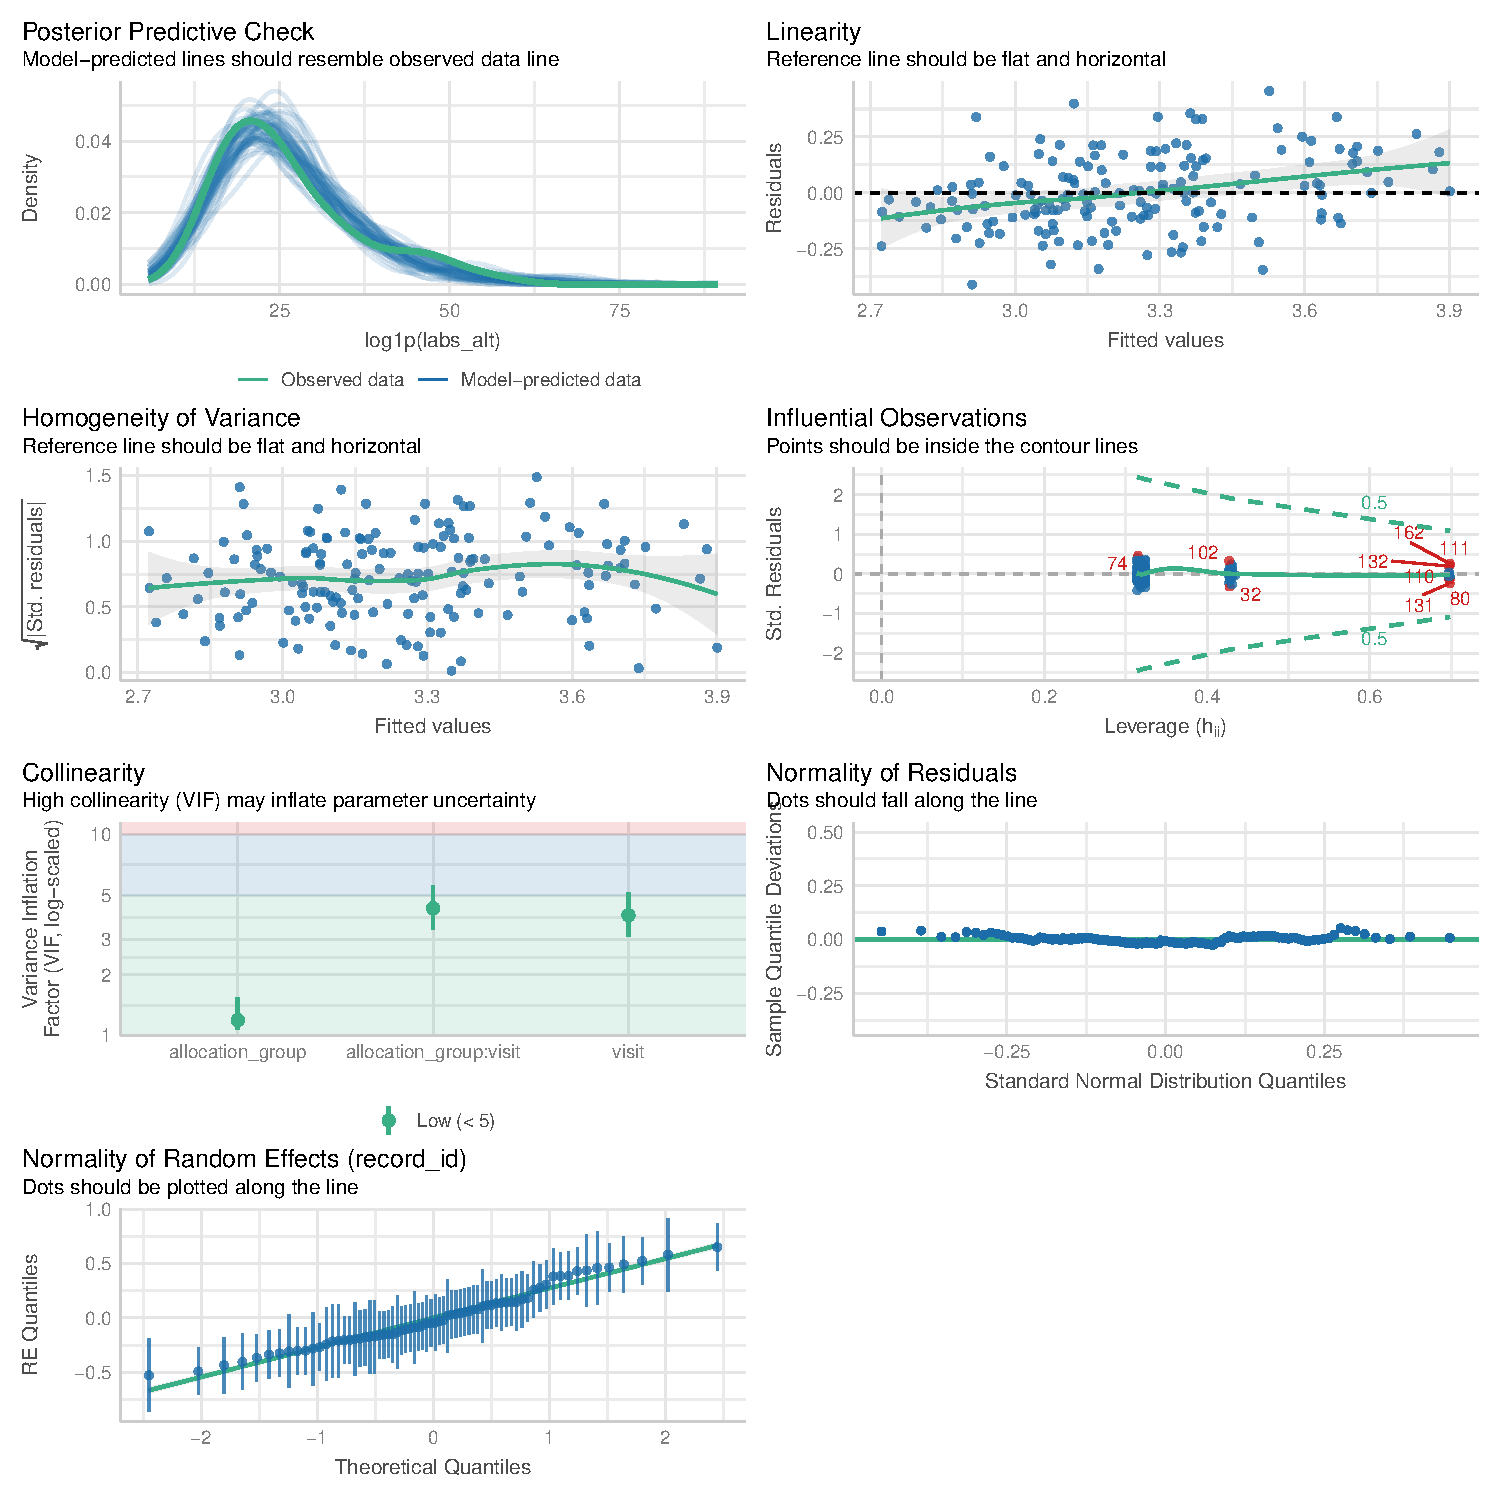
\includegraphics{Outcomes_V1V2V3_files/figure-pdf/labs_alt_4-2.pdf}

\paragraph{Médias Marginais
Estimadas}\label{muxe9dias-marginais-estimadas-1}

\begin{Shaded}
\begin{Highlighting}[]
\CommentTok{\# Get EMMs for each group at each visit}
\NormalTok{labs\_alt\_raw\_emm }\OtherTok{\textless{}{-}}\NormalTok{ emmeans}\SpecialCharTok{::}\FunctionTok{emmeans}\NormalTok{(}
\NormalTok{    labs\_alt\_model, }
    \SpecialCharTok{\textasciitilde{}}\NormalTok{ allocation\_group }\SpecialCharTok{*}\NormalTok{ visit}
\NormalTok{)}

\NormalTok{labs\_alt\_raw\_emm }\OtherTok{\textless{}{-}} \FunctionTok{regrid}\NormalTok{(labs\_alt\_raw\_emm)}

\CommentTok{\# Table of marginal means}
\NormalTok{labs\_alt\_raw\_emm}
\end{Highlighting}
\end{Shaded}

\begin{verbatim}
 allocation_group visit response   SE  df lower.CL upper.CL
 Grupo A          1         27.2 1.88 104     23.5     31.0
 Grupo B          1         24.5 1.67 104     21.2     27.8
 Grupo A          2         25.1 1.83 118     21.5     28.7
 Grupo B          2         24.0 1.84 134     20.4     27.7
 Grupo A          3         26.3 2.02 134     22.3     30.3
 Grupo B          3         25.7 2.05 146     21.6     29.7

Degrees-of-freedom method: inherited from kenward-roger when re-gridding 
Confidence level used: 0.95 
\end{verbatim}

\begin{Shaded}
\begin{Highlighting}[]
\CommentTok{\# Pairwise comparisons: Between groups at each visit}
\NormalTok{emmeans}\SpecialCharTok{::}\FunctionTok{contrast}\NormalTok{(labs\_alt\_raw\_emm, }\AttributeTok{method =} \StringTok{"pairwise"}\NormalTok{, }\AttributeTok{by =} \StringTok{"visit"}\NormalTok{, }\AttributeTok{adjust =} \StringTok{"bonferroni"}\NormalTok{) }\SpecialCharTok{\%\textgreater{}\%} \FunctionTok{summary}\NormalTok{(}\AttributeTok{infer =} \FunctionTok{c}\NormalTok{(}\ConstantTok{TRUE}\NormalTok{, }\ConstantTok{TRUE}\NormalTok{))}
\end{Highlighting}
\end{Shaded}

\begin{verbatim}
visit = 1:
 contrast          estimate   SE  df lower.CL upper.CL t.ratio p.value
 Grupo A - Grupo B    2.734 2.51 104    -2.25     7.72   1.088  0.2792

visit = 2:
 contrast          estimate   SE  df lower.CL upper.CL t.ratio p.value
 Grupo A - Grupo B    1.033 2.59 118    -4.10     6.16   0.399  0.6907

visit = 3:
 contrast          estimate   SE  df lower.CL upper.CL t.ratio p.value
 Grupo A - Grupo B    0.612 2.88 134    -5.09     6.32   0.212  0.8324

Degrees-of-freedom method: inherited from kenward-roger when re-gridding 
Confidence level used: 0.95 
\end{verbatim}

\begin{Shaded}
\begin{Highlighting}[]
\CommentTok{\# Pairwise comparisons: Changes over time within each group}
\NormalTok{emmeans}\SpecialCharTok{::}\FunctionTok{contrast}\NormalTok{(labs\_alt\_raw\_emm, }\AttributeTok{method =} \StringTok{"pairwise"}\NormalTok{, }\AttributeTok{by =} \StringTok{"allocation\_group"}\NormalTok{, }\AttributeTok{adjust =} \StringTok{"bonferroni"}\NormalTok{) }\SpecialCharTok{\%\textgreater{}\%} \FunctionTok{summary}\NormalTok{(}\AttributeTok{infer =} \FunctionTok{c}\NormalTok{(}\ConstantTok{TRUE}\NormalTok{, }\ConstantTok{TRUE}\NormalTok{))}
\end{Highlighting}
\end{Shaded}

\begin{verbatim}
allocation_group = Grupo A:
 contrast        estimate   SE  df lower.CL upper.CL t.ratio p.value
 visit1 - visit2    2.159 1.59 104    -1.71     6.03   1.357  0.5332
 visit1 - visit3    0.934 1.76 104    -3.35     5.21   0.531  1.0000
 visit2 - visit3   -1.225 1.72 118    -5.41     2.96  -0.711  1.0000

allocation_group = Grupo B:
 contrast        estimate   SE  df lower.CL upper.CL t.ratio p.value
 visit1 - visit2    0.458 1.59 104    -3.41     4.32   0.288  1.0000
 visit1 - visit3   -1.189 1.77 104    -5.49     3.11  -0.672  1.0000
 visit2 - visit3   -1.647 1.83 134    -6.07     2.78  -0.902  1.0000

Degrees-of-freedom method: inherited from kenward-roger when re-gridding 
Confidence level used: 0.95 
Conf-level adjustment: bonferroni method for 3 estimates 
P value adjustment: bonferroni method for 3 tests 
\end{verbatim}

\begin{Shaded}
\begin{Highlighting}[]
\CommentTok{\# Plot of marginal means}
\FunctionTok{plot}\NormalTok{(labs\_alt\_raw\_emm, }\AttributeTok{comparisons =} \ConstantTok{TRUE}\NormalTok{)}
\end{Highlighting}
\end{Shaded}

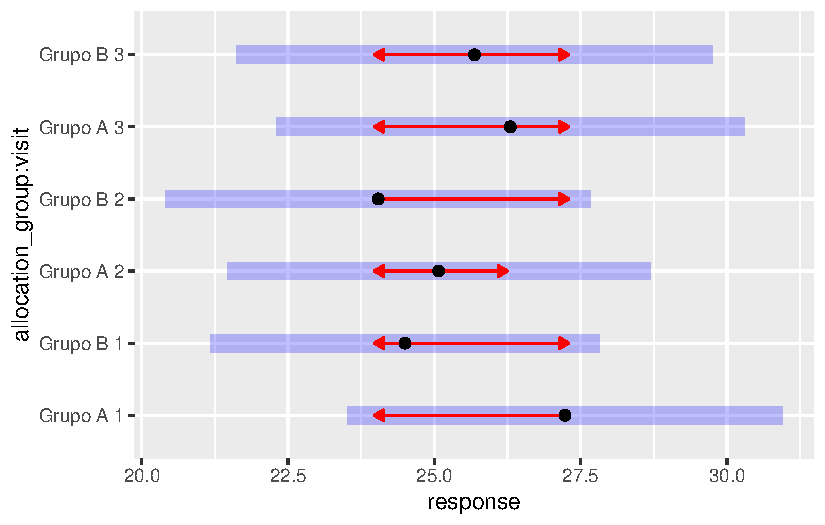
\includegraphics{Outcomes_V1V2V3_files/figure-pdf/labs_alt_raw_emm-1.pdf}

\begin{Shaded}
\begin{Highlighting}[]
\CommentTok{\# Get EMMs for each group at each visit}
\NormalTok{labs\_alt\_emm }\OtherTok{\textless{}{-}}\NormalTok{ emmeans}\SpecialCharTok{::}\FunctionTok{emmeans}\NormalTok{(}
\NormalTok{    labs\_alt\_model\_sens, }
    \SpecialCharTok{\textasciitilde{}}\NormalTok{ allocation\_group }\SpecialCharTok{*}\NormalTok{ visit}
\NormalTok{)}

\NormalTok{labs\_alt\_emm }\OtherTok{\textless{}{-}} \FunctionTok{regrid}\NormalTok{(labs\_alt\_emm)}

\CommentTok{\# Table of marginal means}
\NormalTok{labs\_alt\_emm}
\end{Highlighting}
\end{Shaded}

\begin{verbatim}
 allocation_group visit response   SE    df lower.CL upper.CL
 Grupo A          1         24.8 1.66  93.7     21.5     28.1
 Grupo B          1         24.5 1.54  93.7     21.4     27.5
 Grupo A          2         24.2 1.71 107.7     20.8     27.6
 Grupo B          2         23.7 1.65 118.5     20.4     27.0
 Grupo A          3         23.9 1.80 125.2     20.3     27.5
 Grupo B          3         24.7 1.82 133.0     21.1     28.3

Degrees-of-freedom method: inherited from kenward-roger when re-gridding 
Confidence level used: 0.95 
\end{verbatim}

\begin{Shaded}
\begin{Highlighting}[]
\CommentTok{\# Pairwise comparisons: Between groups at each visit}
\NormalTok{emmeans}\SpecialCharTok{::}\FunctionTok{contrast}\NormalTok{(labs\_alt\_emm, }\AttributeTok{method =} \StringTok{"pairwise"}\NormalTok{, }\AttributeTok{by =} \StringTok{"visit"}\NormalTok{, }\AttributeTok{adjust =} \StringTok{"bonferroni"}\NormalTok{) }\SpecialCharTok{\%\textgreater{}\%} \FunctionTok{summary}\NormalTok{(}\AttributeTok{infer =} \FunctionTok{c}\NormalTok{(}\ConstantTok{TRUE}\NormalTok{, }\ConstantTok{TRUE}\NormalTok{))}
\end{Highlighting}
\end{Shaded}

\begin{verbatim}
visit = 1:
 contrast          estimate   SE    df lower.CL upper.CL t.ratio p.value
 Grupo A - Grupo B    0.335 2.27  93.7    -4.16     4.83   0.148  0.8827

visit = 2:
 contrast          estimate   SE    df lower.CL upper.CL t.ratio p.value
 Grupo A - Grupo B    0.558 2.38 107.7    -4.17     5.28   0.234  0.8153

visit = 3:
 contrast          estimate   SE    df lower.CL upper.CL t.ratio p.value
 Grupo A - Grupo B   -0.770 2.56 125.2    -5.84     4.31  -0.300  0.7645

Degrees-of-freedom method: inherited from kenward-roger when re-gridding 
Confidence level used: 0.95 
\end{verbatim}

\begin{Shaded}
\begin{Highlighting}[]
\CommentTok{\# Pairwise comparisons: Changes over time within each group}
\NormalTok{emmeans}\SpecialCharTok{::}\FunctionTok{contrast}\NormalTok{(labs\_alt\_emm, }\AttributeTok{method =} \StringTok{"pairwise"}\NormalTok{, }\AttributeTok{by =} \StringTok{"allocation\_group"}\NormalTok{, }\AttributeTok{adjust =} \StringTok{"bonferroni"}\NormalTok{) }\SpecialCharTok{\%\textgreater{}\%} \FunctionTok{summary}\NormalTok{(}\AttributeTok{infer =} \FunctionTok{c}\NormalTok{(}\ConstantTok{TRUE}\NormalTok{, }\ConstantTok{TRUE}\NormalTok{))}
\end{Highlighting}
\end{Shaded}

\begin{verbatim}
allocation_group = Grupo A:
 contrast        estimate   SE    df lower.CL upper.CL t.ratio p.value
 visit1 - visit2    0.549 1.41  93.7    -2.88     3.98   0.390  1.0000
 visit1 - visit3    0.897 1.53  93.7    -2.84     4.63   0.586  1.0000
 visit2 - visit3    0.348 1.54 107.7    -3.39     4.09   0.226  1.0000

allocation_group = Grupo B:
 contrast        estimate   SE    df lower.CL upper.CL t.ratio p.value
 visit1 - visit2    0.772 1.39  93.7    -2.62     4.16   0.555  1.0000
 visit1 - visit3   -0.207 1.55  93.7    -3.98     3.56  -0.134  1.0000
 visit2 - visit3   -0.980 1.57 118.5    -4.80     2.84  -0.622  1.0000

Degrees-of-freedom method: inherited from kenward-roger when re-gridding 
Confidence level used: 0.95 
Conf-level adjustment: bonferroni method for 3 estimates 
P value adjustment: bonferroni method for 3 tests 
\end{verbatim}

\begin{Shaded}
\begin{Highlighting}[]
\CommentTok{\# Plot of marginal means}
\FunctionTok{plot}\NormalTok{(labs\_alt\_emm, }\AttributeTok{comparisons =} \ConstantTok{TRUE}\NormalTok{)}
\end{Highlighting}
\end{Shaded}

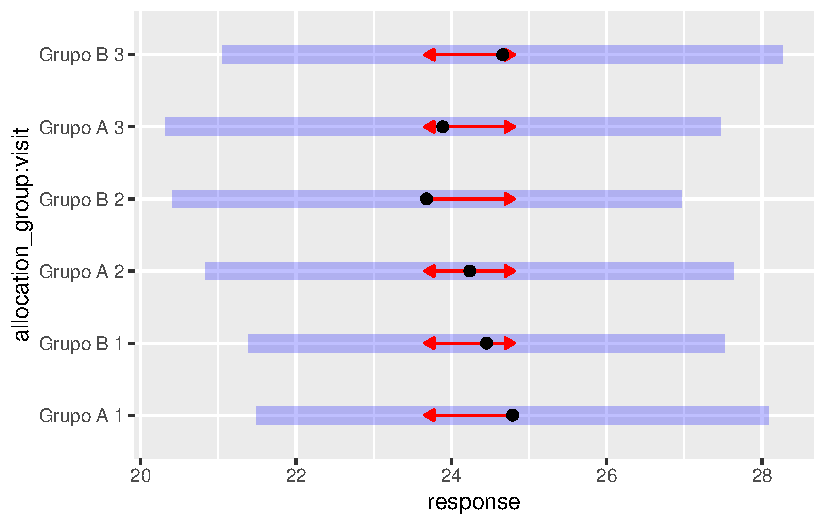
\includegraphics{Outcomes_V1V2V3_files/figure-pdf/labs_alt_sens_emm-1.pdf}

\begin{Shaded}
\begin{Highlighting}[]
\FunctionTok{ggplot}\NormalTok{(}
    \AttributeTok{data =}\NormalTok{ data\_model, }
    \FunctionTok{aes}\NormalTok{(}
        \AttributeTok{x =} \FunctionTok{as.factor}\NormalTok{(visit),}
        \AttributeTok{y =}\NormalTok{ labs\_alt,}
        \AttributeTok{group =}\NormalTok{ record\_id,}
\NormalTok{    )}
\NormalTok{) }\SpecialCharTok{+}
    \FunctionTok{geom\_line}\NormalTok{(}\AttributeTok{alpha =} \FloatTok{0.5}\NormalTok{) }\SpecialCharTok{+}
    \FunctionTok{geom\_point}\NormalTok{(}\AttributeTok{alpha =} \FloatTok{0.7}\NormalTok{) }\SpecialCharTok{+}
    \FunctionTok{geom\_smooth}\NormalTok{(}
        \FunctionTok{aes}\NormalTok{(}\AttributeTok{group =}\NormalTok{ allocation\_group),}
        \AttributeTok{method =} \StringTok{"lm"}\NormalTok{,}
        \AttributeTok{se =} \ConstantTok{TRUE}\NormalTok{,}
        \AttributeTok{linewidth =} \DecValTok{1}
\NormalTok{    ) }\SpecialCharTok{+}
    \FunctionTok{labs}\NormalTok{(}\AttributeTok{title =} \StringTok{"All data"}\NormalTok{) }\SpecialCharTok{+}
    \FunctionTok{facet\_wrap}\NormalTok{(}\SpecialCharTok{\textasciitilde{}}\NormalTok{ allocation\_group) }\SpecialCharTok{+} 
    \FunctionTok{coord\_cartesian}\NormalTok{(}\AttributeTok{ylim =} \FunctionTok{c}\NormalTok{(}\DecValTok{10}\NormalTok{, }\DecValTok{80}\NormalTok{))}
\end{Highlighting}
\end{Shaded}

\begin{verbatim}
`geom_smooth()` using formula = 'y ~ x'
\end{verbatim}

\begin{verbatim}
Warning: Removed 10 rows containing non-finite outside the scale range
(`stat_smooth()`).
\end{verbatim}

\begin{verbatim}
Warning: Removed 8 rows containing missing values or values outside the scale range
(`geom_line()`).
\end{verbatim}

\begin{verbatim}
Warning: Removed 10 rows containing missing values or values outside the scale range
(`geom_point()`).
\end{verbatim}

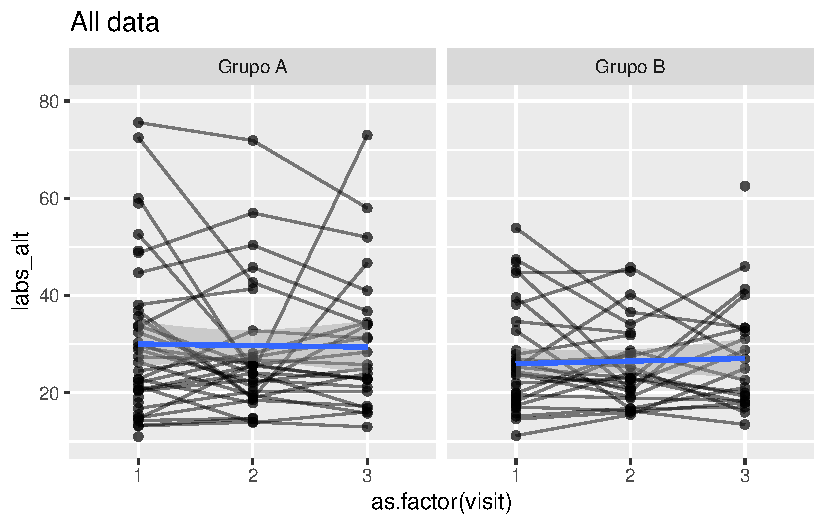
\includegraphics{Outcomes_V1V2V3_files/figure-pdf/labs_alt_6-1.pdf}

\begin{Shaded}
\begin{Highlighting}[]
\NormalTok{data\_model }\SpecialCharTok{\%\textgreater{}\%} 
    \FunctionTok{filter}\NormalTok{(}
        \SpecialCharTok{!}\NormalTok{(record\_id }\SpecialCharTok{\%in\%}\NormalTok{ labs\_alt\_model\_check}\SpecialCharTok{$}\NormalTok{influential\_ids)}
\NormalTok{    ) }\SpecialCharTok{\%\textgreater{}\%} 
    \FunctionTok{ggplot}\NormalTok{(}
        \FunctionTok{aes}\NormalTok{(}
            \AttributeTok{x =} \FunctionTok{as.factor}\NormalTok{(visit),}
            \AttributeTok{y =}\NormalTok{ labs\_alt,}
            \AttributeTok{group =}\NormalTok{ record\_id,}
\NormalTok{        )}
\NormalTok{    ) }\SpecialCharTok{+}
    \FunctionTok{geom\_line}\NormalTok{(}\AttributeTok{alpha =} \FloatTok{0.5}\NormalTok{) }\SpecialCharTok{+}
    \FunctionTok{geom\_point}\NormalTok{(}\AttributeTok{alpha =} \FloatTok{0.7}\NormalTok{) }\SpecialCharTok{+}
    \FunctionTok{geom\_smooth}\NormalTok{(}
        \FunctionTok{aes}\NormalTok{(}\AttributeTok{group =}\NormalTok{ allocation\_group),}
        \AttributeTok{method =} \StringTok{"lm"}\NormalTok{,}
        \AttributeTok{se =} \ConstantTok{TRUE}\NormalTok{,}
        \AttributeTok{linewidth =} \DecValTok{1}
\NormalTok{    ) }\SpecialCharTok{+}
    \FunctionTok{labs}\NormalTok{(}\AttributeTok{title =} \StringTok{"Sensitivity analysis"}\NormalTok{) }\SpecialCharTok{+}
    \FunctionTok{facet\_wrap}\NormalTok{(}\SpecialCharTok{\textasciitilde{}}\NormalTok{ allocation\_group) }\SpecialCharTok{+} 
    \FunctionTok{coord\_cartesian}\NormalTok{(}\AttributeTok{ylim =} \FunctionTok{c}\NormalTok{(}\DecValTok{10}\NormalTok{, }\DecValTok{80}\NormalTok{))}
\end{Highlighting}
\end{Shaded}

\begin{verbatim}
`geom_smooth()` using formula = 'y ~ x'
\end{verbatim}

\begin{verbatim}
Warning: Removed 9 rows containing non-finite outside the scale range
(`stat_smooth()`).
\end{verbatim}

\begin{verbatim}
Warning: Removed 8 rows containing missing values or values outside the scale range
(`geom_line()`).
\end{verbatim}

\begin{verbatim}
Warning: Removed 9 rows containing missing values or values outside the scale range
(`geom_point()`).
\end{verbatim}

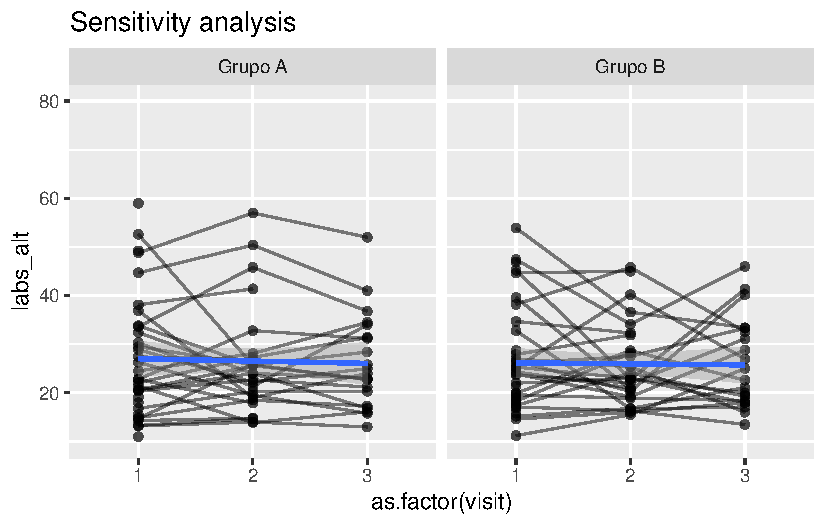
\includegraphics{Outcomes_V1V2V3_files/figure-pdf/labs_alt_6-2.pdf}

\subsubsection{Gama
Glutamil-transferase}\label{gama-glutamil-transferase}

Variável: \texttt{labs\_ggt}

\begin{Shaded}
\begin{Highlighting}[]
\CommentTok{\# Plot 1: Raw data}
\NormalTok{labs\_ggt\_hist\_1 }\OtherTok{\textless{}{-}}\NormalTok{ data\_model }\SpecialCharTok{\%\textgreater{}\%} 
    \FunctionTok{filter}\NormalTok{(}
\NormalTok{        labs\_ggt }\SpecialCharTok{\textless{}} \DecValTok{300}
\NormalTok{    ) }\SpecialCharTok{\%\textgreater{}\%} 
    \FunctionTok{ggplot}\NormalTok{(}\FunctionTok{aes}\NormalTok{(}\AttributeTok{x =}\NormalTok{ labs\_ggt)) }\SpecialCharTok{+} 
    \FunctionTok{geom\_histogram}\NormalTok{(}\AttributeTok{bins =} \DecValTok{50}\NormalTok{, }\AttributeTok{fill =} \StringTok{"skyblue"}\NormalTok{, }\AttributeTok{color =} \StringTok{"black"}\NormalTok{)}

\CommentTok{\# Plot 2: Log{-}transformed data}
\NormalTok{labs\_ggt\_hist\_2 }\OtherTok{\textless{}{-}}\NormalTok{ data\_model }\SpecialCharTok{\%\textgreater{}\%} 
    \FunctionTok{filter}\NormalTok{(}
\NormalTok{        labs\_ggt }\SpecialCharTok{\textless{}} \DecValTok{300}
\NormalTok{    ) }\SpecialCharTok{\%\textgreater{}\%}
    \FunctionTok{ggplot}\NormalTok{(}\FunctionTok{aes}\NormalTok{(}\AttributeTok{x =} \FunctionTok{log1p}\NormalTok{(labs\_ggt))) }\SpecialCharTok{+} 
    \FunctionTok{geom\_histogram}\NormalTok{(}\AttributeTok{bins =} \DecValTok{50}\NormalTok{, }\AttributeTok{fill =} \StringTok{"lightgreen"}\NormalTok{, }\AttributeTok{color =} \StringTok{"black"}\NormalTok{)}

\CommentTok{\# Combine side by side}
\NormalTok{labs\_ggt\_hist\_1 }\SpecialCharTok{+}\NormalTok{ labs\_ggt\_hist\_2 }\CommentTok{\# library(patchwork)}
\end{Highlighting}
\end{Shaded}

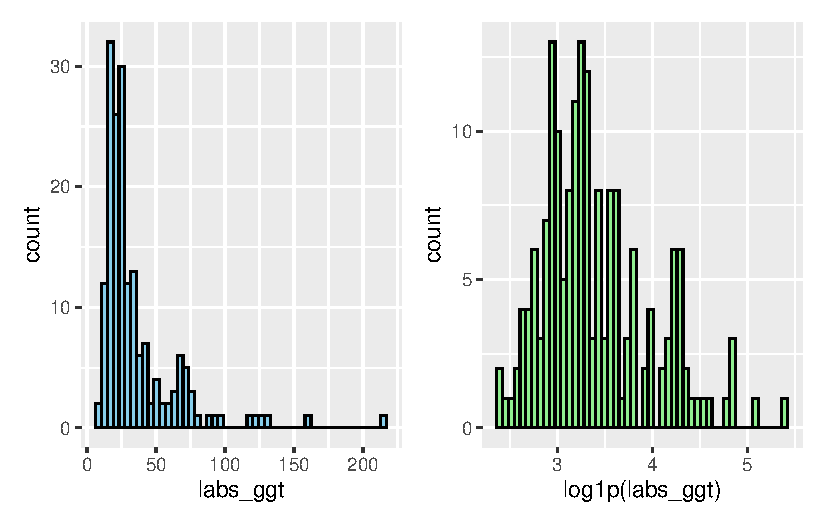
\includegraphics{Outcomes_V1V2V3_files/figure-pdf/labs_ggt_1-1.pdf}

\begin{Shaded}
\begin{Highlighting}[]
\CommentTok{\# LMM}
\NormalTok{labs\_ggt\_model }\OtherTok{\textless{}{-}} \FunctionTok{lmer}\NormalTok{(}\FunctionTok{log1p}\NormalTok{(labs\_ggt) }\SpecialCharTok{\textasciitilde{}}\NormalTok{ allocation\_group }\SpecialCharTok{*}\NormalTok{ visit }\SpecialCharTok{+}\NormalTok{ (}\DecValTok{1} \SpecialCharTok{|}\NormalTok{ record\_id), }\AttributeTok{data =}\NormalTok{ data\_model)}
\FunctionTok{check\_collinearity}\NormalTok{(labs\_ggt\_model)}
\end{Highlighting}
\end{Shaded}

\begin{verbatim}
# Check for Multicollinearity

Low Correlation

                   Term  VIF   VIF 95% CI Increased SE Tolerance
       allocation_group 1.08 [1.01, 1.64]         1.04      0.93
                  visit 3.40 [2.71, 4.36]         1.84      0.29
 allocation_group:visit 3.51 [2.79, 4.51]         1.87      0.28
 Tolerance 95% CI
     [0.61, 0.99]
     [0.23, 0.37]
     [0.22, 0.36]
\end{verbatim}

\begin{Shaded}
\begin{Highlighting}[]
\CommentTok{\# Sensitivity analysis}
\NormalTok{labs\_ggt\_model\_check }\OtherTok{\textless{}{-}} \FunctionTok{sensitivity\_check\_lmer}\NormalTok{(}
    \AttributeTok{model =}\NormalTok{ labs\_ggt\_model,}
    \AttributeTok{id\_var =} \StringTok{"record\_id"}\NormalTok{,}
    \AttributeTok{top\_n =} \DecValTok{7}\NormalTok{)}

\CommentTok{\# LMM Sensitivity}
\NormalTok{labs\_ggt\_model\_sens }\OtherTok{\textless{}{-}} \FunctionTok{update}\NormalTok{(}\AttributeTok{object =}\NormalTok{ labs\_ggt\_model,}
                              \AttributeTok{subset =} \SpecialCharTok{!}\NormalTok{(record\_id }\SpecialCharTok{\%in\%}\NormalTok{ labs\_ggt\_model\_check}\SpecialCharTok{$}\NormalTok{influential\_ids))}
\CommentTok{\# Influential IDS}
\NormalTok{labs\_ggt\_model\_check}\SpecialCharTok{$}\NormalTok{influential\_ids}
\end{Highlighting}
\end{Shaded}

\begin{verbatim}
[1] "13" "46" "49" "58" "22" "34" "41"
\end{verbatim}

\paragraph{Resumo dos modelos}\label{resumo-dos-modelos-2}

\begin{Shaded}
\begin{Highlighting}[]
\CommentTok{\# Model comparison}
\FunctionTok{summary}\NormalTok{(labs\_ggt\_model)}
\end{Highlighting}
\end{Shaded}

\begin{verbatim}
Linear mixed model fit by REML. t-tests use Satterthwaite's method [
lmerModLmerTest]
Formula: log1p(labs_ggt) ~ allocation_group * visit + (1 | record_id)
   Data: data_model

REML criterion at convergence: 214.3

Scaled residuals: 
     Min       1Q   Median       3Q      Max 
-1.98517 -0.41941 -0.02504  0.42332  2.68048 

Random effects:
 Groups    Name        Variance Std.Dev.
 record_id (Intercept) 0.35840  0.5987  
 Residual              0.05825  0.2413  
Number of obs: 178, groups:  record_id, 75

Fixed effects:
                               Estimate Std. Error       df t value Pr(>|t|)
(Intercept)                     3.36365    0.10612 81.55575  31.697   <2e-16
allocation_groupGrupo B         0.05279    0.14908 81.55575   0.354    0.724
visit2                         -0.02673    0.06095 98.79849  -0.439    0.662
visit3                          0.01219    0.06614 99.26017   0.184    0.854
allocation_groupGrupo B:visit2  0.04689    0.08964 99.59537   0.523    0.602
allocation_groupGrupo B:visit3  0.02698    0.09736 99.95801   0.277    0.782
                                  
(Intercept)                    ***
allocation_groupGrupo B           
visit2                            
visit3                            
allocation_groupGrupo B:visit2    
allocation_groupGrupo B:visit3    
---
Signif. codes:  0 '***' 0.001 '**' 0.01 '*' 0.05 '.' 0.1 ' ' 1

Correlation of Fixed Effects:
            (Intr) all_GB visit2 visit3 a_GB:2
allctn_grGB -0.712                            
visit2      -0.243  0.173                     
visit3      -0.224  0.160  0.455              
allctn_GB:2  0.166 -0.233 -0.680 -0.310       
allctn_GB:3  0.152 -0.214 -0.309 -0.679  0.436
\end{verbatim}

\begin{Shaded}
\begin{Highlighting}[]
\FunctionTok{summary}\NormalTok{(labs\_ggt\_model\_sens)}
\end{Highlighting}
\end{Shaded}

\begin{verbatim}
Linear mixed model fit by REML. t-tests use Satterthwaite's method [
lmerModLmerTest]
Formula: log1p(labs_ggt) ~ allocation_group * visit + (1 | record_id)
   Data: data_model
 Subset: !(record_id %in% labs_ggt_model_check$influential_ids)

REML criterion at convergence: 129.2

Scaled residuals: 
     Min       1Q   Median       3Q      Max 
-2.06521 -0.44956 -0.01804  0.45494  1.81501 

Random effects:
 Groups    Name        Variance Std.Dev.
 record_id (Intercept) 0.2520   0.5020  
 Residual              0.0364   0.1908  
Number of obs: 160, groups:  record_id, 68

Fixed effects:
                               Estimate Std. Error       df t value Pr(>|t|)
(Intercept)                     3.21202    0.09349 74.25204  34.357   <2e-16
allocation_groupGrupo B         0.14499    0.13031 74.25204   1.113    0.269
visit2                         -0.01105    0.05075 89.14440  -0.218    0.828
visit3                          0.03893    0.05564 89.56439   0.700    0.486
allocation_groupGrupo B:visit2  0.06129    0.07498 89.97944   0.817    0.416
allocation_groupGrupo B:visit3  0.01693    0.08145 90.24696   0.208    0.836
                                  
(Intercept)                    ***
allocation_groupGrupo B           
visit2                            
visit3                            
allocation_groupGrupo B:visit2    
allocation_groupGrupo B:visit3    
---
Signif. codes:  0 '***' 0.001 '**' 0.01 '*' 0.05 '.' 0.1 ' ' 1

Correlation of Fixed Effects:
            (Intr) all_GB visit2 visit3 a_GB:2
allctn_grGB -0.717                            
visit2      -0.233  0.167                     
visit3      -0.212  0.152  0.452              
allctn_GB:2  0.157 -0.219 -0.677 -0.306       
allctn_GB:3  0.145 -0.202 -0.309 -0.683  0.434
\end{verbatim}

\begin{Shaded}
\begin{Highlighting}[]
\NormalTok{labs\_ggt\_model\_check}\SpecialCharTok{$}\NormalTok{comparison\_table}
\end{Highlighting}
\end{Shaded}

\begin{verbatim}
# A tibble: 16 x 6
   Model       term                       estimate std.error statistic   p.value
   <chr>       <chr>                         <dbl>     <dbl>     <dbl>     <dbl>
 1 Original    (Intercept)                  3.36      0.106     31.7    1.28e-47
 2 Sensitivity (Intercept)                  3.21      0.0935    34.4    2.48e-47
 3 Original    allocation_groupGrupo B      0.0528    0.149      0.354  7.24e- 1
 4 Sensitivity allocation_groupGrupo B      0.145     0.130      1.11   2.69e- 1
 5 Original    allocation_groupGrupo B:v~   0.0469    0.0896     0.523  6.02e- 1
 6 Sensitivity allocation_groupGrupo B:v~   0.0613    0.0750     0.817  4.16e- 1
 7 Original    allocation_groupGrupo B:v~   0.0270    0.0974     0.277  7.82e- 1
 8 Sensitivity allocation_groupGrupo B:v~   0.0169    0.0814     0.208  8.36e- 1
 9 Original    sd__(Intercept)              0.599    NA         NA     NA       
10 Sensitivity sd__(Intercept)              0.502    NA         NA     NA       
11 Original    sd__Observation              0.241    NA         NA     NA       
12 Sensitivity sd__Observation              0.191    NA         NA     NA       
13 Original    visit2                      -0.0267    0.0610    -0.439  6.62e- 1
14 Sensitivity visit2                      -0.0110    0.0507    -0.218  8.28e- 1
15 Original    visit3                       0.0122    0.0661     0.184  8.54e- 1
16 Sensitivity visit3                       0.0389    0.0556     0.700  4.86e- 1
\end{verbatim}

\begin{Shaded}
\begin{Highlighting}[]
\NormalTok{performance}\SpecialCharTok{::}\FunctionTok{compare\_performance}\NormalTok{(labs\_ggt\_model, labs\_ggt\_model\_sens)}
\end{Highlighting}
\end{Shaded}

\begin{verbatim}
When comparing models, please note that probably not all models were fit
  from same data.
\end{verbatim}

\begin{verbatim}
# Comparison of Model Performance Indices

Name                |           Model |  AIC (weights) | AICc (weights)
-----------------------------------------------------------------------
labs_ggt_model      | lmerModLmerTest | 1425.1 (<.001) | 1426.0 (<.001)
labs_ggt_model_sens | lmerModLmerTest | 1189.5 (>.999) | 1190.4 (>.999)

Name                |  BIC (weights) | R2 (cond.) | R2 (marg.) |   ICC |  RMSE | Sigma
--------------------------------------------------------------------------------------
labs_ggt_model      | 1450.6 (<.001) |      0.861 |      0.004 | 0.860 | 0.185 | 0.241
labs_ggt_model_sens | 1214.1 (>.999) |      0.877 |      0.026 | 0.874 | 0.145 | 0.191
\end{verbatim}

\begin{Shaded}
\begin{Highlighting}[]
\NormalTok{performance}\SpecialCharTok{::}\FunctionTok{check\_model}\NormalTok{(labs\_ggt\_model)}
\end{Highlighting}
\end{Shaded}

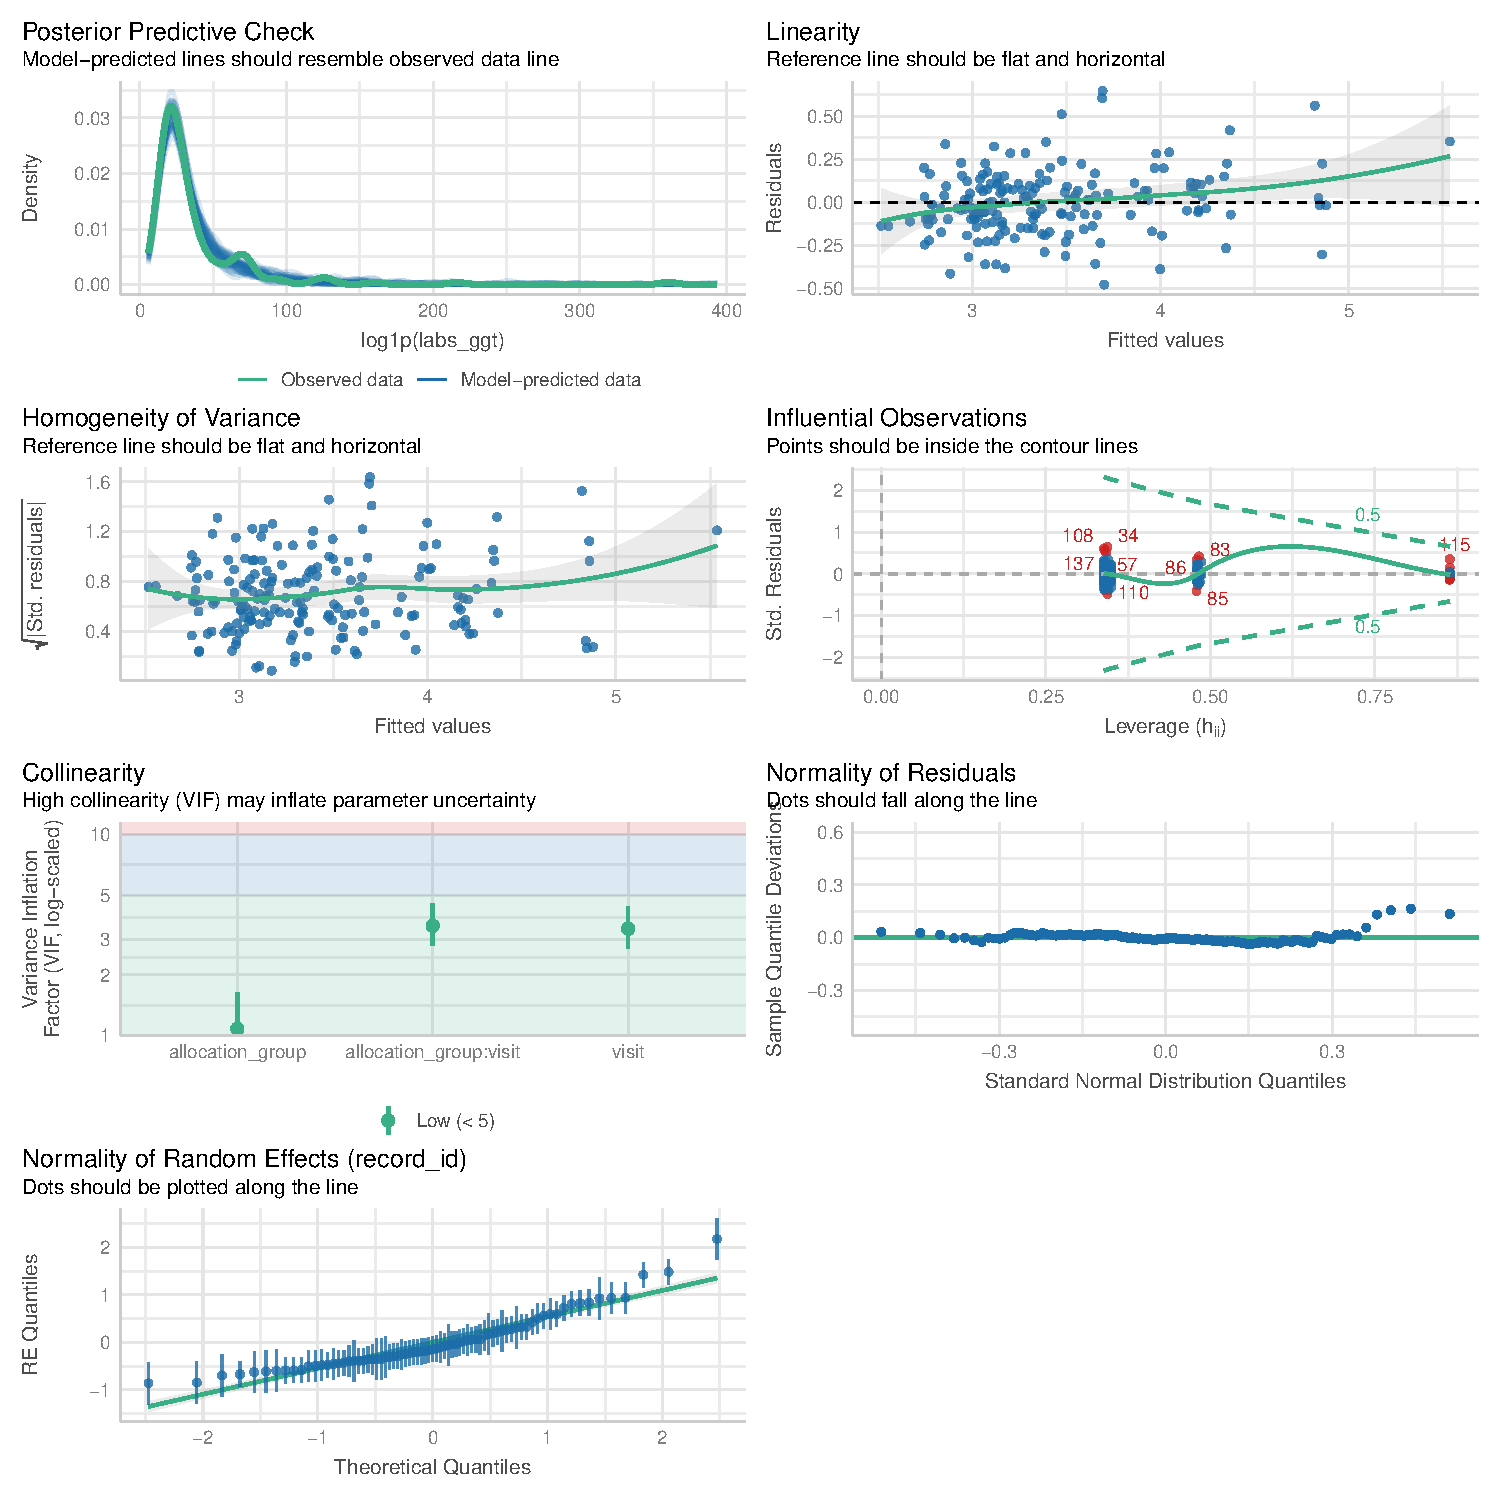
\includegraphics{Outcomes_V1V2V3_files/figure-pdf/labs_ggt_4-1.pdf}

\begin{Shaded}
\begin{Highlighting}[]
\NormalTok{performance}\SpecialCharTok{::}\FunctionTok{check\_model}\NormalTok{(labs\_ggt\_model\_sens)}
\end{Highlighting}
\end{Shaded}

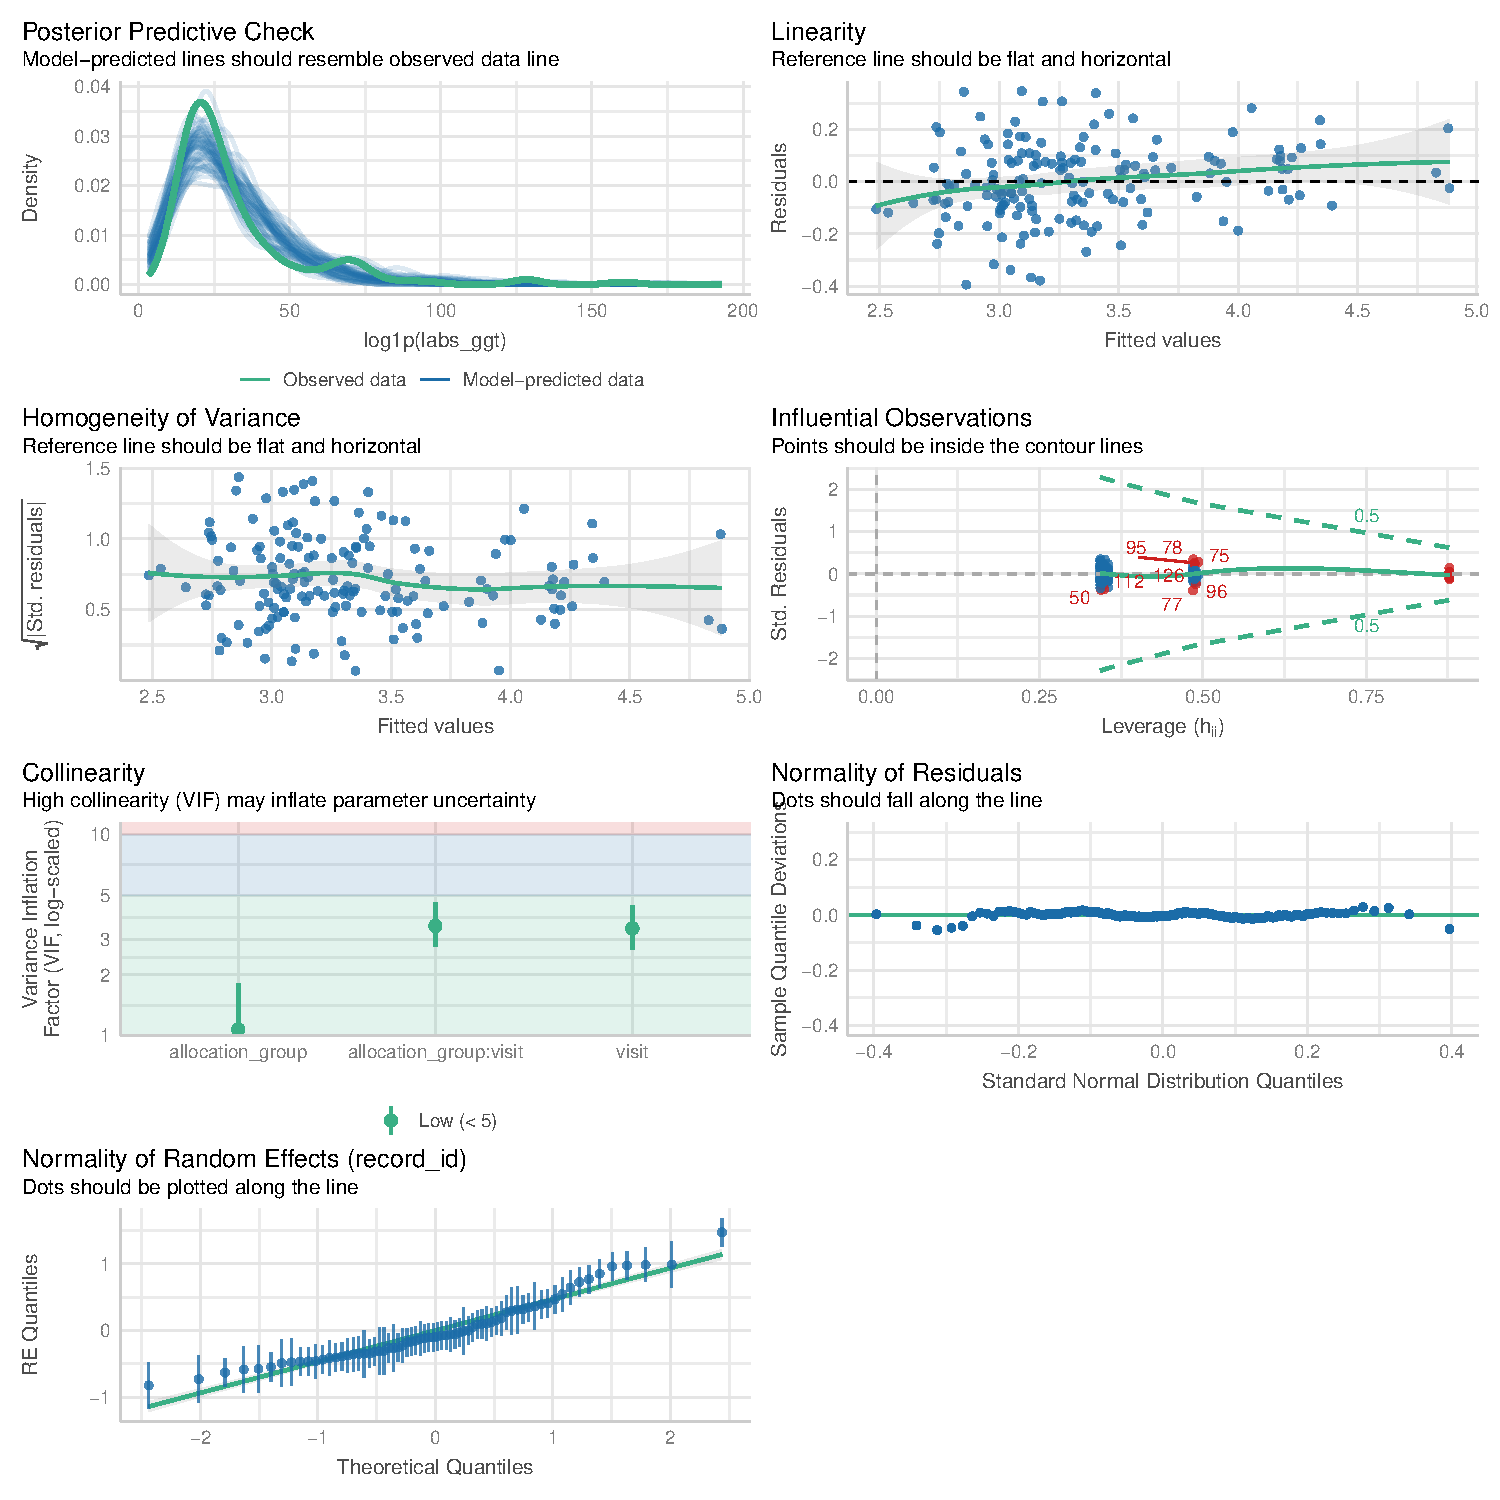
\includegraphics{Outcomes_V1V2V3_files/figure-pdf/labs_ggt_4-2.pdf}

\paragraph{Médias Marginais
Estimadas}\label{muxe9dias-marginais-estimadas-2}

\begin{Shaded}
\begin{Highlighting}[]
\CommentTok{\# Get EMMs for each group at each visit}
\NormalTok{labs\_ggt\_raw\_emm }\OtherTok{\textless{}{-}}\NormalTok{ emmeans}\SpecialCharTok{::}\FunctionTok{emmeans}\NormalTok{(}
\NormalTok{    labs\_ggt\_model, }
    \SpecialCharTok{\textasciitilde{}}\NormalTok{ allocation\_group }\SpecialCharTok{*}\NormalTok{ visit}
\NormalTok{)}

\NormalTok{labs\_ggt\_raw\_emm }\OtherTok{\textless{}{-}} \FunctionTok{regrid}\NormalTok{(labs\_ggt\_raw\_emm)}

\CommentTok{\# Table of marginal means}
\NormalTok{labs\_ggt\_raw\_emm}
\end{Highlighting}
\end{Shaded}

\begin{verbatim}
 allocation_group visit response   SE    df lower.CL upper.CL
 Grupo A          1         27.9 3.07  84.1     21.8     34.0
 Grupo B          1         29.5 3.19  84.1     23.1     35.8
 Grupo A          2         27.1 3.06  91.4     21.1     33.2
 Grupo B          2         30.1 3.44 100.6     23.3     36.9
 Grupo A          3         28.2 3.27 100.1     21.8     34.7
 Grupo B          3         30.7 3.61 110.8     23.5     37.8

Degrees-of-freedom method: inherited from kenward-roger when re-gridding 
Confidence level used: 0.95 
\end{verbatim}

\begin{Shaded}
\begin{Highlighting}[]
\CommentTok{\# Pairwise comparisons: Between groups at each visit}
\NormalTok{emmeans}\SpecialCharTok{::}\FunctionTok{contrast}\NormalTok{(labs\_ggt\_raw\_emm, }\AttributeTok{method =} \StringTok{"pairwise"}\NormalTok{, }\AttributeTok{by =} \StringTok{"visit"}\NormalTok{, }\AttributeTok{adjust =} \StringTok{"bonferroni"}\NormalTok{) }\SpecialCharTok{\%\textgreater{}\%} \FunctionTok{summary}\NormalTok{(}\AttributeTok{infer =} \FunctionTok{c}\NormalTok{(}\ConstantTok{TRUE}\NormalTok{, }\ConstantTok{TRUE}\NormalTok{))}
\end{Highlighting}
\end{Shaded}

\begin{verbatim}
visit = 1:
 contrast          estimate   SE    df lower.CL upper.CL t.ratio p.value
 Grupo A - Grupo B    -1.57 4.42  84.1    -10.4     7.23  -0.354  0.7242

visit = 2:
 contrast          estimate   SE    df lower.CL upper.CL t.ratio p.value
 Grupo A - Grupo B    -2.95 4.60  91.4    -12.1     6.19  -0.641  0.5232

visit = 3:
 contrast          estimate   SE    df lower.CL upper.CL t.ratio p.value
 Grupo A - Grupo B    -2.43 4.87 100.1    -12.1     7.24  -0.498  0.6193

Degrees-of-freedom method: inherited from kenward-roger when re-gridding 
Confidence level used: 0.95 
\end{verbatim}

\begin{Shaded}
\begin{Highlighting}[]
\CommentTok{\# Pairwise comparisons: Changes over time within each group}
\NormalTok{emmeans}\SpecialCharTok{::}\FunctionTok{contrast}\NormalTok{(labs\_ggt\_raw\_emm, }\AttributeTok{method =} \StringTok{"pairwise"}\NormalTok{, }\AttributeTok{by =} \StringTok{"allocation\_group"}\NormalTok{, }\AttributeTok{adjust =} \StringTok{"bonferroni"}\NormalTok{) }\SpecialCharTok{\%\textgreater{}\%} \FunctionTok{summary}\NormalTok{(}\AttributeTok{infer =} \FunctionTok{c}\NormalTok{(}\ConstantTok{TRUE}\NormalTok{, }\ConstantTok{TRUE}\NormalTok{))}
\end{Highlighting}
\end{Shaded}

\begin{verbatim}
allocation_group = Grupo A:
 contrast        estimate   SE    df lower.CL upper.CL t.ratio p.value
 visit1 - visit2    0.762 1.74  84.1    -3.48     5.01   0.439  1.0000
 visit1 - visit3   -0.354 1.93  84.1    -5.06     4.35  -0.184  1.0000
 visit2 - visit3   -1.116 1.92  91.4    -5.79     3.56  -0.583  1.0000

allocation_group = Grupo B:
 contrast        estimate   SE    df lower.CL upper.CL t.ratio p.value
 visit1 - visit2   -0.620 2.03  84.1    -5.58     4.34  -0.305  1.0000
 visit1 - visit3   -1.217 2.24  84.1    -6.69     4.26  -0.543  1.0000
 visit2 - visit3   -0.596 2.33 100.6    -6.27     5.08  -0.256  1.0000

Degrees-of-freedom method: inherited from kenward-roger when re-gridding 
Confidence level used: 0.95 
Conf-level adjustment: bonferroni method for 3 estimates 
P value adjustment: bonferroni method for 3 tests 
\end{verbatim}

\begin{Shaded}
\begin{Highlighting}[]
\CommentTok{\# Plot of marginal means}
\FunctionTok{plot}\NormalTok{(labs\_ggt\_raw\_emm, }\AttributeTok{comparisons =} \ConstantTok{TRUE}\NormalTok{)}
\end{Highlighting}
\end{Shaded}

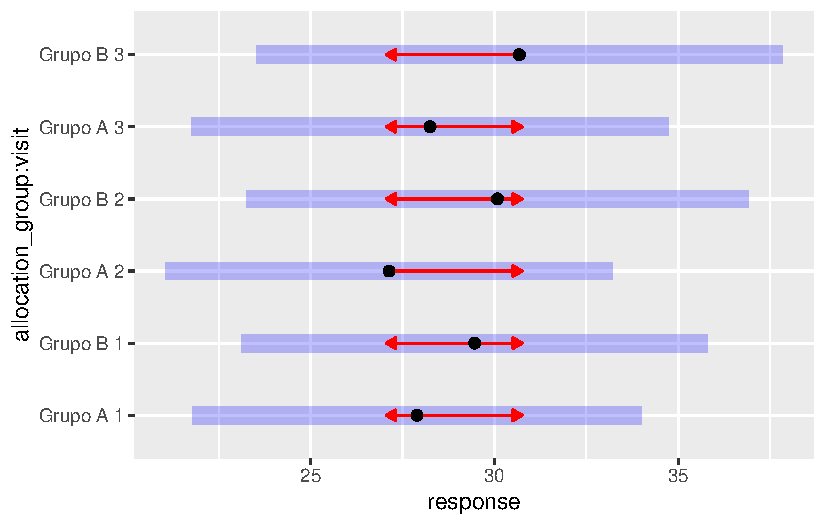
\includegraphics{Outcomes_V1V2V3_files/figure-pdf/labs_ggt_raw_emm-1.pdf}

\begin{Shaded}
\begin{Highlighting}[]
\CommentTok{\# Get EMMs for each group at each visit}
\NormalTok{labs\_ggt\_emm }\OtherTok{\textless{}{-}}\NormalTok{ emmeans}\SpecialCharTok{::}\FunctionTok{emmeans}\NormalTok{(}
\NormalTok{    labs\_ggt\_model\_sens, }
    \SpecialCharTok{\textasciitilde{}}\NormalTok{ allocation\_group }\SpecialCharTok{*}\NormalTok{ visit}
\NormalTok{)}

\NormalTok{labs\_ggt\_emm }\OtherTok{\textless{}{-}} \FunctionTok{regrid}\NormalTok{(labs\_ggt\_emm)}

\CommentTok{\# Table of marginal means}
\NormalTok{labs\_ggt\_emm}
\end{Highlighting}
\end{Shaded}

\begin{verbatim}
 allocation_group visit response   SE   df lower.CL upper.CL
 Grupo A          1         23.8 2.32 74.8     19.2     28.5
 Grupo B          1         27.7 2.61 74.8     22.5     32.9
 Grupo A          2         23.6 2.34 80.4     18.9     28.2
 Grupo B          2         29.2 2.90 90.1     23.4     34.9
 Grupo A          3         24.8 2.53 88.4     19.8     29.8
 Grupo B          3         29.4 2.99 97.8     23.4     35.3

Degrees-of-freedom method: inherited from kenward-roger when re-gridding 
Confidence level used: 0.95 
\end{verbatim}

\begin{Shaded}
\begin{Highlighting}[]
\CommentTok{\# Pairwise comparisons: Between groups at each visit}
\NormalTok{emmeans}\SpecialCharTok{::}\FunctionTok{contrast}\NormalTok{(labs\_ggt\_emm, }\AttributeTok{method =} \StringTok{"pairwise"}\NormalTok{, }\AttributeTok{by =} \StringTok{"visit"}\NormalTok{, }\AttributeTok{adjust =} \StringTok{"bonferroni"}\NormalTok{) }\SpecialCharTok{\%\textgreater{}\%} \FunctionTok{summary}\NormalTok{(}\AttributeTok{infer =} \FunctionTok{c}\NormalTok{(}\ConstantTok{TRUE}\NormalTok{, }\ConstantTok{TRUE}\NormalTok{))}
\end{Highlighting}
\end{Shaded}

\begin{verbatim}
visit = 1:
 contrast          estimate   SE   df lower.CL upper.CL t.ratio p.value
 Grupo A - Grupo B    -3.87 3.49 74.8    -10.8     3.08  -1.110  0.2705

visit = 2:
 contrast          estimate   SE   df lower.CL upper.CL t.ratio p.value
 Grupo A - Grupo B    -5.63 3.73 80.4    -13.0     1.79  -1.510  0.1351

visit = 3:
 contrast          estimate   SE   df lower.CL upper.CL t.ratio p.value
 Grupo A - Grupo B    -4.54 3.92 88.4    -12.3     3.25  -1.158  0.2501

Degrees-of-freedom method: inherited from kenward-roger when re-gridding 
Confidence level used: 0.95 
\end{verbatim}

\begin{Shaded}
\begin{Highlighting}[]
\CommentTok{\# Pairwise comparisons: Changes over time within each group}
\NormalTok{emmeans}\SpecialCharTok{::}\FunctionTok{contrast}\NormalTok{(labs\_ggt\_emm, }\AttributeTok{method =} \StringTok{"pairwise"}\NormalTok{, }\AttributeTok{by =} \StringTok{"allocation\_group"}\NormalTok{, }\AttributeTok{adjust =} \StringTok{"bonferroni"}\NormalTok{) }\SpecialCharTok{\%\textgreater{}\%} \FunctionTok{summary}\NormalTok{(}\AttributeTok{infer =} \FunctionTok{c}\NormalTok{(}\ConstantTok{TRUE}\NormalTok{, }\ConstantTok{TRUE}\NormalTok{))}
\end{Highlighting}
\end{Shaded}

\begin{verbatim}
allocation_group = Grupo A:
 contrast        estimate   SE   df lower.CL upper.CL t.ratio p.value
 visit1 - visit2    0.273 1.25 74.8    -2.80     3.34   0.218  1.0000
 visit1 - visit3   -0.986 1.42 74.8    -4.46     2.49  -0.694  1.0000
 visit2 - visit3   -1.259 1.42 80.4    -4.73     2.21  -0.888  1.0000

allocation_group = Grupo B:
 contrast        estimate   SE   df lower.CL upper.CL t.ratio p.value
 visit1 - visit2   -1.479 1.64 74.8    -5.51     2.55  -0.899  1.0000
 visit1 - visit3   -1.649 1.78 74.8    -6.02     2.72  -0.924  1.0000
 visit2 - visit3   -0.170 1.88 90.1    -4.74     4.40  -0.091  1.0000

Degrees-of-freedom method: inherited from kenward-roger when re-gridding 
Confidence level used: 0.95 
Conf-level adjustment: bonferroni method for 3 estimates 
P value adjustment: bonferroni method for 3 tests 
\end{verbatim}

\begin{Shaded}
\begin{Highlighting}[]
\CommentTok{\# Plot of marginal means}
\FunctionTok{plot}\NormalTok{(labs\_ggt\_emm)}
\end{Highlighting}
\end{Shaded}

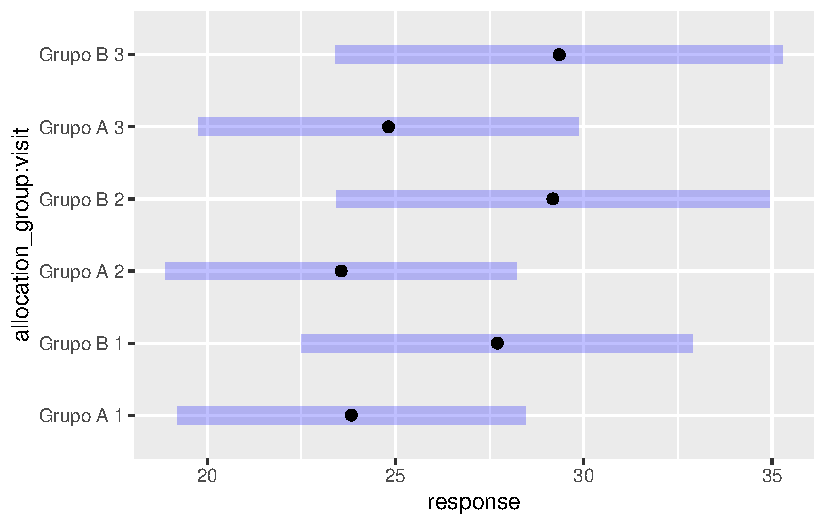
\includegraphics{Outcomes_V1V2V3_files/figure-pdf/labs_ggt_sens_emm-1.pdf}

\begin{Shaded}
\begin{Highlighting}[]
\FunctionTok{ggplot}\NormalTok{(}
    \AttributeTok{data =}\NormalTok{ data\_model, }
    \FunctionTok{aes}\NormalTok{(}
        \AttributeTok{x =} \FunctionTok{as.factor}\NormalTok{(visit),}
        \AttributeTok{y =}\NormalTok{ labs\_ggt,}
        \AttributeTok{group =}\NormalTok{ record\_id,}
\NormalTok{    )}
\NormalTok{) }\SpecialCharTok{+}
    \FunctionTok{geom\_line}\NormalTok{(}\AttributeTok{alpha =} \FloatTok{0.5}\NormalTok{) }\SpecialCharTok{+}
    \FunctionTok{geom\_point}\NormalTok{(}\AttributeTok{alpha =} \FloatTok{0.7}\NormalTok{) }\SpecialCharTok{+}
    \FunctionTok{geom\_smooth}\NormalTok{(}
        \FunctionTok{aes}\NormalTok{(}\AttributeTok{group =}\NormalTok{ allocation\_group),}
        \AttributeTok{method =} \StringTok{"lm"}\NormalTok{,}
        \AttributeTok{se =} \ConstantTok{TRUE}\NormalTok{,}
        \AttributeTok{linewidth =} \DecValTok{1}
\NormalTok{    ) }\SpecialCharTok{+}
    \FunctionTok{labs}\NormalTok{(}\AttributeTok{title =} \StringTok{"All data"}\NormalTok{) }\SpecialCharTok{+}
    \FunctionTok{facet\_wrap}\NormalTok{(}\SpecialCharTok{\textasciitilde{}}\NormalTok{ allocation\_group) }
\end{Highlighting}
\end{Shaded}

\begin{verbatim}
`geom_smooth()` using formula = 'y ~ x'
\end{verbatim}

\begin{verbatim}
Warning: Removed 11 rows containing non-finite outside the scale range
(`stat_smooth()`).
\end{verbatim}

\begin{verbatim}
Warning: Removed 9 rows containing missing values or values outside the scale range
(`geom_line()`).
\end{verbatim}

\begin{verbatim}
Warning: Removed 11 rows containing missing values or values outside the scale range
(`geom_point()`).
\end{verbatim}

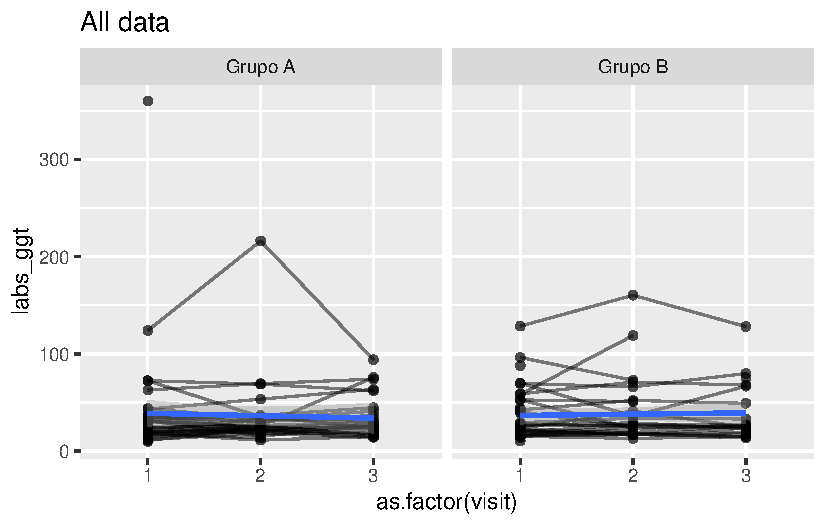
\includegraphics{Outcomes_V1V2V3_files/figure-pdf/labs_ggt_6-1.pdf}

\begin{Shaded}
\begin{Highlighting}[]
    \CommentTok{\#coord\_cartesian(ylim = c(10, 150))}

\NormalTok{data\_model }\SpecialCharTok{\%\textgreater{}\%} 
    \FunctionTok{filter}\NormalTok{(}
        \SpecialCharTok{!}\NormalTok{(record\_id }\SpecialCharTok{\%in\%}\NormalTok{ labs\_ggt\_model\_check}\SpecialCharTok{$}\NormalTok{influential\_ids)}
\NormalTok{    ) }\SpecialCharTok{\%\textgreater{}\%} 
    \FunctionTok{ggplot}\NormalTok{(}
        \FunctionTok{aes}\NormalTok{(}
            \AttributeTok{x =} \FunctionTok{as.factor}\NormalTok{(visit),}
            \AttributeTok{y =}\NormalTok{ labs\_ggt,}
            \AttributeTok{group =}\NormalTok{ record\_id,}
\NormalTok{        )}
\NormalTok{    ) }\SpecialCharTok{+}
    \FunctionTok{geom\_line}\NormalTok{(}\AttributeTok{alpha =} \FloatTok{0.5}\NormalTok{) }\SpecialCharTok{+}
    \FunctionTok{geom\_point}\NormalTok{(}\AttributeTok{alpha =} \FloatTok{0.7}\NormalTok{) }\SpecialCharTok{+}
    \FunctionTok{geom\_smooth}\NormalTok{(}
        \FunctionTok{aes}\NormalTok{(}\AttributeTok{group =}\NormalTok{ allocation\_group),}
        \AttributeTok{method =} \StringTok{"lm"}\NormalTok{,}
        \AttributeTok{se =} \ConstantTok{TRUE}\NormalTok{,}
        \AttributeTok{linewidth =} \DecValTok{1}
\NormalTok{    ) }\SpecialCharTok{+}
    \FunctionTok{labs}\NormalTok{(}\AttributeTok{title =} \StringTok{"Sensitivity analysis"}\NormalTok{) }\SpecialCharTok{+}
    \FunctionTok{facet\_wrap}\NormalTok{(}\SpecialCharTok{\textasciitilde{}}\NormalTok{ allocation\_group) }
\end{Highlighting}
\end{Shaded}

\begin{verbatim}
`geom_smooth()` using formula = 'y ~ x'
\end{verbatim}

\begin{verbatim}
Warning: Removed 10 rows containing non-finite outside the scale range
(`stat_smooth()`).
\end{verbatim}

\begin{verbatim}
Warning: Removed 8 rows containing missing values or values outside the scale range
(`geom_line()`).
\end{verbatim}

\begin{verbatim}
Warning: Removed 10 rows containing missing values or values outside the scale range
(`geom_point()`).
\end{verbatim}

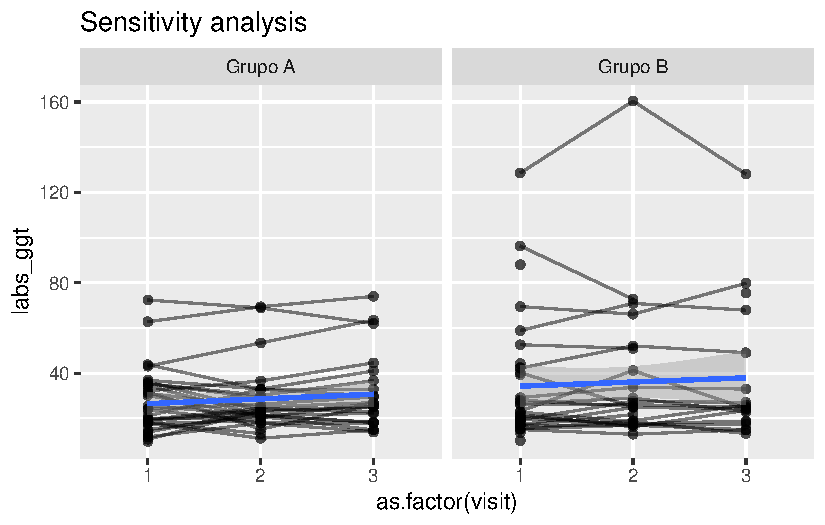
\includegraphics{Outcomes_V1V2V3_files/figure-pdf/labs_ggt_6-2.pdf}

\begin{Shaded}
\begin{Highlighting}[]
    \CommentTok{\#coord\_cartesian(ylim = c(10, 150))}
\end{Highlighting}
\end{Shaded}

\subsubsection{Fosfatase Alcalina}\label{fosfatase-alcalina}

Variável: \texttt{labs\_alkp}

\begin{Shaded}
\begin{Highlighting}[]
\CommentTok{\# Plot 1: Raw data}
\NormalTok{labs\_alkp\_hist\_1 }\OtherTok{\textless{}{-}}\NormalTok{ data\_model }\SpecialCharTok{\%\textgreater{}\%} 
    \CommentTok{\#filter(}
    \CommentTok{\#    labs\_alkp \textless{} 300}
    \CommentTok{\#) \%\textgreater{}\% }
    \FunctionTok{ggplot}\NormalTok{(}\FunctionTok{aes}\NormalTok{(}\AttributeTok{x =}\NormalTok{ labs\_alkp)) }\SpecialCharTok{+} 
    \FunctionTok{geom\_histogram}\NormalTok{(}\AttributeTok{bins =} \DecValTok{50}\NormalTok{, }\AttributeTok{fill =} \StringTok{"skyblue"}\NormalTok{, }\AttributeTok{color =} \StringTok{"black"}\NormalTok{)}

\CommentTok{\# Plot 2: Log{-}transformed data}
\NormalTok{labs\_alkp\_hist\_2 }\OtherTok{\textless{}{-}}\NormalTok{ data\_model }\SpecialCharTok{\%\textgreater{}\%} 
    \CommentTok{\#filter(}
    \CommentTok{\#    labs\_alkp \textless{} 300}
    \CommentTok{\#) \%\textgreater{}\%}
    \FunctionTok{ggplot}\NormalTok{(}\FunctionTok{aes}\NormalTok{(}\AttributeTok{x =} \FunctionTok{log1p}\NormalTok{(labs\_alkp))) }\SpecialCharTok{+} 
    \FunctionTok{geom\_histogram}\NormalTok{(}\AttributeTok{bins =} \DecValTok{50}\NormalTok{, }\AttributeTok{fill =} \StringTok{"lightgreen"}\NormalTok{, }\AttributeTok{color =} \StringTok{"black"}\NormalTok{)}

\CommentTok{\# Combine side by side}
\NormalTok{labs\_alkp\_hist\_1 }\SpecialCharTok{+}\NormalTok{ labs\_alkp\_hist\_2 }\CommentTok{\# library(patchwork)}
\end{Highlighting}
\end{Shaded}

\begin{verbatim}
Warning: Removed 11 rows containing non-finite outside the scale range (`stat_bin()`).
Removed 11 rows containing non-finite outside the scale range (`stat_bin()`).
\end{verbatim}

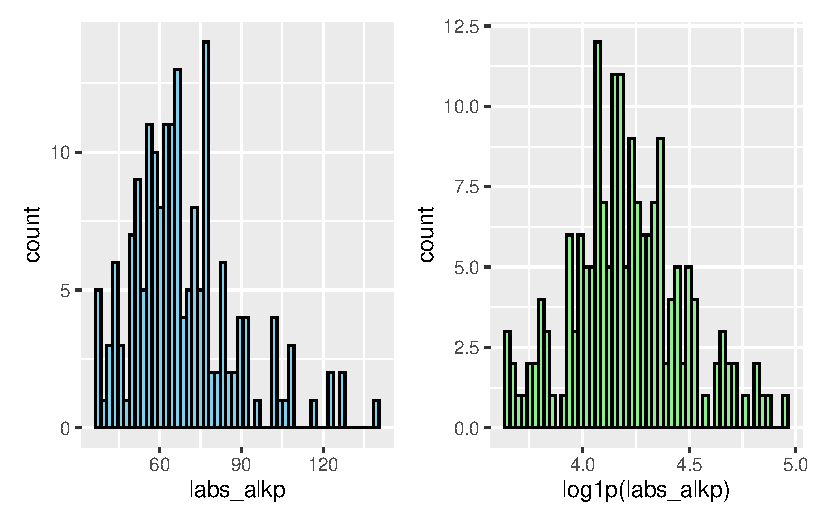
\includegraphics{Outcomes_V1V2V3_files/figure-pdf/labs_alkp_1-1.pdf}

\begin{Shaded}
\begin{Highlighting}[]
\CommentTok{\# LMM}
\NormalTok{labs\_alkp\_model }\OtherTok{\textless{}{-}} \FunctionTok{lmer}\NormalTok{(}\FunctionTok{log1p}\NormalTok{(labs\_alkp) }\SpecialCharTok{\textasciitilde{}}\NormalTok{ allocation\_group }\SpecialCharTok{*}\NormalTok{ visit }\SpecialCharTok{+}\NormalTok{ (}\DecValTok{1} \SpecialCharTok{|}\NormalTok{ record\_id), }\AttributeTok{data =}\NormalTok{ data\_model)}
\FunctionTok{check\_collinearity}\NormalTok{(labs\_alkp\_model)}
\end{Highlighting}
\end{Shaded}

\begin{verbatim}
# Check for Multicollinearity

Low Correlation

                   Term  VIF   VIF 95% CI Increased SE Tolerance
       allocation_group 1.08 [1.01, 1.62]         1.04      0.93
                  visit 3.40 [2.71, 4.36]         1.84      0.29
 allocation_group:visit 3.52 [2.80, 4.52]         1.88      0.28
 Tolerance 95% CI
     [0.62, 0.99]
     [0.23, 0.37]
     [0.22, 0.36]
\end{verbatim}

\begin{Shaded}
\begin{Highlighting}[]
\CommentTok{\# Sensitivity analysis}
\NormalTok{labs\_alkp\_model\_check }\OtherTok{\textless{}{-}} \FunctionTok{sensitivity\_check\_lmer}\NormalTok{(}
    \AttributeTok{model =}\NormalTok{ labs\_alkp\_model,}
    \AttributeTok{id\_var =} \StringTok{"record\_id"}\NormalTok{,}
    \AttributeTok{top\_n =} \DecValTok{4}\NormalTok{)}

\CommentTok{\# LMM Sensitivity}
\NormalTok{labs\_alkp\_model\_sens }\OtherTok{\textless{}{-}} \FunctionTok{update}\NormalTok{(}\AttributeTok{object =}\NormalTok{ labs\_alkp\_model,}
                              \AttributeTok{subset =} \SpecialCharTok{!}\NormalTok{(record\_id }\SpecialCharTok{\%in\%}\NormalTok{ labs\_alkp\_model\_check}\SpecialCharTok{$}\NormalTok{influential\_ids))}
\CommentTok{\# Influential IDS}
\NormalTok{labs\_alkp\_model\_check}\SpecialCharTok{$}\NormalTok{influential\_ids}
\end{Highlighting}
\end{Shaded}

\begin{verbatim}
[1] "56" "75" "53" "3" 
\end{verbatim}

\paragraph{Resumo dos modelos}\label{resumo-dos-modelos-3}

\begin{Shaded}
\begin{Highlighting}[]
\CommentTok{\# Model comparison}
\FunctionTok{summary}\NormalTok{(labs\_alkp\_model)}
\end{Highlighting}
\end{Shaded}

\begin{verbatim}
Linear mixed model fit by REML. t-tests use Satterthwaite's method [
lmerModLmerTest]
Formula: log1p(labs_alkp) ~ allocation_group * visit + (1 | record_id)
   Data: data_model

REML criterion at convergence: -87.9

Scaled residuals: 
     Min       1Q   Median       3Q      Max 
-2.02732 -0.46612  0.01043  0.43200  2.62132 

Random effects:
 Groups    Name        Variance Std.Dev.
 record_id (Intercept) 0.06041  0.2458  
 Residual              0.01021  0.1010  
Number of obs: 178, groups:  record_id, 75

Fixed effects:
                                 Estimate Std. Error         df t value
(Intercept)                      4.210088   0.043688  84.150015  96.367
allocation_groupGrupo B          0.033160   0.061377  84.150015   0.540
visit2                          -0.046856   0.025510 100.999520  -1.837
visit3                          -0.030253   0.027680 101.476417  -1.093
allocation_groupGrupo B:visit2   0.018421   0.037511 101.816342   0.491
allocation_groupGrupo B:visit3   0.004182   0.040741 102.191761   0.103
                               Pr(>|t|)    
(Intercept)                      <2e-16 ***
allocation_groupGrupo B          0.5904    
visit2                           0.0692 .  
visit3                           0.2770    
allocation_groupGrupo B:visit2   0.6244    
allocation_groupGrupo B:visit3   0.9184    
---
Signif. codes:  0 '***' 0.001 '**' 0.01 '*' 0.05 '.' 0.1 ' ' 1

Correlation of Fixed Effects:
            (Intr) all_GB visit2 visit3 a_GB:2
allctn_grGB -0.712                            
visit2      -0.248  0.176                     
visit3      -0.228  0.162  0.455              
allctn_GB:2  0.168 -0.236 -0.680 -0.310       
allctn_GB:3  0.155 -0.218 -0.309 -0.679  0.436
\end{verbatim}

\begin{Shaded}
\begin{Highlighting}[]
\FunctionTok{summary}\NormalTok{(labs\_alkp\_model\_sens)}
\end{Highlighting}
\end{Shaded}

\begin{verbatim}
Linear mixed model fit by REML. t-tests use Satterthwaite's method [
lmerModLmerTest]
Formula: log1p(labs_alkp) ~ allocation_group * visit + (1 | record_id)
   Data: data_model
 Subset: !(record_id %in% labs_alkp_model_check$influential_ids)

REML criterion at convergence: -118.6

Scaled residuals: 
     Min       1Q   Median       3Q      Max 
-1.95508 -0.49130  0.04228  0.50567  1.80928 

Random effects:
 Groups    Name        Variance Std.Dev.
 record_id (Intercept) 0.06287  0.25073 
 Residual              0.00669  0.08179 
Number of obs: 167, groups:  record_id, 71

Fixed effects:
                                Estimate Std. Error        df t value Pr(>|t|)
(Intercept)                     4.198426   0.044579 75.550975  94.179   <2e-16
allocation_groupGrupo B         0.071738   0.062605 75.550975   1.146    0.255
visit2                         -0.021391   0.021391 93.237481  -1.000    0.320
visit3                         -0.002867   0.023373 93.517548  -0.123    0.903
allocation_groupGrupo B:visit2 -0.020052   0.031577 93.770609  -0.635    0.527
allocation_groupGrupo B:visit3 -0.052680   0.034183 93.954152  -1.541    0.127
                                  
(Intercept)                    ***
allocation_groupGrupo B           
visit2                            
visit3                            
allocation_groupGrupo B:visit2    
allocation_groupGrupo B:visit3    
---
Signif. codes:  0 '***' 0.001 '**' 0.01 '*' 0.05 '.' 0.1 ' ' 1

Correlation of Fixed Effects:
            (Intr) all_GB visit2 visit3 a_GB:2
allctn_grGB -0.712                            
visit2      -0.200  0.143                     
visit3      -0.183  0.131  0.454              
allctn_GB:2  0.136 -0.191 -0.677 -0.307       
allctn_GB:3  0.125 -0.176 -0.310 -0.684  0.438
\end{verbatim}

\begin{Shaded}
\begin{Highlighting}[]
\NormalTok{labs\_alkp\_model\_check}\SpecialCharTok{$}\NormalTok{comparison\_table}
\end{Highlighting}
\end{Shaded}

\begin{verbatim}
# A tibble: 16 x 6
   Model       term                       estimate std.error statistic   p.value
   <chr>       <chr>                         <dbl>     <dbl>     <dbl>     <dbl>
 1 Original    (Intercept)                 4.21       0.0437    96.4    6.67e-88
 2 Sensitivity (Intercept)                 4.20       0.0446    94.2    4.38e-80
 3 Original    allocation_groupGrupo B     0.0332     0.0614     0.540  5.90e- 1
 4 Sensitivity allocation_groupGrupo B     0.0717     0.0626     1.15   2.55e- 1
 5 Original    allocation_groupGrupo B:v~  0.0184     0.0375     0.491  6.24e- 1
 6 Sensitivity allocation_groupGrupo B:v~ -0.0201     0.0316    -0.635  5.27e- 1
 7 Original    allocation_groupGrupo B:v~  0.00418    0.0407     0.103  9.18e- 1
 8 Sensitivity allocation_groupGrupo B:v~ -0.0527     0.0342    -1.54   1.27e- 1
 9 Original    sd__(Intercept)             0.246     NA         NA     NA       
10 Sensitivity sd__(Intercept)             0.251     NA         NA     NA       
11 Original    sd__Observation             0.101     NA         NA     NA       
12 Sensitivity sd__Observation             0.0818    NA         NA     NA       
13 Original    visit2                     -0.0469     0.0255    -1.84   6.92e- 2
14 Sensitivity visit2                     -0.0214     0.0214    -1.00   3.20e- 1
15 Original    visit3                     -0.0303     0.0277    -1.09   2.77e- 1
16 Sensitivity visit3                     -0.00287    0.0234    -0.123  9.03e- 1
\end{verbatim}

\begin{Shaded}
\begin{Highlighting}[]
\NormalTok{performance}\SpecialCharTok{::}\FunctionTok{compare\_performance}\NormalTok{(labs\_alkp\_model, labs\_alkp\_model\_sens)}
\end{Highlighting}
\end{Shaded}

\begin{verbatim}
When comparing models, please note that probably not all models were fit
  from same data.
\end{verbatim}

\begin{verbatim}
# Comparison of Model Performance Indices

Name                 |           Model |  AIC (weights) | AICc (weights)
------------------------------------------------------------------------
labs_alkp_model      | lmerModLmerTest | 1394.9 (<.001) | 1395.7 (<.001)
labs_alkp_model_sens | lmerModLmerTest | 1274.2 (>.999) | 1275.1 (>.999)

Name                 |  BIC (weights) | R2 (cond.) | R2 (marg.) |   ICC |  RMSE | Sigma
---------------------------------------------------------------------------------------
labs_alkp_model      | 1420.3 (<.001) |      0.857 |      0.010 | 0.855 | 0.077 | 0.101
labs_alkp_model_sens | 1299.1 (>.999) |      0.905 |      0.015 | 0.904 | 0.062 | 0.082
\end{verbatim}

\begin{Shaded}
\begin{Highlighting}[]
\NormalTok{performance}\SpecialCharTok{::}\FunctionTok{check\_model}\NormalTok{(labs\_alkp\_model)}
\end{Highlighting}
\end{Shaded}

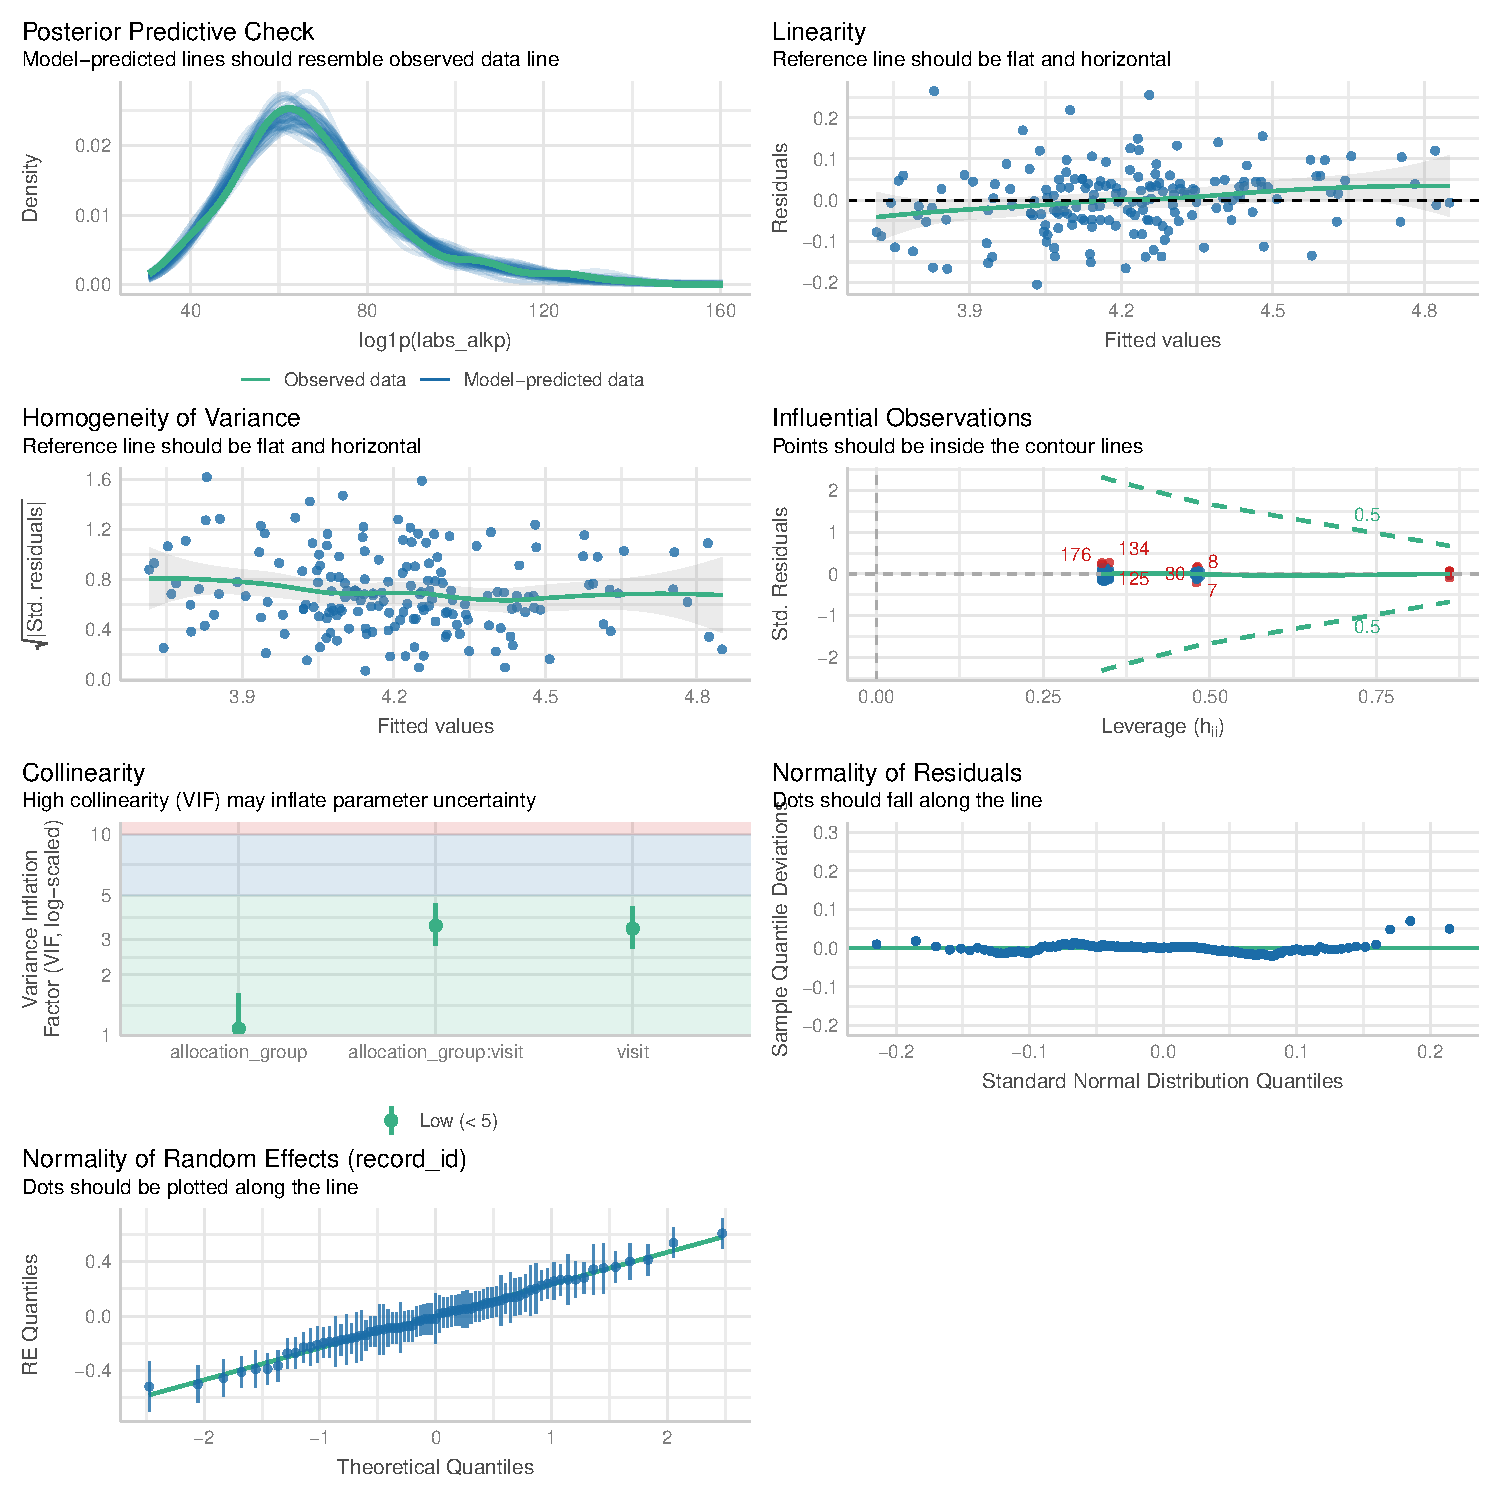
\includegraphics{Outcomes_V1V2V3_files/figure-pdf/labs_alkp_4-1.pdf}

\begin{Shaded}
\begin{Highlighting}[]
\NormalTok{performance}\SpecialCharTok{::}\FunctionTok{check\_model}\NormalTok{(labs\_alkp\_model\_sens)}
\end{Highlighting}
\end{Shaded}

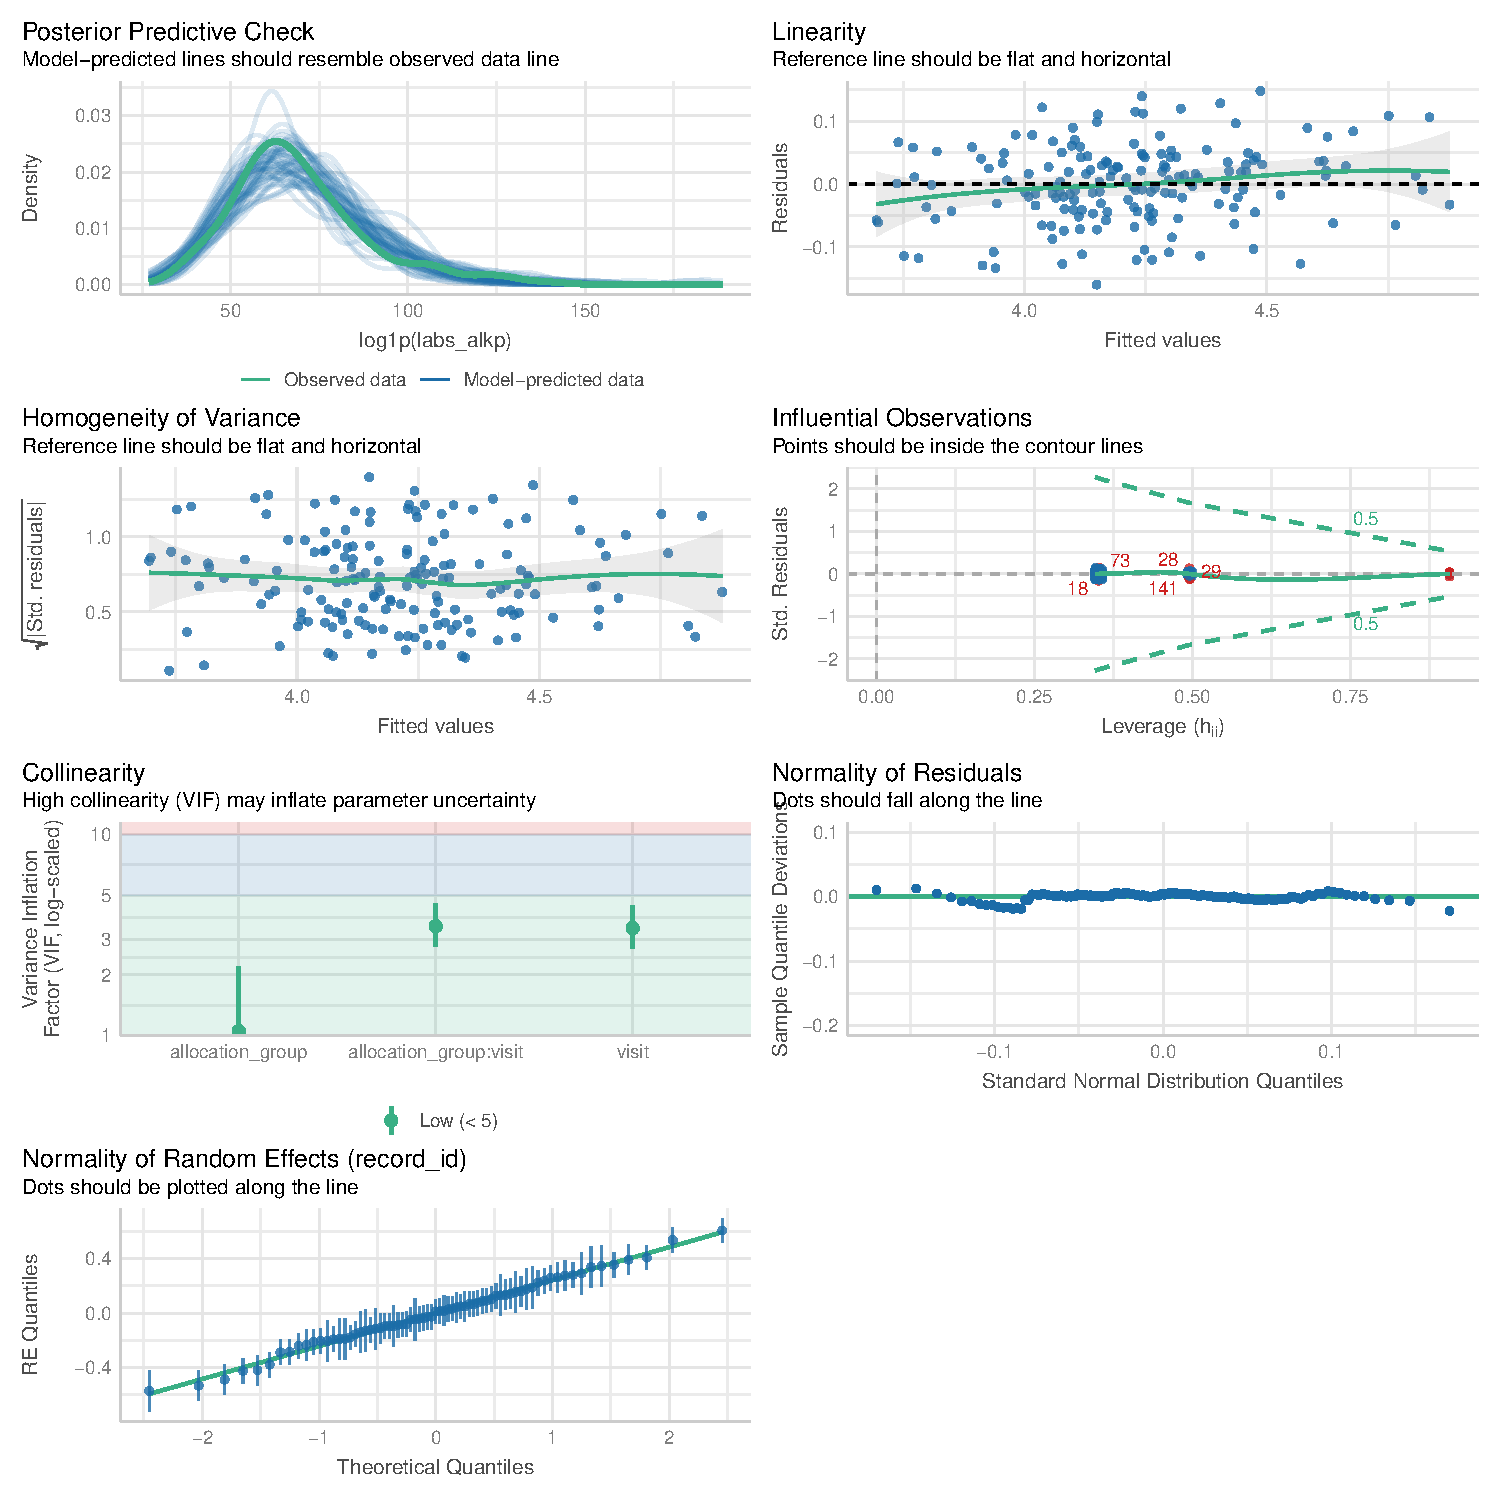
\includegraphics{Outcomes_V1V2V3_files/figure-pdf/labs_alkp_4-2.pdf}

\paragraph{Médias Marginais
Estimadas}\label{muxe9dias-marginais-estimadas-3}

\begin{Shaded}
\begin{Highlighting}[]
\CommentTok{\# Get EMMs for each group at each visit}
\NormalTok{labs\_alkp\_raw\_emm }\OtherTok{\textless{}{-}}\NormalTok{ emmeans}\SpecialCharTok{::}\FunctionTok{emmeans}\NormalTok{(}
\NormalTok{    labs\_alkp\_model, }
    \SpecialCharTok{\textasciitilde{}}\NormalTok{ allocation\_group }\SpecialCharTok{*}\NormalTok{ visit}
\NormalTok{)}

\NormalTok{labs\_alkp\_raw\_emm }\OtherTok{\textless{}{-}} \FunctionTok{regrid}\NormalTok{(labs\_alkp\_raw\_emm)}

\CommentTok{\# Table of marginal means}
\NormalTok{labs\_alkp\_raw\_emm}
\end{Highlighting}
\end{Shaded}

\begin{verbatim}
 allocation_group visit response   SE    df lower.CL upper.CL
 Grupo A          1         66.4 2.94  84.5     60.5     72.2
 Grupo B          1         68.6 3.00  84.5     62.7     74.6
 Grupo A          2         63.3 2.88  92.0     57.6     69.0
 Grupo B          2         66.7 3.09 101.5     60.6     72.8
 Grupo A          3         64.4 3.01 101.0     58.4     70.3
 Grupo B          3         66.8 3.19 112.0     60.5     73.2

Degrees-of-freedom method: inherited from kenward-roger when re-gridding 
Confidence level used: 0.95 
\end{verbatim}

\begin{Shaded}
\begin{Highlighting}[]
\CommentTok{\# Pairwise comparisons: Between groups at each visit}
\NormalTok{emmeans}\SpecialCharTok{::}\FunctionTok{contrast}\NormalTok{(labs\_alkp\_raw\_emm, }\AttributeTok{method =} \StringTok{"pairwise"}\NormalTok{, }\AttributeTok{by =} \StringTok{"visit"}\NormalTok{, }\AttributeTok{adjust =} \StringTok{"bonferroni"}\NormalTok{) }\SpecialCharTok{\%\textgreater{}\%} \FunctionTok{summary}\NormalTok{(}\AttributeTok{infer =} \FunctionTok{c}\NormalTok{(}\ConstantTok{TRUE}\NormalTok{, }\ConstantTok{TRUE}\NormalTok{))}
\end{Highlighting}
\end{Shaded}

\begin{verbatim}
visit = 1:
 contrast          estimate   SE    df lower.CL upper.CL t.ratio p.value
 Grupo A - Grupo B    -2.27 4.20  84.5    -10.6     6.09  -0.540  0.5904

visit = 2:
 contrast          estimate   SE    df lower.CL upper.CL t.ratio p.value
 Grupo A - Grupo B    -3.40 4.22  92.0    -11.8     4.98  -0.806  0.4223

visit = 3:
 contrast          estimate   SE    df lower.CL upper.CL t.ratio p.value
 Grupo A - Grupo B    -2.49 4.39 101.0    -11.2     6.22  -0.566  0.5724

Degrees-of-freedom method: inherited from kenward-roger when re-gridding 
Confidence level used: 0.95 
\end{verbatim}

\begin{Shaded}
\begin{Highlighting}[]
\CommentTok{\# Pairwise comparisons: Changes over time within each group}
\NormalTok{emmeans}\SpecialCharTok{::}\FunctionTok{contrast}\NormalTok{(labs\_alkp\_raw\_emm, }\AttributeTok{method =} \StringTok{"pairwise"}\NormalTok{, }\AttributeTok{by =} \StringTok{"allocation\_group"}\NormalTok{, }\AttributeTok{adjust =} \StringTok{"bonferroni"}\NormalTok{) }\SpecialCharTok{\%\textgreater{}\%} \FunctionTok{summary}\NormalTok{(}\AttributeTok{infer =} \FunctionTok{c}\NormalTok{(}\ConstantTok{TRUE}\NormalTok{, }\ConstantTok{TRUE}\NormalTok{))}
\end{Highlighting}
\end{Shaded}

\begin{verbatim}
allocation_group = Grupo A:
 contrast        estimate   SE    df lower.CL upper.CL t.ratio p.value
 visit1 - visit2     3.08 1.68  84.5    -1.02     7.18   1.837  0.2094
 visit1 - visit3     2.01 1.83  84.5    -2.47     6.48   1.096  0.8290
 visit2 - visit3    -1.08 1.81  92.0    -5.48     3.33  -0.596  1.0000

allocation_group = Grupo B:
 contrast        estimate   SE    df lower.CL upper.CL t.ratio p.value
 visit1 - visit2     1.95 1.88  84.5    -2.65     6.55   1.036  0.9090
 visit1 - visit3     1.79 2.05  84.5    -3.21     6.79   0.875  1.0000
 visit2 - visit3    -0.16 2.10 101.5    -5.28     4.96  -0.076  1.0000

Degrees-of-freedom method: inherited from kenward-roger when re-gridding 
Confidence level used: 0.95 
Conf-level adjustment: bonferroni method for 3 estimates 
P value adjustment: bonferroni method for 3 tests 
\end{verbatim}

\begin{Shaded}
\begin{Highlighting}[]
\CommentTok{\# Plot of marginal means}
\FunctionTok{plot}\NormalTok{(labs\_alkp\_raw\_emm)}
\end{Highlighting}
\end{Shaded}

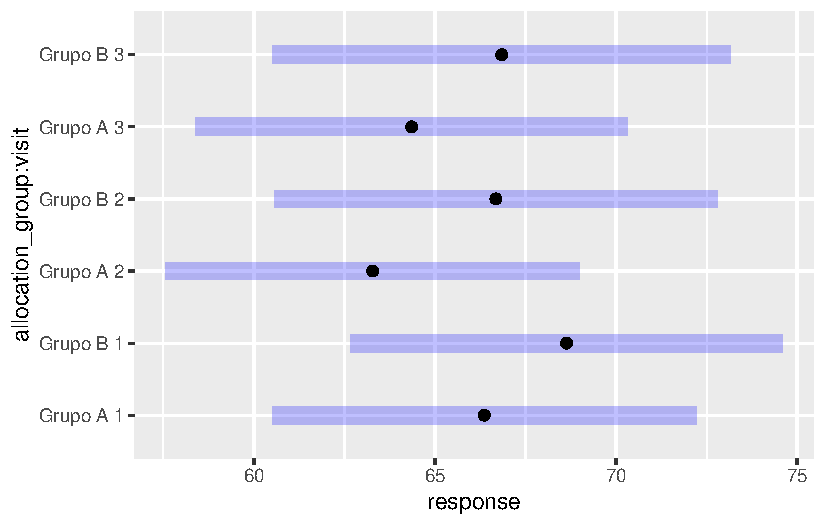
\includegraphics{Outcomes_V1V2V3_files/figure-pdf/labs_alkp_raw_emm-1.pdf}

\begin{Shaded}
\begin{Highlighting}[]
\CommentTok{\# Get EMMs for each group at each visit}
\NormalTok{labs\_alkp\_emm }\OtherTok{\textless{}{-}}\NormalTok{ emmeans}\SpecialCharTok{::}\FunctionTok{emmeans}\NormalTok{(}
\NormalTok{    labs\_alkp\_model\_sens, }
    \SpecialCharTok{\textasciitilde{}}\NormalTok{ allocation\_group }\SpecialCharTok{*}\NormalTok{ visit}
\NormalTok{)}

\CommentTok{\# Table of marginal means}
\NormalTok{labs\_alkp\_emm}
\end{Highlighting}
\end{Shaded}

\begin{verbatim}
 allocation_group visit emmean     SE   df lower.CL upper.CL
 Grupo A          1       4.20 0.0446 75.8     4.11     4.29
 Grupo B          1       4.27 0.0440 75.8     4.18     4.36
 Grupo A          2       4.18 0.0454 81.1     4.09     4.27
 Grupo B          2       4.23 0.0458 87.8     4.14     4.32
 Grupo A          3       4.20 0.0464 87.4     4.10     4.29
 Grupo B          3       4.21 0.0467 93.8     4.12     4.31

Degrees-of-freedom method: kenward-roger 
Results are given on the log1p (not the response) scale. 
Confidence level used: 0.95 
\end{verbatim}

\begin{Shaded}
\begin{Highlighting}[]
\CommentTok{\# Pairwise comparisons: Between groups at each visit}
\NormalTok{emmeans}\SpecialCharTok{::}\FunctionTok{contrast}\NormalTok{(labs\_alkp\_emm, }\AttributeTok{method =} \StringTok{"pairwise"}\NormalTok{, }\AttributeTok{by =} \StringTok{"visit"}\NormalTok{, }\AttributeTok{adjust =} \StringTok{"bonferroni"}\NormalTok{) }\SpecialCharTok{\%\textgreater{}\%} \FunctionTok{summary}\NormalTok{(}\AttributeTok{infer =} \FunctionTok{c}\NormalTok{(}\ConstantTok{TRUE}\NormalTok{, }\ConstantTok{TRUE}\NormalTok{))}
\end{Highlighting}
\end{Shaded}

\begin{verbatim}
visit = 1:
 contrast          estimate     SE   df lower.CL upper.CL t.ratio p.value
 Grupo A - Grupo B  -0.0717 0.0626 75.8   -0.196   0.0530  -1.146  0.2554

visit = 2:
 contrast          estimate     SE   df lower.CL upper.CL t.ratio p.value
 Grupo A - Grupo B  -0.0517 0.0645 84.4   -0.180   0.0766  -0.801  0.4254

visit = 3:
 contrast          estimate     SE   df lower.CL upper.CL t.ratio p.value
 Grupo A - Grupo B  -0.0191 0.0658 90.6   -0.150   0.1117  -0.289  0.7729

Note: contrasts are still on the log1p scale. Consider using
      regrid() if you want contrasts of back-transformed estimates. 
Degrees-of-freedom method: kenward-roger 
Confidence level used: 0.95 
\end{verbatim}

\begin{Shaded}
\begin{Highlighting}[]
\CommentTok{\# Pairwise comparisons: Changes over time within each group}
\NormalTok{emmeans}\SpecialCharTok{::}\FunctionTok{contrast}\NormalTok{(labs\_alkp\_emm, }\AttributeTok{method =} \StringTok{"pairwise"}\NormalTok{, }\AttributeTok{by =} \StringTok{"allocation\_group"}\NormalTok{, }\AttributeTok{adjust =} \StringTok{"bonferroni"}\NormalTok{) }\SpecialCharTok{\%\textgreater{}\%} \FunctionTok{summary}\NormalTok{(}\AttributeTok{infer =} \FunctionTok{c}\NormalTok{(}\ConstantTok{TRUE}\NormalTok{, }\ConstantTok{TRUE}\NormalTok{))}
\end{Highlighting}
\end{Shaded}

\begin{verbatim}
allocation_group = Grupo A:
 contrast        estimate     SE   df lower.CL upper.CL t.ratio p.value
 visit1 - visit2  0.02139 0.0214 93.5 -0.03077   0.0736   1.000  0.9602
 visit1 - visit3  0.00287 0.0234 93.8 -0.05413   0.0599   0.123  1.0000
 visit2 - visit3 -0.01852 0.0235 92.6 -0.07572   0.0387  -0.790  1.0000

allocation_group = Grupo B:
 contrast        estimate     SE   df lower.CL upper.CL t.ratio p.value
 visit1 - visit2  0.04144 0.0232 94.5 -0.01521   0.0981   1.783  0.2333
 visit1 - visit3  0.05555 0.0250 94.6 -0.00529   0.1164   2.225  0.0853
 visit2 - visit3  0.01410 0.0259 92.9 -0.04902   0.0772   0.545  1.0000

Note: contrasts are still on the log1p scale. Consider using
      regrid() if you want contrasts of back-transformed estimates. 
Degrees-of-freedom method: kenward-roger 
Confidence level used: 0.95 
Conf-level adjustment: bonferroni method for 3 estimates 
P value adjustment: bonferroni method for 3 tests 
\end{verbatim}

\begin{Shaded}
\begin{Highlighting}[]
\CommentTok{\# Plot of marginal means}
\FunctionTok{plot}\NormalTok{(labs\_alkp\_emm)}
\end{Highlighting}
\end{Shaded}

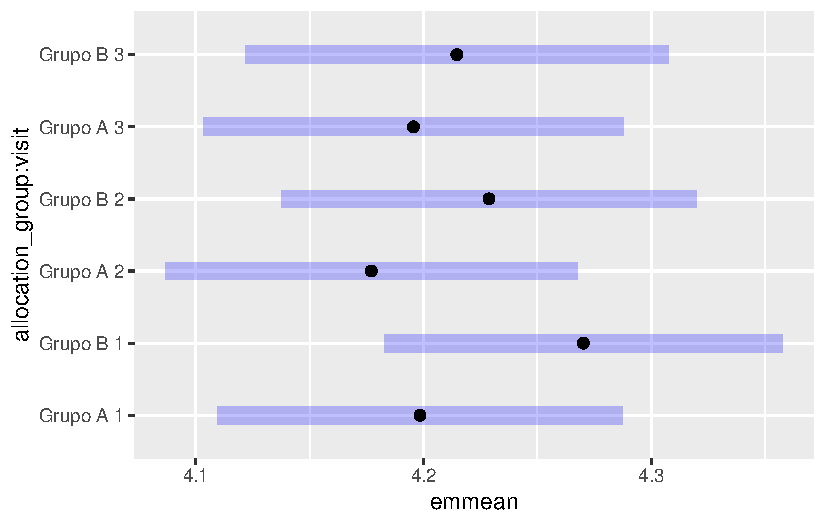
\includegraphics{Outcomes_V1V2V3_files/figure-pdf/labs_alkp_sens_emm-1.pdf}

\begin{Shaded}
\begin{Highlighting}[]
\FunctionTok{ggplot}\NormalTok{(}
    \AttributeTok{data =}\NormalTok{ data\_model, }
    \FunctionTok{aes}\NormalTok{(}
        \AttributeTok{x =} \FunctionTok{as.factor}\NormalTok{(visit),}
        \AttributeTok{y =}\NormalTok{ labs\_alkp,}
        \AttributeTok{group =}\NormalTok{ record\_id,}
\NormalTok{    )}
\NormalTok{) }\SpecialCharTok{+}
    \FunctionTok{geom\_line}\NormalTok{(}\AttributeTok{alpha =} \FloatTok{0.5}\NormalTok{) }\SpecialCharTok{+}
    \FunctionTok{geom\_point}\NormalTok{(}\AttributeTok{alpha =} \FloatTok{0.7}\NormalTok{) }\SpecialCharTok{+}
    \FunctionTok{geom\_smooth}\NormalTok{(}
        \FunctionTok{aes}\NormalTok{(}\AttributeTok{group =}\NormalTok{ allocation\_group),}
        \AttributeTok{method =} \StringTok{"lm"}\NormalTok{,}
        \AttributeTok{se =} \ConstantTok{TRUE}\NormalTok{,}
        \AttributeTok{linewidth =} \DecValTok{1}
\NormalTok{    ) }\SpecialCharTok{+}
    \FunctionTok{labs}\NormalTok{(}\AttributeTok{title =} \StringTok{"All data"}\NormalTok{) }\SpecialCharTok{+}
    \FunctionTok{facet\_wrap}\NormalTok{(}\SpecialCharTok{\textasciitilde{}}\NormalTok{ allocation\_group) }
\end{Highlighting}
\end{Shaded}

\begin{verbatim}
`geom_smooth()` using formula = 'y ~ x'
\end{verbatim}

\begin{verbatim}
Warning: Removed 11 rows containing non-finite outside the scale range
(`stat_smooth()`).
\end{verbatim}

\begin{verbatim}
Warning: Removed 9 rows containing missing values or values outside the scale range
(`geom_line()`).
\end{verbatim}

\begin{verbatim}
Warning: Removed 11 rows containing missing values or values outside the scale range
(`geom_point()`).
\end{verbatim}

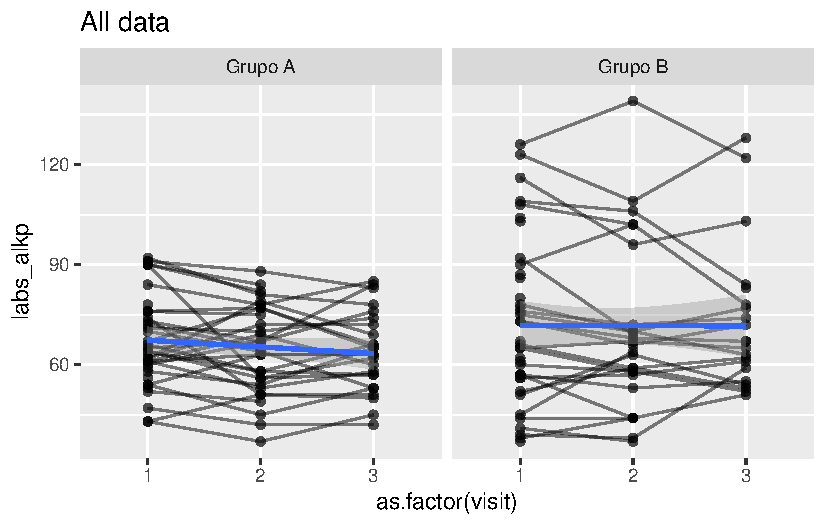
\includegraphics{Outcomes_V1V2V3_files/figure-pdf/labs_alkp_6-1.pdf}

\begin{Shaded}
\begin{Highlighting}[]
    \CommentTok{\#coord\_cartesian(ylim = c(10, 150))}

\NormalTok{data\_model }\SpecialCharTok{\%\textgreater{}\%} 
    \FunctionTok{filter}\NormalTok{(}
        \SpecialCharTok{!}\NormalTok{(record\_id }\SpecialCharTok{\%in\%}\NormalTok{ labs\_alkp\_model\_check}\SpecialCharTok{$}\NormalTok{influential\_ids)}
\NormalTok{    ) }\SpecialCharTok{\%\textgreater{}\%} 
    \FunctionTok{ggplot}\NormalTok{(}
        \FunctionTok{aes}\NormalTok{(}
            \AttributeTok{x =} \FunctionTok{as.factor}\NormalTok{(visit),}
            \AttributeTok{y =}\NormalTok{ labs\_alkp,}
            \AttributeTok{group =}\NormalTok{ record\_id,}
\NormalTok{        )}
\NormalTok{    ) }\SpecialCharTok{+}
    \FunctionTok{geom\_line}\NormalTok{(}\AttributeTok{alpha =} \FloatTok{0.5}\NormalTok{) }\SpecialCharTok{+}
    \FunctionTok{geom\_point}\NormalTok{(}\AttributeTok{alpha =} \FloatTok{0.7}\NormalTok{) }\SpecialCharTok{+}
    \FunctionTok{geom\_smooth}\NormalTok{(}
        \FunctionTok{aes}\NormalTok{(}\AttributeTok{group =}\NormalTok{ allocation\_group),}
        \AttributeTok{method =} \StringTok{"lm"}\NormalTok{,}
        \AttributeTok{se =} \ConstantTok{TRUE}\NormalTok{,}
        \AttributeTok{linewidth =} \DecValTok{1}
\NormalTok{    ) }\SpecialCharTok{+}
    \FunctionTok{labs}\NormalTok{(}\AttributeTok{title =} \StringTok{"Sensitivity analysis"}\NormalTok{) }\SpecialCharTok{+}
    \FunctionTok{facet\_wrap}\NormalTok{(}\SpecialCharTok{\textasciitilde{}}\NormalTok{ allocation\_group) }
\end{Highlighting}
\end{Shaded}

\begin{verbatim}
`geom_smooth()` using formula = 'y ~ x'
\end{verbatim}

\begin{verbatim}
Warning: Removed 11 rows containing non-finite outside the scale range
(`stat_smooth()`).
\end{verbatim}

\begin{verbatim}
Warning: Removed 9 rows containing missing values or values outside the scale range
(`geom_line()`).
\end{verbatim}

\begin{verbatim}
Warning: Removed 11 rows containing missing values or values outside the scale range
(`geom_point()`).
\end{verbatim}

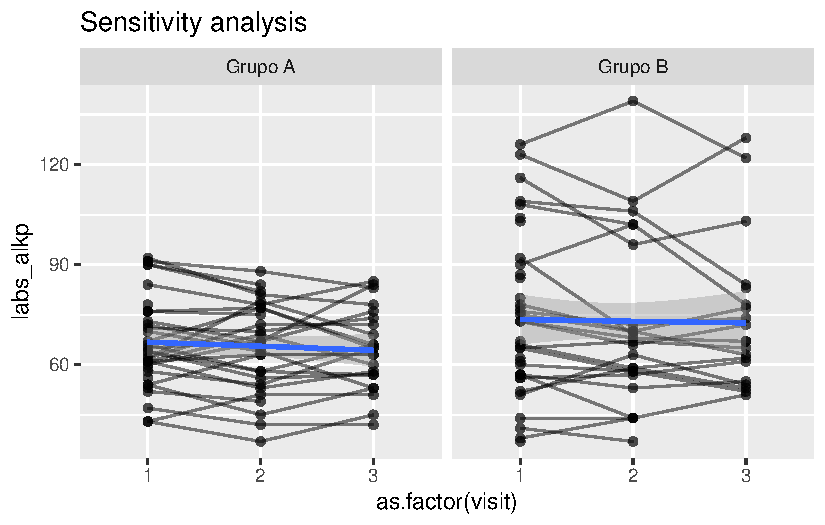
\includegraphics{Outcomes_V1V2V3_files/figure-pdf/labs_alkp_6-2.pdf}

\begin{Shaded}
\begin{Highlighting}[]
    \CommentTok{\#coord\_cartesian(ylim = c(10, 150))}
\end{Highlighting}
\end{Shaded}

\subsubsection{Colesterol Total}\label{colesterol-total}

Variável: \texttt{labs\_cholesterol}

\begin{Shaded}
\begin{Highlighting}[]
\CommentTok{\# Plot 1: Raw data}
\NormalTok{labs\_cholesterol\_hist\_1 }\OtherTok{\textless{}{-}}\NormalTok{ data\_model }\SpecialCharTok{\%\textgreater{}\%} 
    \CommentTok{\#filter(}
    \CommentTok{\#    labs\_cholesterol \textless{} 300}
    \CommentTok{\#) \%\textgreater{}\% }
    \FunctionTok{ggplot}\NormalTok{(}\FunctionTok{aes}\NormalTok{(}\AttributeTok{x =}\NormalTok{ labs\_cholesterol)) }\SpecialCharTok{+} 
    \FunctionTok{geom\_histogram}\NormalTok{(}\AttributeTok{bins =} \DecValTok{50}\NormalTok{, }\AttributeTok{fill =} \StringTok{"skyblue"}\NormalTok{, }\AttributeTok{color =} \StringTok{"black"}\NormalTok{)}

\CommentTok{\# Plot 2: Log{-}transformed data}
\NormalTok{labs\_cholesterol\_hist\_2 }\OtherTok{\textless{}{-}}\NormalTok{ data\_model }\SpecialCharTok{\%\textgreater{}\%} 
    \CommentTok{\#filter(}
    \CommentTok{\#    labs\_cholesterol \textless{} 300}
    \CommentTok{\#) \%\textgreater{}\%}
    \FunctionTok{ggplot}\NormalTok{(}\FunctionTok{aes}\NormalTok{(}\AttributeTok{x =} \FunctionTok{log1p}\NormalTok{(labs\_cholesterol))) }\SpecialCharTok{+} 
    \FunctionTok{geom\_histogram}\NormalTok{(}\AttributeTok{bins =} \DecValTok{50}\NormalTok{, }\AttributeTok{fill =} \StringTok{"lightgreen"}\NormalTok{, }\AttributeTok{color =} \StringTok{"black"}\NormalTok{)}

\CommentTok{\# Combine side by side}
\NormalTok{labs\_cholesterol\_hist\_1 }\SpecialCharTok{+}\NormalTok{ labs\_cholesterol\_hist\_2 }\CommentTok{\# library(patchwork)}
\end{Highlighting}
\end{Shaded}

\begin{verbatim}
Warning: Removed 10 rows containing non-finite outside the scale range (`stat_bin()`).
Removed 10 rows containing non-finite outside the scale range (`stat_bin()`).
\end{verbatim}

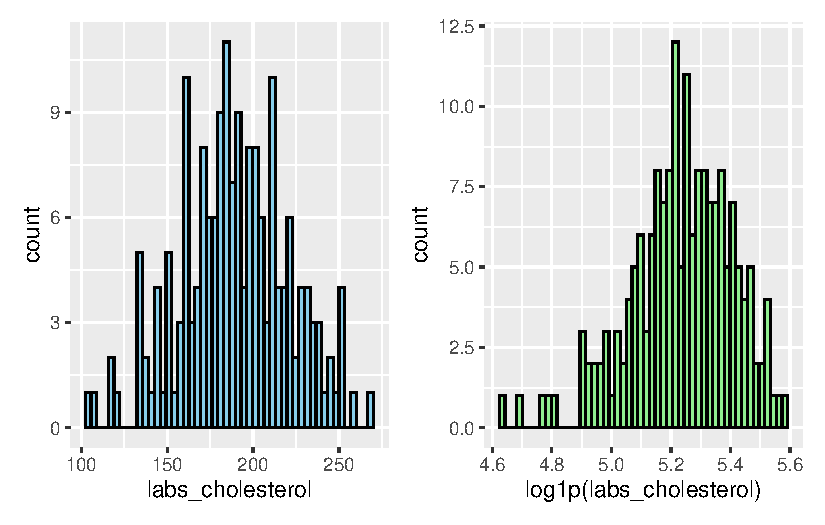
\includegraphics{Outcomes_V1V2V3_files/figure-pdf/labs_cholesterol_1-1.pdf}

\begin{Shaded}
\begin{Highlighting}[]
\CommentTok{\# LMM}
\NormalTok{labs\_cholesterol\_model }\OtherTok{\textless{}{-}} \FunctionTok{lmer}\NormalTok{(labs\_cholesterol }\SpecialCharTok{\textasciitilde{}}\NormalTok{ allocation\_group }\SpecialCharTok{*}\NormalTok{ visit }\SpecialCharTok{+}\NormalTok{ (}\DecValTok{1} \SpecialCharTok{|}\NormalTok{ record\_id), }\AttributeTok{data =}\NormalTok{ data\_model)}
\FunctionTok{check\_collinearity}\NormalTok{(labs\_cholesterol\_model)}
\end{Highlighting}
\end{Shaded}

\begin{verbatim}
# Check for Multicollinearity

Low Correlation

                   Term  VIF   VIF 95% CI Increased SE Tolerance
       allocation_group 1.15 [1.05, 1.50]         1.07      0.87
                  visit 3.49 [2.78, 4.48]         1.87      0.29
 allocation_group:visit 3.73 [2.96, 4.80]         1.93      0.27
 Tolerance 95% CI
     [0.67, 0.96]
     [0.22, 0.36]
     [0.21, 0.34]
\end{verbatim}

\begin{Shaded}
\begin{Highlighting}[]
\CommentTok{\# Sensitivity analysis}
\NormalTok{labs\_cholesterol\_model\_check }\OtherTok{\textless{}{-}} \FunctionTok{sensitivity\_check\_lmer}\NormalTok{(}
    \AttributeTok{model =}\NormalTok{ labs\_cholesterol\_model,}
    \AttributeTok{id\_var =} \StringTok{"record\_id"}\NormalTok{,}
    \AttributeTok{top\_n =} \DecValTok{5}\NormalTok{)}

\CommentTok{\# LMM Sensitivity}
\NormalTok{labs\_cholesterol\_model\_sens }\OtherTok{\textless{}{-}} \FunctionTok{update}\NormalTok{(}\AttributeTok{object =}\NormalTok{ labs\_cholesterol\_model,}
                              \AttributeTok{subset =} \SpecialCharTok{!}\NormalTok{(record\_id }\SpecialCharTok{\%in\%}\NormalTok{ labs\_cholesterol\_model\_check}\SpecialCharTok{$}\NormalTok{influential\_ids))}
\CommentTok{\# Influential IDS}
\NormalTok{labs\_cholesterol\_model\_check}\SpecialCharTok{$}\NormalTok{influential\_ids}
\end{Highlighting}
\end{Shaded}

\begin{verbatim}
[1] "17" "37" "56" "61" "13"
\end{verbatim}

\paragraph{Resumo dos modelos}\label{resumo-dos-modelos-4}

\begin{Shaded}
\begin{Highlighting}[]
\CommentTok{\# Model comparison}
\FunctionTok{summary}\NormalTok{(labs\_cholesterol\_model)}
\end{Highlighting}
\end{Shaded}

\begin{verbatim}
Linear mixed model fit by REML. t-tests use Satterthwaite's method [
lmerModLmerTest]
Formula: labs_cholesterol ~ allocation_group * visit + (1 | record_id)
   Data: data_model

REML criterion at convergence: 1617.3

Scaled residuals: 
    Min      1Q  Median      3Q     Max 
-3.2546 -0.4103  0.0145  0.4447  2.5046 

Random effects:
 Groups    Name        Variance Std.Dev.
 record_id (Intercept) 743.1    27.26   
 Residual              257.0    16.03   
Number of obs: 179, groups:  record_id, 75

Fixed effects:
                               Estimate Std. Error       df t value Pr(>|t|)
(Intercept)                    191.2270     5.1990  96.6933  36.782   <2e-16
allocation_groupGrupo B         -0.7165     7.3039  96.6933  -0.098    0.922
visit2                          -5.9068     4.0291 105.4088  -1.466    0.146
visit3                          -0.3796     4.3671 106.4164  -0.087    0.931
allocation_groupGrupo B:visit2  -0.1153     5.9143 106.8530  -0.019    0.984
allocation_groupGrupo B:visit3  -7.7590     6.3553 107.5905  -1.221    0.225
                                  
(Intercept)                    ***
allocation_groupGrupo B           
visit2                            
visit3                            
allocation_groupGrupo B:visit2    
allocation_groupGrupo B:visit3    
---
Signif. codes:  0 '***' 0.001 '**' 0.01 '*' 0.05 '.' 0.1 ' ' 1

Correlation of Fixed Effects:
            (Intr) all_GB visit2 visit3 a_GB:2
allctn_grGB -0.712                            
visit2      -0.332  0.236                     
visit3      -0.306  0.218  0.451              
allctn_GB:2  0.226 -0.317 -0.681 -0.308       
allctn_GB:3  0.210 -0.295 -0.310 -0.687  0.436
\end{verbatim}

\begin{Shaded}
\begin{Highlighting}[]
\FunctionTok{summary}\NormalTok{(labs\_cholesterol\_model\_sens)}
\end{Highlighting}
\end{Shaded}

\begin{verbatim}
Linear mixed model fit by REML. t-tests use Satterthwaite's method [
lmerModLmerTest]
Formula: labs_cholesterol ~ allocation_group * visit + (1 | record_id)
   Data: data_model
 Subset: !(record_id %in% labs_cholesterol_model_check$influential_ids)

REML criterion at convergence: 1418.7

Scaled residuals: 
     Min       1Q   Median       3Q      Max 
-2.44867 -0.52709  0.01502  0.52817  2.19955 

Random effects:
 Groups    Name        Variance Std.Dev.
 record_id (Intercept) 728.2    26.98   
 Residual              139.8    11.82   
Number of obs: 164, groups:  record_id, 70

Fixed effects:
                               Estimate Std. Error       df t value Pr(>|t|)
(Intercept)                    191.1697     5.1285  80.3020  37.276   <2e-16
allocation_groupGrupo B         -0.6778     7.0540  80.3020  -0.096   0.9237
visit2                          -5.9843     3.1939  93.1276  -1.874   0.0641
visit3                          -3.9379     3.5150  93.6547  -1.120   0.2654
allocation_groupGrupo B:visit2  -1.5573     4.5754  93.8263  -0.340   0.7343
allocation_groupGrupo B:visit3  -2.1290     4.9645  94.1891  -0.429   0.6690
                                  
(Intercept)                    ***
allocation_groupGrupo B           
visit2                         .  
visit3                            
allocation_groupGrupo B:visit2    
allocation_groupGrupo B:visit3    
---
Signif. codes:  0 '***' 0.001 '**' 0.01 '*' 0.05 '.' 0.1 ' ' 1

Correlation of Fixed Effects:
            (Intr) all_GB visit2 visit3 a_GB:2
allctn_grGB -0.727                            
visit2      -0.259  0.188                     
visit3      -0.235  0.171  0.448              
allctn_GB:2  0.180 -0.248 -0.698 -0.312       
allctn_GB:3  0.166 -0.229 -0.317 -0.708  0.436
\end{verbatim}

\begin{Shaded}
\begin{Highlighting}[]
\NormalTok{labs\_cholesterol\_model\_check}\SpecialCharTok{$}\NormalTok{comparison\_table}
\end{Highlighting}
\end{Shaded}

\begin{verbatim}
# A tibble: 16 x 6
   Model       term                       estimate std.error statistic   p.value
   <chr>       <chr>                         <dbl>     <dbl>     <dbl>     <dbl>
 1 Original    (Intercept)                 191.         5.20   36.8     1.19e-58
 2 Sensitivity (Intercept)                 191.         5.13   37.3     1.85e-52
 3 Original    allocation_groupGrupo B      -0.717      7.30   -0.0981  9.22e- 1
 4 Sensitivity allocation_groupGrupo B      -0.678      7.05   -0.0961  9.24e- 1
 5 Original    allocation_groupGrupo B:v~   -0.115      5.91   -0.0195  9.84e- 1
 6 Sensitivity allocation_groupGrupo B:v~   -1.56       4.58   -0.340   7.34e- 1
 7 Original    allocation_groupGrupo B:v~   -7.76       6.36   -1.22    2.25e- 1
 8 Sensitivity allocation_groupGrupo B:v~   -2.13       4.96   -0.429   6.69e- 1
 9 Original    sd__(Intercept)              27.3       NA      NA      NA       
10 Sensitivity sd__(Intercept)              27.0       NA      NA      NA       
11 Original    sd__Observation              16.0       NA      NA      NA       
12 Sensitivity sd__Observation              11.8       NA      NA      NA       
13 Original    visit2                       -5.91       4.03   -1.47    1.46e- 1
14 Sensitivity visit2                       -5.98       3.19   -1.87    6.41e- 2
15 Original    visit3                       -0.380      4.37   -0.0869  9.31e- 1
16 Sensitivity visit3                       -3.94       3.51   -1.12    2.65e- 1
\end{verbatim}

\begin{Shaded}
\begin{Highlighting}[]
\NormalTok{performance}\SpecialCharTok{::}\FunctionTok{compare\_performance}\NormalTok{(labs\_cholesterol\_model, labs\_cholesterol\_model\_sens)}
\end{Highlighting}
\end{Shaded}

\begin{verbatim}
When comparing models, please note that probably not all models were fit
  from same data.
\end{verbatim}

\begin{verbatim}
# Comparison of Model Performance Indices

Name                        |           Model |  AIC (weights) | AICc (weights)
-------------------------------------------------------------------------------
labs_cholesterol_model      | lmerModLmerTest | 1661.8 (<.001) | 1662.7 (<.001)
labs_cholesterol_model_sens | lmerModLmerTest | 1461.2 (>.999) | 1462.1 (>.999)

Name                        |  BIC (weights) | R2 (cond.) | R2 (marg.) |   ICC
------------------------------------------------------------------------------
labs_cholesterol_model      | 1687.3 (<.001) |      0.746 |      0.011 | 0.743
labs_cholesterol_model_sens | 1486.0 (>.999) |      0.841 |      0.011 | 0.839

Name                        |   RMSE |  Sigma
---------------------------------------------
labs_cholesterol_model      | 12.602 | 16.030
labs_cholesterol_model_sens |  9.049 | 11.822
\end{verbatim}

\begin{Shaded}
\begin{Highlighting}[]
\NormalTok{performance}\SpecialCharTok{::}\FunctionTok{check\_model}\NormalTok{(labs\_cholesterol\_model)}
\end{Highlighting}
\end{Shaded}

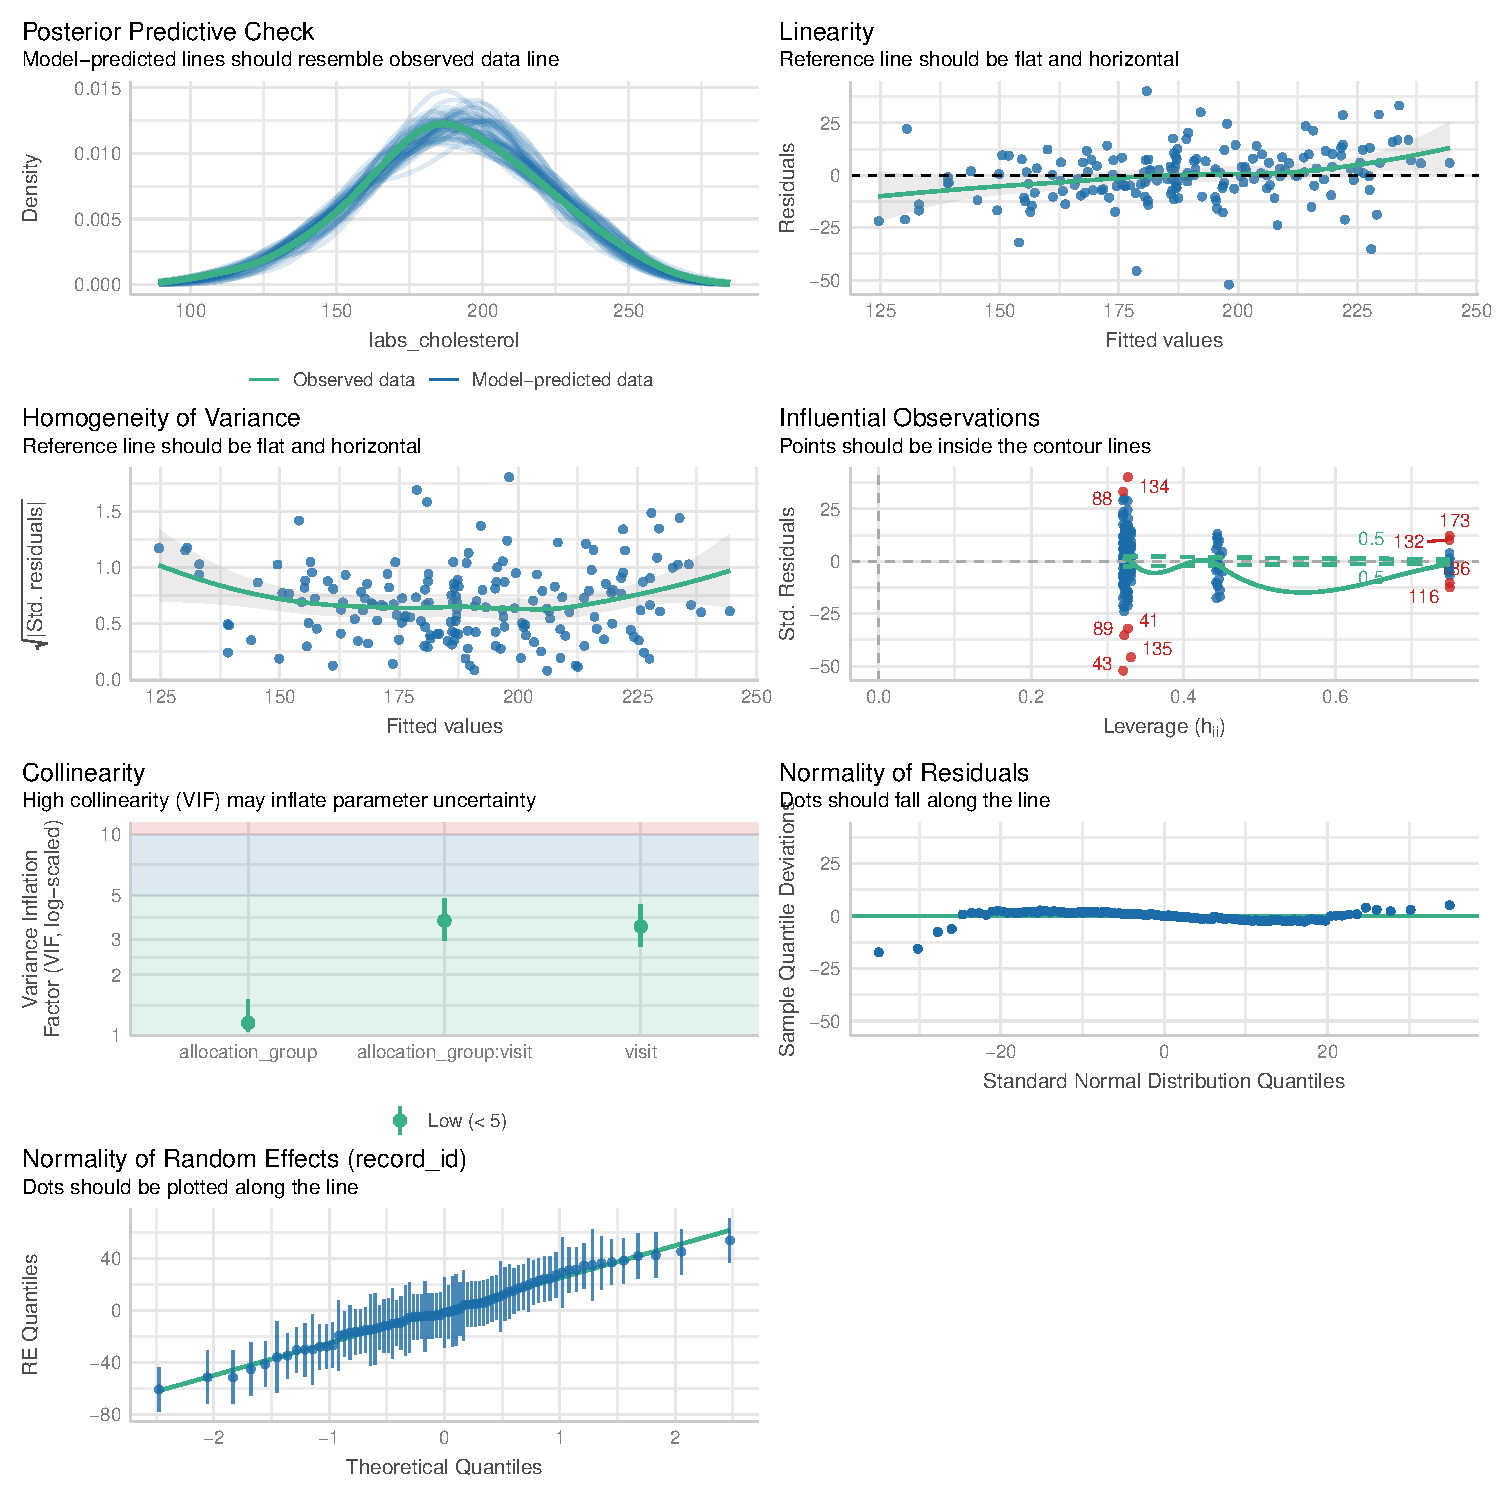
\includegraphics{Outcomes_V1V2V3_files/figure-pdf/labs_cholesterol_4-1.pdf}

\begin{Shaded}
\begin{Highlighting}[]
\NormalTok{performance}\SpecialCharTok{::}\FunctionTok{check\_model}\NormalTok{(labs\_cholesterol\_model\_sens)}
\end{Highlighting}
\end{Shaded}

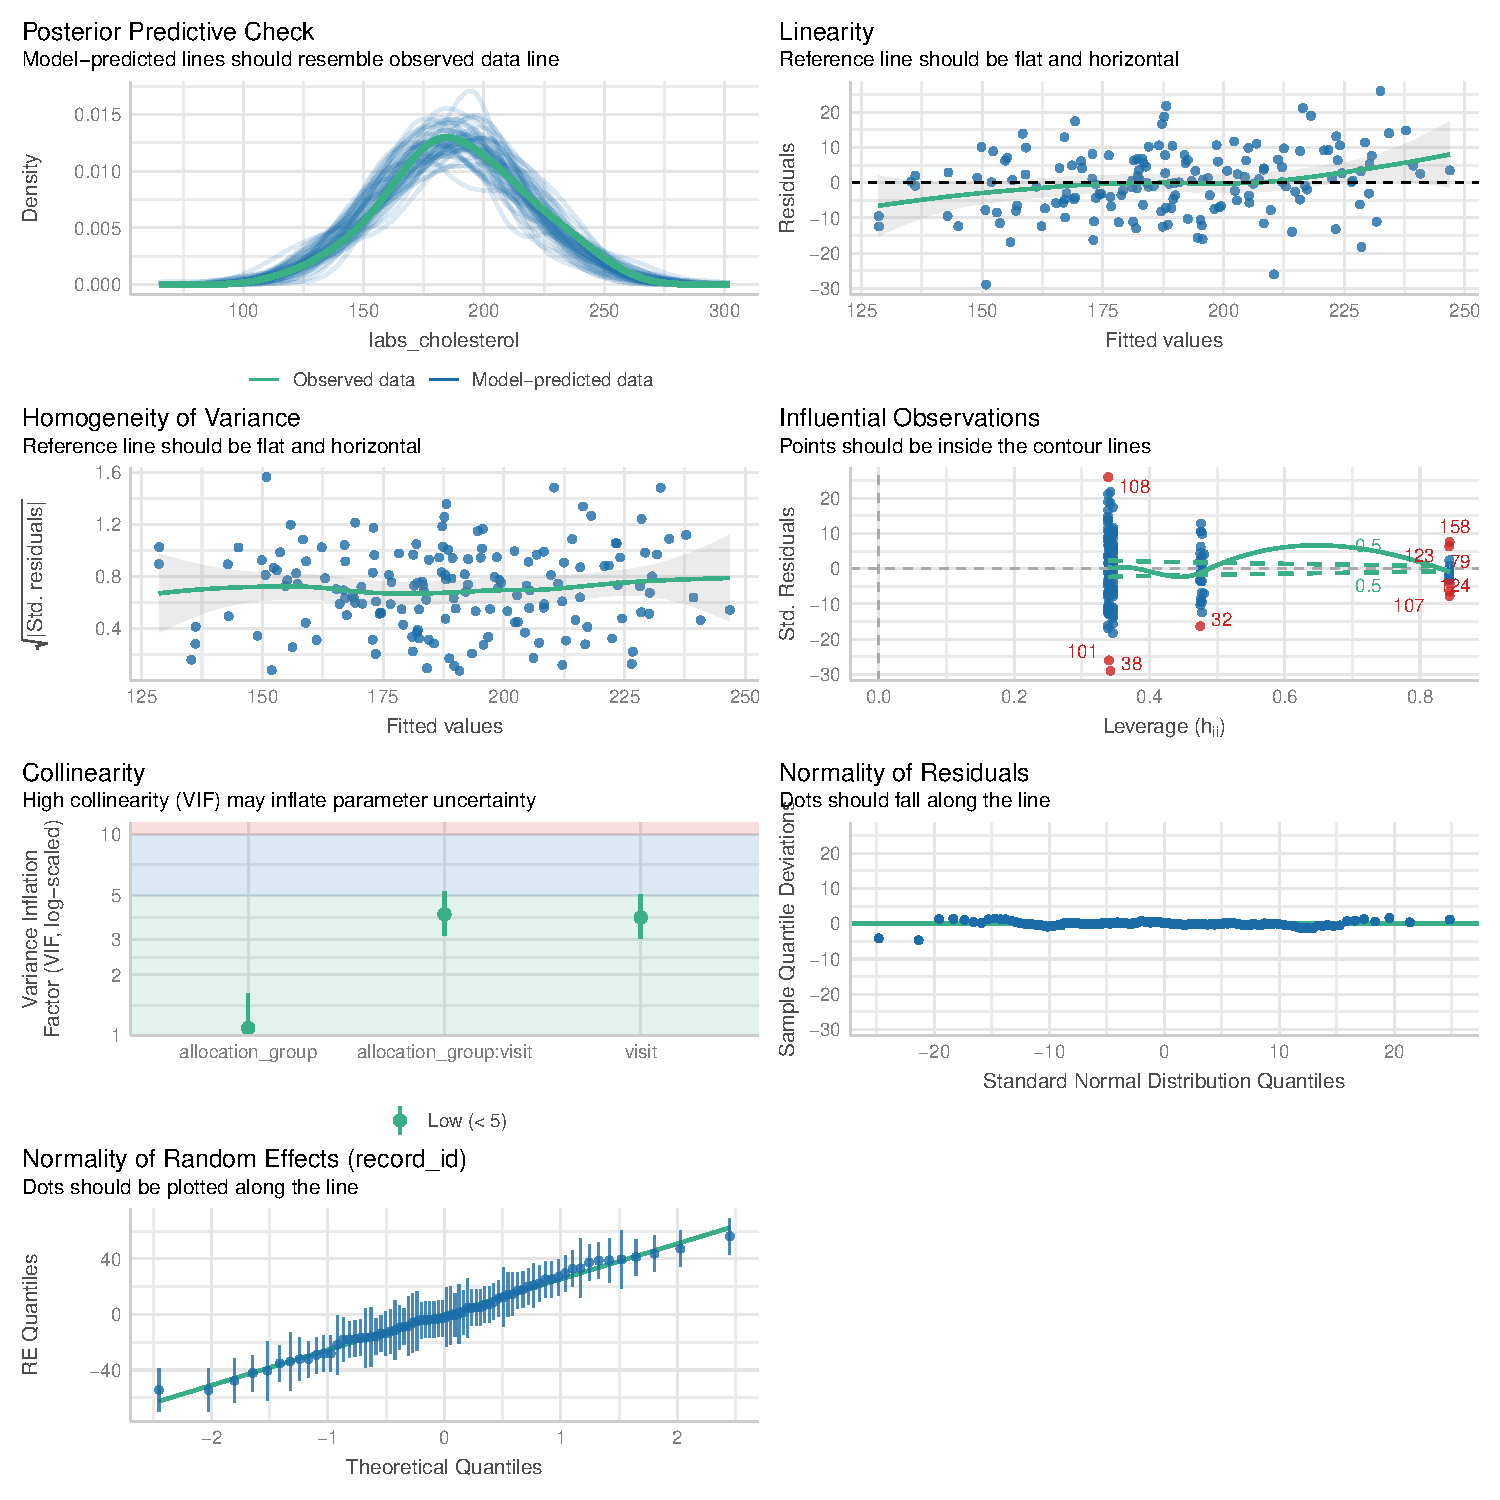
\includegraphics{Outcomes_V1V2V3_files/figure-pdf/labs_cholesterol_4-2.pdf}

\paragraph{Médias Marginais
Estimadas}\label{muxe9dias-marginais-estimadas-4}

\begin{Shaded}
\begin{Highlighting}[]
\CommentTok{\# Get EMMs for each group at each visit}
\NormalTok{labs\_cholesterol\_raw\_emm }\OtherTok{\textless{}{-}}\NormalTok{ emmeans}\SpecialCharTok{::}\FunctionTok{emmeans}\NormalTok{(}
\NormalTok{    labs\_cholesterol\_model, }
    \SpecialCharTok{\textasciitilde{}}\NormalTok{ allocation\_group }\SpecialCharTok{*}\NormalTok{ visit}
\NormalTok{)}

\NormalTok{labs\_cholesterol\_raw\_emm }\OtherTok{\textless{}{-}} \FunctionTok{regrid}\NormalTok{(labs\_cholesterol\_raw\_emm)}

\CommentTok{\# Table of marginal means}
\NormalTok{labs\_cholesterol\_raw\_emm}
\end{Highlighting}
\end{Shaded}

\begin{verbatim}
 allocation_group visit emmean   SE    df lower.CL upper.CL
 Grupo A          1        191 5.20  95.4      181      202
 Grupo B          1        191 5.13  95.4      180      201
 Grupo A          2        185 5.42 107.2      175      196
 Grupo B          2        184 5.62 121.6      173      196
 Grupo A          3        191 5.68 121.8      180      202
 Grupo B          3        182 5.85 133.4      171      194

Degrees-of-freedom method: inherited from kenward-roger when re-gridding 
Confidence level used: 0.95 
\end{verbatim}

\begin{Shaded}
\begin{Highlighting}[]
\CommentTok{\# Pairwise comparisons: Between groups at each visit}
\NormalTok{emmeans}\SpecialCharTok{::}\FunctionTok{contrast}\NormalTok{(labs\_cholesterol\_raw\_emm, }\AttributeTok{method =} \StringTok{"pairwise"}\NormalTok{, }\AttributeTok{by =} \StringTok{"visit"}\NormalTok{, }\AttributeTok{adjust =} \StringTok{"bonferroni"}\NormalTok{) }\SpecialCharTok{\%\textgreater{}\%} \FunctionTok{summary}\NormalTok{(}\AttributeTok{infer =} \FunctionTok{c}\NormalTok{(}\ConstantTok{TRUE}\NormalTok{, }\ConstantTok{TRUE}\NormalTok{))}
\end{Highlighting}
\end{Shaded}

\begin{verbatim}
visit = 1:
 contrast          estimate   SE    df lower.CL upper.CL t.ratio p.value
 Grupo A - Grupo B    0.717 7.30  95.4   -13.78     15.2   0.098  0.9221

visit = 2:
 contrast          estimate   SE    df lower.CL upper.CL t.ratio p.value
 Grupo A - Grupo B    0.832 7.81 107.2   -14.65     16.3   0.107  0.9154

visit = 3:
 contrast          estimate   SE    df lower.CL upper.CL t.ratio p.value
 Grupo A - Grupo B    8.476 8.15 121.8    -7.66     24.6   1.040  0.3004

Degrees-of-freedom method: inherited from kenward-roger when re-gridding 
Confidence level used: 0.95 
\end{verbatim}

\begin{Shaded}
\begin{Highlighting}[]
\CommentTok{\# Pairwise comparisons: Changes over time within each group}
\NormalTok{emmeans}\SpecialCharTok{::}\FunctionTok{contrast}\NormalTok{(labs\_cholesterol\_raw\_emm, }\AttributeTok{method =} \StringTok{"pairwise"}\NormalTok{, }\AttributeTok{by =} \StringTok{"allocation\_group"}\NormalTok{, }\AttributeTok{adjust =} \StringTok{"bonferroni"}\NormalTok{) }\SpecialCharTok{\%\textgreater{}\%} \FunctionTok{summary}\NormalTok{(}\AttributeTok{infer =} \FunctionTok{c}\NormalTok{(}\ConstantTok{TRUE}\NormalTok{, }\ConstantTok{TRUE}\NormalTok{))}
\end{Highlighting}
\end{Shaded}

\begin{verbatim}
allocation_group = Grupo A:
 contrast        estimate   SE    df lower.CL upper.CL t.ratio p.value
 visit1 - visit2     5.91 4.03  95.4    -3.92    15.73   1.465  0.4387
 visit1 - visit3     0.38 4.37  95.4   -10.27    11.03   0.087  1.0000
 visit2 - visit3    -5.53 4.41 107.2   -16.25     5.19  -1.254  0.6378

allocation_group = Grupo B:
 contrast        estimate   SE    df lower.CL upper.CL t.ratio p.value
 visit1 - visit2     6.02 4.34  95.4    -4.54    16.59   1.389  0.5041
 visit1 - visit3     8.14 4.62  95.4    -3.13    19.41   1.760  0.2448
 visit2 - visit3     2.12 4.82 121.6    -9.58    13.81   0.439  1.0000

Degrees-of-freedom method: inherited from kenward-roger when re-gridding 
Confidence level used: 0.95 
Conf-level adjustment: bonferroni method for 3 estimates 
P value adjustment: bonferroni method for 3 tests 
\end{verbatim}

\begin{Shaded}
\begin{Highlighting}[]
\CommentTok{\# Plot of marginal means}
\FunctionTok{plot}\NormalTok{(labs\_cholesterol\_raw\_emm, }\AttributeTok{comparisons =} \ConstantTok{TRUE}\NormalTok{)}
\end{Highlighting}
\end{Shaded}

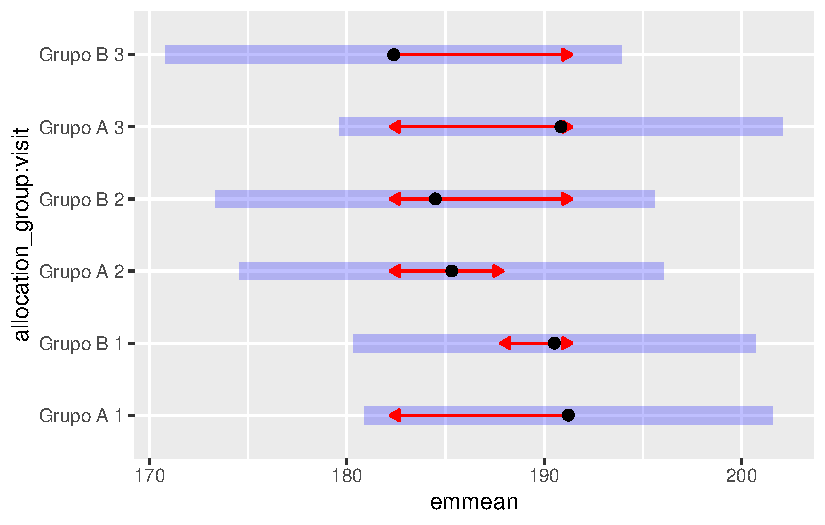
\includegraphics{Outcomes_V1V2V3_files/figure-pdf/labs_cholesterol_raw_emm-1.pdf}

\begin{Shaded}
\begin{Highlighting}[]
\CommentTok{\# Get EMMs for each group at each visit}
\NormalTok{labs\_cholesterol\_emm }\OtherTok{\textless{}{-}}\NormalTok{ emmeans}\SpecialCharTok{::}\FunctionTok{emmeans}\NormalTok{(}
\NormalTok{    labs\_cholesterol\_model\_sens, }
    \SpecialCharTok{\textasciitilde{}}\NormalTok{ allocation\_group }\SpecialCharTok{*}\NormalTok{ visit}
\NormalTok{)}

\NormalTok{labs\_cholesterol\_emm }\OtherTok{\textless{}{-}} \FunctionTok{regrid}\NormalTok{(labs\_cholesterol\_emm)}

\CommentTok{\# Table of marginal means}
\NormalTok{labs\_cholesterol\_emm}
\end{Highlighting}
\end{Shaded}

\begin{verbatim}
 allocation_group visit emmean   SE    df lower.CL upper.CL
 Grupo A          1        191 5.13  79.8      181      201
 Grupo B          1        190 4.84  79.8      181      200
 Grupo A          2        185 5.30  88.6      175      196
 Grupo B          2        183 5.16  97.7      173      193
 Grupo A          3        187 5.50  99.7      176      198
 Grupo B          3        184 5.31 106.3      174      195

Degrees-of-freedom method: inherited from kenward-roger when re-gridding 
Confidence level used: 0.95 
\end{verbatim}

\begin{Shaded}
\begin{Highlighting}[]
\CommentTok{\# Pairwise comparisons: Between groups at each visit}
\NormalTok{emmeans}\SpecialCharTok{::}\FunctionTok{contrast}\NormalTok{(labs\_cholesterol\_emm, }\AttributeTok{method =} \StringTok{"pairwise"}\NormalTok{, }\AttributeTok{by =} \StringTok{"visit"}\NormalTok{, }\AttributeTok{adjust =} \StringTok{"bonferroni"}\NormalTok{) }\SpecialCharTok{\%\textgreater{}\%} \FunctionTok{summary}\NormalTok{(}\AttributeTok{infer =} \FunctionTok{c}\NormalTok{(}\ConstantTok{TRUE}\NormalTok{, }\ConstantTok{TRUE}\NormalTok{))}
\end{Highlighting}
\end{Shaded}

\begin{verbatim}
visit = 1:
 contrast          estimate   SE   df lower.CL upper.CL t.ratio p.value
 Grupo A - Grupo B    0.678 7.05 79.8    -13.4     14.7   0.096  0.9237

visit = 2:
 contrast          estimate   SE   df lower.CL upper.CL t.ratio p.value
 Grupo A - Grupo B    2.235 7.40 88.6    -12.5     16.9   0.302  0.7632

visit = 3:
 contrast          estimate   SE   df lower.CL upper.CL t.ratio p.value
 Grupo A - Grupo B    2.807 7.64 99.7    -12.4     18.0   0.367  0.7142

Degrees-of-freedom method: inherited from kenward-roger when re-gridding 
Confidence level used: 0.95 
\end{verbatim}

\begin{Shaded}
\begin{Highlighting}[]
\CommentTok{\# Pairwise comparisons: Changes over time within each group}
\NormalTok{emmeans}\SpecialCharTok{::}\FunctionTok{contrast}\NormalTok{(labs\_cholesterol\_emm, }\AttributeTok{method =} \StringTok{"pairwise"}\NormalTok{, }\AttributeTok{by =} \StringTok{"allocation\_group"}\NormalTok{, }\AttributeTok{adjust =} \StringTok{"bonferroni"}\NormalTok{) }\SpecialCharTok{\%\textgreater{}\%} \FunctionTok{summary}\NormalTok{(}\AttributeTok{infer =} \FunctionTok{c}\NormalTok{(}\ConstantTok{TRUE}\NormalTok{, }\ConstantTok{TRUE}\NormalTok{))}
\end{Highlighting}
\end{Shaded}

\begin{verbatim}
allocation_group = Grupo A:
 contrast        estimate   SE   df lower.CL upper.CL t.ratio p.value
 visit1 - visit2     5.98 3.20 79.8   -1.832    13.80   1.872  0.1944
 visit1 - visit3     3.94 3.52 79.8   -4.665    12.54   1.119  0.7990
 visit2 - visit3    -2.05 3.54 88.6  -10.679     6.59  -0.579  1.0000

allocation_group = Grupo B:
 contrast        estimate   SE   df lower.CL upper.CL t.ratio p.value
 visit1 - visit2     7.54 3.28 79.8   -0.478    15.56   2.300  0.0723
 visit1 - visit3     6.07 3.51 79.8   -2.516    14.65   1.729  0.2632
 visit2 - visit3    -1.47 3.65 97.7  -10.355     7.41  -0.404  1.0000

Degrees-of-freedom method: inherited from kenward-roger when re-gridding 
Confidence level used: 0.95 
Conf-level adjustment: bonferroni method for 3 estimates 
P value adjustment: bonferroni method for 3 tests 
\end{verbatim}

\begin{Shaded}
\begin{Highlighting}[]
\CommentTok{\# Plot of marginal means}
\FunctionTok{plot}\NormalTok{(labs\_cholesterol\_emm, }\AttributeTok{comparisons =} \ConstantTok{TRUE}\NormalTok{)}
\end{Highlighting}
\end{Shaded}

\begin{verbatim}
Warning: Comparison discrepancy in group "1", Grupo B visit1 - Grupo A visit2:
    Target overlap = 0.7468, overlap on graph = -1.2872
\end{verbatim}

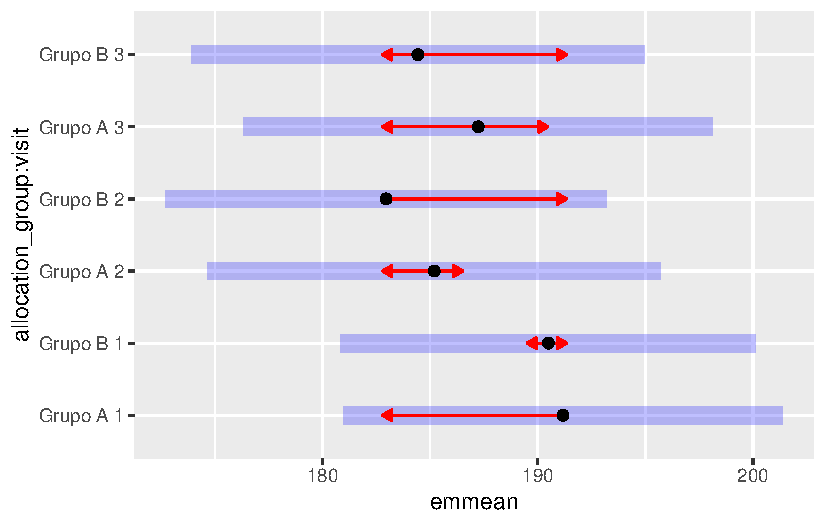
\includegraphics{Outcomes_V1V2V3_files/figure-pdf/labs_cholesterol_sens_emm-1.pdf}

\begin{Shaded}
\begin{Highlighting}[]
\FunctionTok{ggplot}\NormalTok{(}
    \AttributeTok{data =}\NormalTok{ data\_model, }
    \FunctionTok{aes}\NormalTok{(}
        \AttributeTok{x =} \FunctionTok{as.factor}\NormalTok{(visit),}
        \AttributeTok{y =}\NormalTok{ labs\_cholesterol,}
        \AttributeTok{group =}\NormalTok{ record\_id,}
\NormalTok{    )}
\NormalTok{) }\SpecialCharTok{+}
    \FunctionTok{geom\_line}\NormalTok{(}\AttributeTok{alpha =} \FloatTok{0.5}\NormalTok{) }\SpecialCharTok{+}
    \FunctionTok{geom\_point}\NormalTok{(}\AttributeTok{alpha =} \FloatTok{0.7}\NormalTok{) }\SpecialCharTok{+}
    \FunctionTok{geom\_smooth}\NormalTok{(}
        \FunctionTok{aes}\NormalTok{(}\AttributeTok{group =}\NormalTok{ allocation\_group),}
        \AttributeTok{method =} \StringTok{"lm"}\NormalTok{,}
        \AttributeTok{se =} \ConstantTok{TRUE}\NormalTok{,}
        \AttributeTok{linewidth =} \DecValTok{1}
\NormalTok{    ) }\SpecialCharTok{+}
    \FunctionTok{labs}\NormalTok{(}\AttributeTok{title =} \StringTok{"All data"}\NormalTok{) }\SpecialCharTok{+}
    \FunctionTok{facet\_wrap}\NormalTok{(}\SpecialCharTok{\textasciitilde{}}\NormalTok{ allocation\_group) }
\end{Highlighting}
\end{Shaded}

\begin{verbatim}
`geom_smooth()` using formula = 'y ~ x'
\end{verbatim}

\begin{verbatim}
Warning: Removed 10 rows containing non-finite outside the scale range
(`stat_smooth()`).
\end{verbatim}

\begin{verbatim}
Warning: Removed 8 rows containing missing values or values outside the scale range
(`geom_line()`).
\end{verbatim}

\begin{verbatim}
Warning: Removed 10 rows containing missing values or values outside the scale range
(`geom_point()`).
\end{verbatim}

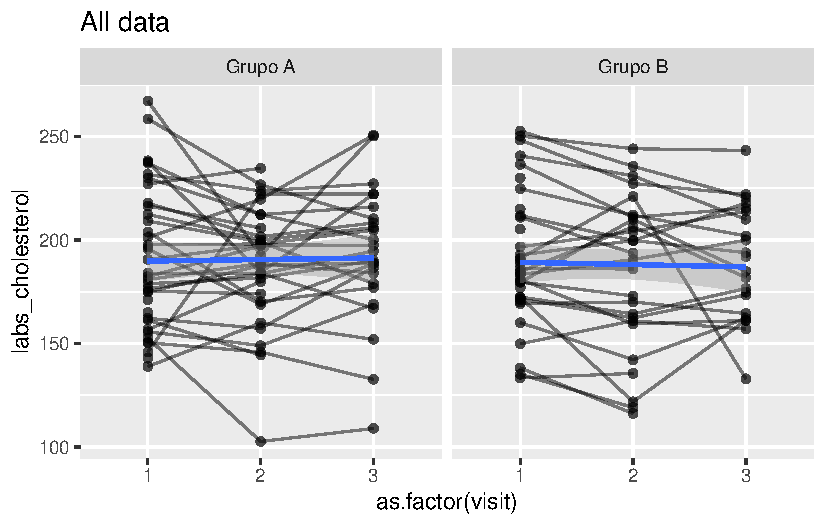
\includegraphics{Outcomes_V1V2V3_files/figure-pdf/labs_cholesterol_6-1.pdf}

\begin{Shaded}
\begin{Highlighting}[]
    \CommentTok{\#coord\_cartesian(ylim = c(10, 150))}

\NormalTok{data\_model }\SpecialCharTok{\%\textgreater{}\%} 
    \FunctionTok{filter}\NormalTok{(}
        \SpecialCharTok{!}\NormalTok{(record\_id }\SpecialCharTok{\%in\%}\NormalTok{ labs\_cholesterol\_model\_check}\SpecialCharTok{$}\NormalTok{influential\_ids)}
\NormalTok{    ) }\SpecialCharTok{\%\textgreater{}\%} 
    \FunctionTok{ggplot}\NormalTok{(}
        \FunctionTok{aes}\NormalTok{(}
            \AttributeTok{x =} \FunctionTok{as.factor}\NormalTok{(visit),}
            \AttributeTok{y =}\NormalTok{ labs\_cholesterol,}
            \AttributeTok{group =}\NormalTok{ record\_id,}
\NormalTok{        )}
\NormalTok{    ) }\SpecialCharTok{+}
    \FunctionTok{geom\_line}\NormalTok{(}\AttributeTok{alpha =} \FloatTok{0.5}\NormalTok{) }\SpecialCharTok{+}
    \FunctionTok{geom\_point}\NormalTok{(}\AttributeTok{alpha =} \FloatTok{0.7}\NormalTok{) }\SpecialCharTok{+}
    \FunctionTok{geom\_smooth}\NormalTok{(}
        \FunctionTok{aes}\NormalTok{(}\AttributeTok{group =}\NormalTok{ allocation\_group),}
        \AttributeTok{method =} \StringTok{"lm"}\NormalTok{,}
        \AttributeTok{se =} \ConstantTok{TRUE}\NormalTok{,}
        \AttributeTok{linewidth =} \DecValTok{1}
\NormalTok{    ) }\SpecialCharTok{+}
    \FunctionTok{labs}\NormalTok{(}\AttributeTok{title =} \StringTok{"Sensitivity analysis"}\NormalTok{) }\SpecialCharTok{+}
    \FunctionTok{facet\_wrap}\NormalTok{(}\SpecialCharTok{\textasciitilde{}}\NormalTok{ allocation\_group) }
\end{Highlighting}
\end{Shaded}

\begin{verbatim}
`geom_smooth()` using formula = 'y ~ x'
\end{verbatim}

\begin{verbatim}
Warning: Removed 10 rows containing non-finite outside the scale range
(`stat_smooth()`).
\end{verbatim}

\begin{verbatim}
Warning: Removed 8 rows containing missing values or values outside the scale range
(`geom_line()`).
\end{verbatim}

\begin{verbatim}
Warning: Removed 10 rows containing missing values or values outside the scale range
(`geom_point()`).
\end{verbatim}

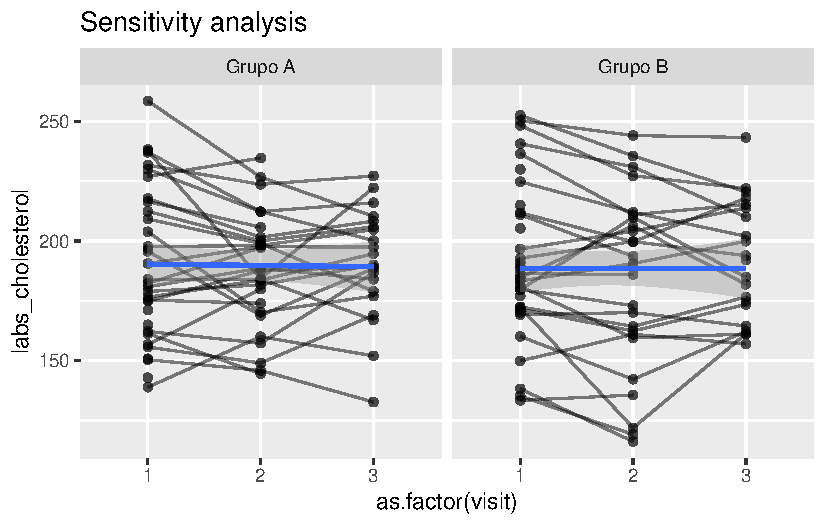
\includegraphics{Outcomes_V1V2V3_files/figure-pdf/labs_cholesterol_6-2.pdf}

\begin{Shaded}
\begin{Highlighting}[]
    \CommentTok{\#coord\_cartesian(ylim = c(10, 150))}
\end{Highlighting}
\end{Shaded}

\subsubsection{LDL Colesterol}\label{ldl-colesterol}

Variável: \texttt{labs\_ldl}

\begin{Shaded}
\begin{Highlighting}[]
\CommentTok{\# Plot 1: Raw data}
\NormalTok{labs\_ldl\_hist\_1 }\OtherTok{\textless{}{-}}\NormalTok{ data\_model }\SpecialCharTok{\%\textgreater{}\%} 
    \CommentTok{\#filter(}
    \CommentTok{\#    labs\_ldl \textless{} 300}
    \CommentTok{\#) \%\textgreater{}\% }
    \FunctionTok{ggplot}\NormalTok{(}\FunctionTok{aes}\NormalTok{(}\AttributeTok{x =}\NormalTok{ labs\_ldl)) }\SpecialCharTok{+} 
    \FunctionTok{geom\_histogram}\NormalTok{(}\AttributeTok{bins =} \DecValTok{50}\NormalTok{, }\AttributeTok{fill =} \StringTok{"skyblue"}\NormalTok{, }\AttributeTok{color =} \StringTok{"black"}\NormalTok{)}

\CommentTok{\# Plot 2: Log{-}transformed data}
\NormalTok{labs\_ldl\_hist\_2 }\OtherTok{\textless{}{-}}\NormalTok{ data\_model }\SpecialCharTok{\%\textgreater{}\%} 
    \CommentTok{\#filter(}
    \CommentTok{\#    labs\_ldl \textless{} 300}
    \CommentTok{\#) \%\textgreater{}\%}
    \FunctionTok{ggplot}\NormalTok{(}\FunctionTok{aes}\NormalTok{(}\AttributeTok{x =} \FunctionTok{log1p}\NormalTok{(labs\_ldl))) }\SpecialCharTok{+} 
    \FunctionTok{geom\_histogram}\NormalTok{(}\AttributeTok{bins =} \DecValTok{50}\NormalTok{, }\AttributeTok{fill =} \StringTok{"lightgreen"}\NormalTok{, }\AttributeTok{color =} \StringTok{"black"}\NormalTok{)}

\CommentTok{\# Combine side by side}
\NormalTok{labs\_ldl\_hist\_1 }\SpecialCharTok{+}\NormalTok{ labs\_ldl\_hist\_2 }\CommentTok{\# library(patchwork)}
\end{Highlighting}
\end{Shaded}

\begin{verbatim}
Warning: Removed 10 rows containing non-finite outside the scale range (`stat_bin()`).
Removed 10 rows containing non-finite outside the scale range (`stat_bin()`).
\end{verbatim}

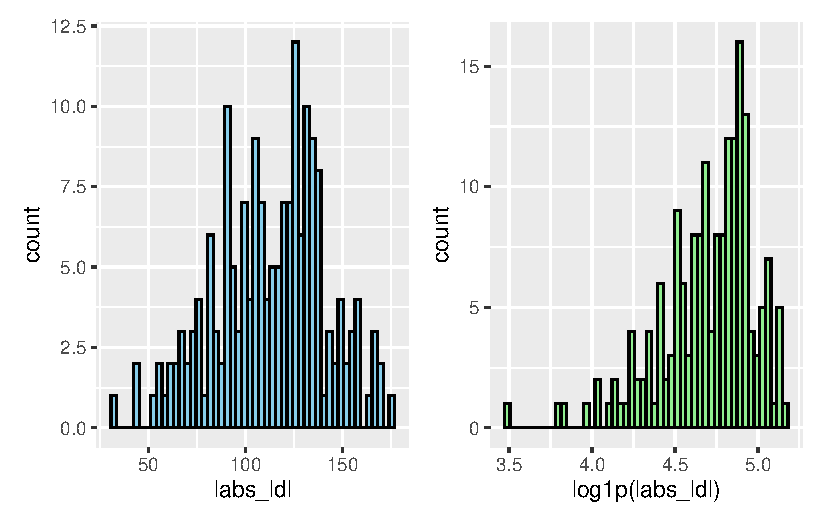
\includegraphics{Outcomes_V1V2V3_files/figure-pdf/labs_ldl_1-1.pdf}

\begin{Shaded}
\begin{Highlighting}[]
\CommentTok{\# LMM}
\NormalTok{labs\_ldl\_model }\OtherTok{\textless{}{-}} \FunctionTok{lmer}\NormalTok{(labs\_ldl }\SpecialCharTok{\textasciitilde{}}\NormalTok{ allocation\_group }\SpecialCharTok{*}\NormalTok{ visit }\SpecialCharTok{+}\NormalTok{ (}\DecValTok{1} \SpecialCharTok{|}\NormalTok{ record\_id), }\AttributeTok{data =}\NormalTok{ data\_model)}
\FunctionTok{check\_collinearity}\NormalTok{(labs\_ldl\_model)}
\end{Highlighting}
\end{Shaded}

\begin{verbatim}
# Check for Multicollinearity

Low Correlation

                   Term  VIF   VIF 95% CI Increased SE Tolerance
       allocation_group 1.18 [1.06, 1.52]         1.08      0.85
                  visit 3.49 [2.78, 4.49]         1.87      0.29
 allocation_group:visit 3.77 [3.00, 4.86]         1.94      0.26
 Tolerance 95% CI
     [0.66, 0.94]
     [0.22, 0.36]
     [0.21, 0.33]
\end{verbatim}

\begin{Shaded}
\begin{Highlighting}[]
\CommentTok{\# Sensitivity analysis}
\NormalTok{labs\_ldl\_model\_check }\OtherTok{\textless{}{-}} \FunctionTok{sensitivity\_check\_lmer}\NormalTok{(}
    \AttributeTok{model =}\NormalTok{ labs\_ldl\_model,}
    \AttributeTok{id\_var =} \StringTok{"record\_id"}\NormalTok{,}
    \AttributeTok{top\_n =} \DecValTok{5}\NormalTok{)}

\CommentTok{\# LMM Sensitivity}
\NormalTok{labs\_ldl\_model\_sens }\OtherTok{\textless{}{-}} \FunctionTok{update}\NormalTok{(}\AttributeTok{object =}\NormalTok{ labs\_ldl\_model,}
                              \AttributeTok{subset =} \SpecialCharTok{!}\NormalTok{(record\_id }\SpecialCharTok{\%in\%}\NormalTok{ labs\_ldl\_model\_check}\SpecialCharTok{$}\NormalTok{influential\_ids))}
\CommentTok{\# Influential IDS}
\NormalTok{labs\_ldl\_model\_check}\SpecialCharTok{$}\NormalTok{influential\_ids}
\end{Highlighting}
\end{Shaded}

\begin{verbatim}
[1] "16" "17" "56" "37" "50"
\end{verbatim}

\paragraph{Resumo dos modelos}\label{resumo-dos-modelos-5}

\begin{Shaded}
\begin{Highlighting}[]
\CommentTok{\# Model comparison}
\FunctionTok{summary}\NormalTok{(labs\_ldl\_model)}
\end{Highlighting}
\end{Shaded}

\begin{verbatim}
Linear mixed model fit by REML. t-tests use Satterthwaite's method [
lmerModLmerTest]
Formula: labs_ldl ~ allocation_group * visit + (1 | record_id)
   Data: data_model

REML criterion at convergence: 1601.5

Scaled residuals: 
    Min      1Q  Median      3Q     Max 
-2.9892 -0.3229 -0.0296  0.3610  2.5195 

Random effects:
 Groups    Name        Variance Std.Dev.
 record_id (Intercept) 605.7    24.61   
 Residual              249.7    15.80   
Number of obs: 179, groups:  record_id, 75

Fixed effects:
                               Estimate Std. Error       df t value Pr(>|t|)
(Intercept)                    115.4919     4.8081  98.3445  24.020   <2e-16
allocation_groupGrupo B         -3.7735     6.7548  98.3445  -0.559    0.578
visit2                          -5.5925     3.9659 103.9503  -1.410    0.161
visit3                          -0.0205     4.2968 105.1671  -0.005    0.996
allocation_groupGrupo B:visit2   1.9191     5.8182 105.6037   0.330    0.742
allocation_groupGrupo B:visit3  -5.9060     6.2502 106.5086  -0.945    0.347
                                  
(Intercept)                    ***
allocation_groupGrupo B           
visit2                            
visit3                            
allocation_groupGrupo B:visit2    
allocation_groupGrupo B:visit3    
---
Signif. codes:  0 '***' 0.001 '**' 0.01 '*' 0.05 '.' 0.1 ' ' 1

Correlation of Fixed Effects:
            (Intr) all_GB visit2 visit3 a_GB:2
allctn_grGB -0.712                            
visit2      -0.354  0.252                     
visit3      -0.327  0.233  0.450              
allctn_GB:2  0.241 -0.339 -0.682 -0.307       
allctn_GB:3  0.225 -0.315 -0.310 -0.687  0.434
\end{verbatim}

\begin{Shaded}
\begin{Highlighting}[]
\FunctionTok{summary}\NormalTok{(labs\_ldl\_model\_sens)}
\end{Highlighting}
\end{Shaded}

\begin{verbatim}
Linear mixed model fit by REML. t-tests use Satterthwaite's method [
lmerModLmerTest]
Formula: labs_ldl ~ allocation_group * visit + (1 | record_id)
   Data: data_model
 Subset: !(record_id %in% labs_ldl_model_check$influential_ids)

REML criterion at convergence: 1409.6

Scaled residuals: 
     Min       1Q   Median       3Q      Max 
-2.40389 -0.45872 -0.04587  0.38702  2.26265 

Random effects:
 Groups    Name        Variance Std.Dev.
 record_id (Intercept) 663.1    25.75   
 Residual              134.9    11.61   
Number of obs: 164, groups:  record_id, 70

Fixed effects:
                               Estimate Std. Error       df t value Pr(>|t|)
(Intercept)                    113.7000     4.8448  79.8422  23.469   <2e-16
allocation_groupGrupo B         -1.6611     6.7557  79.8422  -0.246    0.806
visit2                          -4.7013     3.0810  92.0892  -1.526    0.130
visit3                          -0.1022     3.3768  92.6447  -0.030    0.976
allocation_groupGrupo B:visit2   1.4048     4.5009  92.9553   0.312    0.756
allocation_groupGrupo B:visit3  -4.6904     4.8797  93.3370  -0.961    0.339
                                  
(Intercept)                    ***
allocation_groupGrupo B           
visit2                            
visit3                            
allocation_groupGrupo B:visit2    
allocation_groupGrupo B:visit3    
---
Signif. codes:  0 '***' 0.001 '**' 0.01 '*' 0.05 '.' 0.1 ' ' 1

Correlation of Fixed Effects:
            (Intr) all_GB visit2 visit3 a_GB:2
allctn_grGB -0.717                            
visit2      -0.266  0.191                     
visit3      -0.243  0.174  0.449              
allctn_GB:2  0.182 -0.254 -0.685 -0.308       
allctn_GB:3  0.168 -0.234 -0.311 -0.692  0.434
\end{verbatim}

\begin{Shaded}
\begin{Highlighting}[]
\NormalTok{labs\_ldl\_model\_check}\SpecialCharTok{$}\NormalTok{comparison\_table}
\end{Highlighting}
\end{Shaded}

\begin{verbatim}
# A tibble: 16 x 6
   Model       term                       estimate std.error statistic   p.value
   <chr>       <chr>                         <dbl>     <dbl>     <dbl>     <dbl>
 1 Original    (Intercept)                115.          4.81  24.0      6.20e-43
 2 Sensitivity (Intercept)                114.          4.84  23.5      1.40e-37
 3 Original    allocation_groupGrupo B     -3.77        6.75  -0.559    5.78e- 1
 4 Sensitivity allocation_groupGrupo B     -1.66        6.76  -0.246    8.06e- 1
 5 Original    allocation_groupGrupo B:v~   1.92        5.82   0.330    7.42e- 1
 6 Sensitivity allocation_groupGrupo B:v~   1.40        4.50   0.312    7.56e- 1
 7 Original    allocation_groupGrupo B:v~  -5.91        6.25  -0.945    3.47e- 1
 8 Sensitivity allocation_groupGrupo B:v~  -4.69        4.88  -0.961    3.39e- 1
 9 Original    sd__(Intercept)             24.6        NA     NA       NA       
10 Sensitivity sd__(Intercept)             25.8        NA     NA       NA       
11 Original    sd__Observation             15.8        NA     NA       NA       
12 Sensitivity sd__Observation             11.6        NA     NA       NA       
13 Original    visit2                      -5.59        3.97  -1.41     1.61e- 1
14 Sensitivity visit2                      -4.70        3.08  -1.53     1.30e- 1
15 Original    visit3                      -0.0205      4.30  -0.00477  9.96e- 1
16 Sensitivity visit3                      -0.102       3.38  -0.0303   9.76e- 1
\end{verbatim}

\begin{Shaded}
\begin{Highlighting}[]
\NormalTok{performance}\SpecialCharTok{::}\FunctionTok{compare\_performance}\NormalTok{(labs\_ldl\_model, labs\_ldl\_model\_sens)}
\end{Highlighting}
\end{Shaded}

\begin{verbatim}
When comparing models, please note that probably not all models were fit
  from same data.
\end{verbatim}

\begin{verbatim}
# Comparison of Model Performance Indices

Name                |           Model |  AIC (weights) | AICc (weights)
-----------------------------------------------------------------------
labs_ldl_model      | lmerModLmerTest | 1645.5 (<.001) | 1646.4 (<.001)
labs_ldl_model_sens | lmerModLmerTest | 1451.7 (>.999) | 1452.6 (>.999)

Name                |  BIC (weights) | R2 (cond.) | R2 (marg.) |   ICC |   RMSE |  Sigma
----------------------------------------------------------------------------------------
labs_ldl_model      | 1671.0 (<.001) |      0.712 |      0.014 | 0.708 | 12.514 | 15.802
labs_ldl_model_sens | 1476.5 (>.999) |      0.832 |      0.007 | 0.831 |  8.905 | 11.615
\end{verbatim}

\begin{Shaded}
\begin{Highlighting}[]
\NormalTok{performance}\SpecialCharTok{::}\FunctionTok{check\_model}\NormalTok{(labs\_ldl\_model)}
\end{Highlighting}
\end{Shaded}

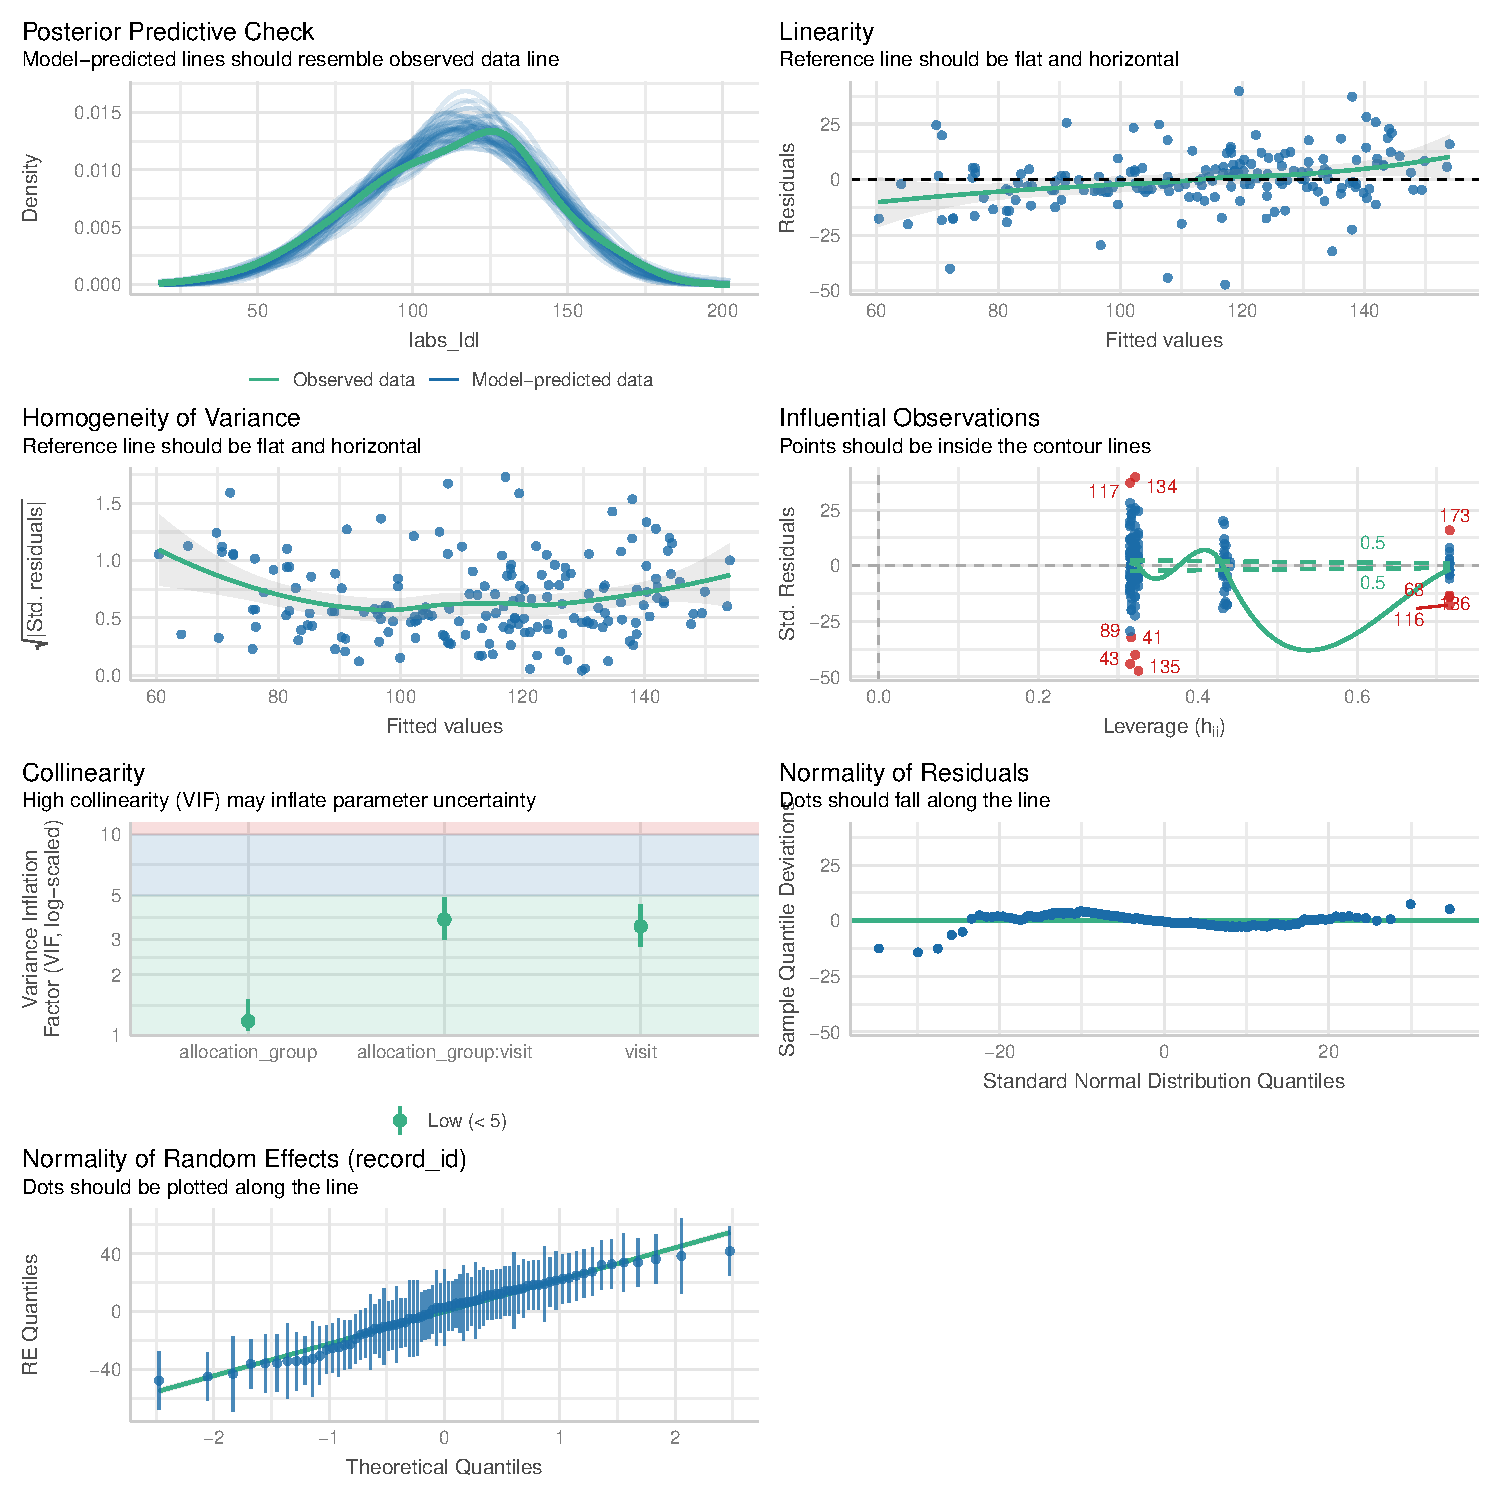
\includegraphics{Outcomes_V1V2V3_files/figure-pdf/labs_ldl_4-1.pdf}

\begin{Shaded}
\begin{Highlighting}[]
\NormalTok{performance}\SpecialCharTok{::}\FunctionTok{check\_model}\NormalTok{(labs\_ldl\_model\_sens)}
\end{Highlighting}
\end{Shaded}

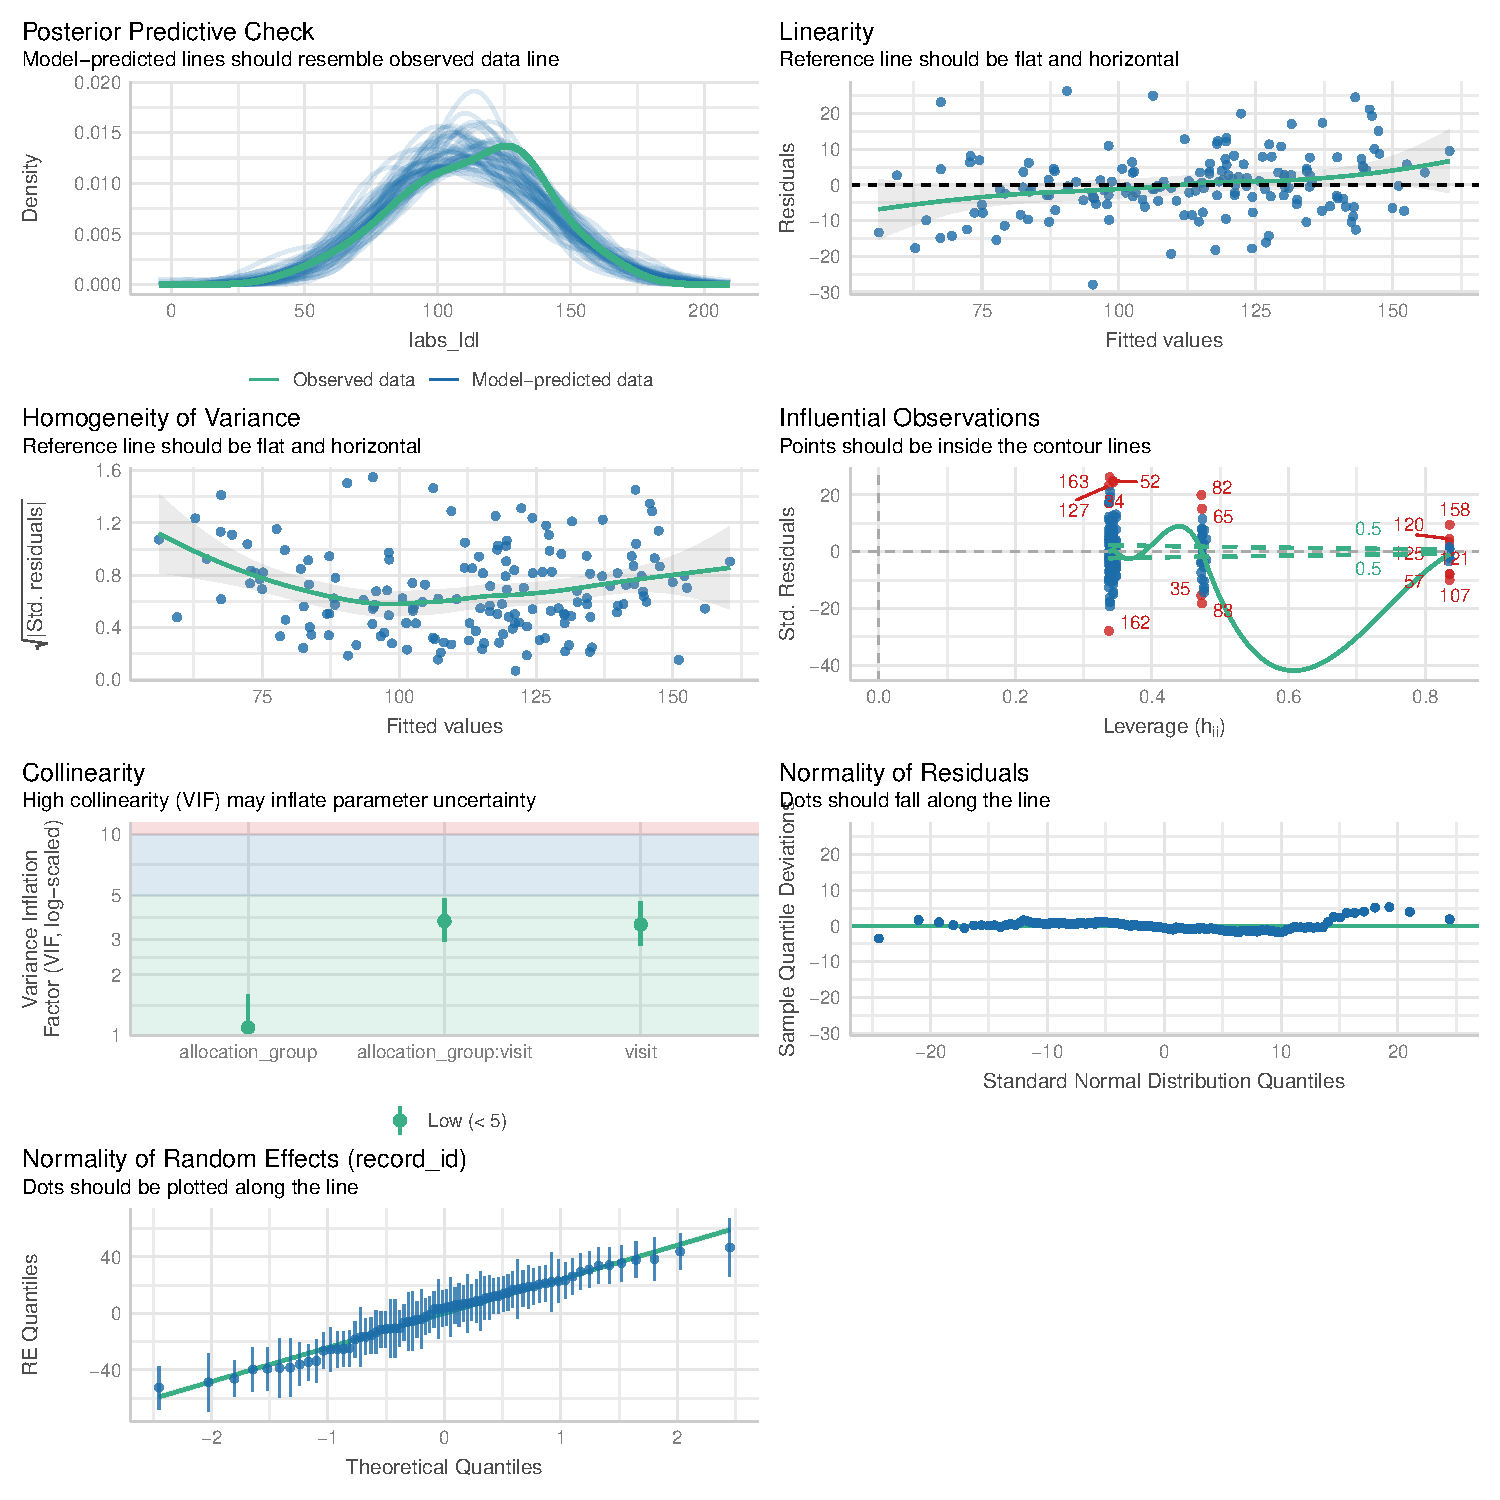
\includegraphics{Outcomes_V1V2V3_files/figure-pdf/labs_ldl_4-2.pdf}

\paragraph{Médias Marginais
Estimadas}\label{muxe9dias-marginais-estimadas-5}

\begin{Shaded}
\begin{Highlighting}[]
\CommentTok{\# Get EMMs for each group at each visit}
\NormalTok{labs\_ldl\_raw\_emm }\OtherTok{\textless{}{-}}\NormalTok{ emmeans}\SpecialCharTok{::}\FunctionTok{emmeans}\NormalTok{(}
\NormalTok{    labs\_ldl\_model, }
    \SpecialCharTok{\textasciitilde{}}\NormalTok{ allocation\_group }\SpecialCharTok{*}\NormalTok{ visit}
\NormalTok{)}

\NormalTok{labs\_ldl\_raw\_emm }\OtherTok{\textless{}{-}} \FunctionTok{regrid}\NormalTok{(labs\_ldl\_raw\_emm)}

\CommentTok{\# Table of marginal means}
\NormalTok{labs\_ldl\_raw\_emm}
\end{Highlighting}
\end{Shaded}

\begin{verbatim}
 allocation_group visit emmean   SE    df lower.CL upper.CL
 Grupo A          1        115 4.81  99.1    106.0      125
 Grupo B          1        112 4.74  99.1    102.3      121
 Grupo A          2        110 5.04 111.9     99.9      120
 Grupo B          2        108 5.25 127.2     97.7      118
 Grupo A          3        115 5.30 127.7    105.0      126
 Grupo B          3        106 5.48 139.4     95.0      117

Degrees-of-freedom method: inherited from kenward-roger when re-gridding 
Confidence level used: 0.95 
\end{verbatim}

\begin{Shaded}
\begin{Highlighting}[]
\CommentTok{\# Pairwise comparisons: Between groups at each visit}
\NormalTok{emmeans}\SpecialCharTok{::}\FunctionTok{contrast}\NormalTok{(labs\_ldl\_raw\_emm, }\AttributeTok{method =} \StringTok{"pairwise"}\NormalTok{, }\AttributeTok{by =} \StringTok{"visit"}\NormalTok{, }\AttributeTok{adjust =} \StringTok{"bonferroni"}\NormalTok{) }\SpecialCharTok{\%\textgreater{}\%} \FunctionTok{summary}\NormalTok{(}\AttributeTok{infer =} \FunctionTok{c}\NormalTok{(}\ConstantTok{TRUE}\NormalTok{, }\ConstantTok{TRUE}\NormalTok{))}
\end{Highlighting}
\end{Shaded}

\begin{verbatim}
visit = 1:
 contrast          estimate   SE    df lower.CL upper.CL t.ratio p.value
 Grupo A - Grupo B     3.77 6.75  99.1    -9.63     17.2   0.559  0.5777

visit = 2:
 contrast          estimate   SE    df lower.CL upper.CL t.ratio p.value
 Grupo A - Grupo B     1.85 7.27 111.9   -12.56     16.3   0.255  0.7993

visit = 3:
 contrast          estimate   SE    df lower.CL upper.CL t.ratio p.value
 Grupo A - Grupo B     9.68 7.63 127.7    -5.41     24.8   1.269  0.2067

Degrees-of-freedom method: inherited from kenward-roger when re-gridding 
Confidence level used: 0.95 
\end{verbatim}

\begin{Shaded}
\begin{Highlighting}[]
\CommentTok{\# Pairwise comparisons: Changes over time within each group}
\NormalTok{emmeans}\SpecialCharTok{::}\FunctionTok{contrast}\NormalTok{(labs\_ldl\_raw\_emm, }\AttributeTok{method =} \StringTok{"pairwise"}\NormalTok{, }\AttributeTok{by =} \StringTok{"allocation\_group"}\NormalTok{, }\AttributeTok{adjust =} \StringTok{"bonferroni"}\NormalTok{) }\SpecialCharTok{\%\textgreater{}\%} \FunctionTok{summary}\NormalTok{(}\AttributeTok{infer =} \FunctionTok{c}\NormalTok{(}\ConstantTok{TRUE}\NormalTok{, }\ConstantTok{TRUE}\NormalTok{))}
\end{Highlighting}
\end{Shaded}

\begin{verbatim}
allocation_group = Grupo A:
 contrast        estimate   SE    df lower.CL upper.CL t.ratio p.value
 visit1 - visit2   5.5925 3.97  99.1    -4.07    15.26   1.409  0.4859
 visit1 - visit3   0.0205 4.30  99.1   -10.46    10.50   0.005  1.0000
 visit2 - visit3  -5.5720 4.34 111.9   -16.13     4.98  -1.283  0.6064

allocation_group = Grupo B:
 contrast        estimate   SE    df lower.CL upper.CL t.ratio p.value
 visit1 - visit2   3.6734 4.26  99.1    -6.71    14.06   0.862  1.0000
 visit1 - visit3   5.9265 4.55  99.1    -5.15    17.00   1.304  0.5862
 visit2 - visit3   2.2531 4.74 127.2    -9.26    13.76   0.475  1.0000

Degrees-of-freedom method: inherited from kenward-roger when re-gridding 
Confidence level used: 0.95 
Conf-level adjustment: bonferroni method for 3 estimates 
P value adjustment: bonferroni method for 3 tests 
\end{verbatim}

\begin{Shaded}
\begin{Highlighting}[]
\CommentTok{\# Plot of marginal means}
\FunctionTok{plot}\NormalTok{(labs\_ldl\_raw\_emm, }\AttributeTok{comparisons =} \ConstantTok{TRUE}\NormalTok{)}
\end{Highlighting}
\end{Shaded}

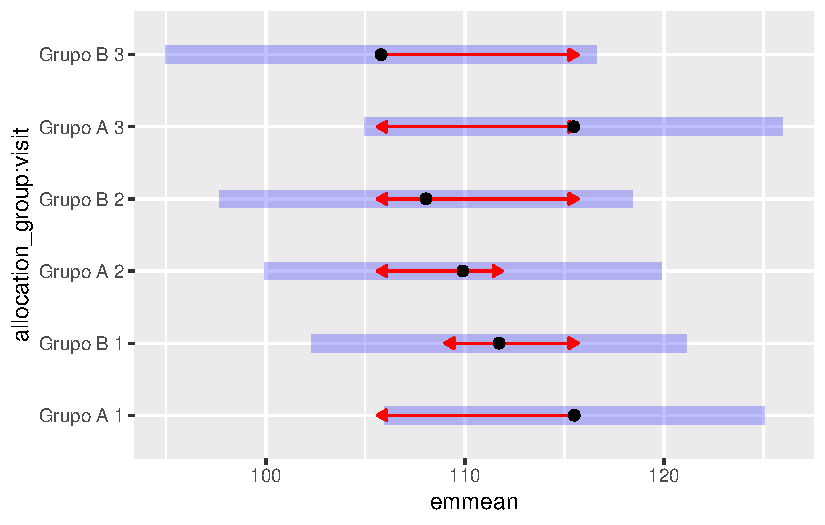
\includegraphics{Outcomes_V1V2V3_files/figure-pdf/labs_ldl_raw_emm-1.pdf}

\begin{Shaded}
\begin{Highlighting}[]
\CommentTok{\# Get EMMs for each group at each visit}
\NormalTok{labs\_ldl\_emm }\OtherTok{\textless{}{-}}\NormalTok{ emmeans}\SpecialCharTok{::}\FunctionTok{emmeans}\NormalTok{(}
\NormalTok{    labs\_ldl\_model\_sens, }
    \SpecialCharTok{\textasciitilde{}}\NormalTok{ allocation\_group }\SpecialCharTok{*}\NormalTok{ visit}
\NormalTok{)}

\NormalTok{labs\_ldl\_emm }\OtherTok{\textless{}{-}} \FunctionTok{regrid}\NormalTok{(labs\_ldl\_emm)}

\CommentTok{\# Table of marginal means}
\NormalTok{labs\_ldl\_emm}
\end{Highlighting}
\end{Shaded}

\begin{verbatim}
 allocation_group visit emmean   SE    df lower.CL upper.CL
 Grupo A          1        114 4.84  80.5    104.1      123
 Grupo B          1        112 4.71  80.5    102.7      121
 Grupo A          2        109 5.00  89.3     99.1      119
 Grupo B          2        109 5.05  99.8     98.7      119
 Grupo A          3        114 5.19 100.3    103.3      124
 Grupo B          3        107 5.21 109.2     96.9      118

Degrees-of-freedom method: inherited from kenward-roger when re-gridding 
Confidence level used: 0.95 
\end{verbatim}

\begin{Shaded}
\begin{Highlighting}[]
\CommentTok{\# Pairwise comparisons: Between groups at each visit}
\NormalTok{emmeans}\SpecialCharTok{::}\FunctionTok{contrast}\NormalTok{(labs\_ldl\_emm, }\AttributeTok{method =} \StringTok{"pairwise"}\NormalTok{, }\AttributeTok{by =} \StringTok{"visit"}\NormalTok{, }\AttributeTok{adjust =} \StringTok{"bonferroni"}\NormalTok{) }\SpecialCharTok{\%\textgreater{}\%} \FunctionTok{summary}\NormalTok{(}\AttributeTok{infer =} \FunctionTok{c}\NormalTok{(}\ConstantTok{TRUE}\NormalTok{, }\ConstantTok{TRUE}\NormalTok{))}
\end{Highlighting}
\end{Shaded}

\begin{verbatim}
visit = 1:
 contrast          estimate   SE    df lower.CL upper.CL t.ratio p.value
 Grupo A - Grupo B    1.661 6.76  80.5   -11.78     15.1   0.246  0.8064

visit = 2:
 contrast          estimate   SE    df lower.CL upper.CL t.ratio p.value
 Grupo A - Grupo B    0.256 7.11  89.3   -13.86     14.4   0.036  0.9713

visit = 3:
 contrast          estimate   SE    df lower.CL upper.CL t.ratio p.value
 Grupo A - Grupo B    6.351 7.35 100.3    -8.24     20.9   0.864  0.3898

Degrees-of-freedom method: inherited from kenward-roger when re-gridding 
Confidence level used: 0.95 
\end{verbatim}

\begin{Shaded}
\begin{Highlighting}[]
\CommentTok{\# Pairwise comparisons: Changes over time within each group}
\NormalTok{emmeans}\SpecialCharTok{::}\FunctionTok{contrast}\NormalTok{(labs\_ldl\_emm, }\AttributeTok{method =} \StringTok{"pairwise"}\NormalTok{, }\AttributeTok{by =} \StringTok{"allocation\_group"}\NormalTok{, }\AttributeTok{adjust =} \StringTok{"bonferroni"}\NormalTok{) }\SpecialCharTok{\%\textgreater{}\%} \FunctionTok{summary}\NormalTok{(}\AttributeTok{infer =} \FunctionTok{c}\NormalTok{(}\ConstantTok{TRUE}\NormalTok{, }\ConstantTok{TRUE}\NormalTok{))}
\end{Highlighting}
\end{Shaded}

\begin{verbatim}
allocation_group = Grupo A:
 contrast        estimate   SE   df lower.CL upper.CL t.ratio p.value
 visit1 - visit2    4.701 3.08 80.5    -2.84    12.24   1.525  0.3936
 visit1 - visit3    0.102 3.38 80.5    -8.16     8.37   0.030  1.0000
 visit2 - visit3   -4.599 3.40 89.3   -12.89     3.69  -1.353  0.5383

allocation_group = Grupo B:
 contrast        estimate   SE   df lower.CL upper.CL t.ratio p.value
 visit1 - visit2    3.297 3.28 80.5    -4.73    11.33   1.004  0.9557
 visit1 - visit3    4.793 3.53 80.5    -3.83    13.42   1.359  0.5339
 visit2 - visit3    1.496 3.67 99.8    -7.44    10.43   0.408  1.0000

Degrees-of-freedom method: inherited from kenward-roger when re-gridding 
Confidence level used: 0.95 
Conf-level adjustment: bonferroni method for 3 estimates 
P value adjustment: bonferroni method for 3 tests 
\end{verbatim}

\begin{Shaded}
\begin{Highlighting}[]
\CommentTok{\# Plot of marginal means}
\FunctionTok{plot}\NormalTok{(labs\_ldl\_emm, }\AttributeTok{comparisons =} \ConstantTok{TRUE}\NormalTok{)}
\end{Highlighting}
\end{Shaded}

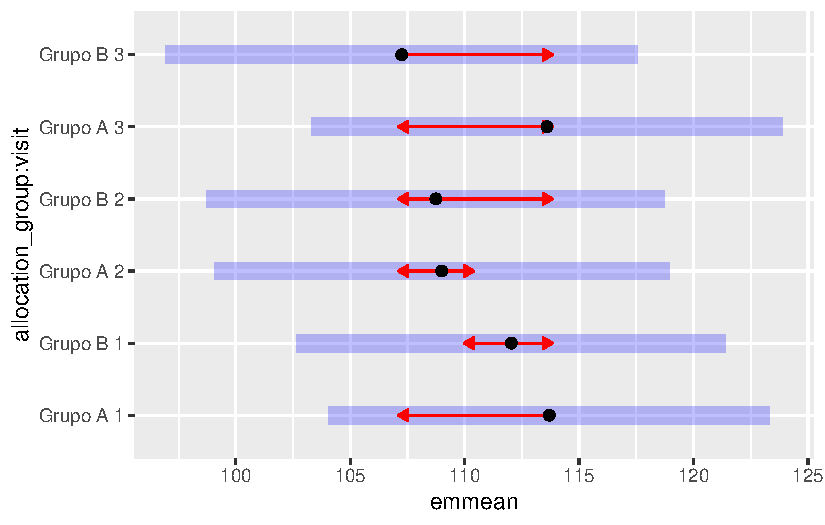
\includegraphics{Outcomes_V1V2V3_files/figure-pdf/labs_ldl_sens_emm-1.pdf}

\begin{Shaded}
\begin{Highlighting}[]
\FunctionTok{ggplot}\NormalTok{(}
    \AttributeTok{data =}\NormalTok{ data\_model, }
    \FunctionTok{aes}\NormalTok{(}
        \AttributeTok{x =} \FunctionTok{as.factor}\NormalTok{(visit),}
        \AttributeTok{y =}\NormalTok{ labs\_ldl,}
        \AttributeTok{group =}\NormalTok{ record\_id,}
\NormalTok{    )}
\NormalTok{) }\SpecialCharTok{+}
    \FunctionTok{geom\_line}\NormalTok{(}\AttributeTok{alpha =} \FloatTok{0.5}\NormalTok{) }\SpecialCharTok{+}
    \FunctionTok{geom\_point}\NormalTok{(}\AttributeTok{alpha =} \FloatTok{0.7}\NormalTok{) }\SpecialCharTok{+}
    \FunctionTok{geom\_smooth}\NormalTok{(}
        \FunctionTok{aes}\NormalTok{(}\AttributeTok{group =}\NormalTok{ allocation\_group),}
        \AttributeTok{method =} \StringTok{"lm"}\NormalTok{,}
        \AttributeTok{se =} \ConstantTok{TRUE}\NormalTok{,}
        \AttributeTok{linewidth =} \DecValTok{1}
\NormalTok{    ) }\SpecialCharTok{+}
    \FunctionTok{labs}\NormalTok{(}\AttributeTok{title =} \StringTok{"All data"}\NormalTok{) }\SpecialCharTok{+}
    \FunctionTok{facet\_wrap}\NormalTok{(}\SpecialCharTok{\textasciitilde{}}\NormalTok{ allocation\_group) }
\end{Highlighting}
\end{Shaded}

\begin{verbatim}
`geom_smooth()` using formula = 'y ~ x'
\end{verbatim}

\begin{verbatim}
Warning: Removed 10 rows containing non-finite outside the scale range
(`stat_smooth()`).
\end{verbatim}

\begin{verbatim}
Warning: Removed 8 rows containing missing values or values outside the scale range
(`geom_line()`).
\end{verbatim}

\begin{verbatim}
Warning: Removed 10 rows containing missing values or values outside the scale range
(`geom_point()`).
\end{verbatim}

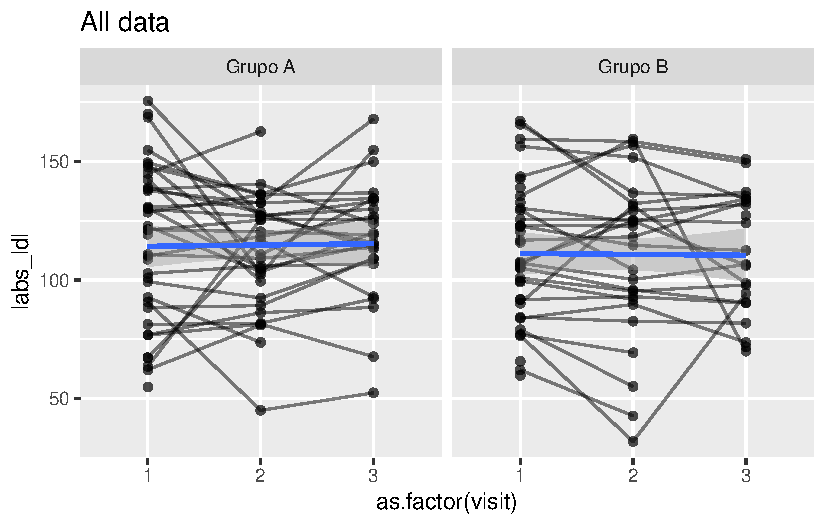
\includegraphics{Outcomes_V1V2V3_files/figure-pdf/labs_ldl_6-1.pdf}

\begin{Shaded}
\begin{Highlighting}[]
    \CommentTok{\#coord\_cartesian(ylim = c(10, 150))}

\NormalTok{data\_model }\SpecialCharTok{\%\textgreater{}\%} 
    \FunctionTok{filter}\NormalTok{(}
        \SpecialCharTok{!}\NormalTok{(record\_id }\SpecialCharTok{\%in\%}\NormalTok{ labs\_ldl\_model\_check}\SpecialCharTok{$}\NormalTok{influential\_ids)}
\NormalTok{    ) }\SpecialCharTok{\%\textgreater{}\%} 
    \FunctionTok{ggplot}\NormalTok{(}
        \FunctionTok{aes}\NormalTok{(}
            \AttributeTok{x =} \FunctionTok{as.factor}\NormalTok{(visit),}
            \AttributeTok{y =}\NormalTok{ labs\_ldl,}
            \AttributeTok{group =}\NormalTok{ record\_id,}
\NormalTok{        )}
\NormalTok{    ) }\SpecialCharTok{+}
    \FunctionTok{geom\_line}\NormalTok{(}\AttributeTok{alpha =} \FloatTok{0.5}\NormalTok{) }\SpecialCharTok{+}
    \FunctionTok{geom\_point}\NormalTok{(}\AttributeTok{alpha =} \FloatTok{0.7}\NormalTok{) }\SpecialCharTok{+}
    \FunctionTok{geom\_smooth}\NormalTok{(}
        \FunctionTok{aes}\NormalTok{(}\AttributeTok{group =}\NormalTok{ allocation\_group),}
        \AttributeTok{method =} \StringTok{"lm"}\NormalTok{,}
        \AttributeTok{se =} \ConstantTok{TRUE}\NormalTok{,}
        \AttributeTok{linewidth =} \DecValTok{1}
\NormalTok{    ) }\SpecialCharTok{+}
    \FunctionTok{labs}\NormalTok{(}\AttributeTok{title =} \StringTok{"Sensitivity analysis"}\NormalTok{) }\SpecialCharTok{+}
    \FunctionTok{facet\_wrap}\NormalTok{(}\SpecialCharTok{\textasciitilde{}}\NormalTok{ allocation\_group) }
\end{Highlighting}
\end{Shaded}

\begin{verbatim}
`geom_smooth()` using formula = 'y ~ x'
\end{verbatim}

\begin{verbatim}
Warning: Removed 10 rows containing non-finite outside the scale range
(`stat_smooth()`).
\end{verbatim}

\begin{verbatim}
Warning: Removed 8 rows containing missing values or values outside the scale range
(`geom_line()`).
\end{verbatim}

\begin{verbatim}
Warning: Removed 10 rows containing missing values or values outside the scale range
(`geom_point()`).
\end{verbatim}

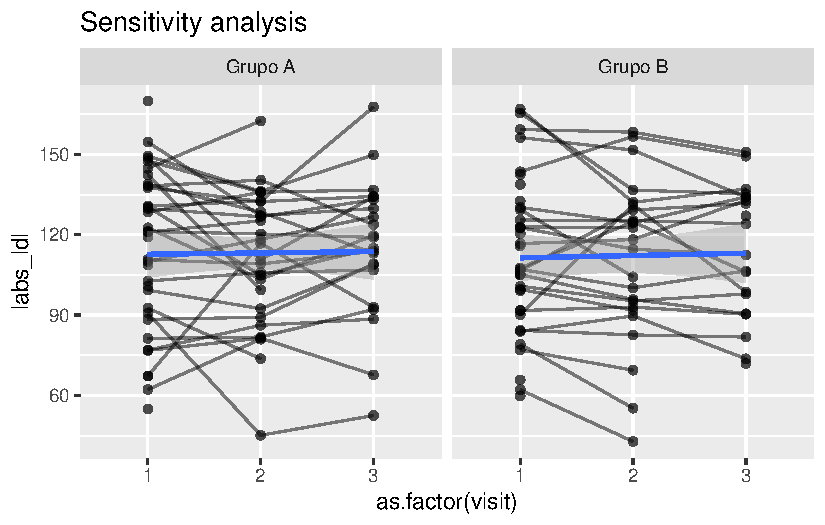
\includegraphics{Outcomes_V1V2V3_files/figure-pdf/labs_ldl_6-2.pdf}

\begin{Shaded}
\begin{Highlighting}[]
    \CommentTok{\#coord\_cartesian(ylim = c(10, 150))}
\end{Highlighting}
\end{Shaded}

\subsubsection{HDL Colesterol}\label{hdl-colesterol}

Variável: \texttt{labs\_hdl}

\begin{Shaded}
\begin{Highlighting}[]
\CommentTok{\# Plot 1: Raw data}
\NormalTok{labs\_hdl\_hist\_1 }\OtherTok{\textless{}{-}}\NormalTok{ data\_model }\SpecialCharTok{\%\textgreater{}\%} 
    \CommentTok{\#filter(}
    \CommentTok{\#    labs\_hdl \textless{} 300}
    \CommentTok{\#) \%\textgreater{}\% }
    \FunctionTok{ggplot}\NormalTok{(}\FunctionTok{aes}\NormalTok{(}\AttributeTok{x =}\NormalTok{ labs\_hdl)) }\SpecialCharTok{+} 
    \FunctionTok{geom\_histogram}\NormalTok{(}\AttributeTok{bins =} \DecValTok{50}\NormalTok{, }\AttributeTok{fill =} \StringTok{"skyblue"}\NormalTok{, }\AttributeTok{color =} \StringTok{"black"}\NormalTok{)}

\CommentTok{\# Plot 2: Log{-}transformed data}
\NormalTok{labs\_hdl\_hist\_2 }\OtherTok{\textless{}{-}}\NormalTok{ data\_model }\SpecialCharTok{\%\textgreater{}\%} 
    \CommentTok{\#filter(}
    \CommentTok{\#    labs\_hdl \textless{} 300}
    \CommentTok{\#) \%\textgreater{}\%}
    \FunctionTok{ggplot}\NormalTok{(}\FunctionTok{aes}\NormalTok{(}\AttributeTok{x =} \FunctionTok{log1p}\NormalTok{(labs\_hdl))) }\SpecialCharTok{+} 
    \FunctionTok{geom\_histogram}\NormalTok{(}\AttributeTok{bins =} \DecValTok{50}\NormalTok{, }\AttributeTok{fill =} \StringTok{"lightgreen"}\NormalTok{, }\AttributeTok{color =} \StringTok{"black"}\NormalTok{)}

\CommentTok{\# Combine side by side}
\NormalTok{labs\_hdl\_hist\_1 }\SpecialCharTok{+}\NormalTok{ labs\_hdl\_hist\_2 }\CommentTok{\# library(patchwork)}
\end{Highlighting}
\end{Shaded}

\begin{verbatim}
Warning: Removed 10 rows containing non-finite outside the scale range (`stat_bin()`).
Removed 10 rows containing non-finite outside the scale range (`stat_bin()`).
\end{verbatim}

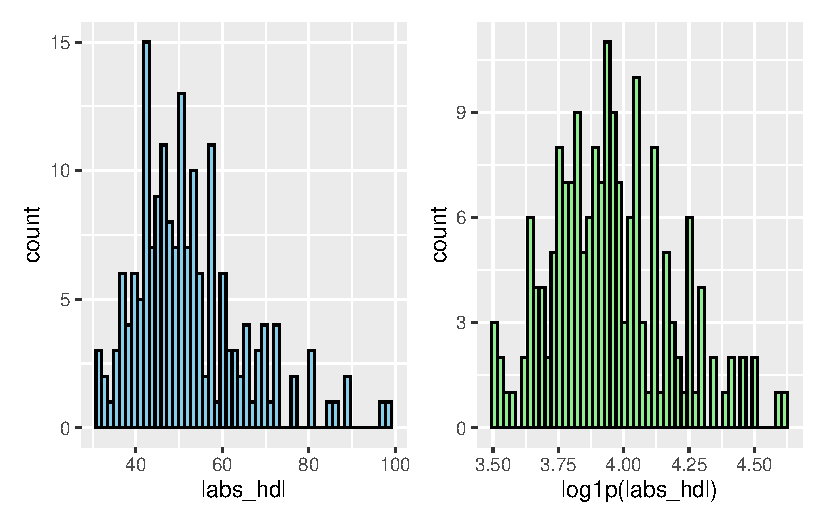
\includegraphics{Outcomes_V1V2V3_files/figure-pdf/labs_hdl_1-1.pdf}

\begin{Shaded}
\begin{Highlighting}[]
\CommentTok{\# LMM}
\NormalTok{labs\_hdl\_model }\OtherTok{\textless{}{-}} \FunctionTok{lmer}\NormalTok{(}\FunctionTok{log1p}\NormalTok{(labs\_hdl) }\SpecialCharTok{\textasciitilde{}}\NormalTok{ allocation\_group }\SpecialCharTok{*}\NormalTok{ visit }\SpecialCharTok{+}\NormalTok{ (}\DecValTok{1} \SpecialCharTok{|}\NormalTok{ record\_id), }\AttributeTok{data =}\NormalTok{ data\_model)}
\FunctionTok{check\_collinearity}\NormalTok{(labs\_hdl\_model)}
\end{Highlighting}
\end{Shaded}

\begin{verbatim}
# Check for Multicollinearity

Low Correlation

                   Term  VIF   VIF 95% CI Increased SE Tolerance
       allocation_group 1.16 [1.05, 1.51]         1.08      0.86
                  visit 3.49 [2.78, 4.48]         1.87      0.29
 allocation_group:visit 3.74 [2.97, 4.81]         1.93      0.27
 Tolerance 95% CI
     [0.66, 0.95]
     [0.22, 0.36]
     [0.21, 0.34]
\end{verbatim}

\begin{Shaded}
\begin{Highlighting}[]
\CommentTok{\# Sensitivity analysis}
\NormalTok{labs\_hdl\_model\_check }\OtherTok{\textless{}{-}} \FunctionTok{sensitivity\_check\_lmer}\NormalTok{(}
    \AttributeTok{model =}\NormalTok{ labs\_hdl\_model,}
    \AttributeTok{id\_var =} \StringTok{"record\_id"}\NormalTok{,}
    \AttributeTok{top\_n =} \DecValTok{5}\NormalTok{)}

\CommentTok{\# LMM Sensitivity}
\NormalTok{labs\_hdl\_model\_sens }\OtherTok{\textless{}{-}} \FunctionTok{update}\NormalTok{(}\AttributeTok{object =}\NormalTok{ labs\_hdl\_model,}
                              \AttributeTok{subset =} \SpecialCharTok{!}\NormalTok{(record\_id }\SpecialCharTok{\%in\%}\NormalTok{ labs\_hdl\_model\_check}\SpecialCharTok{$}\NormalTok{influential\_ids))}
\CommentTok{\# Influential IDS}
\NormalTok{labs\_hdl\_model\_check}\SpecialCharTok{$}\NormalTok{influential\_ids}
\end{Highlighting}
\end{Shaded}

\begin{verbatim}
[1] "16" "75" "38" "42" "26"
\end{verbatim}

\paragraph{Resumo dos modelos}\label{resumo-dos-modelos-6}

\begin{Shaded}
\begin{Highlighting}[]
\CommentTok{\# Model comparison}
\FunctionTok{summary}\NormalTok{(labs\_hdl\_model)}
\end{Highlighting}
\end{Shaded}

\begin{verbatim}
Linear mixed model fit by REML. t-tests use Satterthwaite's method [
lmerModLmerTest]
Formula: log1p(labs_hdl) ~ allocation_group * visit + (1 | record_id)
   Data: data_model

REML criterion at convergence: -79.8

Scaled residuals: 
    Min      1Q  Median      3Q     Max 
-2.4161 -0.4907 -0.0289  0.4389  3.0395 

Random effects:
 Groups    Name        Variance Std.Dev.
 record_id (Intercept) 0.03949  0.1987  
 Residual              0.01437  0.1199  
Number of obs: 179, groups:  record_id, 75

Fixed effects:
                                Estimate Std. Error        df t value Pr(>|t|)
(Intercept)                      3.94481    0.03815  94.81644 103.399   <2e-16
allocation_groupGrupo B          0.06500    0.05360  94.81644   1.213    0.228
visit2                          -0.01725    0.03011 102.74671  -0.573    0.568
visit3                          -0.01928    0.03264 103.82312  -0.591    0.556
allocation_groupGrupo B:visit2  -0.02214    0.04420 104.26672  -0.501    0.618
allocation_groupGrupo B:visit3  -0.03185    0.04749 105.05887  -0.671    0.504
                                  
(Intercept)                    ***
allocation_groupGrupo B           
visit2                            
visit3                            
allocation_groupGrupo B:visit2    
allocation_groupGrupo B:visit3    
---
Signif. codes:  0 '***' 0.001 '**' 0.01 '*' 0.05 '.' 0.1 ' ' 1

Correlation of Fixed Effects:
            (Intr) all_GB visit2 visit3 a_GB:2
allctn_grGB -0.712                            
visit2      -0.338  0.241                     
visit3      -0.312  0.222  0.451              
allctn_GB:2  0.230 -0.324 -0.681 -0.307       
allctn_GB:3  0.214 -0.301 -0.310 -0.687  0.435
\end{verbatim}

\begin{Shaded}
\begin{Highlighting}[]
\FunctionTok{summary}\NormalTok{(labs\_hdl\_model\_sens)}
\end{Highlighting}
\end{Shaded}

\begin{verbatim}
Linear mixed model fit by REML. t-tests use Satterthwaite's method [
lmerModLmerTest]
Formula: log1p(labs_hdl) ~ allocation_group * visit + (1 | record_id)
   Data: data_model
 Subset: !(record_id %in% labs_hdl_model_check$influential_ids)

REML criterion at convergence: -109.5

Scaled residuals: 
     Min       1Q   Median       3Q      Max 
-1.93721 -0.52772 -0.00876  0.50466  2.04629 

Random effects:
 Groups    Name        Variance Std.Dev.
 record_id (Intercept) 0.03870  0.1967  
 Residual              0.01007  0.1004  
Number of obs: 166, groups:  record_id, 70

Fixed effects:
                               Estimate Std. Error       df t value Pr(>|t|)
(Intercept)                     3.92823    0.03733 82.44138 105.230   <2e-16
allocation_groupGrupo B         0.06708    0.05279 82.44138   1.271    0.207
visit2                         -0.01029    0.02612 93.87428  -0.394    0.695
visit3                         -0.01338    0.02805 94.47459  -0.477    0.635
allocation_groupGrupo B:visit2 -0.02943    0.03859 95.06373  -0.763    0.448
allocation_groupGrupo B:visit3 -0.03861    0.04187 95.58326  -0.922    0.359
                                  
(Intercept)                    ***
allocation_groupGrupo B           
visit2                            
visit3                            
allocation_groupGrupo B:visit2    
allocation_groupGrupo B:visit3    
---
Signif. codes:  0 '***' 0.001 '**' 0.01 '*' 0.05 '.' 0.1 ' ' 1

Correlation of Fixed Effects:
            (Intr) all_GB visit2 visit3 a_GB:2
allctn_grGB -0.707                            
visit2      -0.295  0.209                     
visit3      -0.275  0.194  0.457              
allctn_GB:2  0.200 -0.283 -0.677 -0.310       
allctn_GB:3  0.184 -0.260 -0.306 -0.670  0.440
\end{verbatim}

\begin{Shaded}
\begin{Highlighting}[]
\NormalTok{labs\_hdl\_model\_check}\SpecialCharTok{$}\NormalTok{comparison\_table}
\end{Highlighting}
\end{Shaded}

\begin{verbatim}
# A tibble: 16 x 6
   Model       term                       estimate std.error statistic   p.value
   <chr>       <chr>                         <dbl>     <dbl>     <dbl>     <dbl>
 1 Original    (Intercept)                  3.94      0.0382   103.     2.78e-99
 2 Sensitivity (Intercept)                  3.93      0.0373   105.     1.23e-89
 3 Original    allocation_groupGrupo B      0.0650    0.0536     1.21   2.28e- 1
 4 Sensitivity allocation_groupGrupo B      0.0671    0.0528     1.27   2.07e- 1
 5 Original    allocation_groupGrupo B:v~  -0.0221    0.0442    -0.501  6.18e- 1
 6 Sensitivity allocation_groupGrupo B:v~  -0.0294    0.0386    -0.763  4.48e- 1
 7 Original    allocation_groupGrupo B:v~  -0.0318    0.0475    -0.671  5.04e- 1
 8 Sensitivity allocation_groupGrupo B:v~  -0.0386    0.0419    -0.922  3.59e- 1
 9 Original    sd__(Intercept)              0.199    NA         NA     NA       
10 Sensitivity sd__(Intercept)              0.197    NA         NA     NA       
11 Original    sd__Observation              0.120    NA         NA     NA       
12 Sensitivity sd__Observation              0.100    NA         NA     NA       
13 Original    visit2                      -0.0172    0.0301    -0.573  5.68e- 1
14 Sensitivity visit2                      -0.0103    0.0261    -0.394  6.95e- 1
15 Original    visit3                      -0.0193    0.0326    -0.591  5.56e- 1
16 Sensitivity visit3                      -0.0134    0.0281    -0.477  6.35e- 1
\end{verbatim}

\begin{Shaded}
\begin{Highlighting}[]
\NormalTok{performance}\SpecialCharTok{::}\FunctionTok{compare\_performance}\NormalTok{(labs\_hdl\_model, labs\_hdl\_model\_sens)}
\end{Highlighting}
\end{Shaded}

\begin{verbatim}
When comparing models, please note that probably not all models were fit
  from same data.
\end{verbatim}

\begin{verbatim}
# Comparison of Model Performance Indices

Name                |           Model |  AIC (weights) | AICc (weights)
-----------------------------------------------------------------------
labs_hdl_model      | lmerModLmerTest | 1319.8 (<.001) | 1320.7 (<.001)
labs_hdl_model_sens | lmerModLmerTest | 1181.6 (>.999) | 1182.5 (>.999)

Name                |  BIC (weights) | R2 (cond.) | R2 (marg.) |   ICC |  RMSE | Sigma
--------------------------------------------------------------------------------------
labs_hdl_model      | 1345.3 (<.001) |      0.738 |      0.017 | 0.733 | 0.094 | 0.120
labs_hdl_model_sens | 1206.5 (>.999) |      0.797 |      0.018 | 0.793 | 0.078 | 0.100
\end{verbatim}

\begin{Shaded}
\begin{Highlighting}[]
\NormalTok{performance}\SpecialCharTok{::}\FunctionTok{check\_model}\NormalTok{(labs\_hdl\_model)}
\end{Highlighting}
\end{Shaded}

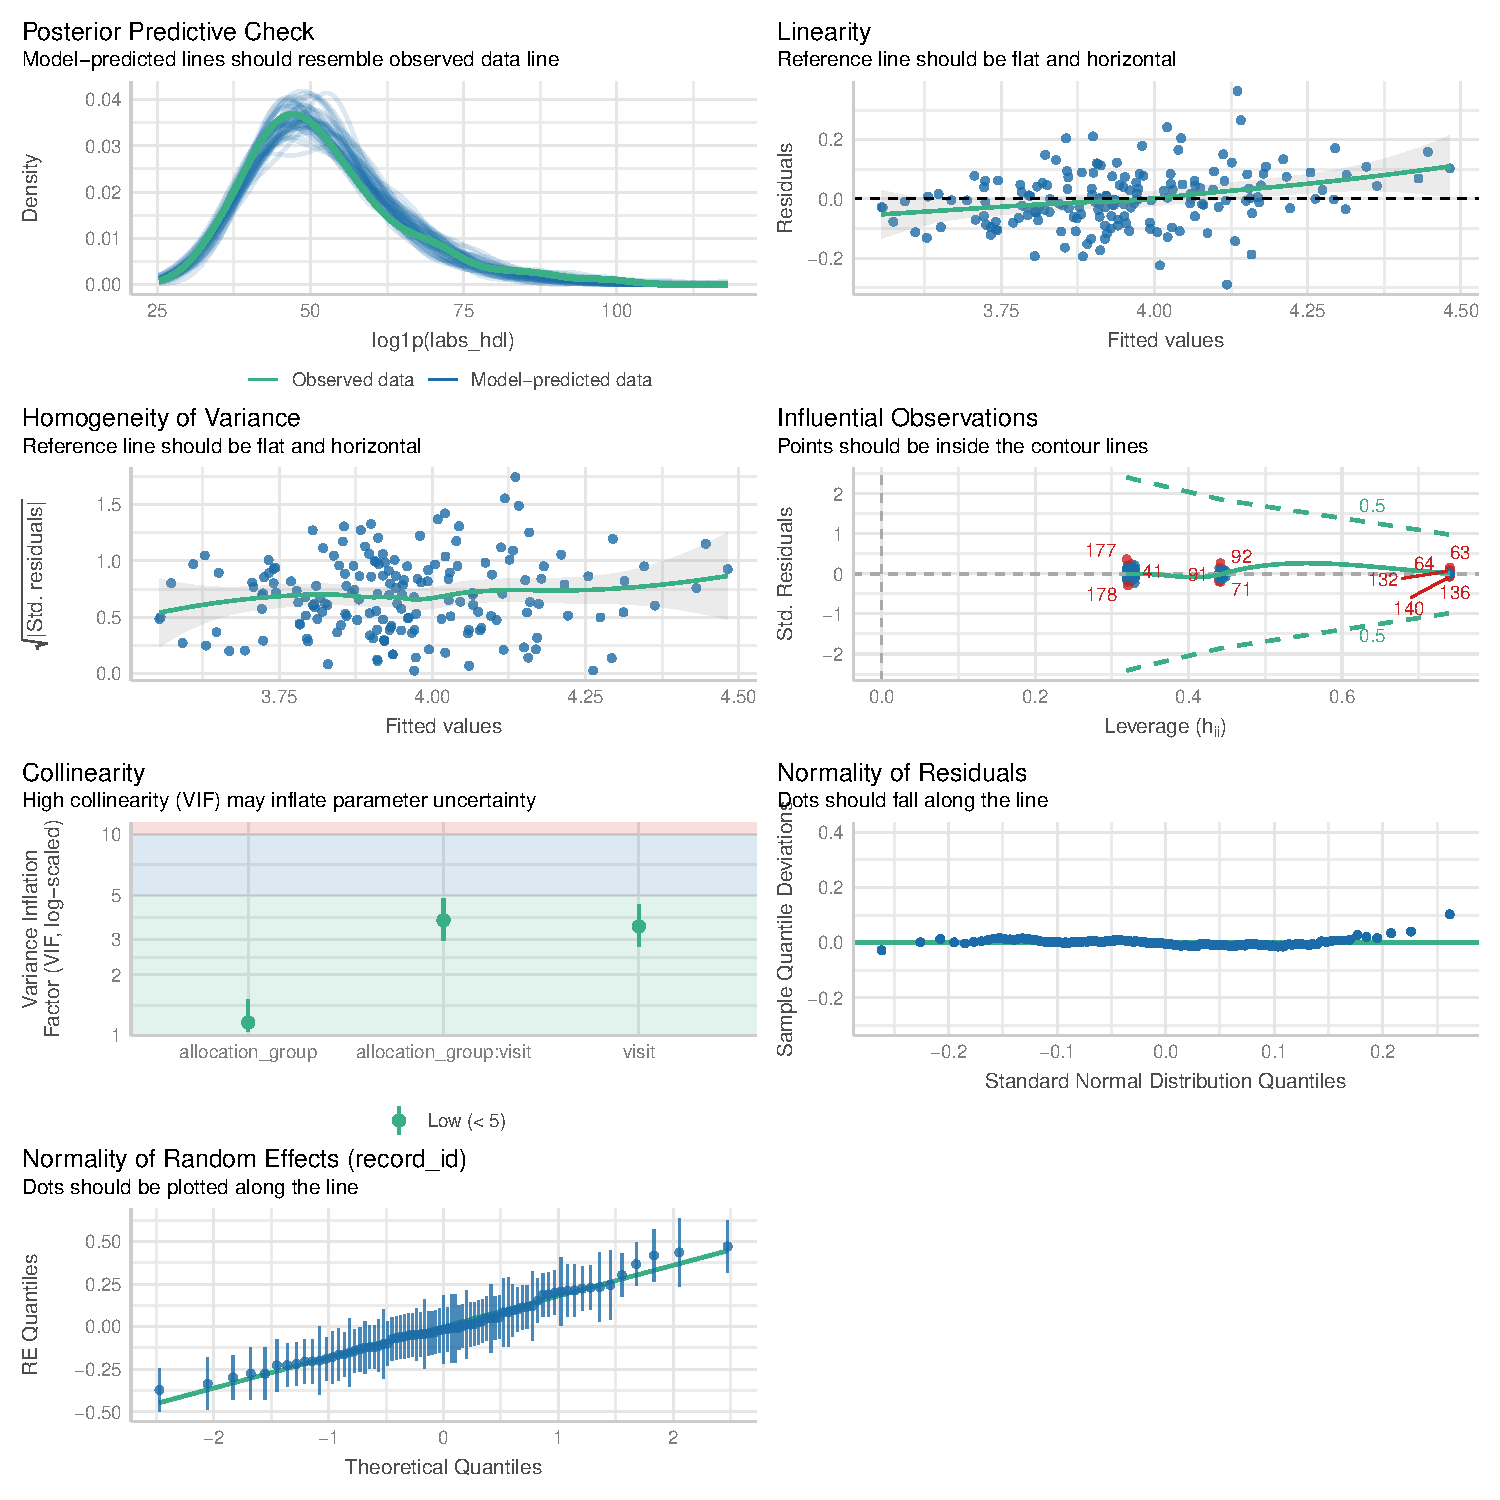
\includegraphics{Outcomes_V1V2V3_files/figure-pdf/labs_hdl_4-1.pdf}

\begin{Shaded}
\begin{Highlighting}[]
\NormalTok{performance}\SpecialCharTok{::}\FunctionTok{check\_model}\NormalTok{(labs\_hdl\_model\_sens)}
\end{Highlighting}
\end{Shaded}

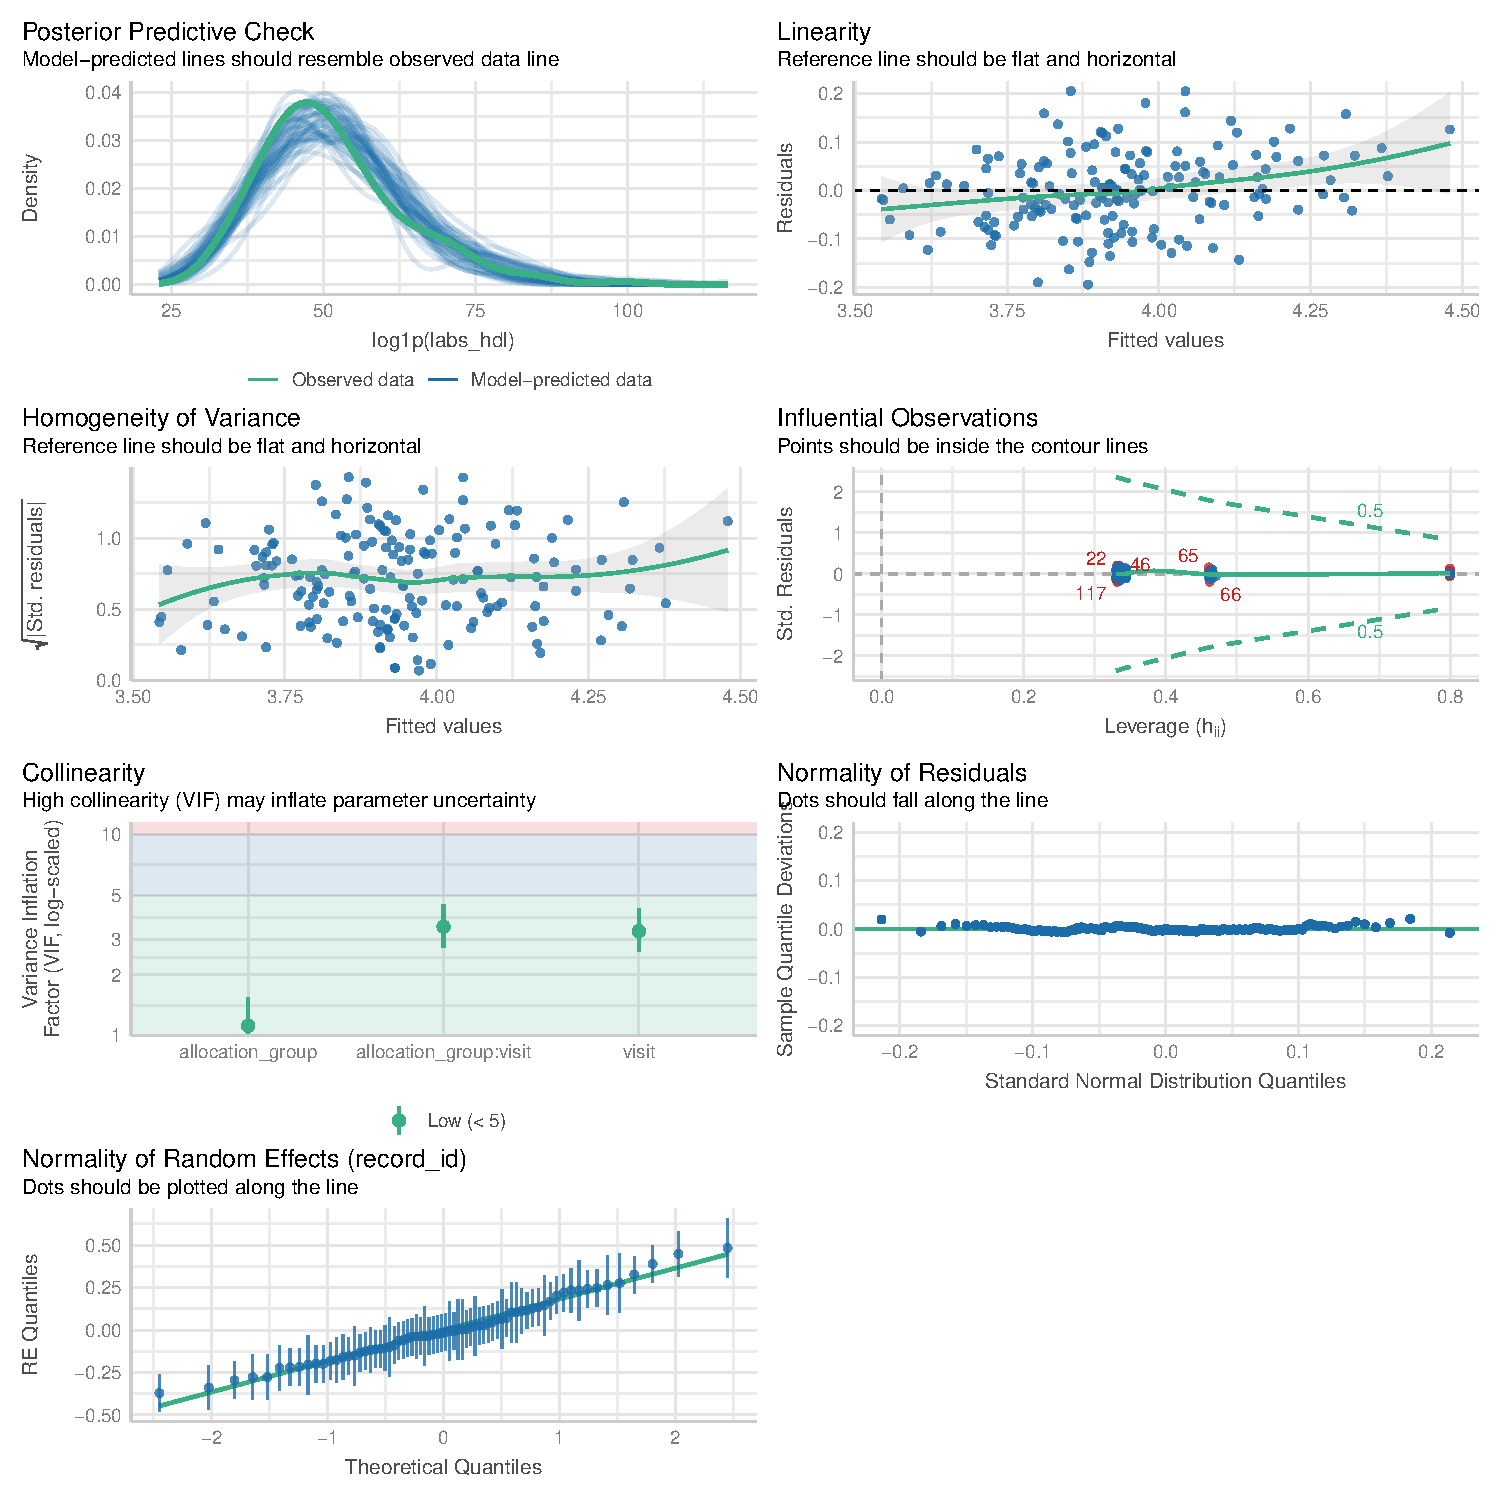
\includegraphics{Outcomes_V1V2V3_files/figure-pdf/labs_hdl_4-2.pdf}

\paragraph{Médias Marginais
Estimadas}\label{muxe9dias-marginais-estimadas-6}

\begin{Shaded}
\begin{Highlighting}[]
\CommentTok{\# Get EMMs for each group at each visit}
\NormalTok{labs\_hdl\_raw\_emm }\OtherTok{\textless{}{-}}\NormalTok{ emmeans}\SpecialCharTok{::}\FunctionTok{emmeans}\NormalTok{(}
\NormalTok{    labs\_hdl\_model, }
    \SpecialCharTok{\textasciitilde{}}\NormalTok{ allocation\_group }\SpecialCharTok{*}\NormalTok{ visit}
\NormalTok{)}

\NormalTok{labs\_hdl\_raw\_emm }\OtherTok{\textless{}{-}} \FunctionTok{regrid}\NormalTok{(labs\_hdl\_raw\_emm)}

\CommentTok{\# Table of marginal means}
\NormalTok{labs\_hdl\_raw\_emm}
\end{Highlighting}
\end{Shaded}

\begin{verbatim}
 allocation_group visit response   SE    df lower.CL upper.CL
 Grupo A          1         50.7 1.97  96.4     46.8     54.6
 Grupo B          1         54.1 2.08  96.4     50.0     58.3
 Grupo A          2         49.8 2.02 108.6     45.8     53.8
 Grupo B          2         52.0 2.19 123.2     47.7     56.3
 Grupo A          3         49.7 2.12 123.5     45.5     53.9
 Grupo B          3         51.4 2.26 135.2     46.9     55.9

Degrees-of-freedom method: inherited from kenward-roger when re-gridding 
Confidence level used: 0.95 
\end{verbatim}

\begin{Shaded}
\begin{Highlighting}[]
\CommentTok{\# Pairwise comparisons: Between groups at each visit}
\NormalTok{emmeans}\SpecialCharTok{::}\FunctionTok{contrast}\NormalTok{(labs\_hdl\_raw\_emm, }\AttributeTok{method =} \StringTok{"pairwise"}\NormalTok{, }\AttributeTok{by =} \StringTok{"visit"}\NormalTok{, }\AttributeTok{adjust =} \StringTok{"bonferroni"}\NormalTok{) }\SpecialCharTok{\%\textgreater{}\%} \FunctionTok{summary}\NormalTok{(}\AttributeTok{infer =} \FunctionTok{c}\NormalTok{(}\ConstantTok{TRUE}\NormalTok{, }\ConstantTok{TRUE}\NormalTok{))}
\end{Highlighting}
\end{Shaded}

\begin{verbatim}
visit = 1:
 contrast          estimate   SE    df lower.CL upper.CL t.ratio p.value
 Grupo A - Grupo B    -3.47 2.86  96.4    -9.15     2.21  -1.212  0.2284

visit = 2:
 contrast          estimate   SE    df lower.CL upper.CL t.ratio p.value
 Grupo A - Grupo B    -2.22 2.98 108.6    -8.14     3.69  -0.746  0.4576

visit = 3:
 contrast          estimate   SE    df lower.CL upper.CL t.ratio p.value
 Grupo A - Grupo B    -1.71 3.09 123.5    -7.83     4.42  -0.552  0.5819

Degrees-of-freedom method: inherited from kenward-roger when re-gridding 
Confidence level used: 0.95 
\end{verbatim}

\begin{Shaded}
\begin{Highlighting}[]
\CommentTok{\# Pairwise comparisons: Changes over time within each group}
\NormalTok{emmeans}\SpecialCharTok{::}\FunctionTok{contrast}\NormalTok{(labs\_hdl\_raw\_emm, }\AttributeTok{method =} \StringTok{"pairwise"}\NormalTok{, }\AttributeTok{by =} \StringTok{"allocation\_group"}\NormalTok{, }\AttributeTok{adjust =} \StringTok{"bonferroni"}\NormalTok{) }\SpecialCharTok{\%\textgreater{}\%} \FunctionTok{summary}\NormalTok{(}\AttributeTok{infer =} \FunctionTok{c}\NormalTok{(}\ConstantTok{TRUE}\NormalTok{, }\ConstantTok{TRUE}\NormalTok{))}
\end{Highlighting}
\end{Shaded}

\begin{verbatim}
allocation_group = Grupo A:
 contrast        estimate   SE    df lower.CL upper.CL t.ratio p.value
 visit1 - visit2    0.883 1.54  96.4    -2.87     4.64   0.573  1.0000
 visit1 - visit3    0.986 1.67  96.4    -3.08     5.05   0.591  1.0000
 visit2 - visit3    0.103 1.67 108.6    -3.96     4.17   0.062  1.0000

allocation_group = Grupo B:
 contrast        estimate   SE    df lower.CL upper.CL t.ratio p.value
 visit1 - visit2    2.129 1.74  96.4    -2.12     6.38   1.221  0.6751
 visit1 - visit3    2.748 1.84  96.4    -1.74     7.24   1.491  0.4175
 visit2 - visit3    0.619 1.90 123.2    -3.99     5.22   0.326  1.0000

Degrees-of-freedom method: inherited from kenward-roger when re-gridding 
Confidence level used: 0.95 
Conf-level adjustment: bonferroni method for 3 estimates 
P value adjustment: bonferroni method for 3 tests 
\end{verbatim}

\begin{Shaded}
\begin{Highlighting}[]
\CommentTok{\# Plot of marginal means}
\FunctionTok{plot}\NormalTok{(labs\_hdl\_raw\_emm, }\AttributeTok{comparisons =} \ConstantTok{TRUE}\NormalTok{)}
\end{Highlighting}
\end{Shaded}

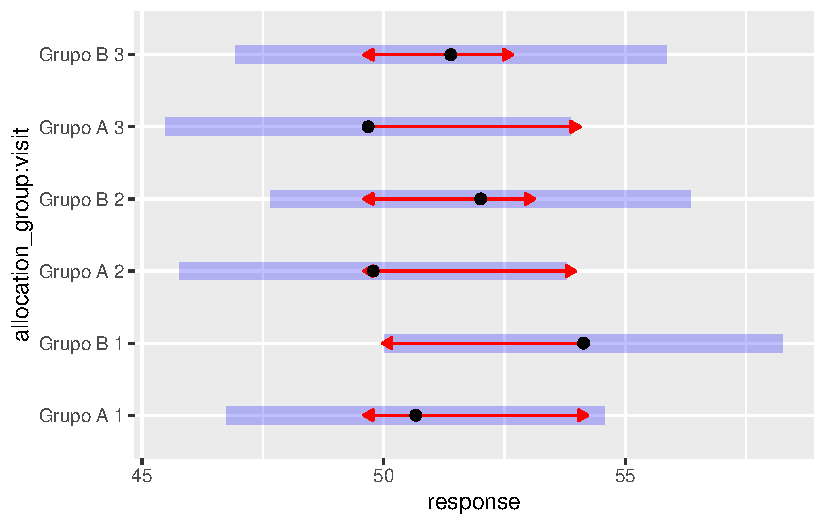
\includegraphics{Outcomes_V1V2V3_files/figure-pdf/labs_hdl_raw_emm-1.pdf}

\begin{Shaded}
\begin{Highlighting}[]
\CommentTok{\# Get EMMs for each group at each visit}
\NormalTok{labs\_hdl\_emm }\OtherTok{\textless{}{-}}\NormalTok{ emmeans}\SpecialCharTok{::}\FunctionTok{emmeans}\NormalTok{(}
\NormalTok{    labs\_hdl\_model\_sens, }
    \SpecialCharTok{\textasciitilde{}}\NormalTok{ allocation\_group }\SpecialCharTok{*}\NormalTok{ visit}
\NormalTok{)}

\NormalTok{labs\_hdl\_emm }\OtherTok{\textless{}{-}} \FunctionTok{regrid}\NormalTok{(labs\_hdl\_emm)}

\CommentTok{\# Table of marginal means}
\NormalTok{labs\_hdl\_emm}
\end{Highlighting}
\end{Shaded}

\begin{verbatim}
 allocation_group visit response   SE    df lower.CL upper.CL
 Grupo A          1         49.8 1.90  83.9     46.0     53.6
 Grupo B          1         53.3 2.03  83.9     49.3     57.4
 Grupo A          2         49.3 1.95  93.9     45.4     53.2
 Grupo B          2         51.2 2.11 105.0     47.1     55.4
 Grupo A          3         49.1 2.01 104.0     45.2     53.1
 Grupo B          3         50.6 2.18 118.8     46.3     54.9

Degrees-of-freedom method: inherited from kenward-roger when re-gridding 
Confidence level used: 0.95 
\end{verbatim}

\begin{Shaded}
\begin{Highlighting}[]
\CommentTok{\# Pairwise comparisons: Between groups at each visit}
\NormalTok{emmeans}\SpecialCharTok{::}\FunctionTok{contrast}\NormalTok{(labs\_hdl\_emm, }\AttributeTok{method =} \StringTok{"pairwise"}\NormalTok{, }\AttributeTok{by =} \StringTok{"visit"}\NormalTok{, }\AttributeTok{adjust =} \StringTok{"bonferroni"}\NormalTok{) }\SpecialCharTok{\%\textgreater{}\%} \FunctionTok{summary}\NormalTok{(}\AttributeTok{infer =} \FunctionTok{c}\NormalTok{(}\ConstantTok{TRUE}\NormalTok{, }\ConstantTok{TRUE}\NormalTok{))}
\end{Highlighting}
\end{Shaded}

\begin{verbatim}
visit = 1:
 contrast          estimate   SE    df lower.CL upper.CL t.ratio p.value
 Grupo A - Grupo B    -3.53 2.78  83.9    -9.05     2.00  -1.269  0.2078

visit = 2:
 contrast          estimate   SE    df lower.CL upper.CL t.ratio p.value
 Grupo A - Grupo B    -1.93 2.87  93.9    -7.63     3.77  -0.672  0.5029

visit = 3:
 contrast          estimate   SE    df lower.CL upper.CL t.ratio p.value
 Grupo A - Grupo B    -1.45 2.97 104.0    -7.33     4.43  -0.488  0.6264

Degrees-of-freedom method: inherited from kenward-roger when re-gridding 
Confidence level used: 0.95 
\end{verbatim}

\begin{Shaded}
\begin{Highlighting}[]
\CommentTok{\# Pairwise comparisons: Changes over time within each group}
\NormalTok{emmeans}\SpecialCharTok{::}\FunctionTok{contrast}\NormalTok{(labs\_hdl\_emm, }\AttributeTok{method =} \StringTok{"pairwise"}\NormalTok{, }\AttributeTok{by =} \StringTok{"allocation\_group"}\NormalTok{, }\AttributeTok{adjust =} \StringTok{"bonferroni"}\NormalTok{) }\SpecialCharTok{\%\textgreater{}\%} \FunctionTok{summary}\NormalTok{(}\AttributeTok{infer =} \FunctionTok{c}\NormalTok{(}\ConstantTok{TRUE}\NormalTok{, }\ConstantTok{TRUE}\NormalTok{))}
\end{Highlighting}
\end{Shaded}

\begin{verbatim}
allocation_group = Grupo A:
 contrast        estimate   SE    df lower.CL upper.CL t.ratio p.value
 visit1 - visit2    0.520 1.32  83.9    -2.71     3.75   0.394  1.0000
 visit1 - visit3    0.675 1.41  83.9    -2.78     4.13   0.477  1.0000
 visit2 - visit3    0.155 1.42  93.9    -3.31     3.62   0.109  1.0000

allocation_group = Grupo B:
 contrast        estimate   SE    df lower.CL upper.CL t.ratio p.value
 visit1 - visit2    2.116 1.51  83.9    -1.57     5.80   1.403  0.4931
 visit1 - visit3    2.753 1.63  83.9    -1.24     6.75   1.684  0.2874
 visit2 - visit3    0.637 1.66 105.0    -3.40     4.67   0.384  1.0000

Degrees-of-freedom method: inherited from kenward-roger when re-gridding 
Confidence level used: 0.95 
Conf-level adjustment: bonferroni method for 3 estimates 
P value adjustment: bonferroni method for 3 tests 
\end{verbatim}

\begin{Shaded}
\begin{Highlighting}[]
\CommentTok{\# Plot of marginal means}
\FunctionTok{plot}\NormalTok{(labs\_hdl\_emm, }\AttributeTok{comparisons =} \ConstantTok{TRUE}\NormalTok{)}
\end{Highlighting}
\end{Shaded}

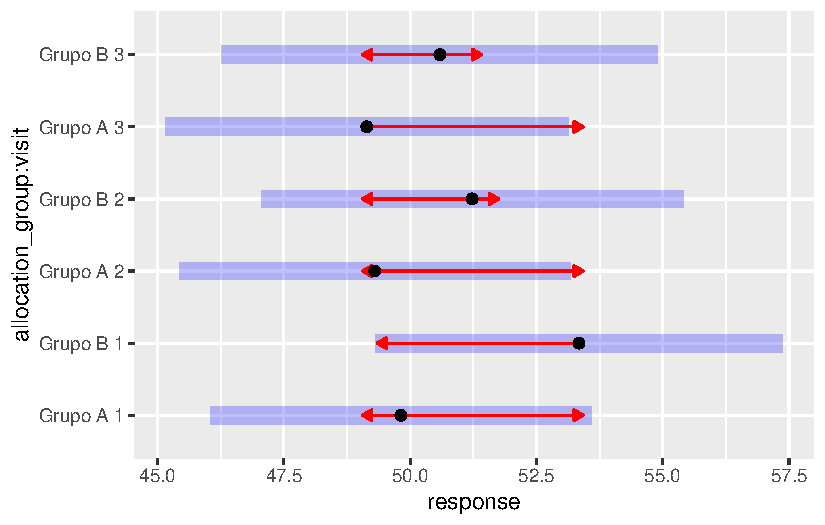
\includegraphics{Outcomes_V1V2V3_files/figure-pdf/labs_hdl_sens_emm-1.pdf}

\begin{Shaded}
\begin{Highlighting}[]
\FunctionTok{ggplot}\NormalTok{(}
    \AttributeTok{data =}\NormalTok{ data\_model, }
    \FunctionTok{aes}\NormalTok{(}
        \AttributeTok{x =} \FunctionTok{as.factor}\NormalTok{(visit),}
        \AttributeTok{y =}\NormalTok{ labs\_hdl,}
        \AttributeTok{group =}\NormalTok{ record\_id,}
\NormalTok{    )}
\NormalTok{) }\SpecialCharTok{+}
    \FunctionTok{geom\_line}\NormalTok{(}\AttributeTok{alpha =} \FloatTok{0.5}\NormalTok{) }\SpecialCharTok{+}
    \FunctionTok{geom\_point}\NormalTok{(}\AttributeTok{alpha =} \FloatTok{0.7}\NormalTok{) }\SpecialCharTok{+}
    \FunctionTok{geom\_smooth}\NormalTok{(}
        \FunctionTok{aes}\NormalTok{(}\AttributeTok{group =}\NormalTok{ allocation\_group),}
        \AttributeTok{method =} \StringTok{"lm"}\NormalTok{,}
        \AttributeTok{se =} \ConstantTok{TRUE}\NormalTok{,}
        \AttributeTok{linewidth =} \DecValTok{1}
\NormalTok{    ) }\SpecialCharTok{+}
    \FunctionTok{labs}\NormalTok{(}\AttributeTok{title =} \StringTok{"All data"}\NormalTok{) }\SpecialCharTok{+}
    \FunctionTok{facet\_wrap}\NormalTok{(}\SpecialCharTok{\textasciitilde{}}\NormalTok{ allocation\_group) }
\end{Highlighting}
\end{Shaded}

\begin{verbatim}
`geom_smooth()` using formula = 'y ~ x'
\end{verbatim}

\begin{verbatim}
Warning: Removed 10 rows containing non-finite outside the scale range
(`stat_smooth()`).
\end{verbatim}

\begin{verbatim}
Warning: Removed 8 rows containing missing values or values outside the scale range
(`geom_line()`).
\end{verbatim}

\begin{verbatim}
Warning: Removed 10 rows containing missing values or values outside the scale range
(`geom_point()`).
\end{verbatim}

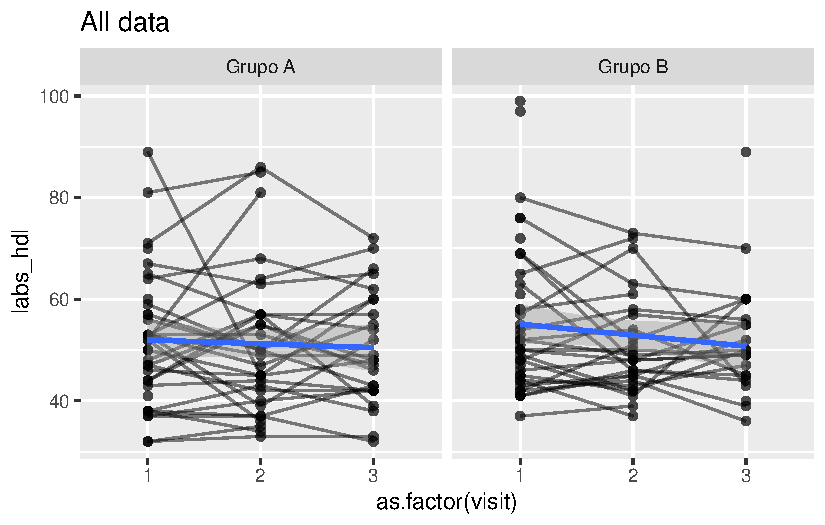
\includegraphics{Outcomes_V1V2V3_files/figure-pdf/labs_hdl_6-1.pdf}

\begin{Shaded}
\begin{Highlighting}[]
    \CommentTok{\#coord\_cartesian(ylim = c(10, 150))}

\NormalTok{data\_model }\SpecialCharTok{\%\textgreater{}\%} 
    \FunctionTok{filter}\NormalTok{(}
        \SpecialCharTok{!}\NormalTok{(record\_id }\SpecialCharTok{\%in\%}\NormalTok{ labs\_hdl\_model\_check}\SpecialCharTok{$}\NormalTok{influential\_ids)}
\NormalTok{    ) }\SpecialCharTok{\%\textgreater{}\%} 
    \FunctionTok{ggplot}\NormalTok{(}
        \FunctionTok{aes}\NormalTok{(}
            \AttributeTok{x =} \FunctionTok{as.factor}\NormalTok{(visit),}
            \AttributeTok{y =}\NormalTok{ labs\_hdl,}
            \AttributeTok{group =}\NormalTok{ record\_id,}
\NormalTok{        )}
\NormalTok{    ) }\SpecialCharTok{+}
    \FunctionTok{geom\_line}\NormalTok{(}\AttributeTok{alpha =} \FloatTok{0.5}\NormalTok{) }\SpecialCharTok{+}
    \FunctionTok{geom\_point}\NormalTok{(}\AttributeTok{alpha =} \FloatTok{0.7}\NormalTok{) }\SpecialCharTok{+}
    \FunctionTok{geom\_smooth}\NormalTok{(}
        \FunctionTok{aes}\NormalTok{(}\AttributeTok{group =}\NormalTok{ allocation\_group),}
        \AttributeTok{method =} \StringTok{"lm"}\NormalTok{,}
        \AttributeTok{se =} \ConstantTok{TRUE}\NormalTok{,}
        \AttributeTok{linewidth =} \DecValTok{1}
\NormalTok{    ) }\SpecialCharTok{+}
    \FunctionTok{labs}\NormalTok{(}\AttributeTok{title =} \StringTok{"Sensitivity analysis"}\NormalTok{) }\SpecialCharTok{+}
    \FunctionTok{facet\_wrap}\NormalTok{(}\SpecialCharTok{\textasciitilde{}}\NormalTok{ allocation\_group) }
\end{Highlighting}
\end{Shaded}

\begin{verbatim}
`geom_smooth()` using formula = 'y ~ x'
\end{verbatim}

\begin{verbatim}
Warning: Removed 8 rows containing non-finite outside the scale range
(`stat_smooth()`).
\end{verbatim}

\begin{verbatim}
Warning: Removed 7 rows containing missing values or values outside the scale range
(`geom_line()`).
\end{verbatim}

\begin{verbatim}
Warning: Removed 8 rows containing missing values or values outside the scale range
(`geom_point()`).
\end{verbatim}

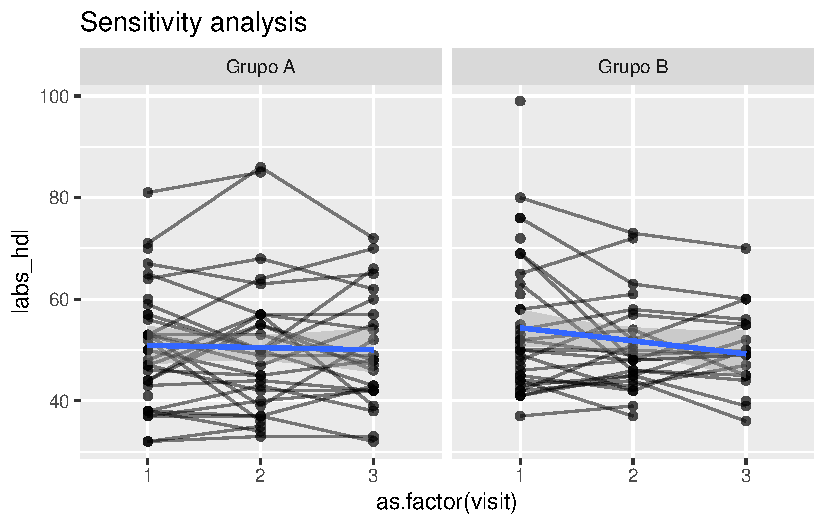
\includegraphics{Outcomes_V1V2V3_files/figure-pdf/labs_hdl_6-2.pdf}

\begin{Shaded}
\begin{Highlighting}[]
    \CommentTok{\#coord\_cartesian(ylim = c(10, 150))}
\end{Highlighting}
\end{Shaded}

\subsubsection{Triglicerídeos}\label{trigliceruxeddeos}

Variável: \texttt{labs\_triglycerides}

\begin{Shaded}
\begin{Highlighting}[]
\CommentTok{\# Plot 1: Raw data}
\NormalTok{labs\_triglycerides\_hist\_1 }\OtherTok{\textless{}{-}}\NormalTok{ data\_model }\SpecialCharTok{\%\textgreater{}\%} 
    \CommentTok{\#filter(}
    \CommentTok{\#    labs\_triglycerides \textless{} 300}
    \CommentTok{\#) \%\textgreater{}\% }
    \FunctionTok{ggplot}\NormalTok{(}\FunctionTok{aes}\NormalTok{(}\AttributeTok{x =}\NormalTok{ labs\_triglycerides)) }\SpecialCharTok{+} 
    \FunctionTok{geom\_histogram}\NormalTok{(}\AttributeTok{bins =} \DecValTok{50}\NormalTok{, }\AttributeTok{fill =} \StringTok{"skyblue"}\NormalTok{, }\AttributeTok{color =} \StringTok{"black"}\NormalTok{)}

\CommentTok{\# Plot 2: Log{-}transformed data}
\NormalTok{labs\_triglycerides\_hist\_2 }\OtherTok{\textless{}{-}}\NormalTok{ data\_model }\SpecialCharTok{\%\textgreater{}\%} 
    \CommentTok{\#filter(}
    \CommentTok{\#    labs\_triglycerides \textless{} 300}
    \CommentTok{\#) \%\textgreater{}\%}
    \FunctionTok{ggplot}\NormalTok{(}\FunctionTok{aes}\NormalTok{(}\AttributeTok{x =} \FunctionTok{log1p}\NormalTok{(labs\_triglycerides))) }\SpecialCharTok{+} 
    \FunctionTok{geom\_histogram}\NormalTok{(}\AttributeTok{bins =} \DecValTok{50}\NormalTok{, }\AttributeTok{fill =} \StringTok{"lightgreen"}\NormalTok{, }\AttributeTok{color =} \StringTok{"black"}\NormalTok{)}

\CommentTok{\# Combine side by side}
\NormalTok{labs\_triglycerides\_hist\_1 }\SpecialCharTok{+}\NormalTok{ labs\_triglycerides\_hist\_2 }\CommentTok{\# library(patchwork)}
\end{Highlighting}
\end{Shaded}

\begin{verbatim}
Warning: Removed 10 rows containing non-finite outside the scale range (`stat_bin()`).
Removed 10 rows containing non-finite outside the scale range (`stat_bin()`).
\end{verbatim}

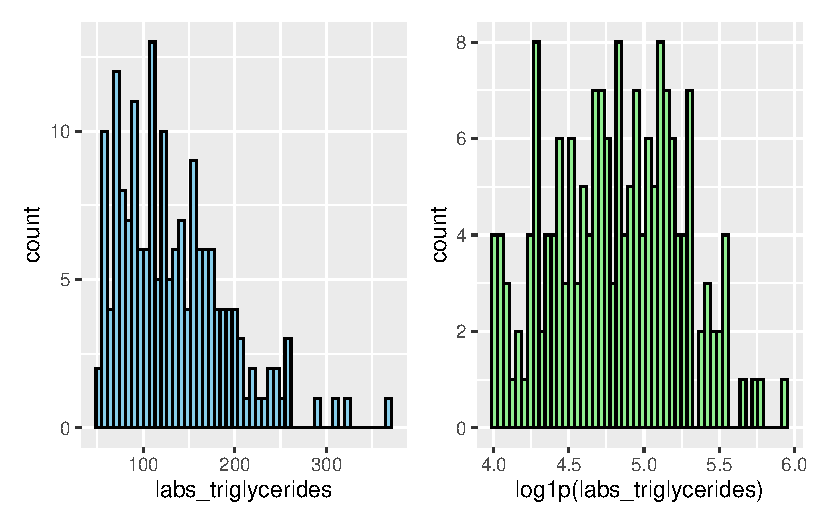
\includegraphics{Outcomes_V1V2V3_files/figure-pdf/labs_triglycerides_1-1.pdf}

\begin{Shaded}
\begin{Highlighting}[]
\CommentTok{\# LMM}
\NormalTok{labs\_triglycerides\_model }\OtherTok{\textless{}{-}} \FunctionTok{lmer}\NormalTok{(}\FunctionTok{log1p}\NormalTok{(labs\_triglycerides) }\SpecialCharTok{\textasciitilde{}}\NormalTok{ allocation\_group }\SpecialCharTok{*}\NormalTok{ visit }\SpecialCharTok{+}\NormalTok{ (}\DecValTok{1} \SpecialCharTok{|}\NormalTok{ record\_id), }\AttributeTok{data =}\NormalTok{ data\_model)}
\FunctionTok{check\_collinearity}\NormalTok{(labs\_triglycerides\_model)}
\end{Highlighting}
\end{Shaded}

\begin{verbatim}
# Check for Multicollinearity

Low Correlation

                   Term  VIF   VIF 95% CI Increased SE Tolerance
       allocation_group 1.20 [1.08, 1.53]         1.10      0.83
                  visit 3.50 [2.79, 4.49]         1.87      0.29
 allocation_group:visit 3.82 [3.03, 4.92]         1.95      0.26
 Tolerance 95% CI
     [0.65, 0.93]
     [0.22, 0.36]
     [0.20, 0.33]
\end{verbatim}

\begin{Shaded}
\begin{Highlighting}[]
\CommentTok{\# Sensitivity analysis}
\NormalTok{labs\_triglycerides\_model\_check }\OtherTok{\textless{}{-}} \FunctionTok{sensitivity\_check\_lmer}\NormalTok{(}
    \AttributeTok{model =}\NormalTok{ labs\_triglycerides\_model,}
    \AttributeTok{id\_var =} \StringTok{"record\_id"}\NormalTok{,}
    \AttributeTok{top\_n =} \DecValTok{5}\NormalTok{)}

\CommentTok{\# LMM Sensitivity}
\NormalTok{labs\_triglycerides\_model\_sens }\OtherTok{\textless{}{-}} \FunctionTok{update}\NormalTok{(}\AttributeTok{object =}\NormalTok{ labs\_triglycerides\_model,}
                              \AttributeTok{subset =} \SpecialCharTok{!}\NormalTok{(record\_id }\SpecialCharTok{\%in\%}\NormalTok{ labs\_triglycerides\_model\_check}\SpecialCharTok{$}\NormalTok{influential\_ids))}
\CommentTok{\# Influential IDS}
\NormalTok{labs\_triglycerides\_model\_check}\SpecialCharTok{$}\NormalTok{influential\_ids}
\end{Highlighting}
\end{Shaded}

\begin{verbatim}
[1] "16" "17" "1"  "2"  "20"
\end{verbatim}

\paragraph{Resumo dos modelos}\label{resumo-dos-modelos-7}

\begin{Shaded}
\begin{Highlighting}[]
\CommentTok{\# Model comparison}
\FunctionTok{summary}\NormalTok{(labs\_triglycerides\_model)}
\end{Highlighting}
\end{Shaded}

\begin{verbatim}
Linear mixed model fit by REML. t-tests use Satterthwaite's method [
lmerModLmerTest]
Formula: log1p(labs_triglycerides) ~ allocation_group * visit + (1 | record_id)
   Data: data_model

REML criterion at convergence: 156.5

Scaled residuals: 
     Min       1Q   Median       3Q      Max 
-2.48575 -0.55624 -0.06875  0.50582  2.77617 

Random effects:
 Groups    Name        Variance Std.Dev.
 record_id (Intercept) 0.12894  0.3591  
 Residual              0.06212  0.2492  
Number of obs: 179, groups:  record_id, 75

Fixed effects:
                                Estimate Std. Error        df t value Pr(>|t|)
(Intercept)                      4.76585    0.07186 100.80805  66.322   <2e-16
allocation_groupGrupo B         -0.02118    0.10095 100.80805  -0.210    0.834
visit2                           0.05652    0.06246 103.24903   0.905    0.368
visit3                           0.00822    0.06765 104.67836   0.122    0.904
allocation_groupGrupo B:visit2  -0.05643    0.09159 105.09618  -0.616    0.539
allocation_groupGrupo B:visit3   0.04983    0.09836 106.17407   0.507    0.614
                                  
(Intercept)                    ***
allocation_groupGrupo B           
visit2                            
visit3                            
allocation_groupGrupo B:visit2    
allocation_groupGrupo B:visit3    
---
Signif. codes:  0 '***' 0.001 '**' 0.01 '*' 0.05 '.' 0.1 ' ' 1

Correlation of Fixed Effects:
            (Intr) all_GB visit2 visit3 a_GB:2
allctn_grGB -0.712                            
visit2      -0.374  0.266                     
visit3      -0.345  0.246  0.449              
allctn_GB:2  0.255 -0.358 -0.682 -0.306       
allctn_GB:3  0.238 -0.334 -0.309 -0.688  0.433
\end{verbatim}

\begin{Shaded}
\begin{Highlighting}[]
\FunctionTok{summary}\NormalTok{(labs\_triglycerides\_model\_sens)}
\end{Highlighting}
\end{Shaded}

\begin{verbatim}
Linear mixed model fit by REML. t-tests use Satterthwaite's method [
lmerModLmerTest]
Formula: log1p(labs_triglycerides) ~ allocation_group * visit + (1 | record_id)
   Data: data_model
 Subset: !(record_id %in% labs_triglycerides_model_check$influential_ids)

REML criterion at convergence: 110.8

Scaled residuals: 
     Min       1Q   Median       3Q      Max 
-1.56781 -0.62311 -0.09172  0.57450  2.18137 

Random effects:
 Groups    Name        Variance Std.Dev.
 record_id (Intercept) 0.12547  0.3542  
 Residual              0.04498  0.2121  
Number of obs: 164, groups:  record_id, 70

Fixed effects:
                               Estimate Std. Error       df t value Pr(>|t|)
(Intercept)                     4.74183    0.07187 86.86729  65.980   <2e-16
allocation_groupGrupo B        -0.02502    0.09885 86.86729  -0.253   0.8008
visit2                          0.04807    0.05702 92.31050   0.843   0.4014
visit3                         -0.09539    0.06269 93.35327  -1.522   0.1314
allocation_groupGrupo B:visit2 -0.01744    0.08158 93.47289  -0.214   0.8312
allocation_groupGrupo B:visit3  0.17857    0.08845 94.22579   2.019   0.0463
                                  
(Intercept)                    ***
allocation_groupGrupo B           
visit2                            
visit3                            
allocation_groupGrupo B:visit2    
allocation_groupGrupo B:visit3 *  
---
Signif. codes:  0 '***' 0.001 '**' 0.01 '*' 0.05 '.' 0.1 ' ' 1

Correlation of Fixed Effects:
            (Intr) all_GB visit2 visit3 a_GB:2
allctn_grGB -0.727                            
visit2      -0.333  0.242                     
visit3      -0.303  0.220  0.444              
allctn_GB:2  0.232 -0.320 -0.699 -0.310       
allctn_GB:3  0.214 -0.295 -0.314 -0.709  0.431
\end{verbatim}

\begin{Shaded}
\begin{Highlighting}[]
\NormalTok{labs\_triglycerides\_model\_check}\SpecialCharTok{$}\NormalTok{comparison\_table}
\end{Highlighting}
\end{Shaded}

\begin{verbatim}
# A tibble: 16 x 6
   Model       term                       estimate std.error statistic   p.value
   <chr>       <chr>                         <dbl>     <dbl>     <dbl>     <dbl>
 1 Original    (Intercept)                 4.77       0.0719    66.3    5.68e-85
 2 Sensitivity (Intercept)                 4.74       0.0719    66.0    5.34e-76
 3 Original    allocation_groupGrupo B    -0.0212     0.101     -0.210  8.34e- 1
 4 Sensitivity allocation_groupGrupo B    -0.0250     0.0989    -0.253  8.01e- 1
 5 Original    allocation_groupGrupo B:v~ -0.0564     0.0916    -0.616  5.39e- 1
 6 Sensitivity allocation_groupGrupo B:v~ -0.0174     0.0816    -0.214  8.31e- 1
 7 Original    allocation_groupGrupo B:v~  0.0498     0.0984     0.507  6.14e- 1
 8 Sensitivity allocation_groupGrupo B:v~  0.179      0.0884     2.02   4.63e- 2
 9 Original    sd__(Intercept)             0.359     NA         NA     NA       
10 Sensitivity sd__(Intercept)             0.354     NA         NA     NA       
11 Original    sd__Observation             0.249     NA         NA     NA       
12 Sensitivity sd__Observation             0.212     NA         NA     NA       
13 Original    visit2                      0.0565     0.0625     0.905  3.68e- 1
14 Sensitivity visit2                      0.0481     0.0570     0.843  4.01e- 1
15 Original    visit3                      0.00822    0.0677     0.122  9.04e- 1
16 Sensitivity visit3                     -0.0954     0.0627    -1.52   1.31e- 1
\end{verbatim}

\begin{Shaded}
\begin{Highlighting}[]
\NormalTok{performance}\SpecialCharTok{::}\FunctionTok{compare\_performance}\NormalTok{(labs\_triglycerides\_model, labs\_triglycerides\_model\_sens)}
\end{Highlighting}
\end{Shaded}

\begin{verbatim}
When comparing models, please note that probably not all models were fit
  from same data.
\end{verbatim}

\begin{verbatim}
# Comparison of Model Performance Indices

Name                          |           Model |  AIC (weights)
----------------------------------------------------------------
labs_triglycerides_model      | lmerModLmerTest | 1873.1 (<.001)
labs_triglycerides_model_sens | lmerModLmerTest | 1671.7 (>.999)

Name                          | AICc (weights) |  BIC (weights) | R2 (cond.)
----------------------------------------------------------------------------
labs_triglycerides_model      | 1873.9 (<.001) | 1898.6 (<.001) |      0.676
labs_triglycerides_model_sens | 1672.6 (>.999) | 1696.5 (>.999) |      0.739

Name                          | R2 (marg.) |   ICC |  RMSE | Sigma
------------------------------------------------------------------
labs_triglycerides_model      |      0.004 | 0.675 | 0.199 | 0.249
labs_triglycerides_model_sens |      0.012 | 0.736 | 0.166 | 0.212
\end{verbatim}

\begin{Shaded}
\begin{Highlighting}[]
\NormalTok{performance}\SpecialCharTok{::}\FunctionTok{check\_model}\NormalTok{(labs\_triglycerides\_model)}
\end{Highlighting}
\end{Shaded}

\includegraphics{Outcomes_V1V2V3_files/figure-pdf/labs_triglycerides_4-1.pdf}

\begin{Shaded}
\begin{Highlighting}[]
\NormalTok{performance}\SpecialCharTok{::}\FunctionTok{check\_model}\NormalTok{(labs\_triglycerides\_model\_sens)}
\end{Highlighting}
\end{Shaded}

\includegraphics{Outcomes_V1V2V3_files/figure-pdf/labs_triglycerides_4-2.pdf}

\paragraph{Médias Marginais
Estimadas}\label{muxe9dias-marginais-estimadas-7}

\begin{Shaded}
\begin{Highlighting}[]
\CommentTok{\# Get EMMs for each group at each visit}
\NormalTok{labs\_triglycerides\_raw\_emm }\OtherTok{\textless{}{-}}\NormalTok{ emmeans}\SpecialCharTok{::}\FunctionTok{emmeans}\NormalTok{(}
\NormalTok{    labs\_triglycerides\_model, }
    \SpecialCharTok{\textasciitilde{}}\NormalTok{ allocation\_group }\SpecialCharTok{*}\NormalTok{ visit}
\NormalTok{)}

\NormalTok{labs\_triglycerides\_raw\_emm }\OtherTok{\textless{}{-}} \FunctionTok{regrid}\NormalTok{(labs\_triglycerides\_raw\_emm)}

\CommentTok{\# Table of marginal means}
\NormalTok{labs\_triglycerides\_raw\_emm}
\end{Highlighting}
\end{Shaded}

\begin{verbatim}
 allocation_group visit response    SE  df lower.CL upper.CL
 Grupo A          1          116  8.44 103     99.7      133
 Grupo B          1          114  8.15 103     97.8      130
 Grupo A          2          123  9.39 116    104.7      142
 Grupo B          2          114  9.10 132     96.0      132
 Grupo A          3          117  9.47 133     98.7      136
 Grupo B          3          121 10.10 145    100.9      141

Degrees-of-freedom method: inherited from kenward-roger when re-gridding 
Confidence level used: 0.95 
\end{verbatim}

\begin{Shaded}
\begin{Highlighting}[]
\CommentTok{\# Pairwise comparisons: Between groups at each visit}
\NormalTok{emmeans}\SpecialCharTok{::}\FunctionTok{contrast}\NormalTok{(labs\_triglycerides\_raw\_emm, }\AttributeTok{method =} \StringTok{"pairwise"}\NormalTok{, }\AttributeTok{by =} \StringTok{"visit"}\NormalTok{, }\AttributeTok{adjust =} \StringTok{"bonferroni"}\NormalTok{) }\SpecialCharTok{\%\textgreater{}\%} \FunctionTok{summary}\NormalTok{(}\AttributeTok{infer =} \FunctionTok{c}\NormalTok{(}\ConstantTok{TRUE}\NormalTok{, }\ConstantTok{TRUE}\NormalTok{))}
\end{Highlighting}
\end{Shaded}

\begin{verbatim}
visit = 1:
 contrast          estimate   SE  df lower.CL upper.CL t.ratio p.value
 Grupo A - Grupo B     2.46 11.7 103    -20.8     25.7   0.210  0.8343

visit = 2:
 contrast          estimate   SE  df lower.CL upper.CL t.ratio p.value
 Grupo A - Grupo B     9.28 13.1 116    -16.6     35.2   0.710  0.4793

visit = 3:
 contrast          estimate   SE  df lower.CL upper.CL t.ratio p.value
 Grupo A - Grupo B    -3.44 13.8 133    -30.8     23.9  -0.249  0.8041

Degrees-of-freedom method: inherited from kenward-roger when re-gridding 
Confidence level used: 0.95 
\end{verbatim}

\begin{Shaded}
\begin{Highlighting}[]
\CommentTok{\# Pairwise comparisons: Changes over time within each group}
\NormalTok{emmeans}\SpecialCharTok{::}\FunctionTok{contrast}\NormalTok{(labs\_triglycerides\_raw\_emm, }\AttributeTok{method =} \StringTok{"pairwise"}\NormalTok{, }\AttributeTok{by =} \StringTok{"allocation\_group"}\NormalTok{, }\AttributeTok{adjust =} \StringTok{"bonferroni"}\NormalTok{) }\SpecialCharTok{\%\textgreater{}\%} \FunctionTok{summary}\NormalTok{(}\AttributeTok{infer =} \FunctionTok{c}\NormalTok{(}\ConstantTok{TRUE}\NormalTok{, }\ConstantTok{TRUE}\NormalTok{))}
\end{Highlighting}
\end{Shaded}

\begin{verbatim}
allocation_group = Grupo A:
 contrast        estimate   SE  df lower.CL upper.CL t.ratio p.value
 visit1 - visit2 -6.82768 7.60 103    -25.3     11.7  -0.899  1.0000
 visit1 - visit3 -0.96930 8.00 103    -20.4     18.5  -0.121  1.0000
 visit2 - visit3  5.85838 8.29 116    -14.3     26.0   0.707  1.0000

allocation_group = Grupo B:
 contrast        estimate   SE  df lower.CL upper.CL t.ratio p.value
 visit1 - visit2 -0.00919 7.71 103    -18.8     18.8  -0.001  1.0000
 visit1 - visit3 -6.87130 8.57 103    -27.7     14.0  -0.802  1.0000
 visit2 - visit3 -6.86211 8.90 132    -28.4     14.7  -0.771  1.0000

Degrees-of-freedom method: inherited from kenward-roger when re-gridding 
Confidence level used: 0.95 
Conf-level adjustment: bonferroni method for 3 estimates 
P value adjustment: bonferroni method for 3 tests 
\end{verbatim}

\begin{Shaded}
\begin{Highlighting}[]
\CommentTok{\# Plot of marginal means}
\FunctionTok{plot}\NormalTok{(labs\_triglycerides\_raw\_emm, }\AttributeTok{comparisons =} \ConstantTok{TRUE}\NormalTok{)}
\end{Highlighting}
\end{Shaded}

\includegraphics{Outcomes_V1V2V3_files/figure-pdf/labs_triglycerides_raw_emm-1.pdf}

\begin{Shaded}
\begin{Highlighting}[]
\CommentTok{\# Get EMMs for each group at each visit}
\NormalTok{labs\_triglycerides\_emm }\OtherTok{\textless{}{-}}\NormalTok{ emmeans}\SpecialCharTok{::}\FunctionTok{emmeans}\NormalTok{(}
\NormalTok{    labs\_triglycerides\_model\_sens, }
    \SpecialCharTok{\textasciitilde{}}\NormalTok{ allocation\_group }\SpecialCharTok{*}\NormalTok{ visit}
\NormalTok{)}

\NormalTok{labs\_triglycerides\_emm }\OtherTok{\textless{}{-}} \FunctionTok{regrid}\NormalTok{(labs\_triglycerides\_emm)}

\CommentTok{\# Table of marginal means}
\NormalTok{labs\_triglycerides\_emm}
\end{Highlighting}
\end{Shaded}

\begin{verbatim}
 allocation_group visit response   SE    df lower.CL upper.CL
 Grupo A          1          114 8.24  88.9     97.3      130
 Grupo B          1          111 7.59  88.9     95.7      126
 Grupo A          2          119 9.08 101.6    101.3      137
 Grupo B          2          114 8.62 114.3     97.2      131
 Grupo A          3          103 8.32 117.7     86.7      120
 Grupo B          3          121 9.48 125.6    101.8      139

Degrees-of-freedom method: inherited from kenward-roger when re-gridding 
Confidence level used: 0.95 
\end{verbatim}

\begin{Shaded}
\begin{Highlighting}[]
\CommentTok{\# Pairwise comparisons: Between groups at each visit}
\NormalTok{emmeans}\SpecialCharTok{::}\FunctionTok{contrast}\NormalTok{(labs\_triglycerides\_emm, }\AttributeTok{method =} \StringTok{"pairwise"}\NormalTok{, }\AttributeTok{by =} \StringTok{"visit"}\NormalTok{, }\AttributeTok{adjust =} \StringTok{"bonferroni"}\NormalTok{) }\SpecialCharTok{\%\textgreater{}\%} \FunctionTok{summary}\NormalTok{(}\AttributeTok{infer =} \FunctionTok{c}\NormalTok{(}\ConstantTok{TRUE}\NormalTok{, }\ConstantTok{TRUE}\NormalTok{))}
\end{Highlighting}
\end{Shaded}

\begin{verbatim}
visit = 1:
 contrast          estimate   SE    df lower.CL upper.CL t.ratio p.value
 Grupo A - Grupo B     2.83 11.2  88.9    -19.4    25.09   0.253  0.8010

visit = 2:
 contrast          estimate   SE    df lower.CL upper.CL t.ratio p.value
 Grupo A - Grupo B     5.00 12.5 101.6    -19.8    29.83   0.399  0.6904

visit = 3:
 contrast          estimate   SE    df lower.CL upper.CL t.ratio p.value
 Grupo A - Grupo B   -17.30 12.6 117.7    -42.3     7.68  -1.371  0.1729

Degrees-of-freedom method: inherited from kenward-roger when re-gridding 
Confidence level used: 0.95 
\end{verbatim}

\begin{Shaded}
\begin{Highlighting}[]
\CommentTok{\# Pairwise comparisons: Changes over time within each group}
\NormalTok{emmeans}\SpecialCharTok{::}\FunctionTok{contrast}\NormalTok{(labs\_triglycerides\_emm, }\AttributeTok{method =} \StringTok{"pairwise"}\NormalTok{, }\AttributeTok{by =} \StringTok{"allocation\_group"}\NormalTok{, }\AttributeTok{adjust =} \StringTok{"bonferroni"}\NormalTok{) }\SpecialCharTok{\%\textgreater{}\%} \FunctionTok{summary}\NormalTok{(}\AttributeTok{infer =} \FunctionTok{c}\NormalTok{(}\ConstantTok{TRUE}\NormalTok{, }\ConstantTok{TRUE}\NormalTok{))}
\end{Highlighting}
\end{Shaded}

\begin{verbatim}
allocation_group = Grupo A:
 contrast        estimate   SE    df lower.CL upper.CL t.ratio p.value
 visit1 - visit2    -5.65 6.74  88.9   -22.10    10.81  -0.837  1.0000
 visit1 - visit3    10.43 6.81  88.9    -6.17    27.04   1.533  0.3866
 visit2 - visit3    16.08 7.12 101.6    -1.25    33.40   2.259  0.0780

allocation_group = Grupo B:
 contrast        estimate   SE    df lower.CL upper.CL t.ratio p.value
 visit1 - visit2    -3.48 6.67  88.9   -19.75    12.79  -0.522  1.0000
 visit1 - visit3    -9.70 7.43  88.9   -27.83     8.44  -1.305  0.5861
 visit2 - visit3    -6.22 7.76 114.3   -25.07    12.63  -0.802  1.0000

Degrees-of-freedom method: inherited from kenward-roger when re-gridding 
Confidence level used: 0.95 
Conf-level adjustment: bonferroni method for 3 estimates 
P value adjustment: bonferroni method for 3 tests 
\end{verbatim}

\begin{Shaded}
\begin{Highlighting}[]
\CommentTok{\# Plot of marginal means}
\FunctionTok{plot}\NormalTok{(labs\_triglycerides\_emm, }\AttributeTok{comparisons =} \ConstantTok{TRUE}\NormalTok{)}
\end{Highlighting}
\end{Shaded}

\includegraphics{Outcomes_V1V2V3_files/figure-pdf/labs_triglycerides_sens_emm-1.pdf}

\begin{Shaded}
\begin{Highlighting}[]
\FunctionTok{ggplot}\NormalTok{(}
    \AttributeTok{data =}\NormalTok{ data\_model, }
    \FunctionTok{aes}\NormalTok{(}
        \AttributeTok{x =} \FunctionTok{as.factor}\NormalTok{(visit),}
        \AttributeTok{y =}\NormalTok{ labs\_triglycerides,}
        \AttributeTok{group =}\NormalTok{ record\_id,}
\NormalTok{    )}
\NormalTok{) }\SpecialCharTok{+}
    \FunctionTok{geom\_line}\NormalTok{(}\AttributeTok{alpha =} \FloatTok{0.5}\NormalTok{) }\SpecialCharTok{+}
    \FunctionTok{geom\_point}\NormalTok{(}\AttributeTok{alpha =} \FloatTok{0.7}\NormalTok{) }\SpecialCharTok{+}
    \FunctionTok{geom\_smooth}\NormalTok{(}
        \FunctionTok{aes}\NormalTok{(}\AttributeTok{group =}\NormalTok{ allocation\_group),}
        \AttributeTok{method =} \StringTok{"lm"}\NormalTok{,}
        \AttributeTok{se =} \ConstantTok{TRUE}\NormalTok{,}
        \AttributeTok{linewidth =} \DecValTok{1}
\NormalTok{    ) }\SpecialCharTok{+}
    \FunctionTok{labs}\NormalTok{(}\AttributeTok{title =} \StringTok{"All data"}\NormalTok{) }\SpecialCharTok{+}
    \FunctionTok{facet\_wrap}\NormalTok{(}\SpecialCharTok{\textasciitilde{}}\NormalTok{ allocation\_group) }
\end{Highlighting}
\end{Shaded}

\begin{verbatim}
`geom_smooth()` using formula = 'y ~ x'
\end{verbatim}

\begin{verbatim}
Warning: Removed 10 rows containing non-finite outside the scale range
(`stat_smooth()`).
\end{verbatim}

\begin{verbatim}
Warning: Removed 8 rows containing missing values or values outside the scale range
(`geom_line()`).
\end{verbatim}

\begin{verbatim}
Warning: Removed 10 rows containing missing values or values outside the scale range
(`geom_point()`).
\end{verbatim}

\includegraphics{Outcomes_V1V2V3_files/figure-pdf/labs_triglycerides_6-1.pdf}

\begin{Shaded}
\begin{Highlighting}[]
    \CommentTok{\#coord\_cartesian(ylim = c(10, 150))}

\NormalTok{data\_model }\SpecialCharTok{\%\textgreater{}\%} 
    \FunctionTok{filter}\NormalTok{(}
        \SpecialCharTok{!}\NormalTok{(record\_id }\SpecialCharTok{\%in\%}\NormalTok{ labs\_triglycerides\_model\_check}\SpecialCharTok{$}\NormalTok{influential\_ids)}
\NormalTok{    ) }\SpecialCharTok{\%\textgreater{}\%} 
    \FunctionTok{ggplot}\NormalTok{(}
        \FunctionTok{aes}\NormalTok{(}
            \AttributeTok{x =} \FunctionTok{as.factor}\NormalTok{(visit),}
            \AttributeTok{y =}\NormalTok{ labs\_triglycerides,}
            \AttributeTok{group =}\NormalTok{ record\_id,}
\NormalTok{        )}
\NormalTok{    ) }\SpecialCharTok{+}
    \FunctionTok{geom\_line}\NormalTok{(}\AttributeTok{alpha =} \FloatTok{0.5}\NormalTok{) }\SpecialCharTok{+}
    \FunctionTok{geom\_point}\NormalTok{(}\AttributeTok{alpha =} \FloatTok{0.7}\NormalTok{) }\SpecialCharTok{+}
    \FunctionTok{geom\_smooth}\NormalTok{(}
        \FunctionTok{aes}\NormalTok{(}\AttributeTok{group =}\NormalTok{ allocation\_group),}
        \AttributeTok{method =} \StringTok{"lm"}\NormalTok{,}
        \AttributeTok{se =} \ConstantTok{TRUE}\NormalTok{,}
        \AttributeTok{linewidth =} \DecValTok{1}
\NormalTok{    ) }\SpecialCharTok{+}
    \FunctionTok{labs}\NormalTok{(}\AttributeTok{title =} \StringTok{"Sensitivity analysis"}\NormalTok{) }\SpecialCharTok{+}
    \FunctionTok{facet\_wrap}\NormalTok{(}\SpecialCharTok{\textasciitilde{}}\NormalTok{ allocation\_group) }
\end{Highlighting}
\end{Shaded}

\begin{verbatim}
`geom_smooth()` using formula = 'y ~ x'
\end{verbatim}

\begin{verbatim}
Warning: Removed 10 rows containing non-finite outside the scale range
(`stat_smooth()`).
\end{verbatim}

\begin{verbatim}
Warning: Removed 8 rows containing missing values or values outside the scale range
(`geom_line()`).
\end{verbatim}

\begin{verbatim}
Warning: Removed 10 rows containing missing values or values outside the scale range
(`geom_point()`).
\end{verbatim}

\includegraphics{Outcomes_V1V2V3_files/figure-pdf/labs_triglycerides_6-2.pdf}

\begin{Shaded}
\begin{Highlighting}[]
    \CommentTok{\#coord\_cartesian(ylim = c(10, 150))}
\end{Highlighting}
\end{Shaded}

\subsubsection{Glicemia de jejum}\label{glicemia-de-jejum}

Variável: \texttt{labs\_glucose}

\begin{Shaded}
\begin{Highlighting}[]
\CommentTok{\# Plot 1: Raw data}
\NormalTok{labs\_glucose\_hist\_1 }\OtherTok{\textless{}{-}}\NormalTok{ data\_model }\SpecialCharTok{\%\textgreater{}\%} 
    \CommentTok{\#filter(}
    \CommentTok{\#    labs\_glucose \textless{} 300}
    \CommentTok{\#) \%\textgreater{}\% }
    \FunctionTok{ggplot}\NormalTok{(}\FunctionTok{aes}\NormalTok{(}\AttributeTok{x =}\NormalTok{ labs\_glucose)) }\SpecialCharTok{+} 
    \FunctionTok{geom\_histogram}\NormalTok{(}\AttributeTok{bins =} \DecValTok{50}\NormalTok{, }\AttributeTok{fill =} \StringTok{"skyblue"}\NormalTok{, }\AttributeTok{color =} \StringTok{"black"}\NormalTok{)}

\CommentTok{\# Plot 2: Log{-}transformed data}
\NormalTok{labs\_glucose\_hist\_2 }\OtherTok{\textless{}{-}}\NormalTok{ data\_model }\SpecialCharTok{\%\textgreater{}\%} 
    \CommentTok{\#filter(}
    \CommentTok{\#    labs\_glucose \textless{} 300}
    \CommentTok{\#) \%\textgreater{}\%}
    \FunctionTok{ggplot}\NormalTok{(}\FunctionTok{aes}\NormalTok{(}\AttributeTok{x =} \FunctionTok{log1p}\NormalTok{(labs\_glucose))) }\SpecialCharTok{+} 
    \FunctionTok{geom\_histogram}\NormalTok{(}\AttributeTok{bins =} \DecValTok{50}\NormalTok{, }\AttributeTok{fill =} \StringTok{"lightgreen"}\NormalTok{, }\AttributeTok{color =} \StringTok{"black"}\NormalTok{)}

\CommentTok{\# Combine side by side}
\NormalTok{labs\_glucose\_hist\_1 }\SpecialCharTok{+}\NormalTok{ labs\_glucose\_hist\_2 }\CommentTok{\# library(patchwork)}
\end{Highlighting}
\end{Shaded}

\begin{verbatim}
Warning: Removed 13 rows containing non-finite outside the scale range (`stat_bin()`).
Removed 13 rows containing non-finite outside the scale range (`stat_bin()`).
\end{verbatim}

\includegraphics{Outcomes_V1V2V3_files/figure-pdf/labs_glucose_1-1.pdf}

\begin{Shaded}
\begin{Highlighting}[]
\CommentTok{\# LMM}
\NormalTok{labs\_glucose\_model }\OtherTok{\textless{}{-}} \FunctionTok{lmer}\NormalTok{(}\FunctionTok{log1p}\NormalTok{(labs\_glucose) }\SpecialCharTok{\textasciitilde{}}\NormalTok{ allocation\_group }\SpecialCharTok{*}\NormalTok{ visit }\SpecialCharTok{+}\NormalTok{ (}\DecValTok{1} \SpecialCharTok{|}\NormalTok{ record\_id), }\AttributeTok{data =}\NormalTok{ data\_model)}
\FunctionTok{check\_collinearity}\NormalTok{(labs\_glucose\_model)}
\end{Highlighting}
\end{Shaded}

\begin{verbatim}
# Check for Multicollinearity

Low Correlation

                   Term  VIF   VIF 95% CI Increased SE Tolerance
       allocation_group 1.13 [1.03, 1.51]         1.06      0.89
                  visit 3.47 [2.76, 4.47]         1.86      0.29
 allocation_group:visit 3.69 [2.93, 4.75]         1.92      0.27
 Tolerance 95% CI
     [0.66, 0.97]
     [0.22, 0.36]
     [0.21, 0.34]
\end{verbatim}

\begin{Shaded}
\begin{Highlighting}[]
\CommentTok{\# Sensitivity analysis}
\NormalTok{labs\_glucose\_model\_check }\OtherTok{\textless{}{-}} \FunctionTok{sensitivity\_check\_lmer}\NormalTok{(}
    \AttributeTok{model =}\NormalTok{ labs\_glucose\_model,}
    \AttributeTok{id\_var =} \StringTok{"record\_id"}\NormalTok{,}
    \AttributeTok{top\_n =} \DecValTok{5}\NormalTok{)}

\CommentTok{\# LMM Sensitivity}
\NormalTok{labs\_glucose\_model\_sens }\OtherTok{\textless{}{-}} \FunctionTok{update}\NormalTok{(}\AttributeTok{object =}\NormalTok{ labs\_glucose\_model,}
                              \AttributeTok{subset =} \SpecialCharTok{!}\NormalTok{(record\_id }\SpecialCharTok{\%in\%}\NormalTok{ labs\_glucose\_model\_check}\SpecialCharTok{$}\NormalTok{influential\_ids))}
\CommentTok{\# Influential IDS}
\NormalTok{labs\_glucose\_model\_check}\SpecialCharTok{$}\NormalTok{influential\_ids}
\end{Highlighting}
\end{Shaded}

\begin{verbatim}
[1] "2"  "16" "17" "56" "13"
\end{verbatim}

\paragraph{Resumo dos modelos}\label{resumo-dos-modelos-8}

\begin{Shaded}
\begin{Highlighting}[]
\CommentTok{\# Model comparison}
\FunctionTok{summary}\NormalTok{(labs\_glucose\_model)}
\end{Highlighting}
\end{Shaded}

\begin{verbatim}
Linear mixed model fit by REML. t-tests use Satterthwaite's method [
lmerModLmerTest]
Formula: log1p(labs_glucose) ~ allocation_group * visit + (1 | record_id)
   Data: data_model

REML criterion at convergence: -153

Scaled residuals: 
    Min      1Q  Median      3Q     Max 
-2.0712 -0.5250 -0.1192  0.4737  3.4423 

Random effects:
 Groups    Name        Variance Std.Dev.
 record_id (Intercept) 0.030440 0.17447 
 Residual              0.008319 0.09121 
Number of obs: 176, groups:  record_id, 74

Fixed effects:
                                 Estimate Std. Error         df t value
(Intercept)                      4.445812   0.032366  92.773372 137.362
allocation_groupGrupo B          0.002937   0.045895  93.526588   0.064
visit2                           0.009144   0.023244 104.438133   0.393
visit3                           0.035792   0.024905 105.095812   1.437
allocation_groupGrupo B:visit2  -0.019077   0.034014 105.360265  -0.561
allocation_groupGrupo B:visit3  -0.007509   0.036617 106.709642  -0.205
                               Pr(>|t|)    
(Intercept)                      <2e-16 ***
allocation_groupGrupo B           0.949    
visit2                            0.695    
visit3                            0.154    
allocation_groupGrupo B:visit2    0.576    
allocation_groupGrupo B:visit3    0.838    
---
Signif. codes:  0 '***' 0.001 '**' 0.01 '*' 0.05 '.' 0.1 ' ' 1

Correlation of Fixed Effects:
            (Intr) all_GB visit2 visit3 a_GB:2
allctn_grGB -0.705                            
visit2      -0.299  0.211                     
visit3      -0.279  0.197  0.445              
allctn_GB:2  0.204 -0.293 -0.683 -0.304       
allctn_GB:3  0.190 -0.278 -0.303 -0.680  0.439
\end{verbatim}

\begin{Shaded}
\begin{Highlighting}[]
\FunctionTok{summary}\NormalTok{(labs\_glucose\_model\_sens)}
\end{Highlighting}
\end{Shaded}

\begin{verbatim}
Linear mixed model fit by REML. t-tests use Satterthwaite's method [
lmerModLmerTest]
Formula: log1p(labs_glucose) ~ allocation_group * visit + (1 | record_id)
   Data: data_model
 Subset: !(record_id %in% labs_glucose_model_check$influential_ids)

REML criterion at convergence: -224.4

Scaled residuals: 
    Min      1Q  Median      3Q     Max 
-1.9874 -0.5692 -0.1200  0.5703  1.9303 

Random effects:
 Groups    Name        Variance Std.Dev.
 record_id (Intercept) 0.011973 0.10942 
 Residual              0.005831 0.07636 
Number of obs: 161, groups:  record_id, 69

Fixed effects:
                                 Estimate Std. Error         df t value
(Intercept)                     4.4198168  0.0228838 96.3391006 193.142
allocation_groupGrupo B        -0.0005277  0.0322590 97.2962023  -0.016
visit2                         -0.0018470  0.0203795 96.0503867  -0.091
visit3                          0.0190546  0.0220059 97.1965932   0.866
allocation_groupGrupo B:visit2 -0.0022058  0.0295835 97.2662772  -0.075
allocation_groupGrupo B:visit3  0.0099619  0.0320363 99.3466017   0.311
                               Pr(>|t|)    
(Intercept)                      <2e-16 ***
allocation_groupGrupo B           0.987    
visit2                            0.928    
visit3                            0.389    
allocation_groupGrupo B:visit2    0.941    
allocation_groupGrupo B:visit3    0.756    
---
Signif. codes:  0 '***' 0.001 '**' 0.01 '*' 0.05 '.' 0.1 ' ' 1

Correlation of Fixed Effects:
            (Intr) all_GB visit2 visit3 a_GB:2
allctn_grGB -0.709                            
visit2      -0.368  0.261                     
visit3      -0.341  0.242  0.435              
allctn_GB:2  0.253 -0.360 -0.689 -0.300       
allctn_GB:3  0.234 -0.339 -0.299 -0.687  0.428
\end{verbatim}

\begin{Shaded}
\begin{Highlighting}[]
\NormalTok{labs\_glucose\_model\_check}\SpecialCharTok{$}\NormalTok{comparison\_table}
\end{Highlighting}
\end{Shaded}

\begin{verbatim}
# A tibble: 16 x 6
   Model       term                      estimate std.error statistic    p.value
   <chr>       <chr>                        <dbl>     <dbl>     <dbl>      <dbl>
 1 Original    (Intercept)                4.45e+0    0.0324  137.      5.55e-109
 2 Sensitivity (Intercept)                4.42e+0    0.0229  193.      1.57e-126
 3 Original    allocation_groupGrupo B    2.94e-3    0.0459    0.0640  9.49e-  1
 4 Sensitivity allocation_groupGrupo B   -5.28e-4    0.0323   -0.0164  9.87e-  1
 5 Original    allocation_groupGrupo B:~ -1.91e-2    0.0340   -0.561   5.76e-  1
 6 Sensitivity allocation_groupGrupo B:~ -2.21e-3    0.0296   -0.0746  9.41e-  1
 7 Original    allocation_groupGrupo B:~ -7.51e-3    0.0366   -0.205   8.38e-  1
 8 Sensitivity allocation_groupGrupo B:~  9.96e-3    0.0320    0.311   7.56e-  1
 9 Original    sd__(Intercept)            1.74e-1   NA        NA      NA        
10 Sensitivity sd__(Intercept)            1.09e-1   NA        NA      NA        
11 Original    sd__Observation            9.12e-2   NA        NA      NA        
12 Sensitivity sd__Observation            7.64e-2   NA        NA      NA        
13 Original    visit2                     9.14e-3    0.0232    0.393   6.95e-  1
14 Sensitivity visit2                    -1.85e-3    0.0204   -0.0906  9.28e-  1
15 Original    visit3                     3.58e-2    0.0249    1.44    1.54e-  1
16 Sensitivity visit3                     1.91e-2    0.0220    0.866   3.89e-  1
\end{verbatim}

\begin{Shaded}
\begin{Highlighting}[]
\NormalTok{performance}\SpecialCharTok{::}\FunctionTok{compare\_performance}\NormalTok{(labs\_glucose\_model, labs\_glucose\_model\_sens)}
\end{Highlighting}
\end{Shaded}

\begin{verbatim}
When comparing models, please note that probably not all models were fit
  from same data.
\end{verbatim}

\begin{verbatim}
# Comparison of Model Performance Indices

Name                    |           Model |  AIC (weights) | AICc (weights)
---------------------------------------------------------------------------
labs_glucose_model      | lmerModLmerTest | 1404.0 (<.001) | 1404.9 (<.001)
labs_glucose_model_sens | lmerModLmerTest | 1183.8 (>.999) | 1184.7 (>.999)

Name                    |  BIC (weights) | R2 (cond.) | R2 (marg.) |   ICC
--------------------------------------------------------------------------
labs_glucose_model      | 1429.4 (<.001) |      0.787 |      0.006 | 0.785
labs_glucose_model_sens | 1208.4 (>.999) |      0.675 |      0.007 | 0.672

Name                    |  RMSE | Sigma
---------------------------------------
labs_glucose_model      | 0.071 | 0.091
labs_glucose_model_sens | 0.061 | 0.076
\end{verbatim}

\begin{Shaded}
\begin{Highlighting}[]
\NormalTok{performance}\SpecialCharTok{::}\FunctionTok{check\_model}\NormalTok{(labs\_glucose\_model)}
\end{Highlighting}
\end{Shaded}

\includegraphics{Outcomes_V1V2V3_files/figure-pdf/labs_glucose_4-1.pdf}

\begin{Shaded}
\begin{Highlighting}[]
\NormalTok{performance}\SpecialCharTok{::}\FunctionTok{check\_model}\NormalTok{(labs\_glucose\_model\_sens)}
\end{Highlighting}
\end{Shaded}

\includegraphics{Outcomes_V1V2V3_files/figure-pdf/labs_glucose_4-2.pdf}

\paragraph{Médias Marginais
Estimadas}\label{muxe9dias-marginais-estimadas-8}

\begin{Shaded}
\begin{Highlighting}[]
\CommentTok{\# Get EMMs for each group at each visit}
\NormalTok{labs\_glucose\_raw\_emm }\OtherTok{\textless{}{-}}\NormalTok{ emmeans}\SpecialCharTok{::}\FunctionTok{emmeans}\NormalTok{(}
\NormalTok{    labs\_glucose\_model, }
    \SpecialCharTok{\textasciitilde{}}\NormalTok{ allocation\_group }\SpecialCharTok{*}\NormalTok{ visit}
\NormalTok{)}

\NormalTok{labs\_glucose\_raw\_emm }\OtherTok{\textless{}{-}} \FunctionTok{regrid}\NormalTok{(labs\_glucose\_raw\_emm)}

\CommentTok{\# Table of marginal means}
\NormalTok{labs\_glucose\_raw\_emm}
\end{Highlighting}
\end{Shaded}

\begin{verbatim}
 allocation_group visit response   SE    df lower.CL upper.CL
 Grupo A          1         84.3 2.76  89.7     78.8     89.8
 Grupo B          1         84.5 2.78  91.2     79.0     90.0
 Grupo A          2         85.1 2.90 101.8     79.3     90.8
 Grupo B          2         83.7 2.95 111.0     77.8     89.5
 Grupo A          3         87.4 3.09 112.6     81.3     93.5
 Grupo B          3         87.0 3.17 121.5     80.7     93.2

Degrees-of-freedom method: inherited from kenward-roger when re-gridding 
Confidence level used: 0.95 
\end{verbatim}

\begin{Shaded}
\begin{Highlighting}[]
\CommentTok{\# Pairwise comparisons: Between groups at each visit}
\NormalTok{emmeans}\SpecialCharTok{::}\FunctionTok{contrast}\NormalTok{(labs\_glucose\_raw\_emm, }\AttributeTok{method =} \StringTok{"pairwise"}\NormalTok{, }\AttributeTok{by =} \StringTok{"visit"}\NormalTok{, }\AttributeTok{adjust =} \StringTok{"bonferroni"}\NormalTok{) }\SpecialCharTok{\%\textgreater{}\%} \FunctionTok{summary}\NormalTok{(}\AttributeTok{infer =} \FunctionTok{c}\NormalTok{(}\ConstantTok{TRUE}\NormalTok{, }\ConstantTok{TRUE}\NormalTok{))}
\end{Highlighting}
\end{Shaded}

\begin{verbatim}
visit = 1:
 contrast          estimate   SE    df lower.CL upper.CL t.ratio p.value
 Grupo A - Grupo B   -0.251 3.92  89.7    -8.04     7.54  -0.064  0.9491

visit = 2:
 contrast          estimate   SE    df lower.CL upper.CL t.ratio p.value
 Grupo A - Grupo B    1.378 4.14 101.8    -6.83     9.59   0.333  0.7399

visit = 3:
 contrast          estimate   SE    df lower.CL upper.CL t.ratio p.value
 Grupo A - Grupo B    0.403 4.42 112.6    -8.36     9.17   0.091  0.9276

Degrees-of-freedom method: inherited from kenward-roger when re-gridding 
Confidence level used: 0.95 
\end{verbatim}

\begin{Shaded}
\begin{Highlighting}[]
\CommentTok{\# Pairwise comparisons: Changes over time within each group}
\NormalTok{emmeans}\SpecialCharTok{::}\FunctionTok{contrast}\NormalTok{(labs\_glucose\_raw\_emm, }\AttributeTok{method =} \StringTok{"pairwise"}\NormalTok{, }\AttributeTok{by =} \StringTok{"allocation\_group"}\NormalTok{, }\AttributeTok{adjust =} \StringTok{"bonferroni"}\NormalTok{) }\SpecialCharTok{\%\textgreater{}\%} \FunctionTok{summary}\NormalTok{(}\AttributeTok{infer =} \FunctionTok{c}\NormalTok{(}\ConstantTok{TRUE}\NormalTok{, }\ConstantTok{TRUE}\NormalTok{))}
\end{Highlighting}
\end{Shaded}

\begin{verbatim}
allocation_group = Grupo A:
 contrast        estimate   SE    df lower.CL upper.CL t.ratio p.value
 visit1 - visit2   -0.783 1.99  89.7    -5.65     4.08  -0.393  1.0000
 visit1 - visit3   -3.107 2.18  89.7    -8.42     2.20  -1.427  0.4709
 visit2 - visit3   -2.324 2.22 101.8    -7.73     3.08  -1.046  0.8937

allocation_group = Grupo B:
 contrast        estimate   SE    df lower.CL upper.CL t.ratio p.value
 visit1 - visit2    0.845 2.11  91.2    -4.31     6.00   0.400  1.0000
 visit1 - visit3   -2.453 2.34  91.2    -8.17     3.26  -1.047  0.8942
 visit2 - visit3   -3.299 2.39 111.0    -9.10     2.51  -1.381  0.5102

Degrees-of-freedom method: inherited from kenward-roger when re-gridding 
Confidence level used: 0.95 
Conf-level adjustment: bonferroni method for 3 estimates 
P value adjustment: bonferroni method for 3 tests 
\end{verbatim}

\begin{Shaded}
\begin{Highlighting}[]
\CommentTok{\# Plot of marginal means}
\FunctionTok{plot}\NormalTok{(labs\_glucose\_raw\_emm, }\AttributeTok{comparisons =} \ConstantTok{TRUE}\NormalTok{)}
\end{Highlighting}
\end{Shaded}

\includegraphics{Outcomes_V1V2V3_files/figure-pdf/labs_glucose_raw_emm-1.pdf}

\begin{Shaded}
\begin{Highlighting}[]
\CommentTok{\# Get EMMs for each group at each visit}
\NormalTok{labs\_glucose\_emm }\OtherTok{\textless{}{-}}\NormalTok{ emmeans}\SpecialCharTok{::}\FunctionTok{emmeans}\NormalTok{(}
\NormalTok{    labs\_glucose\_model\_sens, }
    \SpecialCharTok{\textasciitilde{}}\NormalTok{ allocation\_group }\SpecialCharTok{*}\NormalTok{ visit}
\NormalTok{)}

\NormalTok{labs\_glucose\_emm }\OtherTok{\textless{}{-}} \FunctionTok{regrid}\NormalTok{(labs\_glucose\_emm)}

\CommentTok{\# Table of marginal means}
\NormalTok{labs\_glucose\_emm}
\end{Highlighting}
\end{Shaded}

\begin{verbatim}
 allocation_group visit response   SE    df lower.CL upper.CL
 Grupo A          1         82.1 1.90  93.6     78.3     85.9
 Grupo B          1         82.0 1.89  95.5     78.3     85.8
 Grupo A          2         81.9 2.03 109.6     77.9     85.9
 Grupo B          2         81.7 2.08 120.0     77.6     85.8
 Grupo A          3         83.7 2.19 123.8     79.4     88.0
 Grupo B          3         84.5 2.27 131.9     80.0     89.0

Degrees-of-freedom method: inherited from kenward-roger when re-gridding 
Confidence level used: 0.95 
\end{verbatim}

\begin{Shaded}
\begin{Highlighting}[]
\CommentTok{\# Pairwise comparisons: Between groups at each visit}
\NormalTok{emmeans}\SpecialCharTok{::}\FunctionTok{contrast}\NormalTok{(labs\_glucose\_emm, }\AttributeTok{method =} \StringTok{"pairwise"}\NormalTok{, }\AttributeTok{by =} \StringTok{"visit"}\NormalTok{, }\AttributeTok{adjust =} \StringTok{"bonferroni"}\NormalTok{) }\SpecialCharTok{\%\textgreater{}\%} \FunctionTok{summary}\NormalTok{(}\AttributeTok{infer =} \FunctionTok{c}\NormalTok{(}\ConstantTok{TRUE}\NormalTok{, }\ConstantTok{TRUE}\NormalTok{))}
\end{Highlighting}
\end{Shaded}

\begin{verbatim}
visit = 1:
 contrast          estimate   SE    df lower.CL upper.CL t.ratio p.value
 Grupo A - Grupo B   0.0438 2.68  93.6    -5.28     5.36   0.016  0.9870

visit = 2:
 contrast          estimate   SE    df lower.CL upper.CL t.ratio p.value
 Grupo A - Grupo B   0.2264 2.91 109.6    -5.53     5.98   0.078  0.9380

visit = 3:
 contrast          estimate   SE    df lower.CL upper.CL t.ratio p.value
 Grupo A - Grupo B  -0.8027 3.15 123.8    -7.04     5.43  -0.255  0.7993

Degrees-of-freedom method: inherited from kenward-roger when re-gridding 
Confidence level used: 0.95 
\end{verbatim}

\begin{Shaded}
\begin{Highlighting}[]
\CommentTok{\# Pairwise comparisons: Changes over time within each group}
\NormalTok{emmeans}\SpecialCharTok{::}\FunctionTok{contrast}\NormalTok{(labs\_glucose\_emm, }\AttributeTok{method =} \StringTok{"pairwise"}\NormalTok{, }\AttributeTok{by =} \StringTok{"allocation\_group"}\NormalTok{, }\AttributeTok{adjust =} \StringTok{"bonferroni"}\NormalTok{) }\SpecialCharTok{\%\textgreater{}\%} \FunctionTok{summary}\NormalTok{(}\AttributeTok{infer =} \FunctionTok{c}\NormalTok{(}\ConstantTok{TRUE}\NormalTok{, }\ConstantTok{TRUE}\NormalTok{))}
\end{Highlighting}
\end{Shaded}

\begin{verbatim}
allocation_group = Grupo A:
 contrast        estimate   SE    df lower.CL upper.CL t.ratio p.value
 visit1 - visit2    0.153 1.69  93.6    -3.97     4.28   0.091  1.0000
 visit1 - visit3   -1.598 1.85  93.6    -6.12     2.92  -0.862  1.0000
 visit2 - visit3   -1.752 1.90 109.6    -6.36     2.86  -0.924  1.0000

allocation_group = Grupo B:
 contrast        estimate   SE    df lower.CL upper.CL t.ratio p.value
 visit1 - visit2    0.336 1.78  95.5    -4.00     4.67   0.189  1.0000
 visit1 - visit3   -2.445 1.98  95.5    -7.26     2.37  -1.237  0.6578
 visit2 - visit3   -2.781 2.03 120.0    -7.72     2.16  -1.367  0.5226

Degrees-of-freedom method: inherited from kenward-roger when re-gridding 
Confidence level used: 0.95 
Conf-level adjustment: bonferroni method for 3 estimates 
P value adjustment: bonferroni method for 3 tests 
\end{verbatim}

\begin{Shaded}
\begin{Highlighting}[]
\CommentTok{\# Plot of marginal means}
\FunctionTok{plot}\NormalTok{(labs\_glucose\_emm, }\AttributeTok{comparisons =} \ConstantTok{TRUE}\NormalTok{)}
\end{Highlighting}
\end{Shaded}

\includegraphics{Outcomes_V1V2V3_files/figure-pdf/labs_glucose_sens_emm-1.pdf}

\begin{Shaded}
\begin{Highlighting}[]
\FunctionTok{ggplot}\NormalTok{(}
    \AttributeTok{data =}\NormalTok{ data\_model, }
    \FunctionTok{aes}\NormalTok{(}
        \AttributeTok{x =} \FunctionTok{as.factor}\NormalTok{(visit),}
        \AttributeTok{y =}\NormalTok{ labs\_glucose,}
        \AttributeTok{group =}\NormalTok{ record\_id,}
\NormalTok{    )}
\NormalTok{) }\SpecialCharTok{+}
    \FunctionTok{geom\_line}\NormalTok{(}\AttributeTok{alpha =} \FloatTok{0.5}\NormalTok{) }\SpecialCharTok{+}
    \FunctionTok{geom\_point}\NormalTok{(}\AttributeTok{alpha =} \FloatTok{0.7}\NormalTok{) }\SpecialCharTok{+}
    \FunctionTok{geom\_smooth}\NormalTok{(}
        \FunctionTok{aes}\NormalTok{(}\AttributeTok{group =}\NormalTok{ allocation\_group),}
        \AttributeTok{method =} \StringTok{"lm"}\NormalTok{,}
        \AttributeTok{se =} \ConstantTok{TRUE}\NormalTok{,}
        \AttributeTok{linewidth =} \DecValTok{1}
\NormalTok{    ) }\SpecialCharTok{+}
    \FunctionTok{labs}\NormalTok{(}\AttributeTok{title =} \StringTok{"All data"}\NormalTok{) }\SpecialCharTok{+}
    \FunctionTok{facet\_wrap}\NormalTok{(}\SpecialCharTok{\textasciitilde{}}\NormalTok{ allocation\_group) }
\end{Highlighting}
\end{Shaded}

\begin{verbatim}
`geom_smooth()` using formula = 'y ~ x'
\end{verbatim}

\begin{verbatim}
Warning: Removed 13 rows containing non-finite outside the scale range
(`stat_smooth()`).
\end{verbatim}

\begin{verbatim}
Warning: Removed 11 rows containing missing values or values outside the scale range
(`geom_line()`).
\end{verbatim}

\begin{verbatim}
Warning: Removed 13 rows containing missing values or values outside the scale range
(`geom_point()`).
\end{verbatim}

\includegraphics{Outcomes_V1V2V3_files/figure-pdf/labs_glucose_6-1.pdf}

\begin{Shaded}
\begin{Highlighting}[]
    \CommentTok{\#coord\_cartesian(ylim = c(10, 150))}

\NormalTok{data\_model }\SpecialCharTok{\%\textgreater{}\%} 
    \FunctionTok{filter}\NormalTok{(}
        \SpecialCharTok{!}\NormalTok{(record\_id }\SpecialCharTok{\%in\%}\NormalTok{ labs\_glucose\_model\_check}\SpecialCharTok{$}\NormalTok{influential\_ids)}
\NormalTok{    ) }\SpecialCharTok{\%\textgreater{}\%} 
    \FunctionTok{ggplot}\NormalTok{(}
        \FunctionTok{aes}\NormalTok{(}
            \AttributeTok{x =} \FunctionTok{as.factor}\NormalTok{(visit),}
            \AttributeTok{y =}\NormalTok{ labs\_glucose,}
            \AttributeTok{group =}\NormalTok{ record\_id,}
\NormalTok{        )}
\NormalTok{    ) }\SpecialCharTok{+}
    \FunctionTok{geom\_line}\NormalTok{(}\AttributeTok{alpha =} \FloatTok{0.5}\NormalTok{) }\SpecialCharTok{+}
    \FunctionTok{geom\_point}\NormalTok{(}\AttributeTok{alpha =} \FloatTok{0.7}\NormalTok{) }\SpecialCharTok{+}
    \FunctionTok{geom\_smooth}\NormalTok{(}
        \FunctionTok{aes}\NormalTok{(}\AttributeTok{group =}\NormalTok{ allocation\_group),}
        \AttributeTok{method =} \StringTok{"lm"}\NormalTok{,}
        \AttributeTok{se =} \ConstantTok{TRUE}\NormalTok{,}
        \AttributeTok{linewidth =} \DecValTok{1}
\NormalTok{    ) }\SpecialCharTok{+}
    \FunctionTok{labs}\NormalTok{(}\AttributeTok{title =} \StringTok{"Sensitivity analysis"}\NormalTok{) }\SpecialCharTok{+}
    \FunctionTok{facet\_wrap}\NormalTok{(}\SpecialCharTok{\textasciitilde{}}\NormalTok{ allocation\_group) }
\end{Highlighting}
\end{Shaded}

\begin{verbatim}
`geom_smooth()` using formula = 'y ~ x'
\end{verbatim}

\begin{verbatim}
Warning: Removed 13 rows containing non-finite outside the scale range
(`stat_smooth()`).
\end{verbatim}

\begin{verbatim}
Warning: Removed 11 rows containing missing values or values outside the scale range
(`geom_line()`).
\end{verbatim}

\begin{verbatim}
Warning: Removed 13 rows containing missing values or values outside the scale range
(`geom_point()`).
\end{verbatim}

\includegraphics{Outcomes_V1V2V3_files/figure-pdf/labs_glucose_6-2.pdf}

\begin{Shaded}
\begin{Highlighting}[]
    \CommentTok{\#coord\_cartesian(ylim = c(10, 150))}
\end{Highlighting}
\end{Shaded}

\subsubsection{Hemoglobina Glicosilada}\label{hemoglobina-glicosilada}

Variável: \texttt{labs\_hba1c}

\begin{Shaded}
\begin{Highlighting}[]
\CommentTok{\# Plot 1: Raw data}
\NormalTok{labs\_hba1c\_hist\_1 }\OtherTok{\textless{}{-}}\NormalTok{ data\_model }\SpecialCharTok{\%\textgreater{}\%} 
    \CommentTok{\#filter(}
    \CommentTok{\#    labs\_hba1c \textless{} 300}
    \CommentTok{\#) \%\textgreater{}\% }
    \FunctionTok{ggplot}\NormalTok{(}\FunctionTok{aes}\NormalTok{(}\AttributeTok{x =}\NormalTok{ labs\_hba1c)) }\SpecialCharTok{+} 
    \FunctionTok{geom\_histogram}\NormalTok{(}\AttributeTok{bins =} \DecValTok{50}\NormalTok{, }\AttributeTok{fill =} \StringTok{"skyblue"}\NormalTok{, }\AttributeTok{color =} \StringTok{"black"}\NormalTok{)}

\CommentTok{\# Plot 2: Log{-}transformed data}
\NormalTok{labs\_hba1c\_hist\_2 }\OtherTok{\textless{}{-}}\NormalTok{ data\_model }\SpecialCharTok{\%\textgreater{}\%} 
    \CommentTok{\#filter(}
    \CommentTok{\#    labs\_hba1c \textless{} 300}
    \CommentTok{\#) \%\textgreater{}\%}
    \FunctionTok{ggplot}\NormalTok{(}\FunctionTok{aes}\NormalTok{(}\AttributeTok{x =} \FunctionTok{log1p}\NormalTok{(labs\_hba1c))) }\SpecialCharTok{+} 
    \FunctionTok{geom\_histogram}\NormalTok{(}\AttributeTok{bins =} \DecValTok{50}\NormalTok{, }\AttributeTok{fill =} \StringTok{"lightgreen"}\NormalTok{, }\AttributeTok{color =} \StringTok{"black"}\NormalTok{)}

\CommentTok{\# Combine side by side}
\NormalTok{labs\_hba1c\_hist\_1 }\SpecialCharTok{+}\NormalTok{ labs\_hba1c\_hist\_2 }\CommentTok{\# library(patchwork)}
\end{Highlighting}
\end{Shaded}

\begin{verbatim}
Warning: Removed 13 rows containing non-finite outside the scale range (`stat_bin()`).
Removed 13 rows containing non-finite outside the scale range (`stat_bin()`).
\end{verbatim}

\includegraphics{Outcomes_V1V2V3_files/figure-pdf/labs_hba1c_1-1.pdf}

\begin{Shaded}
\begin{Highlighting}[]
\CommentTok{\# LMM}
\NormalTok{labs\_hba1c\_model }\OtherTok{\textless{}{-}} \FunctionTok{lmer}\NormalTok{(}\FunctionTok{log1p}\NormalTok{(labs\_hba1c) }\SpecialCharTok{\textasciitilde{}}\NormalTok{ allocation\_group }\SpecialCharTok{*}\NormalTok{ visit }\SpecialCharTok{+}\NormalTok{ (}\DecValTok{1} \SpecialCharTok{|}\NormalTok{ record\_id), }\AttributeTok{data =}\NormalTok{ data\_model)}
\FunctionTok{check\_collinearity}\NormalTok{(labs\_hba1c\_model)}
\end{Highlighting}
\end{Shaded}

\begin{verbatim}
# Check for Multicollinearity

Low Correlation

                   Term  VIF   VIF 95% CI Increased SE Tolerance
       allocation_group 1.06 [1.00, 1.93]         1.03      0.95
                  visit 3.65 [2.89, 4.70]         1.91      0.27
 allocation_group:visit 3.74 [2.96, 4.82]         1.93      0.27
 Tolerance 95% CI
     [0.52, 1.00]
     [0.21, 0.35]
     [0.21, 0.34]
\end{verbatim}

\begin{Shaded}
\begin{Highlighting}[]
\CommentTok{\# Sensitivity analysis}
\NormalTok{labs\_hba1c\_model\_check }\OtherTok{\textless{}{-}} \FunctionTok{sensitivity\_check\_lmer}\NormalTok{(}
    \AttributeTok{model =}\NormalTok{ labs\_hba1c\_model,}
    \AttributeTok{id\_var =} \StringTok{"record\_id"}\NormalTok{,}
    \AttributeTok{top\_n =} \DecValTok{5}\NormalTok{)}

\CommentTok{\# LMM Sensitivity}
\NormalTok{labs\_hba1c\_model\_sens }\OtherTok{\textless{}{-}} \FunctionTok{update}\NormalTok{(}\AttributeTok{object =}\NormalTok{ labs\_hba1c\_model,}
                              \AttributeTok{subset =} \SpecialCharTok{!}\NormalTok{(record\_id }\SpecialCharTok{\%in\%}\NormalTok{ labs\_hba1c\_model\_check}\SpecialCharTok{$}\NormalTok{influential\_ids))}
\CommentTok{\# Influential IDS}
\NormalTok{labs\_hba1c\_model\_check}\SpecialCharTok{$}\NormalTok{influential\_ids}
\end{Highlighting}
\end{Shaded}

\begin{verbatim}
[1] "16" "17" "34" "56" "52"
\end{verbatim}

\paragraph{Resumo dos modelos}\label{resumo-dos-modelos-9}

\begin{Shaded}
\begin{Highlighting}[]
\CommentTok{\# Model comparison}
\FunctionTok{summary}\NormalTok{(labs\_hba1c\_model)}
\end{Highlighting}
\end{Shaded}

\begin{verbatim}
Linear mixed model fit by REML. t-tests use Satterthwaite's method [
lmerModLmerTest]
Formula: log1p(labs_hba1c) ~ allocation_group * visit + (1 | record_id)
   Data: data_model

REML criterion at convergence: -411.1

Scaled residuals: 
    Min      1Q  Median      3Q     Max 
-3.3899 -0.3924 -0.0647  0.3801  3.3624 

Random effects:
 Groups    Name        Variance Std.Dev.
 record_id (Intercept) 0.011000 0.10488 
 Residual              0.001301 0.03607 
Number of obs: 176, groups:  record_id, 75

Fixed effects:
                                 Estimate Std. Error         df t value
(Intercept)                     1.869e+00  1.823e-02  8.210e+01 102.481
allocation_groupGrupo B        -1.949e-02  2.562e-02  8.210e+01  -0.761
visit2                          4.593e-04  9.355e-03  9.978e+01   0.049
visit3                          1.390e-02  1.007e-02  1.001e+02   1.381
allocation_groupGrupo B:visit2 -4.818e-03  1.358e-02  1.003e+02  -0.355
allocation_groupGrupo B:visit3 -2.942e-03  1.455e-02  1.005e+02  -0.202
                               Pr(>|t|)    
(Intercept)                      <2e-16 ***
allocation_groupGrupo B           0.449    
visit2                            0.961    
visit3                            0.170    
allocation_groupGrupo B:visit2    0.724    
allocation_groupGrupo B:visit3    0.840    
---
Signif. codes:  0 '***' 0.001 '**' 0.01 '*' 0.05 '.' 0.1 ' ' 1

Correlation of Fixed Effects:
            (Intr) all_GB visit2 visit3 a_GB:2
allctn_grGB -0.712                            
visit2      -0.206  0.147                     
visit3      -0.192  0.136  0.432              
allctn_GB:2  0.142 -0.200 -0.689 -0.297       
allctn_GB:3  0.133 -0.186 -0.299 -0.692  0.431
\end{verbatim}

\begin{Shaded}
\begin{Highlighting}[]
\FunctionTok{summary}\NormalTok{(labs\_hba1c\_model\_sens)}
\end{Highlighting}
\end{Shaded}

\begin{verbatim}
Linear mixed model fit by REML. t-tests use Satterthwaite's method [
lmerModLmerTest]
Formula: log1p(labs_hba1c) ~ allocation_group * visit + (1 | record_id)
   Data: data_model
 Subset: !(record_id %in% labs_hba1c_model_check$influential_ids)

REML criterion at convergence: -468.7

Scaled residuals: 
     Min       1Q   Median       3Q      Max 
-1.75531 -0.51316 -0.01487  0.45407  2.35285 

Random effects:
 Groups    Name        Variance  Std.Dev.
 record_id (Intercept) 0.0063862 0.07991 
 Residual              0.0006516 0.02553 
Number of obs: 161, groups:  record_id, 70

Fixed effects:
                                 Estimate Std. Error         df t value
(Intercept)                     1.860e+00  1.398e-02  7.444e+01 133.059
allocation_groupGrupo B        -3.287e-02  2.006e-02  7.444e+01  -1.639
visit2                         -4.313e-03  6.739e-03  8.855e+01  -0.640
visit3                          8.905e-03  7.274e-03  8.877e+01   1.224
allocation_groupGrupo B:visit2 -3.267e-05  1.013e-02  8.909e+01  -0.003
allocation_groupGrupo B:visit3  3.675e-03  1.095e-02  8.925e+01   0.336
                               Pr(>|t|)    
(Intercept)                      <2e-16 ***
allocation_groupGrupo B           0.106    
visit2                            0.524    
visit3                            0.224    
allocation_groupGrupo B:visit2    0.997    
allocation_groupGrupo B:visit3    0.738    
---
Signif. codes:  0 '***' 0.001 '**' 0.01 '*' 0.05 '.' 0.1 ' ' 1

Correlation of Fixed Effects:
            (Intr) all_GB visit2 visit3 a_GB:2
allctn_grGB -0.697                            
visit2      -0.192  0.134                     
visit3      -0.178  0.124  0.430              
allctn_GB:2  0.128 -0.183 -0.665 -0.286       
allctn_GB:3  0.118 -0.170 -0.285 -0.664  0.423
\end{verbatim}

\begin{Shaded}
\begin{Highlighting}[]
\NormalTok{labs\_hba1c\_model\_check}\SpecialCharTok{$}\NormalTok{comparison\_table}
\end{Highlighting}
\end{Shaded}

\begin{verbatim}
# A tibble: 16 x 6
   Model       term                       estimate std.error statistic   p.value
   <chr>       <chr>                         <dbl>     <dbl>     <dbl>     <dbl>
 1 Original    (Intercept)                 1.87e+0   0.0182  102.       2.07e-88
 2 Sensitivity (Intercept)                 1.86e+0   0.0140  133.       2.86e-90
 3 Original    allocation_groupGrupo B    -1.95e-2   0.0256   -0.761    4.49e- 1
 4 Sensitivity allocation_groupGrupo B    -3.29e-2   0.0201   -1.64     1.06e- 1
 5 Original    allocation_groupGrupo B:v~ -4.82e-3   0.0136   -0.355    7.24e- 1
 6 Sensitivity allocation_groupGrupo B:v~ -3.27e-5   0.0101   -0.00323  9.97e- 1
 7 Original    allocation_groupGrupo B:v~ -2.94e-3   0.0146   -0.202    8.40e- 1
 8 Sensitivity allocation_groupGrupo B:v~  3.68e-3   0.0110    0.336    7.38e- 1
 9 Original    sd__(Intercept)             1.05e-1  NA        NA       NA       
10 Sensitivity sd__(Intercept)             7.99e-2  NA        NA       NA       
11 Original    sd__Observation             3.61e-2  NA        NA       NA       
12 Sensitivity sd__Observation             2.55e-2  NA        NA       NA       
13 Original    visit2                      4.59e-4   0.00936   0.0491   9.61e- 1
14 Sensitivity visit2                     -4.31e-3   0.00674  -0.640    5.24e- 1
15 Original    visit3                      1.39e-2   0.0101    1.38     1.70e- 1
16 Sensitivity visit3                      8.90e-3   0.00727   1.22     2.24e- 1
\end{verbatim}

\begin{Shaded}
\begin{Highlighting}[]
\NormalTok{performance}\SpecialCharTok{::}\FunctionTok{compare\_performance}\NormalTok{(labs\_hba1c\_model, labs\_hba1c\_model\_sens)}
\end{Highlighting}
\end{Shaded}

\begin{verbatim}
When comparing models, please note that probably not all models were fit
  from same data.
\end{verbatim}

\begin{verbatim}
# Comparison of Model Performance Indices

Name                  |           Model | AIC (weights) | AICc (weights)
------------------------------------------------------------------------
labs_hba1c_model      | lmerModLmerTest | 220.5 (<.001) |  221.4 (<.001)
labs_hba1c_model_sens | lmerModLmerTest |  97.5 (>.999) |   98.5 (>.999)

Name                  | BIC (weights) | R2 (cond.) | R2 (marg.) |   ICC |  RMSE | Sigma
---------------------------------------------------------------------------------------
labs_hba1c_model      | 245.9 (<.001) |      0.896 |      0.013 | 0.894 | 0.027 | 0.036
labs_hba1c_model_sens | 122.2 (>.999) |      0.911 |      0.040 | 0.907 | 0.019 | 0.026
\end{verbatim}

\begin{Shaded}
\begin{Highlighting}[]
\NormalTok{performance}\SpecialCharTok{::}\FunctionTok{check\_model}\NormalTok{(labs\_hba1c\_model)}
\end{Highlighting}
\end{Shaded}

\includegraphics{Outcomes_V1V2V3_files/figure-pdf/labs_hba1c_4-1.pdf}

\begin{Shaded}
\begin{Highlighting}[]
\NormalTok{performance}\SpecialCharTok{::}\FunctionTok{check\_model}\NormalTok{(labs\_hba1c\_model\_sens)}
\end{Highlighting}
\end{Shaded}

\includegraphics{Outcomes_V1V2V3_files/figure-pdf/labs_hba1c_4-2.pdf}

\paragraph{Médias Marginais
Estimadas}\label{muxe9dias-marginais-estimadas-9}

\begin{Shaded}
\begin{Highlighting}[]
\CommentTok{\# Get EMMs for each group at each visit}
\NormalTok{labs\_hba1c\_raw\_emm }\OtherTok{\textless{}{-}}\NormalTok{ emmeans}\SpecialCharTok{::}\FunctionTok{emmeans}\NormalTok{(}
\NormalTok{    labs\_hba1c\_model, }
    \SpecialCharTok{\textasciitilde{}}\NormalTok{ allocation\_group }\SpecialCharTok{*}\NormalTok{ visit}
\NormalTok{)}

\NormalTok{labs\_hba1c\_raw\_emm }\OtherTok{\textless{}{-}} \FunctionTok{regrid}\NormalTok{(labs\_hba1c\_raw\_emm)}

\CommentTok{\# Table of marginal means}
\NormalTok{labs\_hba1c\_raw\_emm}
\end{Highlighting}
\end{Shaded}

\begin{verbatim}
 allocation_group visit response    SE    df lower.CL upper.CL
 Grupo A          1         5.48 0.118  81.1     5.24     5.71
 Grupo B          1         5.35 0.114  81.1     5.13     5.58
 Grupo A          2         5.48 0.121  88.7     5.24     5.72
 Grupo B          2         5.33 0.119  93.9     5.09     5.56
 Grupo A          3         5.57 0.125  94.9     5.32     5.82
 Grupo B          3         5.42 0.123 100.0     5.18     5.67

Degrees-of-freedom method: inherited from kenward-roger when re-gridding 
Confidence level used: 0.95 
\end{verbatim}

\begin{Shaded}
\begin{Highlighting}[]
\CommentTok{\# Pairwise comparisons: Between groups at each visit}
\NormalTok{emmeans}\SpecialCharTok{::}\FunctionTok{contrast}\NormalTok{(labs\_hba1c\_raw\_emm, }\AttributeTok{method =} \StringTok{"pairwise"}\NormalTok{, }\AttributeTok{by =} \StringTok{"visit"}\NormalTok{, }\AttributeTok{adjust =} \StringTok{"bonferroni"}\NormalTok{) }\SpecialCharTok{\%\textgreater{}\%} \FunctionTok{summary}\NormalTok{(}\AttributeTok{infer =} \FunctionTok{c}\NormalTok{(}\ConstantTok{TRUE}\NormalTok{, }\ConstantTok{TRUE}\NormalTok{))}
\end{Highlighting}
\end{Shaded}

\begin{verbatim}
visit = 1:
 contrast          estimate    SE   df lower.CL upper.CL t.ratio p.value
 Grupo A - Grupo B    0.125 0.164 81.1   -0.202    0.452   0.761  0.4490

visit = 2:
 contrast          estimate    SE   df lower.CL upper.CL t.ratio p.value
 Grupo A - Grupo B    0.156 0.170 88.7   -0.181    0.493   0.918  0.3614

visit = 3:
 contrast          estimate    SE   df lower.CL upper.CL t.ratio p.value
 Grupo A - Grupo B    0.146 0.175 94.9   -0.203    0.494   0.831  0.4082

Degrees-of-freedom method: inherited from kenward-roger when re-gridding 
Confidence level used: 0.95 
\end{verbatim}

\begin{Shaded}
\begin{Highlighting}[]
\CommentTok{\# Pairwise comparisons: Changes over time within each group}
\NormalTok{emmeans}\SpecialCharTok{::}\FunctionTok{contrast}\NormalTok{(labs\_hba1c\_raw\_emm, }\AttributeTok{method =} \StringTok{"pairwise"}\NormalTok{, }\AttributeTok{by =} \StringTok{"allocation\_group"}\NormalTok{, }\AttributeTok{adjust =} \StringTok{"bonferroni"}\NormalTok{) }\SpecialCharTok{\%\textgreater{}\%} \FunctionTok{summary}\NormalTok{(}\AttributeTok{infer =} \FunctionTok{c}\NormalTok{(}\ConstantTok{TRUE}\NormalTok{, }\ConstantTok{TRUE}\NormalTok{))}
\end{Highlighting}
\end{Shaded}

\begin{verbatim}
allocation_group = Grupo A:
 contrast        estimate     SE   df lower.CL upper.CL t.ratio p.value
 visit1 - visit2 -0.00298 0.0607 81.1   -0.151   0.1453  -0.049  1.0000
 visit1 - visit3 -0.09069 0.0659 81.1   -0.252   0.0703  -1.377  0.5171
 visit2 - visit3 -0.08772 0.0678 88.7   -0.253   0.0776  -1.294  0.5966

allocation_group = Grupo B:
 contrast        estimate     SE   df lower.CL upper.CL t.ratio p.value
 visit1 - visit2  0.02764 0.0624 81.1   -0.125   0.1803   0.443  1.0000
 visit1 - visit3 -0.07002 0.0673 81.1   -0.235   0.0946  -1.040  0.9044
 visit2 - visit3 -0.09765 0.0695 93.9   -0.267   0.0717  -1.406  0.4891

Degrees-of-freedom method: inherited from kenward-roger when re-gridding 
Confidence level used: 0.95 
Conf-level adjustment: bonferroni method for 3 estimates 
P value adjustment: bonferroni method for 3 tests 
\end{verbatim}

\begin{Shaded}
\begin{Highlighting}[]
\CommentTok{\# Plot of marginal means}
\FunctionTok{plot}\NormalTok{(labs\_hba1c\_raw\_emm)}
\end{Highlighting}
\end{Shaded}

\includegraphics{Outcomes_V1V2V3_files/figure-pdf/labs_hba1c_raw_emm-1.pdf}

\begin{Shaded}
\begin{Highlighting}[]
\CommentTok{\# Get EMMs for each group at each visit}
\NormalTok{labs\_hba1c\_emm }\OtherTok{\textless{}{-}}\NormalTok{ emmeans}\SpecialCharTok{::}\FunctionTok{emmeans}\NormalTok{(}
\NormalTok{    labs\_hba1c\_model\_sens, }
    \SpecialCharTok{\textasciitilde{}}\NormalTok{ allocation\_group }\SpecialCharTok{*}\NormalTok{ visit}
\NormalTok{)}

\CommentTok{\# Table of marginal means}
\NormalTok{labs\_hba1c\_emm}
\end{Highlighting}
\end{Shaded}

\begin{verbatim}
 allocation_group visit emmean     SE   df lower.CL upper.CL
 Grupo A          1       1.86 0.0140 74.3     1.83     1.89
 Grupo B          1       1.83 0.0144 74.3     1.80     1.86
 Grupo A          2       1.86 0.0143 80.8     1.83     1.88
 Grupo B          2       1.82 0.0150 86.7     1.79     1.85
 Grupo A          3       1.87 0.0146 86.1     1.84     1.90
 Grupo B          3       1.84 0.0154 93.1     1.81     1.87

Degrees-of-freedom method: kenward-roger 
Results are given on the log1p (not the response) scale. 
Confidence level used: 0.95 
\end{verbatim}

\begin{Shaded}
\begin{Highlighting}[]
\CommentTok{\# Pairwise comparisons: Between groups at each visit}
\NormalTok{emmeans}\SpecialCharTok{::}\FunctionTok{contrast}\NormalTok{(labs\_hba1c\_emm, }\AttributeTok{method =} \StringTok{"pairwise"}\NormalTok{, }\AttributeTok{by =} \StringTok{"visit"}\NormalTok{, }\AttributeTok{adjust =} \StringTok{"bonferroni"}\NormalTok{) }\SpecialCharTok{\%\textgreater{}\%} \FunctionTok{summary}\NormalTok{(}\AttributeTok{infer =} \FunctionTok{c}\NormalTok{(}\ConstantTok{TRUE}\NormalTok{, }\ConstantTok{TRUE}\NormalTok{))}
\end{Highlighting}
\end{Shaded}

\begin{verbatim}
visit = 1:
 contrast          estimate     SE   df lower.CL upper.CL t.ratio p.value
 Grupo A - Grupo B   0.0329 0.0201 74.3 -0.00710   0.0728   1.639  0.1055

visit = 2:
 contrast          estimate     SE   df lower.CL upper.CL t.ratio p.value
 Grupo A - Grupo B   0.0329 0.0208 83.8 -0.00837   0.0742   1.586  0.1166

visit = 3:
 contrast          estimate     SE   df lower.CL upper.CL t.ratio p.value
 Grupo A - Grupo B   0.0292 0.0212 89.7 -0.01286   0.0713   1.379  0.1712

Note: contrasts are still on the log1p scale. Consider using
      regrid() if you want contrasts of back-transformed estimates. 
Degrees-of-freedom method: kenward-roger 
Confidence level used: 0.95 
\end{verbatim}

\begin{Shaded}
\begin{Highlighting}[]
\CommentTok{\# Pairwise comparisons: Changes over time within each group}
\NormalTok{emmeans}\SpecialCharTok{::}\FunctionTok{contrast}\NormalTok{(labs\_hba1c\_emm, }\AttributeTok{method =} \StringTok{"pairwise"}\NormalTok{, }\AttributeTok{by =} \StringTok{"allocation\_group"}\NormalTok{, }\AttributeTok{adjust =} \StringTok{"bonferroni"}\NormalTok{) }\SpecialCharTok{\%\textgreater{}\%} \FunctionTok{summary}\NormalTok{(}\AttributeTok{infer =} \FunctionTok{c}\NormalTok{(}\ConstantTok{TRUE}\NormalTok{, }\ConstantTok{TRUE}\NormalTok{))}
\end{Highlighting}
\end{Shaded}

\begin{verbatim}
allocation_group = Grupo A:
 contrast        estimate      SE   df lower.CL upper.CL t.ratio p.value
 visit1 - visit2  0.00431 0.00674 88.4  -0.0121  0.02076   0.640  1.0000
 visit1 - visit3 -0.00890 0.00728 88.7  -0.0267  0.00885  -1.224  0.6731
 visit2 - visit3 -0.01322 0.00750 87.8  -0.0315  0.00509  -1.763  0.2444

allocation_group = Grupo B:
 contrast        estimate      SE   df lower.CL upper.CL t.ratio p.value
 visit1 - visit2  0.00435 0.00757 89.4  -0.0141  0.02282   0.574  1.0000
 visit1 - visit3 -0.01258 0.00819 89.5  -0.0326  0.00741  -1.536  0.3845
 visit2 - visit3 -0.01693 0.00852 87.9  -0.0377  0.00387  -1.986  0.1504

Note: contrasts are still on the log1p scale. Consider using
      regrid() if you want contrasts of back-transformed estimates. 
Degrees-of-freedom method: kenward-roger 
Confidence level used: 0.95 
Conf-level adjustment: bonferroni method for 3 estimates 
P value adjustment: bonferroni method for 3 tests 
\end{verbatim}

\begin{Shaded}
\begin{Highlighting}[]
\CommentTok{\# Plot of marginal means}
\FunctionTok{plot}\NormalTok{(labs\_hba1c\_emm)}
\end{Highlighting}
\end{Shaded}

\includegraphics{Outcomes_V1V2V3_files/figure-pdf/labs_hba1c_sens_emm-1.pdf}

\begin{Shaded}
\begin{Highlighting}[]
\FunctionTok{ggplot}\NormalTok{(}
    \AttributeTok{data =}\NormalTok{ data\_model, }
    \FunctionTok{aes}\NormalTok{(}
        \AttributeTok{x =} \FunctionTok{as.factor}\NormalTok{(visit),}
        \AttributeTok{y =}\NormalTok{ labs\_hba1c,}
        \AttributeTok{group =}\NormalTok{ record\_id,}
\NormalTok{    )}
\NormalTok{) }\SpecialCharTok{+}
    \FunctionTok{geom\_line}\NormalTok{(}\AttributeTok{alpha =} \FloatTok{0.5}\NormalTok{) }\SpecialCharTok{+}
    \FunctionTok{geom\_point}\NormalTok{(}\AttributeTok{alpha =} \FloatTok{0.7}\NormalTok{) }\SpecialCharTok{+}
    \FunctionTok{geom\_smooth}\NormalTok{(}
        \FunctionTok{aes}\NormalTok{(}\AttributeTok{group =}\NormalTok{ allocation\_group),}
        \AttributeTok{method =} \StringTok{"lm"}\NormalTok{,}
        \AttributeTok{se =} \ConstantTok{TRUE}\NormalTok{,}
        \AttributeTok{linewidth =} \DecValTok{1}
\NormalTok{    ) }\SpecialCharTok{+}
    \FunctionTok{labs}\NormalTok{(}\AttributeTok{title =} \StringTok{"All data"}\NormalTok{) }\SpecialCharTok{+}
    \FunctionTok{facet\_wrap}\NormalTok{(}\SpecialCharTok{\textasciitilde{}}\NormalTok{ allocation\_group) }
\end{Highlighting}
\end{Shaded}

\begin{verbatim}
`geom_smooth()` using formula = 'y ~ x'
\end{verbatim}

\begin{verbatim}
Warning: Removed 13 rows containing non-finite outside the scale range
(`stat_smooth()`).
\end{verbatim}

\begin{verbatim}
Warning: Removed 9 rows containing missing values or values outside the scale range
(`geom_line()`).
\end{verbatim}

\begin{verbatim}
Warning: Removed 13 rows containing missing values or values outside the scale range
(`geom_point()`).
\end{verbatim}

\includegraphics{Outcomes_V1V2V3_files/figure-pdf/labs_hba1c_6-1.pdf}

\begin{Shaded}
\begin{Highlighting}[]
    \CommentTok{\#coord\_cartesian(ylim = c(10, 150))}

\NormalTok{data\_model }\SpecialCharTok{\%\textgreater{}\%} 
    \FunctionTok{filter}\NormalTok{(}
        \SpecialCharTok{!}\NormalTok{(record\_id }\SpecialCharTok{\%in\%}\NormalTok{ labs\_hba1c\_model\_check}\SpecialCharTok{$}\NormalTok{influential\_ids)}
\NormalTok{    ) }\SpecialCharTok{\%\textgreater{}\%} 
    \FunctionTok{ggplot}\NormalTok{(}
        \FunctionTok{aes}\NormalTok{(}
            \AttributeTok{x =} \FunctionTok{as.factor}\NormalTok{(visit),}
            \AttributeTok{y =}\NormalTok{ labs\_hba1c,}
            \AttributeTok{group =}\NormalTok{ record\_id,}
\NormalTok{        )}
\NormalTok{    ) }\SpecialCharTok{+}
    \FunctionTok{geom\_line}\NormalTok{(}\AttributeTok{alpha =} \FloatTok{0.5}\NormalTok{) }\SpecialCharTok{+}
    \FunctionTok{geom\_point}\NormalTok{(}\AttributeTok{alpha =} \FloatTok{0.7}\NormalTok{) }\SpecialCharTok{+}
    \FunctionTok{geom\_smooth}\NormalTok{(}
        \FunctionTok{aes}\NormalTok{(}\AttributeTok{group =}\NormalTok{ allocation\_group),}
        \AttributeTok{method =} \StringTok{"lm"}\NormalTok{,}
        \AttributeTok{se =} \ConstantTok{TRUE}\NormalTok{,}
        \AttributeTok{linewidth =} \DecValTok{1}
\NormalTok{    ) }\SpecialCharTok{+}
    \FunctionTok{labs}\NormalTok{(}\AttributeTok{title =} \StringTok{"Sensitivity analysis"}\NormalTok{) }\SpecialCharTok{+}
    \FunctionTok{facet\_wrap}\NormalTok{(}\SpecialCharTok{\textasciitilde{}}\NormalTok{ allocation\_group) }
\end{Highlighting}
\end{Shaded}

\begin{verbatim}
`geom_smooth()` using formula = 'y ~ x'
\end{verbatim}

\begin{verbatim}
Warning: Removed 13 rows containing non-finite outside the scale range
(`stat_smooth()`).
\end{verbatim}

\begin{verbatim}
Warning: Removed 9 rows containing missing values or values outside the scale range
(`geom_line()`).
\end{verbatim}

\begin{verbatim}
Warning: Removed 13 rows containing missing values or values outside the scale range
(`geom_point()`).
\end{verbatim}

\includegraphics{Outcomes_V1V2V3_files/figure-pdf/labs_hba1c_6-2.pdf}

\begin{Shaded}
\begin{Highlighting}[]
    \CommentTok{\#coord\_cartesian(ylim = c(10, 150))}
\end{Highlighting}
\end{Shaded}

\subsubsection{Insulina}\label{insulina}

Variável: \texttt{labs\_insulin}

\begin{Shaded}
\begin{Highlighting}[]
\CommentTok{\# Plot 1: Raw data}
\NormalTok{labs\_insulin\_hist\_1 }\OtherTok{\textless{}{-}}\NormalTok{ data\_model }\SpecialCharTok{\%\textgreater{}\%} 
    \CommentTok{\#filter(}
    \CommentTok{\#    labs\_insulin \textless{} 300}
    \CommentTok{\#) \%\textgreater{}\% }
    \FunctionTok{ggplot}\NormalTok{(}\FunctionTok{aes}\NormalTok{(}\AttributeTok{x =}\NormalTok{ labs\_insulin)) }\SpecialCharTok{+} 
    \FunctionTok{geom\_histogram}\NormalTok{(}\AttributeTok{bins =} \DecValTok{50}\NormalTok{, }\AttributeTok{fill =} \StringTok{"skyblue"}\NormalTok{, }\AttributeTok{color =} \StringTok{"black"}\NormalTok{)}

\CommentTok{\# Plot 2: Log{-}transformed data}
\NormalTok{labs\_insulin\_hist\_2 }\OtherTok{\textless{}{-}}\NormalTok{ data\_model }\SpecialCharTok{\%\textgreater{}\%} 
    \CommentTok{\#filter(}
    \CommentTok{\#    labs\_insulin \textless{} 300}
    \CommentTok{\#) \%\textgreater{}\%}
    \FunctionTok{ggplot}\NormalTok{(}\FunctionTok{aes}\NormalTok{(}\AttributeTok{x =} \FunctionTok{log1p}\NormalTok{(labs\_insulin))) }\SpecialCharTok{+} 
    \FunctionTok{geom\_histogram}\NormalTok{(}\AttributeTok{bins =} \DecValTok{50}\NormalTok{, }\AttributeTok{fill =} \StringTok{"lightgreen"}\NormalTok{, }\AttributeTok{color =} \StringTok{"black"}\NormalTok{)}

\CommentTok{\# Combine side by side}
\NormalTok{labs\_insulin\_hist\_1 }\SpecialCharTok{+}\NormalTok{ labs\_insulin\_hist\_2 }\CommentTok{\# library(patchwork)}
\end{Highlighting}
\end{Shaded}

\begin{verbatim}
Warning: Removed 20 rows containing non-finite outside the scale range (`stat_bin()`).
Removed 20 rows containing non-finite outside the scale range (`stat_bin()`).
\end{verbatim}

\includegraphics{Outcomes_V1V2V3_files/figure-pdf/labs_insulin_1-1.pdf}

\begin{Shaded}
\begin{Highlighting}[]
\CommentTok{\# LMM}
\NormalTok{labs\_insulin\_model }\OtherTok{\textless{}{-}} \FunctionTok{lmer}\NormalTok{(}\FunctionTok{log1p}\NormalTok{(labs\_insulin) }\SpecialCharTok{\textasciitilde{}}\NormalTok{ allocation\_group }\SpecialCharTok{*}\NormalTok{ visit }\SpecialCharTok{+}\NormalTok{ (}\DecValTok{1} \SpecialCharTok{|}\NormalTok{ record\_id), }\AttributeTok{data =}\NormalTok{ data\_model)}
\FunctionTok{check\_collinearity}\NormalTok{(labs\_insulin\_model)}
\end{Highlighting}
\end{Shaded}

\begin{verbatim}
# Check for Multicollinearity

Low Correlation

                   Term  VIF   VIF 95% CI Increased SE Tolerance
       allocation_group 1.22 [1.09, 1.56]         1.10      0.82
                  visit 3.48 [2.75, 4.49]         1.86      0.29
 allocation_group:visit 3.83 [3.02, 4.97]         1.96      0.26
 Tolerance 95% CI
     [0.64, 0.92]
     [0.22, 0.36]
     [0.20, 0.33]
\end{verbatim}

\begin{Shaded}
\begin{Highlighting}[]
\CommentTok{\# Sensitivity analysis}
\NormalTok{labs\_insulin\_model\_check }\OtherTok{\textless{}{-}} \FunctionTok{sensitivity\_check\_lmer}\NormalTok{(}
    \AttributeTok{model =}\NormalTok{ labs\_insulin\_model,}
    \AttributeTok{id\_var =} \StringTok{"record\_id"}\NormalTok{,}
    \AttributeTok{top\_n =} \DecValTok{5}\NormalTok{)}

\CommentTok{\# LMM Sensitivity}
\NormalTok{labs\_insulin\_model\_sens }\OtherTok{\textless{}{-}} \FunctionTok{update}\NormalTok{(}\AttributeTok{object =}\NormalTok{ labs\_insulin\_model,}
                              \AttributeTok{subset =} \SpecialCharTok{!}\NormalTok{(record\_id }\SpecialCharTok{\%in\%}\NormalTok{ labs\_insulin\_model\_check}\SpecialCharTok{$}\NormalTok{influential\_ids))}
\CommentTok{\# Influential IDS}
\NormalTok{labs\_insulin\_model\_check}\SpecialCharTok{$}\NormalTok{influential\_ids}
\end{Highlighting}
\end{Shaded}

\begin{verbatim}
[1] "2"  "11" "19" "16" "4" 
\end{verbatim}

\paragraph{Resumo dos modelos}\label{resumo-dos-modelos-10}

\begin{Shaded}
\begin{Highlighting}[]
\CommentTok{\# Model comparison}
\FunctionTok{summary}\NormalTok{(labs\_insulin\_model)}
\end{Highlighting}
\end{Shaded}

\begin{verbatim}
Linear mixed model fit by REML. t-tests use Satterthwaite's method [
lmerModLmerTest]
Formula: log1p(labs_insulin) ~ allocation_group * visit + (1 | record_id)
   Data: data_model

REML criterion at convergence: 187.4

Scaled residuals: 
     Min       1Q   Median       3Q      Max 
-1.96281 -0.57160 -0.06048  0.44965  2.54304 

Random effects:
 Groups    Name        Variance Std.Dev.
 record_id (Intercept) 0.14686  0.3832  
 Residual              0.08142  0.2853  
Number of obs: 169, groups:  record_id, 74

Fixed effects:
                                Estimate Std. Error        df t value Pr(>|t|)
(Intercept)                      2.64624    0.07855 107.03898  33.689   <2e-16
allocation_groupGrupo B         -0.03170    0.11108 107.03898  -0.285   0.7759
visit2                          -0.16405    0.07413 100.79694  -2.213   0.0291
visit3                          -0.03592    0.07987 102.16292  -0.450   0.6538
allocation_groupGrupo B:visit2   0.08449    0.10664 101.86854   0.792   0.4300
allocation_groupGrupo B:visit3   0.06963    0.11919 103.64642   0.584   0.5603
                                  
(Intercept)                    ***
allocation_groupGrupo B           
visit2                         *  
visit3                            
allocation_groupGrupo B:visit2    
allocation_groupGrupo B:visit3    
---
Signif. codes:  0 '***' 0.001 '**' 0.01 '*' 0.05 '.' 0.1 ' ' 1

Correlation of Fixed Effects:
            (Intr) all_GB visit2 visit3 a_GB:2
allctn_grGB -0.707                            
visit2      -0.378  0.267                     
visit3      -0.351  0.248  0.409              
allctn_GB:2  0.263 -0.372 -0.695 -0.284       
allctn_GB:3  0.235 -0.332 -0.274 -0.670  0.394
\end{verbatim}

\begin{Shaded}
\begin{Highlighting}[]
\FunctionTok{summary}\NormalTok{(labs\_insulin\_model\_sens)}
\end{Highlighting}
\end{Shaded}

\begin{verbatim}
Linear mixed model fit by REML. t-tests use Satterthwaite's method [
lmerModLmerTest]
Formula: log1p(labs_insulin) ~ allocation_group * visit + (1 | record_id)
   Data: data_model
 Subset: !(record_id %in% labs_insulin_model_check$influential_ids)

REML criterion at convergence: 115.2

Scaled residuals: 
     Min       1Q   Median       3Q      Max 
-1.80008 -0.61531 -0.03624  0.53209  1.86528 

Random effects:
 Groups    Name        Variance Std.Dev.
 record_id (Intercept) 0.08728  0.2954  
 Residual              0.05932  0.2436  
Number of obs: 154, groups:  record_id, 69

Fixed effects:
                                Estimate Std. Error        df t value Pr(>|t|)
(Intercept)                      2.57731    0.06381 101.20590  40.388   <2e-16
allocation_groupGrupo B          0.04862    0.09228 101.20590   0.527    0.599
visit2                          -0.12539    0.06422  88.77727  -1.952    0.054
visit3                          -0.05126    0.06938  90.33134  -0.739    0.462
allocation_groupGrupo B:visit2   0.06302    0.09543  90.36785   0.660    0.511
allocation_groupGrupo B:visit3   0.05725    0.10923  92.66742   0.524    0.601
                                  
(Intercept)                    ***
allocation_groupGrupo B           
visit2                         .  
visit3                            
allocation_groupGrupo B:visit2    
allocation_groupGrupo B:visit3    
---
Signif. codes:  0 '***' 0.001 '**' 0.01 '*' 0.05 '.' 0.1 ' ' 1

Correlation of Fixed Effects:
            (Intr) all_GB visit2 visit3 a_GB:2
allctn_grGB -0.692                            
visit2      -0.402  0.278                     
visit3      -0.372  0.257  0.405              
allctn_GB:2  0.271 -0.391 -0.673 -0.272       
allctn_GB:3  0.236 -0.342 -0.257 -0.635  0.376
\end{verbatim}

\begin{Shaded}
\begin{Highlighting}[]
\NormalTok{labs\_insulin\_model\_check}\SpecialCharTok{$}\NormalTok{comparison\_table}
\end{Highlighting}
\end{Shaded}

\begin{verbatim}
# A tibble: 16 x 6
   Model       term                       estimate std.error statistic   p.value
   <chr>       <chr>                         <dbl>     <dbl>     <dbl>     <dbl>
 1 Original    (Intercept)                  2.65      0.0785    33.7    8.51e-59
 2 Sensitivity (Intercept)                  2.58      0.0638    40.4    3.13e-64
 3 Original    allocation_groupGrupo B     -0.0317    0.111     -0.285  7.76e- 1
 4 Sensitivity allocation_groupGrupo B      0.0486    0.0923     0.527  5.99e- 1
 5 Original    allocation_groupGrupo B:v~   0.0845    0.107      0.792  4.30e- 1
 6 Sensitivity allocation_groupGrupo B:v~   0.0630    0.0954     0.660  5.11e- 1
 7 Original    allocation_groupGrupo B:v~   0.0696    0.119      0.584  5.60e- 1
 8 Sensitivity allocation_groupGrupo B:v~   0.0573    0.109      0.524  6.01e- 1
 9 Original    sd__(Intercept)              0.383    NA         NA     NA       
10 Sensitivity sd__(Intercept)              0.295    NA         NA     NA       
11 Original    sd__Observation              0.285    NA         NA     NA       
12 Sensitivity sd__Observation              0.244    NA         NA     NA       
13 Original    visit2                      -0.164     0.0741    -2.21   2.91e- 2
14 Sensitivity visit2                      -0.125     0.0642    -1.95   5.40e- 2
15 Original    visit3                      -0.0359    0.0799    -0.450  6.54e- 1
16 Sensitivity visit3                      -0.0513    0.0694    -0.739  4.62e- 1
\end{verbatim}

\begin{Shaded}
\begin{Highlighting}[]
\NormalTok{performance}\SpecialCharTok{::}\FunctionTok{compare\_performance}\NormalTok{(labs\_insulin\_model, labs\_insulin\_model\_sens)}
\end{Highlighting}
\end{Shaded}

\begin{verbatim}
When comparing models, please note that probably not all models were fit
  from same data.
\end{verbatim}

\begin{verbatim}
# Comparison of Model Performance Indices

Name                    |           Model |  AIC (weights) | AICc (weights)
---------------------------------------------------------------------------
labs_insulin_model      | lmerModLmerTest | 1062.1 (<.001) | 1063.0 (<.001)
labs_insulin_model_sens | lmerModLmerTest |  900.0 (>.999) |  901.0 (>.999)

Name                    |  BIC (weights) | R2 (cond.) | R2 (marg.) |   ICC
--------------------------------------------------------------------------
labs_insulin_model      | 1087.2 (<.001) |      0.649 |      0.016 | 0.643
labs_insulin_model_sens |  924.3 (>.999) |      0.605 |      0.025 | 0.595

Name                    |  RMSE | Sigma
---------------------------------------
labs_insulin_model      | 0.227 | 0.285
labs_insulin_model_sens | 0.195 | 0.244
\end{verbatim}

\begin{Shaded}
\begin{Highlighting}[]
\NormalTok{performance}\SpecialCharTok{::}\FunctionTok{check\_model}\NormalTok{(labs\_insulin\_model)}
\end{Highlighting}
\end{Shaded}

\includegraphics{Outcomes_V1V2V3_files/figure-pdf/labs_insulin_4-1.pdf}

\begin{Shaded}
\begin{Highlighting}[]
\NormalTok{performance}\SpecialCharTok{::}\FunctionTok{check\_model}\NormalTok{(labs\_insulin\_model\_sens)}
\end{Highlighting}
\end{Shaded}

\includegraphics{Outcomes_V1V2V3_files/figure-pdf/labs_insulin_4-2.pdf}

\paragraph{Médias Marginais
Estimadas}\label{muxe9dias-marginais-estimadas-10}

\begin{Shaded}
\begin{Highlighting}[]
\CommentTok{\# Get EMMs for each group at each visit}
\NormalTok{labs\_insulin\_raw\_emm }\OtherTok{\textless{}{-}}\NormalTok{ emmeans}\SpecialCharTok{::}\FunctionTok{emmeans}\NormalTok{(}
\NormalTok{    labs\_insulin\_model, }
    \SpecialCharTok{\textasciitilde{}}\NormalTok{ allocation\_group }\SpecialCharTok{*}\NormalTok{ visit}
\NormalTok{)}

\NormalTok{labs\_insulin\_raw\_emm }\OtherTok{\textless{}{-}} \FunctionTok{regrid}\NormalTok{(labs\_insulin\_raw\_emm)}

\CommentTok{\# Table of marginal means}
\NormalTok{labs\_insulin\_raw\_emm}
\end{Highlighting}
\end{Shaded}

\begin{verbatim}
 allocation_group visit response   SE  df lower.CL upper.CL
 Grupo A          1         13.1 1.11 103    10.90     15.3
 Grupo B          1         12.7 1.07 103    10.53     14.8
 Grupo A          2         11.0 1.02 125     8.95     13.0
 Grupo B          2         11.6 1.10 130     9.43     13.8
 Grupo A          3         12.6 1.23 139    10.17     15.0
 Grupo B          3         13.1 1.39 153    10.39     15.9

Degrees-of-freedom method: inherited from kenward-roger when re-gridding 
Confidence level used: 0.95 
\end{verbatim}

\begin{Shaded}
\begin{Highlighting}[]
\CommentTok{\# Pairwise comparisons: Between groups at each visit}
\NormalTok{emmeans}\SpecialCharTok{::}\FunctionTok{contrast}\NormalTok{(labs\_insulin\_raw\_emm, }\AttributeTok{method =} \StringTok{"pairwise"}\NormalTok{, }\AttributeTok{by =} \StringTok{"visit"}\NormalTok{, }\AttributeTok{adjust =} \StringTok{"bonferroni"}\NormalTok{) }\SpecialCharTok{\%\textgreater{}\%} \FunctionTok{summary}\NormalTok{(}\AttributeTok{infer =} \FunctionTok{c}\NormalTok{(}\ConstantTok{TRUE}\NormalTok{, }\ConstantTok{TRUE}\NormalTok{))}
\end{Highlighting}
\end{Shaded}

\begin{verbatim}
visit = 1:
 contrast          estimate   SE  df lower.CL upper.CL t.ratio p.value
 Grupo A - Grupo B    0.440 1.54 103    -2.62     3.50   0.285  0.7760

visit = 2:
 contrast          estimate   SE  df lower.CL upper.CL t.ratio p.value
 Grupo A - Grupo B   -0.649 1.50 125    -3.63     2.33  -0.431  0.6669

visit = 3:
 contrast          estimate   SE  df lower.CL upper.CL t.ratio p.value
 Grupo A - Grupo B   -0.526 1.85 139    -4.19     3.14  -0.284  0.7770

Degrees-of-freedom method: inherited from kenward-roger when re-gridding 
Confidence level used: 0.95 
\end{verbatim}

\begin{Shaded}
\begin{Highlighting}[]
\CommentTok{\# Pairwise comparisons: Changes over time within each group}
\NormalTok{emmeans}\SpecialCharTok{::}\FunctionTok{contrast}\NormalTok{(labs\_insulin\_raw\_emm, }\AttributeTok{method =} \StringTok{"pairwise"}\NormalTok{, }\AttributeTok{by =} \StringTok{"allocation\_group"}\NormalTok{, }\AttributeTok{adjust =} \StringTok{"bonferroni"}\NormalTok{) }\SpecialCharTok{\%\textgreater{}\%} \FunctionTok{summary}\NormalTok{(}\AttributeTok{infer =} \FunctionTok{c}\NormalTok{(}\ConstantTok{TRUE}\NormalTok{, }\ConstantTok{TRUE}\NormalTok{))}
\end{Highlighting}
\end{Shaded}

\begin{verbatim}
allocation_group = Grupo A:
 contrast        estimate    SE  df lower.CL upper.CL t.ratio p.value
 visit1 - visit2    2.133 0.964 103   -0.213     4.48   2.213  0.0873
 visit1 - visit3    0.498 1.100 103   -2.186     3.18   0.451  1.0000
 visit2 - visit3   -1.636 1.090 125   -4.280     1.01  -1.502  0.4072

allocation_group = Grupo B:
 contrast        estimate    SE  df lower.CL upper.CL t.ratio p.value
 visit1 - visit2    1.045 1.000 103   -1.393     3.48   1.043  0.8981
 visit1 - visit3   -0.468 1.240 103   -3.490     2.55  -0.377  1.0000
 visit2 - visit3   -1.513 1.260 130   -4.566     1.54  -1.202  0.6945

Degrees-of-freedom method: inherited from kenward-roger when re-gridding 
Confidence level used: 0.95 
Conf-level adjustment: bonferroni method for 3 estimates 
P value adjustment: bonferroni method for 3 tests 
\end{verbatim}

\begin{Shaded}
\begin{Highlighting}[]
\CommentTok{\# Plot of marginal means}
\FunctionTok{plot}\NormalTok{(labs\_insulin\_raw\_emm, }\AttributeTok{comparisons =} \ConstantTok{TRUE}\NormalTok{)}
\end{Highlighting}
\end{Shaded}

\includegraphics{Outcomes_V1V2V3_files/figure-pdf/labs_insulin_raw_emm-1.pdf}

\begin{Shaded}
\begin{Highlighting}[]
\CommentTok{\# Get EMMs for each group at each visit}
\NormalTok{labs\_insulin\_emm }\OtherTok{\textless{}{-}}\NormalTok{ emmeans}\SpecialCharTok{::}\FunctionTok{emmeans}\NormalTok{(}
\NormalTok{    labs\_insulin\_model\_sens, }
    \SpecialCharTok{\textasciitilde{}}\NormalTok{ allocation\_group }\SpecialCharTok{*}\NormalTok{ visit}
\NormalTok{)}

\NormalTok{labs\_insulin\_emm }\OtherTok{\textless{}{-}} \FunctionTok{regrid}\NormalTok{(labs\_insulin\_emm)}

\CommentTok{\# Table of marginal means}
\NormalTok{labs\_insulin\_emm}
\end{Highlighting}
\end{Shaded}

\begin{verbatim}
 allocation_group visit response    SE    df lower.CL upper.CL
 Grupo A          1         12.2 0.840  99.9    10.50     13.8
 Grupo B          1         12.8 0.921  99.9    10.99     14.6
 Grupo A          2         10.6 0.814 120.3     9.00     12.2
 Grupo B          2         12.0 0.993 127.6    10.02     13.9
 Grupo A          3         11.5 0.937 133.2     9.65     13.4
 Grupo B          3         12.9 1.240 146.4    10.44     15.4

Degrees-of-freedom method: inherited from kenward-roger when re-gridding 
Confidence level used: 0.95 
\end{verbatim}

\begin{Shaded}
\begin{Highlighting}[]
\CommentTok{\# Pairwise comparisons: Between groups at each visit}
\NormalTok{emmeans}\SpecialCharTok{::}\FunctionTok{contrast}\NormalTok{(labs\_insulin\_emm, }\AttributeTok{method =} \StringTok{"pairwise"}\NormalTok{, }\AttributeTok{by =} \StringTok{"visit"}\NormalTok{, }\AttributeTok{adjust =} \StringTok{"bonferroni"}\NormalTok{) }\SpecialCharTok{\%\textgreater{}\%} \FunctionTok{summary}\NormalTok{(}\AttributeTok{infer =} \FunctionTok{c}\NormalTok{(}\ConstantTok{TRUE}\NormalTok{, }\ConstantTok{TRUE}\NormalTok{))}
\end{Highlighting}
\end{Shaded}

\begin{verbatim}
visit = 1:
 contrast          estimate   SE    df lower.CL upper.CL t.ratio p.value
 Grupo A - Grupo B   -0.656 1.25  99.9    -3.13     1.82  -0.526  0.6000

visit = 2:
 contrast          estimate   SE    df lower.CL upper.CL t.ratio p.value
 Grupo A - Grupo B   -1.371 1.28 120.3    -3.91     1.17  -1.068  0.2876

visit = 3:
 contrast          estimate   SE    df lower.CL upper.CL t.ratio p.value
 Grupo A - Grupo B   -1.396 1.56 133.2    -4.48     1.68  -0.897  0.3714

Degrees-of-freedom method: inherited from kenward-roger when re-gridding 
Confidence level used: 0.95 
\end{verbatim}

\begin{Shaded}
\begin{Highlighting}[]
\CommentTok{\# Pairwise comparisons: Changes over time within each group}
\NormalTok{emmeans}\SpecialCharTok{::}\FunctionTok{contrast}\NormalTok{(labs\_insulin\_emm, }\AttributeTok{method =} \StringTok{"pairwise"}\NormalTok{, }\AttributeTok{by =} \StringTok{"allocation\_group"}\NormalTok{, }\AttributeTok{adjust =} \StringTok{"bonferroni"}\NormalTok{) }\SpecialCharTok{\%\textgreater{}\%} \FunctionTok{summary}\NormalTok{(}\AttributeTok{infer =} \FunctionTok{c}\NormalTok{(}\ConstantTok{TRUE}\NormalTok{, }\ConstantTok{TRUE}\NormalTok{))}
\end{Highlighting}
\end{Shaded}

\begin{verbatim}
allocation_group = Grupo A:
 contrast        estimate    SE    df lower.CL upper.CL t.ratio p.value
 visit1 - visit2    1.551 0.792  99.9   -0.377     3.48   1.959  0.1586
 visit1 - visit3    0.658 0.886  99.9   -1.499     2.81   0.743  1.0000
 visit2 - visit3   -0.893 0.888 120.3   -3.049     1.26  -1.006  0.9490

allocation_group = Grupo B:
 contrast        estimate    SE    df lower.CL upper.CL t.ratio p.value
 visit1 - visit2    0.835 0.941  99.9   -1.456     3.13   0.888  1.0000
 visit1 - visit3   -0.083 1.170  99.9   -2.943     2.78  -0.071  1.0000
 visit2 - visit3   -0.919 1.210 127.6   -3.848     2.01  -0.761  1.0000

Degrees-of-freedom method: inherited from kenward-roger when re-gridding 
Confidence level used: 0.95 
Conf-level adjustment: bonferroni method for 3 estimates 
P value adjustment: bonferroni method for 3 tests 
\end{verbatim}

\begin{Shaded}
\begin{Highlighting}[]
\CommentTok{\# Plot of marginal means}
\FunctionTok{plot}\NormalTok{(labs\_insulin\_emm, }\AttributeTok{comparisons =} \ConstantTok{TRUE}\NormalTok{)}
\end{Highlighting}
\end{Shaded}

\includegraphics{Outcomes_V1V2V3_files/figure-pdf/labs_insulin_sens_emm-1.pdf}

\begin{Shaded}
\begin{Highlighting}[]
\FunctionTok{ggplot}\NormalTok{(}
    \AttributeTok{data =}\NormalTok{ data\_model, }
    \FunctionTok{aes}\NormalTok{(}
        \AttributeTok{x =} \FunctionTok{as.factor}\NormalTok{(visit),}
        \AttributeTok{y =}\NormalTok{ labs\_insulin,}
        \AttributeTok{group =}\NormalTok{ record\_id,}
\NormalTok{    )}
\NormalTok{) }\SpecialCharTok{+}
    \FunctionTok{geom\_line}\NormalTok{(}\AttributeTok{alpha =} \FloatTok{0.5}\NormalTok{) }\SpecialCharTok{+}
    \FunctionTok{geom\_point}\NormalTok{(}\AttributeTok{alpha =} \FloatTok{0.7}\NormalTok{) }\SpecialCharTok{+}
    \FunctionTok{geom\_smooth}\NormalTok{(}
        \FunctionTok{aes}\NormalTok{(}\AttributeTok{group =}\NormalTok{ allocation\_group),}
        \AttributeTok{method =} \StringTok{"lm"}\NormalTok{,}
        \AttributeTok{se =} \ConstantTok{TRUE}\NormalTok{,}
        \AttributeTok{linewidth =} \DecValTok{1}
\NormalTok{    ) }\SpecialCharTok{+}
    \FunctionTok{labs}\NormalTok{(}\AttributeTok{title =} \StringTok{"All data"}\NormalTok{) }\SpecialCharTok{+}
    \FunctionTok{facet\_wrap}\NormalTok{(}\SpecialCharTok{\textasciitilde{}}\NormalTok{ allocation\_group) }
\end{Highlighting}
\end{Shaded}

\begin{verbatim}
`geom_smooth()` using formula = 'y ~ x'
\end{verbatim}

\begin{verbatim}
Warning: Removed 20 rows containing non-finite outside the scale range
(`stat_smooth()`).
\end{verbatim}

\begin{verbatim}
Warning: Removed 15 rows containing missing values or values outside the scale range
(`geom_line()`).
\end{verbatim}

\begin{verbatim}
Warning: Removed 20 rows containing missing values or values outside the scale range
(`geom_point()`).
\end{verbatim}

\includegraphics{Outcomes_V1V2V3_files/figure-pdf/labs_insulin_6-1.pdf}

\begin{Shaded}
\begin{Highlighting}[]
    \CommentTok{\#coord\_cartesian(ylim = c(10, 150))}

\NormalTok{data\_model }\SpecialCharTok{\%\textgreater{}\%} 
    \FunctionTok{filter}\NormalTok{(}
        \SpecialCharTok{!}\NormalTok{(record\_id }\SpecialCharTok{\%in\%}\NormalTok{ labs\_insulin\_model\_check}\SpecialCharTok{$}\NormalTok{influential\_ids)}
\NormalTok{    ) }\SpecialCharTok{\%\textgreater{}\%} 
    \FunctionTok{ggplot}\NormalTok{(}
        \FunctionTok{aes}\NormalTok{(}
            \AttributeTok{x =} \FunctionTok{as.factor}\NormalTok{(visit),}
            \AttributeTok{y =}\NormalTok{ labs\_insulin,}
            \AttributeTok{group =}\NormalTok{ record\_id,}
\NormalTok{        )}
\NormalTok{    ) }\SpecialCharTok{+}
    \FunctionTok{geom\_line}\NormalTok{(}\AttributeTok{alpha =} \FloatTok{0.5}\NormalTok{) }\SpecialCharTok{+}
    \FunctionTok{geom\_point}\NormalTok{(}\AttributeTok{alpha =} \FloatTok{0.7}\NormalTok{) }\SpecialCharTok{+}
    \FunctionTok{geom\_smooth}\NormalTok{(}
        \FunctionTok{aes}\NormalTok{(}\AttributeTok{group =}\NormalTok{ allocation\_group),}
        \AttributeTok{method =} \StringTok{"lm"}\NormalTok{,}
        \AttributeTok{se =} \ConstantTok{TRUE}\NormalTok{,}
        \AttributeTok{linewidth =} \DecValTok{1}
\NormalTok{    ) }\SpecialCharTok{+}
    \FunctionTok{labs}\NormalTok{(}\AttributeTok{title =} \StringTok{"Sensitivity analysis"}\NormalTok{) }\SpecialCharTok{+}
    \FunctionTok{facet\_wrap}\NormalTok{(}\SpecialCharTok{\textasciitilde{}}\NormalTok{ allocation\_group) }
\end{Highlighting}
\end{Shaded}

\begin{verbatim}
`geom_smooth()` using formula = 'y ~ x'
\end{verbatim}

\begin{verbatim}
Warning: Removed 20 rows containing non-finite outside the scale range
(`stat_smooth()`).
\end{verbatim}

\begin{verbatim}
Warning: Removed 15 rows containing missing values or values outside the scale range
(`geom_line()`).
\end{verbatim}

\begin{verbatim}
Warning: Removed 20 rows containing missing values or values outside the scale range
(`geom_point()`).
\end{verbatim}

\includegraphics{Outcomes_V1V2V3_files/figure-pdf/labs_insulin_6-2.pdf}

\begin{Shaded}
\begin{Highlighting}[]
    \CommentTok{\#coord\_cartesian(ylim = c(10, 150))}
\end{Highlighting}
\end{Shaded}

\subsubsection{HOMA-IR}\label{homa-ir}

Variável: \texttt{labs\_homa\_ir}

\begin{Shaded}
\begin{Highlighting}[]
\CommentTok{\# Plot 1: Raw data}
\NormalTok{labs\_homa\_ir\_hist\_1 }\OtherTok{\textless{}{-}}\NormalTok{ data\_model }\SpecialCharTok{\%\textgreater{}\%} 
    \CommentTok{\#filter(}
    \CommentTok{\#    labs\_homa\_ir \textless{} 300}
    \CommentTok{\#) \%\textgreater{}\% }
    \FunctionTok{ggplot}\NormalTok{(}\FunctionTok{aes}\NormalTok{(}\AttributeTok{x =}\NormalTok{ labs\_homa\_ir)) }\SpecialCharTok{+} 
    \FunctionTok{geom\_histogram}\NormalTok{(}\AttributeTok{bins =} \DecValTok{50}\NormalTok{, }\AttributeTok{fill =} \StringTok{"skyblue"}\NormalTok{, }\AttributeTok{color =} \StringTok{"black"}\NormalTok{)}

\CommentTok{\# Plot 2: Log{-}transformed data}
\NormalTok{labs\_homa\_ir\_hist\_2 }\OtherTok{\textless{}{-}}\NormalTok{ data\_model }\SpecialCharTok{\%\textgreater{}\%} 
    \CommentTok{\#filter(}
    \CommentTok{\#    labs\_homa\_ir \textless{} 300}
    \CommentTok{\#) \%\textgreater{}\%}
    \FunctionTok{ggplot}\NormalTok{(}\FunctionTok{aes}\NormalTok{(}\AttributeTok{x =} \FunctionTok{log1p}\NormalTok{(labs\_homa\_ir))) }\SpecialCharTok{+} 
    \FunctionTok{geom\_histogram}\NormalTok{(}\AttributeTok{bins =} \DecValTok{50}\NormalTok{, }\AttributeTok{fill =} \StringTok{"lightgreen"}\NormalTok{, }\AttributeTok{color =} \StringTok{"black"}\NormalTok{)}

\CommentTok{\# Combine side by side}
\NormalTok{labs\_homa\_ir\_hist\_1 }\SpecialCharTok{+}\NormalTok{ labs\_homa\_ir\_hist\_2 }\CommentTok{\# library(patchwork)}
\end{Highlighting}
\end{Shaded}

\begin{verbatim}
Warning: Removed 22 rows containing non-finite outside the scale range (`stat_bin()`).
Removed 22 rows containing non-finite outside the scale range (`stat_bin()`).
\end{verbatim}

\includegraphics{Outcomes_V1V2V3_files/figure-pdf/labs_homa_ir_1-1.pdf}

\begin{Shaded}
\begin{Highlighting}[]
\CommentTok{\# LMM}
\NormalTok{labs\_homa\_ir\_model }\OtherTok{\textless{}{-}} \FunctionTok{lmer}\NormalTok{(}\FunctionTok{log1p}\NormalTok{(labs\_homa\_ir) }\SpecialCharTok{\textasciitilde{}}\NormalTok{ allocation\_group }\SpecialCharTok{*}\NormalTok{ visit }\SpecialCharTok{+}\NormalTok{ (}\DecValTok{1} \SpecialCharTok{|}\NormalTok{ record\_id), }\AttributeTok{data =}\NormalTok{ data\_model)}
\FunctionTok{check\_collinearity}\NormalTok{(labs\_homa\_ir\_model)}
\end{Highlighting}
\end{Shaded}

\begin{verbatim}
# Check for Multicollinearity

Low Correlation

                   Term  VIF   VIF 95% CI Increased SE Tolerance
       allocation_group 1.24 [1.10, 1.58]         1.11      0.81
                  visit 3.42 [2.71, 4.42]         1.85      0.29
 allocation_group:visit 3.83 [3.02, 4.97]         1.96      0.26
 Tolerance 95% CI
     [0.63, 0.91]
     [0.23, 0.37]
     [0.20, 0.33]
\end{verbatim}

\begin{Shaded}
\begin{Highlighting}[]
\CommentTok{\# Sensitivity analysis}
\NormalTok{labs\_homa\_ir\_model\_check }\OtherTok{\textless{}{-}} \FunctionTok{sensitivity\_check\_lmer}\NormalTok{(}
    \AttributeTok{model =}\NormalTok{ labs\_homa\_ir\_model,}
    \AttributeTok{id\_var =} \StringTok{"record\_id"}\NormalTok{,}
    \AttributeTok{top\_n =} \DecValTok{5}\NormalTok{)}

\CommentTok{\# LMM Sensitivity}
\NormalTok{labs\_homa\_ir\_model\_sens }\OtherTok{\textless{}{-}} \FunctionTok{update}\NormalTok{(}\AttributeTok{object =}\NormalTok{ labs\_homa\_ir\_model,}
                              \AttributeTok{subset =} \SpecialCharTok{!}\NormalTok{(record\_id }\SpecialCharTok{\%in\%}\NormalTok{ labs\_homa\_ir\_model\_check}\SpecialCharTok{$}\NormalTok{influential\_ids))}
\CommentTok{\# Influential IDS}
\NormalTok{labs\_homa\_ir\_model\_check}\SpecialCharTok{$}\NormalTok{influential\_ids}
\end{Highlighting}
\end{Shaded}

\begin{verbatim}
[1] "2"  "11" "19" "27" "56"
\end{verbatim}

\paragraph{Resumo dos modelos}\label{resumo-dos-modelos-11}

\begin{Shaded}
\begin{Highlighting}[]
\CommentTok{\# Model comparison}
\FunctionTok{summary}\NormalTok{(labs\_homa\_ir\_model)}
\end{Highlighting}
\end{Shaded}

\begin{verbatim}
Linear mixed model fit by REML. t-tests use Satterthwaite's method [
lmerModLmerTest]
Formula: log1p(labs_homa_ir) ~ allocation_group * visit + (1 | record_id)
   Data: data_model

REML criterion at convergence: 144.6

Scaled residuals: 
    Min      1Q  Median      3Q     Max 
-2.2411 -0.5509 -0.0823  0.4113  3.4196 

Random effects:
 Groups    Name        Variance Std.Dev.
 record_id (Intercept) 0.10984  0.3314  
 Residual              0.06459  0.2541  
Number of obs: 167, groups:  record_id, 73

Fixed effects:
                                 Estimate Std. Error         df t value
(Intercept)                      1.336898   0.068660 106.824873  19.471
allocation_groupGrupo B         -0.041261   0.098203 107.871628  -0.420
visit2                          -0.114741   0.065977  99.749814  -1.739
visit3                           0.009875   0.071078 101.178973   0.139
allocation_groupGrupo B:visit2   0.062435   0.095196 100.497655   0.656
allocation_groupGrupo B:visit3   0.056616   0.107100 103.972738   0.529
                               Pr(>|t|)    
(Intercept)                      <2e-16 ***
allocation_groupGrupo B          0.6752    
visit2                           0.0851 .  
visit3                           0.8898    
allocation_groupGrupo B:visit2   0.5134    
allocation_groupGrupo B:visit3   0.5982    
---
Signif. codes:  0 '***' 0.001 '**' 0.01 '*' 0.05 '.' 0.1 ' ' 1

Correlation of Fixed Effects:
            (Intr) all_GB visit2 visit3 a_GB:2
allctn_grGB -0.699                            
visit2      -0.385  0.269                     
visit3      -0.358  0.250  0.409              
allctn_GB:2  0.267 -0.385 -0.693 -0.283       
allctn_GB:3  0.237 -0.349 -0.271 -0.664  0.399
\end{verbatim}

\begin{Shaded}
\begin{Highlighting}[]
\FunctionTok{summary}\NormalTok{(labs\_homa\_ir\_model\_sens)}
\end{Highlighting}
\end{Shaded}

\begin{verbatim}
Linear mixed model fit by REML. t-tests use Satterthwaite's method [
lmerModLmerTest]
Formula: log1p(labs_homa_ir) ~ allocation_group * visit + (1 | record_id)
   Data: data_model
 Subset: !(record_id %in% labs_homa_ir_model_check$influential_ids)

REML criterion at convergence: 73

Scaled residuals: 
     Min       1Q   Median       3Q      Max 
-1.91572 -0.58345 -0.06265  0.42749  2.17496 

Random effects:
 Groups    Name        Variance Std.Dev.
 record_id (Intercept) 0.07069  0.2659  
 Residual              0.04329  0.2081  
Number of obs: 152, groups:  record_id, 68

Fixed effects:
                                Estimate Std. Error        df t value Pr(>|t|)
(Intercept)                     1.284413   0.057067 97.408593  22.507   <2e-16
allocation_groupGrupo B         0.008783   0.082328 98.496265   0.107   0.9153
visit2                         -0.100160   0.055929 87.585394  -1.791   0.0768
visit3                         -0.013517   0.060661 89.023495  -0.223   0.8242
allocation_groupGrupo B:visit2  0.053800   0.081686 88.465703   0.659   0.5119
allocation_groupGrupo B:visit3  0.025914   0.093706 92.342897   0.277   0.7827
                                  
(Intercept)                    ***
allocation_groupGrupo B           
visit2                         .  
visit3                            
allocation_groupGrupo B:visit2    
allocation_groupGrupo B:visit3    
---
Signif. codes:  0 '***' 0.001 '**' 0.01 '*' 0.05 '.' 0.1 ' ' 1

Correlation of Fixed Effects:
            (Intr) all_GB visit2 visit3 a_GB:2
allctn_grGB -0.693                            
visit2      -0.388  0.269                     
visit3      -0.357  0.248  0.401              
allctn_GB:2  0.265 -0.386 -0.685 -0.275       
allctn_GB:3  0.231 -0.345 -0.260 -0.647  0.386
\end{verbatim}

\begin{Shaded}
\begin{Highlighting}[]
\NormalTok{labs\_homa\_ir\_model\_check}\SpecialCharTok{$}\NormalTok{comparison\_table}
\end{Highlighting}
\end{Shaded}

\begin{verbatim}
# A tibble: 16 x 6
   Model       term                       estimate std.error statistic   p.value
   <chr>       <chr>                         <dbl>     <dbl>     <dbl>     <dbl>
 1 Original    (Intercept)                 1.34       0.0687    19.5    6.28e-37
 2 Sensitivity (Intercept)                 1.28       0.0571    22.5    2.24e-40
 3 Original    allocation_groupGrupo B    -0.0413     0.0982    -0.420  6.75e- 1
 4 Sensitivity allocation_groupGrupo B     0.00878    0.0823     0.107  9.15e- 1
 5 Original    allocation_groupGrupo B:v~  0.0624     0.0952     0.656  5.13e- 1
 6 Sensitivity allocation_groupGrupo B:v~  0.0538     0.0817     0.659  5.12e- 1
 7 Original    allocation_groupGrupo B:v~  0.0566     0.107      0.529  5.98e- 1
 8 Sensitivity allocation_groupGrupo B:v~  0.0259     0.0937     0.277  7.83e- 1
 9 Original    sd__(Intercept)             0.331     NA         NA     NA       
10 Sensitivity sd__(Intercept)             0.266     NA         NA     NA       
11 Original    sd__Observation             0.254     NA         NA     NA       
12 Sensitivity sd__Observation             0.208     NA         NA     NA       
13 Original    visit2                     -0.115      0.0660    -1.74   8.51e- 2
14 Sensitivity visit2                     -0.100      0.0559    -1.79   7.68e- 2
15 Original    visit3                      0.00987    0.0711     0.139  8.90e- 1
16 Sensitivity visit3                     -0.0135     0.0607    -0.223  8.24e- 1
\end{verbatim}

\begin{Shaded}
\begin{Highlighting}[]
\NormalTok{performance}\SpecialCharTok{::}\FunctionTok{compare\_performance}\NormalTok{(labs\_homa\_ir\_model, labs\_homa\_ir\_model\_sens)}
\end{Highlighting}
\end{Shaded}

\begin{verbatim}
When comparing models, please note that probably not all models were fit
  from same data.
\end{verbatim}

\begin{verbatim}
# Comparison of Model Performance Indices

Name                    |           Model | AIC (weights) | AICc (weights)
--------------------------------------------------------------------------
labs_homa_ir_model      | lmerModLmerTest | 579.2 (<.001) |  580.1 (<.001)
labs_homa_ir_model_sens | lmerModLmerTest | 454.2 (>.999) |  455.2 (>.999)

Name                    | BIC (weights) | R2 (cond.) | R2 (marg.) |   ICC
-------------------------------------------------------------------------
labs_homa_ir_model      | 604.1 (<.001) |      0.635 |      0.014 | 0.630
labs_homa_ir_model_sens | 478.4 (>.999) |      0.625 |      0.014 | 0.620

Name                    |  RMSE | Sigma
---------------------------------------
labs_homa_ir_model      | 0.203 | 0.254
labs_homa_ir_model_sens | 0.165 | 0.208
\end{verbatim}

\begin{Shaded}
\begin{Highlighting}[]
\NormalTok{performance}\SpecialCharTok{::}\FunctionTok{check\_model}\NormalTok{(labs\_homa\_ir\_model)}
\end{Highlighting}
\end{Shaded}

\includegraphics{Outcomes_V1V2V3_files/figure-pdf/labs_homa_ir_4-1.pdf}

\begin{Shaded}
\begin{Highlighting}[]
\NormalTok{performance}\SpecialCharTok{::}\FunctionTok{check\_model}\NormalTok{(labs\_homa\_ir\_model\_sens)}
\end{Highlighting}
\end{Shaded}

\includegraphics{Outcomes_V1V2V3_files/figure-pdf/labs_homa_ir_4-2.pdf}

\paragraph{Médias Marginais
Estimadas}\label{muxe9dias-marginais-estimadas-11}

\begin{Shaded}
\begin{Highlighting}[]
\CommentTok{\# Get EMMs for each group at each visit}
\NormalTok{labs\_homa\_ir\_raw\_emm }\OtherTok{\textless{}{-}}\NormalTok{ emmeans}\SpecialCharTok{::}\FunctionTok{emmeans}\NormalTok{(}
\NormalTok{    labs\_homa\_ir\_model, }
    \SpecialCharTok{\textasciitilde{}}\NormalTok{ allocation\_group }\SpecialCharTok{*}\NormalTok{ visit}
\NormalTok{)}

\NormalTok{labs\_homa\_ir\_raw\_emm }\OtherTok{\textless{}{-}} \FunctionTok{regrid}\NormalTok{(labs\_homa\_ir\_raw\_emm)}

\CommentTok{\# Table of marginal means}
\NormalTok{labs\_homa\_ir\_raw\_emm}
\end{Highlighting}
\end{Shaded}

\begin{verbatim}
 allocation_group visit response    SE  df lower.CL upper.CL
 Grupo A          1         2.81 0.261 103     2.29     3.33
 Grupo B          1         2.65 0.257 106     2.14     3.16
 Grupo A          2         2.39 0.254 125     1.89     2.90
 Grupo B          2         2.47 0.267 128     1.94     3.00
 Grupo A          3         2.84 0.305 139     2.24     3.45
 Grupo B          3         2.90 0.339 151     2.24     3.57

Degrees-of-freedom method: inherited from kenward-roger when re-gridding 
Confidence level used: 0.95 
\end{verbatim}

\begin{Shaded}
\begin{Highlighting}[]
\CommentTok{\# Pairwise comparisons: Between groups at each visit}
\NormalTok{emmeans}\SpecialCharTok{::}\FunctionTok{contrast}\NormalTok{(labs\_homa\_ir\_raw\_emm, }\AttributeTok{method =} \StringTok{"pairwise"}\NormalTok{, }\AttributeTok{by =} \StringTok{"visit"}\NormalTok{, }\AttributeTok{adjust =} \StringTok{"bonferroni"}\NormalTok{) }\SpecialCharTok{\%\textgreater{}\%} \FunctionTok{summary}\NormalTok{(}\AttributeTok{infer =} \FunctionTok{c}\NormalTok{(}\ConstantTok{TRUE}\NormalTok{, }\ConstantTok{TRUE}\NormalTok{))}
\end{Highlighting}
\end{Shaded}

\begin{verbatim}
visit = 1:
 contrast          estimate    SE  df lower.CL upper.CL t.ratio p.value
 Grupo A - Grupo B   0.1539 0.366 103   -0.572    0.880   0.420  0.6752

visit = 2:
 contrast          estimate    SE  df lower.CL upper.CL t.ratio p.value
 Grupo A - Grupo B  -0.0726 0.369 125   -0.802    0.657  -0.197  0.8441

visit = 3:
 contrast          estimate    SE  df lower.CL upper.CL t.ratio p.value
 Grupo A - Grupo B  -0.0595 0.456 139   -0.961    0.842  -0.131  0.8963

Degrees-of-freedom method: inherited from kenward-roger when re-gridding 
Confidence level used: 0.95 
\end{verbatim}

\begin{Shaded}
\begin{Highlighting}[]
\CommentTok{\# Pairwise comparisons: Changes over time within each group}
\NormalTok{emmeans}\SpecialCharTok{::}\FunctionTok{contrast}\NormalTok{(labs\_homa\_ir\_raw\_emm, }\AttributeTok{method =} \StringTok{"pairwise"}\NormalTok{, }\AttributeTok{by =} \StringTok{"allocation\_group"}\NormalTok{, }\AttributeTok{adjust =} \StringTok{"bonferroni"}\NormalTok{) }\SpecialCharTok{\%\textgreater{}\%} \FunctionTok{summary}\NormalTok{(}\AttributeTok{infer =} \FunctionTok{c}\NormalTok{(}\ConstantTok{TRUE}\NormalTok{, }\ConstantTok{TRUE}\NormalTok{))}
\end{Highlighting}
\end{Shaded}

\begin{verbatim}
allocation_group = Grupo A:
 contrast        estimate    SE  df lower.CL upper.CL t.ratio p.value
 visit1 - visit2   0.4127 0.237 103   -0.163    0.988   1.744  0.2522
 visit1 - visit3  -0.0378 0.273 103   -0.702    0.626  -0.138  1.0000
 visit2 - visit3  -0.4505 0.274 125   -1.116    0.215  -1.642  0.3093

allocation_group = Grupo B:
 contrast        estimate    SE  df lower.CL upper.CL t.ratio p.value
 visit1 - visit2   0.1862 0.244 106   -0.406    0.779   0.764  1.0000
 visit1 - visit3  -0.2512 0.308 106   -1.001    0.498  -0.815  1.0000
 visit2 - visit3  -0.4374 0.311 128   -1.191    0.316  -1.408  0.4849

Degrees-of-freedom method: inherited from kenward-roger when re-gridding 
Confidence level used: 0.95 
Conf-level adjustment: bonferroni method for 3 estimates 
P value adjustment: bonferroni method for 3 tests 
\end{verbatim}

\begin{Shaded}
\begin{Highlighting}[]
\CommentTok{\# Plot of marginal means}
\FunctionTok{plot}\NormalTok{(labs\_homa\_ir\_raw\_emm, }\AttributeTok{comparisons =} \ConstantTok{TRUE}\NormalTok{)}
\end{Highlighting}
\end{Shaded}

\includegraphics{Outcomes_V1V2V3_files/figure-pdf/labs_homa_ir_raw_emm-1.pdf}

\begin{Shaded}
\begin{Highlighting}[]
\CommentTok{\# Get EMMs for each group at each visit}
\NormalTok{labs\_homa\_ir\_emm }\OtherTok{\textless{}{-}}\NormalTok{ emmeans}\SpecialCharTok{::}\FunctionTok{emmeans}\NormalTok{(}
\NormalTok{    labs\_homa\_ir\_model\_sens, }
    \SpecialCharTok{\textasciitilde{}}\NormalTok{ allocation\_group }\SpecialCharTok{*}\NormalTok{ visit}
\NormalTok{)}

\NormalTok{labs\_homa\_ir\_emm }\OtherTok{\textless{}{-}} \FunctionTok{regrid}\NormalTok{(labs\_homa\_ir\_emm)}

\CommentTok{\# Table of marginal means}
\NormalTok{labs\_homa\_ir\_emm}
\end{Highlighting}
\end{Shaded}

\begin{verbatim}
 allocation_group visit response    SE    df lower.CL upper.CL
 Grupo A          1         2.61 0.206  96.0     2.20     3.02
 Grupo B          1         2.64 0.216  98.1     2.22     3.07
 Grupo A          2         2.27 0.205 116.6     1.86     2.67
 Grupo B          2         2.48 0.230 120.7     2.02     2.93
 Grupo A          3         2.56 0.238 130.0     2.09     3.04
 Grupo B          3         2.69 0.281 141.6     2.13     3.25

Degrees-of-freedom method: inherited from kenward-roger when re-gridding 
Confidence level used: 0.95 
\end{verbatim}

\begin{Shaded}
\begin{Highlighting}[]
\CommentTok{\# Pairwise comparisons: Between groups at each visit}
\NormalTok{emmeans}\SpecialCharTok{::}\FunctionTok{contrast}\NormalTok{(labs\_homa\_ir\_emm, }\AttributeTok{method =} \StringTok{"pairwise"}\NormalTok{, }\AttributeTok{by =} \StringTok{"visit"}\NormalTok{, }\AttributeTok{adjust =} \StringTok{"bonferroni"}\NormalTok{) }\SpecialCharTok{\%\textgreater{}\%} \FunctionTok{summary}\NormalTok{(}\AttributeTok{infer =} \FunctionTok{c}\NormalTok{(}\ConstantTok{TRUE}\NormalTok{, }\ConstantTok{TRUE}\NormalTok{))}
\end{Highlighting}
\end{Shaded}

\begin{verbatim}
visit = 1:
 contrast          estimate    SE  df lower.CL upper.CL t.ratio p.value
 Grupo A - Grupo B  -0.0319 0.299  96   -0.625    0.561  -0.107  0.9153

visit = 2:
 contrast          estimate    SE  df lower.CL upper.CL t.ratio p.value
 Grupo A - Grupo B  -0.2111 0.308 117   -0.821    0.398  -0.686  0.4942

visit = 3:
 contrast          estimate    SE  df lower.CL upper.CL t.ratio p.value
 Grupo A - Grupo B  -0.1258 0.369 130   -0.855    0.603  -0.341  0.7334

Degrees-of-freedom method: inherited from kenward-roger when re-gridding 
Confidence level used: 0.95 
\end{verbatim}

\begin{Shaded}
\begin{Highlighting}[]
\CommentTok{\# Pairwise comparisons: Changes over time within each group}
\NormalTok{emmeans}\SpecialCharTok{::}\FunctionTok{contrast}\NormalTok{(labs\_homa\_ir\_emm, }\AttributeTok{method =} \StringTok{"pairwise"}\NormalTok{, }\AttributeTok{by =} \StringTok{"allocation\_group"}\NormalTok{, }\AttributeTok{adjust =} \StringTok{"bonferroni"}\NormalTok{) }\SpecialCharTok{\%\textgreater{}\%} \FunctionTok{summary}\NormalTok{(}\AttributeTok{infer =} \FunctionTok{c}\NormalTok{(}\ConstantTok{TRUE}\NormalTok{, }\ConstantTok{TRUE}\NormalTok{))}
\end{Highlighting}
\end{Shaded}

\begin{verbatim}
allocation_group = Grupo A:
 contrast        estimate    SE    df lower.CL upper.CL t.ratio p.value
 visit1 - visit2   0.3443 0.192  96.0   -0.122    0.811   1.798  0.2261
 visit1 - visit3   0.0485 0.218  96.0   -0.482    0.579   0.223  1.0000
 visit2 - visit3  -0.2958 0.221 116.6   -0.832    0.240  -1.341  0.5479

allocation_group = Grupo B:
 contrast        estimate    SE    df lower.CL upper.CL t.ratio p.value
 visit1 - visit2   0.1651 0.211  98.1   -0.350    0.680   0.781  1.0000
 visit1 - visit3  -0.0455 0.264  98.1   -0.687    0.596  -0.173  1.0000
 visit2 - visit3  -0.2106 0.268 120.7   -0.861    0.440  -0.786  1.0000

Degrees-of-freedom method: inherited from kenward-roger when re-gridding 
Confidence level used: 0.95 
Conf-level adjustment: bonferroni method for 3 estimates 
P value adjustment: bonferroni method for 3 tests 
\end{verbatim}

\begin{Shaded}
\begin{Highlighting}[]
\CommentTok{\# Plot of marginal means}
\FunctionTok{plot}\NormalTok{(labs\_homa\_ir\_emm, }\AttributeTok{comparisons =} \ConstantTok{TRUE}\NormalTok{)}
\end{Highlighting}
\end{Shaded}

\includegraphics{Outcomes_V1V2V3_files/figure-pdf/labs_homa_ir_sens_emm-1.pdf}

\begin{Shaded}
\begin{Highlighting}[]
\FunctionTok{ggplot}\NormalTok{(}
    \AttributeTok{data =}\NormalTok{ data\_model, }
    \FunctionTok{aes}\NormalTok{(}
        \AttributeTok{x =} \FunctionTok{as.factor}\NormalTok{(visit),}
        \AttributeTok{y =}\NormalTok{ labs\_homa\_ir,}
        \AttributeTok{group =}\NormalTok{ record\_id,}
\NormalTok{    )}
\NormalTok{) }\SpecialCharTok{+}
    \FunctionTok{geom\_line}\NormalTok{(}\AttributeTok{alpha =} \FloatTok{0.5}\NormalTok{) }\SpecialCharTok{+}
    \FunctionTok{geom\_point}\NormalTok{(}\AttributeTok{alpha =} \FloatTok{0.7}\NormalTok{) }\SpecialCharTok{+}
    \FunctionTok{geom\_smooth}\NormalTok{(}
        \FunctionTok{aes}\NormalTok{(}\AttributeTok{group =}\NormalTok{ allocation\_group),}
        \AttributeTok{method =} \StringTok{"lm"}\NormalTok{,}
        \AttributeTok{se =} \ConstantTok{TRUE}\NormalTok{,}
        \AttributeTok{linewidth =} \DecValTok{1}
\NormalTok{    ) }\SpecialCharTok{+}
    \FunctionTok{labs}\NormalTok{(}\AttributeTok{title =} \StringTok{"All data"}\NormalTok{) }\SpecialCharTok{+}
    \FunctionTok{facet\_wrap}\NormalTok{(}\SpecialCharTok{\textasciitilde{}}\NormalTok{ allocation\_group) }
\end{Highlighting}
\end{Shaded}

\begin{verbatim}
`geom_smooth()` using formula = 'y ~ x'
\end{verbatim}

\begin{verbatim}
Warning: Removed 22 rows containing non-finite outside the scale range
(`stat_smooth()`).
\end{verbatim}

\begin{verbatim}
Warning: Removed 18 rows containing missing values or values outside the scale range
(`geom_line()`).
\end{verbatim}

\begin{verbatim}
Warning: Removed 22 rows containing missing values or values outside the scale range
(`geom_point()`).
\end{verbatim}

\includegraphics{Outcomes_V1V2V3_files/figure-pdf/labs_homa_ir_6-1.pdf}

\begin{Shaded}
\begin{Highlighting}[]
    \CommentTok{\#coord\_cartesian(ylim = c(10, 150))}

\NormalTok{data\_model }\SpecialCharTok{\%\textgreater{}\%} 
    \FunctionTok{filter}\NormalTok{(}
        \SpecialCharTok{!}\NormalTok{(record\_id }\SpecialCharTok{\%in\%}\NormalTok{ labs\_homa\_ir\_model\_check}\SpecialCharTok{$}\NormalTok{influential\_ids)}
\NormalTok{    ) }\SpecialCharTok{\%\textgreater{}\%} 
    \FunctionTok{ggplot}\NormalTok{(}
        \FunctionTok{aes}\NormalTok{(}
            \AttributeTok{x =} \FunctionTok{as.factor}\NormalTok{(visit),}
            \AttributeTok{y =}\NormalTok{ labs\_homa\_ir,}
            \AttributeTok{group =}\NormalTok{ record\_id,}
\NormalTok{        )}
\NormalTok{    ) }\SpecialCharTok{+}
    \FunctionTok{geom\_line}\NormalTok{(}\AttributeTok{alpha =} \FloatTok{0.5}\NormalTok{) }\SpecialCharTok{+}
    \FunctionTok{geom\_point}\NormalTok{(}\AttributeTok{alpha =} \FloatTok{0.7}\NormalTok{) }\SpecialCharTok{+}
    \FunctionTok{geom\_smooth}\NormalTok{(}
        \FunctionTok{aes}\NormalTok{(}\AttributeTok{group =}\NormalTok{ allocation\_group),}
        \AttributeTok{method =} \StringTok{"lm"}\NormalTok{,}
        \AttributeTok{se =} \ConstantTok{TRUE}\NormalTok{,}
        \AttributeTok{linewidth =} \DecValTok{1}
\NormalTok{    ) }\SpecialCharTok{+}
    \FunctionTok{labs}\NormalTok{(}\AttributeTok{title =} \StringTok{"Sensitivity analysis"}\NormalTok{) }\SpecialCharTok{+}
    \FunctionTok{facet\_wrap}\NormalTok{(}\SpecialCharTok{\textasciitilde{}}\NormalTok{ allocation\_group) }
\end{Highlighting}
\end{Shaded}

\begin{verbatim}
`geom_smooth()` using formula = 'y ~ x'
\end{verbatim}

\begin{verbatim}
Warning: Removed 22 rows containing non-finite outside the scale range
(`stat_smooth()`).
\end{verbatim}

\begin{verbatim}
Warning: Removed 18 rows containing missing values or values outside the scale range
(`geom_line()`).
\end{verbatim}

\begin{verbatim}
Warning: Removed 22 rows containing missing values or values outside the scale range
(`geom_point()`).
\end{verbatim}

\includegraphics{Outcomes_V1V2V3_files/figure-pdf/labs_homa_ir_6-2.pdf}

\begin{Shaded}
\begin{Highlighting}[]
    \CommentTok{\#coord\_cartesian(ylim = c(10, 150))}
\end{Highlighting}
\end{Shaded}

\subsubsection{Índice QUICK}\label{uxedndice-quick}

Variável: \texttt{labs\_quick\_index}

\begin{Shaded}
\begin{Highlighting}[]
\CommentTok{\# Plot 1: Raw data}
\NormalTok{labs\_quick\_index\_hist\_1 }\OtherTok{\textless{}{-}}\NormalTok{ data\_model }\SpecialCharTok{\%\textgreater{}\%} 
    \CommentTok{\#filter(}
    \CommentTok{\#    labs\_quick\_index \textless{} 300}
    \CommentTok{\#) \%\textgreater{}\% }
    \FunctionTok{ggplot}\NormalTok{(}\FunctionTok{aes}\NormalTok{(}\AttributeTok{x =}\NormalTok{ labs\_quick\_index)) }\SpecialCharTok{+} 
    \FunctionTok{geom\_histogram}\NormalTok{(}\AttributeTok{bins =} \DecValTok{50}\NormalTok{, }\AttributeTok{fill =} \StringTok{"skyblue"}\NormalTok{, }\AttributeTok{color =} \StringTok{"black"}\NormalTok{)}

\CommentTok{\# Plot 2: Log{-}transformed data}
\NormalTok{labs\_quick\_index\_hist\_2 }\OtherTok{\textless{}{-}}\NormalTok{ data\_model }\SpecialCharTok{\%\textgreater{}\%} 
    \CommentTok{\#filter(}
    \CommentTok{\#    labs\_quick\_index \textless{} 300}
    \CommentTok{\#) \%\textgreater{}\%}
    \FunctionTok{ggplot}\NormalTok{(}\FunctionTok{aes}\NormalTok{(}\AttributeTok{x =} \FunctionTok{log1p}\NormalTok{(labs\_quick\_index))) }\SpecialCharTok{+} 
    \FunctionTok{geom\_histogram}\NormalTok{(}\AttributeTok{bins =} \DecValTok{50}\NormalTok{, }\AttributeTok{fill =} \StringTok{"lightgreen"}\NormalTok{, }\AttributeTok{color =} \StringTok{"black"}\NormalTok{)}

\CommentTok{\# Combine side by side}
\NormalTok{labs\_quick\_index\_hist\_1 }\SpecialCharTok{+}\NormalTok{ labs\_quick\_index\_hist\_2 }\CommentTok{\# library(patchwork)}
\end{Highlighting}
\end{Shaded}

\begin{verbatim}
Warning: Removed 22 rows containing non-finite outside the scale range (`stat_bin()`).
Removed 22 rows containing non-finite outside the scale range (`stat_bin()`).
\end{verbatim}

\includegraphics{Outcomes_V1V2V3_files/figure-pdf/labs_quick_index_1-1.pdf}

\begin{Shaded}
\begin{Highlighting}[]
\CommentTok{\# LMM}
\NormalTok{labs\_quick\_index\_model }\OtherTok{\textless{}{-}} \FunctionTok{lmer}\NormalTok{(labs\_quick\_index }\SpecialCharTok{\textasciitilde{}}\NormalTok{ allocation\_group }\SpecialCharTok{*}\NormalTok{ visit }\SpecialCharTok{+}\NormalTok{ (}\DecValTok{1} \SpecialCharTok{|}\NormalTok{ record\_id), }\AttributeTok{data =}\NormalTok{ data\_model)}
\FunctionTok{check\_collinearity}\NormalTok{(labs\_quick\_index\_model)}
\end{Highlighting}
\end{Shaded}

\begin{verbatim}
# Check for Multicollinearity

Low Correlation

                   Term  VIF   VIF 95% CI Increased SE Tolerance
       allocation_group 1.25 [1.11, 1.60]         1.12      0.80
                  visit 3.42 [2.71, 4.42]         1.85      0.29
 allocation_group:visit 3.85 [3.03, 5.00]         1.96      0.26
 Tolerance 95% CI
     [0.63, 0.90]
     [0.23, 0.37]
     [0.20, 0.33]
\end{verbatim}

\begin{Shaded}
\begin{Highlighting}[]
\CommentTok{\# Sensitivity analysis}
\NormalTok{labs\_quick\_index\_model\_check }\OtherTok{\textless{}{-}} \FunctionTok{sensitivity\_check\_lmer}\NormalTok{(}
    \AttributeTok{model =}\NormalTok{ labs\_quick\_index\_model,}
    \AttributeTok{id\_var =} \StringTok{"record\_id"}\NormalTok{,}
    \AttributeTok{top\_n =} \DecValTok{5}\NormalTok{)}

\CommentTok{\# LMM Sensitivity}
\NormalTok{labs\_quick\_index\_model\_sens }\OtherTok{\textless{}{-}} \FunctionTok{update}\NormalTok{(}\AttributeTok{object =}\NormalTok{ labs\_quick\_index\_model,}
                              \AttributeTok{subset =} \SpecialCharTok{!}\NormalTok{(record\_id }\SpecialCharTok{\%in\%}\NormalTok{ labs\_quick\_index\_model\_check}\SpecialCharTok{$}\NormalTok{influential\_ids))}
\CommentTok{\# Influential IDS}
\NormalTok{labs\_quick\_index\_model\_check}\SpecialCharTok{$}\NormalTok{influential\_ids}
\end{Highlighting}
\end{Shaded}

\begin{verbatim}
[1] "2"  "4"  "11" "19" "8" 
\end{verbatim}

\paragraph{Resumo dos modelos}\label{resumo-dos-modelos-12}

\begin{Shaded}
\begin{Highlighting}[]
\CommentTok{\# Model comparison}
\FunctionTok{summary}\NormalTok{(labs\_quick\_index\_model)}
\end{Highlighting}
\end{Shaded}

\begin{verbatim}
Linear mixed model fit by REML. t-tests use Satterthwaite's method [
lmerModLmerTest]
Formula: labs_quick_index ~ allocation_group * visit + (1 | record_id)
   Data: data_model

REML criterion at convergence: -754.1

Scaled residuals: 
    Min      1Q  Median      3Q     Max 
-2.0927 -0.4844  0.0304  0.5467  2.4024 

Random effects:
 Groups    Name        Variance  Std.Dev.
 record_id (Intercept) 0.0003959 0.01990 
 Residual              0.0002488 0.01577 
Number of obs: 167, groups:  record_id, 73

Fixed effects:
                                 Estimate Std. Error         df t value
(Intercept)                      0.330541   0.004174 107.176150  79.186
allocation_groupGrupo B          0.001261   0.005971 108.248173   0.211
visit2                           0.008362   0.004092  98.621725   2.044
visit3                           0.002322   0.004407 100.155478   0.527
allocation_groupGrupo B:visit2  -0.003691   0.005903  99.395689  -0.625
allocation_groupGrupo B:visit3  -0.005408   0.006638 103.075477  -0.815
                               Pr(>|t|)    
(Intercept)                      <2e-16 ***
allocation_groupGrupo B          0.8331    
visit2                           0.0436 *  
visit3                           0.5994    
allocation_groupGrupo B:visit2   0.5332    
allocation_groupGrupo B:visit3   0.4171    
---
Signif. codes:  0 '***' 0.001 '**' 0.01 '*' 0.05 '.' 0.1 ' ' 1

Correlation of Fixed Effects:
            (Intr) all_GB visit2 visit3 a_GB:2
allctn_grGB -0.699                            
visit2      -0.394  0.275                     
visit3      -0.366  0.256  0.408              
allctn_GB:2  0.273 -0.393 -0.693 -0.283       
allctn_GB:3  0.243 -0.357 -0.271 -0.664  0.399
\end{verbatim}

\begin{Shaded}
\begin{Highlighting}[]
\FunctionTok{summary}\NormalTok{(labs\_quick\_index\_model\_sens)}
\end{Highlighting}
\end{Shaded}

\begin{verbatim}
Linear mixed model fit by REML. t-tests use Satterthwaite's method [
lmerModLmerTest]
Formula: labs_quick_index ~ allocation_group * visit + (1 | record_id)
   Data: data_model
 Subset: !(record_id %in% labs_quick_index_model_check$influential_ids)

REML criterion at convergence: -714.5

Scaled residuals: 
    Min      1Q  Median      3Q     Max 
-1.8870 -0.4995  0.0244  0.5783  2.3369 

Random effects:
 Groups    Name        Variance  Std.Dev.
 record_id (Intercept) 0.0002799 0.01673 
 Residual              0.0002110 0.01452 
Number of obs: 152, groups:  record_id, 68

Fixed effects:
                                 Estimate Std. Error         df t value
(Intercept)                     3.317e-01  3.745e-03  1.010e+02  88.573
allocation_groupGrupo B         5.364e-04  5.405e-03  1.021e+02   0.099
visit2                          6.683e-03  3.894e-03  8.696e+01   1.716
visit3                          1.888e-03  4.221e-03  8.872e+01   0.447
allocation_groupGrupo B:visit2 -5.420e-03  5.685e-03  8.792e+01  -0.953
allocation_groupGrupo B:visit3 -5.218e-03  6.509e-03  9.243e+01  -0.802
                               Pr(>|t|)    
(Intercept)                      <2e-16 ***
allocation_groupGrupo B          0.9212    
visit2                           0.0897 .  
visit3                           0.6558    
allocation_groupGrupo B:visit2   0.3430    
allocation_groupGrupo B:visit3   0.4248    
---
Signif. codes:  0 '***' 0.001 '**' 0.01 '*' 0.05 '.' 0.1 ' ' 1

Correlation of Fixed Effects:
            (Intr) all_GB visit2 visit3 a_GB:2
allctn_grGB -0.693                            
visit2      -0.413  0.286                     
visit3      -0.381  0.264  0.400              
allctn_GB:2  0.283 -0.411 -0.685 -0.274       
allctn_GB:3  0.247 -0.368 -0.260 -0.648  0.385
\end{verbatim}

\begin{Shaded}
\begin{Highlighting}[]
\NormalTok{labs\_quick\_index\_model\_check}\SpecialCharTok{$}\NormalTok{comparison\_table}
\end{Highlighting}
\end{Shaded}

\begin{verbatim}
# A tibble: 16 x 6
   Model       term                       estimate std.error statistic   p.value
   <chr>       <chr>                         <dbl>     <dbl>     <dbl>     <dbl>
 1 Original    (Intercept)                 3.31e-1   0.00417   79.2     6.23e-97
 2 Sensitivity (Intercept)                 3.32e-1   0.00375   88.6     1.42e-97
 3 Original    allocation_groupGrupo B     1.26e-3   0.00597    0.211   8.33e- 1
 4 Sensitivity allocation_groupGrupo B     5.36e-4   0.00541    0.0992  9.21e- 1
 5 Original    allocation_groupGrupo B:v~ -3.69e-3   0.00590   -0.625   5.33e- 1
 6 Sensitivity allocation_groupGrupo B:v~ -5.42e-3   0.00569   -0.953   3.43e- 1
 7 Original    allocation_groupGrupo B:v~ -5.41e-3   0.00664   -0.815   4.17e- 1
 8 Sensitivity allocation_groupGrupo B:v~ -5.22e-3   0.00651   -0.802   4.25e- 1
 9 Original    sd__(Intercept)             1.99e-2  NA         NA      NA       
10 Sensitivity sd__(Intercept)             1.67e-2  NA         NA      NA       
11 Original    sd__Observation             1.58e-2  NA         NA      NA       
12 Sensitivity sd__Observation             1.45e-2  NA         NA      NA       
13 Original    visit2                      8.36e-3   0.00409    2.04    4.36e- 2
14 Sensitivity visit2                      6.68e-3   0.00389    1.72    8.97e- 2
15 Original    visit3                      2.32e-3   0.00441    0.527   5.99e- 1
16 Sensitivity visit3                      1.89e-3   0.00422    0.447   6.56e- 1
\end{verbatim}

\begin{Shaded}
\begin{Highlighting}[]
\NormalTok{performance}\SpecialCharTok{::}\FunctionTok{compare\_performance}\NormalTok{(labs\_quick\_index\_model, labs\_quick\_index\_model\_sens)}
\end{Highlighting}
\end{Shaded}

\begin{verbatim}
When comparing models, please note that probably not all models were fit
  from same data.
\end{verbatim}

\begin{verbatim}
# Comparison of Model Performance Indices

Name                        |           Model |  AIC (weights) | AICc (weights)
-------------------------------------------------------------------------------
labs_quick_index_model      | lmerModLmerTest | -793.2 (>.999) | -792.3 (>.999)
labs_quick_index_model_sens | lmerModLmerTest | -754.3 (<.001) | -753.3 (<.001)

Name                        |  BIC (weights) | R2 (cond.) | R2 (marg.) |   ICC
------------------------------------------------------------------------------
labs_quick_index_model      | -768.3 (>.999) |      0.621 |      0.017 | 0.614
labs_quick_index_model_sens | -730.1 (<.001) |      0.576 |      0.014 | 0.570

Name                        |  RMSE | Sigma
-------------------------------------------
labs_quick_index_model      | 0.013 | 0.016
labs_quick_index_model_sens | 0.012 | 0.015
\end{verbatim}

\begin{Shaded}
\begin{Highlighting}[]
\NormalTok{performance}\SpecialCharTok{::}\FunctionTok{check\_model}\NormalTok{(labs\_quick\_index\_model)}
\end{Highlighting}
\end{Shaded}

\includegraphics{Outcomes_V1V2V3_files/figure-pdf/labs_quick_index_4-1.pdf}

\begin{Shaded}
\begin{Highlighting}[]
\NormalTok{performance}\SpecialCharTok{::}\FunctionTok{check\_model}\NormalTok{(labs\_quick\_index\_model\_sens)}
\end{Highlighting}
\end{Shaded}

\includegraphics{Outcomes_V1V2V3_files/figure-pdf/labs_quick_index_4-2.pdf}

\paragraph{Médias Marginais
Estimadas}\label{muxe9dias-marginais-estimadas-12}

\begin{Shaded}
\begin{Highlighting}[]
\CommentTok{\# Get EMMs for each group at each visit}
\NormalTok{labs\_quick\_index\_raw\_emm }\OtherTok{\textless{}{-}}\NormalTok{ emmeans}\SpecialCharTok{::}\FunctionTok{emmeans}\NormalTok{(}
\NormalTok{    labs\_quick\_index\_model, }
    \SpecialCharTok{\textasciitilde{}}\NormalTok{ allocation\_group }\SpecialCharTok{*}\NormalTok{ visit}
\NormalTok{)}

\NormalTok{labs\_quick\_index\_raw\_emm }\OtherTok{\textless{}{-}} \FunctionTok{regrid}\NormalTok{(labs\_quick\_index\_raw\_emm)}

\CommentTok{\# Table of marginal means}
\NormalTok{labs\_quick\_index\_raw\_emm}
\end{Highlighting}
\end{Shaded}

\begin{verbatim}
 allocation_group visit emmean      SE  df lower.CL upper.CL
 Grupo A          1      0.331 0.00417 105    0.322    0.339
 Grupo B          1      0.332 0.00427 107    0.323    0.340
 Grupo A          2      0.339 0.00456 126    0.330    0.348
 Grupo B          2      0.336 0.00471 130    0.327    0.346
 Grupo A          3      0.333 0.00484 140    0.323    0.342
 Grupo B          3      0.329 0.00531 152    0.318    0.339

Degrees-of-freedom method: inherited from kenward-roger when re-gridding 
Confidence level used: 0.95 
\end{verbatim}

\begin{Shaded}
\begin{Highlighting}[]
\CommentTok{\# Pairwise comparisons: Between groups at each visit}
\NormalTok{emmeans}\SpecialCharTok{::}\FunctionTok{contrast}\NormalTok{(labs\_quick\_index\_raw\_emm, }\AttributeTok{method =} \StringTok{"pairwise"}\NormalTok{, }\AttributeTok{by =} \StringTok{"visit"}\NormalTok{, }\AttributeTok{adjust =} \StringTok{"bonferroni"}\NormalTok{) }\SpecialCharTok{\%\textgreater{}\%} \FunctionTok{summary}\NormalTok{(}\AttributeTok{infer =} \FunctionTok{c}\NormalTok{(}\ConstantTok{TRUE}\NormalTok{, }\ConstantTok{TRUE}\NormalTok{))}
\end{Highlighting}
\end{Shaded}

\begin{verbatim}
visit = 1:
 contrast          estimate      SE  df lower.CL upper.CL t.ratio p.value
 Grupo A - Grupo B -0.00126 0.00597 105  -0.0131   0.0106  -0.211  0.8331

visit = 2:
 contrast          estimate      SE  df lower.CL upper.CL t.ratio p.value
 Grupo A - Grupo B  0.00243 0.00655 126  -0.0105   0.0154   0.371  0.7113

visit = 3:
 contrast          estimate      SE  df lower.CL upper.CL t.ratio p.value
 Grupo A - Grupo B  0.00415 0.00719 140  -0.0101   0.0184   0.577  0.5648

Degrees-of-freedom method: inherited from kenward-roger when re-gridding 
Confidence level used: 0.95 
\end{verbatim}

\begin{Shaded}
\begin{Highlighting}[]
\CommentTok{\# Pairwise comparisons: Changes over time within each group}
\NormalTok{emmeans}\SpecialCharTok{::}\FunctionTok{contrast}\NormalTok{(labs\_quick\_index\_raw\_emm, }\AttributeTok{method =} \StringTok{"pairwise"}\NormalTok{, }\AttributeTok{by =} \StringTok{"allocation\_group"}\NormalTok{, }\AttributeTok{adjust =} \StringTok{"bonferroni"}\NormalTok{) }\SpecialCharTok{\%\textgreater{}\%} \FunctionTok{summary}\NormalTok{(}\AttributeTok{infer =} \FunctionTok{c}\NormalTok{(}\ConstantTok{TRUE}\NormalTok{, }\ConstantTok{TRUE}\NormalTok{))}
\end{Highlighting}
\end{Shaded}

\begin{verbatim}
allocation_group = Grupo A:
 contrast        estimate      SE  df lower.CL upper.CL t.ratio p.value
 visit1 - visit2 -0.00836 0.00410 105 -0.01833  0.00160  -2.041  0.1312
 visit1 - visit3 -0.00232 0.00441 105 -0.01306  0.00842  -0.526  1.0000
 visit2 - visit3  0.00604 0.00464 126 -0.00521  0.01729   1.303  0.5848

allocation_group = Grupo B:
 contrast        estimate      SE  df lower.CL upper.CL t.ratio p.value
 visit1 - visit2 -0.00467 0.00426 107 -0.01504  0.00569  -1.096  0.8263
 visit1 - visit3  0.00309 0.00498 107 -0.00902  0.01519   0.620  1.0000
 visit2 - visit3  0.00776 0.00513 130 -0.00469  0.02020   1.512  0.3989

Degrees-of-freedom method: inherited from kenward-roger when re-gridding 
Confidence level used: 0.95 
Conf-level adjustment: bonferroni method for 3 estimates 
P value adjustment: bonferroni method for 3 tests 
\end{verbatim}

\begin{Shaded}
\begin{Highlighting}[]
\CommentTok{\# Plot of marginal means}
\FunctionTok{plot}\NormalTok{(labs\_quick\_index\_raw\_emm, }\AttributeTok{comparisons =} \ConstantTok{TRUE}\NormalTok{)}
\end{Highlighting}
\end{Shaded}

\includegraphics{Outcomes_V1V2V3_files/figure-pdf/labs_quick_index_raw_emm-1.pdf}

\begin{Shaded}
\begin{Highlighting}[]
\CommentTok{\# Get EMMs for each group at each visit}
\NormalTok{labs\_quick\_index\_emm }\OtherTok{\textless{}{-}}\NormalTok{ emmeans}\SpecialCharTok{::}\FunctionTok{emmeans}\NormalTok{(}
\NormalTok{    labs\_quick\_index\_model\_sens, }
    \SpecialCharTok{\textasciitilde{}}\NormalTok{ allocation\_group }\SpecialCharTok{*}\NormalTok{ visit}
\NormalTok{)}

\NormalTok{labs\_quick\_index\_emm }\OtherTok{\textless{}{-}} \FunctionTok{regrid}\NormalTok{(labs\_quick\_index\_emm)}

\CommentTok{\# Table of marginal means}
\NormalTok{labs\_quick\_index\_emm}
\end{Highlighting}
\end{Shaded}

\begin{verbatim}
 allocation_group visit emmean      SE  df lower.CL upper.CL
 Grupo A          1      0.332 0.00375 101    0.324    0.339
 Grupo B          1      0.332 0.00390 103    0.325    0.340
 Grupo A          2      0.338 0.00415 122    0.330    0.347
 Grupo B          2      0.334 0.00438 125    0.325    0.342
 Grupo A          3      0.334 0.00446 134    0.325    0.342
 Grupo B          3      0.329 0.00511 144    0.319    0.339

Degrees-of-freedom method: inherited from kenward-roger when re-gridding 
Confidence level used: 0.95 
\end{verbatim}

\begin{Shaded}
\begin{Highlighting}[]
\CommentTok{\# Pairwise comparisons: Between groups at each visit}
\NormalTok{emmeans}\SpecialCharTok{::}\FunctionTok{contrast}\NormalTok{(labs\_quick\_index\_emm, }\AttributeTok{method =} \StringTok{"pairwise"}\NormalTok{, }\AttributeTok{by =} \StringTok{"visit"}\NormalTok{, }\AttributeTok{adjust =} \StringTok{"bonferroni"}\NormalTok{) }\SpecialCharTok{\%\textgreater{}\%} \FunctionTok{summary}\NormalTok{(}\AttributeTok{infer =} \FunctionTok{c}\NormalTok{(}\ConstantTok{TRUE}\NormalTok{, }\ConstantTok{TRUE}\NormalTok{))}
\end{Highlighting}
\end{Shaded}

\begin{verbatim}
visit = 1:
 contrast           estimate      SE  df lower.CL upper.CL t.ratio p.value
 Grupo A - Grupo B -0.000536 0.00541 101 -0.01126   0.0102  -0.099  0.9212

visit = 2:
 contrast           estimate      SE  df lower.CL upper.CL t.ratio p.value
 Grupo A - Grupo B  0.004884 0.00603 122 -0.00706   0.0168   0.810  0.4197

visit = 3:
 contrast           estimate      SE  df lower.CL upper.CL t.ratio p.value
 Grupo A - Grupo B  0.004682 0.00678 134 -0.00873   0.0181   0.691  0.4910

Degrees-of-freedom method: inherited from kenward-roger when re-gridding 
Confidence level used: 0.95 
\end{verbatim}

\begin{Shaded}
\begin{Highlighting}[]
\CommentTok{\# Pairwise comparisons: Changes over time within each group}
\NormalTok{emmeans}\SpecialCharTok{::}\FunctionTok{contrast}\NormalTok{(labs\_quick\_index\_emm, }\AttributeTok{method =} \StringTok{"pairwise"}\NormalTok{, }\AttributeTok{by =} \StringTok{"allocation\_group"}\NormalTok{, }\AttributeTok{adjust =} \StringTok{"bonferroni"}\NormalTok{) }\SpecialCharTok{\%\textgreater{}\%} \FunctionTok{summary}\NormalTok{(}\AttributeTok{infer =} \FunctionTok{c}\NormalTok{(}\ConstantTok{TRUE}\NormalTok{, }\ConstantTok{TRUE}\NormalTok{))}
\end{Highlighting}
\end{Shaded}

\begin{verbatim}
allocation_group = Grupo A:
 contrast        estimate      SE  df lower.CL upper.CL t.ratio p.value
 visit1 - visit2 -0.00668 0.00390 101 -0.01618  0.00281  -1.713  0.2691
 visit1 - visit3 -0.00189 0.00423 101 -0.01219  0.00841  -0.446  1.0000
 visit2 - visit3  0.00480 0.00446 122 -0.00603  0.01562   1.075  0.8531

allocation_group = Grupo B:
 contrast        estimate      SE  df lower.CL upper.CL t.ratio p.value
 visit1 - visit2 -0.00126 0.00415 103 -0.01136  0.00884  -0.304  1.0000
 visit1 - visit3  0.00333 0.00497 103 -0.00878  0.01544   0.670  1.0000
 visit2 - visit3  0.00459 0.00515 125 -0.00790  0.01709   0.892  1.0000

Degrees-of-freedom method: inherited from kenward-roger when re-gridding 
Confidence level used: 0.95 
Conf-level adjustment: bonferroni method for 3 estimates 
P value adjustment: bonferroni method for 3 tests 
\end{verbatim}

\begin{Shaded}
\begin{Highlighting}[]
\CommentTok{\# Plot of marginal means}
\FunctionTok{plot}\NormalTok{(labs\_quick\_index\_emm, }\AttributeTok{comparisons =} \ConstantTok{TRUE}\NormalTok{)}
\end{Highlighting}
\end{Shaded}

\includegraphics{Outcomes_V1V2V3_files/figure-pdf/labs_quick_index_sens_emm-1.pdf}

\begin{Shaded}
\begin{Highlighting}[]
\FunctionTok{ggplot}\NormalTok{(}
    \AttributeTok{data =}\NormalTok{ data\_model, }
    \FunctionTok{aes}\NormalTok{(}
        \AttributeTok{x =} \FunctionTok{as.factor}\NormalTok{(visit),}
        \AttributeTok{y =}\NormalTok{ labs\_quick\_index,}
        \AttributeTok{group =}\NormalTok{ record\_id,}
\NormalTok{    )}
\NormalTok{) }\SpecialCharTok{+}
    \FunctionTok{geom\_line}\NormalTok{(}\AttributeTok{alpha =} \FloatTok{0.5}\NormalTok{) }\SpecialCharTok{+}
    \FunctionTok{geom\_point}\NormalTok{(}\AttributeTok{alpha =} \FloatTok{0.7}\NormalTok{) }\SpecialCharTok{+}
    \FunctionTok{geom\_smooth}\NormalTok{(}
        \FunctionTok{aes}\NormalTok{(}\AttributeTok{group =}\NormalTok{ allocation\_group),}
        \AttributeTok{method =} \StringTok{"lm"}\NormalTok{,}
        \AttributeTok{se =} \ConstantTok{TRUE}\NormalTok{,}
        \AttributeTok{linewidth =} \DecValTok{1}
\NormalTok{    ) }\SpecialCharTok{+}
    \FunctionTok{labs}\NormalTok{(}\AttributeTok{title =} \StringTok{"All data"}\NormalTok{) }\SpecialCharTok{+}
    \FunctionTok{facet\_wrap}\NormalTok{(}\SpecialCharTok{\textasciitilde{}}\NormalTok{ allocation\_group) }
\end{Highlighting}
\end{Shaded}

\begin{verbatim}
`geom_smooth()` using formula = 'y ~ x'
\end{verbatim}

\begin{verbatim}
Warning: Removed 22 rows containing non-finite outside the scale range
(`stat_smooth()`).
\end{verbatim}

\begin{verbatim}
Warning: Removed 18 rows containing missing values or values outside the scale range
(`geom_line()`).
\end{verbatim}

\begin{verbatim}
Warning: Removed 22 rows containing missing values or values outside the scale range
(`geom_point()`).
\end{verbatim}

\includegraphics{Outcomes_V1V2V3_files/figure-pdf/labs_quick_index_6-1.pdf}

\begin{Shaded}
\begin{Highlighting}[]
    \CommentTok{\#coord\_cartesian(ylim = c(10, 150))}

\NormalTok{data\_model }\SpecialCharTok{\%\textgreater{}\%} 
    \FunctionTok{filter}\NormalTok{(}
        \SpecialCharTok{!}\NormalTok{(record\_id }\SpecialCharTok{\%in\%}\NormalTok{ labs\_quick\_index\_model\_check}\SpecialCharTok{$}\NormalTok{influential\_ids)}
\NormalTok{    ) }\SpecialCharTok{\%\textgreater{}\%} 
    \FunctionTok{ggplot}\NormalTok{(}
        \FunctionTok{aes}\NormalTok{(}
            \AttributeTok{x =} \FunctionTok{as.factor}\NormalTok{(visit),}
            \AttributeTok{y =}\NormalTok{ labs\_quick\_index,}
            \AttributeTok{group =}\NormalTok{ record\_id,}
\NormalTok{        )}
\NormalTok{    ) }\SpecialCharTok{+}
    \FunctionTok{geom\_line}\NormalTok{(}\AttributeTok{alpha =} \FloatTok{0.5}\NormalTok{) }\SpecialCharTok{+}
    \FunctionTok{geom\_point}\NormalTok{(}\AttributeTok{alpha =} \FloatTok{0.7}\NormalTok{) }\SpecialCharTok{+}
    \FunctionTok{geom\_smooth}\NormalTok{(}
        \FunctionTok{aes}\NormalTok{(}\AttributeTok{group =}\NormalTok{ allocation\_group),}
        \AttributeTok{method =} \StringTok{"lm"}\NormalTok{,}
        \AttributeTok{se =} \ConstantTok{TRUE}\NormalTok{,}
        \AttributeTok{linewidth =} \DecValTok{1}
\NormalTok{    ) }\SpecialCharTok{+}
    \FunctionTok{labs}\NormalTok{(}\AttributeTok{title =} \StringTok{"Sensitivity analysis"}\NormalTok{) }\SpecialCharTok{+}
    \FunctionTok{facet\_wrap}\NormalTok{(}\SpecialCharTok{\textasciitilde{}}\NormalTok{ allocation\_group) }
\end{Highlighting}
\end{Shaded}

\begin{verbatim}
`geom_smooth()` using formula = 'y ~ x'
\end{verbatim}

\begin{verbatim}
Warning: Removed 22 rows containing non-finite outside the scale range
(`stat_smooth()`).
\end{verbatim}

\begin{verbatim}
Warning: Removed 18 rows containing missing values or values outside the scale range
(`geom_line()`).
\end{verbatim}

\begin{verbatim}
Warning: Removed 22 rows containing missing values or values outside the scale range
(`geom_point()`).
\end{verbatim}

\includegraphics{Outcomes_V1V2V3_files/figure-pdf/labs_quick_index_6-2.pdf}

\begin{Shaded}
\begin{Highlighting}[]
    \CommentTok{\#coord\_cartesian(ylim = c(10, 150))}
\end{Highlighting}
\end{Shaded}

\subsubsection{Circunferência
abdominal}\label{circunferuxeancia-abdominal}

Variável: \texttt{abdomen}

\begin{Shaded}
\begin{Highlighting}[]
\CommentTok{\# Plot 1: Raw data}
\NormalTok{abdomen\_hist\_1 }\OtherTok{\textless{}{-}}\NormalTok{ data\_model }\SpecialCharTok{\%\textgreater{}\%} 
    \CommentTok{\#filter(}
    \CommentTok{\#    abdomen \textless{} 300}
    \CommentTok{\#) \%\textgreater{}\% }
    \FunctionTok{ggplot}\NormalTok{(}\FunctionTok{aes}\NormalTok{(}\AttributeTok{x =}\NormalTok{ abdomen)) }\SpecialCharTok{+} 
    \FunctionTok{geom\_histogram}\NormalTok{(}\AttributeTok{bins =} \DecValTok{50}\NormalTok{, }\AttributeTok{fill =} \StringTok{"skyblue"}\NormalTok{, }\AttributeTok{color =} \StringTok{"black"}\NormalTok{)}

\CommentTok{\# Plot 2: Log{-}transformed data}
\NormalTok{abdomen\_hist\_2 }\OtherTok{\textless{}{-}}\NormalTok{ data\_model }\SpecialCharTok{\%\textgreater{}\%} 
    \CommentTok{\#filter(}
    \CommentTok{\#    abdomen \textless{} 300}
    \CommentTok{\#) \%\textgreater{}\%}
    \FunctionTok{ggplot}\NormalTok{(}\FunctionTok{aes}\NormalTok{(}\AttributeTok{x =} \FunctionTok{log1p}\NormalTok{(abdomen))) }\SpecialCharTok{+} 
    \FunctionTok{geom\_histogram}\NormalTok{(}\AttributeTok{bins =} \DecValTok{50}\NormalTok{, }\AttributeTok{fill =} \StringTok{"lightgreen"}\NormalTok{, }\AttributeTok{color =} \StringTok{"black"}\NormalTok{)}

\CommentTok{\# Combine side by side}
\NormalTok{abdomen\_hist\_1 }\SpecialCharTok{+}\NormalTok{ abdomen\_hist\_2 }\CommentTok{\# library(patchwork)}
\end{Highlighting}
\end{Shaded}

\begin{verbatim}
Warning: Removed 2 rows containing non-finite outside the scale range (`stat_bin()`).
Removed 2 rows containing non-finite outside the scale range (`stat_bin()`).
\end{verbatim}

\includegraphics{Outcomes_V1V2V3_files/figure-pdf/abdomen_1-1.pdf}

\begin{Shaded}
\begin{Highlighting}[]
\CommentTok{\# LMM}
\NormalTok{abdomen\_model }\OtherTok{\textless{}{-}} \FunctionTok{lmer}\NormalTok{(}\FunctionTok{log1p}\NormalTok{(abdomen) }\SpecialCharTok{\textasciitilde{}}\NormalTok{ allocation\_group }\SpecialCharTok{*}\NormalTok{ visit }\SpecialCharTok{+}\NormalTok{ (}\DecValTok{1} \SpecialCharTok{|}\NormalTok{ record\_id), }\AttributeTok{data =}\NormalTok{ data\_model)}
\FunctionTok{check\_collinearity}\NormalTok{(abdomen\_model)}
\end{Highlighting}
\end{Shaded}

\begin{verbatim}
# Check for Multicollinearity

Low Correlation

                   Term  VIF   VIF 95% CI Increased SE Tolerance
       allocation_group 1.08 [1.01, 1.60]         1.04      0.93
                  visit 3.74 [2.98, 4.79]         1.93      0.27
 allocation_group:visit 3.87 [3.08, 4.96]         1.97      0.26
 Tolerance 95% CI
     [0.62, 0.99]
     [0.21, 0.34]
     [0.20, 0.32]
\end{verbatim}

\begin{Shaded}
\begin{Highlighting}[]
\CommentTok{\# Sensitivity analysis}
\NormalTok{abdomen\_model\_check }\OtherTok{\textless{}{-}} \FunctionTok{sensitivity\_check\_lmer}\NormalTok{(}
    \AttributeTok{model =}\NormalTok{ abdomen\_model,}
    \AttributeTok{id\_var =} \StringTok{"record\_id"}\NormalTok{,}
    \AttributeTok{top\_n =} \DecValTok{5}\NormalTok{)}

\CommentTok{\# LMM Sensitivity}
\NormalTok{abdomen\_model\_sens }\OtherTok{\textless{}{-}} \FunctionTok{update}\NormalTok{(}\AttributeTok{object =}\NormalTok{ abdomen\_model,}
                              \AttributeTok{subset =} \SpecialCharTok{!}\NormalTok{(record\_id }\SpecialCharTok{\%in\%}\NormalTok{ abdomen\_model\_check}\SpecialCharTok{$}\NormalTok{influential\_ids))}
\CommentTok{\# Influential IDS}
\NormalTok{abdomen\_model\_check}\SpecialCharTok{$}\NormalTok{influential\_ids}
\end{Highlighting}
\end{Shaded}

\begin{verbatim}
[1] "8"  "42" "47" "53" "63"
\end{verbatim}

\paragraph{Resumo dos modelos}\label{resumo-dos-modelos-13}

\begin{Shaded}
\begin{Highlighting}[]
\CommentTok{\# Model comparison}
\FunctionTok{summary}\NormalTok{(abdomen\_model)}
\end{Highlighting}
\end{Shaded}

\begin{verbatim}
Linear mixed model fit by REML. t-tests use Satterthwaite's method [
lmerModLmerTest]
Formula: log1p(abdomen) ~ allocation_group * visit + (1 | record_id)
   Data: data_model

REML criterion at convergence: -568.7

Scaled residuals: 
     Min       1Q   Median       3Q      Max 
-2.23622 -0.44732  0.00364  0.48062  2.42979 

Random effects:
 Groups    Name        Variance  Std.Dev.
 record_id (Intercept) 0.0047493 0.06892 
 Residual              0.0007424 0.02725 
Number of obs: 187, groups:  record_id, 75

Fixed effects:
                                 Estimate Std. Error         df t value
(Intercept)                      4.646300   0.012183  84.898832 381.378
allocation_groupGrupo B         -0.015067   0.017116  84.898832  -0.880
visit2                          -0.008742   0.006883 110.950474  -1.270
visit3                          -0.016017   0.007250 111.261323  -2.209
allocation_groupGrupo B:visit2   0.006622   0.009887 111.494381   0.670
allocation_groupGrupo B:visit3   0.022973   0.010437 111.762586   2.201
                               Pr(>|t|)    
(Intercept)                      <2e-16 ***
allocation_groupGrupo B          0.3812    
visit2                           0.2067    
visit3                           0.0292 *  
allocation_groupGrupo B:visit2   0.5044    
allocation_groupGrupo B:visit3   0.0298 *  
---
Signif. codes:  0 '***' 0.001 '**' 0.01 '*' 0.05 '.' 0.1 ' ' 1

Correlation of Fixed Effects:
            (Intr) all_GB visit2 visit3 a_GB:2
allctn_grGB -0.712                            
visit2      -0.239  0.170                     
visit3      -0.227  0.162  0.469              
allctn_GB:2  0.167 -0.234 -0.696 -0.327       
allctn_GB:3  0.158 -0.222 -0.326 -0.695  0.467
\end{verbatim}

\begin{Shaded}
\begin{Highlighting}[]
\FunctionTok{summary}\NormalTok{(abdomen\_model\_sens)}
\end{Highlighting}
\end{Shaded}

\begin{verbatim}
Linear mixed model fit by REML. t-tests use Satterthwaite's method [
lmerModLmerTest]
Formula: log1p(abdomen) ~ allocation_group * visit + (1 | record_id)
   Data: data_model
 Subset: !(record_id %in% abdomen_model_check$influential_ids)

REML criterion at convergence: -552.6

Scaled residuals: 
     Min       1Q   Median       3Q      Max 
-2.17405 -0.44945  0.00727  0.51473  1.83706 

Random effects:
 Groups    Name        Variance Std.Dev.
 record_id (Intercept) 0.004706 0.06860 
 Residual              0.000536 0.02315 
Number of obs: 172, groups:  record_id, 70

Fixed effects:
                                 Estimate Std. Error         df t value
(Intercept)                      4.646664   0.012604  75.952119 368.673
allocation_groupGrupo B         -0.016907   0.017336  75.952119  -0.975
visit2                          -0.001980   0.006272 100.199396  -0.316
visit3                          -0.009382   0.006665 100.412373  -1.408
allocation_groupGrupo B:visit2   0.001495   0.008783 100.495350   0.170
allocation_groupGrupo B:visit3   0.020633   0.009324 100.671803   2.213
                               Pr(>|t|)    
(Intercept)                      <2e-16 ***
allocation_groupGrupo B          0.3325    
visit2                           0.7529    
visit3                           0.1623    
allocation_groupGrupo B:visit2   0.8652    
allocation_groupGrupo B:visit3   0.0292 *  
---
Signif. codes:  0 '***' 0.001 '**' 0.01 '*' 0.05 '.' 0.1 ' ' 1

Correlation of Fixed Effects:
            (Intr) all_GB visit2 visit3 a_GB:2
allctn_grGB -0.727                            
visit2      -0.205  0.149                     
visit3      -0.193  0.141  0.466              
allctn_GB:2  0.147 -0.202 -0.714 -0.333       
allctn_GB:3  0.138 -0.190 -0.333 -0.715  0.466
\end{verbatim}

\begin{Shaded}
\begin{Highlighting}[]
\NormalTok{abdomen\_model\_check}\SpecialCharTok{$}\NormalTok{comparison\_table}
\end{Highlighting}
\end{Shaded}

\begin{verbatim}
# A tibble: 16 x 6
   Model       term                      estimate std.error statistic    p.value
   <chr>       <chr>                        <dbl>     <dbl>     <dbl>      <dbl>
 1 Original    (Intercept)                4.65      0.0122    381.     4.49e-139
 2 Sensitivity (Intercept)                4.65      0.0126    369.     2.66e-125
 3 Original    allocation_groupGrupo B   -0.0151    0.0171     -0.880  3.81e-  1
 4 Sensitivity allocation_groupGrupo B   -0.0169    0.0173     -0.975  3.33e-  1
 5 Original    allocation_groupGrupo B:~  0.00662   0.00989     0.670  5.04e-  1
 6 Sensitivity allocation_groupGrupo B:~  0.00149   0.00878     0.170  8.65e-  1
 7 Original    allocation_groupGrupo B:~  0.0230    0.0104      2.20   2.98e-  2
 8 Sensitivity allocation_groupGrupo B:~  0.0206    0.00932     2.21   2.92e-  2
 9 Original    sd__(Intercept)            0.0689   NA          NA     NA        
10 Sensitivity sd__(Intercept)            0.0686   NA          NA     NA        
11 Original    sd__Observation            0.0272   NA          NA     NA        
12 Sensitivity sd__Observation            0.0232   NA          NA     NA        
13 Original    visit2                    -0.00874   0.00688    -1.27   2.07e-  1
14 Sensitivity visit2                    -0.00198   0.00627    -0.316  7.53e-  1
15 Original    visit3                    -0.0160    0.00725    -2.21   2.92e-  2
16 Sensitivity visit3                    -0.00938   0.00666    -1.41   1.62e-  1
\end{verbatim}

\begin{Shaded}
\begin{Highlighting}[]
\NormalTok{performance}\SpecialCharTok{::}\FunctionTok{compare\_performance}\NormalTok{(abdomen\_model, abdomen\_model\_sens)}
\end{Highlighting}
\end{Shaded}

\begin{verbatim}
When comparing models, please note that probably not all models were fit
  from same data.
\end{verbatim}

\begin{verbatim}
# Comparison of Model Performance Indices

Name               |           Model |  AIC (weights) | AICc (weights)
----------------------------------------------------------------------
abdomen_model      | lmerModLmerTest | 1134.8 (<.001) | 1135.6 (<.001)
abdomen_model_sens | lmerModLmerTest | 1011.7 (>.999) | 1012.6 (>.999)

Name               |  BIC (weights) | R2 (cond.) | R2 (marg.) |   ICC |  RMSE | Sigma
-------------------------------------------------------------------------------------
abdomen_model      | 1160.7 (<.001) |      0.866 |      0.007 | 0.865 | 0.021 | 0.027
abdomen_model_sens | 1036.9 (>.999) |      0.899 |      0.009 | 0.898 | 0.018 | 0.023
\end{verbatim}

\begin{Shaded}
\begin{Highlighting}[]
\NormalTok{performance}\SpecialCharTok{::}\FunctionTok{check\_model}\NormalTok{(abdomen\_model)}
\end{Highlighting}
\end{Shaded}

\includegraphics{Outcomes_V1V2V3_files/figure-pdf/abdomen_4-1.pdf}

\begin{Shaded}
\begin{Highlighting}[]
\NormalTok{performance}\SpecialCharTok{::}\FunctionTok{check\_model}\NormalTok{(abdomen\_model\_sens)}
\end{Highlighting}
\end{Shaded}

\includegraphics{Outcomes_V1V2V3_files/figure-pdf/abdomen_4-2.pdf}

\paragraph{Médias Marginais
Estimadas}\label{muxe9dias-marginais-estimadas-13}

\begin{Shaded}
\begin{Highlighting}[]
\CommentTok{\# Get EMMs for each group at each visit}
\NormalTok{abdomen\_raw\_emm }\OtherTok{\textless{}{-}}\NormalTok{ emmeans}\SpecialCharTok{::}\FunctionTok{emmeans}\NormalTok{(}
\NormalTok{    abdomen\_model, }
    \SpecialCharTok{\textasciitilde{}}\NormalTok{ allocation\_group }\SpecialCharTok{*}\NormalTok{ visit}
\NormalTok{)}

\NormalTok{abdomen\_raw\_emm }\OtherTok{\textless{}{-}} \FunctionTok{regrid}\NormalTok{(abdomen\_raw\_emm)}

\CommentTok{\# Table of marginal means}
\NormalTok{abdomen\_raw\_emm}
\end{Highlighting}
\end{Shaded}

\begin{verbatim}
 allocation_group visit response   SE    df lower.CL upper.CL
 Grupo A          1          103 1.27  84.3    100.7      106
 Grupo B          1          102 1.23  84.3     99.2      104
 Grupo A          2          102 1.29  91.4     99.7      105
 Grupo B          2          101 1.28  95.7     98.9      104
 Grupo A          3          102 1.30  96.8     99.0      104
 Grupo B          3          102 1.32 102.0     99.7      105

Degrees-of-freedom method: inherited from kenward-roger when re-gridding 
Confidence level used: 0.95 
\end{verbatim}

\begin{Shaded}
\begin{Highlighting}[]
\CommentTok{\# Pairwise comparisons: Between groups at each visit}
\NormalTok{emmeans}\SpecialCharTok{::}\FunctionTok{contrast}\NormalTok{(abdomen\_raw\_emm, }\AttributeTok{method =} \StringTok{"pairwise"}\NormalTok{, }\AttributeTok{by =} \StringTok{"visit"}\NormalTok{, }\AttributeTok{adjust =} \StringTok{"bonferroni"}\NormalTok{) }\SpecialCharTok{\%\textgreater{}\%} \FunctionTok{summary}\NormalTok{(}\AttributeTok{infer =} \FunctionTok{c}\NormalTok{(}\ConstantTok{TRUE}\NormalTok{, }\ConstantTok{TRUE}\NormalTok{))}
\end{Highlighting}
\end{Shaded}

\begin{verbatim}
visit = 1:
 contrast          estimate   SE   df lower.CL upper.CL t.ratio p.value
 Grupo A - Grupo B    1.558 1.77 84.3    -1.96     5.08   0.880  0.3813

visit = 2:
 contrast          estimate   SE   df lower.CL upper.CL t.ratio p.value
 Grupo A - Grupo B    0.869 1.82 91.4    -2.74     4.47   0.478  0.6335

visit = 3:
 contrast          estimate   SE   df lower.CL upper.CL t.ratio p.value
 Grupo A - Grupo B   -0.814 1.85 96.8    -4.49     2.86  -0.440  0.6609

Degrees-of-freedom method: inherited from kenward-roger when re-gridding 
Confidence level used: 0.95 
\end{verbatim}

\begin{Shaded}
\begin{Highlighting}[]
\CommentTok{\# Pairwise comparisons: Changes over time within each group}
\NormalTok{emmeans}\SpecialCharTok{::}\FunctionTok{contrast}\NormalTok{(abdomen\_raw\_emm, }\AttributeTok{method =} \StringTok{"pairwise"}\NormalTok{, }\AttributeTok{by =} \StringTok{"allocation\_group"}\NormalTok{, }\AttributeTok{adjust =} \StringTok{"bonferroni"}\NormalTok{) }\SpecialCharTok{\%\textgreater{}\%} \FunctionTok{summary}\NormalTok{(}\AttributeTok{infer =} \FunctionTok{c}\NormalTok{(}\ConstantTok{TRUE}\NormalTok{, }\ConstantTok{TRUE}\NormalTok{))}
\end{Highlighting}
\end{Shaded}

\begin{verbatim}
allocation_group = Grupo A:
 contrast        estimate    SE   df lower.CL upper.CL t.ratio p.value
 visit1 - visit2    0.907 0.714 84.3   -0.837    2.651   1.270  0.6225
 visit1 - visit3    1.656 0.749 84.3   -0.173    3.484   2.212  0.0891
 visit2 - visit3    0.749 0.750 91.4   -1.080    2.577   0.999  0.9617

allocation_group = Grupo B:
 contrast        estimate    SE   df lower.CL upper.CL t.ratio p.value
 visit1 - visit2    0.217 0.728 84.3   -1.561    1.996   0.298  1.0000
 visit1 - visit3   -0.716 0.775 84.3   -2.609    1.176  -0.925  1.0000
 visit2 - visit3   -0.934 0.779 95.7   -2.831    0.964  -1.199  0.7002

Degrees-of-freedom method: inherited from kenward-roger when re-gridding 
Confidence level used: 0.95 
Conf-level adjustment: bonferroni method for 3 estimates 
P value adjustment: bonferroni method for 3 tests 
\end{verbatim}

\begin{Shaded}
\begin{Highlighting}[]
\CommentTok{\# Plot of marginal means}
\FunctionTok{plot}\NormalTok{(abdomen\_raw\_emm, }\AttributeTok{comparisons =} \ConstantTok{TRUE}\NormalTok{)}
\end{Highlighting}
\end{Shaded}

\begin{verbatim}
Warning: Comparison discrepancy in group "1", Grupo A visit3 - Grupo B visit3:
    Target overlap = 0.8487, overlap on graph = -0.3329
\end{verbatim}

\includegraphics{Outcomes_V1V2V3_files/figure-pdf/labs_abdomen_raw_emm-1.pdf}

\begin{Shaded}
\begin{Highlighting}[]
\CommentTok{\# Get EMMs for each group at each visit}
\NormalTok{abdomen\_emm }\OtherTok{\textless{}{-}}\NormalTok{ emmeans}\SpecialCharTok{::}\FunctionTok{emmeans}\NormalTok{(}
\NormalTok{    abdomen\_model\_sens, }
    \SpecialCharTok{\textasciitilde{}}\NormalTok{ allocation\_group }\SpecialCharTok{*}\NormalTok{ visit}
\NormalTok{)}

\NormalTok{abdomen\_emm }\OtherTok{\textless{}{-}} \FunctionTok{regrid}\NormalTok{(abdomen\_emm)}

\CommentTok{\# Table of marginal means}
\NormalTok{abdomen\_emm}
\end{Highlighting}
\end{Shaded}

\begin{verbatim}
 allocation_group visit response   SE   df lower.CL upper.CL
 Grupo A          1          103 1.31 75.5    100.6      106
 Grupo B          1          101 1.22 75.5     99.1      104
 Grupo A          2          103 1.34 81.5    100.4      106
 Grupo B          2          101 1.26 84.1     98.9      104
 Grupo A          3          102 1.35 86.0     99.6      105
 Grupo B          3          103 1.29 88.7    100.1      105

Degrees-of-freedom method: inherited from kenward-roger when re-gridding 
Confidence level used: 0.95 
\end{verbatim}

\begin{Shaded}
\begin{Highlighting}[]
\CommentTok{\# Pairwise comparisons: Between groups at each visit}
\NormalTok{emmeans}\SpecialCharTok{::}\FunctionTok{contrast}\NormalTok{(abdomen\_emm, }\AttributeTok{method =} \StringTok{"pairwise"}\NormalTok{, }\AttributeTok{by =} \StringTok{"visit"}\NormalTok{, }\AttributeTok{adjust =} \StringTok{"bonferroni"}\NormalTok{) }\SpecialCharTok{\%\textgreater{}\%} \FunctionTok{summary}\NormalTok{(}\AttributeTok{infer =} \FunctionTok{c}\NormalTok{(}\ConstantTok{TRUE}\NormalTok{, }\ConstantTok{TRUE}\NormalTok{))}
\end{Highlighting}
\end{Shaded}

\begin{verbatim}
visit = 1:
 contrast          estimate   SE   df lower.CL upper.CL t.ratio p.value
 Grupo A - Grupo B    1.747 1.79 75.5    -1.82     5.32   0.975  0.3328

visit = 2:
 contrast          estimate   SE   df lower.CL upper.CL t.ratio p.value
 Grupo A - Grupo B    1.591 1.84 81.5    -2.06     5.25   0.866  0.3889

visit = 3:
 contrast          estimate   SE   df lower.CL upper.CL t.ratio p.value
 Grupo A - Grupo B   -0.386 1.87 86.0    -4.10     3.33  -0.206  0.8370

Degrees-of-freedom method: inherited from kenward-roger when re-gridding 
Confidence level used: 0.95 
\end{verbatim}

\begin{Shaded}
\begin{Highlighting}[]
\CommentTok{\# Pairwise comparisons: Changes over time within each group}
\NormalTok{emmeans}\SpecialCharTok{::}\FunctionTok{contrast}\NormalTok{(abdomen\_emm, }\AttributeTok{method =} \StringTok{"pairwise"}\NormalTok{, }\AttributeTok{by =} \StringTok{"allocation\_group"}\NormalTok{, }\AttributeTok{adjust =} \StringTok{"bonferroni"}\NormalTok{) }\SpecialCharTok{\%\textgreater{}\%} \FunctionTok{summary}\NormalTok{(}\AttributeTok{infer =} \FunctionTok{c}\NormalTok{(}\ConstantTok{TRUE}\NormalTok{, }\ConstantTok{TRUE}\NormalTok{))}
\end{Highlighting}
\end{Shaded}

\begin{verbatim}
allocation_group = Grupo A:
 contrast        estimate    SE   df lower.CL upper.CL t.ratio p.value
 visit1 - visit2   0.2062 0.653 75.5   -1.393    1.806   0.316  1.0000
 visit1 - visit3   0.9734 0.691 75.5   -0.719    2.665   1.409  0.4892
 visit2 - visit3   0.7672 0.693 81.5   -0.928    2.462   1.106  0.8156

allocation_group = Grupo B:
 contrast        estimate    SE   df lower.CL upper.CL t.ratio p.value
 visit1 - visit2   0.0497 0.630 75.5   -1.494    1.593   0.079  1.0000
 visit1 - visit3  -1.1596 0.674 75.5   -2.809    0.490  -1.721  0.2679
 visit2 - visit3  -1.2094 0.676 84.1   -2.861    0.443  -1.788  0.2319

Degrees-of-freedom method: inherited from kenward-roger when re-gridding 
Confidence level used: 0.95 
Conf-level adjustment: bonferroni method for 3 estimates 
P value adjustment: bonferroni method for 3 tests 
\end{verbatim}

\begin{Shaded}
\begin{Highlighting}[]
\CommentTok{\# Plot of marginal means}
\FunctionTok{plot}\NormalTok{(abdomen\_emm)}
\end{Highlighting}
\end{Shaded}

\includegraphics{Outcomes_V1V2V3_files/figure-pdf/abdomen_sens_emm-1.pdf}

\begin{Shaded}
\begin{Highlighting}[]
\FunctionTok{ggplot}\NormalTok{(}
    \AttributeTok{data =}\NormalTok{ data\_model, }
    \FunctionTok{aes}\NormalTok{(}
        \AttributeTok{x =} \FunctionTok{as.factor}\NormalTok{(visit),}
        \AttributeTok{y =}\NormalTok{ abdomen,}
        \AttributeTok{group =}\NormalTok{ record\_id,}
\NormalTok{    )}
\NormalTok{) }\SpecialCharTok{+}
    \FunctionTok{geom\_line}\NormalTok{(}\AttributeTok{alpha =} \FloatTok{0.5}\NormalTok{) }\SpecialCharTok{+}
    \FunctionTok{geom\_point}\NormalTok{(}\AttributeTok{alpha =} \FloatTok{0.7}\NormalTok{) }\SpecialCharTok{+}
    \FunctionTok{geom\_smooth}\NormalTok{(}
        \FunctionTok{aes}\NormalTok{(}\AttributeTok{group =}\NormalTok{ allocation\_group),}
        \AttributeTok{method =} \StringTok{"lm"}\NormalTok{,}
        \AttributeTok{se =} \ConstantTok{TRUE}\NormalTok{,}
        \AttributeTok{linewidth =} \DecValTok{1}
\NormalTok{    ) }\SpecialCharTok{+}
    \FunctionTok{labs}\NormalTok{(}\AttributeTok{title =} \StringTok{"All data"}\NormalTok{) }\SpecialCharTok{+}
    \FunctionTok{facet\_wrap}\NormalTok{(}\SpecialCharTok{\textasciitilde{}}\NormalTok{ allocation\_group) }
\end{Highlighting}
\end{Shaded}

\begin{verbatim}
`geom_smooth()` using formula = 'y ~ x'
\end{verbatim}

\begin{verbatim}
Warning: Removed 2 rows containing non-finite outside the scale range
(`stat_smooth()`).
\end{verbatim}

\begin{verbatim}
Warning: Removed 2 rows containing missing values or values outside the scale range
(`geom_line()`).
\end{verbatim}

\begin{verbatim}
Warning: Removed 2 rows containing missing values or values outside the scale range
(`geom_point()`).
\end{verbatim}

\includegraphics{Outcomes_V1V2V3_files/figure-pdf/abdomen_6-1.pdf}

\begin{Shaded}
\begin{Highlighting}[]
    \CommentTok{\#coord\_cartesian(ylim = c(10, 150))}

\NormalTok{data\_model }\SpecialCharTok{\%\textgreater{}\%} 
    \FunctionTok{filter}\NormalTok{(}
        \SpecialCharTok{!}\NormalTok{(record\_id }\SpecialCharTok{\%in\%}\NormalTok{ abdomen\_model\_check}\SpecialCharTok{$}\NormalTok{influential\_ids)}
\NormalTok{    ) }\SpecialCharTok{\%\textgreater{}\%} 
    \FunctionTok{ggplot}\NormalTok{(}
        \FunctionTok{aes}\NormalTok{(}
            \AttributeTok{x =} \FunctionTok{as.factor}\NormalTok{(visit),}
            \AttributeTok{y =}\NormalTok{ abdomen,}
            \AttributeTok{group =}\NormalTok{ record\_id,}
\NormalTok{        )}
\NormalTok{    ) }\SpecialCharTok{+}
    \FunctionTok{geom\_line}\NormalTok{(}\AttributeTok{alpha =} \FloatTok{0.5}\NormalTok{) }\SpecialCharTok{+}
    \FunctionTok{geom\_point}\NormalTok{(}\AttributeTok{alpha =} \FloatTok{0.7}\NormalTok{) }\SpecialCharTok{+}
    \FunctionTok{geom\_smooth}\NormalTok{(}
        \FunctionTok{aes}\NormalTok{(}\AttributeTok{group =}\NormalTok{ allocation\_group),}
        \AttributeTok{method =} \StringTok{"lm"}\NormalTok{,}
        \AttributeTok{se =} \ConstantTok{TRUE}\NormalTok{,}
        \AttributeTok{linewidth =} \DecValTok{1}
\NormalTok{    ) }\SpecialCharTok{+}
    \FunctionTok{labs}\NormalTok{(}\AttributeTok{title =} \StringTok{"Sensitivity analysis"}\NormalTok{) }\SpecialCharTok{+}
    \FunctionTok{facet\_wrap}\NormalTok{(}\SpecialCharTok{\textasciitilde{}}\NormalTok{ allocation\_group) }
\end{Highlighting}
\end{Shaded}

\begin{verbatim}
`geom_smooth()` using formula = 'y ~ x'
\end{verbatim}

\begin{verbatim}
Warning: Removed 2 rows containing non-finite outside the scale range
(`stat_smooth()`).
\end{verbatim}

\begin{verbatim}
Warning: Removed 2 rows containing missing values or values outside the scale range
(`geom_line()`).
\end{verbatim}

\begin{verbatim}
Warning: Removed 2 rows containing missing values or values outside the scale range
(`geom_point()`).
\end{verbatim}

\includegraphics{Outcomes_V1V2V3_files/figure-pdf/abdomen_6-2.pdf}

\begin{Shaded}
\begin{Highlighting}[]
    \CommentTok{\#coord\_cartesian(ylim = c(10, 150))}
\end{Highlighting}
\end{Shaded}

\subsubsection{Índice de Massa
Corporal}\label{uxedndice-de-massa-corporal}

Variável: \texttt{bmi}

\begin{Shaded}
\begin{Highlighting}[]
\CommentTok{\# Plot 1: Raw data}
\NormalTok{bmi\_hist\_1 }\OtherTok{\textless{}{-}}\NormalTok{ data\_model }\SpecialCharTok{\%\textgreater{}\%} 
    \CommentTok{\#filter(}
    \CommentTok{\#    bmi \textless{} 300}
    \CommentTok{\#) \%\textgreater{}\% }
    \FunctionTok{ggplot}\NormalTok{(}\FunctionTok{aes}\NormalTok{(}\AttributeTok{x =}\NormalTok{ bmi)) }\SpecialCharTok{+} 
    \FunctionTok{geom\_histogram}\NormalTok{(}\AttributeTok{bins =} \DecValTok{50}\NormalTok{, }\AttributeTok{fill =} \StringTok{"skyblue"}\NormalTok{, }\AttributeTok{color =} \StringTok{"black"}\NormalTok{)}

\CommentTok{\# Plot 2: Log{-}transformed data}
\NormalTok{bmi\_hist\_2 }\OtherTok{\textless{}{-}}\NormalTok{ data\_model }\SpecialCharTok{\%\textgreater{}\%} 
    \CommentTok{\#filter(}
    \CommentTok{\#    bmi \textless{} 300}
    \CommentTok{\#) \%\textgreater{}\%}
    \FunctionTok{ggplot}\NormalTok{(}\FunctionTok{aes}\NormalTok{(}\AttributeTok{x =} \FunctionTok{log1p}\NormalTok{(bmi))) }\SpecialCharTok{+} 
    \FunctionTok{geom\_histogram}\NormalTok{(}\AttributeTok{bins =} \DecValTok{50}\NormalTok{, }\AttributeTok{fill =} \StringTok{"lightgreen"}\NormalTok{, }\AttributeTok{color =} \StringTok{"black"}\NormalTok{)}

\CommentTok{\# Combine side by side}
\NormalTok{bmi\_hist\_1 }\SpecialCharTok{+}\NormalTok{ bmi\_hist\_2 }\CommentTok{\# library(patchwork)}
\end{Highlighting}
\end{Shaded}

\begin{verbatim}
Warning: Removed 2 rows containing non-finite outside the scale range (`stat_bin()`).
Removed 2 rows containing non-finite outside the scale range (`stat_bin()`).
\end{verbatim}

\includegraphics{Outcomes_V1V2V3_files/figure-pdf/bmi_1-1.pdf}

\begin{Shaded}
\begin{Highlighting}[]
\CommentTok{\# LMM}
\NormalTok{bmi\_model }\OtherTok{\textless{}{-}} \FunctionTok{lmer}\NormalTok{(bmi }\SpecialCharTok{\textasciitilde{}}\NormalTok{ allocation\_group }\SpecialCharTok{*}\NormalTok{ visit }\SpecialCharTok{+}\NormalTok{ (}\DecValTok{1} \SpecialCharTok{|}\NormalTok{ record\_id), }\AttributeTok{data =}\NormalTok{ data\_model)}
\FunctionTok{check\_collinearity}\NormalTok{(bmi\_model)}
\end{Highlighting}
\end{Shaded}

\begin{verbatim}
# Check for Multicollinearity

Low Correlation

                   Term  VIF   VIF 95% CI Increased SE Tolerance
       allocation_group 1.05 [1.00, 1.88]         1.03      0.95
                  visit 3.74 [2.98, 4.78]         1.93      0.27
 allocation_group:visit 3.83 [3.05, 4.91]         1.96      0.26
 Tolerance 95% CI
     [0.53, 1.00]
     [0.21, 0.34]
     [0.20, 0.33]
\end{verbatim}

\begin{Shaded}
\begin{Highlighting}[]
\CommentTok{\# Sensitivity analysis}
\NormalTok{bmi\_model\_check }\OtherTok{\textless{}{-}} \FunctionTok{sensitivity\_check\_lmer}\NormalTok{(}
    \AttributeTok{model =}\NormalTok{ bmi\_model,}
    \AttributeTok{id\_var =} \StringTok{"record\_id"}\NormalTok{,}
    \AttributeTok{top\_n =} \DecValTok{5}\NormalTok{)}

\CommentTok{\# LMM Sensitivity}
\NormalTok{bmi\_model\_sens }\OtherTok{\textless{}{-}} \FunctionTok{update}\NormalTok{(}\AttributeTok{object =}\NormalTok{ bmi\_model,}
                              \AttributeTok{subset =} \SpecialCharTok{!}\NormalTok{(record\_id }\SpecialCharTok{\%in\%}\NormalTok{ bmi\_model\_check}\SpecialCharTok{$}\NormalTok{influential\_ids))}
\CommentTok{\# Influential IDS}
\NormalTok{bmi\_model\_check}\SpecialCharTok{$}\NormalTok{influential\_ids}
\end{Highlighting}
\end{Shaded}

\begin{verbatim}
[1] "8"  "50" "53" "74" "32"
\end{verbatim}

\paragraph{Resumo dos modelos}\label{resumo-dos-modelos-14}

\begin{Shaded}
\begin{Highlighting}[]
\CommentTok{\# Model comparison}
\FunctionTok{summary}\NormalTok{(bmi\_model)}
\end{Highlighting}
\end{Shaded}

\begin{verbatim}
Linear mixed model fit by REML. t-tests use Satterthwaite's method [
lmerModLmerTest]
Formula: bmi ~ allocation_group * visit + (1 | record_id)
   Data: data_model

REML criterion at convergence: 615.9

Scaled residuals: 
    Min      1Q  Median      3Q     Max 
-3.4029 -0.4671 -0.0177  0.4841  3.3103 

Random effects:
 Groups    Name        Variance Std.Dev.
 record_id (Intercept) 4.1025   2.0255  
 Residual              0.4525   0.6727  
Number of obs: 187, groups:  record_id, 75

Fixed effects:
                               Estimate Std. Error       df t value Pr(>|t|)
(Intercept)                     32.9678     0.3509  81.3398  93.961  < 2e-16
allocation_groupGrupo B          0.3598     0.4929  81.3398   0.730  0.46754
visit2                          -0.3263     0.1702 110.0171  -1.917  0.05782
visit3                          -0.5740     0.1793 110.2335  -3.201  0.00179
allocation_groupGrupo B:visit2   0.3364     0.2445 110.4215   1.375  0.17179
allocation_groupGrupo B:visit3   0.5709     0.2582 110.6050   2.211  0.02910
                                  
(Intercept)                    ***
allocation_groupGrupo B           
visit2                         .  
visit3                         ** 
allocation_groupGrupo B:visit2    
allocation_groupGrupo B:visit3 *  
---
Signif. codes:  0 '***' 0.001 '**' 0.01 '*' 0.05 '.' 0.1 ' ' 1

Correlation of Fixed Effects:
            (Intr) all_GB visit2 visit3 a_GB:2
allctn_grGB -0.712                            
visit2      -0.205  0.146                     
visit3      -0.194  0.138  0.471              
allctn_GB:2  0.143 -0.200 -0.696 -0.328       
allctn_GB:3  0.135 -0.190 -0.327 -0.694  0.469
\end{verbatim}

\begin{Shaded}
\begin{Highlighting}[]
\FunctionTok{summary}\NormalTok{(bmi\_model\_sens)}
\end{Highlighting}
\end{Shaded}

\begin{verbatim}
Linear mixed model fit by REML. t-tests use Satterthwaite's method [
lmerModLmerTest]
Formula: bmi ~ allocation_group * visit + (1 | record_id)
   Data: data_model
 Subset: !(record_id %in% bmi_model_check$influential_ids)

REML criterion at convergence: 508.5

Scaled residuals: 
     Min       1Q   Median       3Q      Max 
-2.08439 -0.51935  0.00596  0.47882  2.16447 

Random effects:
 Groups    Name        Variance Std.Dev.
 record_id (Intercept) 3.6273   1.9045  
 Residual              0.2717   0.5213  
Number of obs: 172, groups:  record_id, 70

Fixed effects:
                               Estimate Std. Error      df t value Pr(>|t|)    
(Intercept)                     32.6952     0.3437 73.0061  95.118   <2e-16 ***
allocation_groupGrupo B          0.5473     0.4728 73.0061   1.158   0.2508    
visit2                          -0.1738     0.1414 99.2311  -1.229   0.2221    
visit3                          -0.2725     0.1503 99.3680  -1.813   0.0729 .  
allocation_groupGrupo B:visit2   0.1222     0.1981 99.4346   0.617   0.5388    
allocation_groupGrupo B:visit3   0.2026     0.2103 99.5464   0.963   0.3378    
---
Signif. codes:  0 '***' 0.001 '**' 0.01 '*' 0.05 '.' 0.1 ' ' 1

Correlation of Fixed Effects:
            (Intr) all_GB visit2 visit3 a_GB:2
allctn_grGB -0.727                            
visit2      -0.169  0.123                     
visit3      -0.159  0.116  0.467              
allctn_GB:2  0.121 -0.166 -0.714 -0.334       
allctn_GB:3  0.114 -0.157 -0.334 -0.715  0.467
\end{verbatim}

\begin{Shaded}
\begin{Highlighting}[]
\NormalTok{bmi\_model\_check}\SpecialCharTok{$}\NormalTok{comparison\_table}
\end{Highlighting}
\end{Shaded}

\begin{verbatim}
# A tibble: 16 x 6
   Model       term                       estimate std.error statistic   p.value
   <chr>       <chr>                         <dbl>     <dbl>     <dbl>     <dbl>
 1 Original    (Intercept)                  33.0       0.351    94.0    9.96e-85
 2 Sensitivity (Intercept)                  32.7       0.344    95.1    2.73e-78
 3 Original    allocation_groupGrupo B       0.360     0.493     0.730  4.68e- 1
 4 Sensitivity allocation_groupGrupo B       0.547     0.473     1.16   2.51e- 1
 5 Original    allocation_groupGrupo B:v~    0.336     0.245     1.38   1.72e- 1
 6 Sensitivity allocation_groupGrupo B:v~    0.122     0.198     0.617  5.39e- 1
 7 Original    allocation_groupGrupo B:v~    0.571     0.258     2.21   2.91e- 2
 8 Sensitivity allocation_groupGrupo B:v~    0.203     0.210     0.963  3.38e- 1
 9 Original    sd__(Intercept)               2.03     NA        NA     NA       
10 Sensitivity sd__(Intercept)               1.90     NA        NA     NA       
11 Original    sd__Observation               0.673    NA        NA     NA       
12 Sensitivity sd__Observation               0.521    NA        NA     NA       
13 Original    visit2                       -0.326     0.170    -1.92   5.78e- 2
14 Sensitivity visit2                       -0.174     0.141    -1.23   2.22e- 1
15 Original    visit3                       -0.574     0.179    -3.20   1.79e- 3
16 Sensitivity visit3                       -0.272     0.150    -1.81   7.29e- 2
\end{verbatim}

\begin{Shaded}
\begin{Highlighting}[]
\NormalTok{performance}\SpecialCharTok{::}\FunctionTok{compare\_performance}\NormalTok{(bmi\_model, bmi\_model\_sens)}
\end{Highlighting}
\end{Shaded}

\begin{verbatim}
When comparing models, please note that probably not all models were fit
  from same data.
\end{verbatim}

\begin{verbatim}
# Comparison of Model Performance Indices

Name           |           Model | AIC (weights) | AICc (weights)
-----------------------------------------------------------------
bmi_model      | lmerModLmerTest | 624.2 (<.001) |  625.0 (<.001)
bmi_model_sens | lmerModLmerTest | 515.0 (>.999) |  515.9 (>.999)

Name           | BIC (weights) | R2 (cond.) | R2 (marg.) |   ICC |  RMSE | Sigma
--------------------------------------------------------------------------------
bmi_model      | 650.1 (<.001) |      0.903 |      0.027 | 0.901 | 0.520 | 0.673
bmi_model_sens | 540.2 (>.999) |      0.932 |      0.028 | 0.930 | 0.398 | 0.521
\end{verbatim}

\begin{Shaded}
\begin{Highlighting}[]
\NormalTok{performance}\SpecialCharTok{::}\FunctionTok{check\_model}\NormalTok{(bmi\_model)}
\end{Highlighting}
\end{Shaded}

\includegraphics{Outcomes_V1V2V3_files/figure-pdf/bmi_4-1.pdf}

\begin{Shaded}
\begin{Highlighting}[]
\NormalTok{performance}\SpecialCharTok{::}\FunctionTok{check\_model}\NormalTok{(bmi\_model\_sens)}
\end{Highlighting}
\end{Shaded}

\includegraphics{Outcomes_V1V2V3_files/figure-pdf/bmi_4-2.pdf}

\paragraph{Médias Marginais
Estimadas}\label{muxe9dias-marginais-estimadas-14}

\begin{Shaded}
\begin{Highlighting}[]
\CommentTok{\# Get EMMs for each group at each visit}
\NormalTok{bmi\_raw\_emm }\OtherTok{\textless{}{-}}\NormalTok{ emmeans}\SpecialCharTok{::}\FunctionTok{emmeans}\NormalTok{(}
\NormalTok{    bmi\_model, }
    \SpecialCharTok{\textasciitilde{}}\NormalTok{ allocation\_group }\SpecialCharTok{*}\NormalTok{ visit}
\NormalTok{)}

\NormalTok{bmi\_raw\_emm }\OtherTok{\textless{}{-}} \FunctionTok{regrid}\NormalTok{(bmi\_raw\_emm)}

\CommentTok{\# Table of marginal means}
\NormalTok{bmi\_raw\_emm}
\end{Highlighting}
\end{Shaded}

\begin{verbatim}
 allocation_group visit emmean    SE   df lower.CL upper.CL
 Grupo A          1       33.0 0.351 81.0     32.3     33.7
 Grupo B          1       33.3 0.346 81.0     32.6     34.0
 Grupo A          2       32.6 0.357 86.4     31.9     33.4
 Grupo B          2       33.3 0.356 89.7     32.6     34.0
 Grupo A          3       32.4 0.362 90.4     31.7     33.1
 Grupo B          3       33.3 0.361 94.3     32.6     34.0

Degrees-of-freedom method: inherited from kenward-roger when re-gridding 
Confidence level used: 0.95 
\end{verbatim}

\begin{Shaded}
\begin{Highlighting}[]
\CommentTok{\# Pairwise comparisons: Between groups at each visit}
\NormalTok{emmeans}\SpecialCharTok{::}\FunctionTok{contrast}\NormalTok{(bmi\_raw\_emm, }\AttributeTok{method =} \StringTok{"pairwise"}\NormalTok{, }\AttributeTok{by =} \StringTok{"visit"}\NormalTok{, }\AttributeTok{adjust =} \StringTok{"bonferroni"}\NormalTok{) }\SpecialCharTok{\%\textgreater{}\%} \FunctionTok{summary}\NormalTok{(}\AttributeTok{infer =} \FunctionTok{c}\NormalTok{(}\ConstantTok{TRUE}\NormalTok{, }\ConstantTok{TRUE}\NormalTok{))}
\end{Highlighting}
\end{Shaded}

\begin{verbatim}
visit = 1:
 contrast          estimate    SE   df lower.CL upper.CL t.ratio p.value
 Grupo A - Grupo B   -0.360 0.493 81.0    -1.34   0.6210  -0.730  0.4675

visit = 2:
 contrast          estimate    SE   df lower.CL upper.CL t.ratio p.value
 Grupo A - Grupo B   -0.696 0.505 86.4    -1.70   0.3068  -1.380  0.1712

visit = 3:
 contrast          estimate    SE   df lower.CL upper.CL t.ratio p.value
 Grupo A - Grupo B   -0.931 0.511 90.4    -1.95   0.0851  -1.820  0.0720

Degrees-of-freedom method: inherited from kenward-roger when re-gridding 
Confidence level used: 0.95 
\end{verbatim}

\begin{Shaded}
\begin{Highlighting}[]
\CommentTok{\# Pairwise comparisons: Changes over time within each group}
\NormalTok{emmeans}\SpecialCharTok{::}\FunctionTok{contrast}\NormalTok{(bmi\_raw\_emm, }\AttributeTok{method =} \StringTok{"pairwise"}\NormalTok{, }\AttributeTok{by =} \StringTok{"allocation\_group"}\NormalTok{, }\AttributeTok{adjust =} \StringTok{"bonferroni"}\NormalTok{) }\SpecialCharTok{\%\textgreater{}\%} \FunctionTok{summary}\NormalTok{(}\AttributeTok{infer =} \FunctionTok{c}\NormalTok{(}\ConstantTok{TRUE}\NormalTok{, }\ConstantTok{TRUE}\NormalTok{))}
\end{Highlighting}
\end{Shaded}

\begin{verbatim}
allocation_group = Grupo A:
 contrast        estimate    SE   df lower.CL upper.CL t.ratio p.value
 visit1 - visit2  0.32626 0.170 81.0  -0.0899    0.742   1.916  0.1765
 visit1 - visit3  0.57397 0.179 81.0   0.1355    1.012   3.200  0.0059
 visit2 - visit3  0.24771 0.180 86.4  -0.1917    0.687   1.376  0.5167

allocation_group = Grupo B:
 contrast        estimate    SE   df lower.CL upper.CL t.ratio p.value
 visit1 - visit2 -0.01010 0.176 81.0  -0.4396    0.419  -0.057  1.0000
 visit1 - visit3  0.00309 0.186 81.0  -0.4514    0.458   0.017  1.0000
 visit2 - visit3  0.01319 0.187 89.7  -0.4426    0.469   0.071  1.0000

Degrees-of-freedom method: inherited from kenward-roger when re-gridding 
Confidence level used: 0.95 
Conf-level adjustment: bonferroni method for 3 estimates 
P value adjustment: bonferroni method for 3 tests 
\end{verbatim}

\begin{Shaded}
\begin{Highlighting}[]
\CommentTok{\# Plot of marginal means}
\FunctionTok{plot}\NormalTok{(bmi\_raw\_emm)}
\end{Highlighting}
\end{Shaded}

\includegraphics{Outcomes_V1V2V3_files/figure-pdf/bmi_raw_emm-1.pdf}

\begin{Shaded}
\begin{Highlighting}[]
\CommentTok{\# Get EMMs for each group at each visit}
\NormalTok{bmi\_emm }\OtherTok{\textless{}{-}}\NormalTok{ emmeans}\SpecialCharTok{::}\FunctionTok{emmeans}\NormalTok{(}
\NormalTok{    bmi\_model\_sens, }
    \SpecialCharTok{\textasciitilde{}}\NormalTok{ allocation\_group }\SpecialCharTok{*}\NormalTok{ visit}
\NormalTok{)}

\NormalTok{bmi\_emm }\OtherTok{\textless{}{-}} \FunctionTok{regrid}\NormalTok{(bmi\_emm)}

\CommentTok{\# Table of marginal means}
\NormalTok{bmi\_emm}
\end{Highlighting}
\end{Shaded}

\begin{verbatim}
 allocation_group visit emmean    SE   df lower.CL upper.CL
 Grupo A          1       32.7 0.344 73.0     32.0     33.4
 Grupo B          1       33.2 0.325 73.0     32.6     33.9
 Grupo A          2       32.5 0.349 77.1     31.8     33.2
 Grupo B          2       33.2 0.332 78.9     32.5     33.9
 Grupo A          3       32.4 0.353 80.2     31.7     33.1
 Grupo B          3       33.2 0.335 82.1     32.5     33.8

Degrees-of-freedom method: inherited from kenward-roger when re-gridding 
Confidence level used: 0.95 
\end{verbatim}

\begin{Shaded}
\begin{Highlighting}[]
\CommentTok{\# Pairwise comparisons: Between groups at each visit}
\NormalTok{emmeans}\SpecialCharTok{::}\FunctionTok{contrast}\NormalTok{(bmi\_emm, }\AttributeTok{method =} \StringTok{"pairwise"}\NormalTok{, }\AttributeTok{by =} \StringTok{"visit"}\NormalTok{, }\AttributeTok{adjust =} \StringTok{"bonferroni"}\NormalTok{) }\SpecialCharTok{\%\textgreater{}\%} \FunctionTok{summary}\NormalTok{(}\AttributeTok{infer =} \FunctionTok{c}\NormalTok{(}\ConstantTok{TRUE}\NormalTok{, }\ConstantTok{TRUE}\NormalTok{))}
\end{Highlighting}
\end{Shaded}

\begin{verbatim}
visit = 1:
 contrast          estimate    SE   df lower.CL upper.CL t.ratio p.value
 Grupo A - Grupo B   -0.547 0.473 73.0    -1.49    0.395  -1.158  0.2508

visit = 2:
 contrast          estimate    SE   df lower.CL upper.CL t.ratio p.value
 Grupo A - Grupo B   -0.669 0.481 77.1    -1.63    0.289  -1.391  0.1682

visit = 3:
 contrast          estimate    SE   df lower.CL upper.CL t.ratio p.value
 Grupo A - Grupo B   -0.750 0.486 80.2    -1.72    0.218  -1.541  0.1271

Degrees-of-freedom method: inherited from kenward-roger when re-gridding 
Confidence level used: 0.95 
\end{verbatim}

\begin{Shaded}
\begin{Highlighting}[]
\CommentTok{\# Pairwise comparisons: Changes over time within each group}
\NormalTok{emmeans}\SpecialCharTok{::}\FunctionTok{contrast}\NormalTok{(bmi\_emm, }\AttributeTok{method =} \StringTok{"pairwise"}\NormalTok{, }\AttributeTok{by =} \StringTok{"allocation\_group"}\NormalTok{, }\AttributeTok{adjust =} \StringTok{"bonferroni"}\NormalTok{) }\SpecialCharTok{\%\textgreater{}\%} \FunctionTok{summary}\NormalTok{(}\AttributeTok{infer =} \FunctionTok{c}\NormalTok{(}\ConstantTok{TRUE}\NormalTok{, }\ConstantTok{TRUE}\NormalTok{))}
\end{Highlighting}
\end{Shaded}

\begin{verbatim}
allocation_group = Grupo A:
 contrast        estimate    SE   df lower.CL upper.CL t.ratio p.value
 visit1 - visit2   0.1738 0.141 73.0   -0.173    0.520   1.228  0.6699
 visit1 - visit3   0.2725 0.150 73.0   -0.096    0.641   1.812  0.2222
 visit2 - visit3   0.0987 0.151 77.1   -0.270    0.468   0.655  1.0000

allocation_group = Grupo B:
 contrast        estimate    SE   df lower.CL upper.CL t.ratio p.value
 visit1 - visit2   0.0516 0.139 73.0   -0.288    0.392   0.372  1.0000
 visit1 - visit3   0.0699 0.147 73.0   -0.291    0.431   0.475  1.0000
 visit2 - visit3   0.0184 0.148 78.9   -0.343    0.380   0.124  1.0000

Degrees-of-freedom method: inherited from kenward-roger when re-gridding 
Confidence level used: 0.95 
Conf-level adjustment: bonferroni method for 3 estimates 
P value adjustment: bonferroni method for 3 tests 
\end{verbatim}

\begin{Shaded}
\begin{Highlighting}[]
\CommentTok{\# Plot of marginal means}
\FunctionTok{plot}\NormalTok{(bmi\_emm)}
\end{Highlighting}
\end{Shaded}

\includegraphics{Outcomes_V1V2V3_files/figure-pdf/bmi_sens_emm-1.pdf}

\begin{Shaded}
\begin{Highlighting}[]
\FunctionTok{ggplot}\NormalTok{(}
    \AttributeTok{data =}\NormalTok{ data\_model, }
    \FunctionTok{aes}\NormalTok{(}
        \AttributeTok{x =} \FunctionTok{as.factor}\NormalTok{(visit),}
        \AttributeTok{y =}\NormalTok{ bmi,}
        \AttributeTok{group =}\NormalTok{ record\_id,}
\NormalTok{    )}
\NormalTok{) }\SpecialCharTok{+}
    \FunctionTok{geom\_line}\NormalTok{(}\AttributeTok{alpha =} \FloatTok{0.5}\NormalTok{) }\SpecialCharTok{+}
    \FunctionTok{geom\_point}\NormalTok{(}\AttributeTok{alpha =} \FloatTok{0.7}\NormalTok{) }\SpecialCharTok{+}
    \FunctionTok{geom\_smooth}\NormalTok{(}
        \FunctionTok{aes}\NormalTok{(}\AttributeTok{group =}\NormalTok{ allocation\_group),}
        \AttributeTok{method =} \StringTok{"lm"}\NormalTok{,}
        \AttributeTok{se =} \ConstantTok{TRUE}\NormalTok{,}
        \AttributeTok{linewidth =} \DecValTok{1}
\NormalTok{    ) }\SpecialCharTok{+}
    \FunctionTok{labs}\NormalTok{(}\AttributeTok{title =} \StringTok{"All data"}\NormalTok{) }\SpecialCharTok{+}
    \FunctionTok{facet\_wrap}\NormalTok{(}\SpecialCharTok{\textasciitilde{}}\NormalTok{ allocation\_group) }
\end{Highlighting}
\end{Shaded}

\begin{verbatim}
`geom_smooth()` using formula = 'y ~ x'
\end{verbatim}

\begin{verbatim}
Warning: Removed 2 rows containing non-finite outside the scale range
(`stat_smooth()`).
\end{verbatim}

\begin{verbatim}
Warning: Removed 2 rows containing missing values or values outside the scale range
(`geom_line()`).
\end{verbatim}

\begin{verbatim}
Warning: Removed 2 rows containing missing values or values outside the scale range
(`geom_point()`).
\end{verbatim}

\includegraphics{Outcomes_V1V2V3_files/figure-pdf/bmi_6-1.pdf}

\begin{Shaded}
\begin{Highlighting}[]
    \CommentTok{\#coord\_cartesian(ylim = c(10, 150))}

\NormalTok{data\_model }\SpecialCharTok{\%\textgreater{}\%} 
    \FunctionTok{filter}\NormalTok{(}
        \SpecialCharTok{!}\NormalTok{(record\_id }\SpecialCharTok{\%in\%}\NormalTok{ bmi\_model\_check}\SpecialCharTok{$}\NormalTok{influential\_ids)}
\NormalTok{    ) }\SpecialCharTok{\%\textgreater{}\%} 
    \FunctionTok{ggplot}\NormalTok{(}
        \FunctionTok{aes}\NormalTok{(}
            \AttributeTok{x =} \FunctionTok{as.factor}\NormalTok{(visit),}
            \AttributeTok{y =}\NormalTok{ bmi,}
            \AttributeTok{group =}\NormalTok{ record\_id,}
\NormalTok{        )}
\NormalTok{    ) }\SpecialCharTok{+}
    \FunctionTok{geom\_line}\NormalTok{(}\AttributeTok{alpha =} \FloatTok{0.5}\NormalTok{) }\SpecialCharTok{+}
    \FunctionTok{geom\_point}\NormalTok{(}\AttributeTok{alpha =} \FloatTok{0.7}\NormalTok{) }\SpecialCharTok{+}
    \FunctionTok{geom\_smooth}\NormalTok{(}
        \FunctionTok{aes}\NormalTok{(}\AttributeTok{group =}\NormalTok{ allocation\_group),}
        \AttributeTok{method =} \StringTok{"lm"}\NormalTok{,}
        \AttributeTok{se =} \ConstantTok{TRUE}\NormalTok{,}
        \AttributeTok{linewidth =} \DecValTok{1}
\NormalTok{    ) }\SpecialCharTok{+}
    \FunctionTok{labs}\NormalTok{(}\AttributeTok{title =} \StringTok{"Sensitivity analysis"}\NormalTok{) }\SpecialCharTok{+}
    \FunctionTok{facet\_wrap}\NormalTok{(}\SpecialCharTok{\textasciitilde{}}\NormalTok{ allocation\_group) }
\end{Highlighting}
\end{Shaded}

\begin{verbatim}
`geom_smooth()` using formula = 'y ~ x'
\end{verbatim}

\begin{verbatim}
Warning: Removed 2 rows containing non-finite outside the scale range
(`stat_smooth()`).
\end{verbatim}

\begin{verbatim}
Warning: Removed 2 rows containing missing values or values outside the scale range
(`geom_line()`).
\end{verbatim}

\begin{verbatim}
Warning: Removed 2 rows containing missing values or values outside the scale range
(`geom_point()`).
\end{verbatim}

\includegraphics{Outcomes_V1V2V3_files/figure-pdf/bmi_6-2.pdf}

\begin{Shaded}
\begin{Highlighting}[]
    \CommentTok{\#coord\_cartesian(ylim = c(10, 150))}
\end{Highlighting}
\end{Shaded}

\subsubsection{Pressão Arterial
Média}\label{pressuxe3o-arterial-muxe9dia}

Variável: \texttt{mean\_bp\_mean}

\begin{Shaded}
\begin{Highlighting}[]
\CommentTok{\# Plot 1: Raw data}
\NormalTok{mean\_bp\_mean\_hist\_1 }\OtherTok{\textless{}{-}}\NormalTok{ data\_model }\SpecialCharTok{\%\textgreater{}\%} 
    \CommentTok{\#filter(}
    \CommentTok{\#    mean\_bp\_mean \textless{} 300}
    \CommentTok{\#) \%\textgreater{}\% }
    \FunctionTok{ggplot}\NormalTok{(}\FunctionTok{aes}\NormalTok{(}\AttributeTok{x =}\NormalTok{ mean\_bp\_mean)) }\SpecialCharTok{+} 
    \FunctionTok{geom\_histogram}\NormalTok{(}\AttributeTok{bins =} \DecValTok{50}\NormalTok{, }\AttributeTok{fill =} \StringTok{"skyblue"}\NormalTok{, }\AttributeTok{color =} \StringTok{"black"}\NormalTok{)}

\CommentTok{\# Plot 2: Log{-}transformed data}
\NormalTok{mean\_bp\_mean\_hist\_2 }\OtherTok{\textless{}{-}}\NormalTok{ data\_model }\SpecialCharTok{\%\textgreater{}\%} 
    \CommentTok{\#filter(}
    \CommentTok{\#    mean\_bp\_mean \textless{} 300}
    \CommentTok{\#) \%\textgreater{}\%}
    \FunctionTok{ggplot}\NormalTok{(}\FunctionTok{aes}\NormalTok{(}\AttributeTok{x =} \FunctionTok{log1p}\NormalTok{(mean\_bp\_mean))) }\SpecialCharTok{+} 
    \FunctionTok{geom\_histogram}\NormalTok{(}\AttributeTok{bins =} \DecValTok{50}\NormalTok{, }\AttributeTok{fill =} \StringTok{"lightgreen"}\NormalTok{, }\AttributeTok{color =} \StringTok{"black"}\NormalTok{)}

\CommentTok{\# Combine side by side}
\NormalTok{mean\_bp\_mean\_hist\_1 }\SpecialCharTok{+}\NormalTok{ mean\_bp\_mean\_hist\_2 }\CommentTok{\# library(patchwork)}
\end{Highlighting}
\end{Shaded}

\begin{verbatim}
Warning: Removed 4 rows containing non-finite outside the scale range (`stat_bin()`).
Removed 4 rows containing non-finite outside the scale range (`stat_bin()`).
\end{verbatim}

\includegraphics{Outcomes_V1V2V3_files/figure-pdf/mean_bp_mean_1-1.pdf}

\begin{Shaded}
\begin{Highlighting}[]
\CommentTok{\# LMM}
\NormalTok{mean\_bp\_mean\_model }\OtherTok{\textless{}{-}} \FunctionTok{lmer}\NormalTok{(mean\_bp\_mean }\SpecialCharTok{\textasciitilde{}}\NormalTok{ allocation\_group }\SpecialCharTok{*}\NormalTok{ visit }\SpecialCharTok{+}\NormalTok{ (}\DecValTok{1} \SpecialCharTok{|}\NormalTok{ record\_id), }\AttributeTok{data =}\NormalTok{ data\_model)}
\FunctionTok{check\_collinearity}\NormalTok{(mean\_bp\_mean\_model)}
\end{Highlighting}
\end{Shaded}

\begin{verbatim}
# Check for Multicollinearity

Low Correlation

                   Term  VIF   VIF 95% CI Increased SE Tolerance
       allocation_group 1.22 [1.09, 1.54]         1.10      0.82
                  visit 3.88 [3.09, 4.98]         1.97      0.26
 allocation_group:visit 4.29 [3.39, 5.51]         2.07      0.23
 Tolerance 95% CI
     [0.65, 0.92]
     [0.20, 0.32]
     [0.18, 0.29]
\end{verbatim}

\begin{Shaded}
\begin{Highlighting}[]
\CommentTok{\# Sensitivity analysis}
\NormalTok{mean\_bp\_mean\_model\_check }\OtherTok{\textless{}{-}} \FunctionTok{sensitivity\_check\_lmer}\NormalTok{(}
    \AttributeTok{model =}\NormalTok{ mean\_bp\_mean\_model,}
    \AttributeTok{id\_var =} \StringTok{"record\_id"}\NormalTok{,}
    \AttributeTok{top\_n =} \DecValTok{5}\NormalTok{)}

\CommentTok{\# LMM Sensitivity}
\NormalTok{mean\_bp\_mean\_model\_sens }\OtherTok{\textless{}{-}} \FunctionTok{update}\NormalTok{(}\AttributeTok{object =}\NormalTok{ mean\_bp\_mean\_model,}
                              \AttributeTok{subset =} \SpecialCharTok{!}\NormalTok{(record\_id }\SpecialCharTok{\%in\%}\NormalTok{ mean\_bp\_mean\_model\_check}\SpecialCharTok{$}\NormalTok{influential\_ids))}
\CommentTok{\# Influential IDS}
\NormalTok{mean\_bp\_mean\_model\_check}\SpecialCharTok{$}\NormalTok{influential\_ids}
\end{Highlighting}
\end{Shaded}

\begin{verbatim}
[1] "46" "17" "45" "27" "50"
\end{verbatim}

\paragraph{Resumo dos modelos}\label{resumo-dos-modelos-15}

\begin{Shaded}
\begin{Highlighting}[]
\CommentTok{\# Model comparison}
\FunctionTok{summary}\NormalTok{(mean\_bp\_mean\_model)}
\end{Highlighting}
\end{Shaded}

\begin{verbatim}
Linear mixed model fit by REML. t-tests use Satterthwaite's method [
lmerModLmerTest]
Formula: mean_bp_mean ~ allocation_group * visit + (1 | record_id)
   Data: data_model

REML criterion at convergence: 1286.9

Scaled residuals: 
     Min       1Q   Median       3Q      Max 
-2.62758 -0.53598 -0.01067  0.48135  3.02975 

Random effects:
 Groups    Name        Variance Std.Dev.
 record_id (Intercept) 67.94    8.243   
 Residual              34.36    5.862   
Number of obs: 185, groups:  record_id, 75

Fixed effects:
                               Estimate Std. Error      df t value Pr(>|t|)    
(Intercept)                      89.595      1.663 104.881  53.882   <2e-16 ***
allocation_groupGrupo B           2.775      2.336 104.881   1.188   0.2375    
visit2                           -1.208      1.504 111.576  -0.803   0.4238    
visit3                           -3.713      1.545 112.106  -2.403   0.0179 *  
allocation_groupGrupo B:visit2   -2.813      2.130 112.538  -1.321   0.1893    
allocation_groupGrupo B:visit3    1.435      2.220 113.267   0.647   0.5192    
---
Signif. codes:  0 '***' 0.001 '**' 0.01 '*' 0.05 '.' 0.1 ' ' 1

Correlation of Fixed Effects:
            (Intr) all_GB visit2 visit3 a_GB:2
allctn_grGB -0.712                            
visit2      -0.371  0.264                     
visit3      -0.362  0.257  0.448              
allctn_GB:2  0.262 -0.368 -0.706 -0.317       
allctn_GB:3  0.252 -0.353 -0.312 -0.696  0.451
\end{verbatim}

\begin{Shaded}
\begin{Highlighting}[]
\FunctionTok{summary}\NormalTok{(mean\_bp\_mean\_model\_sens)}
\end{Highlighting}
\end{Shaded}

\begin{verbatim}
Linear mixed model fit by REML. t-tests use Satterthwaite's method [
lmerModLmerTest]
Formula: mean_bp_mean ~ allocation_group * visit + (1 | record_id)
   Data: data_model
 Subset: !(record_id %in% mean_bp_mean_model_check$influential_ids)

REML criterion at convergence: 1154

Scaled residuals: 
     Min       1Q   Median       3Q      Max 
-1.93844 -0.57618 -0.01579  0.55161  1.94113 

Random effects:
 Groups    Name        Variance Std.Dev.
 record_id (Intercept) 66.38    8.147   
 Residual              25.49    5.049   
Number of obs: 171, groups:  record_id, 70

Fixed effects:
                               Estimate Std. Error      df t value Pr(>|t|)    
(Intercept)                      88.940      1.668  90.996  53.307  < 2e-16 ***
allocation_groupGrupo B           3.765      2.295  90.996   1.641  0.10434    
visit2                           -2.137      1.375 101.567  -1.554  0.12337    
visit3                           -4.528      1.440 102.162  -3.144  0.00218 ** 
allocation_groupGrupo B:visit2   -2.666      1.911 102.226  -1.395  0.16591    
allocation_groupGrupo B:visit3    1.794      2.012 102.825   0.892  0.37455    
---
Signif. codes:  0 '***' 0.001 '**' 0.01 '*' 0.05 '.' 0.1 ' ' 1

Correlation of Fixed Effects:
            (Intr) all_GB visit2 visit3 a_GB:2
allctn_grGB -0.727                            
visit2      -0.337  0.245                     
visit3      -0.321  0.234  0.451              
allctn_GB:2  0.242 -0.333 -0.720 -0.324       
allctn_GB:3  0.230 -0.316 -0.323 -0.716  0.453
\end{verbatim}

\begin{Shaded}
\begin{Highlighting}[]
\NormalTok{mean\_bp\_mean\_model\_check}\SpecialCharTok{$}\NormalTok{comparison\_table}
\end{Highlighting}
\end{Shaded}

\begin{verbatim}
# A tibble: 16 x 6
   Model       term                       estimate std.error statistic   p.value
   <chr>       <chr>                         <dbl>     <dbl>     <dbl>     <dbl>
 1 Original    (Intercept)                   89.6       1.66    53.9    2.88e-78
 2 Sensitivity (Intercept)                   88.9       1.67    53.3    2.03e-70
 3 Original    allocation_groupGrupo B        2.78      2.34     1.19   2.37e- 1
 4 Sensitivity allocation_groupGrupo B        3.76      2.29     1.64   1.04e- 1
 5 Original    allocation_groupGrupo B:v~    -2.81      2.13    -1.32   1.89e- 1
 6 Sensitivity allocation_groupGrupo B:v~    -2.67      1.91    -1.40   1.66e- 1
 7 Original    allocation_groupGrupo B:v~     1.44      2.22     0.647  5.19e- 1
 8 Sensitivity allocation_groupGrupo B:v~     1.79      2.01     0.892  3.75e- 1
 9 Original    sd__(Intercept)                8.24     NA       NA     NA       
10 Sensitivity sd__(Intercept)                8.15     NA       NA     NA       
11 Original    sd__Observation                5.86     NA       NA     NA       
12 Sensitivity sd__Observation                5.05     NA       NA     NA       
13 Original    visit2                        -1.21      1.50    -0.803  4.24e- 1
14 Sensitivity visit2                        -2.14      1.38    -1.55   1.23e- 1
15 Original    visit3                        -3.71      1.54    -2.40   1.79e- 2
16 Sensitivity visit3                        -4.53      1.44    -3.14   2.18e- 3
\end{verbatim}

\begin{Shaded}
\begin{Highlighting}[]
\NormalTok{performance}\SpecialCharTok{::}\FunctionTok{compare\_performance}\NormalTok{(mean\_bp\_mean\_model, mean\_bp\_mean\_model\_sens)}
\end{Highlighting}
\end{Shaded}

\begin{verbatim}
When comparing models, please note that probably not all models were fit
  from same data.
\end{verbatim}

\begin{verbatim}
# Comparison of Model Performance Indices

Name                    |           Model |  AIC (weights) | AICc (weights)
---------------------------------------------------------------------------
mean_bp_mean_model      | lmerModLmerTest | 1318.4 (<.001) | 1319.2 (<.001)
mean_bp_mean_model_sens | lmerModLmerTest | 1184.7 (>.999) | 1185.6 (>.999)

Name                    |  BIC (weights) | R2 (cond.) | R2 (marg.) |   ICC
--------------------------------------------------------------------------
mean_bp_mean_model      | 1344.2 (<.001) |      0.677 |      0.038 | 0.664
mean_bp_mean_model_sens | 1209.8 (>.999) |      0.742 |      0.070 | 0.723

Name                    |  RMSE | Sigma
---------------------------------------
mean_bp_mean_model      | 4.720 | 5.862
mean_bp_mean_model_sens | 4.005 | 5.049
\end{verbatim}

\begin{Shaded}
\begin{Highlighting}[]
\NormalTok{performance}\SpecialCharTok{::}\FunctionTok{check\_model}\NormalTok{(mean\_bp\_mean\_model)}
\end{Highlighting}
\end{Shaded}

\includegraphics{Outcomes_V1V2V3_files/figure-pdf/mean_bp_mean_4-1.pdf}

\begin{Shaded}
\begin{Highlighting}[]
\NormalTok{performance}\SpecialCharTok{::}\FunctionTok{check\_model}\NormalTok{(mean\_bp\_mean\_model\_sens)}
\end{Highlighting}
\end{Shaded}

\includegraphics{Outcomes_V1V2V3_files/figure-pdf/mean_bp_mean_4-2.pdf}

\paragraph{Médias Marginais
Estimadas}\label{muxe9dias-marginais-estimadas-15}

\begin{Shaded}
\begin{Highlighting}[]
\CommentTok{\# Get EMMs for each group at each visit}
\NormalTok{mean\_bp\_mean\_raw\_emm }\OtherTok{\textless{}{-}}\NormalTok{ emmeans}\SpecialCharTok{::}\FunctionTok{emmeans}\NormalTok{(}
\NormalTok{    mean\_bp\_mean\_model, }
    \SpecialCharTok{\textasciitilde{}}\NormalTok{ allocation\_group }\SpecialCharTok{*}\NormalTok{ visit}
\NormalTok{)}

\NormalTok{mean\_bp\_mean\_raw\_emm }\OtherTok{\textless{}{-}} \FunctionTok{regrid}\NormalTok{(mean\_bp\_mean\_raw\_emm)}

\CommentTok{\# Table of marginal means}
\NormalTok{mean\_bp\_mean\_raw\_emm}
\end{Highlighting}
\end{Shaded}

\begin{verbatim}
 allocation_group visit emmean   SE  df lower.CL upper.CL
 Grupo A          1       89.6 1.66 105     86.3     92.9
 Grupo B          1       92.4 1.64 105     89.1     95.6
 Grupo A          2       88.4 1.78 125     84.9     91.9
 Grupo B          2       88.3 1.78 127     84.8     91.9
 Grupo A          3       85.9 1.82 131     82.3     89.5
 Grupo B          3       90.1 1.85 139     86.4     93.8

Degrees-of-freedom method: inherited from kenward-roger when re-gridding 
Confidence level used: 0.95 
\end{verbatim}

\begin{Shaded}
\begin{Highlighting}[]
\CommentTok{\# Pairwise comparisons: Between groups at each visit}
\NormalTok{emmeans}\SpecialCharTok{::}\FunctionTok{contrast}\NormalTok{(mean\_bp\_mean\_raw\_emm, }\AttributeTok{method =} \StringTok{"pairwise"}\NormalTok{, }\AttributeTok{by =} \StringTok{"visit"}\NormalTok{, }\AttributeTok{adjust =} \StringTok{"bonferroni"}\NormalTok{) }\SpecialCharTok{\%\textgreater{}\%} \FunctionTok{summary}\NormalTok{(}\AttributeTok{infer =} \FunctionTok{c}\NormalTok{(}\ConstantTok{TRUE}\NormalTok{, }\ConstantTok{TRUE}\NormalTok{))}
\end{Highlighting}
\end{Shaded}

\begin{verbatim}
visit = 1:
 contrast          estimate   SE  df lower.CL upper.CL t.ratio p.value
 Grupo A - Grupo B  -2.7754 2.34 105    -7.41    1.856  -1.188  0.2375

visit = 2:
 contrast          estimate   SE  df lower.CL upper.CL t.ratio p.value
 Grupo A - Grupo B   0.0381 2.52 125    -4.95    5.022   0.015  0.9880

visit = 3:
 contrast          estimate   SE  df lower.CL upper.CL t.ratio p.value
 Grupo A - Grupo B  -4.2106 2.59 131    -9.34    0.922  -1.623  0.1070

Degrees-of-freedom method: inherited from kenward-roger when re-gridding 
Confidence level used: 0.95 
\end{verbatim}

\begin{Shaded}
\begin{Highlighting}[]
\CommentTok{\# Pairwise comparisons: Changes over time within each group}
\NormalTok{emmeans}\SpecialCharTok{::}\FunctionTok{contrast}\NormalTok{(mean\_bp\_mean\_raw\_emm, }\AttributeTok{method =} \StringTok{"pairwise"}\NormalTok{, }\AttributeTok{by =} \StringTok{"allocation\_group"}\NormalTok{, }\AttributeTok{adjust =} \StringTok{"bonferroni"}\NormalTok{) }\SpecialCharTok{\%\textgreater{}\%} \FunctionTok{summary}\NormalTok{(}\AttributeTok{infer =} \FunctionTok{c}\NormalTok{(}\ConstantTok{TRUE}\NormalTok{, }\ConstantTok{TRUE}\NormalTok{))}
\end{Highlighting}
\end{Shaded}

\begin{verbatim}
allocation_group = Grupo A:
 contrast        estimate   SE  df lower.CL upper.CL t.ratio p.value
 visit1 - visit2     1.21 1.51 105  -2.4559     4.87   0.802  1.0000
 visit1 - visit3     3.71 1.55 105  -0.0494     7.48   2.401  0.0543
 visit2 - visit3     2.51 1.60 125  -1.3844     6.39   1.563  0.3618

allocation_group = Grupo B:
 contrast        estimate   SE  df lower.CL upper.CL t.ratio p.value
 visit1 - visit2     4.02 1.51 105   0.3469     7.70   2.662  0.0269
 visit1 - visit3     2.28 1.60 105  -1.6056     6.16   1.427  0.4697
 visit2 - visit3    -1.74 1.62 127  -5.6828     2.20  -1.074  0.8549

Degrees-of-freedom method: inherited from kenward-roger when re-gridding 
Confidence level used: 0.95 
Conf-level adjustment: bonferroni method for 3 estimates 
P value adjustment: bonferroni method for 3 tests 
\end{verbatim}

\begin{Shaded}
\begin{Highlighting}[]
\CommentTok{\# Plot of marginal means}
\FunctionTok{plot}\NormalTok{(mean\_bp\_mean\_raw\_emm, }\AttributeTok{comparisons =} \ConstantTok{TRUE}\NormalTok{)}
\end{Highlighting}
\end{Shaded}

\includegraphics{Outcomes_V1V2V3_files/figure-pdf/mean_bp_mean_raw_emm-1.pdf}

\begin{Shaded}
\begin{Highlighting}[]
\CommentTok{\# Get EMMs for each group at each visit}
\NormalTok{mean\_bp\_mean\_emm }\OtherTok{\textless{}{-}}\NormalTok{ emmeans}\SpecialCharTok{::}\FunctionTok{emmeans}\NormalTok{(}
\NormalTok{    mean\_bp\_mean\_model\_sens, }
    \SpecialCharTok{\textasciitilde{}}\NormalTok{ allocation\_group }\SpecialCharTok{*}\NormalTok{ visit}
\NormalTok{)}

\NormalTok{mean\_bp\_mean\_emm }\OtherTok{\textless{}{-}} \FunctionTok{regrid}\NormalTok{(mean\_bp\_mean\_emm)}

\CommentTok{\# Table of marginal means}
\NormalTok{mean\_bp\_mean\_emm}
\end{Highlighting}
\end{Shaded}

\begin{verbatim}
 allocation_group visit emmean   SE    df lower.CL upper.CL
 Grupo A          1       88.9 1.67  91.4     85.6     92.3
 Grupo B          1       92.7 1.58  91.4     89.6     95.8
 Grupo A          2       86.8 1.77 107.3     83.3     90.3
 Grupo B          2       87.9 1.69 110.3     84.5     91.3
 Grupo A          3       84.4 1.82 115.6     80.8     88.0
 Grupo B          3       90.0 1.76 120.8     86.5     93.4

Degrees-of-freedom method: inherited from kenward-roger when re-gridding 
Confidence level used: 0.95 
\end{verbatim}

\begin{Shaded}
\begin{Highlighting}[]
\CommentTok{\# Pairwise comparisons: Between groups at each visit}
\NormalTok{emmeans}\SpecialCharTok{::}\FunctionTok{contrast}\NormalTok{(mean\_bp\_mean\_emm, }\AttributeTok{method =} \StringTok{"pairwise"}\NormalTok{, }\AttributeTok{by =} \StringTok{"visit"}\NormalTok{, }\AttributeTok{adjust =} \StringTok{"bonferroni"}\NormalTok{) }\SpecialCharTok{\%\textgreater{}\%} \FunctionTok{summary}\NormalTok{(}\AttributeTok{infer =} \FunctionTok{c}\NormalTok{(}\ConstantTok{TRUE}\NormalTok{, }\ConstantTok{TRUE}\NormalTok{))}
\end{Highlighting}
\end{Shaded}

\begin{verbatim}
visit = 1:
 contrast          estimate   SE    df lower.CL upper.CL t.ratio p.value
 Grupo A - Grupo B    -3.76 2.29  91.4    -8.32    0.793  -1.641  0.1043

visit = 2:
 contrast          estimate   SE    df lower.CL upper.CL t.ratio p.value
 Grupo A - Grupo B    -1.10 2.45 107.3    -5.96    3.758  -0.448  0.6548

visit = 3:
 contrast          estimate   SE    df lower.CL upper.CL t.ratio p.value
 Grupo A - Grupo B    -5.56 2.53 115.6   -10.57   -0.548  -2.197  0.0300

Degrees-of-freedom method: inherited from kenward-roger when re-gridding 
Confidence level used: 0.95 
\end{verbatim}

\begin{Shaded}
\begin{Highlighting}[]
\CommentTok{\# Pairwise comparisons: Changes over time within each group}
\NormalTok{emmeans}\SpecialCharTok{::}\FunctionTok{contrast}\NormalTok{(mean\_bp\_mean\_emm, }\AttributeTok{method =} \StringTok{"pairwise"}\NormalTok{, }\AttributeTok{by =} \StringTok{"allocation\_group"}\NormalTok{, }\AttributeTok{adjust =} \StringTok{"bonferroni"}\NormalTok{) }\SpecialCharTok{\%\textgreater{}\%} \FunctionTok{summary}\NormalTok{(}\AttributeTok{infer =} \FunctionTok{c}\NormalTok{(}\ConstantTok{TRUE}\NormalTok{, }\ConstantTok{TRUE}\NormalTok{))}
\end{Highlighting}
\end{Shaded}

\begin{verbatim}
allocation_group = Grupo A:
 contrast        estimate   SE    df lower.CL upper.CL t.ratio p.value
 visit1 - visit2     2.14 1.38  91.4   -1.221     5.49   1.552  0.3722
 visit1 - visit3     4.53 1.44  91.4    1.012     8.04   3.141  0.0068
 visit2 - visit3     2.39 1.48 107.3   -1.202     5.98   1.619  0.3254

allocation_group = Grupo B:
 contrast        estimate   SE    df lower.CL upper.CL t.ratio p.value
 visit1 - visit2     4.80 1.33  91.4    1.565     8.04   3.617  0.0015
 visit1 - visit3     2.73 1.41  91.4   -0.698     6.17   1.943  0.1654
 visit2 - visit3    -2.07 1.43 110.3   -5.540     1.40  -1.450  0.4495

Degrees-of-freedom method: inherited from kenward-roger when re-gridding 
Confidence level used: 0.95 
Conf-level adjustment: bonferroni method for 3 estimates 
P value adjustment: bonferroni method for 3 tests 
\end{verbatim}

\begin{Shaded}
\begin{Highlighting}[]
\CommentTok{\# Plot of marginal means}
\FunctionTok{plot}\NormalTok{(mean\_bp\_mean\_emm, }\AttributeTok{comparisons =} \ConstantTok{TRUE}\NormalTok{)}
\end{Highlighting}
\end{Shaded}

\includegraphics{Outcomes_V1V2V3_files/figure-pdf/mean_bp_mean_sens_emm-1.pdf}

\begin{Shaded}
\begin{Highlighting}[]
\FunctionTok{ggplot}\NormalTok{(}
    \AttributeTok{data =}\NormalTok{ data\_model, }
    \FunctionTok{aes}\NormalTok{(}
        \AttributeTok{x =} \FunctionTok{as.factor}\NormalTok{(visit),}
        \AttributeTok{y =}\NormalTok{ mean\_bp\_mean,}
        \AttributeTok{group =}\NormalTok{ record\_id,}
\NormalTok{    )}
\NormalTok{) }\SpecialCharTok{+}
    \FunctionTok{geom\_line}\NormalTok{(}\AttributeTok{alpha =} \FloatTok{0.5}\NormalTok{) }\SpecialCharTok{+}
    \FunctionTok{geom\_point}\NormalTok{(}\AttributeTok{alpha =} \FloatTok{0.7}\NormalTok{) }\SpecialCharTok{+}
    \FunctionTok{geom\_smooth}\NormalTok{(}
        \FunctionTok{aes}\NormalTok{(}\AttributeTok{group =}\NormalTok{ allocation\_group),}
        \AttributeTok{method =} \StringTok{"lm"}\NormalTok{,}
        \AttributeTok{se =} \ConstantTok{TRUE}\NormalTok{,}
        \AttributeTok{linewidth =} \DecValTok{1}
\NormalTok{    ) }\SpecialCharTok{+}
    \FunctionTok{labs}\NormalTok{(}\AttributeTok{title =} \StringTok{"All data"}\NormalTok{) }\SpecialCharTok{+}
    \FunctionTok{facet\_wrap}\NormalTok{(}\SpecialCharTok{\textasciitilde{}}\NormalTok{ allocation\_group) }
\end{Highlighting}
\end{Shaded}

\begin{verbatim}
`geom_smooth()` using formula = 'y ~ x'
\end{verbatim}

\begin{verbatim}
Warning: Removed 4 rows containing non-finite outside the scale range
(`stat_smooth()`).
\end{verbatim}

\begin{verbatim}
Warning: Removed 2 rows containing missing values or values outside the scale range
(`geom_line()`).
\end{verbatim}

\begin{verbatim}
Warning: Removed 4 rows containing missing values or values outside the scale range
(`geom_point()`).
\end{verbatim}

\includegraphics{Outcomes_V1V2V3_files/figure-pdf/mean_bp_mean_6-1.pdf}

\begin{Shaded}
\begin{Highlighting}[]
    \CommentTok{\#coord\_cartesian(ylim = c(10, 150))}

\NormalTok{data\_model }\SpecialCharTok{\%\textgreater{}\%} 
    \FunctionTok{filter}\NormalTok{(}
        \SpecialCharTok{!}\NormalTok{(record\_id }\SpecialCharTok{\%in\%}\NormalTok{ mean\_bp\_mean\_model\_check}\SpecialCharTok{$}\NormalTok{influential\_ids)}
\NormalTok{    ) }\SpecialCharTok{\%\textgreater{}\%} 
    \FunctionTok{ggplot}\NormalTok{(}
        \FunctionTok{aes}\NormalTok{(}
            \AttributeTok{x =} \FunctionTok{as.factor}\NormalTok{(visit),}
            \AttributeTok{y =}\NormalTok{ mean\_bp\_mean,}
            \AttributeTok{group =}\NormalTok{ record\_id,}
\NormalTok{        )}
\NormalTok{    ) }\SpecialCharTok{+}
    \FunctionTok{geom\_line}\NormalTok{(}\AttributeTok{alpha =} \FloatTok{0.5}\NormalTok{) }\SpecialCharTok{+}
    \FunctionTok{geom\_point}\NormalTok{(}\AttributeTok{alpha =} \FloatTok{0.7}\NormalTok{) }\SpecialCharTok{+}
    \FunctionTok{geom\_smooth}\NormalTok{(}
        \FunctionTok{aes}\NormalTok{(}\AttributeTok{group =}\NormalTok{ allocation\_group),}
        \AttributeTok{method =} \StringTok{"lm"}\NormalTok{,}
        \AttributeTok{se =} \ConstantTok{TRUE}\NormalTok{,}
        \AttributeTok{linewidth =} \DecValTok{1}
\NormalTok{    ) }\SpecialCharTok{+}
    \FunctionTok{labs}\NormalTok{(}\AttributeTok{title =} \StringTok{"Sensitivity analysis"}\NormalTok{) }\SpecialCharTok{+}
    \FunctionTok{facet\_wrap}\NormalTok{(}\SpecialCharTok{\textasciitilde{}}\NormalTok{ allocation\_group) }
\end{Highlighting}
\end{Shaded}

\begin{verbatim}
`geom_smooth()` using formula = 'y ~ x'
\end{verbatim}

\begin{verbatim}
Warning: Removed 3 rows containing non-finite outside the scale range
(`stat_smooth()`).
\end{verbatim}

\begin{verbatim}
Warning: Removed 2 rows containing missing values or values outside the scale range
(`geom_line()`).
\end{verbatim}

\begin{verbatim}
Warning: Removed 3 rows containing missing values or values outside the scale range
(`geom_point()`).
\end{verbatim}

\includegraphics{Outcomes_V1V2V3_files/figure-pdf/mean_bp_mean_6-2.pdf}

\begin{Shaded}
\begin{Highlighting}[]
    \CommentTok{\#coord\_cartesian(ylim = c(10, 150))}
\end{Highlighting}
\end{Shaded}

\subsubsection{Escore EVS}\label{escore-evs}

Variável: \texttt{evs\_score}

\begin{Shaded}
\begin{Highlighting}[]
\CommentTok{\# Plot 1: Raw data}
\NormalTok{evs\_score\_hist\_1 }\OtherTok{\textless{}{-}}\NormalTok{ data\_model }\SpecialCharTok{\%\textgreater{}\%} 
    \FunctionTok{filter}\NormalTok{(}
\NormalTok{        evs\_score }\SpecialCharTok{\textgreater{}}\DecValTok{0}
\NormalTok{    ) }\SpecialCharTok{\%\textgreater{}\%} 
    \FunctionTok{ggplot}\NormalTok{(}\FunctionTok{aes}\NormalTok{(}\AttributeTok{x =}\NormalTok{ evs\_score)) }\SpecialCharTok{+} 
    \FunctionTok{geom\_histogram}\NormalTok{(}\AttributeTok{bins =} \DecValTok{50}\NormalTok{, }\AttributeTok{fill =} \StringTok{"skyblue"}\NormalTok{, }\AttributeTok{color =} \StringTok{"black"}\NormalTok{)}

\CommentTok{\# Plot 2: Log{-}transformed data}
\NormalTok{evs\_score\_hist\_2 }\OtherTok{\textless{}{-}}\NormalTok{ data\_model }\SpecialCharTok{\%\textgreater{}\%} 
     \FunctionTok{filter}\NormalTok{(}
\NormalTok{        evs\_score }\SpecialCharTok{\textgreater{}}\DecValTok{0}
\NormalTok{    ) }\SpecialCharTok{\%\textgreater{}\%} 
    \FunctionTok{ggplot}\NormalTok{(}\FunctionTok{aes}\NormalTok{(}\AttributeTok{x =} \FunctionTok{log1p}\NormalTok{(evs\_score))) }\SpecialCharTok{+} 
    \FunctionTok{geom\_histogram}\NormalTok{(}\AttributeTok{bins =} \DecValTok{50}\NormalTok{, }\AttributeTok{fill =} \StringTok{"lightgreen"}\NormalTok{, }\AttributeTok{color =} \StringTok{"black"}\NormalTok{)}

\CommentTok{\# Combine side by side}
\NormalTok{evs\_score\_hist\_1 }\SpecialCharTok{+}\NormalTok{ evs\_score\_hist\_2 }\CommentTok{\# library(patchwork)}
\end{Highlighting}
\end{Shaded}

\includegraphics{Outcomes_V1V2V3_files/figure-pdf/evs_score_1-1.pdf}

\begin{Shaded}
\begin{Highlighting}[]
\CommentTok{\# LMM}

\NormalTok{data\_model\_evs }\OtherTok{\textless{}{-}}\NormalTok{ data\_model }\SpecialCharTok{\%\textgreater{}\%}
  \FunctionTok{filter}\NormalTok{(evs\_score }\SpecialCharTok{\textgreater{}} \DecValTok{0}\NormalTok{)}

\NormalTok{evs\_score\_model }\OtherTok{\textless{}{-}} \FunctionTok{lmer}\NormalTok{(}\FunctionTok{log1p}\NormalTok{(evs\_score) }\SpecialCharTok{\textasciitilde{}}\NormalTok{ allocation\_group }\SpecialCharTok{*}\NormalTok{ visit }\SpecialCharTok{+}\NormalTok{ (}\DecValTok{1} \SpecialCharTok{|}\NormalTok{ record\_id), }\AttributeTok{data =}\NormalTok{ data\_model\_evs)}
\FunctionTok{check\_collinearity}\NormalTok{(evs\_score\_model)}
\end{Highlighting}
\end{Shaded}

\begin{verbatim}
# Check for Multicollinearity

Low Correlation

             Term  VIF   VIF 95% CI Increased SE Tolerance Tolerance 95% CI
 allocation_group 2.02 [1.62, 2.66]         1.42      0.50     [0.38, 0.62]
            visit 3.96 [3.02, 5.35]         1.99      0.25     [0.19, 0.33]

Moderate Correlation

                   Term  VIF   VIF 95% CI Increased SE Tolerance
 allocation_group:visit 5.59 [4.18, 7.61]         2.36      0.18
 Tolerance 95% CI
     [0.13, 0.24]
\end{verbatim}

\begin{Shaded}
\begin{Highlighting}[]
\CommentTok{\# Sensitivity analysis}
\NormalTok{evs\_score\_model\_check }\OtherTok{\textless{}{-}} \FunctionTok{sensitivity\_check\_lmer}\NormalTok{(}
    \AttributeTok{model =}\NormalTok{ evs\_score\_model,}
    \AttributeTok{id\_var =} \StringTok{"record\_id"}\NormalTok{,}
    \AttributeTok{top\_n =} \DecValTok{5}\NormalTok{)}

\CommentTok{\# LMM Sensitivity}
\NormalTok{evs\_score\_model\_sens }\OtherTok{\textless{}{-}} \FunctionTok{update}\NormalTok{(}\AttributeTok{object =}\NormalTok{ evs\_score\_model,}
                              \AttributeTok{subset =} \SpecialCharTok{!}\NormalTok{(record\_id }\SpecialCharTok{\%in\%}\NormalTok{ evs\_score\_model\_check}\SpecialCharTok{$}\NormalTok{influential\_ids))}
\CommentTok{\# Influential IDS}
\NormalTok{evs\_score\_model\_check}\SpecialCharTok{$}\NormalTok{influential\_ids}
\end{Highlighting}
\end{Shaded}

\begin{verbatim}
[1] "18" "44" "68" "50" "12"
\end{verbatim}

\paragraph{Resumo dos modelos}\label{resumo-dos-modelos-16}

\begin{Shaded}
\begin{Highlighting}[]
\CommentTok{\# Model comparison}
\FunctionTok{summary}\NormalTok{(evs\_score\_model)}
\end{Highlighting}
\end{Shaded}

\begin{verbatim}
Linear mixed model fit by REML. t-tests use Satterthwaite's method [
lmerModLmerTest]
Formula: log1p(evs_score) ~ allocation_group * visit + (1 | record_id)
   Data: data_model_evs

REML criterion at convergence: 196.5

Scaled residuals: 
    Min      1Q  Median      3Q     Max 
-2.5002 -0.4282  0.1341  0.4983  1.9054 

Random effects:
 Groups    Name        Variance Std.Dev.
 record_id (Intercept) 0.1002   0.3166  
 Residual              0.1919   0.4380  
Number of obs: 123, groups:  record_id, 56

Fixed effects:
                                Estimate Std. Error        df t value Pr(>|t|)
(Intercept)                      5.45023    0.12407 113.97017  43.927   <2e-16
allocation_groupGrupo B         -0.07889    0.16813 112.03406  -0.469    0.640
visit2                          -0.06127    0.14094  79.06500  -0.435    0.665
visit3                           0.09117    0.14936  76.96426   0.610    0.543
allocation_groupGrupo B:visit2   0.12742    0.19735  80.22191   0.646    0.520
allocation_groupGrupo B:visit3  -0.01678    0.20995  78.03049  -0.080    0.937
                                  
(Intercept)                    ***
allocation_groupGrupo B           
visit2                            
visit3                            
allocation_groupGrupo B:visit2    
allocation_groupGrupo B:visit3    
---
Signif. codes:  0 '***' 0.001 '**' 0.01 '*' 0.05 '.' 0.1 ' ' 1

Correlation of Fixed Effects:
            (Intr) all_GB visit2 visit3 a_GB:2
allctn_grGB -0.738                            
visit2      -0.678  0.501                     
visit3      -0.621  0.458  0.554              
allctn_GB:2  0.484 -0.644 -0.714 -0.396       
allctn_GB:3  0.442 -0.587 -0.394 -0.711  0.520
\end{verbatim}

\begin{Shaded}
\begin{Highlighting}[]
\FunctionTok{summary}\NormalTok{(evs\_score\_model\_sens)}
\end{Highlighting}
\end{Shaded}

\begin{verbatim}
Linear mixed model fit by REML. t-tests use Satterthwaite's method [
lmerModLmerTest]
Formula: log1p(evs_score) ~ allocation_group * visit + (1 | record_id)
   Data: data_model_evs
 Subset: !(record_id %in% evs_score_model_check$influential_ids)

REML criterion at convergence: 136.4

Scaled residuals: 
     Min       1Q   Median       3Q      Max 
-2.47567 -0.51463  0.07711  0.49472  2.15838 

Random effects:
 Groups    Name        Variance Std.Dev.
 record_id (Intercept) 0.06004  0.2450  
 Residual              0.13788  0.3713  
Number of obs: 109, groups:  record_id, 51

Fixed effects:
                                Estimate Std. Error        df t value Pr(>|t|)
(Intercept)                      5.57355    0.10898 100.91854  51.145   <2e-16
allocation_groupGrupo B         -0.12141    0.14669  99.63237  -0.828    0.410
visit2                          -0.12042    0.12666  66.59739  -0.951    0.345
visit3                           0.06011    0.13576  64.41769   0.443    0.659
allocation_groupGrupo B:visit2   0.09871    0.17636  68.03387   0.560    0.578
allocation_groupGrupo B:visit3  -0.05185    0.18957  65.91159  -0.274    0.785
                                  
(Intercept)                    ***
allocation_groupGrupo B           
visit2                            
visit3                            
allocation_groupGrupo B:visit2    
allocation_groupGrupo B:visit3    
---
Signif. codes:  0 '***' 0.001 '**' 0.01 '*' 0.05 '.' 0.1 ' ' 1

Correlation of Fixed Effects:
            (Intr) all_GB visit2 visit3 a_GB:2
allctn_grGB -0.743                            
visit2      -0.689  0.512                     
visit3      -0.623  0.463  0.543              
allctn_GB:2  0.495 -0.658 -0.718 -0.390       
allctn_GB:3  0.446 -0.594 -0.389 -0.716  0.513
\end{verbatim}

\begin{Shaded}
\begin{Highlighting}[]
\NormalTok{evs\_score\_model\_check}\SpecialCharTok{$}\NormalTok{comparison\_table}
\end{Highlighting}
\end{Shaded}

\begin{verbatim}
# A tibble: 16 x 6
   Model       term                       estimate std.error statistic   p.value
   <chr>       <chr>                         <dbl>     <dbl>     <dbl>     <dbl>
 1 Original    (Intercept)                  5.45       0.124   43.9     2.81e-73
 2 Sensitivity (Intercept)                  5.57       0.109   51.1     5.58e-74
 3 Original    allocation_groupGrupo B     -0.0789     0.168   -0.469   6.40e- 1
 4 Sensitivity allocation_groupGrupo B     -0.121      0.147   -0.828   4.10e- 1
 5 Original    allocation_groupGrupo B:v~   0.127      0.197    0.646   5.20e- 1
 6 Sensitivity allocation_groupGrupo B:v~   0.0987     0.176    0.560   5.78e- 1
 7 Original    allocation_groupGrupo B:v~  -0.0168     0.210   -0.0799  9.37e- 1
 8 Sensitivity allocation_groupGrupo B:v~  -0.0519     0.190   -0.274   7.85e- 1
 9 Original    sd__(Intercept)              0.317     NA       NA      NA       
10 Sensitivity sd__(Intercept)              0.245     NA       NA      NA       
11 Original    sd__Observation              0.438     NA       NA      NA       
12 Sensitivity sd__Observation              0.371     NA       NA      NA       
13 Original    visit2                      -0.0613     0.141   -0.435   6.65e- 1
14 Sensitivity visit2                      -0.120      0.127   -0.951   3.45e- 1
15 Original    visit3                       0.0912     0.149    0.610   5.43e- 1
16 Sensitivity visit3                       0.0601     0.136    0.443   6.59e- 1
\end{verbatim}

\begin{Shaded}
\begin{Highlighting}[]
\NormalTok{performance}\SpecialCharTok{::}\FunctionTok{compare\_performance}\NormalTok{(evs\_score\_model, evs\_score\_model\_sens)}
\end{Highlighting}
\end{Shaded}

\begin{verbatim}
When comparing models, please note that probably not all models were fit
  from same data.
\end{verbatim}

\begin{verbatim}
# Comparison of Model Performance Indices

Name                 |           Model |  AIC (weights) | AICc (weights)
------------------------------------------------------------------------
evs_score_model      | lmerModLmerTest | 1532.6 (<.001) | 1533.9 (<.001)
evs_score_model_sens | lmerModLmerTest | 1332.9 (>.999) | 1334.3 (>.999)

Name                 |  BIC (weights) | R2 (cond.) | R2 (marg.) |   ICC |  RMSE | Sigma
---------------------------------------------------------------------------------------
evs_score_model      | 1555.1 (<.001) |      0.350 |      0.010 | 0.343 | 0.374 | 0.438
evs_score_model_sens | 1354.4 (>.999) |      0.322 |      0.027 | 0.303 | 0.319 | 0.371
\end{verbatim}

\begin{Shaded}
\begin{Highlighting}[]
\NormalTok{performance}\SpecialCharTok{::}\FunctionTok{check\_model}\NormalTok{(evs\_score\_model)}
\end{Highlighting}
\end{Shaded}

\includegraphics{Outcomes_V1V2V3_files/figure-pdf/evs_score_4-1.pdf}

\begin{Shaded}
\begin{Highlighting}[]
\NormalTok{performance}\SpecialCharTok{::}\FunctionTok{check\_model}\NormalTok{(evs\_score\_model\_sens)}
\end{Highlighting}
\end{Shaded}

\includegraphics{Outcomes_V1V2V3_files/figure-pdf/evs_score_4-2.pdf}

\paragraph{Médias Marginais
Estimadas}\label{muxe9dias-marginais-estimadas-16}

\begin{Shaded}
\begin{Highlighting}[]
\CommentTok{\# Get EMMs for each group at each visit}
\NormalTok{evs\_score\_raw\_emm }\OtherTok{\textless{}{-}}\NormalTok{ emmeans}\SpecialCharTok{::}\FunctionTok{emmeans}\NormalTok{(}
\NormalTok{    evs\_score\_model, }
    \SpecialCharTok{\textasciitilde{}}\NormalTok{ allocation\_group }\SpecialCharTok{*}\NormalTok{ visit}
\NormalTok{)}

\NormalTok{evs\_score\_raw\_emm }\OtherTok{\textless{}{-}} \FunctionTok{regrid}\NormalTok{(evs\_score\_raw\_emm)}

\CommentTok{\# Table of marginal means}
\NormalTok{evs\_score\_raw\_emm}
\end{Highlighting}
\end{Shaded}

\begin{verbatim}
 allocation_group visit response   SE  df lower.CL upper.CL
 Grupo A          1          232 29.0 114      174      289
 Grupo B          1          214 24.5 109      166      263
 Grupo A          2          218 23.5 104      171      265
 Grupo B          2          229 26.2 108      177      281
 Grupo A          3          254 31.0 113      193      316
 Grupo B          3          231 29.7 115      172      290

Degrees-of-freedom method: inherited from kenward-roger when re-gridding 
Confidence level used: 0.95 
\end{verbatim}

\begin{Shaded}
\begin{Highlighting}[]
\CommentTok{\# Pairwise comparisons: Between groups at each visit}
\NormalTok{emmeans}\SpecialCharTok{::}\FunctionTok{contrast}\NormalTok{(evs\_score\_raw\_emm, }\AttributeTok{method =} \StringTok{"pairwise"}\NormalTok{, }\AttributeTok{by =} \StringTok{"visit"}\NormalTok{, }\AttributeTok{adjust =} \StringTok{"bonferroni"}\NormalTok{) }\SpecialCharTok{\%\textgreater{}\%} \FunctionTok{summary}\NormalTok{(}\AttributeTok{infer =} \FunctionTok{c}\NormalTok{(}\ConstantTok{TRUE}\NormalTok{, }\ConstantTok{TRUE}\NormalTok{))}
\end{Highlighting}
\end{Shaded}

\begin{verbatim}
visit = 1:
 contrast          estimate   SE  df lower.CL upper.CL t.ratio p.value
 Grupo A - Grupo B     17.7 38.0 109    -57.6     92.9   0.465  0.6426

visit = 2:
 contrast          estimate   SE  df lower.CL upper.CL t.ratio p.value
 Grupo A - Grupo B    -10.9 35.2 104    -80.8     59.0  -0.309  0.7579

visit = 3:
 contrast          estimate   SE  df lower.CL upper.CL t.ratio p.value
 Grupo A - Grupo B     23.3 42.9 113    -61.8    108.3   0.542  0.5889

Degrees-of-freedom method: inherited from kenward-roger when re-gridding 
Confidence level used: 0.95 
\end{verbatim}

\begin{Shaded}
\begin{Highlighting}[]
\CommentTok{\# Pairwise comparisons: Changes over time within each group}
\NormalTok{emmeans}\SpecialCharTok{::}\FunctionTok{contrast}\NormalTok{(evs\_score\_raw\_emm, }\AttributeTok{method =} \StringTok{"pairwise"}\NormalTok{, }\AttributeTok{by =} \StringTok{"allocation\_group"}\NormalTok{, }\AttributeTok{adjust =} \StringTok{"bonferroni"}\NormalTok{) }\SpecialCharTok{\%\textgreater{}\%} \FunctionTok{summary}\NormalTok{(}\AttributeTok{infer =} \FunctionTok{c}\NormalTok{(}\ConstantTok{TRUE}\NormalTok{, }\ConstantTok{TRUE}\NormalTok{))}
\end{Highlighting}
\end{Shaded}

\begin{verbatim}
allocation_group = Grupo A:
 contrast        estimate   SE  df lower.CL upper.CL t.ratio p.value
 visit1 - visit2     13.8 32.2 104    -64.5     92.2   0.430  1.0000
 visit1 - visit3    -22.2 36.6 113   -111.1     66.7  -0.607  1.0000
 visit2 - visit3    -36.1 33.2 104   -116.9     44.7  -1.086  0.8402

allocation_group = Grupo B:
 contrast        estimate   SE  df lower.CL upper.CL t.ratio p.value
 visit1 - visit2    -14.7 30.9 108    -89.9     60.4  -0.476  1.0000
 visit1 - visit3    -16.6 33.4 109    -97.7     64.5  -0.498  1.0000
 visit2 - visit3     -1.9 33.6 108    -83.7     79.9  -0.057  1.0000

Degrees-of-freedom method: inherited from kenward-roger when re-gridding 
Confidence level used: 0.95 
Conf-level adjustment: bonferroni method for 3 estimates 
P value adjustment: bonferroni method for 3 tests 
\end{verbatim}

\begin{Shaded}
\begin{Highlighting}[]
\CommentTok{\# Plot of marginal means}
\FunctionTok{plot}\NormalTok{(evs\_score\_raw\_emm, }\AttributeTok{comparisons =} \ConstantTok{TRUE}\NormalTok{)}
\end{Highlighting}
\end{Shaded}

\includegraphics{Outcomes_V1V2V3_files/figure-pdf/evs_score_raw_emm-1.pdf}

\begin{Shaded}
\begin{Highlighting}[]
\CommentTok{\# Get EMMs for each group at each visit}
\NormalTok{evs\_score\_emm }\OtherTok{\textless{}{-}}\NormalTok{ emmeans}\SpecialCharTok{::}\FunctionTok{emmeans}\NormalTok{(}
\NormalTok{    evs\_score\_model\_sens, }
    \SpecialCharTok{\textasciitilde{}}\NormalTok{ allocation\_group }\SpecialCharTok{*}\NormalTok{ visit}
\NormalTok{)}

\NormalTok{evs\_score\_emm }\OtherTok{\textless{}{-}} \FunctionTok{regrid}\NormalTok{(evs\_score\_emm)}

\CommentTok{\# Table of marginal means}
\NormalTok{evs\_score\_emm}
\end{Highlighting}
\end{Shaded}

\begin{verbatim}
 allocation_group visit response   SE    df lower.CL upper.CL
 Grupo A          1          262 28.9 101.2      205      320
 Grupo B          1          232 23.0  98.3      187      278
 Grupo A          2          232 22.1  94.7      189      276
 Grupo B          2          227 22.5  97.7      183      272
 Grupo A          3          279 30.7 101.1      218      339
 Grupo B          3          234 26.5 102.2      182      287

Degrees-of-freedom method: inherited from kenward-roger when re-gridding 
Confidence level used: 0.95 
\end{verbatim}

\begin{Shaded}
\begin{Highlighting}[]
\CommentTok{\# Pairwise comparisons: Between groups at each visit}
\NormalTok{emmeans}\SpecialCharTok{::}\FunctionTok{contrast}\NormalTok{(evs\_score\_emm, }\AttributeTok{method =} \StringTok{"pairwise"}\NormalTok{, }\AttributeTok{by =} \StringTok{"visit"}\NormalTok{, }\AttributeTok{adjust =} \StringTok{"bonferroni"}\NormalTok{) }\SpecialCharTok{\%\textgreater{}\%} \FunctionTok{summary}\NormalTok{(}\AttributeTok{infer =} \FunctionTok{c}\NormalTok{(}\ConstantTok{TRUE}\NormalTok{, }\ConstantTok{TRUE}\NormalTok{))}
\end{Highlighting}
\end{Shaded}

\begin{verbatim}
visit = 1:
 contrast          estimate   SE    df lower.CL upper.CL t.ratio p.value
 Grupo A - Grupo B    30.11 36.9  98.3    -43.1    103.3   0.816  0.4163

visit = 2:
 contrast          estimate   SE    df lower.CL upper.CL t.ratio p.value
 Grupo A - Grupo B     5.24 31.5  94.7    -57.4     67.8   0.166  0.8684

visit = 3:
 contrast          estimate   SE    df lower.CL upper.CL t.ratio p.value
 Grupo A - Grupo B    44.49 40.5 101.1    -35.9    124.9   1.098  0.2750

Degrees-of-freedom method: inherited from kenward-roger when re-gridding 
Confidence level used: 0.95 
\end{verbatim}

\begin{Shaded}
\begin{Highlighting}[]
\CommentTok{\# Pairwise comparisons: Changes over time within each group}
\NormalTok{emmeans}\SpecialCharTok{::}\FunctionTok{contrast}\NormalTok{(evs\_score\_emm, }\AttributeTok{method =} \StringTok{"pairwise"}\NormalTok{, }\AttributeTok{by =} \StringTok{"allocation\_group"}\NormalTok{, }\AttributeTok{adjust =} \StringTok{"bonferroni"}\NormalTok{) }\SpecialCharTok{\%\textgreater{}\%} \FunctionTok{summary}\NormalTok{(}\AttributeTok{infer =} \FunctionTok{c}\NormalTok{(}\ConstantTok{TRUE}\NormalTok{, }\ConstantTok{TRUE}\NormalTok{))}
\end{Highlighting}
\end{Shaded}

\begin{verbatim}
allocation_group = Grupo A:
 contrast        estimate   SE    df lower.CL upper.CL t.ratio p.value
 visit1 - visit2    29.88 32.1  94.7    -48.3    108.0   0.932  1.0000
 visit1 - visit3   -16.32 37.1 101.1   -106.6     73.9  -0.440  1.0000
 visit2 - visit3   -46.20 33.1  94.7   -127.0     34.6  -1.394  0.5001

allocation_group = Grupo B:
 contrast        estimate   SE    df lower.CL upper.CL t.ratio p.value
 visit1 - visit2     5.01 28.5  97.7    -64.4     74.4   0.176  1.0000
 visit1 - visit3    -1.93 31.2  98.3    -77.9     74.0  -0.062  1.0000
 visit2 - visit3    -6.95 30.4  97.7    -80.9     67.0  -0.229  1.0000

Degrees-of-freedom method: inherited from kenward-roger when re-gridding 
Confidence level used: 0.95 
Conf-level adjustment: bonferroni method for 3 estimates 
P value adjustment: bonferroni method for 3 tests 
\end{verbatim}

\begin{Shaded}
\begin{Highlighting}[]
\CommentTok{\# Plot of marginal means}
\FunctionTok{plot}\NormalTok{(evs\_score\_emm, }\AttributeTok{comparisons =} \ConstantTok{TRUE}\NormalTok{)}
\end{Highlighting}
\end{Shaded}

\includegraphics{Outcomes_V1V2V3_files/figure-pdf/evs_score_sens_emm-1.pdf}

\begin{Shaded}
\begin{Highlighting}[]
\FunctionTok{ggplot}\NormalTok{(}
    \AttributeTok{data =}\NormalTok{ data\_model\_evs, }
    \FunctionTok{aes}\NormalTok{(}
        \AttributeTok{x =} \FunctionTok{as.factor}\NormalTok{(visit),}
        \AttributeTok{y =}\NormalTok{ evs\_score,}
        \AttributeTok{group =}\NormalTok{ record\_id,}
\NormalTok{    )}
\NormalTok{) }\SpecialCharTok{+}
    \FunctionTok{geom\_line}\NormalTok{(}\AttributeTok{alpha =} \FloatTok{0.5}\NormalTok{) }\SpecialCharTok{+}
    \FunctionTok{geom\_point}\NormalTok{(}\AttributeTok{alpha =} \FloatTok{0.7}\NormalTok{) }\SpecialCharTok{+}
    \FunctionTok{geom\_smooth}\NormalTok{(}
        \FunctionTok{aes}\NormalTok{(}\AttributeTok{group =}\NormalTok{ allocation\_group),}
        \AttributeTok{method =} \StringTok{"lm"}\NormalTok{,}
        \AttributeTok{se =} \ConstantTok{TRUE}\NormalTok{,}
        \AttributeTok{linewidth =} \DecValTok{1}
\NormalTok{    ) }\SpecialCharTok{+}
    \FunctionTok{labs}\NormalTok{(}\AttributeTok{title =} \StringTok{"All data"}\NormalTok{) }\SpecialCharTok{+}
    \FunctionTok{facet\_wrap}\NormalTok{(}\SpecialCharTok{\textasciitilde{}}\NormalTok{ allocation\_group) }
\end{Highlighting}
\end{Shaded}

\begin{verbatim}
`geom_smooth()` using formula = 'y ~ x'
\end{verbatim}

\includegraphics{Outcomes_V1V2V3_files/figure-pdf/evs_score_6-1.pdf}

\begin{Shaded}
\begin{Highlighting}[]
    \CommentTok{\#coord\_cartesian(ylim = c(10, 150))}

\NormalTok{data\_model\_evs }\SpecialCharTok{\%\textgreater{}\%} 
    \FunctionTok{filter}\NormalTok{(}
        \SpecialCharTok{!}\NormalTok{(record\_id }\SpecialCharTok{\%in\%}\NormalTok{ evs\_score\_model\_check}\SpecialCharTok{$}\NormalTok{influential\_ids)}
\NormalTok{    ) }\SpecialCharTok{\%\textgreater{}\%} 
    \FunctionTok{ggplot}\NormalTok{(}
        \FunctionTok{aes}\NormalTok{(}
            \AttributeTok{x =} \FunctionTok{as.factor}\NormalTok{(visit),}
            \AttributeTok{y =}\NormalTok{ evs\_score,}
            \AttributeTok{group =}\NormalTok{ record\_id,}
\NormalTok{        )}
\NormalTok{    ) }\SpecialCharTok{+}
    \FunctionTok{geom\_line}\NormalTok{(}\AttributeTok{alpha =} \FloatTok{0.5}\NormalTok{) }\SpecialCharTok{+}
    \FunctionTok{geom\_point}\NormalTok{(}\AttributeTok{alpha =} \FloatTok{0.7}\NormalTok{) }\SpecialCharTok{+}
    \FunctionTok{geom\_smooth}\NormalTok{(}
        \FunctionTok{aes}\NormalTok{(}\AttributeTok{group =}\NormalTok{ allocation\_group),}
        \AttributeTok{method =} \StringTok{"lm"}\NormalTok{,}
        \AttributeTok{se =} \ConstantTok{TRUE}\NormalTok{,}
        \AttributeTok{linewidth =} \DecValTok{1}
\NormalTok{    ) }\SpecialCharTok{+}
    \FunctionTok{labs}\NormalTok{(}\AttributeTok{title =} \StringTok{"Sensitivity analysis"}\NormalTok{) }\SpecialCharTok{+}
    \FunctionTok{facet\_wrap}\NormalTok{(}\SpecialCharTok{\textasciitilde{}}\NormalTok{ allocation\_group) }
\end{Highlighting}
\end{Shaded}

\begin{verbatim}
`geom_smooth()` using formula = 'y ~ x'
\end{verbatim}

\includegraphics{Outcomes_V1V2V3_files/figure-pdf/evs_score_6-2.pdf}

\begin{Shaded}
\begin{Highlighting}[]
    \CommentTok{\#coord\_cartesian(ylim = c(10, 150))}
\end{Highlighting}
\end{Shaded}

\section{Variáveis coletadas na primeira e terceira
visitas}\label{variuxe1veis-coletadas-na-primeira-e-terceira-visitas}

\subsubsection{Ângulo de Fase}\label{uxe2ngulo-de-fase}

Variável: \texttt{phase\_angle}

\begin{Shaded}
\begin{Highlighting}[]
\CommentTok{\# Plot 1: Raw data}
\NormalTok{phase\_angle\_hist\_1 }\OtherTok{\textless{}{-}}\NormalTok{ data\_model\_V1V3 }\SpecialCharTok{\%\textgreater{}\%} 
    \FunctionTok{filter}\NormalTok{(}
\NormalTok{        phase\_angle }\SpecialCharTok{\textless{}} \DecValTok{300}
\NormalTok{    ) }\SpecialCharTok{\%\textgreater{}\%} 
    \FunctionTok{ggplot}\NormalTok{(}\FunctionTok{aes}\NormalTok{(}\AttributeTok{x =}\NormalTok{ phase\_angle)) }\SpecialCharTok{+} 
    \FunctionTok{geom\_histogram}\NormalTok{(}\AttributeTok{bins =} \DecValTok{50}\NormalTok{, }\AttributeTok{fill =} \StringTok{"skyblue"}\NormalTok{, }\AttributeTok{color =} \StringTok{"black"}\NormalTok{)}

\CommentTok{\# Plot 2: Log{-}transformed data}
\NormalTok{phase\_angle\_hist\_2 }\OtherTok{\textless{}{-}}\NormalTok{ data\_model\_V1V3 }\SpecialCharTok{\%\textgreater{}\%} 
    \FunctionTok{filter}\NormalTok{(}
\NormalTok{        phase\_angle }\SpecialCharTok{\textless{}} \DecValTok{300}
\NormalTok{    ) }\SpecialCharTok{\%\textgreater{}\%}
    \FunctionTok{ggplot}\NormalTok{(}\FunctionTok{aes}\NormalTok{(}\AttributeTok{x =} \FunctionTok{log1p}\NormalTok{(phase\_angle))) }\SpecialCharTok{+} 
    \FunctionTok{geom\_histogram}\NormalTok{(}\AttributeTok{bins =} \DecValTok{50}\NormalTok{, }\AttributeTok{fill =} \StringTok{"lightgreen"}\NormalTok{, }\AttributeTok{color =} \StringTok{"black"}\NormalTok{)}

\CommentTok{\# Combine side by side}
\NormalTok{phase\_angle\_hist\_1 }\SpecialCharTok{+}\NormalTok{ phase\_angle\_hist\_2 }\CommentTok{\# library(patchwork)}
\end{Highlighting}
\end{Shaded}

\includegraphics{Outcomes_V1V2V3_files/figure-pdf/phase_angle_1-1.pdf}

\begin{Shaded}
\begin{Highlighting}[]
\CommentTok{\# LMM}
\NormalTok{phase\_angle\_model }\OtherTok{\textless{}{-}} \FunctionTok{lmer}\NormalTok{(}\FunctionTok{log1p}\NormalTok{(phase\_angle) }\SpecialCharTok{\textasciitilde{}}\NormalTok{ allocation\_group }\SpecialCharTok{*}\NormalTok{ visit }\SpecialCharTok{+}\NormalTok{ (}\DecValTok{1} \SpecialCharTok{|}\NormalTok{ record\_id), }\AttributeTok{data =}\NormalTok{ data\_model\_V1V3)}
\FunctionTok{check\_collinearity}\NormalTok{(phase\_angle\_model)}
\end{Highlighting}
\end{Shaded}

\begin{verbatim}
# Check for Multicollinearity

Low Correlation

                   Term  VIF   VIF 95% CI Increased SE Tolerance
       allocation_group 1.07 [1.01, 1.97]         1.04      0.93
                  visit 1.86 [1.51, 2.46]         1.37      0.54
 allocation_group:visit 1.93 [1.55, 2.54]         1.39      0.52
 Tolerance 95% CI
     [0.51, 0.99]
     [0.41, 0.66]
     [0.39, 0.64]
\end{verbatim}

\begin{Shaded}
\begin{Highlighting}[]
\CommentTok{\# Sensitivity analysis}
\NormalTok{phase\_angle\_model\_check }\OtherTok{\textless{}{-}} \FunctionTok{sensitivity\_check\_lmer}\NormalTok{(}
    \AttributeTok{model =}\NormalTok{ phase\_angle\_model,}
    \AttributeTok{id\_var =} \StringTok{"record\_id"}\NormalTok{,}
    \AttributeTok{top\_n =} \DecValTok{5}\NormalTok{)}

\CommentTok{\# LMM Sensitivity}
\NormalTok{phase\_angle\_model\_sens }\OtherTok{\textless{}{-}} \FunctionTok{update}\NormalTok{(}\AttributeTok{object =}\NormalTok{ phase\_angle\_model,}
                              \AttributeTok{subset =} \SpecialCharTok{!}\NormalTok{(record\_id }\SpecialCharTok{\%in\%}\NormalTok{ phase\_angle\_model\_check}\SpecialCharTok{$}\NormalTok{influential\_ids))}
\CommentTok{\# Influential IDS}
\NormalTok{phase\_angle\_model\_check}\SpecialCharTok{$}\NormalTok{influential\_ids}
\end{Highlighting}
\end{Shaded}

\begin{verbatim}
[1] "38" "46" "50" "74" "58"
\end{verbatim}

\paragraph{Resumo dos modelos}\label{resumo-dos-modelos-17}

\begin{Shaded}
\begin{Highlighting}[]
\CommentTok{\# Model comparison}
\FunctionTok{summary}\NormalTok{(phase\_angle\_model)}
\end{Highlighting}
\end{Shaded}

\begin{verbatim}
Linear mixed model fit by REML. t-tests use Satterthwaite's method [
lmerModLmerTest]
Formula: log1p(phase_angle) ~ allocation_group * visit + (1 | record_id)
   Data: data_model_V1V3

REML criterion at convergence: -221.5

Scaled residuals: 
    Min      1Q  Median      3Q     Max 
-2.3340 -0.3586  0.0353  0.3389  3.5151 

Random effects:
 Groups    Name        Variance Std.Dev.
 record_id (Intercept) 0.010030 0.10015 
 Residual              0.002521 0.05021 
Number of obs: 125, groups:  record_id, 75

Fixed effects:
                                Estimate Std. Error        df t value Pr(>|t|)
(Intercept)                     2.021165   0.018418 82.634225 109.738   <2e-16
allocation_groupGrupo B        -0.045637   0.025875 82.634225  -1.764   0.0815
visit3                         -0.011701   0.013479 49.678850  -0.868   0.3895
allocation_groupGrupo B:visit3  0.007182   0.019804 50.362921   0.363   0.7184
                                  
(Intercept)                    ***
allocation_groupGrupo B        .  
visit3                            
allocation_groupGrupo B:visit3    
---
Signif. codes:  0 '***' 0.001 '**' 0.01 '*' 0.05 '.' 0.1 ' ' 1

Correlation of Fixed Effects:
            (Intr) all_GB visit3
allctn_grGB -0.712              
visit3      -0.274  0.195       
allctn_GB:3  0.187 -0.262 -0.681
\end{verbatim}

\begin{Shaded}
\begin{Highlighting}[]
\FunctionTok{summary}\NormalTok{(phase\_angle\_model\_sens)}
\end{Highlighting}
\end{Shaded}

\begin{verbatim}
Linear mixed model fit by REML. t-tests use Satterthwaite's method [
lmerModLmerTest]
Formula: log1p(phase_angle) ~ allocation_group * visit + (1 | record_id)
   Data: data_model_V1V3
 Subset: !(record_id %in% phase_angle_model_check$influential_ids)

REML criterion at convergence: -274.5

Scaled residuals: 
     Min       1Q   Median       3Q      Max 
-1.89890 -0.42265  0.07545  0.42996  1.44461 

Random effects:
 Groups    Name        Variance Std.Dev.
 record_id (Intercept) 0.006874 0.08291 
 Residual              0.001001 0.03163 
Number of obs: 116, groups:  record_id, 70

Fixed effects:
                                Estimate Std. Error        df t value Pr(>|t|)
(Intercept)                     2.008697   0.015448 74.173320 130.033   <2e-16
allocation_groupGrupo B        -0.045312   0.021248 74.173320  -2.133   0.0363
visit3                         -0.018047   0.009238 46.006589  -1.954   0.0569
allocation_groupGrupo B:visit3  0.017523   0.013049 46.227426   1.343   0.1859
                                  
(Intercept)                    ***
allocation_groupGrupo B        *  
visit3                         .  
allocation_groupGrupo B:visit3    
---
Signif. codes:  0 '***' 0.001 '**' 0.01 '*' 0.05 '.' 0.1 ' ' 1

Correlation of Fixed Effects:
            (Intr) all_GB visit3
allctn_grGB -0.727              
visit3      -0.212  0.154       
allctn_GB:3  0.150 -0.207 -0.708
\end{verbatim}

\begin{Shaded}
\begin{Highlighting}[]
\NormalTok{phase\_angle\_model\_check}\SpecialCharTok{$}\NormalTok{comparison\_table}
\end{Highlighting}
\end{Shaded}

\begin{verbatim}
# A tibble: 12 x 6
   Model       term                       estimate std.error statistic   p.value
   <chr>       <chr>                         <dbl>     <dbl>     <dbl>     <dbl>
 1 Original    (Intercept)                 2.02      0.0184    110.     2.68e-91
 2 Sensitivity (Intercept)                 2.01      0.0154    130.     2.82e-89
 3 Original    allocation_groupGrupo B    -0.0456    0.0259     -1.76   8.15e- 2
 4 Sensitivity allocation_groupGrupo B    -0.0453    0.0212     -2.13   3.63e- 2
 5 Original    allocation_groupGrupo B:v~  0.00718   0.0198      0.363  7.18e- 1
 6 Sensitivity allocation_groupGrupo B:v~  0.0175    0.0130      1.34   1.86e- 1
 7 Original    sd__(Intercept)             0.100    NA          NA     NA       
 8 Sensitivity sd__(Intercept)             0.0829   NA          NA     NA       
 9 Original    sd__Observation             0.0502   NA          NA     NA       
10 Sensitivity sd__Observation             0.0316   NA          NA     NA       
11 Original    visit3                     -0.0117    0.0135     -0.868  3.90e- 1
12 Sensitivity visit3                     -0.0180    0.00924    -1.95   5.69e- 2
\end{verbatim}

\begin{Shaded}
\begin{Highlighting}[]
\NormalTok{performance}\SpecialCharTok{::}\FunctionTok{compare\_performance}\NormalTok{(phase\_angle\_model, phase\_angle\_model\_sens)}
\end{Highlighting}
\end{Shaded}

\begin{verbatim}
When comparing models, please note that probably not all models were fit
  from same data.
\end{verbatim}

\begin{verbatim}
# Comparison of Model Performance Indices

Name                   |           Model | AIC (weights) | AICc (weights)
-------------------------------------------------------------------------
phase_angle_model      | lmerModLmerTest | 262.3 (<.001) |  263.0 (<.001)
phase_angle_model_sens | lmerModLmerTest | 168.0 (>.999) |  168.8 (>.999)

Name                   | BIC (weights) | R2 (cond.) | R2 (marg.) |   ICC
------------------------------------------------------------------------
phase_angle_model      | 279.3 (<.001) |      0.806 |      0.036 | 0.799
phase_angle_model_sens | 184.5 (>.999) |      0.879 |      0.049 | 0.873

Name                   |  RMSE | Sigma
--------------------------------------
phase_angle_model      | 0.034 | 0.050
phase_angle_model_sens | 0.021 | 0.032
\end{verbatim}

\begin{Shaded}
\begin{Highlighting}[]
\NormalTok{performance}\SpecialCharTok{::}\FunctionTok{check\_model}\NormalTok{(phase\_angle\_model)}
\end{Highlighting}
\end{Shaded}

\includegraphics{Outcomes_V1V2V3_files/figure-pdf/phase_angle_4-1.pdf}

\begin{Shaded}
\begin{Highlighting}[]
\NormalTok{performance}\SpecialCharTok{::}\FunctionTok{check\_model}\NormalTok{(phase\_angle\_model\_sens)}
\end{Highlighting}
\end{Shaded}

\includegraphics{Outcomes_V1V2V3_files/figure-pdf/phase_angle_4-2.pdf}

\paragraph{Médias Marginais
Estimadas}\label{muxe9dias-marginais-estimadas-17}

\begin{Shaded}
\begin{Highlighting}[]
\CommentTok{\# Get EMMs for each group at each visit}
\NormalTok{phase\_angle\_raw\_emm }\OtherTok{\textless{}{-}}\NormalTok{ emmeans}\SpecialCharTok{::}\FunctionTok{emmeans}\NormalTok{(}
\NormalTok{    phase\_angle\_model, }
    \SpecialCharTok{\textasciitilde{}}\NormalTok{ allocation\_group }\SpecialCharTok{*}\NormalTok{ visit}
\NormalTok{)}

\NormalTok{phase\_angle\_raw\_emm }\OtherTok{\textless{}{-}} \FunctionTok{regrid}\NormalTok{(phase\_angle\_raw\_emm)}

\CommentTok{\# Table of marginal means}
\NormalTok{phase\_angle\_raw\_emm}
\end{Highlighting}
\end{Shaded}

\begin{verbatim}
 allocation_group visit response    SE    df lower.CL upper.CL
 Grupo A          1         6.55 0.139  83.6     6.27     6.82
 Grupo B          1         6.21 0.131  83.6     5.95     6.47
 Grupo A          3         6.46 0.146  99.1     6.17     6.75
 Grupo B          3         6.18 0.145 108.0     5.89     6.47

Degrees-of-freedom method: inherited from kenward-roger when re-gridding 
Confidence level used: 0.95 
\end{verbatim}

\begin{Shaded}
\begin{Highlighting}[]
\CommentTok{\# Pairwise comparisons: Between groups at each visit}
\NormalTok{emmeans}\SpecialCharTok{::}\FunctionTok{contrast}\NormalTok{(phase\_angle\_raw\_emm, }\AttributeTok{method =} \StringTok{"pairwise"}\NormalTok{, }\AttributeTok{by =} \StringTok{"visit"}\NormalTok{, }\AttributeTok{adjust =} \StringTok{"bonferroni"}\NormalTok{) }\SpecialCharTok{\%\textgreater{}\%} \FunctionTok{summary}\NormalTok{(}\AttributeTok{infer =} \FunctionTok{c}\NormalTok{(}\ConstantTok{TRUE}\NormalTok{, }\ConstantTok{TRUE}\NormalTok{))}
\end{Highlighting}
\end{Shaded}

\begin{verbatim}
visit = 1:
 contrast          estimate    SE   df lower.CL upper.CL t.ratio p.value
 Grupo A - Grupo B    0.337 0.191 83.6  -0.0432    0.717   1.762  0.0817

visit = 3:
 contrast          estimate    SE   df lower.CL upper.CL t.ratio p.value
 Grupo A - Grupo B    0.281 0.206 99.1  -0.1277    0.691   1.365  0.1754

Degrees-of-freedom method: inherited from kenward-roger when re-gridding 
Confidence level used: 0.95 
\end{verbatim}

\begin{Shaded}
\begin{Highlighting}[]
\CommentTok{\# Pairwise comparisons: Changes over time within each group}
\NormalTok{emmeans}\SpecialCharTok{::}\FunctionTok{contrast}\NormalTok{(phase\_angle\_raw\_emm, }\AttributeTok{method =} \StringTok{"pairwise"}\NormalTok{, }\AttributeTok{by =} \StringTok{"allocation\_group"}\NormalTok{, }\AttributeTok{adjust =} \StringTok{"bonferroni"}\NormalTok{) }\SpecialCharTok{\%\textgreater{}\%} \FunctionTok{summary}\NormalTok{(}\AttributeTok{infer =} \FunctionTok{c}\NormalTok{(}\ConstantTok{TRUE}\NormalTok{, }\ConstantTok{TRUE}\NormalTok{))}
\end{Highlighting}
\end{Shaded}

\begin{verbatim}
allocation_group = Grupo A:
 contrast        estimate    SE   df lower.CL upper.CL t.ratio p.value
 visit1 - visit3   0.0878 0.101 83.6   -0.113    0.289   0.868  0.3880

allocation_group = Grupo B:
 contrast        estimate    SE   df lower.CL upper.CL t.ratio p.value
 visit1 - visit3   0.0325 0.105 83.6   -0.175    0.240   0.311  0.7566

Degrees-of-freedom method: inherited from kenward-roger when re-gridding 
Confidence level used: 0.95 
\end{verbatim}

\begin{Shaded}
\begin{Highlighting}[]
\CommentTok{\# Plot of marginal means}
\FunctionTok{plot}\NormalTok{(phase\_angle\_raw\_emm, }\AttributeTok{comparisons =} \ConstantTok{TRUE}\NormalTok{)}
\end{Highlighting}
\end{Shaded}

\includegraphics{Outcomes_V1V2V3_files/figure-pdf/phase_angle_raw_emm-1.pdf}

\begin{Shaded}
\begin{Highlighting}[]
\CommentTok{\# Get EMMs for each group at each visit}
\NormalTok{phase\_angle\_emm }\OtherTok{\textless{}{-}}\NormalTok{ emmeans}\SpecialCharTok{::}\FunctionTok{emmeans}\NormalTok{(}
\NormalTok{    phase\_angle\_model\_sens, }
    \SpecialCharTok{\textasciitilde{}}\NormalTok{ allocation\_group }\SpecialCharTok{*}\NormalTok{ visit}
\NormalTok{)}

\NormalTok{phase\_angle\_emm }\OtherTok{\textless{}{-}} \FunctionTok{regrid}\NormalTok{(phase\_angle\_emm)}

\CommentTok{\# Table of marginal means}
\NormalTok{phase\_angle\_emm}
\end{Highlighting}
\end{Shaded}

\begin{verbatim}
 allocation_group visit response    SE   df lower.CL upper.CL
 Grupo A          1         6.45 0.115 73.9     6.22     6.68
 Grupo B          1         6.12 0.104 73.9     5.92     6.33
 Grupo A          3         6.32 0.119 86.3     6.08     6.56
 Grupo B          3         6.12 0.111 90.6     5.90     6.34

Degrees-of-freedom method: inherited from kenward-roger when re-gridding 
Confidence level used: 0.95 
\end{verbatim}

\begin{Shaded}
\begin{Highlighting}[]
\CommentTok{\# Pairwise comparisons: Between groups at each visit}
\NormalTok{emmeans}\SpecialCharTok{::}\FunctionTok{contrast}\NormalTok{(phase\_angle\_emm, }\AttributeTok{method =} \StringTok{"pairwise"}\NormalTok{, }\AttributeTok{by =} \StringTok{"visit"}\NormalTok{, }\AttributeTok{adjust =} \StringTok{"bonferroni"}\NormalTok{) }\SpecialCharTok{\%\textgreater{}\%} \FunctionTok{summary}\NormalTok{(}\AttributeTok{infer =} \FunctionTok{c}\NormalTok{(}\ConstantTok{TRUE}\NormalTok{, }\ConstantTok{TRUE}\NormalTok{))}
\end{Highlighting}
\end{Shaded}

\begin{verbatim}
visit = 1:
 contrast          estimate    SE   df lower.CL upper.CL t.ratio p.value
 Grupo A - Grupo B    0.330 0.155 73.9   0.0211    0.639   2.129  0.0366

visit = 3:
 contrast          estimate    SE   df lower.CL upper.CL t.ratio p.value
 Grupo A - Grupo B    0.201 0.163 86.3  -0.1229    0.524   1.233  0.2210

Degrees-of-freedom method: inherited from kenward-roger when re-gridding 
Confidence level used: 0.95 
\end{verbatim}

\begin{Shaded}
\begin{Highlighting}[]
\CommentTok{\# Pairwise comparisons: Changes over time within each group}
\NormalTok{emmeans}\SpecialCharTok{::}\FunctionTok{contrast}\NormalTok{(phase\_angle\_emm, }\AttributeTok{method =} \StringTok{"pairwise"}\NormalTok{, }\AttributeTok{by =} \StringTok{"allocation\_group"}\NormalTok{, }\AttributeTok{adjust =} \StringTok{"bonferroni"}\NormalTok{) }\SpecialCharTok{\%\textgreater{}\%} \FunctionTok{summary}\NormalTok{(}\AttributeTok{infer =} \FunctionTok{c}\NormalTok{(}\ConstantTok{TRUE}\NormalTok{, }\ConstantTok{TRUE}\NormalTok{))}
\end{Highlighting}
\end{Shaded}

\begin{verbatim}
allocation_group = Grupo A:
 contrast        estimate     SE   df lower.CL upper.CL t.ratio p.value
 visit1 - visit3  0.13331 0.0682 73.9 -0.00255    0.269   1.955  0.0543

allocation_group = Grupo B:
 contrast        estimate     SE   df lower.CL upper.CL t.ratio p.value
 visit1 - visit3  0.00373 0.0657 73.9 -0.12725    0.135   0.057  0.9549

Degrees-of-freedom method: inherited from kenward-roger when re-gridding 
Confidence level used: 0.95 
\end{verbatim}

\begin{Shaded}
\begin{Highlighting}[]
\CommentTok{\# Plot of marginal means}
\FunctionTok{plot}\NormalTok{(phase\_angle\_emm)}
\end{Highlighting}
\end{Shaded}

\includegraphics{Outcomes_V1V2V3_files/figure-pdf/phase_angle_sens_emm-1.pdf}

\begin{Shaded}
\begin{Highlighting}[]
\FunctionTok{ggplot}\NormalTok{(}
    \AttributeTok{data =}\NormalTok{ data\_model\_V1V3, }
    \FunctionTok{aes}\NormalTok{(}
        \AttributeTok{x =} \FunctionTok{as.factor}\NormalTok{(visit),}
        \AttributeTok{y =}\NormalTok{ phase\_angle,}
        \AttributeTok{group =}\NormalTok{ record\_id,}
\NormalTok{    )}
\NormalTok{) }\SpecialCharTok{+}
    \FunctionTok{geom\_line}\NormalTok{(}\AttributeTok{alpha =} \FloatTok{0.5}\NormalTok{) }\SpecialCharTok{+}
    \FunctionTok{geom\_point}\NormalTok{(}\AttributeTok{alpha =} \FloatTok{0.7}\NormalTok{) }\SpecialCharTok{+}
    \FunctionTok{geom\_smooth}\NormalTok{(}
        \FunctionTok{aes}\NormalTok{(}\AttributeTok{group =}\NormalTok{ allocation\_group),}
        \AttributeTok{method =} \StringTok{"lm"}\NormalTok{,}
        \AttributeTok{se =} \ConstantTok{TRUE}\NormalTok{,}
        \AttributeTok{linewidth =} \DecValTok{1}
\NormalTok{    ) }\SpecialCharTok{+}
    \FunctionTok{labs}\NormalTok{(}\AttributeTok{title =} \StringTok{"All data"}\NormalTok{) }\SpecialCharTok{+}
    \FunctionTok{facet\_wrap}\NormalTok{(}\SpecialCharTok{\textasciitilde{}}\NormalTok{ allocation\_group)}
\end{Highlighting}
\end{Shaded}

\begin{verbatim}
`geom_smooth()` using formula = 'y ~ x'
\end{verbatim}

\begin{verbatim}
Warning: Removed 3 rows containing non-finite outside the scale range
(`stat_smooth()`).
\end{verbatim}

\begin{verbatim}
Warning: Removed 3 rows containing missing values or values outside the scale range
(`geom_line()`).
\end{verbatim}

\begin{verbatim}
Warning: Removed 3 rows containing missing values or values outside the scale range
(`geom_point()`).
\end{verbatim}

\includegraphics{Outcomes_V1V2V3_files/figure-pdf/phase_angle_6-1.pdf}

\begin{Shaded}
\begin{Highlighting}[]
\NormalTok{data\_model\_V1V3 }\SpecialCharTok{\%\textgreater{}\%} 
    \FunctionTok{filter}\NormalTok{(}
        \SpecialCharTok{!}\NormalTok{(record\_id }\SpecialCharTok{\%in\%}\NormalTok{ phase\_angle\_model\_check}\SpecialCharTok{$}\NormalTok{influential\_ids)}
\NormalTok{    ) }\SpecialCharTok{\%\textgreater{}\%} 
    \FunctionTok{ggplot}\NormalTok{(}
        \FunctionTok{aes}\NormalTok{(}
            \AttributeTok{x =} \FunctionTok{as.factor}\NormalTok{(visit),}
            \AttributeTok{y =}\NormalTok{ phase\_angle,}
            \AttributeTok{group =}\NormalTok{ record\_id,}
\NormalTok{        )}
\NormalTok{    ) }\SpecialCharTok{+}
    \FunctionTok{geom\_line}\NormalTok{(}\AttributeTok{alpha =} \FloatTok{0.5}\NormalTok{) }\SpecialCharTok{+}
    \FunctionTok{geom\_point}\NormalTok{(}\AttributeTok{alpha =} \FloatTok{0.7}\NormalTok{) }\SpecialCharTok{+}
    \FunctionTok{geom\_smooth}\NormalTok{(}
        \FunctionTok{aes}\NormalTok{(}\AttributeTok{group =}\NormalTok{ allocation\_group),}
        \AttributeTok{method =} \StringTok{"lm"}\NormalTok{,}
        \AttributeTok{se =} \ConstantTok{TRUE}\NormalTok{,}
        \AttributeTok{linewidth =} \DecValTok{1}
\NormalTok{    ) }\SpecialCharTok{+}
    \FunctionTok{labs}\NormalTok{(}\AttributeTok{title =} \StringTok{"Sensitivity analysis"}\NormalTok{) }\SpecialCharTok{+}
    \FunctionTok{facet\_wrap}\NormalTok{(}\SpecialCharTok{\textasciitilde{}}\NormalTok{ allocation\_group)}
\end{Highlighting}
\end{Shaded}

\begin{verbatim}
`geom_smooth()` using formula = 'y ~ x'
\end{verbatim}

\begin{verbatim}
Warning: Removed 2 rows containing non-finite outside the scale range
(`stat_smooth()`).
\end{verbatim}

\begin{verbatim}
Warning: Removed 2 rows containing missing values or values outside the scale range
(`geom_line()`).
\end{verbatim}

\begin{verbatim}
Warning: Removed 2 rows containing missing values or values outside the scale range
(`geom_point()`).
\end{verbatim}

\includegraphics{Outcomes_V1V2V3_files/figure-pdf/phase_angle_6-2.pdf}

\subsubsection{Reatância}\label{reatuxe2ncia}

Variável: \texttt{reactance}

\begin{Shaded}
\begin{Highlighting}[]
\CommentTok{\# Plot 1: Raw data}
\NormalTok{reactance\_hist\_1 }\OtherTok{\textless{}{-}}\NormalTok{ data\_model\_V1V3 }\SpecialCharTok{\%\textgreater{}\%} 
    \CommentTok{\#filter(}
    \CommentTok{\#    reactance \textless{} 300}
    \CommentTok{\#) \%\textgreater{}\% }
    \FunctionTok{ggplot}\NormalTok{(}\FunctionTok{aes}\NormalTok{(}\AttributeTok{x =}\NormalTok{ reactance)) }\SpecialCharTok{+} 
    \FunctionTok{geom\_histogram}\NormalTok{(}\AttributeTok{bins =} \DecValTok{50}\NormalTok{, }\AttributeTok{fill =} \StringTok{"skyblue"}\NormalTok{, }\AttributeTok{color =} \StringTok{"black"}\NormalTok{)}

\CommentTok{\# Plot 2: Log{-}transformed data}
\NormalTok{reactance\_hist\_2 }\OtherTok{\textless{}{-}}\NormalTok{ data\_model\_V1V3 }\SpecialCharTok{\%\textgreater{}\%} 
    \CommentTok{\#filter(}
    \CommentTok{\#    reactance \textless{} 300}
    \CommentTok{\#) \%\textgreater{}\%}
    \FunctionTok{ggplot}\NormalTok{(}\FunctionTok{aes}\NormalTok{(}\AttributeTok{x =} \FunctionTok{log1p}\NormalTok{(reactance))) }\SpecialCharTok{+} 
    \FunctionTok{geom\_histogram}\NormalTok{(}\AttributeTok{bins =} \DecValTok{50}\NormalTok{, }\AttributeTok{fill =} \StringTok{"lightgreen"}\NormalTok{, }\AttributeTok{color =} \StringTok{"black"}\NormalTok{)}

\CommentTok{\# Combine side by side}
\NormalTok{reactance\_hist\_1 }\SpecialCharTok{+}\NormalTok{ reactance\_hist\_2 }\CommentTok{\# library(patchwork)}
\end{Highlighting}
\end{Shaded}

\begin{verbatim}
Warning: Removed 3 rows containing non-finite outside the scale range (`stat_bin()`).
Removed 3 rows containing non-finite outside the scale range (`stat_bin()`).
\end{verbatim}

\includegraphics{Outcomes_V1V2V3_files/figure-pdf/reactance_1-1.pdf}

\begin{Shaded}
\begin{Highlighting}[]
\CommentTok{\# LMM}
\NormalTok{reactance\_model }\OtherTok{\textless{}{-}} \FunctionTok{lmer}\NormalTok{(}\FunctionTok{log1p}\NormalTok{(reactance) }\SpecialCharTok{\textasciitilde{}}\NormalTok{ allocation\_group }\SpecialCharTok{*}\NormalTok{ visit }\SpecialCharTok{+}\NormalTok{ (}\DecValTok{1} \SpecialCharTok{|}\NormalTok{ record\_id), }\AttributeTok{data =}\NormalTok{ data\_model\_V1V3)}
\FunctionTok{check\_collinearity}\NormalTok{(reactance\_model)}
\end{Highlighting}
\end{Shaded}

\begin{verbatim}
# Check for Multicollinearity

Low Correlation

                   Term  VIF   VIF 95% CI Increased SE Tolerance
       allocation_group 1.12 [1.02, 1.68]         1.06      0.90
                  visit 1.87 [1.52, 2.47]         1.37      0.53
 allocation_group:visit 1.97 [1.58, 2.60]         1.40      0.51
 Tolerance 95% CI
     [0.60, 0.98]
     [0.41, 0.66]
     [0.38, 0.63]
\end{verbatim}

\begin{Shaded}
\begin{Highlighting}[]
\CommentTok{\# Sensitivity analysis}
\NormalTok{reactance\_model\_check }\OtherTok{\textless{}{-}} \FunctionTok{sensitivity\_check\_lmer}\NormalTok{(}
    \AttributeTok{model =}\NormalTok{ reactance\_model,}
    \AttributeTok{id\_var =} \StringTok{"record\_id"}\NormalTok{,}
    \AttributeTok{top\_n =} \DecValTok{5}\NormalTok{)}

\CommentTok{\# LMM Sensitivity}
\NormalTok{reactance\_model\_sens }\OtherTok{\textless{}{-}} \FunctionTok{update}\NormalTok{(}\AttributeTok{object =}\NormalTok{ reactance\_model,}
                              \AttributeTok{subset =} \SpecialCharTok{!}\NormalTok{(record\_id }\SpecialCharTok{\%in\%}\NormalTok{ reactance\_model\_check}\SpecialCharTok{$}\NormalTok{influential\_ids))}
\CommentTok{\# Influential IDS}
\NormalTok{reactance\_model\_check}\SpecialCharTok{$}\NormalTok{influential\_ids}
\end{Highlighting}
\end{Shaded}

\begin{verbatim}
[1] "22" "50" "74" "1"  "31"
\end{verbatim}

\paragraph{Resumo dos modelos}\label{resumo-dos-modelos-18}

\begin{Shaded}
\begin{Highlighting}[]
\CommentTok{\# Model comparison}
\FunctionTok{summary}\NormalTok{(reactance\_model)}
\end{Highlighting}
\end{Shaded}

\begin{verbatim}
Linear mixed model fit by REML. t-tests use Satterthwaite's method [
lmerModLmerTest]
Formula: log1p(reactance) ~ allocation_group * visit + (1 | record_id)
   Data: data_model_V1V3

REML criterion at convergence: -154.5

Scaled residuals: 
     Min       1Q   Median       3Q      Max 
-2.01721 -0.46574  0.01052  0.54712  2.07167 

Random effects:
 Groups    Name        Variance Std.Dev.
 record_id (Intercept) 0.013481 0.11611 
 Residual              0.005657 0.07522 
Number of obs: 125, groups:  record_id, 75

Fixed effects:
                               Estimate Std. Error       df t value Pr(>|t|)
(Intercept)                     4.10499    0.02274 86.69858 180.493   <2e-16
allocation_groupGrupo B        -0.01206    0.03195 86.69858  -0.377    0.707
visit3                         -0.01119    0.02006 49.12966  -0.558    0.579
allocation_groupGrupo B:visit3  0.01600    0.02942 50.14982   0.544    0.589
                                  
(Intercept)                    ***
allocation_groupGrupo B           
visit3                            
allocation_groupGrupo B:visit3    
---
Signif. codes:  0 '***' 0.001 '**' 0.01 '*' 0.05 '.' 0.1 ' ' 1

Correlation of Fixed Effects:
            (Intr) all_GB visit3
allctn_grGB -0.712              
visit3      -0.335  0.239       
allctn_GB:3  0.229 -0.321 -0.682
\end{verbatim}

\begin{Shaded}
\begin{Highlighting}[]
\FunctionTok{summary}\NormalTok{(reactance\_model\_sens)}
\end{Highlighting}
\end{Shaded}

\begin{verbatim}
Linear mixed model fit by REML. t-tests use Satterthwaite's method [
lmerModLmerTest]
Formula: log1p(reactance) ~ allocation_group * visit + (1 | record_id)
   Data: data_model_V1V3
 Subset: !(record_id %in% reactance_model_check$influential_ids)

REML criterion at convergence: -179.8

Scaled residuals: 
     Min       1Q   Median       3Q      Max 
-1.59721 -0.57888  0.01363  0.51723  1.65081 

Random effects:
 Groups    Name        Variance Std.Dev.
 record_id (Intercept) 0.008423 0.09177 
 Residual              0.004527 0.06728 
Number of obs: 116, groups:  record_id, 70

Fixed effects:
                               Estimate Std. Error       df t value Pr(>|t|)
(Intercept)                     4.12073    0.01924 85.06056 214.231   <2e-16
allocation_groupGrupo B        -0.02913    0.02720 85.06056  -1.071    0.287
visit3                         -0.01607    0.01855 47.78854  -0.866    0.391
allocation_groupGrupo B:visit3  0.02453    0.02730 48.84683   0.899    0.373
                                  
(Intercept)                    ***
allocation_groupGrupo B           
visit3                            
allocation_groupGrupo B:visit3    
---
Signif. codes:  0 '***' 0.001 '**' 0.01 '*' 0.05 '.' 0.1 ' ' 1

Correlation of Fixed Effects:
            (Intr) all_GB visit3
allctn_grGB -0.707              
visit3      -0.363  0.256       
allctn_GB:3  0.246 -0.348 -0.680
\end{verbatim}

\begin{Shaded}
\begin{Highlighting}[]
\NormalTok{reactance\_model\_check}\SpecialCharTok{$}\NormalTok{comparison\_table}
\end{Highlighting}
\end{Shaded}

\begin{verbatim}
# A tibble: 12 x 6
   Model       term                      estimate std.error statistic    p.value
   <chr>       <chr>                        <dbl>     <dbl>     <dbl>      <dbl>
 1 Original    (Intercept)                 4.10      0.0227   180.     1.83e-113
 2 Sensitivity (Intercept)                 4.12      0.0192   214.     5.10e-118
 3 Original    allocation_groupGrupo B    -0.0121    0.0320    -0.377  7.07e-  1
 4 Sensitivity allocation_groupGrupo B    -0.0291    0.0272    -1.07   2.87e-  1
 5 Original    allocation_groupGrupo B:~   0.0160    0.0294     0.544  5.89e-  1
 6 Sensitivity allocation_groupGrupo B:~   0.0245    0.0273     0.899  3.73e-  1
 7 Original    sd__(Intercept)             0.116    NA         NA     NA        
 8 Sensitivity sd__(Intercept)             0.0918   NA         NA     NA        
 9 Original    sd__Observation             0.0752   NA         NA     NA        
10 Sensitivity sd__Observation             0.0673   NA         NA     NA        
11 Original    visit3                     -0.0112    0.0201    -0.558  5.79e-  1
12 Sensitivity visit3                     -0.0161    0.0185    -0.866  3.91e-  1
\end{verbatim}

\begin{Shaded}
\begin{Highlighting}[]
\NormalTok{performance}\SpecialCharTok{::}\FunctionTok{compare\_performance}\NormalTok{(reactance\_model, reactance\_model\_sens)}
\end{Highlighting}
\end{Shaded}

\begin{verbatim}
When comparing models, please note that probably not all models were fit
  from same data.
\end{verbatim}

\begin{verbatim}
# Comparison of Model Performance Indices

Name                 |           Model | AIC (weights) | AICc (weights)
-----------------------------------------------------------------------
reactance_model      | lmerModLmerTest | 856.3 (<.001) |  857.0 (<.001)
reactance_model_sens | lmerModLmerTest | 758.9 (>.999) |  759.7 (>.999)

Name                 | BIC (weights) | R2 (cond.) | R2 (marg.) |   ICC |  RMSE | Sigma
--------------------------------------------------------------------------------------
reactance_model      | 873.3 (<.001) |      0.705 |      0.001 | 0.704 | 0.054 | 0.075
reactance_model_sens | 775.5 (>.999) |      0.654 |      0.010 | 0.650 | 0.049 | 0.067
\end{verbatim}

\begin{Shaded}
\begin{Highlighting}[]
\NormalTok{performance}\SpecialCharTok{::}\FunctionTok{check\_model}\NormalTok{(reactance\_model)}
\end{Highlighting}
\end{Shaded}

\includegraphics{Outcomes_V1V2V3_files/figure-pdf/reactance_4-1.pdf}

\begin{Shaded}
\begin{Highlighting}[]
\NormalTok{performance}\SpecialCharTok{::}\FunctionTok{check\_model}\NormalTok{(reactance\_model\_sens)}
\end{Highlighting}
\end{Shaded}

\includegraphics{Outcomes_V1V2V3_files/figure-pdf/reactance_4-2.pdf}

\paragraph{Médias Marginais
Estimadas}\label{muxe9dias-marginais-estimadas-18}

\begin{Shaded}
\begin{Highlighting}[]
\CommentTok{\# Get EMMs for each group at each visit}
\NormalTok{reactance\_raw\_emm }\OtherTok{\textless{}{-}}\NormalTok{ emmeans}\SpecialCharTok{::}\FunctionTok{emmeans}\NormalTok{(}
\NormalTok{    reactance\_model, }
    \SpecialCharTok{\textasciitilde{}}\NormalTok{ allocation\_group }\SpecialCharTok{*}\NormalTok{ visit}
\NormalTok{)}

\NormalTok{reactance\_raw\_emm }\OtherTok{\textless{}{-}} \FunctionTok{regrid}\NormalTok{(reactance\_raw\_emm)}

\CommentTok{\# Table of marginal means}
\NormalTok{reactance\_raw\_emm}
\end{Highlighting}
\end{Shaded}

\begin{verbatim}
 allocation_group visit response   SE    df lower.CL upper.CL
 Grupo A          1         59.6 1.38  89.2     56.9     62.4
 Grupo B          1         58.9 1.34  89.2     56.2     61.6
 Grupo A          3         59.0 1.49 107.1     56.0     61.9
 Grupo B          3         59.2 1.56 115.2     56.1     62.3

Degrees-of-freedom method: inherited from kenward-roger when re-gridding 
Confidence level used: 0.95 
\end{verbatim}

\begin{Shaded}
\begin{Highlighting}[]
\CommentTok{\# Pairwise comparisons: Between groups at each visit}
\NormalTok{emmeans}\SpecialCharTok{::}\FunctionTok{contrast}\NormalTok{(reactance\_raw\_emm, }\AttributeTok{method =} \StringTok{"pairwise"}\NormalTok{, }\AttributeTok{by =} \StringTok{"visit"}\NormalTok{, }\AttributeTok{adjust =} \StringTok{"bonferroni"}\NormalTok{) }\SpecialCharTok{\%\textgreater{}\%} \FunctionTok{summary}\NormalTok{(}\AttributeTok{infer =} \FunctionTok{c}\NormalTok{(}\ConstantTok{TRUE}\NormalTok{, }\ConstantTok{TRUE}\NormalTok{))}
\end{Highlighting}
\end{Shaded}

\begin{verbatim}
visit = 1:
 contrast          estimate   SE    df lower.CL upper.CL t.ratio p.value
 Grupo A - Grupo B    0.727 1.93  89.2    -3.10     4.55   0.377  0.7068

visit = 3:
 contrast          estimate   SE    df lower.CL upper.CL t.ratio p.value
 Grupo A - Grupo B   -0.237 2.16 107.1    -4.51     4.04  -0.110  0.9128

Degrees-of-freedom method: inherited from kenward-roger when re-gridding 
Confidence level used: 0.95 
\end{verbatim}

\begin{Shaded}
\begin{Highlighting}[]
\CommentTok{\# Pairwise comparisons: Changes over time within each group}
\NormalTok{emmeans}\SpecialCharTok{::}\FunctionTok{contrast}\NormalTok{(reactance\_raw\_emm, }\AttributeTok{method =} \StringTok{"pairwise"}\NormalTok{, }\AttributeTok{by =} \StringTok{"allocation\_group"}\NormalTok{, }\AttributeTok{adjust =} \StringTok{"bonferroni"}\NormalTok{) }\SpecialCharTok{\%\textgreater{}\%} \FunctionTok{summary}\NormalTok{(}\AttributeTok{infer =} \FunctionTok{c}\NormalTok{(}\ConstantTok{TRUE}\NormalTok{, }\ConstantTok{TRUE}\NormalTok{))}
\end{Highlighting}
\end{Shaded}

\begin{verbatim}
allocation_group = Grupo A:
 contrast        estimate   SE   df lower.CL upper.CL t.ratio p.value
 visit1 - visit3    0.675 1.21 89.2    -1.73     3.08   0.558  0.5785

allocation_group = Grupo B:
 contrast        estimate   SE   df lower.CL upper.CL t.ratio p.value
 visit1 - visit3   -0.288 1.30 89.2    -2.87     2.29  -0.222  0.8247

Degrees-of-freedom method: inherited from kenward-roger when re-gridding 
Confidence level used: 0.95 
\end{verbatim}

\begin{Shaded}
\begin{Highlighting}[]
\CommentTok{\# Plot of marginal means}
\FunctionTok{plot}\NormalTok{(reactance\_raw\_emm, }\AttributeTok{comparisons =} \ConstantTok{TRUE}\NormalTok{)}
\end{Highlighting}
\end{Shaded}

\includegraphics{Outcomes_V1V2V3_files/figure-pdf/reactance_raw_emm-1.pdf}

\begin{Shaded}
\begin{Highlighting}[]
\CommentTok{\# Get EMMs for each group at each visit}
\NormalTok{reactance\_emm }\OtherTok{\textless{}{-}}\NormalTok{ emmeans}\SpecialCharTok{::}\FunctionTok{emmeans}\NormalTok{(}
\NormalTok{    reactance\_model\_sens, }
    \SpecialCharTok{\textasciitilde{}}\NormalTok{ allocation\_group }\SpecialCharTok{*}\NormalTok{ visit}
\NormalTok{)}

\NormalTok{reactance\_emm }\OtherTok{\textless{}{-}} \FunctionTok{regrid}\NormalTok{(reactance\_emm)}

\CommentTok{\# Table of marginal means}
\NormalTok{reactance\_emm}
\end{Highlighting}
\end{Shaded}

\begin{verbatim}
 allocation_group visit response   SE    df lower.CL upper.CL
 Grupo A          1         60.6 1.18  85.8     58.2     63.0
 Grupo B          1         58.8 1.15  85.8     56.5     61.1
 Grupo A          3         59.6 1.30 103.4     57.1     62.2
 Grupo B          3         59.3 1.37 109.2     56.6     62.1

Degrees-of-freedom method: inherited from kenward-roger when re-gridding 
Confidence level used: 0.95 
\end{verbatim}

\begin{Shaded}
\begin{Highlighting}[]
\CommentTok{\# Pairwise comparisons: Between groups at each visit}
\NormalTok{emmeans}\SpecialCharTok{::}\FunctionTok{contrast}\NormalTok{(reactance\_emm, }\AttributeTok{method =} \StringTok{"pairwise"}\NormalTok{, }\AttributeTok{by =} \StringTok{"visit"}\NormalTok{, }\AttributeTok{adjust =} \StringTok{"bonferroni"}\NormalTok{) }\SpecialCharTok{\%\textgreater{}\%} \FunctionTok{summary}\NormalTok{(}\AttributeTok{infer =} \FunctionTok{c}\NormalTok{(}\ConstantTok{TRUE}\NormalTok{, }\ConstantTok{TRUE}\NormalTok{))}
\end{Highlighting}
\end{Shaded}

\begin{verbatim}
visit = 1:
 contrast          estimate   SE    df lower.CL upper.CL t.ratio p.value
 Grupo A - Grupo B    1.769 1.65  85.8    -1.52     5.05   1.071  0.2874

visit = 3:
 contrast          estimate   SE    df lower.CL upper.CL t.ratio p.value
 Grupo A - Grupo B    0.278 1.89 103.4    -3.46     4.02   0.147  0.8830

Degrees-of-freedom method: inherited from kenward-roger when re-gridding 
Confidence level used: 0.95 
\end{verbatim}

\begin{Shaded}
\begin{Highlighting}[]
\CommentTok{\# Pairwise comparisons: Changes over time within each group}
\NormalTok{emmeans}\SpecialCharTok{::}\FunctionTok{contrast}\NormalTok{(reactance\_emm, }\AttributeTok{method =} \StringTok{"pairwise"}\NormalTok{, }\AttributeTok{by =} \StringTok{"allocation\_group"}\NormalTok{, }\AttributeTok{adjust =} \StringTok{"bonferroni"}\NormalTok{) }\SpecialCharTok{\%\textgreater{}\%} \FunctionTok{summary}\NormalTok{(}\AttributeTok{infer =} \FunctionTok{c}\NormalTok{(}\ConstantTok{TRUE}\NormalTok{, }\ConstantTok{TRUE}\NormalTok{))}
\end{Highlighting}
\end{Shaded}

\begin{verbatim}
allocation_group = Grupo A:
 contrast        estimate   SE   df lower.CL upper.CL t.ratio p.value
 visit1 - visit3    0.982 1.13 85.8    -1.27     3.24   0.865  0.3892

allocation_group = Grupo B:
 contrast        estimate   SE   df lower.CL upper.CL t.ratio p.value
 visit1 - visit3   -0.508 1.21 85.8    -2.91     1.90  -0.420  0.6756

Degrees-of-freedom method: inherited from kenward-roger when re-gridding 
Confidence level used: 0.95 
\end{verbatim}

\begin{Shaded}
\begin{Highlighting}[]
\CommentTok{\# Plot of marginal means}
\FunctionTok{plot}\NormalTok{(reactance\_emm, }\AttributeTok{comparisons =} \ConstantTok{TRUE}\NormalTok{)}
\end{Highlighting}
\end{Shaded}

\includegraphics{Outcomes_V1V2V3_files/figure-pdf/reactance_sens_emm-1.pdf}

\begin{Shaded}
\begin{Highlighting}[]
\FunctionTok{ggplot}\NormalTok{(}
    \AttributeTok{data =}\NormalTok{ data\_model\_V1V3, }
    \FunctionTok{aes}\NormalTok{(}
        \AttributeTok{x =} \FunctionTok{as.factor}\NormalTok{(visit),}
        \AttributeTok{y =}\NormalTok{ reactance,}
        \AttributeTok{group =}\NormalTok{ record\_id,}
\NormalTok{    )}
\NormalTok{) }\SpecialCharTok{+}
    \FunctionTok{geom\_line}\NormalTok{(}\AttributeTok{alpha =} \FloatTok{0.5}\NormalTok{) }\SpecialCharTok{+}
    \FunctionTok{geom\_point}\NormalTok{(}\AttributeTok{alpha =} \FloatTok{0.7}\NormalTok{) }\SpecialCharTok{+}
    \FunctionTok{geom\_smooth}\NormalTok{(}
        \FunctionTok{aes}\NormalTok{(}\AttributeTok{group =}\NormalTok{ allocation\_group),}
        \AttributeTok{method =} \StringTok{"lm"}\NormalTok{,}
        \AttributeTok{se =} \ConstantTok{TRUE}\NormalTok{,}
        \AttributeTok{linewidth =} \DecValTok{1}
\NormalTok{    ) }\SpecialCharTok{+}
    \FunctionTok{labs}\NormalTok{(}\AttributeTok{title =} \StringTok{"All data"}\NormalTok{) }\SpecialCharTok{+}
    \FunctionTok{facet\_wrap}\NormalTok{(}\SpecialCharTok{\textasciitilde{}}\NormalTok{ allocation\_group)}
\end{Highlighting}
\end{Shaded}

\begin{verbatim}
`geom_smooth()` using formula = 'y ~ x'
\end{verbatim}

\begin{verbatim}
Warning: Removed 3 rows containing non-finite outside the scale range
(`stat_smooth()`).
\end{verbatim}

\begin{verbatim}
Warning: Removed 3 rows containing missing values or values outside the scale range
(`geom_line()`).
\end{verbatim}

\begin{verbatim}
Warning: Removed 3 rows containing missing values or values outside the scale range
(`geom_point()`).
\end{verbatim}

\includegraphics{Outcomes_V1V2V3_files/figure-pdf/reactance_6-1.pdf}

\begin{Shaded}
\begin{Highlighting}[]
\NormalTok{data\_model\_V1V3 }\SpecialCharTok{\%\textgreater{}\%} 
    \FunctionTok{filter}\NormalTok{(}
        \SpecialCharTok{!}\NormalTok{(record\_id }\SpecialCharTok{\%in\%}\NormalTok{ reactance\_model\_check}\SpecialCharTok{$}\NormalTok{influential\_ids)}
\NormalTok{    ) }\SpecialCharTok{\%\textgreater{}\%} 
    \FunctionTok{ggplot}\NormalTok{(}
        \FunctionTok{aes}\NormalTok{(}
            \AttributeTok{x =} \FunctionTok{as.factor}\NormalTok{(visit),}
            \AttributeTok{y =}\NormalTok{ reactance,}
            \AttributeTok{group =}\NormalTok{ record\_id,}
\NormalTok{        )}
\NormalTok{    ) }\SpecialCharTok{+}
    \FunctionTok{geom\_line}\NormalTok{(}\AttributeTok{alpha =} \FloatTok{0.5}\NormalTok{) }\SpecialCharTok{+}
    \FunctionTok{geom\_point}\NormalTok{(}\AttributeTok{alpha =} \FloatTok{0.7}\NormalTok{) }\SpecialCharTok{+}
    \FunctionTok{geom\_smooth}\NormalTok{(}
        \FunctionTok{aes}\NormalTok{(}\AttributeTok{group =}\NormalTok{ allocation\_group),}
        \AttributeTok{method =} \StringTok{"lm"}\NormalTok{,}
        \AttributeTok{se =} \ConstantTok{TRUE}\NormalTok{,}
        \AttributeTok{linewidth =} \DecValTok{1}
\NormalTok{    ) }\SpecialCharTok{+}
    \FunctionTok{labs}\NormalTok{(}\AttributeTok{title =} \StringTok{"Sensitivity analysis"}\NormalTok{) }\SpecialCharTok{+}
    \FunctionTok{facet\_wrap}\NormalTok{(}\SpecialCharTok{\textasciitilde{}}\NormalTok{ allocation\_group)}
\end{Highlighting}
\end{Shaded}

\begin{verbatim}
`geom_smooth()` using formula = 'y ~ x'
\end{verbatim}

\begin{verbatim}
Warning: Removed 2 rows containing non-finite outside the scale range
(`stat_smooth()`).
\end{verbatim}

\begin{verbatim}
Warning: Removed 2 rows containing missing values or values outside the scale range
(`geom_line()`).
\end{verbatim}

\begin{verbatim}
Warning: Removed 2 rows containing missing values or values outside the scale range
(`geom_point()`).
\end{verbatim}

\includegraphics{Outcomes_V1V2V3_files/figure-pdf/reactance_6-2.pdf}

\subsubsection{Resistência}\label{resistuxeancia}

Variável: \texttt{resistance}

\begin{Shaded}
\begin{Highlighting}[]
\CommentTok{\# Plot 1: Raw data}
\NormalTok{resistance\_hist\_1 }\OtherTok{\textless{}{-}}\NormalTok{ data\_model\_V1V3 }\SpecialCharTok{\%\textgreater{}\%} 
    \CommentTok{\#filter(}
    \CommentTok{\#    resistance \textless{} 300}
    \CommentTok{\#) \%\textgreater{}\% }
    \FunctionTok{ggplot}\NormalTok{(}\FunctionTok{aes}\NormalTok{(}\AttributeTok{x =}\NormalTok{ resistance)) }\SpecialCharTok{+} 
    \FunctionTok{geom\_histogram}\NormalTok{(}\AttributeTok{bins =} \DecValTok{50}\NormalTok{, }\AttributeTok{fill =} \StringTok{"skyblue"}\NormalTok{, }\AttributeTok{color =} \StringTok{"black"}\NormalTok{)}

\CommentTok{\# Plot 2: Log{-}transformed data}
\NormalTok{resistance\_hist\_2 }\OtherTok{\textless{}{-}}\NormalTok{ data\_model\_V1V3 }\SpecialCharTok{\%\textgreater{}\%} 
    \CommentTok{\#filter(}
    \CommentTok{\#    resistance \textless{} 300}
    \CommentTok{\#) \%\textgreater{}\%}
    \FunctionTok{ggplot}\NormalTok{(}\FunctionTok{aes}\NormalTok{(}\AttributeTok{x =} \FunctionTok{log1p}\NormalTok{(resistance))) }\SpecialCharTok{+} 
    \FunctionTok{geom\_histogram}\NormalTok{(}\AttributeTok{bins =} \DecValTok{50}\NormalTok{, }\AttributeTok{fill =} \StringTok{"lightgreen"}\NormalTok{, }\AttributeTok{color =} \StringTok{"black"}\NormalTok{)}

\CommentTok{\# Combine side by side}
\NormalTok{resistance\_hist\_1 }\SpecialCharTok{+}\NormalTok{ resistance\_hist\_2 }\CommentTok{\# library(patchwork)}
\end{Highlighting}
\end{Shaded}

\begin{verbatim}
Warning: Removed 3 rows containing non-finite outside the scale range (`stat_bin()`).
Removed 3 rows containing non-finite outside the scale range (`stat_bin()`).
\end{verbatim}

\includegraphics{Outcomes_V1V2V3_files/figure-pdf/resistance_1-1.pdf}

\begin{Shaded}
\begin{Highlighting}[]
\CommentTok{\# LMM}
\NormalTok{resistance\_model }\OtherTok{\textless{}{-}} \FunctionTok{lmer}\NormalTok{(resistance }\SpecialCharTok{\textasciitilde{}}\NormalTok{ allocation\_group }\SpecialCharTok{*}\NormalTok{ visit }\SpecialCharTok{+}\NormalTok{ (}\DecValTok{1} \SpecialCharTok{|}\NormalTok{ record\_id), }\AttributeTok{data =}\NormalTok{ data\_model\_V1V3)}
\FunctionTok{check\_collinearity}\NormalTok{(resistance\_model)}
\end{Highlighting}
\end{Shaded}

\begin{verbatim}
# Check for Multicollinearity

Low Correlation

                   Term  VIF   VIF 95% CI Increased SE Tolerance
       allocation_group 1.09 [1.01, 1.82]         1.04      0.92
                  visit 1.87 [1.51, 2.46]         1.37      0.54
 allocation_group:visit 1.94 [1.56, 2.56]         1.39      0.52
 Tolerance 95% CI
     [0.55, 0.99]
     [0.41, 0.66]
     [0.39, 0.64]
\end{verbatim}

\begin{Shaded}
\begin{Highlighting}[]
\CommentTok{\# Sensitivity analysis}
\NormalTok{resistance\_model\_check }\OtherTok{\textless{}{-}} \FunctionTok{sensitivity\_check\_lmer}\NormalTok{(}
    \AttributeTok{model =}\NormalTok{ resistance\_model,}
    \AttributeTok{id\_var =} \StringTok{"record\_id"}\NormalTok{,}
    \AttributeTok{top\_n =} \DecValTok{5}\NormalTok{)}

\CommentTok{\# LMM Sensitivity}
\NormalTok{resistance\_model\_sens }\OtherTok{\textless{}{-}} \FunctionTok{update}\NormalTok{(}\AttributeTok{object =}\NormalTok{ resistance\_model,}
                              \AttributeTok{subset =} \SpecialCharTok{!}\NormalTok{(record\_id }\SpecialCharTok{\%in\%}\NormalTok{ resistance\_model\_check}\SpecialCharTok{$}\NormalTok{influential\_ids))}
\CommentTok{\# Influential IDS}
\NormalTok{resistance\_model\_check}\SpecialCharTok{$}\NormalTok{influential\_ids}
\end{Highlighting}
\end{Shaded}

\begin{verbatim}
[1] "1"  "34" "46" "64" "4" 
\end{verbatim}

\paragraph{Resumo dos modelos}\label{resumo-dos-modelos-19}

\begin{Shaded}
\begin{Highlighting}[]
\CommentTok{\# Model comparison}
\FunctionTok{summary}\NormalTok{(resistance\_model)}
\end{Highlighting}
\end{Shaded}

\begin{verbatim}
Linear mixed model fit by REML. t-tests use Satterthwaite's method [
lmerModLmerTest]
Formula: resistance ~ allocation_group * visit + (1 | record_id)
   Data: data_model_V1V3

REML criterion at convergence: 1326.5

Scaled residuals: 
     Min       1Q   Median       3Q      Max 
-3.15014 -0.38120  0.03119  0.40613  3.07461 

Random effects:
 Groups    Name        Variance Std.Dev.
 record_id (Intercept) 3316.7   57.59   
 Residual               992.1   31.50   
Number of obs: 125, groups:  record_id, 75

Fixed effects:
                               Estimate Std. Error      df t value Pr(>|t|)    
(Intercept)                     524.476     10.791  85.554  48.601   <2e-16 ***
allocation_groupGrupo B          20.506     15.161  85.554   1.353    0.180    
visit3                            2.234      8.438  51.500   0.265    0.792    
allocation_groupGrupo B:visit3    4.651     12.392  52.296   0.375    0.709    
---
Signif. codes:  0 '***' 0.001 '**' 0.01 '*' 0.05 '.' 0.1 ' ' 1

Correlation of Fixed Effects:
            (Intr) all_GB visit3
allctn_grGB -0.712              
visit3      -0.294  0.210       
allctn_GB:3  0.201 -0.282 -0.681
\end{verbatim}

\begin{Shaded}
\begin{Highlighting}[]
\FunctionTok{summary}\NormalTok{(resistance\_model\_sens)}
\end{Highlighting}
\end{Shaded}

\begin{verbatim}
Linear mixed model fit by REML. t-tests use Satterthwaite's method [
lmerModLmerTest]
Formula: resistance ~ allocation_group * visit + (1 | record_id)
   Data: data_model_V1V3
 Subset: !(record_id %in% resistance_model_check$influential_ids)

REML criterion at convergence: 1182.7

Scaled residuals: 
     Min       1Q   Median       3Q      Max 
-1.70853 -0.47972  0.04526  0.42531  1.76454 

Random effects:
 Groups    Name        Variance Std.Dev.
 record_id (Intercept) 2489.5   49.90   
 Residual               572.8   23.93   
Number of obs: 116, groups:  record_id, 70

Fixed effects:
                               Estimate Std. Error      df t value Pr(>|t|)    
(Intercept)                     531.866      9.354  77.137  56.860   <2e-16 ***
allocation_groupGrupo B           9.586     13.228  77.137   0.725    0.471    
visit3                           -3.225      6.679  46.655  -0.483    0.631    
allocation_groupGrupo B:visit3   10.852      9.855  47.200   1.101    0.276    
---
Signif. codes:  0 '***' 0.001 '**' 0.01 '*' 0.05 '.' 0.1 ' ' 1

Correlation of Fixed Effects:
            (Intr) all_GB visit3
allctn_grGB -0.707              
visit3      -0.262  0.185       
allctn_GB:3  0.178 -0.251 -0.678
\end{verbatim}

\begin{Shaded}
\begin{Highlighting}[]
\NormalTok{resistance\_model\_check}\SpecialCharTok{$}\NormalTok{comparison\_table}
\end{Highlighting}
\end{Shaded}

\begin{verbatim}
# A tibble: 12 x 6
   Model       term                       estimate std.error statistic   p.value
   <chr>       <chr>                         <dbl>     <dbl>     <dbl>     <dbl>
 1 Original    (Intercept)                  524.       10.8     48.6    4.33e-64
 2 Sensitivity (Intercept)                  532.        9.35    56.9    9.89e-65
 3 Original    allocation_groupGrupo B       20.5      15.2      1.35   1.80e- 1
 4 Sensitivity allocation_groupGrupo B        9.59     13.2      0.725  4.71e- 1
 5 Original    allocation_groupGrupo B:v~     4.65     12.4      0.375  7.09e- 1
 6 Sensitivity allocation_groupGrupo B:v~    10.9       9.85     1.10   2.76e- 1
 7 Original    sd__(Intercept)               57.6      NA       NA     NA       
 8 Sensitivity sd__(Intercept)               49.9      NA       NA     NA       
 9 Original    sd__Observation               31.5      NA       NA     NA       
10 Sensitivity sd__Observation               23.9      NA       NA     NA       
11 Original    visit3                         2.23      8.44     0.265  7.92e- 1
12 Sensitivity visit3                        -3.22      6.68    -0.483  6.31e- 1
\end{verbatim}

\begin{Shaded}
\begin{Highlighting}[]
\NormalTok{performance}\SpecialCharTok{::}\FunctionTok{compare\_performance}\NormalTok{(resistance\_model, resistance\_model\_sens)}
\end{Highlighting}
\end{Shaded}

\begin{verbatim}
When comparing models, please note that probably not all models were fit
  from same data.
\end{verbatim}

\begin{verbatim}
# Comparison of Model Performance Indices

Name                  |           Model |  AIC (weights) | AICc (weights)
-------------------------------------------------------------------------
resistance_model      | lmerModLmerTest | 1363.8 (<.001) | 1364.5 (<.001)
resistance_model_sens | lmerModLmerTest | 1218.5 (>.999) | 1219.3 (>.999)

Name                  |  BIC (weights) | R2 (cond.) | R2 (marg.) |   ICC
------------------------------------------------------------------------
resistance_model      | 1380.8 (<.001) |      0.776 |      0.029 | 0.770
resistance_model_sens | 1235.0 (>.999) |      0.816 |      0.018 | 0.813

Name                  |   RMSE |  Sigma
---------------------------------------
resistance_model      | 21.823 | 31.498
resistance_model_sens | 16.183 | 23.934
\end{verbatim}

\begin{Shaded}
\begin{Highlighting}[]
\NormalTok{performance}\SpecialCharTok{::}\FunctionTok{check\_model}\NormalTok{(resistance\_model)}
\end{Highlighting}
\end{Shaded}

\includegraphics{Outcomes_V1V2V3_files/figure-pdf/resistance_4-1.pdf}

\begin{Shaded}
\begin{Highlighting}[]
\NormalTok{performance}\SpecialCharTok{::}\FunctionTok{check\_model}\NormalTok{(resistance\_model\_sens)}
\end{Highlighting}
\end{Shaded}

\includegraphics{Outcomes_V1V2V3_files/figure-pdf/resistance_4-2.pdf}

\paragraph{Médias Marginais
Estimadas}\label{muxe9dias-marginais-estimadas-19}

\begin{Shaded}
\begin{Highlighting}[]
\CommentTok{\# Get EMMs for each group at each visit}
\NormalTok{resistance\_raw\_emm }\OtherTok{\textless{}{-}}\NormalTok{ emmeans}\SpecialCharTok{::}\FunctionTok{emmeans}\NormalTok{(}
\NormalTok{    resistance\_model, }
    \SpecialCharTok{\textasciitilde{}}\NormalTok{ allocation\_group }\SpecialCharTok{*}\NormalTok{ visit}
\NormalTok{)}

\NormalTok{resistance\_raw\_emm }\OtherTok{\textless{}{-}} \FunctionTok{regrid}\NormalTok{(resistance\_raw\_emm)}

\CommentTok{\# Table of marginal means}
\NormalTok{resistance\_raw\_emm}
\end{Highlighting}
\end{Shaded}

\begin{verbatim}
 allocation_group visit emmean   SE    df lower.CL upper.CL
 Grupo A          1        524 10.8  85.3      503      546
 Grupo B          1        545 10.6  85.3      524      566
 Grupo A          3        527 11.6 101.9      504      550
 Grupo B          3        552 12.0 110.7      528      576

Degrees-of-freedom method: inherited from kenward-roger when re-gridding 
Confidence level used: 0.95 
\end{verbatim}

\begin{Shaded}
\begin{Highlighting}[]
\CommentTok{\# Pairwise comparisons: Between groups at each visit}
\NormalTok{emmeans}\SpecialCharTok{::}\FunctionTok{contrast}\NormalTok{(resistance\_raw\_emm, }\AttributeTok{method =} \StringTok{"pairwise"}\NormalTok{, }\AttributeTok{by =} \StringTok{"visit"}\NormalTok{, }\AttributeTok{adjust =} \StringTok{"bonferroni"}\NormalTok{) }\SpecialCharTok{\%\textgreater{}\%} \FunctionTok{summary}\NormalTok{(}\AttributeTok{infer =} \FunctionTok{c}\NormalTok{(}\ConstantTok{TRUE}\NormalTok{, }\ConstantTok{TRUE}\NormalTok{))}
\end{Highlighting}
\end{Shaded}

\begin{verbatim}
visit = 1:
 contrast          estimate   SE    df lower.CL upper.CL t.ratio p.value
 Grupo A - Grupo B    -20.5 15.2  85.3    -50.6     9.64  -1.353  0.1798

visit = 3:
 contrast          estimate   SE    df lower.CL upper.CL t.ratio p.value
 Grupo A - Grupo B    -25.2 16.7 101.9    -58.2     7.93  -1.508  0.1346

Degrees-of-freedom method: inherited from kenward-roger when re-gridding 
Confidence level used: 0.95 
\end{verbatim}

\begin{Shaded}
\begin{Highlighting}[]
\CommentTok{\# Pairwise comparisons: Changes over time within each group}
\NormalTok{emmeans}\SpecialCharTok{::}\FunctionTok{contrast}\NormalTok{(resistance\_raw\_emm, }\AttributeTok{method =} \StringTok{"pairwise"}\NormalTok{, }\AttributeTok{by =} \StringTok{"allocation\_group"}\NormalTok{, }\AttributeTok{adjust =} \StringTok{"bonferroni"}\NormalTok{) }\SpecialCharTok{\%\textgreater{}\%} \FunctionTok{summary}\NormalTok{(}\AttributeTok{infer =} \FunctionTok{c}\NormalTok{(}\ConstantTok{TRUE}\NormalTok{, }\ConstantTok{TRUE}\NormalTok{))}
\end{Highlighting}
\end{Shaded}

\begin{verbatim}
allocation_group = Grupo A:
 contrast        estimate   SE   df lower.CL upper.CL t.ratio p.value
 visit1 - visit3    -2.23 8.45 85.3      -19     14.6  -0.264  0.7922

allocation_group = Grupo B:
 contrast        estimate   SE   df lower.CL upper.CL t.ratio p.value
 visit1 - visit3    -6.88 9.10 85.3      -25     11.2  -0.757  0.4514

Degrees-of-freedom method: inherited from kenward-roger when re-gridding 
Confidence level used: 0.95 
\end{verbatim}

\begin{Shaded}
\begin{Highlighting}[]
\CommentTok{\# Plot of marginal means}
\FunctionTok{plot}\NormalTok{(resistance\_raw\_emm, }\AttributeTok{comparisons =} \ConstantTok{TRUE}\NormalTok{)}
\end{Highlighting}
\end{Shaded}

\includegraphics{Outcomes_V1V2V3_files/figure-pdf/resistance_raw_emm-1.pdf}

\begin{Shaded}
\begin{Highlighting}[]
\CommentTok{\# Get EMMs for each group at each visit}
\NormalTok{resistance\_emm }\OtherTok{\textless{}{-}}\NormalTok{ emmeans}\SpecialCharTok{::}\FunctionTok{emmeans}\NormalTok{(}
\NormalTok{    resistance\_model\_sens, }
    \SpecialCharTok{\textasciitilde{}}\NormalTok{ allocation\_group }\SpecialCharTok{*}\NormalTok{ visit}
\NormalTok{)}

\NormalTok{resistance\_emm }\OtherTok{\textless{}{-}} \FunctionTok{regrid}\NormalTok{(resistance\_emm)}

\CommentTok{\# Table of marginal means}
\NormalTok{resistance\_emm}
\end{Highlighting}
\end{Shaded}

\begin{verbatim}
 allocation_group visit emmean    SE   df lower.CL upper.CL
 Grupo A          1        532  9.35 77.0      513      550
 Grupo B          1        541  9.35 77.0      523      560
 Grupo A          3        529  9.98 91.8      509      548
 Grupo B          3        549 10.40 99.3      529      570

Degrees-of-freedom method: inherited from kenward-roger when re-gridding 
Confidence level used: 0.95 
\end{verbatim}

\begin{Shaded}
\begin{Highlighting}[]
\CommentTok{\# Pairwise comparisons: Between groups at each visit}
\NormalTok{emmeans}\SpecialCharTok{::}\FunctionTok{contrast}\NormalTok{(resistance\_emm, }\AttributeTok{method =} \StringTok{"pairwise"}\NormalTok{, }\AttributeTok{by =} \StringTok{"visit"}\NormalTok{, }\AttributeTok{adjust =} \StringTok{"bonferroni"}\NormalTok{) }\SpecialCharTok{\%\textgreater{}\%} \FunctionTok{summary}\NormalTok{(}\AttributeTok{infer =} \FunctionTok{c}\NormalTok{(}\ConstantTok{TRUE}\NormalTok{, }\ConstantTok{TRUE}\NormalTok{))}
\end{Highlighting}
\end{Shaded}

\begin{verbatim}
visit = 1:
 contrast          estimate   SE   df lower.CL upper.CL t.ratio p.value
 Grupo A - Grupo B    -9.59 13.2 77.0    -35.9    16.76  -0.725  0.4709

visit = 3:
 contrast          estimate   SE   df lower.CL upper.CL t.ratio p.value
 Grupo A - Grupo B   -20.44 14.4 91.8    -49.0     8.14  -1.420  0.1589

Degrees-of-freedom method: inherited from kenward-roger when re-gridding 
Confidence level used: 0.95 
\end{verbatim}

\begin{Shaded}
\begin{Highlighting}[]
\CommentTok{\# Pairwise comparisons: Changes over time within each group}
\NormalTok{emmeans}\SpecialCharTok{::}\FunctionTok{contrast}\NormalTok{(resistance\_emm, }\AttributeTok{method =} \StringTok{"pairwise"}\NormalTok{, }\AttributeTok{by =} \StringTok{"allocation\_group"}\NormalTok{, }\AttributeTok{adjust =} \StringTok{"bonferroni"}\NormalTok{) }\SpecialCharTok{\%\textgreater{}\%} \FunctionTok{summary}\NormalTok{(}\AttributeTok{infer =} \FunctionTok{c}\NormalTok{(}\ConstantTok{TRUE}\NormalTok{, }\ConstantTok{TRUE}\NormalTok{))}
\end{Highlighting}
\end{Shaded}

\begin{verbatim}
allocation_group = Grupo A:
 contrast        estimate   SE df lower.CL upper.CL t.ratio p.value
 visit1 - visit3     3.22 6.69 77    -10.1    16.55   0.482  0.6312

allocation_group = Grupo B:
 contrast        estimate   SE df lower.CL upper.CL t.ratio p.value
 visit1 - visit3    -7.63 7.27 77    -22.1     6.84  -1.050  0.2970

Degrees-of-freedom method: inherited from kenward-roger when re-gridding 
Confidence level used: 0.95 
\end{verbatim}

\begin{Shaded}
\begin{Highlighting}[]
\CommentTok{\# Plot of marginal means}
\FunctionTok{plot}\NormalTok{(resistance\_emm, }\AttributeTok{comparisons =} \ConstantTok{TRUE}\NormalTok{)}
\end{Highlighting}
\end{Shaded}

\includegraphics{Outcomes_V1V2V3_files/figure-pdf/resistance_sens_emm-1.pdf}

\begin{Shaded}
\begin{Highlighting}[]
\FunctionTok{ggplot}\NormalTok{(}
    \AttributeTok{data =}\NormalTok{ data\_model\_V1V3, }
    \FunctionTok{aes}\NormalTok{(}
        \AttributeTok{x =} \FunctionTok{as.factor}\NormalTok{(visit),}
        \AttributeTok{y =}\NormalTok{ resistance,}
        \AttributeTok{group =}\NormalTok{ record\_id,}
\NormalTok{    )}
\NormalTok{) }\SpecialCharTok{+}
    \FunctionTok{geom\_line}\NormalTok{(}\AttributeTok{alpha =} \FloatTok{0.5}\NormalTok{) }\SpecialCharTok{+}
    \FunctionTok{geom\_point}\NormalTok{(}\AttributeTok{alpha =} \FloatTok{0.7}\NormalTok{) }\SpecialCharTok{+}
    \FunctionTok{geom\_smooth}\NormalTok{(}
        \FunctionTok{aes}\NormalTok{(}\AttributeTok{group =}\NormalTok{ allocation\_group),}
        \AttributeTok{method =} \StringTok{"lm"}\NormalTok{,}
        \AttributeTok{se =} \ConstantTok{TRUE}\NormalTok{,}
        \AttributeTok{linewidth =} \DecValTok{1}
\NormalTok{    ) }\SpecialCharTok{+}
    \FunctionTok{labs}\NormalTok{(}\AttributeTok{title =} \StringTok{"All data"}\NormalTok{) }\SpecialCharTok{+}
    \FunctionTok{facet\_wrap}\NormalTok{(}\SpecialCharTok{\textasciitilde{}}\NormalTok{ allocation\_group)}
\end{Highlighting}
\end{Shaded}

\begin{verbatim}
`geom_smooth()` using formula = 'y ~ x'
\end{verbatim}

\begin{verbatim}
Warning: Removed 3 rows containing non-finite outside the scale range
(`stat_smooth()`).
\end{verbatim}

\begin{verbatim}
Warning: Removed 3 rows containing missing values or values outside the scale range
(`geom_line()`).
\end{verbatim}

\begin{verbatim}
Warning: Removed 3 rows containing missing values or values outside the scale range
(`geom_point()`).
\end{verbatim}

\includegraphics{Outcomes_V1V2V3_files/figure-pdf/resistance_6-1.pdf}

\begin{Shaded}
\begin{Highlighting}[]
\NormalTok{data\_model\_V1V3 }\SpecialCharTok{\%\textgreater{}\%} 
    \FunctionTok{filter}\NormalTok{(}
        \SpecialCharTok{!}\NormalTok{(record\_id }\SpecialCharTok{\%in\%}\NormalTok{ resistance\_model\_check}\SpecialCharTok{$}\NormalTok{influential\_ids)}
\NormalTok{    ) }\SpecialCharTok{\%\textgreater{}\%} 
    \FunctionTok{ggplot}\NormalTok{(}
        \FunctionTok{aes}\NormalTok{(}
            \AttributeTok{x =} \FunctionTok{as.factor}\NormalTok{(visit),}
            \AttributeTok{y =}\NormalTok{ resistance,}
            \AttributeTok{group =}\NormalTok{ record\_id,}
\NormalTok{        )}
\NormalTok{    ) }\SpecialCharTok{+}
    \FunctionTok{geom\_line}\NormalTok{(}\AttributeTok{alpha =} \FloatTok{0.5}\NormalTok{) }\SpecialCharTok{+}
    \FunctionTok{geom\_point}\NormalTok{(}\AttributeTok{alpha =} \FloatTok{0.7}\NormalTok{) }\SpecialCharTok{+}
    \FunctionTok{geom\_smooth}\NormalTok{(}
        \FunctionTok{aes}\NormalTok{(}\AttributeTok{group =}\NormalTok{ allocation\_group),}
        \AttributeTok{method =} \StringTok{"lm"}\NormalTok{,}
        \AttributeTok{se =} \ConstantTok{TRUE}\NormalTok{,}
        \AttributeTok{linewidth =} \DecValTok{1}
\NormalTok{    ) }\SpecialCharTok{+}
    \FunctionTok{labs}\NormalTok{(}\AttributeTok{title =} \StringTok{"Sensitivity analysis"}\NormalTok{) }\SpecialCharTok{+}
    \FunctionTok{facet\_wrap}\NormalTok{(}\SpecialCharTok{\textasciitilde{}}\NormalTok{ allocation\_group)}
\end{Highlighting}
\end{Shaded}

\begin{verbatim}
`geom_smooth()` using formula = 'y ~ x'
\end{verbatim}

\begin{verbatim}
Warning: Removed 2 rows containing non-finite outside the scale range
(`stat_smooth()`).
\end{verbatim}

\begin{verbatim}
Warning: Removed 2 rows containing missing values or values outside the scale range
(`geom_line()`).
\end{verbatim}

\begin{verbatim}
Warning: Removed 2 rows containing missing values or values outside the scale range
(`geom_point()`).
\end{verbatim}

\includegraphics{Outcomes_V1V2V3_files/figure-pdf/resistance_6-2.pdf}

\subsubsection{Força de Preensão
Palmar}\label{foruxe7a-de-preensuxe3o-palmar}

Variável: \texttt{handgrip}

\begin{Shaded}
\begin{Highlighting}[]
\CommentTok{\# Plot 1: Raw data}
\NormalTok{handgrip\_hist\_1 }\OtherTok{\textless{}{-}}\NormalTok{ data\_model\_V1V3 }\SpecialCharTok{\%\textgreater{}\%} 
    \CommentTok{\#filter(}
    \CommentTok{\#    handgrip \textless{} 300}
    \CommentTok{\#) \%\textgreater{}\% }
    \FunctionTok{ggplot}\NormalTok{(}\FunctionTok{aes}\NormalTok{(}\AttributeTok{x =}\NormalTok{ handgrip)) }\SpecialCharTok{+} 
    \FunctionTok{geom\_histogram}\NormalTok{(}\AttributeTok{bins =} \DecValTok{50}\NormalTok{, }\AttributeTok{fill =} \StringTok{"skyblue"}\NormalTok{, }\AttributeTok{color =} \StringTok{"black"}\NormalTok{)}

\CommentTok{\# Plot 2: Log{-}transformed data}
\NormalTok{handgrip\_hist\_2 }\OtherTok{\textless{}{-}}\NormalTok{ data\_model\_V1V3 }\SpecialCharTok{\%\textgreater{}\%} 
    \CommentTok{\#filter(}
    \CommentTok{\#    handgrip \textless{} 300}
    \CommentTok{\#) \%\textgreater{}\%}
    \FunctionTok{ggplot}\NormalTok{(}\FunctionTok{aes}\NormalTok{(}\AttributeTok{x =} \FunctionTok{log1p}\NormalTok{(handgrip))) }\SpecialCharTok{+} 
    \FunctionTok{geom\_histogram}\NormalTok{(}\AttributeTok{bins =} \DecValTok{50}\NormalTok{, }\AttributeTok{fill =} \StringTok{"lightgreen"}\NormalTok{, }\AttributeTok{color =} \StringTok{"black"}\NormalTok{)}

\CommentTok{\# Combine side by side}
\NormalTok{handgrip\_hist\_1 }\SpecialCharTok{+}\NormalTok{ handgrip\_hist\_2 }\CommentTok{\# library(patchwork)}
\end{Highlighting}
\end{Shaded}

\begin{verbatim}
Warning: Removed 1 row containing non-finite outside the scale range (`stat_bin()`).
Removed 1 row containing non-finite outside the scale range (`stat_bin()`).
\end{verbatim}

\includegraphics{Outcomes_V1V2V3_files/figure-pdf/handgrip_1-1.pdf}

\begin{Shaded}
\begin{Highlighting}[]
\CommentTok{\# LMM}
\NormalTok{handgrip\_model }\OtherTok{\textless{}{-}} \FunctionTok{lmer}\NormalTok{(}\FunctionTok{log1p}\NormalTok{(handgrip) }\SpecialCharTok{\textasciitilde{}}\NormalTok{ allocation\_group }\SpecialCharTok{*}\NormalTok{ visit }\SpecialCharTok{+}\NormalTok{ (}\DecValTok{1} \SpecialCharTok{|}\NormalTok{ record\_id), }\AttributeTok{data =}\NormalTok{ data\_model\_V1V3)}
\FunctionTok{check\_collinearity}\NormalTok{(handgrip\_model)}
\end{Highlighting}
\end{Shaded}

\begin{verbatim}
# Check for Multicollinearity

Low Correlation

                   Term  VIF   VIF 95% CI Increased SE Tolerance
       allocation_group 1.06 [1.00, 2.22]         1.03      0.94
                  visit 1.93 [1.56, 2.55]         1.39      0.52
 allocation_group:visit 1.99 [1.60, 2.62]         1.41      0.50
 Tolerance 95% CI
     [0.45, 1.00]
     [0.39, 0.64]
     [0.38, 0.62]
\end{verbatim}

\begin{Shaded}
\begin{Highlighting}[]
\CommentTok{\# Sensitivity analysis}
\NormalTok{handgrip\_model\_check }\OtherTok{\textless{}{-}} \FunctionTok{sensitivity\_check\_lmer}\NormalTok{(}
    \AttributeTok{model =}\NormalTok{ handgrip\_model,}
    \AttributeTok{id\_var =} \StringTok{"record\_id"}\NormalTok{,}
    \AttributeTok{top\_n =} \DecValTok{5}\NormalTok{)}

\CommentTok{\# LMM Sensitivity}
\NormalTok{handgrip\_model\_sens }\OtherTok{\textless{}{-}} \FunctionTok{update}\NormalTok{(}\AttributeTok{object =}\NormalTok{ handgrip\_model,}
                              \AttributeTok{subset =} \SpecialCharTok{!}\NormalTok{(record\_id }\SpecialCharTok{\%in\%}\NormalTok{ handgrip\_model\_check}\SpecialCharTok{$}\NormalTok{influential\_ids))}
\CommentTok{\# Influential IDS}
\NormalTok{handgrip\_model\_check}\SpecialCharTok{$}\NormalTok{influential\_ids}
\end{Highlighting}
\end{Shaded}

\begin{verbatim}
[1] "16" "23" "31" "72" "56"
\end{verbatim}

\paragraph{Resumo dos modelos}\label{resumo-dos-modelos-20}

\begin{Shaded}
\begin{Highlighting}[]
\CommentTok{\# Model comparison}
\FunctionTok{summary}\NormalTok{(handgrip\_model)}
\end{Highlighting}
\end{Shaded}

\begin{verbatim}
Linear mixed model fit by REML. t-tests use Satterthwaite's method [
lmerModLmerTest]
Formula: log1p(handgrip) ~ allocation_group * visit + (1 | record_id)
   Data: data_model_V1V3

REML criterion at convergence: -36.3

Scaled residuals: 
    Min      1Q  Median      3Q     Max 
-3.2121 -0.2737  0.0096  0.3023  2.3599 

Random effects:
 Groups    Name        Variance Std.Dev.
 record_id (Intercept) 0.05291  0.2300  
 Residual              0.01046  0.1023  
Number of obs: 127, groups:  record_id, 75

Fixed effects:
                               Estimate Std. Error       df t value Pr(>|t|)
(Intercept)                     3.51478    0.04138 81.97737  84.934   <2e-16
allocation_groupGrupo B        -0.09908    0.05814 81.97737  -1.704   0.0921
visit3                          0.02794    0.02752 52.37961   1.015   0.3146
allocation_groupGrupo B:visit3 -0.07741    0.03962 52.70060  -1.954   0.0561
                                  
(Intercept)                    ***
allocation_groupGrupo B        .  
visit3                            
allocation_groupGrupo B:visit3 .  
---
Signif. codes:  0 '***' 0.001 '**' 0.01 '*' 0.05 '.' 0.1 ' ' 1

Correlation of Fixed Effects:
            (Intr) all_GB visit3
allctn_grGB -0.712              
visit3      -0.248  0.177       
allctn_GB:3  0.172 -0.242 -0.694
\end{verbatim}

\begin{Shaded}
\begin{Highlighting}[]
\FunctionTok{summary}\NormalTok{(handgrip\_model\_sens)}
\end{Highlighting}
\end{Shaded}

\begin{verbatim}
Linear mixed model fit by REML. t-tests use Satterthwaite's method [
lmerModLmerTest]
Formula: log1p(handgrip) ~ allocation_group * visit + (1 | record_id)
   Data: data_model_V1V3
 Subset: !(record_id %in% handgrip_model_check$influential_ids)

REML criterion at convergence: -112.4

Scaled residuals: 
     Min       1Q   Median       3Q      Max 
-2.07607 -0.35838  0.02018  0.31173  2.01345 

Random effects:
 Groups    Name        Variance Std.Dev.
 record_id (Intercept) 0.037729 0.19424 
 Residual              0.003193 0.05651 
Number of obs: 117, groups:  record_id, 70

Fixed effects:
                               Estimate Std. Error       df t value Pr(>|t|)
(Intercept)                     3.49708    0.03372 70.87133 103.723   <2e-16
allocation_groupGrupo B        -0.06327    0.04838 70.87133  -1.308    0.195
visit3                          0.02342    0.01559 45.19417   1.503    0.140
allocation_groupGrupo B:visit3 -0.01675    0.02329 45.40129  -0.719    0.476
                                  
(Intercept)                    ***
allocation_groupGrupo B           
visit3                            
allocation_groupGrupo B:visit3    
---
Signif. codes:  0 '***' 0.001 '**' 0.01 '*' 0.05 '.' 0.1 ' ' 1

Correlation of Fixed Effects:
            (Intr) all_GB visit3
allctn_grGB -0.697              
visit3      -0.169  0.118       
allctn_GB:3  0.113 -0.162 -0.669
\end{verbatim}

\begin{Shaded}
\begin{Highlighting}[]
\NormalTok{handgrip\_model\_check}\SpecialCharTok{$}\NormalTok{comparison\_table}
\end{Highlighting}
\end{Shaded}

\begin{verbatim}
# A tibble: 12 x 6
   Model       term                       estimate std.error statistic   p.value
   <chr>       <chr>                         <dbl>     <dbl>     <dbl>     <dbl>
 1 Original    (Intercept)                  3.51      0.0414    84.9    1.11e-81
 2 Sensitivity (Intercept)                  3.50      0.0337   104.     3.80e-79
 3 Original    allocation_groupGrupo B     -0.0991    0.0581    -1.70   9.21e- 2
 4 Sensitivity allocation_groupGrupo B     -0.0633    0.0484    -1.31   1.95e- 1
 5 Original    allocation_groupGrupo B:v~  -0.0774    0.0396    -1.95   5.61e- 2
 6 Sensitivity allocation_groupGrupo B:v~  -0.0167    0.0233    -0.719  4.76e- 1
 7 Original    sd__(Intercept)              0.230    NA         NA     NA       
 8 Sensitivity sd__(Intercept)              0.194    NA         NA     NA       
 9 Original    sd__Observation              0.102    NA         NA     NA       
10 Sensitivity sd__Observation              0.0565   NA         NA     NA       
11 Original    visit3                       0.0279    0.0275     1.02   3.15e- 1
12 Sensitivity visit3                       0.0234    0.0156     1.50   1.40e- 1
\end{verbatim}

\begin{Shaded}
\begin{Highlighting}[]
\NormalTok{performance}\SpecialCharTok{::}\FunctionTok{compare\_performance}\NormalTok{(handgrip\_model, handgrip\_model\_sens)}
\end{Highlighting}
\end{Shaded}

\begin{verbatim}
When comparing models, please note that probably not all models were fit
  from same data.
\end{verbatim}

\begin{verbatim}
# Comparison of Model Performance Indices

Name                |           Model | AIC (weights) | AICc (weights)
----------------------------------------------------------------------
handgrip_model      | lmerModLmerTest | 834.9 (<.001) |  835.6 (<.001)
handgrip_model_sens | lmerModLmerTest | 689.5 (>.999) |  690.3 (>.999)

Name                | BIC (weights) | R2 (cond.) | R2 (marg.) |   ICC |  RMSE | Sigma
-------------------------------------------------------------------------------------
handgrip_model      | 851.9 (<.001) |      0.846 |      0.069 | 0.835 | 0.069 | 0.102
handgrip_model_sens | 706.1 (>.999) |      0.924 |      0.031 | 0.922 | 0.036 | 0.057
\end{verbatim}

\begin{Shaded}
\begin{Highlighting}[]
\NormalTok{performance}\SpecialCharTok{::}\FunctionTok{check\_model}\NormalTok{(handgrip\_model)}
\end{Highlighting}
\end{Shaded}

\includegraphics{Outcomes_V1V2V3_files/figure-pdf/handgrip_4-1.pdf}

\begin{Shaded}
\begin{Highlighting}[]
\NormalTok{performance}\SpecialCharTok{::}\FunctionTok{check\_model}\NormalTok{(handgrip\_model\_sens)}
\end{Highlighting}
\end{Shaded}

\includegraphics{Outcomes_V1V2V3_files/figure-pdf/handgrip_4-2.pdf}

\paragraph{Médias Marginais
Estimadas}\label{muxe9dias-marginais-estimadas-20}

\begin{Shaded}
\begin{Highlighting}[]
\CommentTok{\# Get EMMs for each group at each visit}
\NormalTok{handgrip\_raw\_emm }\OtherTok{\textless{}{-}}\NormalTok{ emmeans}\SpecialCharTok{::}\FunctionTok{emmeans}\NormalTok{(}
\NormalTok{    handgrip\_model, }
    \SpecialCharTok{\textasciitilde{}}\NormalTok{ allocation\_group }\SpecialCharTok{*}\NormalTok{ visit}
\NormalTok{)}

\NormalTok{handgrip\_raw\_emm }\OtherTok{\textless{}{-}} \FunctionTok{regrid}\NormalTok{(handgrip\_raw\_emm)}

\CommentTok{\# Table of marginal means}
\NormalTok{handgrip\_raw\_emm}
\end{Highlighting}
\end{Shaded}

\begin{verbatim}
 allocation_group visit response   SE    df lower.CL upper.CL
 Grupo A          1         32.6 1.39  81.9     29.8     35.4
 Grupo B          1         29.4 1.24  81.9     27.0     31.9
 Grupo A          3         33.6 1.51  95.8     30.6     36.6
 Grupo B          3         28.0 1.27 100.7     25.4     30.5

Degrees-of-freedom method: inherited from kenward-roger when re-gridding 
Confidence level used: 0.95 
\end{verbatim}

\begin{Shaded}
\begin{Highlighting}[]
\CommentTok{\# Pairwise comparisons: Between groups at each visit}
\NormalTok{emmeans}\SpecialCharTok{::}\FunctionTok{contrast}\NormalTok{(handgrip\_raw\_emm, }\AttributeTok{method =} \StringTok{"pairwise"}\NormalTok{, }\AttributeTok{by =} \StringTok{"visit"}\NormalTok{, }\AttributeTok{adjust =} \StringTok{"bonferroni"}\NormalTok{) }\SpecialCharTok{\%\textgreater{}\%} \FunctionTok{summary}\NormalTok{(}\AttributeTok{infer =} \FunctionTok{c}\NormalTok{(}\ConstantTok{TRUE}\NormalTok{, }\ConstantTok{TRUE}\NormalTok{))}
\end{Highlighting}
\end{Shaded}

\begin{verbatim}
visit = 1:
 contrast          estimate   SE   df lower.CL upper.CL t.ratio p.value
 Grupo A - Grupo B     3.17 1.87 81.9   -0.541     6.88   1.700  0.0930

visit = 3:
 contrast          estimate   SE   df lower.CL upper.CL t.ratio p.value
 Grupo A - Grupo B     5.59 1.97 95.8    1.672     9.51   2.832  0.0056

Degrees-of-freedom method: inherited from kenward-roger when re-gridding 
Confidence level used: 0.95 
\end{verbatim}

\begin{Shaded}
\begin{Highlighting}[]
\CommentTok{\# Pairwise comparisons: Changes over time within each group}
\NormalTok{emmeans}\SpecialCharTok{::}\FunctionTok{contrast}\NormalTok{(handgrip\_raw\_emm, }\AttributeTok{method =} \StringTok{"pairwise"}\NormalTok{, }\AttributeTok{by =} \StringTok{"allocation\_group"}\NormalTok{, }\AttributeTok{adjust =} \StringTok{"bonferroni"}\NormalTok{) }\SpecialCharTok{\%\textgreater{}\%} \FunctionTok{summary}\NormalTok{(}\AttributeTok{infer =} \FunctionTok{c}\NormalTok{(}\ConstantTok{TRUE}\NormalTok{, }\ConstantTok{TRUE}\NormalTok{))}
\end{Highlighting}
\end{Shaded}

\begin{verbatim}
allocation_group = Grupo A:
 contrast        estimate    SE   df lower.CL upper.CL t.ratio p.value
 visit1 - visit3   -0.952 0.943 81.9   -2.829    0.924  -1.009  0.3157

allocation_group = Grupo B:
 contrast        estimate    SE   df lower.CL upper.CL t.ratio p.value
 visit1 - visit3    1.469 0.844 81.9   -0.209    3.147   1.742  0.0853

Degrees-of-freedom method: inherited from kenward-roger when re-gridding 
Confidence level used: 0.95 
\end{verbatim}

\begin{Shaded}
\begin{Highlighting}[]
\CommentTok{\# Plot of marginal means}
\FunctionTok{plot}\NormalTok{(handgrip\_raw\_emm)}
\end{Highlighting}
\end{Shaded}

\includegraphics{Outcomes_V1V2V3_files/figure-pdf/handgrip_raw_emm-1.pdf}

\begin{Shaded}
\begin{Highlighting}[]
\CommentTok{\# Get EMMs for each group at each visit}
\NormalTok{handgrip\_emm }\OtherTok{\textless{}{-}}\NormalTok{ emmeans}\SpecialCharTok{::}\FunctionTok{emmeans}\NormalTok{(}
\NormalTok{    handgrip\_model\_sens, }
    \SpecialCharTok{\textasciitilde{}}\NormalTok{ allocation\_group }\SpecialCharTok{*}\NormalTok{ visit}
\NormalTok{)}

\NormalTok{handgrip\_emm }\OtherTok{\textless{}{-}} \FunctionTok{regrid}\NormalTok{(handgrip\_emm)}

\CommentTok{\# Table of marginal means}
\NormalTok{handgrip\_emm}
\end{Highlighting}
\end{Shaded}

\begin{verbatim}
 allocation_group visit response   SE   df lower.CL upper.CL
 Grupo A          1         32.0 1.11 71.7     29.8     34.2
 Grupo B          1         30.0 1.08 71.7     27.9     32.1
 Grupo A          3         32.8 1.17 79.0     30.5     35.1
 Grupo B          3         30.2 1.13 83.3     28.0     32.5

Degrees-of-freedom method: inherited from kenward-roger when re-gridding 
Confidence level used: 0.95 
\end{verbatim}

\begin{Shaded}
\begin{Highlighting}[]
\CommentTok{\# Pairwise comparisons: Between groups at each visit}
\NormalTok{emmeans}\SpecialCharTok{::}\FunctionTok{contrast}\NormalTok{(handgrip\_emm, }\AttributeTok{method =} \StringTok{"pairwise"}\NormalTok{, }\AttributeTok{by =} \StringTok{"visit"}\NormalTok{, }\AttributeTok{adjust =} \StringTok{"bonferroni"}\NormalTok{) }\SpecialCharTok{\%\textgreater{}\%} \FunctionTok{summary}\NormalTok{(}\AttributeTok{infer =} \FunctionTok{c}\NormalTok{(}\ConstantTok{TRUE}\NormalTok{, }\ConstantTok{TRUE}\NormalTok{))}
\end{Highlighting}
\end{Shaded}

\begin{verbatim}
visit = 1:
 contrast          estimate   SE   df lower.CL upper.CL t.ratio p.value
 Grupo A - Grupo B     2.02 1.55 71.7   -1.061     5.11   1.308  0.1951

visit = 3:
 contrast          estimate   SE   df lower.CL upper.CL t.ratio p.value
 Grupo A - Grupo B     2.60 1.63 79.0   -0.644     5.84   1.595  0.1147

Degrees-of-freedom method: inherited from kenward-roger when re-gridding 
Confidence level used: 0.95 
\end{verbatim}

\begin{Shaded}
\begin{Highlighting}[]
\CommentTok{\# Pairwise comparisons: Changes over time within each group}
\NormalTok{emmeans}\SpecialCharTok{::}\FunctionTok{contrast}\NormalTok{(handgrip\_emm, }\AttributeTok{method =} \StringTok{"pairwise"}\NormalTok{, }\AttributeTok{by =} \StringTok{"allocation\_group"}\NormalTok{, }\AttributeTok{adjust =} \StringTok{"bonferroni"}\NormalTok{) }\SpecialCharTok{\%\textgreater{}\%} \FunctionTok{summary}\NormalTok{(}\AttributeTok{infer =} \FunctionTok{c}\NormalTok{(}\ConstantTok{TRUE}\NormalTok{, }\ConstantTok{TRUE}\NormalTok{))}
\end{Highlighting}
\end{Shaded}

\begin{verbatim}
allocation_group = Grupo A:
 contrast        estimate    SE   df lower.CL upper.CL t.ratio p.value
 visit1 - visit3   -0.782 0.523 71.7    -1.83    0.261  -1.495  0.1394

allocation_group = Grupo B:
 contrast        estimate    SE   df lower.CL upper.CL t.ratio p.value
 visit1 - visit3   -0.208 0.540 71.7    -1.28    0.868  -0.385  0.7017

Degrees-of-freedom method: inherited from kenward-roger when re-gridding 
Confidence level used: 0.95 
\end{verbatim}

\begin{Shaded}
\begin{Highlighting}[]
\CommentTok{\# Plot of marginal means}
\FunctionTok{plot}\NormalTok{(handgrip\_emm)}
\end{Highlighting}
\end{Shaded}

\includegraphics{Outcomes_V1V2V3_files/figure-pdf/handgrip_sens_emm-1.pdf}

\begin{Shaded}
\begin{Highlighting}[]
\FunctionTok{ggplot}\NormalTok{(}
    \AttributeTok{data =}\NormalTok{ data\_model\_V1V3, }
    \FunctionTok{aes}\NormalTok{(}
        \AttributeTok{x =} \FunctionTok{as.factor}\NormalTok{(visit),}
        \AttributeTok{y =}\NormalTok{ handgrip,}
        \AttributeTok{group =}\NormalTok{ record\_id,}
\NormalTok{    )}
\NormalTok{) }\SpecialCharTok{+}
    \FunctionTok{geom\_line}\NormalTok{(}\AttributeTok{alpha =} \FloatTok{0.5}\NormalTok{) }\SpecialCharTok{+}
    \FunctionTok{geom\_point}\NormalTok{(}\AttributeTok{alpha =} \FloatTok{0.7}\NormalTok{) }\SpecialCharTok{+}
    \FunctionTok{geom\_smooth}\NormalTok{(}
        \FunctionTok{aes}\NormalTok{(}\AttributeTok{group =}\NormalTok{ allocation\_group),}
        \AttributeTok{method =} \StringTok{"lm"}\NormalTok{,}
        \AttributeTok{se =} \ConstantTok{TRUE}\NormalTok{,}
        \AttributeTok{linewidth =} \DecValTok{1}
\NormalTok{    ) }\SpecialCharTok{+}
    \FunctionTok{labs}\NormalTok{(}\AttributeTok{title =} \StringTok{"All data"}\NormalTok{) }\SpecialCharTok{+}
    \FunctionTok{facet\_wrap}\NormalTok{(}\SpecialCharTok{\textasciitilde{}}\NormalTok{ allocation\_group)}
\end{Highlighting}
\end{Shaded}

\begin{verbatim}
`geom_smooth()` using formula = 'y ~ x'
\end{verbatim}

\begin{verbatim}
Warning: Removed 1 row containing non-finite outside the scale range
(`stat_smooth()`).
\end{verbatim}

\begin{verbatim}
Warning: Removed 1 row containing missing values or values outside the scale range
(`geom_line()`).
\end{verbatim}

\begin{verbatim}
Warning: Removed 1 row containing missing values or values outside the scale range
(`geom_point()`).
\end{verbatim}

\includegraphics{Outcomes_V1V2V3_files/figure-pdf/handgrip_6-1.pdf}

\begin{Shaded}
\begin{Highlighting}[]
\NormalTok{data\_model\_V1V3 }\SpecialCharTok{\%\textgreater{}\%} 
    \FunctionTok{filter}\NormalTok{(}
        \SpecialCharTok{!}\NormalTok{(record\_id }\SpecialCharTok{\%in\%}\NormalTok{ handgrip\_model\_check}\SpecialCharTok{$}\NormalTok{influential\_ids)}
\NormalTok{    ) }\SpecialCharTok{\%\textgreater{}\%} 
    \FunctionTok{ggplot}\NormalTok{(}
        \FunctionTok{aes}\NormalTok{(}
            \AttributeTok{x =} \FunctionTok{as.factor}\NormalTok{(visit),}
            \AttributeTok{y =}\NormalTok{ handgrip,}
            \AttributeTok{group =}\NormalTok{ record\_id,}
\NormalTok{        )}
\NormalTok{    ) }\SpecialCharTok{+}
    \FunctionTok{geom\_line}\NormalTok{(}\AttributeTok{alpha =} \FloatTok{0.5}\NormalTok{) }\SpecialCharTok{+}
    \FunctionTok{geom\_point}\NormalTok{(}\AttributeTok{alpha =} \FloatTok{0.7}\NormalTok{) }\SpecialCharTok{+}
    \FunctionTok{geom\_smooth}\NormalTok{(}
        \FunctionTok{aes}\NormalTok{(}\AttributeTok{group =}\NormalTok{ allocation\_group),}
        \AttributeTok{method =} \StringTok{"lm"}\NormalTok{,}
        \AttributeTok{se =} \ConstantTok{TRUE}\NormalTok{,}
        \AttributeTok{linewidth =} \DecValTok{1}
\NormalTok{    ) }\SpecialCharTok{+}
    \FunctionTok{labs}\NormalTok{(}\AttributeTok{title =} \StringTok{"Sensitivity analysis"}\NormalTok{) }\SpecialCharTok{+}
    \FunctionTok{facet\_wrap}\NormalTok{(}\SpecialCharTok{\textasciitilde{}}\NormalTok{ allocation\_group)}
\end{Highlighting}
\end{Shaded}

\begin{verbatim}
`geom_smooth()` using formula = 'y ~ x'
\end{verbatim}

\begin{verbatim}
Warning: Removed 1 row containing non-finite outside the scale range
(`stat_smooth()`).
\end{verbatim}

\begin{verbatim}
Warning: Removed 1 row containing missing values or values outside the scale range
(`geom_line()`).
\end{verbatim}

\begin{verbatim}
Warning: Removed 1 row containing missing values or values outside the scale range
(`geom_point()`).
\end{verbatim}

\includegraphics{Outcomes_V1V2V3_files/figure-pdf/handgrip_6-2.pdf}

\subsubsection{WHOQOL-Bref}\label{whoqol-bref}

Variável: \texttt{whoqol\_score\_overall}

\begin{Shaded}
\begin{Highlighting}[]
\CommentTok{\# Plot 1: Raw data}
\NormalTok{whoqol\_score\_overall\_hist\_1 }\OtherTok{\textless{}{-}}\NormalTok{ data\_model\_V1V3 }\SpecialCharTok{\%\textgreater{}\%} 
    \CommentTok{\#filter(}
    \CommentTok{\#    whoqol\_score\_overall \textless{} 300}
    \CommentTok{\#) \%\textgreater{}\% }
    \FunctionTok{ggplot}\NormalTok{(}\FunctionTok{aes}\NormalTok{(}\AttributeTok{x =}\NormalTok{ whoqol\_score\_overall)) }\SpecialCharTok{+} 
    \FunctionTok{geom\_histogram}\NormalTok{(}\AttributeTok{bins =} \DecValTok{30}\NormalTok{, }\AttributeTok{fill =} \StringTok{"skyblue"}\NormalTok{, }\AttributeTok{color =} \StringTok{"black"}\NormalTok{)}

\CommentTok{\# Plot 2: Log{-}transformed data}
\NormalTok{whoqol\_score\_overall\_hist\_2 }\OtherTok{\textless{}{-}}\NormalTok{ data\_model\_V1V3 }\SpecialCharTok{\%\textgreater{}\%} 
    \CommentTok{\#filter(}
    \CommentTok{\#    whoqol\_score\_overall \textless{} 300}
    \CommentTok{\#) \%\textgreater{}\%}
    \FunctionTok{ggplot}\NormalTok{(}\FunctionTok{aes}\NormalTok{(}\AttributeTok{x =} \FunctionTok{log1p}\NormalTok{(whoqol\_score\_overall))) }\SpecialCharTok{+} 
    \FunctionTok{geom\_histogram}\NormalTok{(}\AttributeTok{bins =} \DecValTok{50}\NormalTok{, }\AttributeTok{fill =} \StringTok{"lightgreen"}\NormalTok{, }\AttributeTok{color =} \StringTok{"black"}\NormalTok{)}

\CommentTok{\# Combine side by side}
\NormalTok{whoqol\_score\_overall\_hist\_1 }\SpecialCharTok{+}\NormalTok{ whoqol\_score\_overall\_hist\_2 }\CommentTok{\# library(patchwork)}
\end{Highlighting}
\end{Shaded}

\begin{verbatim}
Warning: Removed 1 row containing non-finite outside the scale range (`stat_bin()`).
Removed 1 row containing non-finite outside the scale range (`stat_bin()`).
\end{verbatim}

\includegraphics{Outcomes_V1V2V3_files/figure-pdf/whoqol_score_overall_1-1.pdf}

\begin{Shaded}
\begin{Highlighting}[]
\CommentTok{\# LMM}
\NormalTok{whoqol\_score\_overall\_model }\OtherTok{\textless{}{-}} \FunctionTok{lmer}\NormalTok{(whoqol\_score\_overall }\SpecialCharTok{\textasciitilde{}}\NormalTok{ allocation\_group }\SpecialCharTok{*}\NormalTok{ visit }\SpecialCharTok{+}\NormalTok{ (}\DecValTok{1} \SpecialCharTok{|}\NormalTok{ record\_id), }\AttributeTok{data =}\NormalTok{ data\_model\_V1V3)}
\FunctionTok{check\_collinearity}\NormalTok{(whoqol\_score\_overall\_model)}
\end{Highlighting}
\end{Shaded}

\begin{verbatim}
# Check for Multicollinearity

Low Correlation

                   Term  VIF   VIF 95% CI Increased SE Tolerance
       allocation_group 1.48 [1.24, 1.94]         1.22      0.68
                  visit 1.96 [1.58, 2.58]         1.40      0.51
 allocation_group:visit 2.40 [1.90, 3.20]         1.55      0.42
 Tolerance 95% CI
     [0.52, 0.80]
     [0.39, 0.63]
     [0.31, 0.53]
\end{verbatim}

\begin{Shaded}
\begin{Highlighting}[]
\CommentTok{\# Sensitivity analysis}
\NormalTok{whoqol\_score\_overall\_model\_check }\OtherTok{\textless{}{-}} \FunctionTok{sensitivity\_check\_lmer}\NormalTok{(}
    \AttributeTok{model =}\NormalTok{ whoqol\_score\_overall\_model,}
    \AttributeTok{id\_var =} \StringTok{"record\_id"}\NormalTok{,}
    \AttributeTok{top\_n =} \DecValTok{5}\NormalTok{)}

\CommentTok{\# LMM Sensitivity}
\NormalTok{whoqol\_score\_overall\_model\_sens }\OtherTok{\textless{}{-}} \FunctionTok{update}\NormalTok{(}\AttributeTok{object =}\NormalTok{ whoqol\_score\_overall\_model,}
                              \AttributeTok{subset =} \SpecialCharTok{!}\NormalTok{(record\_id }\SpecialCharTok{\%in\%}\NormalTok{ whoqol\_score\_overall\_model\_check}\SpecialCharTok{$}\NormalTok{influential\_ids))}
\CommentTok{\# Influential IDS}
\NormalTok{whoqol\_score\_overall\_model\_check}\SpecialCharTok{$}\NormalTok{influential\_ids}
\end{Highlighting}
\end{Shaded}

\begin{verbatim}
[1] "40" "59" "58" "13" "1" 
\end{verbatim}

\paragraph{Resumo dos modelos}\label{resumo-dos-modelos-21}

\begin{Shaded}
\begin{Highlighting}[]
\CommentTok{\# Model comparison}
\FunctionTok{summary}\NormalTok{(whoqol\_score\_overall\_model)}
\end{Highlighting}
\end{Shaded}

\begin{verbatim}
Linear mixed model fit by REML. t-tests use Satterthwaite's method [
lmerModLmerTest]
Formula: whoqol_score_overall ~ allocation_group * visit + (1 | record_id)
   Data: data_model_V1V3

REML criterion at convergence: 1076.8

Scaled residuals: 
     Min       1Q   Median       3Q      Max 
-2.88516 -0.42143  0.01301  0.80806  2.10468 

Random effects:
 Groups    Name        Variance Std.Dev.
 record_id (Intercept)  61.58    7.847  
 Residual              274.92   16.581  
Number of obs: 127, groups:  record_id, 75

Fixed effects:
                               Estimate Std. Error       df t value Pr(>|t|)
(Intercept)                     58.1081     3.0157 118.5952  19.269  < 2e-16
allocation_groupGrupo B          0.4445     4.2367 118.5952   0.105  0.91661
visit3                          13.5646     4.2563  52.9849   3.187  0.00241
allocation_groupGrupo B:visit3  -0.3821     6.0857  54.5865  -0.063  0.95017
                                  
(Intercept)                    ***
allocation_groupGrupo B           
visit3                         ** 
allocation_groupGrupo B:visit3    
---
Signif. codes:  0 '***' 0.001 '**' 0.01 '*' 0.05 '.' 0.1 ' ' 1

Correlation of Fixed Effects:
            (Intr) all_GB visit3
allctn_grGB -0.712              
visit3      -0.579  0.412       
allctn_GB:3  0.405 -0.569 -0.699
\end{verbatim}

\begin{Shaded}
\begin{Highlighting}[]
\FunctionTok{summary}\NormalTok{(whoqol\_score\_overall\_model\_sens)}
\end{Highlighting}
\end{Shaded}

\begin{verbatim}
Linear mixed model fit by REML. t-tests use Satterthwaite's method [
lmerModLmerTest]
Formula: whoqol_score_overall ~ allocation_group * visit + (1 | record_id)
   Data: data_model_V1V3
 Subset: !(record_id %in% whoqol_score_overall_model_check$influential_ids)

REML criterion at convergence: 973.6

Scaled residuals: 
    Min      1Q  Median      3Q     Max 
-2.2180 -0.6142  0.1795  0.9336  2.5120 

Random effects:
 Groups    Name        Variance Std.Dev.
 record_id (Intercept)   4.396   2.097  
 Residual              242.981  15.588  
Number of obs: 119, groups:  record_id, 70

Fixed effects:
                               Estimate Std. Error      df t value Pr(>|t|)    
(Intercept)                      58.333      2.738 114.970  21.306   <2e-16 ***
allocation_groupGrupo B           1.802      3.766 114.970   0.478    0.633    
visit3                           13.523      4.188  60.836   3.229    0.002 ** 
allocation_groupGrupo B:visit3   -1.656      5.821  62.004  -0.284    0.777    
---
Signif. codes:  0 '***' 0.001 '**' 0.01 '*' 0.05 '.' 0.1 ' ' 1

Correlation of Fixed Effects:
            (Intr) all_GB visit3
allctn_grGB -0.727              
visit3      -0.642  0.467       
allctn_GB:3  0.462 -0.636 -0.719
\end{verbatim}

\begin{Shaded}
\begin{Highlighting}[]
\NormalTok{whoqol\_score\_overall\_model\_check}\SpecialCharTok{$}\NormalTok{comparison\_table}
\end{Highlighting}
\end{Shaded}

\begin{verbatim}
# A tibble: 12 x 6
   Model       term                       estimate std.error statistic   p.value
   <chr>       <chr>                         <dbl>     <dbl>     <dbl>     <dbl>
 1 Original    (Intercept)                  58.1        3.02   19.3     2.48e-38
 2 Sensitivity (Intercept)                  58.3        2.74   21.3     9.96e-42
 3 Original    allocation_groupGrupo B       0.445      4.24    0.105   9.17e- 1
 4 Sensitivity allocation_groupGrupo B       1.80       3.77    0.478   6.33e- 1
 5 Original    allocation_groupGrupo B:v~   -0.382      6.09   -0.0628  9.50e- 1
 6 Sensitivity allocation_groupGrupo B:v~   -1.66       5.82   -0.284   7.77e- 1
 7 Original    sd__(Intercept)               7.85      NA      NA      NA       
 8 Sensitivity sd__(Intercept)               2.10      NA      NA      NA       
 9 Original    sd__Observation              16.6       NA      NA      NA       
10 Sensitivity sd__Observation              15.6       NA      NA      NA       
11 Original    visit3                       13.6        4.26    3.19    2.41e- 3
12 Sensitivity visit3                       13.5        4.19    3.23    2.00e- 3
\end{verbatim}

\begin{Shaded}
\begin{Highlighting}[]
\NormalTok{performance}\SpecialCharTok{::}\FunctionTok{compare\_performance}\NormalTok{(whoqol\_score\_overall\_model, whoqol\_score\_overall\_model\_sens)}
\end{Highlighting}
\end{Shaded}

\begin{verbatim}
When comparing models, please note that probably not all models were fit
  from same data.
\end{verbatim}

\begin{verbatim}
# Comparison of Model Performance Indices

Name                            |           Model |  AIC (weights)
------------------------------------------------------------------
whoqol_score_overall_model      | lmerModLmerTest | 1105.5 (<.001)
whoqol_score_overall_model_sens | lmerModLmerTest | 1001.4 (>.999)

Name                            | AICc (weights) |  BIC (weights) | R2 (cond.)
------------------------------------------------------------------------------
whoqol_score_overall_model      | 1106.2 (<.001) | 1122.6 (<.001) |      0.277
whoqol_score_overall_model_sens | 1002.2 (>.999) | 1018.1 (>.999) |      0.153

Name                            | R2 (marg.) |   ICC |   RMSE |  Sigma
----------------------------------------------------------------------
whoqol_score_overall_model      |      0.115 | 0.183 | 14.955 | 16.581
whoqol_score_overall_model_sens |      0.138 | 0.018 | 15.189 | 15.588
\end{verbatim}

\begin{Shaded}
\begin{Highlighting}[]
\NormalTok{performance}\SpecialCharTok{::}\FunctionTok{check\_model}\NormalTok{(whoqol\_score\_overall\_model)}
\end{Highlighting}
\end{Shaded}

\includegraphics{Outcomes_V1V2V3_files/figure-pdf/whoqol_score_overall_4-1.pdf}

\begin{Shaded}
\begin{Highlighting}[]
\NormalTok{performance}\SpecialCharTok{::}\FunctionTok{check\_model}\NormalTok{(whoqol\_score\_overall\_model\_sens)}
\end{Highlighting}
\end{Shaded}

\includegraphics{Outcomes_V1V2V3_files/figure-pdf/whoqol_score_overall_4-2.pdf}

\paragraph{Médias Marginais
Estimadas}\label{muxe9dias-marginais-estimadas-21}

\begin{Shaded}
\begin{Highlighting}[]
\CommentTok{\# Get EMMs for each group at each visit}
\NormalTok{whoqol\_score\_overall\_raw\_emm }\OtherTok{\textless{}{-}}\NormalTok{ emmeans}\SpecialCharTok{::}\FunctionTok{emmeans}\NormalTok{(}
\NormalTok{    whoqol\_score\_overall\_model, }
    \SpecialCharTok{\textasciitilde{}}\NormalTok{ allocation\_group }\SpecialCharTok{*}\NormalTok{ visit}
\NormalTok{)}

\NormalTok{whoqol\_score\_overall\_raw\_emm }\OtherTok{\textless{}{-}} \FunctionTok{regrid}\NormalTok{(whoqol\_score\_overall\_raw\_emm)}

\CommentTok{\# Table of marginal means}
\NormalTok{whoqol\_score\_overall\_raw\_emm}
\end{Highlighting}
\end{Shaded}

\begin{verbatim}
 allocation_group visit emmean   SE  df lower.CL upper.CL
 Grupo A          1       58.1 3.02 120     52.1     64.1
 Grupo B          1       58.6 2.98 120     52.7     64.4
 Grupo A          3       71.7 3.53 123     64.7     78.7
 Grupo B          3       71.7 3.67 123     64.5     79.0

Degrees-of-freedom method: inherited from kenward-roger when re-gridding 
Confidence level used: 0.95 
\end{verbatim}

\begin{Shaded}
\begin{Highlighting}[]
\CommentTok{\# Pairwise comparisons: Between groups at each visit}
\NormalTok{emmeans}\SpecialCharTok{::}\FunctionTok{contrast}\NormalTok{(whoqol\_score\_overall\_raw\_emm, }\AttributeTok{method =} \StringTok{"pairwise"}\NormalTok{, }\AttributeTok{by =} \StringTok{"visit"}\NormalTok{, }\AttributeTok{adjust =} \StringTok{"bonferroni"}\NormalTok{) }\SpecialCharTok{\%\textgreater{}\%} \FunctionTok{summary}\NormalTok{(}\AttributeTok{infer =} \FunctionTok{c}\NormalTok{(}\ConstantTok{TRUE}\NormalTok{, }\ConstantTok{TRUE}\NormalTok{))}
\end{Highlighting}
\end{Shaded}

\begin{verbatim}
visit = 1:
 contrast          estimate   SE  df lower.CL upper.CL t.ratio p.value
 Grupo A - Grupo B  -0.4445 4.24 120    -8.83     7.94  -0.105  0.9166

visit = 3:
 contrast          estimate   SE  df lower.CL upper.CL t.ratio p.value
 Grupo A - Grupo B  -0.0624 5.09 123   -10.15    10.02  -0.012  0.9902

Degrees-of-freedom method: inherited from kenward-roger when re-gridding 
Confidence level used: 0.95 
\end{verbatim}

\begin{Shaded}
\begin{Highlighting}[]
\CommentTok{\# Pairwise comparisons: Changes over time within each group}
\NormalTok{emmeans}\SpecialCharTok{::}\FunctionTok{contrast}\NormalTok{(whoqol\_score\_overall\_raw\_emm, }\AttributeTok{method =} \StringTok{"pairwise"}\NormalTok{, }\AttributeTok{by =} \StringTok{"allocation\_group"}\NormalTok{, }\AttributeTok{adjust =} \StringTok{"bonferroni"}\NormalTok{) }\SpecialCharTok{\%\textgreater{}\%} \FunctionTok{summary}\NormalTok{(}\AttributeTok{infer =} \FunctionTok{c}\NormalTok{(}\ConstantTok{TRUE}\NormalTok{, }\ConstantTok{TRUE}\NormalTok{))}
\end{Highlighting}
\end{Shaded}

\begin{verbatim}
allocation_group = Grupo A:
 contrast        estimate   SE  df lower.CL upper.CL t.ratio p.value
 visit1 - visit3    -13.6 4.27 120    -22.0    -5.11  -3.176  0.0019

allocation_group = Grupo B:
 contrast        estimate   SE  df lower.CL upper.CL t.ratio p.value
 visit1 - visit3    -13.2 4.37 120    -21.8    -4.53  -3.017  0.0031

Degrees-of-freedom method: inherited from kenward-roger when re-gridding 
Confidence level used: 0.95 
\end{verbatim}

\begin{Shaded}
\begin{Highlighting}[]
\CommentTok{\# Plot of marginal means}
\FunctionTok{plot}\NormalTok{(whoqol\_score\_overall\_raw\_emm, }\AttributeTok{comparisons =} \ConstantTok{TRUE}\NormalTok{)}
\end{Highlighting}
\end{Shaded}

\includegraphics{Outcomes_V1V2V3_files/figure-pdf/whoqol_score_overall_raw_emm-1.pdf}

\begin{Shaded}
\begin{Highlighting}[]
\CommentTok{\# Get EMMs for each group at each visit}
\NormalTok{whoqol\_score\_overall\_emm }\OtherTok{\textless{}{-}}\NormalTok{ emmeans}\SpecialCharTok{::}\FunctionTok{emmeans}\NormalTok{(}
\NormalTok{    whoqol\_score\_overall\_model\_sens, }
    \SpecialCharTok{\textasciitilde{}}\NormalTok{ allocation\_group }\SpecialCharTok{*}\NormalTok{ visit}
\NormalTok{)}

\NormalTok{whoqol\_score\_overall\_emm }\OtherTok{\textless{}{-}} \FunctionTok{regrid}\NormalTok{(whoqol\_score\_overall\_emm)}

\CommentTok{\# Table of marginal means}
\NormalTok{whoqol\_score\_overall\_emm}
\end{Highlighting}
\end{Shaded}

\begin{verbatim}
 allocation_group visit emmean   SE  df lower.CL upper.CL
 Grupo A          1       58.3 2.74 115     52.9     63.8
 Grupo B          1       60.1 2.59 115     55.0     65.3
 Grupo A          3       71.9 3.23 115     65.5     78.3
 Grupo B          3       72.0 3.17 115     65.7     78.3

Degrees-of-freedom method: inherited from kenward-roger when re-gridding 
Confidence level used: 0.95 
\end{verbatim}

\begin{Shaded}
\begin{Highlighting}[]
\CommentTok{\# Pairwise comparisons: Between groups at each visit}
\NormalTok{emmeans}\SpecialCharTok{::}\FunctionTok{contrast}\NormalTok{(whoqol\_score\_overall\_emm, }\AttributeTok{method =} \StringTok{"pairwise"}\NormalTok{, }\AttributeTok{by =} \StringTok{"visit"}\NormalTok{, }\AttributeTok{adjust =} \StringTok{"bonferroni"}\NormalTok{) }\SpecialCharTok{\%\textgreater{}\%} \FunctionTok{summary}\NormalTok{(}\AttributeTok{infer =} \FunctionTok{c}\NormalTok{(}\ConstantTok{TRUE}\NormalTok{, }\ConstantTok{TRUE}\NormalTok{))}
\end{Highlighting}
\end{Shaded}

\begin{verbatim}
visit = 1:
 contrast          estimate   SE  df lower.CL upper.CL t.ratio p.value
 Grupo A - Grupo B   -1.802 3.77 115    -9.26     5.66  -0.478  0.6332

visit = 3:
 contrast          estimate   SE  df lower.CL upper.CL t.ratio p.value
 Grupo A - Grupo B   -0.146 4.52 115    -9.10     8.81  -0.032  0.9743

Degrees-of-freedom method: inherited from kenward-roger when re-gridding 
Confidence level used: 0.95 
\end{verbatim}

\begin{Shaded}
\begin{Highlighting}[]
\CommentTok{\# Pairwise comparisons: Changes over time within each group}
\NormalTok{emmeans}\SpecialCharTok{::}\FunctionTok{contrast}\NormalTok{(whoqol\_score\_overall\_emm, }\AttributeTok{method =} \StringTok{"pairwise"}\NormalTok{, }\AttributeTok{by =} \StringTok{"allocation\_group"}\NormalTok{, }\AttributeTok{adjust =} \StringTok{"bonferroni"}\NormalTok{) }\SpecialCharTok{\%\textgreater{}\%} \FunctionTok{summary}\NormalTok{(}\AttributeTok{infer =} \FunctionTok{c}\NormalTok{(}\ConstantTok{TRUE}\NormalTok{, }\ConstantTok{TRUE}\NormalTok{))}
\end{Highlighting}
\end{Shaded}

\begin{verbatim}
allocation_group = Grupo A:
 contrast        estimate   SE  df lower.CL upper.CL t.ratio p.value
 visit1 - visit3    -13.5 4.20 115    -21.8    -5.20  -3.218  0.0017

allocation_group = Grupo B:
 contrast        estimate   SE  df lower.CL upper.CL t.ratio p.value
 visit1 - visit3    -11.9 4.06 115    -19.9    -3.83  -2.923  0.0042

Degrees-of-freedom method: inherited from kenward-roger when re-gridding 
Confidence level used: 0.95 
\end{verbatim}

\begin{Shaded}
\begin{Highlighting}[]
\CommentTok{\# Plot of marginal means}
\FunctionTok{plot}\NormalTok{(whoqol\_score\_overall\_emm, }\AttributeTok{comparisons =} \ConstantTok{TRUE}\NormalTok{)}
\end{Highlighting}
\end{Shaded}

\includegraphics{Outcomes_V1V2V3_files/figure-pdf/whoqol_score_overall_sens_emm-1.pdf}

\begin{Shaded}
\begin{Highlighting}[]
\FunctionTok{ggplot}\NormalTok{(}
    \AttributeTok{data =}\NormalTok{ data\_model\_V1V3, }
    \FunctionTok{aes}\NormalTok{(}
        \AttributeTok{x =} \FunctionTok{as.factor}\NormalTok{(visit),}
        \AttributeTok{y =}\NormalTok{ whoqol\_score\_overall,}
        \AttributeTok{group =}\NormalTok{ record\_id,}
\NormalTok{    )}
\NormalTok{) }\SpecialCharTok{+}
    \FunctionTok{geom\_line}\NormalTok{(}\AttributeTok{alpha =} \FloatTok{0.5}\NormalTok{) }\SpecialCharTok{+}
    \FunctionTok{geom\_point}\NormalTok{(}\AttributeTok{alpha =} \FloatTok{0.7}\NormalTok{) }\SpecialCharTok{+}
    \FunctionTok{geom\_smooth}\NormalTok{(}
        \FunctionTok{aes}\NormalTok{(}\AttributeTok{group =}\NormalTok{ allocation\_group),}
        \AttributeTok{method =} \StringTok{"lm"}\NormalTok{,}
        \AttributeTok{se =} \ConstantTok{TRUE}\NormalTok{,}
        \AttributeTok{linewidth =} \DecValTok{1}
\NormalTok{    ) }\SpecialCharTok{+}
    \FunctionTok{labs}\NormalTok{(}\AttributeTok{title =} \StringTok{"All data"}\NormalTok{) }\SpecialCharTok{+}
    \FunctionTok{facet\_wrap}\NormalTok{(}\SpecialCharTok{\textasciitilde{}}\NormalTok{ allocation\_group)}
\end{Highlighting}
\end{Shaded}

\begin{verbatim}
`geom_smooth()` using formula = 'y ~ x'
\end{verbatim}

\begin{verbatim}
Warning: Removed 1 row containing non-finite outside the scale range
(`stat_smooth()`).
\end{verbatim}

\begin{verbatim}
Warning: Removed 1 row containing missing values or values outside the scale range
(`geom_line()`).
\end{verbatim}

\begin{verbatim}
Warning: Removed 1 row containing missing values or values outside the scale range
(`geom_point()`).
\end{verbatim}

\includegraphics{Outcomes_V1V2V3_files/figure-pdf/whoqol_score_overall_6-1.pdf}

\begin{Shaded}
\begin{Highlighting}[]
\NormalTok{data\_model\_V1V3 }\SpecialCharTok{\%\textgreater{}\%} 
    \FunctionTok{filter}\NormalTok{(}
        \SpecialCharTok{!}\NormalTok{(record\_id }\SpecialCharTok{\%in\%}\NormalTok{ whoqol\_score\_overall\_model\_check}\SpecialCharTok{$}\NormalTok{influential\_ids)}
\NormalTok{    ) }\SpecialCharTok{\%\textgreater{}\%} 
    \FunctionTok{ggplot}\NormalTok{(}
        \FunctionTok{aes}\NormalTok{(}
            \AttributeTok{x =} \FunctionTok{as.factor}\NormalTok{(visit),}
            \AttributeTok{y =}\NormalTok{ whoqol\_score\_overall,}
            \AttributeTok{group =}\NormalTok{ record\_id,}
\NormalTok{        )}
\NormalTok{    ) }\SpecialCharTok{+}
    \FunctionTok{geom\_line}\NormalTok{(}\AttributeTok{alpha =} \FloatTok{0.5}\NormalTok{) }\SpecialCharTok{+}
    \FunctionTok{geom\_point}\NormalTok{(}\AttributeTok{alpha =} \FloatTok{0.7}\NormalTok{) }\SpecialCharTok{+}
    \FunctionTok{geom\_smooth}\NormalTok{(}
        \FunctionTok{aes}\NormalTok{(}\AttributeTok{group =}\NormalTok{ allocation\_group),}
        \AttributeTok{method =} \StringTok{"lm"}\NormalTok{,}
        \AttributeTok{se =} \ConstantTok{TRUE}\NormalTok{,}
        \AttributeTok{linewidth =} \DecValTok{1}
\NormalTok{    ) }\SpecialCharTok{+}
    \FunctionTok{labs}\NormalTok{(}\AttributeTok{title =} \StringTok{"Sensitivity analysis"}\NormalTok{) }\SpecialCharTok{+}
    \FunctionTok{facet\_wrap}\NormalTok{(}\SpecialCharTok{\textasciitilde{}}\NormalTok{ allocation\_group)}
\end{Highlighting}
\end{Shaded}

\begin{verbatim}
`geom_smooth()` using formula = 'y ~ x'
\end{verbatim}

\begin{verbatim}
Warning: Removed 1 row containing non-finite outside the scale range
(`stat_smooth()`).
\end{verbatim}

\begin{verbatim}
Warning: Removed 1 row containing missing values or values outside the scale range
(`geom_line()`).
\end{verbatim}

\begin{verbatim}
Warning: Removed 1 row containing missing values or values outside the scale range
(`geom_point()`).
\end{verbatim}

\includegraphics{Outcomes_V1V2V3_files/figure-pdf/whoqol_score_overall_6-2.pdf}

\subsubsection{Escore DASS Depressão}\label{escore-dass-depressuxe3o}

Variável: \texttt{dass\_score\_depression}

\begin{Shaded}
\begin{Highlighting}[]
\CommentTok{\# Plot 1: Raw data}
\NormalTok{dass\_score\_depression\_hist\_1 }\OtherTok{\textless{}{-}}\NormalTok{ data\_model\_V1V3 }\SpecialCharTok{\%\textgreater{}\%} 
    \CommentTok{\#filter(}
    \CommentTok{\#    dass\_score\_depression \textless{} 300}
    \CommentTok{\#) \%\textgreater{}\% }
    \FunctionTok{ggplot}\NormalTok{(}\FunctionTok{aes}\NormalTok{(}\AttributeTok{x =}\NormalTok{ dass\_score\_depression)) }\SpecialCharTok{+} 
    \FunctionTok{geom\_histogram}\NormalTok{(}\AttributeTok{bins =} \DecValTok{50}\NormalTok{, }\AttributeTok{fill =} \StringTok{"skyblue"}\NormalTok{, }\AttributeTok{color =} \StringTok{"black"}\NormalTok{)}

\CommentTok{\# Plot 2: Log{-}transformed data}
\NormalTok{dass\_score\_depression\_hist\_2 }\OtherTok{\textless{}{-}}\NormalTok{ data\_model\_V1V3 }\SpecialCharTok{\%\textgreater{}\%} 
    \CommentTok{\#filter(}
    \CommentTok{\#    dass\_score\_depression \textless{} 300}
    \CommentTok{\#) \%\textgreater{}\%}
    \FunctionTok{ggplot}\NormalTok{(}\FunctionTok{aes}\NormalTok{(}\AttributeTok{x =} \FunctionTok{log1p}\NormalTok{(dass\_score\_depression))) }\SpecialCharTok{+} 
    \FunctionTok{geom\_histogram}\NormalTok{(}\AttributeTok{bins =} \DecValTok{50}\NormalTok{, }\AttributeTok{fill =} \StringTok{"lightgreen"}\NormalTok{, }\AttributeTok{color =} \StringTok{"black"}\NormalTok{)}

\CommentTok{\# Combine side by side}
\NormalTok{dass\_score\_depression\_hist\_1 }\SpecialCharTok{+}\NormalTok{ dass\_score\_depression\_hist\_2 }\CommentTok{\# library(patchwork)}
\end{Highlighting}
\end{Shaded}

\begin{verbatim}
Warning: Removed 1 row containing non-finite outside the scale range (`stat_bin()`).
Removed 1 row containing non-finite outside the scale range (`stat_bin()`).
\end{verbatim}

\includegraphics{Outcomes_V1V2V3_files/figure-pdf/dass_score_depression_1-1.pdf}

\begin{Shaded}
\begin{Highlighting}[]
\CommentTok{\# LMM}
\NormalTok{dass\_score\_depression\_model }\OtherTok{\textless{}{-}} \FunctionTok{lmer}\NormalTok{(dass\_score\_depression }\SpecialCharTok{\textasciitilde{}}\NormalTok{ allocation\_group }\SpecialCharTok{*}\NormalTok{ visit }\SpecialCharTok{+}\NormalTok{ (}\DecValTok{1} \SpecialCharTok{|}\NormalTok{ record\_id), }\AttributeTok{data =}\NormalTok{ data\_model\_V1V3)}
\FunctionTok{check\_collinearity}\NormalTok{(dass\_score\_depression\_model)}
\end{Highlighting}
\end{Shaded}

\begin{verbatim}
# Check for Multicollinearity

Low Correlation

                   Term  VIF   VIF 95% CI Increased SE Tolerance
       allocation_group 1.16 [1.04, 1.63]         1.08      0.86
                  visit 1.94 [1.57, 2.56]         1.39      0.52
 allocation_group:visit 2.08 [1.67, 2.76]         1.44      0.48
 Tolerance 95% CI
     [0.62, 0.96]
     [0.39, 0.64]
     [0.36, 0.60]
\end{verbatim}

\begin{Shaded}
\begin{Highlighting}[]
\CommentTok{\# Sensitivity analysis}
\NormalTok{dass\_score\_depression\_model\_check }\OtherTok{\textless{}{-}} \FunctionTok{sensitivity\_check\_lmer}\NormalTok{(}
    \AttributeTok{model =}\NormalTok{ dass\_score\_depression\_model,}
    \AttributeTok{id\_var =} \StringTok{"record\_id"}\NormalTok{,}
    \AttributeTok{top\_n =} \DecValTok{5}\NormalTok{)}

\CommentTok{\# LMM Sensitivity}
\NormalTok{dass\_score\_depression\_model\_sens }\OtherTok{\textless{}{-}} \FunctionTok{update}\NormalTok{(}\AttributeTok{object =}\NormalTok{ dass\_score\_depression\_model,}
                              \AttributeTok{subset =} \SpecialCharTok{!}\NormalTok{(record\_id }\SpecialCharTok{\%in\%}\NormalTok{ dass\_score\_depression\_model\_check}\SpecialCharTok{$}\NormalTok{influential\_ids))}
\CommentTok{\# Influential IDS}
\NormalTok{dass\_score\_depression\_model\_check}\SpecialCharTok{$}\NormalTok{influential\_ids}
\end{Highlighting}
\end{Shaded}

\begin{verbatim}
[1] "5"  "33" "40" "52" "72"
\end{verbatim}

\paragraph{Resumo dos modelos}\label{resumo-dos-modelos-22}

\begin{Shaded}
\begin{Highlighting}[]
\CommentTok{\# Model comparison}
\FunctionTok{summary}\NormalTok{(dass\_score\_depression\_model)}
\end{Highlighting}
\end{Shaded}

\begin{verbatim}
Linear mixed model fit by REML. t-tests use Satterthwaite's method [
lmerModLmerTest]
Formula: dass_score_depression ~ allocation_group * visit + (1 | record_id)
   Data: data_model_V1V3

REML criterion at convergence: 919.3

Scaled residuals: 
    Min      1Q  Median      3Q     Max 
-1.7301 -0.4783 -0.1322  0.4659  2.6332 

Random effects:
 Groups    Name        Variance Std.Dev.
 record_id (Intercept) 71.2     8.438   
 Residual              42.0     6.481   
Number of obs: 127, groups:  record_id, 75

Fixed effects:
                               Estimate Std. Error      df t value Pr(>|t|)    
(Intercept)                     12.1081     1.7491 92.6628   6.922 5.69e-10 ***
allocation_groupGrupo B          0.7340     2.4573 92.6628   0.299    0.766    
visit3                          -0.5851     1.7191 52.7321  -0.340    0.735    
allocation_groupGrupo B:visit3  -2.0423     2.4702 53.4729  -0.827    0.412    
---
Signif. codes:  0 '***' 0.001 '**' 0.01 '*' 0.05 '.' 0.1 ' ' 1

Correlation of Fixed Effects:
            (Intr) all_GB visit3
allctn_grGB -0.712              
visit3      -0.378  0.269       
allctn_GB:3  0.263 -0.369 -0.696
\end{verbatim}

\begin{Shaded}
\begin{Highlighting}[]
\FunctionTok{summary}\NormalTok{(dass\_score\_depression\_model\_sens)}
\end{Highlighting}
\end{Shaded}

\begin{verbatim}
Linear mixed model fit by REML. t-tests use Satterthwaite's method [
lmerModLmerTest]
Formula: dass_score_depression ~ allocation_group * visit + (1 | record_id)
   Data: data_model_V1V3
 Subset: !(record_id %in% dass_score_depression_model_check$influential_ids)

REML criterion at convergence: 809.9

Scaled residuals: 
     Min       1Q   Median       3Q      Max 
-1.34183 -0.54206 -0.06214  0.52856  2.01888 

Random effects:
 Groups    Name        Variance Std.Dev.
 record_id (Intercept) 49.5     7.036   
 Residual              28.5     5.339   
Number of obs: 118, groups:  record_id, 70

Fixed effects:
                               Estimate Std. Error      df t value Pr(>|t|)    
(Intercept)                     10.5714     1.4929 83.3854   7.081 4.16e-10 ***
allocation_groupGrupo B          1.2000     2.1112 83.3854   0.568    0.571    
visit3                          -0.3657     1.4455 45.2450  -0.253    0.801    
allocation_groupGrupo B:visit3  -3.2922     2.1225 46.3392  -1.551    0.128    
---
Signif. codes:  0 '***' 0.001 '**' 0.01 '*' 0.05 '.' 0.1 ' ' 1

Correlation of Fixed Effects:
            (Intr) all_GB visit3
allctn_grGB -0.707              
visit3      -0.377  0.267       
allctn_GB:3  0.257 -0.363 -0.681
\end{verbatim}

\begin{Shaded}
\begin{Highlighting}[]
\NormalTok{dass\_score\_depression\_model\_check}\SpecialCharTok{$}\NormalTok{comparison\_table}
\end{Highlighting}
\end{Shaded}

\begin{verbatim}
# A tibble: 12 x 6
   Model       term                       estimate std.error statistic   p.value
   <chr>       <chr>                         <dbl>     <dbl>     <dbl>     <dbl>
 1 Original    (Intercept)                  12.1        1.75     6.92   5.69e-10
 2 Sensitivity (Intercept)                  10.6        1.49     7.08   4.16e-10
 3 Original    allocation_groupGrupo B       0.734      2.46     0.299  7.66e- 1
 4 Sensitivity allocation_groupGrupo B       1.20       2.11     0.568  5.71e- 1
 5 Original    allocation_groupGrupo B:v~   -2.04       2.47    -0.827  4.12e- 1
 6 Sensitivity allocation_groupGrupo B:v~   -3.29       2.12    -1.55   1.28e- 1
 7 Original    sd__(Intercept)               8.44      NA       NA     NA       
 8 Sensitivity sd__(Intercept)               7.04      NA       NA     NA       
 9 Original    sd__Observation               6.48      NA       NA     NA       
10 Sensitivity sd__Observation               5.34      NA       NA     NA       
11 Original    visit3                       -0.585      1.72    -0.340  7.35e- 1
12 Sensitivity visit3                       -0.366      1.45    -0.253  8.01e- 1
\end{verbatim}

\begin{Shaded}
\begin{Highlighting}[]
\NormalTok{performance}\SpecialCharTok{::}\FunctionTok{compare\_performance}\NormalTok{(dass\_score\_depression\_model, dass\_score\_depression\_model\_sens)}
\end{Highlighting}
\end{Shaded}

\begin{verbatim}
When comparing models, please note that probably not all models were fit
  from same data.
\end{verbatim}

\begin{verbatim}
# Comparison of Model Performance Indices

Name                             |           Model | AIC (weights)
------------------------------------------------------------------
dass_score_depression_model      | lmerModLmerTest | 942.8 (<.001)
dass_score_depression_model_sens | lmerModLmerTest | 832.2 (>.999)

Name                             | AICc (weights) | BIC (weights) | R2 (cond.)
------------------------------------------------------------------------------
dass_score_depression_model      |  943.5 (<.001) | 959.8 (<.001) |      0.632
dass_score_depression_model_sens |  832.9 (>.999) | 848.8 (>.999) |      0.642

Name                             | R2 (marg.) |   ICC |  RMSE | Sigma
---------------------------------------------------------------------
dass_score_depression_model      |      0.008 | 0.629 | 4.809 | 6.481
dass_score_depression_model_sens |      0.020 | 0.635 | 3.942 | 5.339
\end{verbatim}

\begin{Shaded}
\begin{Highlighting}[]
\NormalTok{performance}\SpecialCharTok{::}\FunctionTok{check\_model}\NormalTok{(dass\_score\_depression\_model)}
\end{Highlighting}
\end{Shaded}

\includegraphics{Outcomes_V1V2V3_files/figure-pdf/dass_score_depression_4-1.pdf}

\begin{Shaded}
\begin{Highlighting}[]
\NormalTok{performance}\SpecialCharTok{::}\FunctionTok{check\_model}\NormalTok{(dass\_score\_depression\_model\_sens)}
\end{Highlighting}
\end{Shaded}

\includegraphics{Outcomes_V1V2V3_files/figure-pdf/dass_score_depression_4-2.pdf}

\paragraph{Médias Marginais
Estimadas}\label{muxe9dias-marginais-estimadas-22}

\begin{Shaded}
\begin{Highlighting}[]
\CommentTok{\# Get EMMs for each group at each visit}
\NormalTok{dass\_score\_depression\_raw\_emm }\OtherTok{\textless{}{-}}\NormalTok{ emmeans}\SpecialCharTok{::}\FunctionTok{emmeans}\NormalTok{(}
\NormalTok{    dass\_score\_depression\_model, }
    \SpecialCharTok{\textasciitilde{}}\NormalTok{ allocation\_group }\SpecialCharTok{*}\NormalTok{ visit}
\NormalTok{)}

\NormalTok{dass\_score\_depression\_raw\_emm }\OtherTok{\textless{}{-}} \FunctionTok{regrid}\NormalTok{(dass\_score\_depression\_raw\_emm)}

\CommentTok{\# Table of marginal means}
\NormalTok{dass\_score\_depression\_raw\_emm}
\end{Highlighting}
\end{Shaded}

\begin{verbatim}
 allocation_group visit emmean   SE    df lower.CL upper.CL
 Grupo A          1       12.1 1.75  94.7     8.64     15.6
 Grupo B          1       12.8 1.73  94.7     9.42     16.3
 Grupo A          3       11.5 1.94 112.8     7.68     15.4
 Grupo B          3       10.2 1.98 117.1     6.29     14.1

Degrees-of-freedom method: inherited from kenward-roger when re-gridding 
Confidence level used: 0.95 
\end{verbatim}

\begin{Shaded}
\begin{Highlighting}[]
\CommentTok{\# Pairwise comparisons: Between groups at each visit}
\NormalTok{emmeans}\SpecialCharTok{::}\FunctionTok{contrast}\NormalTok{(dass\_score\_depression\_raw\_emm, }\AttributeTok{method =} \StringTok{"pairwise"}\NormalTok{, }\AttributeTok{by =} \StringTok{"visit"}\NormalTok{, }\AttributeTok{adjust =} \StringTok{"bonferroni"}\NormalTok{) }\SpecialCharTok{\%\textgreater{}\%} \FunctionTok{summary}\NormalTok{(}\AttributeTok{infer =} \FunctionTok{c}\NormalTok{(}\ConstantTok{TRUE}\NormalTok{, }\ConstantTok{TRUE}\NormalTok{))}
\end{Highlighting}
\end{Shaded}

\begin{verbatim}
visit = 1:
 contrast          estimate   SE    df lower.CL upper.CL t.ratio p.value
 Grupo A - Grupo B   -0.734 2.46  94.7    -5.61     4.14  -0.299  0.7658

visit = 3:
 contrast          estimate   SE    df lower.CL upper.CL t.ratio p.value
 Grupo A - Grupo B    1.308 2.77 112.8    -4.19     6.80   0.472  0.6381

Degrees-of-freedom method: inherited from kenward-roger when re-gridding 
Confidence level used: 0.95 
\end{verbatim}

\begin{Shaded}
\begin{Highlighting}[]
\CommentTok{\# Pairwise comparisons: Changes over time within each group}
\NormalTok{emmeans}\SpecialCharTok{::}\FunctionTok{contrast}\NormalTok{(dass\_score\_depression\_raw\_emm, }\AttributeTok{method =} \StringTok{"pairwise"}\NormalTok{, }\AttributeTok{by =} \StringTok{"allocation\_group"}\NormalTok{, }\AttributeTok{adjust =} \StringTok{"bonferroni"}\NormalTok{) }\SpecialCharTok{\%\textgreater{}\%} \FunctionTok{summary}\NormalTok{(}\AttributeTok{infer =} \FunctionTok{c}\NormalTok{(}\ConstantTok{TRUE}\NormalTok{, }\ConstantTok{TRUE}\NormalTok{))}
\end{Highlighting}
\end{Shaded}

\begin{verbatim}
allocation_group = Grupo A:
 contrast        estimate   SE   df lower.CL upper.CL t.ratio p.value
 visit1 - visit3    0.585 1.72 94.7   -2.837     4.01   0.339  0.7350

allocation_group = Grupo B:
 contrast        estimate   SE   df lower.CL upper.CL t.ratio p.value
 visit1 - visit3    2.627 1.78 94.7   -0.906     6.16   1.476  0.1432

Degrees-of-freedom method: inherited from kenward-roger when re-gridding 
Confidence level used: 0.95 
\end{verbatim}

\begin{Shaded}
\begin{Highlighting}[]
\CommentTok{\# Plot of marginal means}
\FunctionTok{plot}\NormalTok{(dass\_score\_depression\_raw\_emm, }\AttributeTok{comparisons =} \ConstantTok{TRUE}\NormalTok{)}
\end{Highlighting}
\end{Shaded}

\includegraphics{Outcomes_V1V2V3_files/figure-pdf/dass_score_depression_raw_emm-1.pdf}

\begin{Shaded}
\begin{Highlighting}[]
\CommentTok{\# Get EMMs for each group at each visit}
\NormalTok{dass\_score\_depression\_emm }\OtherTok{\textless{}{-}}\NormalTok{ emmeans}\SpecialCharTok{::}\FunctionTok{emmeans}\NormalTok{(}
\NormalTok{    dass\_score\_depression\_model\_sens, }
    \SpecialCharTok{\textasciitilde{}}\NormalTok{ allocation\_group }\SpecialCharTok{*}\NormalTok{ visit}
\NormalTok{)}

\NormalTok{dass\_score\_depression\_emm }\OtherTok{\textless{}{-}} \FunctionTok{regrid}\NormalTok{(dass\_score\_depression\_emm)}

\CommentTok{\# Table of marginal means}
\NormalTok{dass\_score\_depression\_emm}
\end{Highlighting}
\end{Shaded}

\begin{verbatim}
 allocation_group visit emmean   SE    df lower.CL upper.CL
 Grupo A          1      10.57 1.49  87.6     7.60     13.5
 Grupo B          1      11.77 1.49  87.6     8.80     14.7
 Grupo A          3      10.21 1.64 103.7     6.95     13.5
 Grupo B          3       8.11 1.74 109.9     4.66     11.6

Degrees-of-freedom method: inherited from kenward-roger when re-gridding 
Confidence level used: 0.95 
\end{verbatim}

\begin{Shaded}
\begin{Highlighting}[]
\CommentTok{\# Pairwise comparisons: Between groups at each visit}
\NormalTok{emmeans}\SpecialCharTok{::}\FunctionTok{contrast}\NormalTok{(dass\_score\_depression\_emm, }\AttributeTok{method =} \StringTok{"pairwise"}\NormalTok{, }\AttributeTok{by =} \StringTok{"visit"}\NormalTok{, }\AttributeTok{adjust =} \StringTok{"bonferroni"}\NormalTok{) }\SpecialCharTok{\%\textgreater{}\%} \FunctionTok{summary}\NormalTok{(}\AttributeTok{infer =} \FunctionTok{c}\NormalTok{(}\ConstantTok{TRUE}\NormalTok{, }\ConstantTok{TRUE}\NormalTok{))}
\end{Highlighting}
\end{Shaded}

\begin{verbatim}
visit = 1:
 contrast          estimate   SE    df lower.CL upper.CL t.ratio p.value
 Grupo A - Grupo B    -1.20 2.11  87.6    -5.40     3.00  -0.568  0.5712

visit = 3:
 contrast          estimate   SE    df lower.CL upper.CL t.ratio p.value
 Grupo A - Grupo B     2.09 2.39 103.7    -2.66     6.84   0.874  0.3843

Degrees-of-freedom method: inherited from kenward-roger when re-gridding 
Confidence level used: 0.95 
\end{verbatim}

\begin{Shaded}
\begin{Highlighting}[]
\CommentTok{\# Pairwise comparisons: Changes over time within each group}
\NormalTok{emmeans}\SpecialCharTok{::}\FunctionTok{contrast}\NormalTok{(dass\_score\_depression\_emm, }\AttributeTok{method =} \StringTok{"pairwise"}\NormalTok{, }\AttributeTok{by =} \StringTok{"allocation\_group"}\NormalTok{, }\AttributeTok{adjust =} \StringTok{"bonferroni"}\NormalTok{) }\SpecialCharTok{\%\textgreater{}\%} \FunctionTok{summary}\NormalTok{(}\AttributeTok{infer =} \FunctionTok{c}\NormalTok{(}\ConstantTok{TRUE}\NormalTok{, }\ConstantTok{TRUE}\NormalTok{))}
\end{Highlighting}
\end{Shaded}

\begin{verbatim}
allocation_group = Grupo A:
 contrast        estimate   SE   df lower.CL upper.CL t.ratio p.value
 visit1 - visit3    0.366 1.45 87.6   -2.515     3.25   0.252  0.8014

allocation_group = Grupo B:
 contrast        estimate   SE   df lower.CL upper.CL t.ratio p.value
 visit1 - visit3    3.658 1.56 87.6    0.557     6.76   2.344  0.0213

Degrees-of-freedom method: inherited from kenward-roger when re-gridding 
Confidence level used: 0.95 
\end{verbatim}

\begin{Shaded}
\begin{Highlighting}[]
\CommentTok{\# Plot of marginal means}
\FunctionTok{plot}\NormalTok{(dass\_score\_depression\_emm, }\AttributeTok{comparisons =} \ConstantTok{TRUE}\NormalTok{)}
\end{Highlighting}
\end{Shaded}

\includegraphics{Outcomes_V1V2V3_files/figure-pdf/dass_score_depression_sens_emm-1.pdf}

\begin{Shaded}
\begin{Highlighting}[]
\FunctionTok{ggplot}\NormalTok{(}
    \AttributeTok{data =}\NormalTok{ data\_model\_V1V3, }
    \FunctionTok{aes}\NormalTok{(}
        \AttributeTok{x =} \FunctionTok{as.factor}\NormalTok{(visit),}
        \AttributeTok{y =}\NormalTok{ dass\_score\_depression,}
        \AttributeTok{group =}\NormalTok{ record\_id,}
\NormalTok{    )}
\NormalTok{) }\SpecialCharTok{+}
    \FunctionTok{geom\_line}\NormalTok{(}\AttributeTok{alpha =} \FloatTok{0.5}\NormalTok{) }\SpecialCharTok{+}
    \FunctionTok{geom\_point}\NormalTok{(}\AttributeTok{alpha =} \FloatTok{0.7}\NormalTok{) }\SpecialCharTok{+}
    \FunctionTok{geom\_smooth}\NormalTok{(}
        \FunctionTok{aes}\NormalTok{(}\AttributeTok{group =}\NormalTok{ allocation\_group),}
        \AttributeTok{method =} \StringTok{"lm"}\NormalTok{,}
        \AttributeTok{se =} \ConstantTok{TRUE}\NormalTok{,}
        \AttributeTok{linewidth =} \DecValTok{1}
\NormalTok{    ) }\SpecialCharTok{+}
    \FunctionTok{labs}\NormalTok{(}\AttributeTok{title =} \StringTok{"All data"}\NormalTok{) }\SpecialCharTok{+}
    \FunctionTok{facet\_wrap}\NormalTok{(}\SpecialCharTok{\textasciitilde{}}\NormalTok{ allocation\_group)}
\end{Highlighting}
\end{Shaded}

\begin{verbatim}
`geom_smooth()` using formula = 'y ~ x'
\end{verbatim}

\begin{verbatim}
Warning: Removed 1 row containing non-finite outside the scale range
(`stat_smooth()`).
\end{verbatim}

\begin{verbatim}
Warning: Removed 1 row containing missing values or values outside the scale range
(`geom_line()`).
\end{verbatim}

\begin{verbatim}
Warning: Removed 1 row containing missing values or values outside the scale range
(`geom_point()`).
\end{verbatim}

\includegraphics{Outcomes_V1V2V3_files/figure-pdf/dass_score_depression_6-1.pdf}

\begin{Shaded}
\begin{Highlighting}[]
\NormalTok{data\_model\_V1V3 }\SpecialCharTok{\%\textgreater{}\%} 
    \FunctionTok{filter}\NormalTok{(}
        \SpecialCharTok{!}\NormalTok{(record\_id }\SpecialCharTok{\%in\%}\NormalTok{ dass\_score\_depression\_model\_check}\SpecialCharTok{$}\NormalTok{influential\_ids)}
\NormalTok{    ) }\SpecialCharTok{\%\textgreater{}\%} 
    \FunctionTok{ggplot}\NormalTok{(}
        \FunctionTok{aes}\NormalTok{(}
            \AttributeTok{x =} \FunctionTok{as.factor}\NormalTok{(visit),}
            \AttributeTok{y =}\NormalTok{ dass\_score\_depression,}
            \AttributeTok{group =}\NormalTok{ record\_id,}
\NormalTok{        )}
\NormalTok{    ) }\SpecialCharTok{+}
    \FunctionTok{geom\_line}\NormalTok{(}\AttributeTok{alpha =} \FloatTok{0.5}\NormalTok{) }\SpecialCharTok{+}
    \FunctionTok{geom\_point}\NormalTok{(}\AttributeTok{alpha =} \FloatTok{0.7}\NormalTok{) }\SpecialCharTok{+}
    \FunctionTok{geom\_smooth}\NormalTok{(}
        \FunctionTok{aes}\NormalTok{(}\AttributeTok{group =}\NormalTok{ allocation\_group),}
        \AttributeTok{method =} \StringTok{"lm"}\NormalTok{,}
        \AttributeTok{se =} \ConstantTok{TRUE}\NormalTok{,}
        \AttributeTok{linewidth =} \DecValTok{1}
\NormalTok{    ) }\SpecialCharTok{+}
    \FunctionTok{labs}\NormalTok{(}\AttributeTok{title =} \StringTok{"Sensitivity analysis"}\NormalTok{) }\SpecialCharTok{+}
    \FunctionTok{facet\_wrap}\NormalTok{(}\SpecialCharTok{\textasciitilde{}}\NormalTok{ allocation\_group)}
\end{Highlighting}
\end{Shaded}

\begin{verbatim}
`geom_smooth()` using formula = 'y ~ x'
\end{verbatim}

\begin{verbatim}
Warning: Removed 1 row containing non-finite outside the scale range
(`stat_smooth()`).
\end{verbatim}

\begin{verbatim}
Warning: Removed 1 row containing missing values or values outside the scale range
(`geom_line()`).
\end{verbatim}

\begin{verbatim}
Warning: Removed 1 row containing missing values or values outside the scale range
(`geom_point()`).
\end{verbatim}

\includegraphics{Outcomes_V1V2V3_files/figure-pdf/dass_score_depression_6-2.pdf}

\subsubsection{Escore DASS Ansiedade}\label{escore-dass-ansiedade}

Variável: \texttt{dass\_score\_anxiety}

\begin{Shaded}
\begin{Highlighting}[]
\CommentTok{\# Plot 1: Raw data}
\NormalTok{dass\_score\_anxiety\_hist\_1 }\OtherTok{\textless{}{-}}\NormalTok{ data\_model\_V1V3 }\SpecialCharTok{\%\textgreater{}\%} 
    \CommentTok{\#filter(}
    \CommentTok{\#    dass\_score\_anxiety \textless{} 300}
    \CommentTok{\#) \%\textgreater{}\% }
    \FunctionTok{ggplot}\NormalTok{(}\FunctionTok{aes}\NormalTok{(}\AttributeTok{x =}\NormalTok{ dass\_score\_anxiety)) }\SpecialCharTok{+} 
    \FunctionTok{geom\_histogram}\NormalTok{(}\AttributeTok{bins =} \DecValTok{50}\NormalTok{, }\AttributeTok{fill =} \StringTok{"skyblue"}\NormalTok{, }\AttributeTok{color =} \StringTok{"black"}\NormalTok{)}

\CommentTok{\# Plot 2: Log{-}transformed data}
\NormalTok{dass\_score\_anxiety\_hist\_2 }\OtherTok{\textless{}{-}}\NormalTok{ data\_model\_V1V3 }\SpecialCharTok{\%\textgreater{}\%} 
    \CommentTok{\#filter(}
    \CommentTok{\#    dass\_score\_anxiety \textless{} 300}
    \CommentTok{\#) \%\textgreater{}\%}
    \FunctionTok{ggplot}\NormalTok{(}\FunctionTok{aes}\NormalTok{(}\AttributeTok{x =} \FunctionTok{log1p}\NormalTok{(dass\_score\_anxiety))) }\SpecialCharTok{+} 
    \FunctionTok{geom\_histogram}\NormalTok{(}\AttributeTok{bins =} \DecValTok{50}\NormalTok{, }\AttributeTok{fill =} \StringTok{"lightgreen"}\NormalTok{, }\AttributeTok{color =} \StringTok{"black"}\NormalTok{)}

\CommentTok{\# Combine side by side}
\NormalTok{dass\_score\_anxiety\_hist\_1 }\SpecialCharTok{+}\NormalTok{ dass\_score\_anxiety\_hist\_2 }\CommentTok{\# library(patchwork)}
\end{Highlighting}
\end{Shaded}

\begin{verbatim}
Warning: Removed 1 row containing non-finite outside the scale range (`stat_bin()`).
Removed 1 row containing non-finite outside the scale range (`stat_bin()`).
\end{verbatim}

\includegraphics{Outcomes_V1V2V3_files/figure-pdf/dass_score_anxiety_1-1.pdf}

\begin{Shaded}
\begin{Highlighting}[]
\CommentTok{\# LMM}
\NormalTok{dass\_score\_anxiety\_model }\OtherTok{\textless{}{-}} \FunctionTok{lmer}\NormalTok{(dass\_score\_anxiety }\SpecialCharTok{\textasciitilde{}}\NormalTok{ allocation\_group }\SpecialCharTok{*}\NormalTok{ visit }\SpecialCharTok{+}\NormalTok{ (}\DecValTok{1} \SpecialCharTok{|}\NormalTok{ record\_id), }\AttributeTok{data =}\NormalTok{ data\_model\_V1V3)}
\FunctionTok{check\_collinearity}\NormalTok{(dass\_score\_anxiety\_model)}
\end{Highlighting}
\end{Shaded}

\begin{verbatim}
# Check for Multicollinearity

Low Correlation

                   Term  VIF   VIF 95% CI Increased SE Tolerance
       allocation_group 1.13 [1.03, 1.64]         1.06      0.88
                  visit 1.94 [1.57, 2.56]         1.39      0.52
 allocation_group:visit 2.06 [1.65, 2.72]         1.43      0.49
 Tolerance 95% CI
     [0.61, 0.97]
     [0.39, 0.64]
     [0.37, 0.61]
\end{verbatim}

\begin{Shaded}
\begin{Highlighting}[]
\CommentTok{\# Sensitivity analysis}
\NormalTok{dass\_score\_anxiety\_model\_check }\OtherTok{\textless{}{-}} \FunctionTok{sensitivity\_check\_lmer}\NormalTok{(}
    \AttributeTok{model =}\NormalTok{ dass\_score\_anxiety\_model,}
    \AttributeTok{id\_var =} \StringTok{"record\_id"}\NormalTok{,}
    \AttributeTok{top\_n =} \DecValTok{5}\NormalTok{)}

\CommentTok{\# LMM Sensitivity}
\NormalTok{dass\_score\_anxiety\_model\_sens }\OtherTok{\textless{}{-}} \FunctionTok{update}\NormalTok{(}\AttributeTok{object =}\NormalTok{ dass\_score\_anxiety\_model,}
                              \AttributeTok{subset =} \SpecialCharTok{!}\NormalTok{(record\_id }\SpecialCharTok{\%in\%}\NormalTok{ dass\_score\_anxiety\_model\_check}\SpecialCharTok{$}\NormalTok{influential\_ids))}
\CommentTok{\# Influential IDS}
\NormalTok{dass\_score\_anxiety\_model\_check}\SpecialCharTok{$}\NormalTok{influential\_ids}
\end{Highlighting}
\end{Shaded}

\begin{verbatim}
[1] "5"  "17" "34" "40" "75"
\end{verbatim}

\paragraph{Resumo dos modelos}\label{resumo-dos-modelos-23}

\begin{Shaded}
\begin{Highlighting}[]
\CommentTok{\# Model comparison}
\FunctionTok{summary}\NormalTok{(dass\_score\_anxiety\_model)}
\end{Highlighting}
\end{Shaded}

\begin{verbatim}
Linear mixed model fit by REML. t-tests use Satterthwaite's method [
lmerModLmerTest]
Formula: dass_score_anxiety ~ allocation_group * visit + (1 | record_id)
   Data: data_model_V1V3

REML criterion at convergence: 858.1

Scaled residuals: 
    Min      1Q  Median      3Q     Max 
-1.7457 -0.4812 -0.0894  0.3203  2.0986 

Random effects:
 Groups    Name        Variance Std.Dev.
 record_id (Intercept) 48.89    6.992   
 Residual              23.16    4.812   
Number of obs: 127, groups:  record_id, 75

Fixed effects:
                               Estimate Std. Error     df t value Pr(>|t|)    
(Intercept)                      10.000      1.395 88.971   7.166 2.15e-10 ***
allocation_groupGrupo B          -1.947      1.960 88.971  -0.993   0.3232    
visit3                           -2.492      1.281 51.525  -1.945   0.0572 .  
allocation_groupGrupo B:visit3    0.578      1.842 52.160   0.314   0.7549    
---
Signif. codes:  0 '***' 0.001 '**' 0.01 '*' 0.05 '.' 0.1 ' ' 1

Correlation of Fixed Effects:
            (Intr) all_GB visit3
allctn_grGB -0.712              
visit3      -0.350  0.249       
allctn_GB:3  0.244 -0.342 -0.696
\end{verbatim}

\begin{Shaded}
\begin{Highlighting}[]
\FunctionTok{summary}\NormalTok{(dass\_score\_anxiety\_model\_sens)}
\end{Highlighting}
\end{Shaded}

\begin{verbatim}
Linear mixed model fit by REML. t-tests use Satterthwaite's method [
lmerModLmerTest]
Formula: dass_score_anxiety ~ allocation_group * visit + (1 | record_id)
   Data: data_model_V1V3
 Subset: !(record_id %in% dass_score_anxiety_model_check$influential_ids)

REML criterion at convergence: 753.9

Scaled residuals: 
     Min       1Q   Median       3Q      Max 
-1.81435 -0.48518 -0.07783  0.32482  1.91373 

Random effects:
 Groups    Name        Variance Std.Dev.
 record_id (Intercept) 34.86    5.904   
 Residual              15.55    3.943   
Number of obs: 118, groups:  record_id, 70

Fixed effects:
                               Estimate Std. Error      df t value Pr(>|t|)    
(Intercept)                      7.5758     1.2359 80.2104   6.130 3.12e-08 ***
allocation_groupGrupo B          0.6405     1.6999 80.2104   0.377    0.707    
visit3                          -1.3006     1.1140 45.2880  -1.168    0.249    
allocation_groupGrupo B:visit3  -1.3058     1.5705 45.8720  -0.831    0.410    
---
Signif. codes:  0 '***' 0.001 '**' 0.01 '*' 0.05 '.' 0.1 ' ' 1

Correlation of Fixed Effects:
            (Intr) all_GB visit3
allctn_grGB -0.727              
visit3      -0.342  0.249       
allctn_GB:3  0.243 -0.334 -0.709
\end{verbatim}

\begin{Shaded}
\begin{Highlighting}[]
\NormalTok{dass\_score\_anxiety\_model\_check}\SpecialCharTok{$}\NormalTok{comparison\_table}
\end{Highlighting}
\end{Shaded}

\begin{verbatim}
# A tibble: 12 x 6
   Model       term                       estimate std.error statistic   p.value
   <chr>       <chr>                         <dbl>     <dbl>     <dbl>     <dbl>
 1 Original    (Intercept)                  10.0        1.40     7.17   2.15e-10
 2 Sensitivity (Intercept)                   7.58       1.24     6.13   3.12e- 8
 3 Original    allocation_groupGrupo B      -1.95       1.96    -0.993  3.23e- 1
 4 Sensitivity allocation_groupGrupo B       0.640      1.70     0.377  7.07e- 1
 5 Original    allocation_groupGrupo B:v~    0.578      1.84     0.314  7.55e- 1
 6 Sensitivity allocation_groupGrupo B:v~   -1.31       1.57    -0.831  4.10e- 1
 7 Original    sd__(Intercept)               6.99      NA       NA     NA       
 8 Sensitivity sd__(Intercept)               5.90      NA       NA     NA       
 9 Original    sd__Observation               4.81      NA       NA     NA       
10 Sensitivity sd__Observation               3.94      NA       NA     NA       
11 Original    visit3                       -2.49       1.28    -1.95   5.72e- 2
12 Sensitivity visit3                       -1.30       1.11    -1.17   2.49e- 1
\end{verbatim}

\begin{Shaded}
\begin{Highlighting}[]
\NormalTok{performance}\SpecialCharTok{::}\FunctionTok{compare\_performance}\NormalTok{(dass\_score\_anxiety\_model, dass\_score\_anxiety\_model\_sens)}
\end{Highlighting}
\end{Shaded}

\begin{verbatim}
When comparing models, please note that probably not all models were fit
  from same data.
\end{verbatim}

\begin{verbatim}
# Comparison of Model Performance Indices

Name                          |           Model | AIC (weights)
---------------------------------------------------------------
dass_score_anxiety_model      | lmerModLmerTest | 879.5 (<.001)
dass_score_anxiety_model_sens | lmerModLmerTest | 774.1 (>.999)

Name                          | AICc (weights) | BIC (weights) | R2 (cond.)
---------------------------------------------------------------------------
dass_score_anxiety_model      |  880.2 (<.001) | 896.5 (<.001) |      0.687
dass_score_anxiety_model_sens |  774.9 (>.999) | 790.8 (>.999) |      0.698

Name                          | R2 (marg.) |   ICC |  RMSE | Sigma
------------------------------------------------------------------
dass_score_anxiety_model      |      0.026 | 0.679 | 3.494 | 4.812
dass_score_anxiety_model_sens |      0.020 | 0.692 | 2.839 | 3.943
\end{verbatim}

\begin{Shaded}
\begin{Highlighting}[]
\NormalTok{performance}\SpecialCharTok{::}\FunctionTok{check\_model}\NormalTok{(dass\_score\_anxiety\_model)}
\end{Highlighting}
\end{Shaded}

\includegraphics{Outcomes_V1V2V3_files/figure-pdf/dass_score_anxiety_4-1.pdf}

\begin{Shaded}
\begin{Highlighting}[]
\NormalTok{performance}\SpecialCharTok{::}\FunctionTok{check\_model}\NormalTok{(dass\_score\_anxiety\_model\_sens)}
\end{Highlighting}
\end{Shaded}

\includegraphics{Outcomes_V1V2V3_files/figure-pdf/dass_score_anxiety_4-2.pdf}

\paragraph{Médias Marginais
Estimadas}\label{muxe9dias-marginais-estimadas-23}

\begin{Shaded}
\begin{Highlighting}[]
\CommentTok{\# Get EMMs for each group at each visit}
\NormalTok{dass\_score\_anxiety\_raw\_emm }\OtherTok{\textless{}{-}}\NormalTok{ emmeans}\SpecialCharTok{::}\FunctionTok{emmeans}\NormalTok{(}
\NormalTok{    dass\_score\_anxiety\_model, }
    \SpecialCharTok{\textasciitilde{}}\NormalTok{ allocation\_group }\SpecialCharTok{*}\NormalTok{ visit}
\NormalTok{)}

\NormalTok{dass\_score\_anxiety\_raw\_emm }\OtherTok{\textless{}{-}} \FunctionTok{regrid}\NormalTok{(dass\_score\_anxiety\_raw\_emm)}

\CommentTok{\# Table of marginal means}
\NormalTok{dass\_score\_anxiety\_raw\_emm}
\end{Highlighting}
\end{Shaded}

\begin{verbatim}
 allocation_group visit emmean   SE    df lower.CL upper.CL
 Grupo A          1      10.00 1.40  91.5     7.23    12.77
 Grupo B          1       8.05 1.38  91.5     5.32    10.79
 Grupo A          3       7.51 1.53 109.8     4.47    10.54
 Grupo B          3       6.14 1.56 114.6     3.05     9.23

Degrees-of-freedom method: inherited from kenward-roger when re-gridding 
Confidence level used: 0.95 
\end{verbatim}

\begin{Shaded}
\begin{Highlighting}[]
\CommentTok{\# Pairwise comparisons: Between groups at each visit}
\NormalTok{emmeans}\SpecialCharTok{::}\FunctionTok{contrast}\NormalTok{(dass\_score\_anxiety\_raw\_emm, }\AttributeTok{method =} \StringTok{"pairwise"}\NormalTok{, }\AttributeTok{by =} \StringTok{"visit"}\NormalTok{, }\AttributeTok{adjust =} \StringTok{"bonferroni"}\NormalTok{) }\SpecialCharTok{\%\textgreater{}\%} \FunctionTok{summary}\NormalTok{(}\AttributeTok{infer =} \FunctionTok{c}\NormalTok{(}\ConstantTok{TRUE}\NormalTok{, }\ConstantTok{TRUE}\NormalTok{))}
\end{Highlighting}
\end{Shaded}

\begin{verbatim}
visit = 1:
 contrast          estimate   SE    df lower.CL upper.CL t.ratio p.value
 Grupo A - Grupo B     1.95 1.96  91.5    -1.95     5.84   0.993  0.3232

visit = 3:
 contrast          estimate   SE    df lower.CL upper.CL t.ratio p.value
 Grupo A - Grupo B     1.37 2.19 109.8    -2.96     5.70   0.626  0.5325

Degrees-of-freedom method: inherited from kenward-roger when re-gridding 
Confidence level used: 0.95 
\end{verbatim}

\begin{Shaded}
\begin{Highlighting}[]
\CommentTok{\# Pairwise comparisons: Changes over time within each group}
\NormalTok{emmeans}\SpecialCharTok{::}\FunctionTok{contrast}\NormalTok{(dass\_score\_anxiety\_raw\_emm, }\AttributeTok{method =} \StringTok{"pairwise"}\NormalTok{, }\AttributeTok{by =} \StringTok{"allocation\_group"}\NormalTok{, }\AttributeTok{adjust =} \StringTok{"bonferroni"}\NormalTok{) }\SpecialCharTok{\%\textgreater{}\%} \FunctionTok{summary}\NormalTok{(}\AttributeTok{infer =} \FunctionTok{c}\NormalTok{(}\ConstantTok{TRUE}\NormalTok{, }\ConstantTok{TRUE}\NormalTok{))}
\end{Highlighting}
\end{Shaded}

\begin{verbatim}
allocation_group = Grupo A:
 contrast        estimate   SE   df lower.CL upper.CL t.ratio p.value
 visit1 - visit3     2.49 1.28 91.5  -0.0582     5.04   1.941  0.0554

allocation_group = Grupo B:
 contrast        estimate   SE   df lower.CL upper.CL t.ratio p.value
 visit1 - visit3     1.91 1.33 91.5  -0.7220     4.55   1.442  0.1527

Degrees-of-freedom method: inherited from kenward-roger when re-gridding 
Confidence level used: 0.95 
\end{verbatim}

\begin{Shaded}
\begin{Highlighting}[]
\CommentTok{\# Plot of marginal means}
\FunctionTok{plot}\NormalTok{(dass\_score\_anxiety\_raw\_emm, }\AttributeTok{comparisons =} \ConstantTok{TRUE}\NormalTok{)}
\end{Highlighting}
\end{Shaded}

\includegraphics{Outcomes_V1V2V3_files/figure-pdf/dass_score_anxiety_raw_emm-1.pdf}

\begin{Shaded}
\begin{Highlighting}[]
\CommentTok{\# Get EMMs for each group at each visit}
\NormalTok{dass\_score\_anxiety\_emm }\OtherTok{\textless{}{-}}\NormalTok{ emmeans}\SpecialCharTok{::}\FunctionTok{emmeans}\NormalTok{(}
\NormalTok{    dass\_score\_anxiety\_model\_sens, }
    \SpecialCharTok{\textasciitilde{}}\NormalTok{ allocation\_group }\SpecialCharTok{*}\NormalTok{ visit}
\NormalTok{)}

\CommentTok{\#dass\_score\_anxiety\_emm \textless{}{-} regrid(dass\_score\_anxiety\_emm)}

\CommentTok{\# Table of marginal means}
\NormalTok{dass\_score\_anxiety\_emm}
\end{Highlighting}
\end{Shaded}

\begin{verbatim}
 allocation_group visit emmean   SE    df lower.CL upper.CL
 Grupo A          1       7.58 1.24  84.2     5.12    10.03
 Grupo B          1       8.22 1.17  84.2     5.90    10.54
 Grupo A          3       6.28 1.35 101.3     3.59     8.96
 Grupo B          3       5.61 1.32 106.3     2.98     8.24

Degrees-of-freedom method: kenward-roger 
Confidence level used: 0.95 
\end{verbatim}

\begin{Shaded}
\begin{Highlighting}[]
\CommentTok{\# Pairwise comparisons: Between groups at each visit}
\NormalTok{emmeans}\SpecialCharTok{::}\FunctionTok{contrast}\NormalTok{(dass\_score\_anxiety\_emm, }\AttributeTok{method =} \StringTok{"pairwise"}\NormalTok{, }\AttributeTok{by =} \StringTok{"visit"}\NormalTok{, }\AttributeTok{adjust =} \StringTok{"bonferroni"}\NormalTok{) }\SpecialCharTok{\%\textgreater{}\%} \FunctionTok{summary}\NormalTok{(}\AttributeTok{infer =} \FunctionTok{c}\NormalTok{(}\ConstantTok{TRUE}\NormalTok{, }\ConstantTok{TRUE}\NormalTok{))}
\end{Highlighting}
\end{Shaded}

\begin{verbatim}
visit = 1:
 contrast          estimate   SE    df lower.CL upper.CL t.ratio p.value
 Grupo A - Grupo B   -0.640 1.70  84.2    -4.02     2.74  -0.377  0.7073

visit = 3:
 contrast          estimate   SE    df lower.CL upper.CL t.ratio p.value
 Grupo A - Grupo B    0.665 1.89 103.8    -3.09     4.42   0.351  0.7261

Degrees-of-freedom method: kenward-roger 
Confidence level used: 0.95 
\end{verbatim}

\begin{Shaded}
\begin{Highlighting}[]
\CommentTok{\# Pairwise comparisons: Changes over time within each group}
\NormalTok{emmeans}\SpecialCharTok{::}\FunctionTok{contrast}\NormalTok{(dass\_score\_anxiety\_emm, }\AttributeTok{method =} \StringTok{"pairwise"}\NormalTok{, }\AttributeTok{by =} \StringTok{"allocation\_group"}\NormalTok{, }\AttributeTok{adjust =} \StringTok{"bonferroni"}\NormalTok{) }\SpecialCharTok{\%\textgreater{}\%} \FunctionTok{summary}\NormalTok{(}\AttributeTok{infer =} \FunctionTok{c}\NormalTok{(}\ConstantTok{TRUE}\NormalTok{, }\ConstantTok{TRUE}\NormalTok{))}
\end{Highlighting}
\end{Shaded}

\begin{verbatim}
allocation_group = Grupo A:
 contrast        estimate   SE   df lower.CL upper.CL t.ratio p.value
 visit1 - visit3     1.30 1.12 50.2   -0.942     3.54   1.165  0.2497

allocation_group = Grupo B:
 contrast        estimate   SE   df lower.CL upper.CL t.ratio p.value
 visit1 - visit3     2.61 1.11 51.4    0.377     4.84   2.347  0.0228

Degrees-of-freedom method: kenward-roger 
Confidence level used: 0.95 
\end{verbatim}

\begin{Shaded}
\begin{Highlighting}[]
\CommentTok{\# Plot of marginal means}
\FunctionTok{plot}\NormalTok{(dass\_score\_anxiety\_emm, }\AttributeTok{comparisons =} \ConstantTok{TRUE}\NormalTok{)}
\end{Highlighting}
\end{Shaded}

\includegraphics{Outcomes_V1V2V3_files/figure-pdf/dass_score_anxiety_sens_emm-1.pdf}

\begin{Shaded}
\begin{Highlighting}[]
\FunctionTok{ggplot}\NormalTok{(}
    \AttributeTok{data =}\NormalTok{ data\_model\_V1V3, }
    \FunctionTok{aes}\NormalTok{(}
        \AttributeTok{x =} \FunctionTok{as.factor}\NormalTok{(visit),}
        \AttributeTok{y =}\NormalTok{ dass\_score\_anxiety,}
        \AttributeTok{group =}\NormalTok{ record\_id,}
\NormalTok{    )}
\NormalTok{) }\SpecialCharTok{+}
    \FunctionTok{geom\_line}\NormalTok{(}\AttributeTok{alpha =} \FloatTok{0.5}\NormalTok{) }\SpecialCharTok{+}
    \FunctionTok{geom\_point}\NormalTok{(}\AttributeTok{alpha =} \FloatTok{0.7}\NormalTok{) }\SpecialCharTok{+}
    \FunctionTok{geom\_smooth}\NormalTok{(}
        \FunctionTok{aes}\NormalTok{(}\AttributeTok{group =}\NormalTok{ allocation\_group),}
        \AttributeTok{method =} \StringTok{"lm"}\NormalTok{,}
        \AttributeTok{se =} \ConstantTok{TRUE}\NormalTok{,}
        \AttributeTok{linewidth =} \DecValTok{1}
\NormalTok{    ) }\SpecialCharTok{+}
    \FunctionTok{labs}\NormalTok{(}\AttributeTok{title =} \StringTok{"All data"}\NormalTok{) }\SpecialCharTok{+}
    \FunctionTok{facet\_wrap}\NormalTok{(}\SpecialCharTok{\textasciitilde{}}\NormalTok{ allocation\_group)}
\end{Highlighting}
\end{Shaded}

\begin{verbatim}
`geom_smooth()` using formula = 'y ~ x'
\end{verbatim}

\begin{verbatim}
Warning: Removed 1 row containing non-finite outside the scale range
(`stat_smooth()`).
\end{verbatim}

\begin{verbatim}
Warning: Removed 1 row containing missing values or values outside the scale range
(`geom_line()`).
\end{verbatim}

\begin{verbatim}
Warning: Removed 1 row containing missing values or values outside the scale range
(`geom_point()`).
\end{verbatim}

\includegraphics{Outcomes_V1V2V3_files/figure-pdf/dass_score_anxiety_6-1.pdf}

\begin{Shaded}
\begin{Highlighting}[]
\NormalTok{data\_model\_V1V3 }\SpecialCharTok{\%\textgreater{}\%} 
    \FunctionTok{filter}\NormalTok{(}
        \SpecialCharTok{!}\NormalTok{(record\_id }\SpecialCharTok{\%in\%}\NormalTok{ dass\_score\_anxiety\_model\_check}\SpecialCharTok{$}\NormalTok{influential\_ids)}
\NormalTok{    ) }\SpecialCharTok{\%\textgreater{}\%} 
    \FunctionTok{ggplot}\NormalTok{(}
        \FunctionTok{aes}\NormalTok{(}
            \AttributeTok{x =} \FunctionTok{as.factor}\NormalTok{(visit),}
            \AttributeTok{y =}\NormalTok{ dass\_score\_anxiety,}
            \AttributeTok{group =}\NormalTok{ record\_id,}
\NormalTok{        )}
\NormalTok{    ) }\SpecialCharTok{+}
    \FunctionTok{geom\_line}\NormalTok{(}\AttributeTok{alpha =} \FloatTok{0.5}\NormalTok{) }\SpecialCharTok{+}
    \FunctionTok{geom\_point}\NormalTok{(}\AttributeTok{alpha =} \FloatTok{0.7}\NormalTok{) }\SpecialCharTok{+}
    \FunctionTok{geom\_smooth}\NormalTok{(}
        \FunctionTok{aes}\NormalTok{(}\AttributeTok{group =}\NormalTok{ allocation\_group),}
        \AttributeTok{method =} \StringTok{"lm"}\NormalTok{,}
        \AttributeTok{se =} \ConstantTok{TRUE}\NormalTok{,}
        \AttributeTok{linewidth =} \DecValTok{1}
\NormalTok{    ) }\SpecialCharTok{+}
    \FunctionTok{labs}\NormalTok{(}\AttributeTok{title =} \StringTok{"Sensitivity analysis"}\NormalTok{) }\SpecialCharTok{+}
    \FunctionTok{facet\_wrap}\NormalTok{(}\SpecialCharTok{\textasciitilde{}}\NormalTok{ allocation\_group)}
\end{Highlighting}
\end{Shaded}

\begin{verbatim}
`geom_smooth()` using formula = 'y ~ x'
\end{verbatim}

\begin{verbatim}
Warning: Removed 1 row containing non-finite outside the scale range
(`stat_smooth()`).
\end{verbatim}

\begin{verbatim}
Warning: Removed 1 row containing missing values or values outside the scale range
(`geom_line()`).
\end{verbatim}

\begin{verbatim}
Warning: Removed 1 row containing missing values or values outside the scale range
(`geom_point()`).
\end{verbatim}

\includegraphics{Outcomes_V1V2V3_files/figure-pdf/dass_score_anxiety_6-2.pdf}

\subsubsection{Escore DASS Estresse}\label{escore-dass-estresse}

Variável: \texttt{dass\_score\_stress}

\begin{Shaded}
\begin{Highlighting}[]
\CommentTok{\# Plot 1: Raw data}
\NormalTok{dass\_score\_stress\_hist\_1 }\OtherTok{\textless{}{-}}\NormalTok{ data\_model\_V1V3 }\SpecialCharTok{\%\textgreater{}\%} 
    \CommentTok{\#filter(}
    \CommentTok{\#    dass\_score\_stress \textless{} 300}
    \CommentTok{\#) \%\textgreater{}\% }
    \FunctionTok{ggplot}\NormalTok{(}\FunctionTok{aes}\NormalTok{(}\AttributeTok{x =}\NormalTok{ dass\_score\_stress)) }\SpecialCharTok{+} 
    \FunctionTok{geom\_histogram}\NormalTok{(}\AttributeTok{bins =} \DecValTok{50}\NormalTok{, }\AttributeTok{fill =} \StringTok{"skyblue"}\NormalTok{, }\AttributeTok{color =} \StringTok{"black"}\NormalTok{)}

\CommentTok{\# Plot 2: Log{-}transformed data}
\NormalTok{dass\_score\_stress\_hist\_2 }\OtherTok{\textless{}{-}}\NormalTok{ data\_model\_V1V3 }\SpecialCharTok{\%\textgreater{}\%} 
    \CommentTok{\#filter(}
    \CommentTok{\#    dass\_score\_stress \textless{} 300}
    \CommentTok{\#) \%\textgreater{}\%}
    \FunctionTok{ggplot}\NormalTok{(}\FunctionTok{aes}\NormalTok{(}\AttributeTok{x =} \FunctionTok{log1p}\NormalTok{(dass\_score\_stress))) }\SpecialCharTok{+} 
    \FunctionTok{geom\_histogram}\NormalTok{(}\AttributeTok{bins =} \DecValTok{50}\NormalTok{, }\AttributeTok{fill =} \StringTok{"lightgreen"}\NormalTok{, }\AttributeTok{color =} \StringTok{"black"}\NormalTok{)}

\CommentTok{\# Combine side by side}
\NormalTok{dass\_score\_stress\_hist\_1 }\SpecialCharTok{+}\NormalTok{ dass\_score\_stress\_hist\_2 }\CommentTok{\# library(patchwork)}
\end{Highlighting}
\end{Shaded}

\begin{verbatim}
Warning: Removed 1 row containing non-finite outside the scale range (`stat_bin()`).
Removed 1 row containing non-finite outside the scale range (`stat_bin()`).
\end{verbatim}

\includegraphics{Outcomes_V1V2V3_files/figure-pdf/dass_score_stress_1-1.pdf}

\begin{Shaded}
\begin{Highlighting}[]
\CommentTok{\# LMM}
\NormalTok{dass\_score\_stress\_model }\OtherTok{\textless{}{-}} \FunctionTok{lmer}\NormalTok{(dass\_score\_stress }\SpecialCharTok{\textasciitilde{}}\NormalTok{ allocation\_group }\SpecialCharTok{*}\NormalTok{ visit }\SpecialCharTok{+}\NormalTok{ (}\DecValTok{1} \SpecialCharTok{|}\NormalTok{ record\_id), }\AttributeTok{data =}\NormalTok{ data\_model\_V1V3)}
\FunctionTok{check\_collinearity}\NormalTok{(dass\_score\_stress\_model)}
\end{Highlighting}
\end{Shaded}

\begin{verbatim}
# Check for Multicollinearity

Low Correlation

                   Term  VIF   VIF 95% CI Increased SE Tolerance
       allocation_group 1.11 [1.02, 1.67]         1.06      0.90
                  visit 1.94 [1.56, 2.55]         1.39      0.52
 allocation_group:visit 2.04 [1.64, 2.70]         1.43      0.49
 Tolerance 95% CI
     [0.60, 0.98]
     [0.39, 0.64]
     [0.37, 0.61]
\end{verbatim}

\begin{Shaded}
\begin{Highlighting}[]
\CommentTok{\# Sensitivity analysis}
\NormalTok{dass\_score\_stress\_model\_check }\OtherTok{\textless{}{-}} \FunctionTok{sensitivity\_check\_lmer}\NormalTok{(}
    \AttributeTok{model =}\NormalTok{ dass\_score\_stress\_model,}
    \AttributeTok{id\_var =} \StringTok{"record\_id"}\NormalTok{,}
    \AttributeTok{top\_n =} \DecValTok{5}\NormalTok{)}

\CommentTok{\# LMM Sensitivity}
\NormalTok{dass\_score\_stress\_model\_sens }\OtherTok{\textless{}{-}} \FunctionTok{update}\NormalTok{(}\AttributeTok{object =}\NormalTok{ dass\_score\_stress\_model,}
                              \AttributeTok{subset =} \SpecialCharTok{!}\NormalTok{(record\_id }\SpecialCharTok{\%in\%}\NormalTok{ dass\_score\_stress\_model\_check}\SpecialCharTok{$}\NormalTok{influential\_ids))}
\CommentTok{\# Influential IDS}
\NormalTok{dass\_score\_stress\_model\_check}\SpecialCharTok{$}\NormalTok{influential\_ids}
\end{Highlighting}
\end{Shaded}

\begin{verbatim}
[1] "5"  "33" "17" "9"  "75"
\end{verbatim}

\paragraph{Resumo dos modelos}\label{resumo-dos-modelos-24}

\begin{Shaded}
\begin{Highlighting}[]
\CommentTok{\# Model comparison}
\FunctionTok{summary}\NormalTok{(dass\_score\_stress\_model)}
\end{Highlighting}
\end{Shaded}

\begin{verbatim}
Linear mixed model fit by REML. t-tests use Satterthwaite's method [
lmerModLmerTest]
Formula: dass_score_stress ~ allocation_group * visit + (1 | record_id)
   Data: data_model_V1V3

REML criterion at convergence: 907

Scaled residuals: 
     Min       1Q   Median       3Q      Max 
-1.64513 -0.49228 -0.07173  0.41647  1.90199 

Random effects:
 Groups    Name        Variance Std.Dev.
 record_id (Intercept) 80.36    8.964   
 Residual              31.64    5.625   
Number of obs: 127, groups:  record_id, 75

Fixed effects:
                               Estimate Std. Error     df t value Pr(>|t|)    
(Intercept)                      13.784      1.740 87.597   7.922 6.85e-12 ***
allocation_groupGrupo B           1.848      2.444 87.597   0.756    0.452    
visit3                           -1.201      1.501 52.347  -0.800    0.427    
allocation_groupGrupo B:visit3   -2.846      2.159 52.905  -1.318    0.193    
---
Signif. codes:  0 '***' 0.001 '**' 0.01 '*' 0.05 '.' 0.1 ' ' 1

Correlation of Fixed Effects:
            (Intr) all_GB visit3
allctn_grGB -0.712              
visit3      -0.327  0.233       
allctn_GB:3  0.228 -0.320 -0.695
\end{verbatim}

\begin{Shaded}
\begin{Highlighting}[]
\FunctionTok{summary}\NormalTok{(dass\_score\_stress\_model\_sens)}
\end{Highlighting}
\end{Shaded}

\begin{verbatim}
Linear mixed model fit by REML. t-tests use Satterthwaite's method [
lmerModLmerTest]
Formula: dass_score_stress ~ allocation_group * visit + (1 | record_id)
   Data: data_model_V1V3
 Subset: !(record_id %in% dass_score_stress_model_check$influential_ids)

REML criterion at convergence: 813.8

Scaled residuals: 
     Min       1Q   Median       3Q      Max 
-1.49217 -0.55892 -0.02159  0.43419  1.69021 

Random effects:
 Groups    Name        Variance Std.Dev.
 record_id (Intercept) 82.42    9.079   
 Residual              21.34    4.620   
Number of obs: 117, groups:  record_id, 70

Fixed effects:
                               Estimate Std. Error      df t value Pr(>|t|)    
(Intercept)                     12.4848     1.7732 75.9658   7.041 7.37e-10 ***
allocation_groupGrupo B          2.7584     2.4390 75.9658   1.131    0.262    
visit3                          -0.8971     1.3409 45.4828  -0.669    0.507    
allocation_groupGrupo B:visit3  -2.1671     1.8740 45.7129  -1.156    0.254    
---
Signif. codes:  0 '***' 0.001 '**' 0.01 '*' 0.05 '.' 0.1 ' ' 1

Correlation of Fixed Effects:
            (Intr) all_GB visit3
allctn_grGB -0.727              
visit3      -0.272  0.198       
allctn_GB:3  0.195 -0.268 -0.715
\end{verbatim}

\begin{Shaded}
\begin{Highlighting}[]
\NormalTok{dass\_score\_stress\_model\_check}\SpecialCharTok{$}\NormalTok{comparison\_table}
\end{Highlighting}
\end{Shaded}

\begin{verbatim}
# A tibble: 12 x 6
   Model       term                       estimate std.error statistic   p.value
   <chr>       <chr>                         <dbl>     <dbl>     <dbl>     <dbl>
 1 Original    (Intercept)                  13.8        1.74     7.92   6.85e-12
 2 Sensitivity (Intercept)                  12.5        1.77     7.04   7.37e-10
 3 Original    allocation_groupGrupo B       1.85       2.44     0.756  4.52e- 1
 4 Sensitivity allocation_groupGrupo B       2.76       2.44     1.13   2.62e- 1
 5 Original    allocation_groupGrupo B:v~   -2.85       2.16    -1.32   1.93e- 1
 6 Sensitivity allocation_groupGrupo B:v~   -2.17       1.87    -1.16   2.54e- 1
 7 Original    sd__(Intercept)               8.96      NA       NA     NA       
 8 Sensitivity sd__(Intercept)               9.08      NA       NA     NA       
 9 Original    sd__Observation               5.63      NA       NA     NA       
10 Sensitivity sd__Observation               4.62      NA       NA     NA       
11 Original    visit3                       -1.20       1.50    -0.800  4.27e- 1
12 Sensitivity visit3                       -0.897      1.34    -0.669  5.07e- 1
\end{verbatim}

\begin{Shaded}
\begin{Highlighting}[]
\NormalTok{performance}\SpecialCharTok{::}\FunctionTok{compare\_performance}\NormalTok{(dass\_score\_stress\_model, dass\_score\_stress\_model\_sens)}
\end{Highlighting}
\end{Shaded}

\begin{verbatim}
When comparing models, please note that probably not all models were fit
  from same data.
\end{verbatim}

\begin{verbatim}
# Comparison of Model Performance Indices

Name                         |           Model | AIC (weights) | AICc (weights)
-------------------------------------------------------------------------------
dass_score_stress_model      | lmerModLmerTest | 930.0 (<.001) |  930.7 (<.001)
dass_score_stress_model_sens | lmerModLmerTest | 836.2 (>.999) |  837.0 (>.999)

Name                         | BIC (weights) | R2 (cond.) | R2 (marg.) |   ICC
------------------------------------------------------------------------------
dass_score_stress_model      | 947.1 (<.001) |      0.723 |      0.020 | 0.717
dass_score_stress_model_sens | 852.8 (>.999) |      0.799 |      0.021 | 0.794

Name                         |  RMSE | Sigma
--------------------------------------------
dass_score_stress_model      | 4.016 | 5.625
dass_score_stress_model_sens | 3.164 | 4.620
\end{verbatim}

\begin{Shaded}
\begin{Highlighting}[]
\NormalTok{performance}\SpecialCharTok{::}\FunctionTok{check\_model}\NormalTok{(dass\_score\_stress\_model)}
\end{Highlighting}
\end{Shaded}

\includegraphics{Outcomes_V1V2V3_files/figure-pdf/dass_score_stress_4-1.pdf}

\begin{Shaded}
\begin{Highlighting}[]
\NormalTok{performance}\SpecialCharTok{::}\FunctionTok{check\_model}\NormalTok{(dass\_score\_stress\_model\_sens)}
\end{Highlighting}
\end{Shaded}

\includegraphics{Outcomes_V1V2V3_files/figure-pdf/dass_score_stress_4-2.pdf}

\paragraph{Médias Marginais
Estimadas}\label{muxe9dias-marginais-estimadas-24}

\begin{Shaded}
\begin{Highlighting}[]
\CommentTok{\# Get EMMs for each group at each visit}
\NormalTok{dass\_score\_stress\_raw\_emm }\OtherTok{\textless{}{-}}\NormalTok{ emmeans}\SpecialCharTok{::}\FunctionTok{emmeans}\NormalTok{(}
\NormalTok{    dass\_score\_stress\_model, }
    \SpecialCharTok{\textasciitilde{}}\NormalTok{ allocation\_group }\SpecialCharTok{*}\NormalTok{ visit}
\NormalTok{)}

\NormalTok{dass\_score\_stress\_raw\_emm }\OtherTok{\textless{}{-}} \FunctionTok{regrid}\NormalTok{(dass\_score\_stress\_raw\_emm)}

\CommentTok{\# Table of marginal means}
\NormalTok{dass\_score\_stress\_raw\_emm}
\end{Highlighting}
\end{Shaded}

\begin{verbatim}
 allocation_group visit emmean   SE  df lower.CL upper.CL
 Grupo A          1       13.8 1.74  89    10.33     17.2
 Grupo B          1       15.6 1.72  89    12.22     19.0
 Grupo A          3       12.6 1.89 107     8.83     16.3
 Grupo B          3       11.6 1.92 112     7.77     15.4

Degrees-of-freedom method: inherited from kenward-roger when re-gridding 
Confidence level used: 0.95 
\end{verbatim}

\begin{Shaded}
\begin{Highlighting}[]
\CommentTok{\# Pairwise comparisons: Between groups at each visit}
\NormalTok{emmeans}\SpecialCharTok{::}\FunctionTok{contrast}\NormalTok{(dass\_score\_stress\_raw\_emm, }\AttributeTok{method =} \StringTok{"pairwise"}\NormalTok{, }\AttributeTok{by =} \StringTok{"visit"}\NormalTok{, }\AttributeTok{adjust =} \StringTok{"bonferroni"}\NormalTok{) }\SpecialCharTok{\%\textgreater{}\%} \FunctionTok{summary}\NormalTok{(}\AttributeTok{infer =} \FunctionTok{c}\NormalTok{(}\ConstantTok{TRUE}\NormalTok{, }\ConstantTok{TRUE}\NormalTok{))}
\end{Highlighting}
\end{Shaded}

\begin{verbatim}
visit = 1:
 contrast          estimate   SE  df lower.CL upper.CL t.ratio p.value
 Grupo A - Grupo B   -1.848 2.44  89    -6.70     3.01  -0.756  0.4517

visit = 3:
 contrast          estimate   SE  df lower.CL upper.CL t.ratio p.value
 Grupo A - Grupo B    0.998 2.70 107    -4.35     6.35   0.370  0.7123

Degrees-of-freedom method: inherited from kenward-roger when re-gridding 
Confidence level used: 0.95 
\end{verbatim}

\begin{Shaded}
\begin{Highlighting}[]
\CommentTok{\# Pairwise comparisons: Changes over time within each group}
\NormalTok{emmeans}\SpecialCharTok{::}\FunctionTok{contrast}\NormalTok{(dass\_score\_stress\_raw\_emm, }\AttributeTok{method =} \StringTok{"pairwise"}\NormalTok{, }\AttributeTok{by =} \StringTok{"allocation\_group"}\NormalTok{, }\AttributeTok{adjust =} \StringTok{"bonferroni"}\NormalTok{) }\SpecialCharTok{\%\textgreater{}\%} \FunctionTok{summary}\NormalTok{(}\AttributeTok{infer =} \FunctionTok{c}\NormalTok{(}\ConstantTok{TRUE}\NormalTok{, }\ConstantTok{TRUE}\NormalTok{))}
\end{Highlighting}
\end{Shaded}

\begin{verbatim}
allocation_group = Grupo A:
 contrast        estimate   SE df lower.CL upper.CL t.ratio p.value
 visit1 - visit3     1.20 1.50 89   -1.789     4.19   0.798  0.4268

allocation_group = Grupo B:
 contrast        estimate   SE df lower.CL upper.CL t.ratio p.value
 visit1 - visit3     4.05 1.56 89    0.955     7.14   2.600  0.0109

Degrees-of-freedom method: inherited from kenward-roger when re-gridding 
Confidence level used: 0.95 
\end{verbatim}

\begin{Shaded}
\begin{Highlighting}[]
\CommentTok{\# Plot of marginal means}
\FunctionTok{plot}\NormalTok{(dass\_score\_stress\_raw\_emm, }\AttributeTok{comparisons =} \ConstantTok{TRUE}\NormalTok{)}
\end{Highlighting}
\end{Shaded}

\includegraphics{Outcomes_V1V2V3_files/figure-pdf/dass_score_stress_raw_emm-1.pdf}

\begin{Shaded}
\begin{Highlighting}[]
\CommentTok{\# Get EMMs for each group at each visit}
\NormalTok{dass\_score\_stress\_emm }\OtherTok{\textless{}{-}}\NormalTok{ emmeans}\SpecialCharTok{::}\FunctionTok{emmeans}\NormalTok{(}
\NormalTok{    dass\_score\_stress\_model\_sens, }
    \SpecialCharTok{\textasciitilde{}}\NormalTok{ allocation\_group }\SpecialCharTok{*}\NormalTok{ visit}
\NormalTok{)}

\NormalTok{dass\_score\_stress\_emm }\OtherTok{\textless{}{-}} \FunctionTok{regrid}\NormalTok{(dass\_score\_stress\_emm)}

\CommentTok{\# Table of marginal means}
\NormalTok{dass\_score\_stress\_emm}
\end{Highlighting}
\end{Shaded}

\begin{verbatim}
 allocation_group visit emmean   SE   df lower.CL upper.CL
 Grupo A          1       12.5 1.77 78.2     8.95     16.0
 Grupo B          1       15.2 1.67 78.2    11.91     18.6
 Grupo A          3       11.6 1.91 95.0     7.79     15.4
 Grupo B          3       12.2 1.84 98.2     8.53     15.8

Degrees-of-freedom method: inherited from kenward-roger when re-gridding 
Confidence level used: 0.95 
\end{verbatim}

\begin{Shaded}
\begin{Highlighting}[]
\CommentTok{\# Pairwise comparisons: Between groups at each visit}
\NormalTok{emmeans}\SpecialCharTok{::}\FunctionTok{contrast}\NormalTok{(dass\_score\_stress\_emm, }\AttributeTok{method =} \StringTok{"pairwise"}\NormalTok{, }\AttributeTok{by =} \StringTok{"visit"}\NormalTok{, }\AttributeTok{adjust =} \StringTok{"bonferroni"}\NormalTok{) }\SpecialCharTok{\%\textgreater{}\%} \FunctionTok{summary}\NormalTok{(}\AttributeTok{infer =} \FunctionTok{c}\NormalTok{(}\ConstantTok{TRUE}\NormalTok{, }\ConstantTok{TRUE}\NormalTok{))}
\end{Highlighting}
\end{Shaded}

\begin{verbatim}
visit = 1:
 contrast          estimate   SE   df lower.CL upper.CL t.ratio p.value
 Grupo A - Grupo B   -2.758 2.44 78.2    -7.61     2.10  -1.131  0.2615

visit = 3:
 contrast          estimate   SE   df lower.CL upper.CL t.ratio p.value
 Grupo A - Grupo B   -0.591 2.65 95.0    -5.85     4.67  -0.223  0.8240

Degrees-of-freedom method: inherited from kenward-roger when re-gridding 
Confidence level used: 0.95 
\end{verbatim}

\begin{Shaded}
\begin{Highlighting}[]
\CommentTok{\# Pairwise comparisons: Changes over time within each group}
\NormalTok{emmeans}\SpecialCharTok{::}\FunctionTok{contrast}\NormalTok{(dass\_score\_stress\_emm, }\AttributeTok{method =} \StringTok{"pairwise"}\NormalTok{, }\AttributeTok{by =} \StringTok{"allocation\_group"}\NormalTok{, }\AttributeTok{adjust =} \StringTok{"bonferroni"}\NormalTok{) }\SpecialCharTok{\%\textgreater{}\%} \FunctionTok{summary}\NormalTok{(}\AttributeTok{infer =} \FunctionTok{c}\NormalTok{(}\ConstantTok{TRUE}\NormalTok{, }\ConstantTok{TRUE}\NormalTok{))}
\end{Highlighting}
\end{Shaded}

\begin{verbatim}
allocation_group = Grupo A:
 contrast        estimate   SE   df lower.CL upper.CL t.ratio p.value
 visit1 - visit3    0.897 1.34 78.2   -1.778     3.57   0.668  0.5063

allocation_group = Grupo B:
 contrast        estimate   SE   df lower.CL upper.CL t.ratio p.value
 visit1 - visit3    3.064 1.31 78.2    0.452     5.68   2.335  0.0221

Degrees-of-freedom method: inherited from kenward-roger when re-gridding 
Confidence level used: 0.95 
\end{verbatim}

\begin{Shaded}
\begin{Highlighting}[]
\CommentTok{\# Plot of marginal means}
\FunctionTok{plot}\NormalTok{(dass\_score\_stress\_emm, }\AttributeTok{comparisons =} \ConstantTok{TRUE}\NormalTok{)}
\end{Highlighting}
\end{Shaded}

\includegraphics{Outcomes_V1V2V3_files/figure-pdf/dass_score_stress_sens_emm-1.pdf}

\begin{Shaded}
\begin{Highlighting}[]
\FunctionTok{ggplot}\NormalTok{(}
    \AttributeTok{data =}\NormalTok{ data\_model\_V1V3, }
    \FunctionTok{aes}\NormalTok{(}
        \AttributeTok{x =} \FunctionTok{as.factor}\NormalTok{(visit),}
        \AttributeTok{y =}\NormalTok{ dass\_score\_stress,}
        \AttributeTok{group =}\NormalTok{ record\_id,}
\NormalTok{    )}
\NormalTok{) }\SpecialCharTok{+}
    \FunctionTok{geom\_line}\NormalTok{(}\AttributeTok{alpha =} \FloatTok{0.5}\NormalTok{) }\SpecialCharTok{+}
    \FunctionTok{geom\_point}\NormalTok{(}\AttributeTok{alpha =} \FloatTok{0.7}\NormalTok{) }\SpecialCharTok{+}
    \FunctionTok{geom\_smooth}\NormalTok{(}
        \FunctionTok{aes}\NormalTok{(}\AttributeTok{group =}\NormalTok{ allocation\_group),}
        \AttributeTok{method =} \StringTok{"lm"}\NormalTok{,}
        \AttributeTok{se =} \ConstantTok{TRUE}\NormalTok{,}
        \AttributeTok{linewidth =} \DecValTok{1}
\NormalTok{    ) }\SpecialCharTok{+}
    \FunctionTok{labs}\NormalTok{(}\AttributeTok{title =} \StringTok{"All data"}\NormalTok{) }\SpecialCharTok{+}
    \FunctionTok{facet\_wrap}\NormalTok{(}\SpecialCharTok{\textasciitilde{}}\NormalTok{ allocation\_group)}
\end{Highlighting}
\end{Shaded}

\begin{verbatim}
`geom_smooth()` using formula = 'y ~ x'
\end{verbatim}

\begin{verbatim}
Warning: Removed 1 row containing non-finite outside the scale range
(`stat_smooth()`).
\end{verbatim}

\begin{verbatim}
Warning: Removed 1 row containing missing values or values outside the scale range
(`geom_line()`).
\end{verbatim}

\begin{verbatim}
Warning: Removed 1 row containing missing values or values outside the scale range
(`geom_point()`).
\end{verbatim}

\includegraphics{Outcomes_V1V2V3_files/figure-pdf/dass_score_stress_6-1.pdf}

\begin{Shaded}
\begin{Highlighting}[]
\NormalTok{data\_model\_V1V3 }\SpecialCharTok{\%\textgreater{}\%} 
    \FunctionTok{filter}\NormalTok{(}
        \SpecialCharTok{!}\NormalTok{(record\_id }\SpecialCharTok{\%in\%}\NormalTok{ dass\_score\_stress\_model\_check}\SpecialCharTok{$}\NormalTok{influential\_ids)}
\NormalTok{    ) }\SpecialCharTok{\%\textgreater{}\%} 
    \FunctionTok{ggplot}\NormalTok{(}
        \FunctionTok{aes}\NormalTok{(}
            \AttributeTok{x =} \FunctionTok{as.factor}\NormalTok{(visit),}
            \AttributeTok{y =}\NormalTok{ dass\_score\_stress,}
            \AttributeTok{group =}\NormalTok{ record\_id,}
\NormalTok{        )}
\NormalTok{    ) }\SpecialCharTok{+}
    \FunctionTok{geom\_line}\NormalTok{(}\AttributeTok{alpha =} \FloatTok{0.5}\NormalTok{) }\SpecialCharTok{+}
    \FunctionTok{geom\_point}\NormalTok{(}\AttributeTok{alpha =} \FloatTok{0.7}\NormalTok{) }\SpecialCharTok{+}
    \FunctionTok{geom\_smooth}\NormalTok{(}
        \FunctionTok{aes}\NormalTok{(}\AttributeTok{group =}\NormalTok{ allocation\_group),}
        \AttributeTok{method =} \StringTok{"lm"}\NormalTok{,}
        \AttributeTok{se =} \ConstantTok{TRUE}\NormalTok{,}
        \AttributeTok{linewidth =} \DecValTok{1}
\NormalTok{    ) }\SpecialCharTok{+}
    \FunctionTok{labs}\NormalTok{(}\AttributeTok{title =} \StringTok{"Sensitivity analysis"}\NormalTok{) }\SpecialCharTok{+}
    \FunctionTok{facet\_wrap}\NormalTok{(}\SpecialCharTok{\textasciitilde{}}\NormalTok{ allocation\_group)}
\end{Highlighting}
\end{Shaded}

\begin{verbatim}
`geom_smooth()` using formula = 'y ~ x'
\end{verbatim}

\begin{verbatim}
Warning: Removed 1 row containing non-finite outside the scale range
(`stat_smooth()`).
\end{verbatim}

\begin{verbatim}
Warning: Removed 1 row containing missing values or values outside the scale range
(`geom_line()`).
\end{verbatim}

\begin{verbatim}
Warning: Removed 1 row containing missing values or values outside the scale range
(`geom_point()`).
\end{verbatim}

\includegraphics{Outcomes_V1V2V3_files/figure-pdf/dass_score_stress_6-2.pdf}

\subsubsection{ECAP}\label{ecap}

Variável: \texttt{ecap\_score}

\begin{Shaded}
\begin{Highlighting}[]
\CommentTok{\# Plot 1: Raw data}
\NormalTok{ecap\_score\_hist\_1 }\OtherTok{\textless{}{-}}\NormalTok{ data\_model\_V1V3 }\SpecialCharTok{\%\textgreater{}\%} 
    \CommentTok{\#filter(}
    \CommentTok{\#    ecap\_score \textless{} 300}
    \CommentTok{\#) \%\textgreater{}\% }
    \FunctionTok{ggplot}\NormalTok{(}\FunctionTok{aes}\NormalTok{(}\AttributeTok{x =}\NormalTok{ ecap\_score)) }\SpecialCharTok{+} 
    \FunctionTok{geom\_histogram}\NormalTok{(}\AttributeTok{bins =} \DecValTok{50}\NormalTok{, }\AttributeTok{fill =} \StringTok{"skyblue"}\NormalTok{, }\AttributeTok{color =} \StringTok{"black"}\NormalTok{)}

\CommentTok{\# Plot 2: Log{-}transformed data}
\NormalTok{ecap\_score\_hist\_2 }\OtherTok{\textless{}{-}}\NormalTok{ data\_model\_V1V3 }\SpecialCharTok{\%\textgreater{}\%} 
    \CommentTok{\#filter(}
    \CommentTok{\#    ecap\_score \textless{} 300}
    \CommentTok{\#) \%\textgreater{}\%}
    \FunctionTok{ggplot}\NormalTok{(}\FunctionTok{aes}\NormalTok{(}\AttributeTok{x =} \FunctionTok{log1p}\NormalTok{(ecap\_score))) }\SpecialCharTok{+} 
    \FunctionTok{geom\_histogram}\NormalTok{(}\AttributeTok{bins =} \DecValTok{50}\NormalTok{, }\AttributeTok{fill =} \StringTok{"lightgreen"}\NormalTok{, }\AttributeTok{color =} \StringTok{"black"}\NormalTok{)}

\CommentTok{\# Combine side by side}
\NormalTok{ecap\_score\_hist\_1 }\SpecialCharTok{+}\NormalTok{ ecap\_score\_hist\_2 }\CommentTok{\# library(patchwork)}
\end{Highlighting}
\end{Shaded}

\begin{verbatim}
Warning: Removed 1 row containing non-finite outside the scale range (`stat_bin()`).
Removed 1 row containing non-finite outside the scale range (`stat_bin()`).
\end{verbatim}

\includegraphics{Outcomes_V1V2V3_files/figure-pdf/ecap_score_1-1.pdf}

\begin{Shaded}
\begin{Highlighting}[]
\CommentTok{\# LMM}
\NormalTok{ecap\_score\_model }\OtherTok{\textless{}{-}} \FunctionTok{lmer}\NormalTok{(ecap\_score }\SpecialCharTok{\textasciitilde{}}\NormalTok{ allocation\_group }\SpecialCharTok{*}\NormalTok{ visit }\SpecialCharTok{+}\NormalTok{ (}\DecValTok{1} \SpecialCharTok{|}\NormalTok{ record\_id), }\AttributeTok{data =}\NormalTok{ data\_model\_V1V3)}
\FunctionTok{check\_collinearity}\NormalTok{(ecap\_score\_model)}
\end{Highlighting}
\end{Shaded}

\begin{verbatim}
# Check for Multicollinearity

Low Correlation

                   Term  VIF   VIF 95% CI Increased SE Tolerance
       allocation_group 1.10 [1.01, 1.74]         1.05      0.91
                  visit 1.93 [1.56, 2.55]         1.39      0.52
 allocation_group:visit 2.02 [1.63, 2.67]         1.42      0.49
 Tolerance 95% CI
     [0.58, 0.99]
     [0.39, 0.64]
     [0.37, 0.62]
\end{verbatim}

\begin{Shaded}
\begin{Highlighting}[]
\CommentTok{\# Sensitivity analysis}
\NormalTok{ecap\_score\_model\_check }\OtherTok{\textless{}{-}} \FunctionTok{sensitivity\_check\_lmer}\NormalTok{(}
    \AttributeTok{model =}\NormalTok{ ecap\_score\_model,}
    \AttributeTok{id\_var =} \StringTok{"record\_id"}\NormalTok{,}
    \AttributeTok{top\_n =} \DecValTok{5}\NormalTok{)}

\CommentTok{\# LMM Sensitivity}
\NormalTok{ecap\_score\_model\_sens }\OtherTok{\textless{}{-}} \FunctionTok{update}\NormalTok{(}\AttributeTok{object =}\NormalTok{ ecap\_score\_model,}
                              \AttributeTok{subset =} \SpecialCharTok{!}\NormalTok{(record\_id }\SpecialCharTok{\%in\%}\NormalTok{ ecap\_score\_model\_check}\SpecialCharTok{$}\NormalTok{influential\_ids))}
\CommentTok{\# Influential IDS}
\NormalTok{ecap\_score\_model\_check}\SpecialCharTok{$}\NormalTok{influential\_ids}
\end{Highlighting}
\end{Shaded}

\begin{verbatim}
[1] "5"  "17" "27" "75" "32"
\end{verbatim}

\paragraph{Resumo dos modelos}\label{resumo-dos-modelos-25}

\begin{Shaded}
\begin{Highlighting}[]
\CommentTok{\# Model comparison}
\FunctionTok{summary}\NormalTok{(ecap\_score\_model)}
\end{Highlighting}
\end{Shaded}

\begin{verbatim}
Linear mixed model fit by REML. t-tests use Satterthwaite's method [
lmerModLmerTest]
Formula: ecap_score ~ allocation_group * visit + (1 | record_id)
   Data: data_model_V1V3

REML criterion at convergence: 835.7

Scaled residuals: 
     Min       1Q   Median       3Q      Max 
-2.13439 -0.37025  0.02934  0.38576  2.28808 

Random effects:
 Groups    Name        Variance Std.Dev.
 record_id (Intercept) 49.51    7.037   
 Residual              16.21    4.026   
Number of obs: 127, groups:  record_id, 75

Fixed effects:
                               Estimate Std. Error     df t value Pr(>|t|)    
(Intercept)                      17.703      1.333 86.599  13.283  < 2e-16 ***
allocation_groupGrupo B          -2.834      1.872 86.599  -1.514    0.134    
visit3                           -4.804      1.077 53.296  -4.460 4.27e-05 ***
allocation_groupGrupo B:visit3    1.516      1.550 53.783   0.978    0.332    
---
Signif. codes:  0 '***' 0.001 '**' 0.01 '*' 0.05 '.' 0.1 ' ' 1

Correlation of Fixed Effects:
            (Intr) all_GB visit3
allctn_grGB -0.712              
visit3      -0.305  0.217       
allctn_GB:3  0.212 -0.298 -0.695
\end{verbatim}

\begin{Shaded}
\begin{Highlighting}[]
\FunctionTok{summary}\NormalTok{(ecap\_score\_model\_sens)}
\end{Highlighting}
\end{Shaded}

\begin{verbatim}
Linear mixed model fit by REML. t-tests use Satterthwaite's method [
lmerModLmerTest]
Formula: ecap_score ~ allocation_group * visit + (1 | record_id)
   Data: data_model_V1V3
 Subset: !(record_id %in% ecap_score_model_check$influential_ids)

REML criterion at convergence: 730.2

Scaled residuals: 
     Min       1Q   Median       3Q      Max 
-1.98686 -0.33484  0.05521  0.40898  1.87592 

Random effects:
 Groups    Name        Variance Std.Dev.
 record_id (Intercept) 48.405   6.957   
 Residual               8.068   2.840   
Number of obs: 117, groups:  record_id, 70

Fixed effects:
                               Estimate Std. Error      df t value Pr(>|t|)    
(Intercept)                     16.5625     1.3284 74.1376  12.468  < 2e-16 ***
allocation_groupGrupo B         -1.6941     1.8030 74.1376  -0.940    0.350    
visit3                          -4.0284     0.8468 46.2841  -4.757 1.95e-05 ***
allocation_groupGrupo B:visit3   1.0129     1.1605 46.3772   0.873    0.387    
---
Signif. codes:  0 '***' 0.001 '**' 0.01 '*' 0.05 '.' 0.1 ' ' 1

Correlation of Fixed Effects:
            (Intr) all_GB visit3
allctn_grGB -0.737              
visit3      -0.224  0.165       
allctn_GB:3  0.164 -0.222 -0.730
\end{verbatim}

\begin{Shaded}
\begin{Highlighting}[]
\NormalTok{ecap\_score\_model\_check}\SpecialCharTok{$}\NormalTok{comparison\_table}
\end{Highlighting}
\end{Shaded}

\begin{verbatim}
# A tibble: 12 x 6
   Model       term                       estimate std.error statistic   p.value
   <chr>       <chr>                         <dbl>     <dbl>     <dbl>     <dbl>
 1 Original    (Intercept)                   17.7      1.33     13.3    1.33e-22
 2 Sensitivity (Intercept)                   16.6      1.33     12.5    7.09e-20
 3 Original    allocation_groupGrupo B       -2.83     1.87     -1.51   1.34e- 1
 4 Sensitivity allocation_groupGrupo B       -1.69     1.80     -0.940  3.50e- 1
 5 Original    allocation_groupGrupo B:v~     1.52     1.55      0.978  3.32e- 1
 6 Sensitivity allocation_groupGrupo B:v~     1.01     1.16      0.873  3.87e- 1
 7 Original    sd__(Intercept)                7.04    NA        NA     NA       
 8 Sensitivity sd__(Intercept)                6.96    NA        NA     NA       
 9 Original    sd__Observation                4.03    NA        NA     NA       
10 Sensitivity sd__Observation                2.84    NA        NA     NA       
11 Original    visit3                        -4.80     1.08     -4.46   4.27e- 5
12 Sensitivity visit3                        -4.03     0.847    -4.76   1.95e- 5
\end{verbatim}

\begin{Shaded}
\begin{Highlighting}[]
\NormalTok{performance}\SpecialCharTok{::}\FunctionTok{compare\_performance}\NormalTok{(ecap\_score\_model, ecap\_score\_model\_sens)}
\end{Highlighting}
\end{Shaded}

\begin{verbatim}
When comparing models, please note that probably not all models were fit
  from same data.
\end{verbatim}

\begin{verbatim}
# Comparison of Model Performance Indices

Name                  |           Model | AIC (weights) | AICc (weights)
------------------------------------------------------------------------
ecap_score_model      | lmerModLmerTest | 856.3 (<.001) |  857.0 (<.001)
ecap_score_model_sens | lmerModLmerTest | 749.5 (>.999) |  750.3 (>.999)

Name                  | BIC (weights) | R2 (cond.) | R2 (marg.) |   ICC |  RMSE | Sigma
---------------------------------------------------------------------------------------
ecap_score_model      | 873.4 (<.001) |      0.772 |      0.074 | 0.753 | 2.829 | 4.026
ecap_score_model_sens | 766.1 (>.999) |      0.865 |      0.057 | 0.857 | 1.889 | 2.840
\end{verbatim}

\begin{Shaded}
\begin{Highlighting}[]
\NormalTok{performance}\SpecialCharTok{::}\FunctionTok{check\_model}\NormalTok{(ecap\_score\_model)}
\end{Highlighting}
\end{Shaded}

\includegraphics{Outcomes_V1V2V3_files/figure-pdf/ecap_score_4-1.pdf}

\begin{Shaded}
\begin{Highlighting}[]
\NormalTok{performance}\SpecialCharTok{::}\FunctionTok{check\_model}\NormalTok{(ecap\_score\_model\_sens)}
\end{Highlighting}
\end{Shaded}

\includegraphics{Outcomes_V1V2V3_files/figure-pdf/ecap_score_4-2.pdf}

\paragraph{Médias Marginais
Estimadas}\label{muxe9dias-marginais-estimadas-25}

\begin{Shaded}
\begin{Highlighting}[]
\CommentTok{\# Get EMMs for each group at each visit}
\NormalTok{ecap\_score\_raw\_emm }\OtherTok{\textless{}{-}}\NormalTok{ emmeans}\SpecialCharTok{::}\FunctionTok{emmeans}\NormalTok{(}
\NormalTok{    ecap\_score\_model, }
    \SpecialCharTok{\textasciitilde{}}\NormalTok{ allocation\_group }\SpecialCharTok{*}\NormalTok{ visit}
\NormalTok{)}

\NormalTok{ecap\_score\_raw\_emm }\OtherTok{\textless{}{-}} \FunctionTok{regrid}\NormalTok{(ecap\_score\_raw\_emm)}

\CommentTok{\# Table of marginal means}
\NormalTok{ecap\_score\_raw\_emm}
\end{Highlighting}
\end{Shaded}

\begin{verbatim}
 allocation_group visit emmean   SE    df lower.CL upper.CL
 Grupo A          1       17.7 1.33  86.8    15.05     20.4
 Grupo B          1       14.9 1.32  86.8    12.25     17.5
 Grupo A          3       12.9 1.44 104.1    10.05     15.7
 Grupo B          3       11.6 1.46 109.3     8.69     14.5

Degrees-of-freedom method: inherited from kenward-roger when re-gridding 
Confidence level used: 0.95 
\end{verbatim}

\begin{Shaded}
\begin{Highlighting}[]
\CommentTok{\# Pairwise comparisons: Between groups at each visit}
\NormalTok{emmeans}\SpecialCharTok{::}\FunctionTok{contrast}\NormalTok{(ecap\_score\_raw\_emm, }\AttributeTok{method =} \StringTok{"pairwise"}\NormalTok{, }\AttributeTok{by =} \StringTok{"visit"}\NormalTok{, }\AttributeTok{adjust =} \StringTok{"bonferroni"}\NormalTok{) }\SpecialCharTok{\%\textgreater{}\%} \FunctionTok{summary}\NormalTok{(}\AttributeTok{infer =} \FunctionTok{c}\NormalTok{(}\ConstantTok{TRUE}\NormalTok{, }\ConstantTok{TRUE}\NormalTok{))}
\end{Highlighting}
\end{Shaded}

\begin{verbatim}
visit = 1:
 contrast          estimate   SE    df lower.CL upper.CL t.ratio p.value
 Grupo A - Grupo B     2.83 1.87  86.8   -0.887     6.56   1.514  0.1337

visit = 3:
 contrast          estimate   SE    df lower.CL upper.CL t.ratio p.value
 Grupo A - Grupo B     1.32 2.05 104.1   -2.741     5.38   0.644  0.5210

Degrees-of-freedom method: inherited from kenward-roger when re-gridding 
Confidence level used: 0.95 
\end{verbatim}

\begin{Shaded}
\begin{Highlighting}[]
\CommentTok{\# Pairwise comparisons: Changes over time within each group}
\NormalTok{emmeans}\SpecialCharTok{::}\FunctionTok{contrast}\NormalTok{(ecap\_score\_raw\_emm, }\AttributeTok{method =} \StringTok{"pairwise"}\NormalTok{, }\AttributeTok{by =} \StringTok{"allocation\_group"}\NormalTok{, }\AttributeTok{adjust =} \StringTok{"bonferroni"}\NormalTok{) }\SpecialCharTok{\%\textgreater{}\%} \FunctionTok{summary}\NormalTok{(}\AttributeTok{infer =} \FunctionTok{c}\NormalTok{(}\ConstantTok{TRUE}\NormalTok{, }\ConstantTok{TRUE}\NormalTok{))}
\end{Highlighting}
\end{Shaded}

\begin{verbatim}
allocation_group = Grupo A:
 contrast        estimate   SE   df lower.CL upper.CL t.ratio p.value
 visit1 - visit3     4.80 1.08 86.8     2.66     6.95   4.451  <.0001

allocation_group = Grupo B:
 contrast        estimate   SE   df lower.CL upper.CL t.ratio p.value
 visit1 - visit3     3.29 1.12 86.8     1.07     5.51   2.943  0.0042

Degrees-of-freedom method: inherited from kenward-roger when re-gridding 
Confidence level used: 0.95 
\end{verbatim}

\begin{Shaded}
\begin{Highlighting}[]
\CommentTok{\# Plot of marginal means}
\FunctionTok{plot}\NormalTok{(ecap\_score\_raw\_emm, }\AttributeTok{comparisons =} \ConstantTok{TRUE}\NormalTok{)}
\end{Highlighting}
\end{Shaded}

\begin{verbatim}
Warning: Comparison discrepancy in group "1", Grupo B visit1 - Grupo A visit3:
    Target overlap = 0.6139, overlap on graph = -0.4769
\end{verbatim}

\includegraphics{Outcomes_V1V2V3_files/figure-pdf/ecap_score_raw_emm-1.pdf}

\begin{Shaded}
\begin{Highlighting}[]
\CommentTok{\# Get EMMs for each group at each visit}
\NormalTok{ecap\_score\_emm }\OtherTok{\textless{}{-}}\NormalTok{ emmeans}\SpecialCharTok{::}\FunctionTok{emmeans}\NormalTok{(}
\NormalTok{    ecap\_score\_model\_sens, }
    \SpecialCharTok{\textasciitilde{}}\NormalTok{ allocation\_group }\SpecialCharTok{*}\NormalTok{ visit}
\NormalTok{)}

\NormalTok{ecap\_score\_emm }\OtherTok{\textless{}{-}} \FunctionTok{regrid}\NormalTok{(ecap\_score\_emm)}

\CommentTok{\# Table of marginal means}
\NormalTok{ecap\_score\_emm}
\end{Highlighting}
\end{Shaded}

\begin{verbatim}
 allocation_group visit emmean   SE   df lower.CL upper.CL
 Grupo A          1       16.6 1.33 74.9    13.92     19.2
 Grupo B          1       14.9 1.22 74.9    12.44     17.3
 Grupo A          3       12.5 1.41 88.9     9.74     15.3
 Grupo B          3       11.9 1.30 90.7     9.27     14.4

Degrees-of-freedom method: inherited from kenward-roger when re-gridding 
Confidence level used: 0.95 
\end{verbatim}

\begin{Shaded}
\begin{Highlighting}[]
\CommentTok{\# Pairwise comparisons: Between groups at each visit}
\NormalTok{emmeans}\SpecialCharTok{::}\FunctionTok{contrast}\NormalTok{(ecap\_score\_emm, }\AttributeTok{method =} \StringTok{"pairwise"}\NormalTok{, }\AttributeTok{by =} \StringTok{"visit"}\NormalTok{, }\AttributeTok{adjust =} \StringTok{"bonferroni"}\NormalTok{) }\SpecialCharTok{\%\textgreater{}\%} \FunctionTok{summary}\NormalTok{(}\AttributeTok{infer =} \FunctionTok{c}\NormalTok{(}\ConstantTok{TRUE}\NormalTok{, }\ConstantTok{TRUE}\NormalTok{))}
\end{Highlighting}
\end{Shaded}

\begin{verbatim}
visit = 1:
 contrast          estimate   SE   df lower.CL upper.CL t.ratio p.value
 Grupo A - Grupo B    1.694 1.80 74.9    -1.90     5.29   0.940  0.3505

visit = 3:
 contrast          estimate   SE   df lower.CL upper.CL t.ratio p.value
 Grupo A - Grupo B    0.681 1.92 88.9    -3.13     4.49   0.355  0.7231

Degrees-of-freedom method: inherited from kenward-roger when re-gridding 
Confidence level used: 0.95 
\end{verbatim}

\begin{Shaded}
\begin{Highlighting}[]
\CommentTok{\# Pairwise comparisons: Changes over time within each group}
\NormalTok{emmeans}\SpecialCharTok{::}\FunctionTok{contrast}\NormalTok{(ecap\_score\_emm, }\AttributeTok{method =} \StringTok{"pairwise"}\NormalTok{, }\AttributeTok{by =} \StringTok{"allocation\_group"}\NormalTok{, }\AttributeTok{adjust =} \StringTok{"bonferroni"}\NormalTok{) }\SpecialCharTok{\%\textgreater{}\%} \FunctionTok{summary}\NormalTok{(}\AttributeTok{infer =} \FunctionTok{c}\NormalTok{(}\ConstantTok{TRUE}\NormalTok{, }\ConstantTok{TRUE}\NormalTok{))}
\end{Highlighting}
\end{Shaded}

\begin{verbatim}
allocation_group = Grupo A:
 contrast        estimate    SE   df lower.CL upper.CL t.ratio p.value
 visit1 - visit3     4.03 0.848 74.9     2.34     5.72   4.750  <.0001

allocation_group = Grupo B:
 contrast        estimate    SE   df lower.CL upper.CL t.ratio p.value
 visit1 - visit3     3.02 0.795 74.9     1.43     4.60   3.794  0.0003

Degrees-of-freedom method: inherited from kenward-roger when re-gridding 
Confidence level used: 0.95 
\end{verbatim}

\begin{Shaded}
\begin{Highlighting}[]
\CommentTok{\# Plot of marginal means}
\FunctionTok{plot}\NormalTok{(ecap\_score\_emm, }\AttributeTok{comparisons =} \ConstantTok{TRUE}\NormalTok{)}
\end{Highlighting}
\end{Shaded}

\begin{verbatim}
Warning: Comparison discrepancy in group "1", Grupo A visit1 - Grupo B visit3:
    Target overlap = 0.0362, overlap on graph = -0.0243
\end{verbatim}

\begin{verbatim}
Warning: Comparison discrepancy in group "1", Grupo B visit1 - Grupo A visit3:
    Target overlap = 0.5228, overlap on graph = -0.5748
\end{verbatim}

\includegraphics{Outcomes_V1V2V3_files/figure-pdf/ecap_score_sens_emm-1.pdf}

\begin{Shaded}
\begin{Highlighting}[]
\FunctionTok{ggplot}\NormalTok{(}
    \AttributeTok{data =}\NormalTok{ data\_model\_V1V3, }
    \FunctionTok{aes}\NormalTok{(}
        \AttributeTok{x =} \FunctionTok{as.factor}\NormalTok{(visit),}
        \AttributeTok{y =}\NormalTok{ ecap\_score,}
        \AttributeTok{group =}\NormalTok{ record\_id,}
\NormalTok{    )}
\NormalTok{) }\SpecialCharTok{+}
    \FunctionTok{geom\_line}\NormalTok{(}\AttributeTok{alpha =} \FloatTok{0.5}\NormalTok{) }\SpecialCharTok{+}
    \FunctionTok{geom\_point}\NormalTok{(}\AttributeTok{alpha =} \FloatTok{0.7}\NormalTok{) }\SpecialCharTok{+}
    \FunctionTok{geom\_smooth}\NormalTok{(}
        \FunctionTok{aes}\NormalTok{(}\AttributeTok{group =}\NormalTok{ allocation\_group),}
        \AttributeTok{method =} \StringTok{"lm"}\NormalTok{,}
        \AttributeTok{se =} \ConstantTok{TRUE}\NormalTok{,}
        \AttributeTok{linewidth =} \DecValTok{1}
\NormalTok{    ) }\SpecialCharTok{+}
    \FunctionTok{labs}\NormalTok{(}\AttributeTok{title =} \StringTok{"All data"}\NormalTok{) }\SpecialCharTok{+}
    \FunctionTok{facet\_wrap}\NormalTok{(}\SpecialCharTok{\textasciitilde{}}\NormalTok{ allocation\_group)}
\end{Highlighting}
\end{Shaded}

\begin{verbatim}
`geom_smooth()` using formula = 'y ~ x'
\end{verbatim}

\begin{verbatim}
Warning: Removed 1 row containing non-finite outside the scale range
(`stat_smooth()`).
\end{verbatim}

\begin{verbatim}
Warning: Removed 1 row containing missing values or values outside the scale range
(`geom_line()`).
\end{verbatim}

\begin{verbatim}
Warning: Removed 1 row containing missing values or values outside the scale range
(`geom_point()`).
\end{verbatim}

\includegraphics{Outcomes_V1V2V3_files/figure-pdf/ecap_score_6-1.pdf}

\begin{Shaded}
\begin{Highlighting}[]
\NormalTok{data\_model\_V1V3 }\SpecialCharTok{\%\textgreater{}\%} 
    \FunctionTok{filter}\NormalTok{(}
        \SpecialCharTok{!}\NormalTok{(record\_id }\SpecialCharTok{\%in\%}\NormalTok{ ecap\_score\_model\_check}\SpecialCharTok{$}\NormalTok{influential\_ids)}
\NormalTok{    ) }\SpecialCharTok{\%\textgreater{}\%} 
    \FunctionTok{ggplot}\NormalTok{(}
        \FunctionTok{aes}\NormalTok{(}
            \AttributeTok{x =} \FunctionTok{as.factor}\NormalTok{(visit),}
            \AttributeTok{y =}\NormalTok{ ecap\_score,}
            \AttributeTok{group =}\NormalTok{ record\_id,}
\NormalTok{        )}
\NormalTok{    ) }\SpecialCharTok{+}
    \FunctionTok{geom\_line}\NormalTok{(}\AttributeTok{alpha =} \FloatTok{0.5}\NormalTok{) }\SpecialCharTok{+}
    \FunctionTok{geom\_point}\NormalTok{(}\AttributeTok{alpha =} \FloatTok{0.7}\NormalTok{) }\SpecialCharTok{+}
    \FunctionTok{geom\_smooth}\NormalTok{(}
        \FunctionTok{aes}\NormalTok{(}\AttributeTok{group =}\NormalTok{ allocation\_group),}
        \AttributeTok{method =} \StringTok{"lm"}\NormalTok{,}
        \AttributeTok{se =} \ConstantTok{TRUE}\NormalTok{,}
        \AttributeTok{linewidth =} \DecValTok{1}
\NormalTok{    ) }\SpecialCharTok{+}
    \FunctionTok{labs}\NormalTok{(}\AttributeTok{title =} \StringTok{"Sensitivity analysis"}\NormalTok{) }\SpecialCharTok{+}
    \FunctionTok{facet\_wrap}\NormalTok{(}\SpecialCharTok{\textasciitilde{}}\NormalTok{ allocation\_group)}
\end{Highlighting}
\end{Shaded}

\begin{verbatim}
`geom_smooth()` using formula = 'y ~ x'
\end{verbatim}

\begin{verbatim}
Warning: Removed 1 row containing non-finite outside the scale range
(`stat_smooth()`).
\end{verbatim}

\begin{verbatim}
Warning: Removed 1 row containing missing values or values outside the scale range
(`geom_line()`).
\end{verbatim}

\begin{verbatim}
Warning: Removed 1 row containing missing values or values outside the scale range
(`geom_point()`).
\end{verbatim}

\includegraphics{Outcomes_V1V2V3_files/figure-pdf/ecap_score_6-2.pdf}

\section{Informações da Sessão}\label{informauxe7uxf5es-da-sessuxe3o}

\begin{Shaded}
\begin{Highlighting}[]
\FunctionTok{sessionInfo}\NormalTok{()}
\end{Highlighting}
\end{Shaded}

\begin{verbatim}
R version 4.4.1 (2024-06-14)
Platform: aarch64-apple-darwin20
Running under: macOS 15.5

Matrix products: default
BLAS:   /Library/Frameworks/R.framework/Versions/4.4-arm64/Resources/lib/libRblas.0.dylib 
LAPACK: /Library/Frameworks/R.framework/Versions/4.4-arm64/Resources/lib/libRlapack.dylib;  LAPACK version 3.12.0

locale:
[1] en_US.UTF-8/en_US.UTF-8/en_US.UTF-8/C/en_US.UTF-8/en_US.UTF-8

time zone: America/Sao_Paulo
tzcode source: internal

attached base packages:
[1] stats     graphics  grDevices utils     datasets  methods   base     

other attached packages:
 [1] broom.mixed_0.2.9.6 influence.ME_0.9-9  emmeans_1.11.1     
 [4] patchwork_1.3.0     gt_1.0.0            performance_0.13.0 
 [7] skimr_2.1.5         lmerTest_3.1-3      lme4_1.1-37        
[10] Matrix_1.7-0        here_1.0.1          readxl_1.4.3       
[13] lubridate_1.9.4     forcats_1.0.0       stringr_1.5.1      
[16] dplyr_1.1.4.9000    purrr_1.0.4         readr_2.1.5        
[19] tidyr_1.3.1         tibble_3.2.1        ggplot2_3.5.1      
[22] tidyverse_2.0.0    

loaded via a namespace (and not attached):
 [1] tidyselect_1.2.1    farver_2.1.2        fastmap_1.2.0      
 [4] TH.data_1.1-3       bayestestR_0.15.3   digest_0.6.37      
 [7] timechange_0.3.0    estimability_1.5.1  lifecycle_1.0.4    
[10] survival_3.7-0      magrittr_2.0.3      compiler_4.4.1     
[13] rlang_1.1.6         tools_4.4.1         utf8_1.2.4         
[16] yaml_2.3.10         knitr_1.50          labeling_0.4.3     
[19] xml2_1.3.8          repr_1.1.7          multcomp_1.4-28    
[22] withr_3.0.2         numDeriv_2016.8-1.1 datawizard_1.1.0   
[25] grid_4.4.1          xtable_1.8-4        colorspace_2.1-1   
[28] future_1.34.0       globals_0.16.3      scales_1.3.0       
[31] MASS_7.3-61         insight_1.2.0       cli_3.6.5          
[34] mvtnorm_1.3-3       rmarkdown_2.29      reformulas_0.4.1   
[37] generics_0.1.3      rstudioapi_0.17.1   tzdb_0.4.0         
[40] minqa_1.2.8         splines_4.4.1       parallel_4.4.1     
[43] cellranger_1.1.0    base64enc_0.1-3     vctrs_0.6.5        
[46] boot_1.3-31         sandwich_3.1-1      jsonlite_2.0.0     
[49] hms_1.1.3           pbkrtest_0.5.4      ggrepel_0.9.6      
[52] listenv_0.9.1       see_0.11.0          parallelly_1.44.0  
[55] glue_1.8.0          nloptr_2.2.1        codetools_0.2-20   
[58] stringi_1.8.7       gtable_0.3.6        munsell_0.5.1      
[61] pillar_1.10.2       furrr_0.3.1         htmltools_0.5.8.1  
[64] R6_2.6.1            Rdpack_2.6.4        rprojroot_2.0.4    
[67] evaluate_1.0.3      lattice_0.22-6      rbibutils_2.3      
[70] backports_1.5.0     broom_1.0.7         Rcpp_1.0.14        
[73] coda_0.19-4.1       nlme_3.1-166        mgcv_1.9-1         
[76] xfun_0.52           zoo_1.8-14          pkgconfig_2.0.3    
\end{verbatim}




\end{document}
